\documentclass[twoside]{book}

% Packages required by doxygen
\usepackage{fixltx2e}
\usepackage{calc}
\usepackage{doxygen}
\usepackage[export]{adjustbox} % also loads graphicx
\usepackage{graphicx}
\usepackage[utf8]{inputenc}
\usepackage{makeidx}
\usepackage{multicol}
\usepackage{multirow}
\PassOptionsToPackage{warn}{textcomp}
\usepackage{textcomp}
\usepackage[nointegrals]{wasysym}
\usepackage[table]{xcolor}

% Font selection
\usepackage[T1]{fontenc}
\usepackage[scaled=.90]{helvet}
\usepackage{courier}
\usepackage{amssymb}
\usepackage{sectsty}
\renewcommand{\familydefault}{\sfdefault}
\allsectionsfont{%
  \fontseries{bc}\selectfont%
  \color{darkgray}%
}
\renewcommand{\DoxyLabelFont}{%
  \fontseries{bc}\selectfont%
  \color{darkgray}%
}
\newcommand{\+}{\discretionary{\mbox{\scriptsize$\hookleftarrow$}}{}{}}

% Page & text layout
\usepackage{geometry}
\geometry{%
  a4paper,%
  top=2.5cm,%
  bottom=2.5cm,%
  left=2.5cm,%
  right=2.5cm%
}
\tolerance=750
\hfuzz=15pt
\hbadness=750
\setlength{\emergencystretch}{15pt}
\setlength{\parindent}{0cm}
\setlength{\parskip}{3ex plus 2ex minus 2ex}
\makeatletter
\renewcommand{\paragraph}{%
  \@startsection{paragraph}{4}{0ex}{-1.0ex}{1.0ex}{%
    \normalfont\normalsize\bfseries\SS@parafont%
  }%
}
\renewcommand{\subparagraph}{%
  \@startsection{subparagraph}{5}{0ex}{-1.0ex}{1.0ex}{%
    \normalfont\normalsize\bfseries\SS@subparafont%
  }%
}
\makeatother

% Headers & footers
\usepackage{fancyhdr}
\pagestyle{fancyplain}
\fancyhead[LE]{\fancyplain{}{\bfseries\thepage}}
\fancyhead[CE]{\fancyplain{}{}}
\fancyhead[RE]{\fancyplain{}{\bfseries\leftmark}}
\fancyhead[LO]{\fancyplain{}{\bfseries\rightmark}}
\fancyhead[CO]{\fancyplain{}{}}
\fancyhead[RO]{\fancyplain{}{\bfseries\thepage}}
\fancyfoot[LE]{\fancyplain{}{}}
\fancyfoot[CE]{\fancyplain{}{}}
\fancyfoot[RE]{\fancyplain{}{\bfseries\scriptsize Generated by Doxygen }}
\fancyfoot[LO]{\fancyplain{}{\bfseries\scriptsize Generated by Doxygen }}
\fancyfoot[CO]{\fancyplain{}{}}
\fancyfoot[RO]{\fancyplain{}{}}
\renewcommand{\footrulewidth}{0.4pt}
\renewcommand{\chaptermark}[1]{%
  \markboth{#1}{}%
}
\renewcommand{\sectionmark}[1]{%
  \markright{\thesection\ #1}%
}

% Indices & bibliography
\usepackage{natbib}
\usepackage[titles]{tocloft}
\setcounter{tocdepth}{3}
\setcounter{secnumdepth}{5}
\makeindex

% Hyperlinks (required, but should be loaded last)
\usepackage{ifpdf}
\ifpdf
  \usepackage[pdftex,pagebackref=true]{hyperref}
\else
  \usepackage[ps2pdf,pagebackref=true]{hyperref}
\fi
\hypersetup{%
  colorlinks=true,%
  linkcolor=blue,%
  citecolor=blue,%
  unicode%
}

% Custom commands
\newcommand{\clearemptydoublepage}{%
  \newpage{\pagestyle{empty}\cleardoublepage}%
}

\usepackage{caption}
\captionsetup{labelsep=space,justification=centering,font={bf},singlelinecheck=off,skip=4pt,position=top}

%===== C O N T E N T S =====

\begin{document}

% Titlepage & ToC
\hypersetup{pageanchor=false,
             bookmarksnumbered=true,
             pdfencoding=unicode
            }
\pagenumbering{alph}
\begin{titlepage}
\vspace*{7cm}
\begin{center}%
{\Large pixel \\[1ex]\large 0.\+0.\+1 }\\
\vspace*{1cm}
{\large Generated by Doxygen 1.8.13}\\
\end{center}
\end{titlepage}
\clearemptydoublepage
\pagenumbering{roman}
\tableofcontents
\clearemptydoublepage
\pagenumbering{arabic}
\hypersetup{pageanchor=true}

%--- Begin generated contents ---
\chapter{Namespace Index}
\section{Namespace List}
Here is a list of all namespaces with brief descriptions\+:\begin{DoxyCompactList}
\item\contentsline{section}{\hyperlink{namespacepixel}{pixel} }{\pageref{namespacepixel}}{}
\item\contentsline{section}{\hyperlink{namespacepixel_1_1binding}{pixel\+::binding} }{\pageref{namespacepixel_1_1binding}}{}
\item\contentsline{section}{\hyperlink{namespacepixel_1_1collections}{pixel\+::collections} }{\pageref{namespacepixel_1_1collections}}{}
\item\contentsline{section}{\hyperlink{namespacepixel_1_1collision}{pixel\+::collision} }{\pageref{namespacepixel_1_1collision}}{}
\item\contentsline{section}{\hyperlink{namespacepixel_1_1graphics}{pixel\+::graphics} }{\pageref{namespacepixel_1_1graphics}}{}
\item\contentsline{section}{\hyperlink{namespacepixel_1_1input}{pixel\+::input} }{\pageref{namespacepixel_1_1input}}{}
\item\contentsline{section}{\hyperlink{namespacepixel_1_1pack}{pixel\+::pack} }{\pageref{namespacepixel_1_1pack}}{}
\item\contentsline{section}{\hyperlink{namespacepixel_1_1renderers}{pixel\+::renderers} }{\pageref{namespacepixel_1_1renderers}}{}
\item\contentsline{section}{\hyperlink{namespacepixel_1_1resources}{pixel\+::resources} }{\pageref{namespacepixel_1_1resources}}{}
\item\contentsline{section}{\hyperlink{namespacepixel_1_1time}{pixel\+::time} }{\pageref{namespacepixel_1_1time}}{}
\item\contentsline{section}{\hyperlink{namespacepixel_1_1util}{pixel\+::util} }{\pageref{namespacepixel_1_1util}}{}
\item\contentsline{section}{\hyperlink{namespacepixeltest}{pixeltest} }{\pageref{namespacepixeltest}}{}
\end{DoxyCompactList}

\chapter{Hierarchical Index}
\section{Class Hierarchy}
This inheritance list is sorted roughly, but not completely, alphabetically\+:\begin{DoxyCompactList}
\item \contentsline{section}{pixel\+:\+:graphics\+:\+:Abstract\+Buffer}{\pageref{classpixel_1_1graphics_1_1_abstract_buffer}}{}
\begin{DoxyCompactList}
\item \contentsline{section}{pixel\+:\+:graphics\+:\+:Index\+Buffer$<$ G\+Lubyte $>$}{\pageref{classpixel_1_1graphics_1_1_index_buffer}}{}
\item \contentsline{section}{pixel\+:\+:graphics\+:\+:Buffer}{\pageref{classpixel_1_1graphics_1_1_buffer}}{}
\item \contentsline{section}{pixel\+:\+:graphics\+:\+:Index\+Buffer$<$ T $>$}{\pageref{classpixel_1_1graphics_1_1_index_buffer}}{}
\end{DoxyCompactList}
\item \contentsline{section}{pixel\+:\+:Tileset\+:\+:Tile\+:\+:Animation}{\pageref{structpixel_1_1_tileset_1_1_tile_1_1_animation}}{}
\item \contentsline{section}{pixel\+:\+:App}{\pageref{classpixel_1_1_app}}{}
\item \contentsline{section}{pixel\+:\+:graphics\+:\+:Attribute}{\pageref{structpixel_1_1graphics_1_1_attribute}}{}
\item \contentsline{section}{pixel\+:\+:graphics\+:\+:Camera}{\pageref{classpixel_1_1graphics_1_1_camera}}{}
\item \contentsline{section}{pixel\+:\+:collision\+:\+:Collision\+Map}{\pageref{classpixel_1_1collision_1_1_collision_map}}{}
\item exception\begin{DoxyCompactList}
\item \contentsline{section}{pixel\+:\+:Base\+Error}{\pageref{classpixel_1_1_base_error}}{}
\begin{DoxyCompactList}
\item \contentsline{section}{pixel\+:\+:Argument\+Error}{\pageref{classpixel_1_1_argument_error}}{}
\end{DoxyCompactList}
\end{DoxyCompactList}
\item \contentsline{section}{pixel\+:\+:graphics\+:\+:Sprite\+Animation\+:\+:Frame}{\pageref{structpixel_1_1graphics_1_1_sprite_animation_1_1_frame}}{}
\item \contentsline{section}{pixel\+:\+:Tileset\+:\+:Tile\+:\+:Animation\+:\+:Frame}{\pageref{structpixel_1_1_tileset_1_1_tile_1_1_animation_1_1_frame}}{}
\item \contentsline{section}{pixel\+:\+:time\+:\+:Frame\+Counter}{\pageref{classpixel_1_1time_1_1_frame_counter}}{}
\item \contentsline{section}{pixel\+:\+:time\+:\+:Frame\+Rate\+Limiter}{\pageref{classpixel_1_1time_1_1_frame_rate_limiter}}{}
\item \contentsline{section}{pixel\+:\+:graphics\+:\+:Image\+Data}{\pageref{structpixel_1_1graphics_1_1_image_data}}{}
\item \contentsline{section}{pixel\+:\+:graphics\+:\+:Texture\+Atlas\+:\+:Image\+Size}{\pageref{structpixel_1_1graphics_1_1_texture_atlas_1_1_image_size}}{}
\item \contentsline{section}{pixel\+:\+:input\+:\+:Keyboard}{\pageref{classpixel_1_1input_1_1_keyboard}}{}
\item \contentsline{section}{Layout}{\pageref{struct_layout}}{}
\item \contentsline{section}{pixel\+:\+:renderers\+:\+:Line\+Renderer}{\pageref{classpixel_1_1renderers_1_1_line_renderer}}{}
\item \contentsline{section}{pixel\+:\+:Line\+Segment}{\pageref{classpixel_1_1_line_segment}}{}
\item \contentsline{section}{pixel\+:\+:graphics\+:\+:Offscreen\+Render\+Target}{\pageref{classpixel_1_1graphics_1_1_offscreen_render_target}}{}
\item \contentsline{section}{pixel\+:\+:pack\+:\+:Pack\+Node}{\pageref{structpixel_1_1pack_1_1_pack_node}}{}
\item \contentsline{section}{pixel\+:\+:pack\+:\+:Pack\+Params}{\pageref{structpixel_1_1pack_1_1_pack_params}}{}
\item \contentsline{section}{pixel\+:\+:Tile\+Layer\+:\+:Properties}{\pageref{structpixel_1_1_tile_layer_1_1_properties}}{}
\item \contentsline{section}{pixel\+:\+:Property\+Collection}{\pageref{classpixel_1_1_property_collection}}{}
\item \contentsline{section}{pixel\+:\+:Rect$<$ T $>$}{\pageref{classpixel_1_1_rect}}{}
\item \contentsline{section}{pixel\+:\+:Render\+Context}{\pageref{structpixel_1_1_render_context}}{}
\item \contentsline{section}{pixel\+:\+:resources\+:\+:Resource\+Pool$<$ T $>$}{\pageref{classpixel_1_1resources_1_1_resource_pool}}{}
\item \contentsline{section}{pixel\+:\+:graphics\+:\+:Shader}{\pageref{classpixel_1_1graphics_1_1_shader}}{}
\item \contentsline{section}{pixel\+:\+:graphics\+:\+:Sprite}{\pageref{classpixel_1_1graphics_1_1_sprite}}{}
\item \contentsline{section}{pixel\+:\+:graphics\+:\+:Sprite\+Animation}{\pageref{classpixel_1_1graphics_1_1_sprite_animation}}{}
\item \contentsline{section}{pixel\+:\+:graphics\+:\+:Sprite\+Batch}{\pageref{classpixel_1_1graphics_1_1_sprite_batch}}{}
\item \contentsline{section}{pixel\+:\+:graphics\+:\+:Sprite\+Renderer}{\pageref{classpixel_1_1graphics_1_1_sprite_renderer}}{}
\item \contentsline{section}{pixel\+:\+:graphics\+:\+:Texture}{\pageref{classpixel_1_1graphics_1_1_texture}}{}
\item \contentsline{section}{pixel\+:\+:graphics\+:\+:Texture\+Atlas}{\pageref{classpixel_1_1graphics_1_1_texture_atlas}}{}
\item \contentsline{section}{pixel\+:\+:graphics\+:\+:Texture\+Region}{\pageref{structpixel_1_1graphics_1_1_texture_region}}{}
\item \contentsline{section}{pixel\+:\+:Tile\+Layer\+:\+:Tile}{\pageref{structpixel_1_1_tile_layer_1_1_tile}}{}
\item \contentsline{section}{pixel\+:\+:Tileset\+:\+:Tile}{\pageref{structpixel_1_1_tileset_1_1_tile}}{}
\item \contentsline{section}{pixel\+:\+:Tile\+Layer\+:\+:Tile\+Animation}{\pageref{classpixel_1_1_tile_layer_1_1_tile_animation}}{}
\item \contentsline{section}{pixel\+:\+:Tile\+Atlas}{\pageref{classpixel_1_1_tile_atlas}}{}
\item \contentsline{section}{pixel\+:\+:Tile\+Layer}{\pageref{classpixel_1_1_tile_layer}}{}
\item \contentsline{section}{pixel\+:\+:Tile\+Layer\+Texture}{\pageref{classpixel_1_1_tile_layer_texture}}{}
\item \contentsline{section}{pixel\+:\+:Tile\+Map}{\pageref{classpixel_1_1_tile_map}}{}
\item \contentsline{section}{pixel\+:\+:Tile\+Map\+Renderer}{\pageref{classpixel_1_1_tile_map_renderer}}{}
\item \contentsline{section}{pixel\+:\+:Tileset}{\pageref{classpixel_1_1_tileset}}{}
\item \contentsline{section}{pixel\+:\+:graphics\+:\+:Vao}{\pageref{classpixel_1_1graphics_1_1_vao}}{}
\item \contentsline{section}{vertex}{\pageref{structvertex}}{}
\item \contentsline{section}{pixel\+:\+:graphics\+:\+:Vertex}{\pageref{structpixel_1_1graphics_1_1_vertex}}{}
\item \contentsline{section}{pixel\+:\+:binding\+:\+:Window\+Wrapper}{\pageref{structpixel_1_1binding_1_1_window_wrapper}}{}
\end{DoxyCompactList}

\chapter{Class Index}
\section{Class List}
Here are the classes, structs, unions and interfaces with brief descriptions\+:\begin{DoxyCompactList}
\item\contentsline{section}{\hyperlink{classpixel_1_1graphics_1_1_abstract_buffer}{pixel\+::graphics\+::\+Abstract\+Buffer} }{\pageref{classpixel_1_1graphics_1_1_abstract_buffer}}{}
\item\contentsline{section}{\hyperlink{structpixel_1_1_tileset_1_1_tile_1_1_animation}{pixel\+::\+Tileset\+::\+Tile\+::\+Animation} }{\pageref{structpixel_1_1_tileset_1_1_tile_1_1_animation}}{}
\item\contentsline{section}{\hyperlink{classpixel_1_1_app}{pixel\+::\+App} }{\pageref{classpixel_1_1_app}}{}
\item\contentsline{section}{\hyperlink{classpixel_1_1_argument_error}{pixel\+::\+Argument\+Error} \\*Exception thrown when argument to method or function is not acceptable }{\pageref{classpixel_1_1_argument_error}}{}
\item\contentsline{section}{\hyperlink{structpixel_1_1graphics_1_1_attribute}{pixel\+::graphics\+::\+Attribute} }{\pageref{structpixel_1_1graphics_1_1_attribute}}{}
\item\contentsline{section}{\hyperlink{classpixel_1_1_base_error}{pixel\+::\+Base\+Error} \\*Base exception class }{\pageref{classpixel_1_1_base_error}}{}
\item\contentsline{section}{\hyperlink{classpixel_1_1graphics_1_1_buffer}{pixel\+::graphics\+::\+Buffer} }{\pageref{classpixel_1_1graphics_1_1_buffer}}{}
\item\contentsline{section}{\hyperlink{classpixel_1_1graphics_1_1_camera}{pixel\+::graphics\+::\+Camera} }{\pageref{classpixel_1_1graphics_1_1_camera}}{}
\item\contentsline{section}{\hyperlink{classpixel_1_1collision_1_1_collision_map}{pixel\+::collision\+::\+Collision\+Map} }{\pageref{classpixel_1_1collision_1_1_collision_map}}{}
\item\contentsline{section}{\hyperlink{structpixel_1_1graphics_1_1_sprite_animation_1_1_frame}{pixel\+::graphics\+::\+Sprite\+Animation\+::\+Frame} }{\pageref{structpixel_1_1graphics_1_1_sprite_animation_1_1_frame}}{}
\item\contentsline{section}{\hyperlink{structpixel_1_1_tileset_1_1_tile_1_1_animation_1_1_frame}{pixel\+::\+Tileset\+::\+Tile\+::\+Animation\+::\+Frame} }{\pageref{structpixel_1_1_tileset_1_1_tile_1_1_animation_1_1_frame}}{}
\item\contentsline{section}{\hyperlink{classpixel_1_1time_1_1_frame_counter}{pixel\+::time\+::\+Frame\+Counter} }{\pageref{classpixel_1_1time_1_1_frame_counter}}{}
\item\contentsline{section}{\hyperlink{classpixel_1_1time_1_1_frame_rate_limiter}{pixel\+::time\+::\+Frame\+Rate\+Limiter} }{\pageref{classpixel_1_1time_1_1_frame_rate_limiter}}{}
\item\contentsline{section}{\hyperlink{structpixel_1_1graphics_1_1_image_data}{pixel\+::graphics\+::\+Image\+Data} }{\pageref{structpixel_1_1graphics_1_1_image_data}}{}
\item\contentsline{section}{\hyperlink{structpixel_1_1graphics_1_1_texture_atlas_1_1_image_size}{pixel\+::graphics\+::\+Texture\+Atlas\+::\+Image\+Size} }{\pageref{structpixel_1_1graphics_1_1_texture_atlas_1_1_image_size}}{}
\item\contentsline{section}{\hyperlink{classpixel_1_1graphics_1_1_index_buffer}{pixel\+::graphics\+::\+Index\+Buffer$<$ T $>$} }{\pageref{classpixel_1_1graphics_1_1_index_buffer}}{}
\item\contentsline{section}{\hyperlink{classpixel_1_1input_1_1_keyboard}{pixel\+::input\+::\+Keyboard} }{\pageref{classpixel_1_1input_1_1_keyboard}}{}
\item\contentsline{section}{\hyperlink{struct_layout}{Layout} }{\pageref{struct_layout}}{}
\item\contentsline{section}{\hyperlink{classpixel_1_1renderers_1_1_line_renderer}{pixel\+::renderers\+::\+Line\+Renderer} }{\pageref{classpixel_1_1renderers_1_1_line_renderer}}{}
\item\contentsline{section}{\hyperlink{classpixel_1_1_line_segment}{pixel\+::\+Line\+Segment} }{\pageref{classpixel_1_1_line_segment}}{}
\item\contentsline{section}{\hyperlink{classpixel_1_1graphics_1_1_offscreen_render_target}{pixel\+::graphics\+::\+Offscreen\+Render\+Target} }{\pageref{classpixel_1_1graphics_1_1_offscreen_render_target}}{}
\item\contentsline{section}{\hyperlink{structpixel_1_1pack_1_1_pack_node}{pixel\+::pack\+::\+Pack\+Node} }{\pageref{structpixel_1_1pack_1_1_pack_node}}{}
\item\contentsline{section}{\hyperlink{structpixel_1_1pack_1_1_pack_params}{pixel\+::pack\+::\+Pack\+Params} }{\pageref{structpixel_1_1pack_1_1_pack_params}}{}
\item\contentsline{section}{\hyperlink{structpixel_1_1_tile_layer_1_1_properties}{pixel\+::\+Tile\+Layer\+::\+Properties} }{\pageref{structpixel_1_1_tile_layer_1_1_properties}}{}
\item\contentsline{section}{\hyperlink{classpixel_1_1_property_collection}{pixel\+::\+Property\+Collection} }{\pageref{classpixel_1_1_property_collection}}{}
\item\contentsline{section}{\hyperlink{classpixel_1_1_rect}{pixel\+::\+Rect$<$ T $>$} }{\pageref{classpixel_1_1_rect}}{}
\item\contentsline{section}{\hyperlink{structpixel_1_1_render_context}{pixel\+::\+Render\+Context} \\*Information about the global rendering setup }{\pageref{structpixel_1_1_render_context}}{}
\item\contentsline{section}{\hyperlink{classpixel_1_1resources_1_1_resource_pool}{pixel\+::resources\+::\+Resource\+Pool$<$ T $>$} }{\pageref{classpixel_1_1resources_1_1_resource_pool}}{}
\item\contentsline{section}{\hyperlink{classpixel_1_1graphics_1_1_shader}{pixel\+::graphics\+::\+Shader} }{\pageref{classpixel_1_1graphics_1_1_shader}}{}
\item\contentsline{section}{\hyperlink{classpixel_1_1graphics_1_1_sprite}{pixel\+::graphics\+::\+Sprite} }{\pageref{classpixel_1_1graphics_1_1_sprite}}{}
\item\contentsline{section}{\hyperlink{classpixel_1_1graphics_1_1_sprite_animation}{pixel\+::graphics\+::\+Sprite\+Animation} \\*Animates a sprite by updating its image properties over time }{\pageref{classpixel_1_1graphics_1_1_sprite_animation}}{}
\item\contentsline{section}{\hyperlink{classpixel_1_1graphics_1_1_sprite_batch}{pixel\+::graphics\+::\+Sprite\+Batch} }{\pageref{classpixel_1_1graphics_1_1_sprite_batch}}{}
\item\contentsline{section}{\hyperlink{classpixel_1_1graphics_1_1_sprite_renderer}{pixel\+::graphics\+::\+Sprite\+Renderer} }{\pageref{classpixel_1_1graphics_1_1_sprite_renderer}}{}
\item\contentsline{section}{\hyperlink{classpixel_1_1graphics_1_1_texture}{pixel\+::graphics\+::\+Texture} }{\pageref{classpixel_1_1graphics_1_1_texture}}{}
\item\contentsline{section}{\hyperlink{classpixel_1_1graphics_1_1_texture_atlas}{pixel\+::graphics\+::\+Texture\+Atlas} }{\pageref{classpixel_1_1graphics_1_1_texture_atlas}}{}
\item\contentsline{section}{\hyperlink{structpixel_1_1graphics_1_1_texture_region}{pixel\+::graphics\+::\+Texture\+Region} }{\pageref{structpixel_1_1graphics_1_1_texture_region}}{}
\item\contentsline{section}{\hyperlink{structpixel_1_1_tile_layer_1_1_tile}{pixel\+::\+Tile\+Layer\+::\+Tile} \\*\hyperlink{structpixel_1_1_tile_layer_1_1_tile}{Tile} map data }{\pageref{structpixel_1_1_tile_layer_1_1_tile}}{}
\item\contentsline{section}{\hyperlink{structpixel_1_1_tileset_1_1_tile}{pixel\+::\+Tileset\+::\+Tile} }{\pageref{structpixel_1_1_tileset_1_1_tile}}{}
\item\contentsline{section}{\hyperlink{classpixel_1_1_tile_layer_1_1_tile_animation}{pixel\+::\+Tile\+Layer\+::\+Tile\+Animation} }{\pageref{classpixel_1_1_tile_layer_1_1_tile_animation}}{}
\item\contentsline{section}{\hyperlink{classpixel_1_1_tile_atlas}{pixel\+::\+Tile\+Atlas} \\*Combines one or more tilesets into a single texture array and maintains a mapping between original tileset I\+Ds and optimized I\+Ds }{\pageref{classpixel_1_1_tile_atlas}}{}
\item\contentsline{section}{\hyperlink{classpixel_1_1_tile_layer}{pixel\+::\+Tile\+Layer} \\*Container of tile map data }{\pageref{classpixel_1_1_tile_layer}}{}
\item\contentsline{section}{\hyperlink{classpixel_1_1_tile_layer_texture}{pixel\+::\+Tile\+Layer\+Texture} \\*A texture of tile map data }{\pageref{classpixel_1_1_tile_layer_texture}}{}
\item\contentsline{section}{\hyperlink{classpixel_1_1_tile_map}{pixel\+::\+Tile\+Map} }{\pageref{classpixel_1_1_tile_map}}{}
\item\contentsline{section}{\hyperlink{classpixel_1_1_tile_map_renderer}{pixel\+::\+Tile\+Map\+Renderer} }{\pageref{classpixel_1_1_tile_map_renderer}}{}
\item\contentsline{section}{\hyperlink{classpixel_1_1_tileset}{pixel\+::\+Tileset} }{\pageref{classpixel_1_1_tileset}}{}
\item\contentsline{section}{\hyperlink{classpixel_1_1graphics_1_1_vao}{pixel\+::graphics\+::\+Vao} }{\pageref{classpixel_1_1graphics_1_1_vao}}{}
\item\contentsline{section}{\hyperlink{structvertex}{vertex} }{\pageref{structvertex}}{}
\item\contentsline{section}{\hyperlink{structpixel_1_1graphics_1_1_vertex}{pixel\+::graphics\+::\+Vertex} }{\pageref{structpixel_1_1graphics_1_1_vertex}}{}
\item\contentsline{section}{\hyperlink{structpixel_1_1binding_1_1_window_wrapper}{pixel\+::binding\+::\+Window\+Wrapper} }{\pageref{structpixel_1_1binding_1_1_window_wrapper}}{}
\end{DoxyCompactList}

\chapter{File Index}
\section{File List}
Here is a list of all files with brief descriptions\+:\begin{DoxyCompactList}
\item\contentsline{section}{pixel/clfu/\hyperlink{gl__debug__map_8cpp}{gl\+\_\+debug\+\_\+map.\+cpp} }{\pageref{gl__debug__map_8cpp}}{}
\item\contentsline{section}{pixel/clfu/\hyperlink{test_8cpp}{test.\+cpp} }{\pageref{test_8cpp}}{}
\item\contentsline{section}{pixel/demos/\hyperlink{lua_8cpp}{lua.\+cpp} }{\pageref{lua_8cpp}}{}
\item\contentsline{section}{pixel/demos/\hyperlink{demos_2main_8cpp}{main.\+cpp} }{\pageref{demos_2main_8cpp}}{}
\item\contentsline{section}{pixel/demos/\hyperlink{map_8cpp}{map.\+cpp} }{\pageref{map_8cpp}}{}
\item\contentsline{section}{pixel/demos/\hyperlink{demos_2sprite_8cpp}{sprite.\+cpp} }{\pageref{demos_2sprite_8cpp}}{}
\item\contentsline{section}{pixel/pixel/\hyperlink{error_8h}{error.\+h} }{\pageref{error_8h}}{}
\item\contentsline{section}{pixel/pixel/\hyperlink{math_8h}{math.\+h} }{\pageref{math_8h}}{}
\item\contentsline{section}{pixel/pixel/\hyperlink{pixel_8h}{pixel.\+h} }{\pageref{pixel_8h}}{}
\item\contentsline{section}{pixel/pixel/\hyperlink{types_8h}{types.\+h} }{\pageref{types_8h}}{}
\item\contentsline{section}{pixel/pixel/app/\hyperlink{app_8cpp}{app.\+cpp} }{\pageref{app_8cpp}}{}
\item\contentsline{section}{pixel/pixel/app/\hyperlink{app_8h}{app.\+h} }{\pageref{app_8h}}{}
\item\contentsline{section}{pixel/pixel/collision/\hyperlink{collision_8cpp}{collision.\+cpp} }{\pageref{collision_8cpp}}{}
\item\contentsline{section}{pixel/pixel/collision/\hyperlink{collision_8h}{collision.\+h} }{\pageref{collision_8h}}{}
\item\contentsline{section}{pixel/pixel/entrypoints/\hyperlink{script__runner_8cpp}{script\+\_\+runner.\+cpp} }{\pageref{script__runner_8cpp}}{}
\item\contentsline{section}{pixel/pixel/graphics/\hyperlink{attribute_8cpp}{attribute.\+cpp} }{\pageref{attribute_8cpp}}{}
\item\contentsline{section}{pixel/pixel/graphics/\hyperlink{attribute_8h}{attribute.\+h} }{\pageref{attribute_8h}}{}
\item\contentsline{section}{pixel/pixel/graphics/\hyperlink{buffer_8cpp}{buffer.\+cpp} }{\pageref{buffer_8cpp}}{}
\item\contentsline{section}{pixel/pixel/graphics/\hyperlink{buffer_8h}{buffer.\+h} }{\pageref{buffer_8h}}{}
\item\contentsline{section}{pixel/pixel/graphics/\hyperlink{camera_8cpp}{camera.\+cpp} }{\pageref{camera_8cpp}}{}
\item\contentsline{section}{pixel/pixel/graphics/\hyperlink{camera_8h}{camera.\+h} }{\pageref{camera_8h}}{}
\item\contentsline{section}{pixel/pixel/graphics/\hyperlink{common_8h}{common.\+h} }{\pageref{common_8h}}{}
\item\contentsline{section}{pixel/pixel/graphics/\hyperlink{graphics_8h}{graphics.\+h} }{\pageref{graphics_8h}}{}
\item\contentsline{section}{pixel/pixel/graphics/\hyperlink{image_8cpp}{image.\+cpp} }{\pageref{image_8cpp}}{}
\item\contentsline{section}{pixel/pixel/graphics/\hyperlink{image_8h}{image.\+h} }{\pageref{image_8h}}{}
\item\contentsline{section}{pixel/pixel/graphics/\hyperlink{offscreen__render__target_8cpp}{offscreen\+\_\+render\+\_\+target.\+cpp} }{\pageref{offscreen__render__target_8cpp}}{}
\item\contentsline{section}{pixel/pixel/graphics/\hyperlink{offscreen__render__target_8h}{offscreen\+\_\+render\+\_\+target.\+h} }{\pageref{offscreen__render__target_8h}}{}
\item\contentsline{section}{pixel/pixel/graphics/\hyperlink{pack_8cpp}{pack.\+cpp} }{\pageref{pack_8cpp}}{}
\item\contentsline{section}{pixel/pixel/graphics/\hyperlink{pack_8h}{pack.\+h} }{\pageref{pack_8h}}{}
\item\contentsline{section}{pixel/pixel/graphics/\hyperlink{render__context_8cpp}{render\+\_\+context.\+cpp} }{\pageref{render__context_8cpp}}{}
\item\contentsline{section}{pixel/pixel/graphics/\hyperlink{render__context_8h}{render\+\_\+context.\+h} }{\pageref{render__context_8h}}{}
\item\contentsline{section}{pixel/pixel/graphics/\hyperlink{shader_8cpp}{shader.\+cpp} }{\pageref{shader_8cpp}}{}
\item\contentsline{section}{pixel/pixel/graphics/\hyperlink{shader_8h}{shader.\+h} }{\pageref{shader_8h}}{}
\item\contentsline{section}{pixel/pixel/graphics/\hyperlink{shader__utils_8cpp}{shader\+\_\+utils.\+cpp} }{\pageref{shader__utils_8cpp}}{}
\item\contentsline{section}{pixel/pixel/graphics/\hyperlink{shader__utils_8h}{shader\+\_\+utils.\+h} }{\pageref{shader__utils_8h}}{}
\item\contentsline{section}{pixel/pixel/graphics/\hyperlink{pixel_2graphics_2sprite_8cpp}{sprite.\+cpp} }{\pageref{pixel_2graphics_2sprite_8cpp}}{}
\item\contentsline{section}{pixel/pixel/graphics/\hyperlink{sprite_8h}{sprite.\+h} }{\pageref{sprite_8h}}{}
\item\contentsline{section}{pixel/pixel/graphics/\hyperlink{sprite__animation_8cpp}{sprite\+\_\+animation.\+cpp} }{\pageref{sprite__animation_8cpp}}{}
\item\contentsline{section}{pixel/pixel/graphics/\hyperlink{sprite__animation_8h}{sprite\+\_\+animation.\+h} }{\pageref{sprite__animation_8h}}{}
\item\contentsline{section}{pixel/pixel/graphics/\hyperlink{sprite__batch_8cpp}{sprite\+\_\+batch.\+cpp} }{\pageref{sprite__batch_8cpp}}{}
\item\contentsline{section}{pixel/pixel/graphics/\hyperlink{sprite__batch_8h}{sprite\+\_\+batch.\+h} }{\pageref{sprite__batch_8h}}{}
\item\contentsline{section}{pixel/pixel/graphics/\hyperlink{sprite__renderer_8cpp}{sprite\+\_\+renderer.\+cpp} }{\pageref{sprite__renderer_8cpp}}{}
\item\contentsline{section}{pixel/pixel/graphics/\hyperlink{sprite__renderer_8h}{sprite\+\_\+renderer.\+h} }{\pageref{sprite__renderer_8h}}{}
\item\contentsline{section}{pixel/pixel/graphics/\hyperlink{texture_8cpp}{texture.\+cpp} }{\pageref{texture_8cpp}}{}
\item\contentsline{section}{pixel/pixel/graphics/\hyperlink{texture_8h}{texture.\+h} }{\pageref{texture_8h}}{}
\item\contentsline{section}{pixel/pixel/graphics/\hyperlink{texture__atlas_8cpp}{texture\+\_\+atlas.\+cpp} }{\pageref{texture__atlas_8cpp}}{}
\item\contentsline{section}{pixel/pixel/graphics/\hyperlink{texture__atlas_8h}{texture\+\_\+atlas.\+h} }{\pageref{texture__atlas_8h}}{}
\item\contentsline{section}{pixel/pixel/graphics/\hyperlink{texture__region_8h}{texture\+\_\+region.\+h} }{\pageref{texture__region_8h}}{}
\item\contentsline{section}{pixel/pixel/graphics/\hyperlink{vao_8cpp}{vao.\+cpp} }{\pageref{vao_8cpp}}{}
\item\contentsline{section}{pixel/pixel/graphics/\hyperlink{vao_8h}{vao.\+h} }{\pageref{vao_8h}}{}
\item\contentsline{section}{pixel/pixel/input/\hyperlink{keyboard_8cpp}{keyboard.\+cpp} }{\pageref{keyboard_8cpp}}{}
\item\contentsline{section}{pixel/pixel/input/\hyperlink{keyboard_8h}{keyboard.\+h} }{\pageref{keyboard_8h}}{}
\item\contentsline{section}{pixel/pixel/lua/\hyperlink{binding_8cpp}{binding.\+cpp} }{\pageref{binding_8cpp}}{}
\item\contentsline{section}{pixel/pixel/lua/\hyperlink{binding_8h}{binding.\+h} }{\pageref{binding_8h}}{}
\item\contentsline{section}{pixel/pixel/lua/\hyperlink{wrap__camera_8cpp}{wrap\+\_\+camera.\+cpp} }{\pageref{wrap__camera_8cpp}}{}
\item\contentsline{section}{pixel/pixel/lua/\hyperlink{wrap__collision_8cpp}{wrap\+\_\+collision.\+cpp} }{\pageref{wrap__collision_8cpp}}{}
\item\contentsline{section}{pixel/pixel/lua/\hyperlink{wrap__glm_8cpp}{wrap\+\_\+glm.\+cpp} }{\pageref{wrap__glm_8cpp}}{}
\item\contentsline{section}{pixel/pixel/lua/\hyperlink{wrap__image__data_8cpp}{wrap\+\_\+image\+\_\+data.\+cpp} }{\pageref{wrap__image__data_8cpp}}{}
\item\contentsline{section}{pixel/pixel/lua/\hyperlink{wrap__opengl_8cpp}{wrap\+\_\+opengl.\+cpp} }{\pageref{wrap__opengl_8cpp}}{}
\item\contentsline{section}{pixel/pixel/lua/\hyperlink{wrap__tileset_8cpp}{wrap\+\_\+tileset.\+cpp} }{\pageref{wrap__tileset_8cpp}}{}
\item\contentsline{section}{pixel/pixel/renderers/\hyperlink{line__renderer_8cpp}{line\+\_\+renderer.\+cpp} }{\pageref{line__renderer_8cpp}}{}
\item\contentsline{section}{pixel/pixel/renderers/\hyperlink{line__renderer_8h}{line\+\_\+renderer.\+h} }{\pageref{line__renderer_8h}}{}
\item\contentsline{section}{pixel/pixel/resources/\hyperlink{resource__pool_8cpp}{resource\+\_\+pool.\+cpp} }{\pageref{resource__pool_8cpp}}{}
\item\contentsline{section}{pixel/pixel/resources/\hyperlink{resource__pool_8h}{resource\+\_\+pool.\+h} }{\pageref{resource__pool_8h}}{}
\item\contentsline{section}{pixel/pixel/system/\hyperlink{system_8h}{system.\+h} }{\pageref{system_8h}}{}
\item\contentsline{section}{pixel/pixel/system/\hyperlink{version_8h}{version.\+h} }{\pageref{version_8h}}{}
\item\contentsline{section}{pixel/pixel/tilemap/\hyperlink{tile__atlas_8cpp}{tile\+\_\+atlas.\+cpp} }{\pageref{tile__atlas_8cpp}}{}
\item\contentsline{section}{pixel/pixel/tilemap/\hyperlink{tile__atlas_8h}{tile\+\_\+atlas.\+h} }{\pageref{tile__atlas_8h}}{}
\item\contentsline{section}{pixel/pixel/tilemap/\hyperlink{tile__layer_8cpp}{tile\+\_\+layer.\+cpp} }{\pageref{tile__layer_8cpp}}{}
\item\contentsline{section}{pixel/pixel/tilemap/\hyperlink{tile__layer_8h}{tile\+\_\+layer.\+h} }{\pageref{tile__layer_8h}}{}
\item\contentsline{section}{pixel/pixel/tilemap/\hyperlink{tile__layer__texture_8cpp}{tile\+\_\+layer\+\_\+texture.\+cpp} }{\pageref{tile__layer__texture_8cpp}}{}
\item\contentsline{section}{pixel/pixel/tilemap/\hyperlink{tile__layer__texture_8h}{tile\+\_\+layer\+\_\+texture.\+h} }{\pageref{tile__layer__texture_8h}}{}
\item\contentsline{section}{pixel/pixel/tilemap/\hyperlink{tile__map_8cpp}{tile\+\_\+map.\+cpp} }{\pageref{tile__map_8cpp}}{}
\item\contentsline{section}{pixel/pixel/tilemap/\hyperlink{tile__map_8h}{tile\+\_\+map.\+h} }{\pageref{tile__map_8h}}{}
\item\contentsline{section}{pixel/pixel/tilemap/\hyperlink{tile__map__renderer_8cpp}{tile\+\_\+map\+\_\+renderer.\+cpp} }{\pageref{tile__map__renderer_8cpp}}{}
\item\contentsline{section}{pixel/pixel/tilemap/\hyperlink{tile__map__renderer_8h}{tile\+\_\+map\+\_\+renderer.\+h} }{\pageref{tile__map__renderer_8h}}{}
\item\contentsline{section}{pixel/pixel/tilemap/\hyperlink{tileset_8cpp}{tileset.\+cpp} }{\pageref{tileset_8cpp}}{}
\item\contentsline{section}{pixel/pixel/tilemap/\hyperlink{tileset_8h}{tileset.\+h} }{\pageref{tileset_8h}}{}
\item\contentsline{section}{pixel/pixel/time/\hyperlink{frame__counter_8cpp}{frame\+\_\+counter.\+cpp} }{\pageref{frame__counter_8cpp}}{}
\item\contentsline{section}{pixel/pixel/time/\hyperlink{frame__counter_8h}{frame\+\_\+counter.\+h} }{\pageref{frame__counter_8h}}{}
\item\contentsline{section}{pixel/pixel/time/\hyperlink{frame__rate__limiter_8cpp}{frame\+\_\+rate\+\_\+limiter.\+cpp} }{\pageref{frame__rate__limiter_8cpp}}{}
\item\contentsline{section}{pixel/pixel/time/\hyperlink{frame__rate__limiter_8h}{frame\+\_\+rate\+\_\+limiter.\+h} }{\pageref{frame__rate__limiter_8h}}{}
\item\contentsline{section}{pixel/pixel/util/\hyperlink{collections_8h}{collections.\+h} }{\pageref{collections_8h}}{}
\item\contentsline{section}{pixel/pixel/util/\hyperlink{symbol__map_8cpp}{symbol\+\_\+map.\+cpp} }{\pageref{symbol__map_8cpp}}{}
\item\contentsline{section}{pixel/pixel/util/\hyperlink{symbol__map_8h}{symbol\+\_\+map.\+h} }{\pageref{symbol__map_8h}}{}
\item\contentsline{section}{pixel/pixel/util/\hyperlink{util_8cpp}{util.\+cpp} }{\pageref{util_8cpp}}{}
\item\contentsline{section}{pixel/pixel/util/\hyperlink{util_8h}{util.\+h} }{\pageref{util_8h}}{}
\item\contentsline{section}{pixel/test/\hyperlink{test_2main_8cpp}{main.\+cpp} }{\pageref{test_2main_8cpp}}{}
\item\contentsline{section}{pixel/test/\hyperlink{setup_8cpp}{setup.\+cpp} }{\pageref{setup_8cpp}}{}
\item\contentsline{section}{pixel/test/\hyperlink{setup_8h}{setup.\+h} }{\pageref{setup_8h}}{}
\item\contentsline{section}{pixel/test/\hyperlink{test__setup_8cpp}{test\+\_\+setup.\+cpp} }{\pageref{test__setup_8cpp}}{}
\item\contentsline{section}{pixel/test/app/\hyperlink{test__app_8cpp}{test\+\_\+app.\+cpp} }{\pageref{test__app_8cpp}}{}
\item\contentsline{section}{pixel/test/collision/\hyperlink{test__collision_8cpp}{test\+\_\+collision.\+cpp} }{\pageref{test__collision_8cpp}}{}
\item\contentsline{section}{pixel/test/graphics/\hyperlink{test__camera_8cpp}{test\+\_\+camera.\+cpp} }{\pageref{test__camera_8cpp}}{}
\item\contentsline{section}{pixel/test/graphics/\hyperlink{test__offscreen__render__target_8cpp}{test\+\_\+offscreen\+\_\+render\+\_\+target.\+cpp} }{\pageref{test__offscreen__render__target_8cpp}}{}
\item\contentsline{section}{pixel/test/graphics/\hyperlink{test__pack_8cpp}{test\+\_\+pack.\+cpp} }{\pageref{test__pack_8cpp}}{}
\item\contentsline{section}{pixel/test/graphics/\hyperlink{test__renderers_8cpp}{test\+\_\+renderers.\+cpp} }{\pageref{test__renderers_8cpp}}{}
\item\contentsline{section}{pixel/test/graphics/\hyperlink{test__sprite__animation_8cpp}{test\+\_\+sprite\+\_\+animation.\+cpp} }{\pageref{test__sprite__animation_8cpp}}{}
\item\contentsline{section}{pixel/test/graphics/\hyperlink{test__texture__atlas_8cpp}{test\+\_\+texture\+\_\+atlas.\+cpp} }{\pageref{test__texture__atlas_8cpp}}{}
\item\contentsline{section}{pixel/test/input/\hyperlink{test__keyboard_8cpp}{test\+\_\+keyboard.\+cpp} }{\pageref{test__keyboard_8cpp}}{}
\item\contentsline{section}{pixel/test/lua/\hyperlink{test__binding_8cpp}{test\+\_\+binding.\+cpp} }{\pageref{test__binding_8cpp}}{}
\item\contentsline{section}{pixel/test/lua/\hyperlink{test__sol_8cpp}{test\+\_\+sol.\+cpp} }{\pageref{test__sol_8cpp}}{}
\item\contentsline{section}{pixel/test/tilemap/\hyperlink{test__tile__atlas_8cpp}{test\+\_\+tile\+\_\+atlas.\+cpp} }{\pageref{test__tile__atlas_8cpp}}{}
\item\contentsline{section}{pixel/test/tilemap/\hyperlink{test__tile__layer_8cpp}{test\+\_\+tile\+\_\+layer.\+cpp} }{\pageref{test__tile__layer_8cpp}}{}
\item\contentsline{section}{pixel/test/tilemap/\hyperlink{test__tile__layer__tile__animation_8cpp}{test\+\_\+tile\+\_\+layer\+\_\+tile\+\_\+animation.\+cpp} }{\pageref{test__tile__layer__tile__animation_8cpp}}{}
\item\contentsline{section}{pixel/test/tilemap/\hyperlink{test__tile__map_8cpp}{test\+\_\+tile\+\_\+map.\+cpp} }{\pageref{test__tile__map_8cpp}}{}
\item\contentsline{section}{pixel/test/tilemap/\hyperlink{test__tile__map__renderer_8cpp}{test\+\_\+tile\+\_\+map\+\_\+renderer.\+cpp} }{\pageref{test__tile__map__renderer_8cpp}}{}
\item\contentsline{section}{pixel/test/tilemap/\hyperlink{test__tileset_8cpp}{test\+\_\+tileset.\+cpp} }{\pageref{test__tileset_8cpp}}{}
\item\contentsline{section}{pixel/tools/\hyperlink{shadercheck_8cpp}{shadercheck.\+cpp} }{\pageref{shadercheck_8cpp}}{}
\item\contentsline{section}{pixel/tools/\hyperlink{shadercheck_8h}{shadercheck.\+h} }{\pageref{shadercheck_8h}}{}
\end{DoxyCompactList}

\chapter{Namespace Documentation}
\hypertarget{namespacepixel}{}\section{pixel Namespace Reference}
\label{namespacepixel}\index{pixel@{pixel}}
\subsection*{Namespaces}
\begin{DoxyCompactItemize}
\item 
 \hyperlink{namespacepixel_1_1binding}{binding}
\item 
 \hyperlink{namespacepixel_1_1collections}{collections}
\item 
 \hyperlink{namespacepixel_1_1collision}{collision}
\item 
 \hyperlink{namespacepixel_1_1graphics}{graphics}
\item 
 \hyperlink{namespacepixel_1_1input}{input}
\item 
 \hyperlink{namespacepixel_1_1pack}{pack}
\item 
 \hyperlink{namespacepixel_1_1renderers}{renderers}
\item 
 \hyperlink{namespacepixel_1_1resources}{resources}
\item 
 \hyperlink{namespacepixel_1_1time}{time}
\item 
 \hyperlink{namespacepixel_1_1util}{util}
\end{DoxyCompactItemize}
\subsection*{Classes}
\begin{DoxyCompactItemize}
\item 
class \hyperlink{classpixel_1_1_app}{App}
\item 
class \hyperlink{classpixel_1_1_argument_error}{Argument\+Error}
\begin{DoxyCompactList}\small\item\em Exception thrown when argument to method or function is not acceptable. \end{DoxyCompactList}\item 
class \hyperlink{classpixel_1_1_base_error}{Base\+Error}
\begin{DoxyCompactList}\small\item\em Base exception class. \end{DoxyCompactList}\item 
class \hyperlink{classpixel_1_1_line_segment}{Line\+Segment}
\item 
class \hyperlink{classpixel_1_1_property_collection}{Property\+Collection}
\item 
class \hyperlink{classpixel_1_1_rect}{Rect}
\item 
struct \hyperlink{structpixel_1_1_render_context}{Render\+Context}
\begin{DoxyCompactList}\small\item\em Information about the global rendering setup. \end{DoxyCompactList}\item 
class \hyperlink{classpixel_1_1_tile_atlas}{Tile\+Atlas}
\begin{DoxyCompactList}\small\item\em Combines one or more tilesets into a single texture array and maintains a mapping between original tileset I\+Ds and optimized I\+Ds. \end{DoxyCompactList}\item 
class \hyperlink{classpixel_1_1_tile_layer}{Tile\+Layer}
\begin{DoxyCompactList}\small\item\em Container of tile map data. \end{DoxyCompactList}\item 
class \hyperlink{classpixel_1_1_tile_layer_texture}{Tile\+Layer\+Texture}
\begin{DoxyCompactList}\small\item\em A texture of tile map data. \end{DoxyCompactList}\item 
class \hyperlink{classpixel_1_1_tile_map}{Tile\+Map}
\item 
class \hyperlink{classpixel_1_1_tile_map_renderer}{Tile\+Map\+Renderer}
\item 
class \hyperlink{classpixel_1_1_tileset}{Tileset}
\end{DoxyCompactItemize}
\subsection*{Typedefs}
\begin{DoxyCompactItemize}
\item 
using \hyperlink{namespacepixel_a6706355faabffaabebd430b2fa55843a}{uint} = unsigned int
\item 
using \hyperlink{namespacepixel_a011b6ca4edb82531cde9d358b2caa10c}{RectI} = \hyperlink{classpixel_1_1_rect}{Rect}$<$ int $>$
\item 
using \hyperlink{namespacepixel_aebc99b06b2550630ffed4e1efe9fef13}{RectF} = \hyperlink{classpixel_1_1_rect}{Rect}$<$ float $>$
\end{DoxyCompactItemize}
\subsection*{Functions}
\begin{DoxyCompactItemize}
\item 
void \hyperlink{namespacepixel_a58ea4609722bf807288c38aa6e00dd70}{argument\+\_\+error\+\_\+if} (bool expr, const std\+::string \&msg)
\item 
void \hyperlink{namespacepixel_a1f9d784c476fcab7016ed79d33af82d2}{argument\+\_\+error\+\_\+unless} (bool expr, const std\+::string \&msg)
\item 
void \hyperlink{namespacepixel_aec54bf5377667d69e7716ae8894787af}{print\+\_\+version\+\_\+information} ()
\item 
{\footnotesize template$<$class Rect\+Type $>$ }\\glm\+::vec2 \hyperlink{namespacepixel_ad650304c53730cbc06bddfa4486c54db}{position} (const Rect\+Type \&r)
\item 
{\footnotesize template$<$class Rect\+Type $>$ }\\glm\+::vec2 \hyperlink{namespacepixel_a465745e3b1a334686475c629948876f0}{size} (const Rect\+Type \&r)
\end{DoxyCompactItemize}
\subsection*{Variables}
\begin{DoxyCompactItemize}
\item 
const glm\+::ivec2 \hyperlink{namespacepixel_a9c38287d50c84fb5c1f25c965db0a6a5}{D\+E\+F\+A\+U\+L\+T\+\_\+\+W\+I\+N\+D\+O\+W\+\_\+\+S\+I\+ZE} = \{640, 480\}
\item 
const glm\+::vec4 \hyperlink{namespacepixel_aa4c296a437eb1e0def40cff29b699be2}{D\+E\+F\+A\+U\+L\+T\+\_\+\+C\+L\+E\+A\+R\+\_\+\+C\+O\+L\+OR} = \{0.\+0, 0.\+0, 0.\+0, 1.\+0\}
\item 
const float \hyperlink{namespacepixel_ae08ee7e855f850855389107cb37ae167}{D\+E\+F\+A\+U\+L\+T\+\_\+\+P\+I\+X\+E\+L\+\_\+\+S\+C\+A\+LE} = 2.\+0
\item 
const char $\ast$ \hyperlink{namespacepixel_a6e11b54e14afd660e5a36b3abe987836}{build\+\_\+version}
\item 
const unsigned \hyperlink{namespacepixel_a6fb51ac03c694b483565e72325cf512c}{M\+A\+X\+\_\+\+A\+T\+L\+A\+S\+\_\+\+W\+I\+D\+TH} = 2048
\item 
const unsigned \hyperlink{namespacepixel_aefb604fb64e77dc547b535878be8a0e0}{M\+A\+X\+\_\+\+A\+T\+L\+A\+S\+\_\+\+H\+E\+I\+G\+HT} = 2048
\item 
const unsigned \hyperlink{namespacepixel_a639b50e285d9c01e854c0f43b3d46de7}{M\+A\+X\+\_\+\+A\+T\+L\+A\+S\+\_\+\+L\+A\+Y\+E\+RS} = 256
\item 
const unsigned \hyperlink{namespacepixel_af5cb5eaa9faae17a3cb216d7cd60ef99}{M\+A\+X\+\_\+\+A\+T\+L\+A\+S\+\_\+\+C\+O\+L\+U\+M\+NS} = 16
\item 
const unsigned \hyperlink{namespacepixel_a6e018b7c395b70f2d58cff5673fefbf2}{M\+A\+X\+\_\+\+A\+T\+L\+A\+S\+\_\+\+R\+O\+WS} = 16
\item 
const unsigned \hyperlink{namespacepixel_a167493024436b6379df2e623e901339a}{C\+O\+L\+U\+M\+N\+\_\+\+M\+A\+SK} = 0x000F
\item 
const unsigned \hyperlink{namespacepixel_aea89b4b69dfad5a5cf380d6968eaab50}{R\+O\+W\+\_\+\+M\+A\+SK} = 0x00\+F0
\item 
const unsigned \hyperlink{namespacepixel_a284c4f3a4e9456176ae8305684498943}{L\+A\+Y\+E\+R\+\_\+\+M\+A\+SK} = 0x0\+F00
\item 
const unsigned \hyperlink{namespacepixel_abb267adea85e005428256b927067e7a6}{F\+L\+A\+G\+S\+\_\+\+M\+A\+SK} = 0x\+F000
\item 
const unsigned \hyperlink{namespacepixel_afd432223a9000f01c11b849714a7dc7d}{C\+O\+L\+U\+M\+N\+\_\+\+S\+H\+I\+FT} = 0
\item 
const unsigned \hyperlink{namespacepixel_a0b6a80d3466444afcc23925231216d21}{R\+O\+W\+\_\+\+S\+H\+I\+FT} = 4
\item 
const unsigned \hyperlink{namespacepixel_a1ce4f3e5bcecc9774497381ae948c58e}{L\+A\+Y\+E\+R\+\_\+\+S\+H\+I\+FT} = 8
\item 
const unsigned \hyperlink{namespacepixel_a4720c8ed87add19bc1079e98087192fc}{F\+L\+A\+G\+S\+\_\+\+S\+H\+I\+FT} = 12
\end{DoxyCompactItemize}


\subsection{Typedef Documentation}
\mbox{\Hypertarget{namespacepixel_aebc99b06b2550630ffed4e1efe9fef13}\label{namespacepixel_aebc99b06b2550630ffed4e1efe9fef13}} 
\index{pixel@{pixel}!RectF@{RectF}}
\index{RectF@{RectF}!pixel@{pixel}}
\subsubsection{\texorpdfstring{RectF}{RectF}}
{\footnotesize\ttfamily using \hyperlink{namespacepixel_aebc99b06b2550630ffed4e1efe9fef13}{pixel\+::\+RectF} = typedef \hyperlink{classpixel_1_1_rect}{Rect}$<$float$>$}

\mbox{\Hypertarget{namespacepixel_a011b6ca4edb82531cde9d358b2caa10c}\label{namespacepixel_a011b6ca4edb82531cde9d358b2caa10c}} 
\index{pixel@{pixel}!RectI@{RectI}}
\index{RectI@{RectI}!pixel@{pixel}}
\subsubsection{\texorpdfstring{RectI}{RectI}}
{\footnotesize\ttfamily using \hyperlink{namespacepixel_a011b6ca4edb82531cde9d358b2caa10c}{pixel\+::\+RectI} = typedef \hyperlink{classpixel_1_1_rect}{Rect}$<$int$>$}

\mbox{\Hypertarget{namespacepixel_a6706355faabffaabebd430b2fa55843a}\label{namespacepixel_a6706355faabffaabebd430b2fa55843a}} 
\index{pixel@{pixel}!uint@{uint}}
\index{uint@{uint}!pixel@{pixel}}
\subsubsection{\texorpdfstring{uint}{uint}}
{\footnotesize\ttfamily using \hyperlink{namespacepixel_a6706355faabffaabebd430b2fa55843a}{pixel\+::uint} = typedef unsigned int}



\subsection{Function Documentation}
\mbox{\Hypertarget{namespacepixel_a58ea4609722bf807288c38aa6e00dd70}\label{namespacepixel_a58ea4609722bf807288c38aa6e00dd70}} 
\index{pixel@{pixel}!argument\+\_\+error\+\_\+if@{argument\+\_\+error\+\_\+if}}
\index{argument\+\_\+error\+\_\+if@{argument\+\_\+error\+\_\+if}!pixel@{pixel}}
\subsubsection{\texorpdfstring{argument\+\_\+error\+\_\+if()}{argument\_error\_if()}}
{\footnotesize\ttfamily void pixel\+::argument\+\_\+error\+\_\+if (\begin{DoxyParamCaption}\item[{bool}]{expr,  }\item[{const std\+::string \&}]{msg }\end{DoxyParamCaption})\hspace{0.3cm}{\ttfamily [inline]}}

\mbox{\Hypertarget{namespacepixel_a1f9d784c476fcab7016ed79d33af82d2}\label{namespacepixel_a1f9d784c476fcab7016ed79d33af82d2}} 
\index{pixel@{pixel}!argument\+\_\+error\+\_\+unless@{argument\+\_\+error\+\_\+unless}}
\index{argument\+\_\+error\+\_\+unless@{argument\+\_\+error\+\_\+unless}!pixel@{pixel}}
\subsubsection{\texorpdfstring{argument\+\_\+error\+\_\+unless()}{argument\_error\_unless()}}
{\footnotesize\ttfamily void pixel\+::argument\+\_\+error\+\_\+unless (\begin{DoxyParamCaption}\item[{bool}]{expr,  }\item[{const std\+::string \&}]{msg }\end{DoxyParamCaption})\hspace{0.3cm}{\ttfamily [inline]}}

\mbox{\Hypertarget{namespacepixel_ad650304c53730cbc06bddfa4486c54db}\label{namespacepixel_ad650304c53730cbc06bddfa4486c54db}} 
\index{pixel@{pixel}!position@{position}}
\index{position@{position}!pixel@{pixel}}
\subsubsection{\texorpdfstring{position()}{position()}}
{\footnotesize\ttfamily template$<$class Rect\+Type $>$ \\
glm\+::vec2 pixel\+::position (\begin{DoxyParamCaption}\item[{const Rect\+Type \&}]{r }\end{DoxyParamCaption})}

\mbox{\Hypertarget{namespacepixel_aec54bf5377667d69e7716ae8894787af}\label{namespacepixel_aec54bf5377667d69e7716ae8894787af}} 
\index{pixel@{pixel}!print\+\_\+version\+\_\+information@{print\+\_\+version\+\_\+information}}
\index{print\+\_\+version\+\_\+information@{print\+\_\+version\+\_\+information}!pixel@{pixel}}
\subsubsection{\texorpdfstring{print\+\_\+version\+\_\+information()}{print\_version\_information()}}
{\footnotesize\ttfamily void pixel\+::print\+\_\+version\+\_\+information (\begin{DoxyParamCaption}{ }\end{DoxyParamCaption})}

\mbox{\Hypertarget{namespacepixel_a465745e3b1a334686475c629948876f0}\label{namespacepixel_a465745e3b1a334686475c629948876f0}} 
\index{pixel@{pixel}!size@{size}}
\index{size@{size}!pixel@{pixel}}
\subsubsection{\texorpdfstring{size()}{size()}}
{\footnotesize\ttfamily template$<$class Rect\+Type $>$ \\
glm\+::vec2 pixel\+::size (\begin{DoxyParamCaption}\item[{const Rect\+Type \&}]{r }\end{DoxyParamCaption})}



\subsection{Variable Documentation}
\mbox{\Hypertarget{namespacepixel_a6e11b54e14afd660e5a36b3abe987836}\label{namespacepixel_a6e11b54e14afd660e5a36b3abe987836}} 
\index{pixel@{pixel}!build\+\_\+version@{build\+\_\+version}}
\index{build\+\_\+version@{build\+\_\+version}!pixel@{pixel}}
\subsubsection{\texorpdfstring{build\+\_\+version}{build\_version}}
{\footnotesize\ttfamily const char$\ast$ pixel\+::build\+\_\+version}

\mbox{\Hypertarget{namespacepixel_a167493024436b6379df2e623e901339a}\label{namespacepixel_a167493024436b6379df2e623e901339a}} 
\index{pixel@{pixel}!C\+O\+L\+U\+M\+N\+\_\+\+M\+A\+SK@{C\+O\+L\+U\+M\+N\+\_\+\+M\+A\+SK}}
\index{C\+O\+L\+U\+M\+N\+\_\+\+M\+A\+SK@{C\+O\+L\+U\+M\+N\+\_\+\+M\+A\+SK}!pixel@{pixel}}
\subsubsection{\texorpdfstring{C\+O\+L\+U\+M\+N\+\_\+\+M\+A\+SK}{COLUMN\_MASK}}
{\footnotesize\ttfamily const unsigned pixel\+::\+C\+O\+L\+U\+M\+N\+\_\+\+M\+A\+SK = 0x000F}

\mbox{\Hypertarget{namespacepixel_afd432223a9000f01c11b849714a7dc7d}\label{namespacepixel_afd432223a9000f01c11b849714a7dc7d}} 
\index{pixel@{pixel}!C\+O\+L\+U\+M\+N\+\_\+\+S\+H\+I\+FT@{C\+O\+L\+U\+M\+N\+\_\+\+S\+H\+I\+FT}}
\index{C\+O\+L\+U\+M\+N\+\_\+\+S\+H\+I\+FT@{C\+O\+L\+U\+M\+N\+\_\+\+S\+H\+I\+FT}!pixel@{pixel}}
\subsubsection{\texorpdfstring{C\+O\+L\+U\+M\+N\+\_\+\+S\+H\+I\+FT}{COLUMN\_SHIFT}}
{\footnotesize\ttfamily const unsigned pixel\+::\+C\+O\+L\+U\+M\+N\+\_\+\+S\+H\+I\+FT = 0}

\mbox{\Hypertarget{namespacepixel_aa4c296a437eb1e0def40cff29b699be2}\label{namespacepixel_aa4c296a437eb1e0def40cff29b699be2}} 
\index{pixel@{pixel}!D\+E\+F\+A\+U\+L\+T\+\_\+\+C\+L\+E\+A\+R\+\_\+\+C\+O\+L\+OR@{D\+E\+F\+A\+U\+L\+T\+\_\+\+C\+L\+E\+A\+R\+\_\+\+C\+O\+L\+OR}}
\index{D\+E\+F\+A\+U\+L\+T\+\_\+\+C\+L\+E\+A\+R\+\_\+\+C\+O\+L\+OR@{D\+E\+F\+A\+U\+L\+T\+\_\+\+C\+L\+E\+A\+R\+\_\+\+C\+O\+L\+OR}!pixel@{pixel}}
\subsubsection{\texorpdfstring{D\+E\+F\+A\+U\+L\+T\+\_\+\+C\+L\+E\+A\+R\+\_\+\+C\+O\+L\+OR}{DEFAULT\_CLEAR\_COLOR}}
{\footnotesize\ttfamily const glm\+::vec4 pixel\+::\+D\+E\+F\+A\+U\+L\+T\+\_\+\+C\+L\+E\+A\+R\+\_\+\+C\+O\+L\+OR = \{0.\+0, 0.\+0, 0.\+0, 1.\+0\}}

\mbox{\Hypertarget{namespacepixel_ae08ee7e855f850855389107cb37ae167}\label{namespacepixel_ae08ee7e855f850855389107cb37ae167}} 
\index{pixel@{pixel}!D\+E\+F\+A\+U\+L\+T\+\_\+\+P\+I\+X\+E\+L\+\_\+\+S\+C\+A\+LE@{D\+E\+F\+A\+U\+L\+T\+\_\+\+P\+I\+X\+E\+L\+\_\+\+S\+C\+A\+LE}}
\index{D\+E\+F\+A\+U\+L\+T\+\_\+\+P\+I\+X\+E\+L\+\_\+\+S\+C\+A\+LE@{D\+E\+F\+A\+U\+L\+T\+\_\+\+P\+I\+X\+E\+L\+\_\+\+S\+C\+A\+LE}!pixel@{pixel}}
\subsubsection{\texorpdfstring{D\+E\+F\+A\+U\+L\+T\+\_\+\+P\+I\+X\+E\+L\+\_\+\+S\+C\+A\+LE}{DEFAULT\_PIXEL\_SCALE}}
{\footnotesize\ttfamily const float pixel\+::\+D\+E\+F\+A\+U\+L\+T\+\_\+\+P\+I\+X\+E\+L\+\_\+\+S\+C\+A\+LE = 2.\+0}

\mbox{\Hypertarget{namespacepixel_a9c38287d50c84fb5c1f25c965db0a6a5}\label{namespacepixel_a9c38287d50c84fb5c1f25c965db0a6a5}} 
\index{pixel@{pixel}!D\+E\+F\+A\+U\+L\+T\+\_\+\+W\+I\+N\+D\+O\+W\+\_\+\+S\+I\+ZE@{D\+E\+F\+A\+U\+L\+T\+\_\+\+W\+I\+N\+D\+O\+W\+\_\+\+S\+I\+ZE}}
\index{D\+E\+F\+A\+U\+L\+T\+\_\+\+W\+I\+N\+D\+O\+W\+\_\+\+S\+I\+ZE@{D\+E\+F\+A\+U\+L\+T\+\_\+\+W\+I\+N\+D\+O\+W\+\_\+\+S\+I\+ZE}!pixel@{pixel}}
\subsubsection{\texorpdfstring{D\+E\+F\+A\+U\+L\+T\+\_\+\+W\+I\+N\+D\+O\+W\+\_\+\+S\+I\+ZE}{DEFAULT\_WINDOW\_SIZE}}
{\footnotesize\ttfamily const glm\+::ivec2 pixel\+::\+D\+E\+F\+A\+U\+L\+T\+\_\+\+W\+I\+N\+D\+O\+W\+\_\+\+S\+I\+ZE = \{640, 480\}}

\mbox{\Hypertarget{namespacepixel_abb267adea85e005428256b927067e7a6}\label{namespacepixel_abb267adea85e005428256b927067e7a6}} 
\index{pixel@{pixel}!F\+L\+A\+G\+S\+\_\+\+M\+A\+SK@{F\+L\+A\+G\+S\+\_\+\+M\+A\+SK}}
\index{F\+L\+A\+G\+S\+\_\+\+M\+A\+SK@{F\+L\+A\+G\+S\+\_\+\+M\+A\+SK}!pixel@{pixel}}
\subsubsection{\texorpdfstring{F\+L\+A\+G\+S\+\_\+\+M\+A\+SK}{FLAGS\_MASK}}
{\footnotesize\ttfamily const unsigned pixel\+::\+F\+L\+A\+G\+S\+\_\+\+M\+A\+SK = 0x\+F000}

\mbox{\Hypertarget{namespacepixel_a4720c8ed87add19bc1079e98087192fc}\label{namespacepixel_a4720c8ed87add19bc1079e98087192fc}} 
\index{pixel@{pixel}!F\+L\+A\+G\+S\+\_\+\+S\+H\+I\+FT@{F\+L\+A\+G\+S\+\_\+\+S\+H\+I\+FT}}
\index{F\+L\+A\+G\+S\+\_\+\+S\+H\+I\+FT@{F\+L\+A\+G\+S\+\_\+\+S\+H\+I\+FT}!pixel@{pixel}}
\subsubsection{\texorpdfstring{F\+L\+A\+G\+S\+\_\+\+S\+H\+I\+FT}{FLAGS\_SHIFT}}
{\footnotesize\ttfamily const unsigned pixel\+::\+F\+L\+A\+G\+S\+\_\+\+S\+H\+I\+FT = 12}

\mbox{\Hypertarget{namespacepixel_a284c4f3a4e9456176ae8305684498943}\label{namespacepixel_a284c4f3a4e9456176ae8305684498943}} 
\index{pixel@{pixel}!L\+A\+Y\+E\+R\+\_\+\+M\+A\+SK@{L\+A\+Y\+E\+R\+\_\+\+M\+A\+SK}}
\index{L\+A\+Y\+E\+R\+\_\+\+M\+A\+SK@{L\+A\+Y\+E\+R\+\_\+\+M\+A\+SK}!pixel@{pixel}}
\subsubsection{\texorpdfstring{L\+A\+Y\+E\+R\+\_\+\+M\+A\+SK}{LAYER\_MASK}}
{\footnotesize\ttfamily const unsigned pixel\+::\+L\+A\+Y\+E\+R\+\_\+\+M\+A\+SK = 0x0\+F00}

\mbox{\Hypertarget{namespacepixel_a1ce4f3e5bcecc9774497381ae948c58e}\label{namespacepixel_a1ce4f3e5bcecc9774497381ae948c58e}} 
\index{pixel@{pixel}!L\+A\+Y\+E\+R\+\_\+\+S\+H\+I\+FT@{L\+A\+Y\+E\+R\+\_\+\+S\+H\+I\+FT}}
\index{L\+A\+Y\+E\+R\+\_\+\+S\+H\+I\+FT@{L\+A\+Y\+E\+R\+\_\+\+S\+H\+I\+FT}!pixel@{pixel}}
\subsubsection{\texorpdfstring{L\+A\+Y\+E\+R\+\_\+\+S\+H\+I\+FT}{LAYER\_SHIFT}}
{\footnotesize\ttfamily const unsigned pixel\+::\+L\+A\+Y\+E\+R\+\_\+\+S\+H\+I\+FT = 8}

\mbox{\Hypertarget{namespacepixel_af5cb5eaa9faae17a3cb216d7cd60ef99}\label{namespacepixel_af5cb5eaa9faae17a3cb216d7cd60ef99}} 
\index{pixel@{pixel}!M\+A\+X\+\_\+\+A\+T\+L\+A\+S\+\_\+\+C\+O\+L\+U\+M\+NS@{M\+A\+X\+\_\+\+A\+T\+L\+A\+S\+\_\+\+C\+O\+L\+U\+M\+NS}}
\index{M\+A\+X\+\_\+\+A\+T\+L\+A\+S\+\_\+\+C\+O\+L\+U\+M\+NS@{M\+A\+X\+\_\+\+A\+T\+L\+A\+S\+\_\+\+C\+O\+L\+U\+M\+NS}!pixel@{pixel}}
\subsubsection{\texorpdfstring{M\+A\+X\+\_\+\+A\+T\+L\+A\+S\+\_\+\+C\+O\+L\+U\+M\+NS}{MAX\_ATLAS\_COLUMNS}}
{\footnotesize\ttfamily const unsigned pixel\+::\+M\+A\+X\+\_\+\+A\+T\+L\+A\+S\+\_\+\+C\+O\+L\+U\+M\+NS = 16}

\mbox{\Hypertarget{namespacepixel_aefb604fb64e77dc547b535878be8a0e0}\label{namespacepixel_aefb604fb64e77dc547b535878be8a0e0}} 
\index{pixel@{pixel}!M\+A\+X\+\_\+\+A\+T\+L\+A\+S\+\_\+\+H\+E\+I\+G\+HT@{M\+A\+X\+\_\+\+A\+T\+L\+A\+S\+\_\+\+H\+E\+I\+G\+HT}}
\index{M\+A\+X\+\_\+\+A\+T\+L\+A\+S\+\_\+\+H\+E\+I\+G\+HT@{M\+A\+X\+\_\+\+A\+T\+L\+A\+S\+\_\+\+H\+E\+I\+G\+HT}!pixel@{pixel}}
\subsubsection{\texorpdfstring{M\+A\+X\+\_\+\+A\+T\+L\+A\+S\+\_\+\+H\+E\+I\+G\+HT}{MAX\_ATLAS\_HEIGHT}}
{\footnotesize\ttfamily const unsigned pixel\+::\+M\+A\+X\+\_\+\+A\+T\+L\+A\+S\+\_\+\+H\+E\+I\+G\+HT = 2048}

\mbox{\Hypertarget{namespacepixel_a639b50e285d9c01e854c0f43b3d46de7}\label{namespacepixel_a639b50e285d9c01e854c0f43b3d46de7}} 
\index{pixel@{pixel}!M\+A\+X\+\_\+\+A\+T\+L\+A\+S\+\_\+\+L\+A\+Y\+E\+RS@{M\+A\+X\+\_\+\+A\+T\+L\+A\+S\+\_\+\+L\+A\+Y\+E\+RS}}
\index{M\+A\+X\+\_\+\+A\+T\+L\+A\+S\+\_\+\+L\+A\+Y\+E\+RS@{M\+A\+X\+\_\+\+A\+T\+L\+A\+S\+\_\+\+L\+A\+Y\+E\+RS}!pixel@{pixel}}
\subsubsection{\texorpdfstring{M\+A\+X\+\_\+\+A\+T\+L\+A\+S\+\_\+\+L\+A\+Y\+E\+RS}{MAX\_ATLAS\_LAYERS}}
{\footnotesize\ttfamily const unsigned pixel\+::\+M\+A\+X\+\_\+\+A\+T\+L\+A\+S\+\_\+\+L\+A\+Y\+E\+RS = 256}

\mbox{\Hypertarget{namespacepixel_a6e018b7c395b70f2d58cff5673fefbf2}\label{namespacepixel_a6e018b7c395b70f2d58cff5673fefbf2}} 
\index{pixel@{pixel}!M\+A\+X\+\_\+\+A\+T\+L\+A\+S\+\_\+\+R\+O\+WS@{M\+A\+X\+\_\+\+A\+T\+L\+A\+S\+\_\+\+R\+O\+WS}}
\index{M\+A\+X\+\_\+\+A\+T\+L\+A\+S\+\_\+\+R\+O\+WS@{M\+A\+X\+\_\+\+A\+T\+L\+A\+S\+\_\+\+R\+O\+WS}!pixel@{pixel}}
\subsubsection{\texorpdfstring{M\+A\+X\+\_\+\+A\+T\+L\+A\+S\+\_\+\+R\+O\+WS}{MAX\_ATLAS\_ROWS}}
{\footnotesize\ttfamily const unsigned pixel\+::\+M\+A\+X\+\_\+\+A\+T\+L\+A\+S\+\_\+\+R\+O\+WS = 16}

\mbox{\Hypertarget{namespacepixel_a6fb51ac03c694b483565e72325cf512c}\label{namespacepixel_a6fb51ac03c694b483565e72325cf512c}} 
\index{pixel@{pixel}!M\+A\+X\+\_\+\+A\+T\+L\+A\+S\+\_\+\+W\+I\+D\+TH@{M\+A\+X\+\_\+\+A\+T\+L\+A\+S\+\_\+\+W\+I\+D\+TH}}
\index{M\+A\+X\+\_\+\+A\+T\+L\+A\+S\+\_\+\+W\+I\+D\+TH@{M\+A\+X\+\_\+\+A\+T\+L\+A\+S\+\_\+\+W\+I\+D\+TH}!pixel@{pixel}}
\subsubsection{\texorpdfstring{M\+A\+X\+\_\+\+A\+T\+L\+A\+S\+\_\+\+W\+I\+D\+TH}{MAX\_ATLAS\_WIDTH}}
{\footnotesize\ttfamily const unsigned pixel\+::\+M\+A\+X\+\_\+\+A\+T\+L\+A\+S\+\_\+\+W\+I\+D\+TH = 2048}

\mbox{\Hypertarget{namespacepixel_aea89b4b69dfad5a5cf380d6968eaab50}\label{namespacepixel_aea89b4b69dfad5a5cf380d6968eaab50}} 
\index{pixel@{pixel}!R\+O\+W\+\_\+\+M\+A\+SK@{R\+O\+W\+\_\+\+M\+A\+SK}}
\index{R\+O\+W\+\_\+\+M\+A\+SK@{R\+O\+W\+\_\+\+M\+A\+SK}!pixel@{pixel}}
\subsubsection{\texorpdfstring{R\+O\+W\+\_\+\+M\+A\+SK}{ROW\_MASK}}
{\footnotesize\ttfamily const unsigned pixel\+::\+R\+O\+W\+\_\+\+M\+A\+SK = 0x00\+F0}

\mbox{\Hypertarget{namespacepixel_a0b6a80d3466444afcc23925231216d21}\label{namespacepixel_a0b6a80d3466444afcc23925231216d21}} 
\index{pixel@{pixel}!R\+O\+W\+\_\+\+S\+H\+I\+FT@{R\+O\+W\+\_\+\+S\+H\+I\+FT}}
\index{R\+O\+W\+\_\+\+S\+H\+I\+FT@{R\+O\+W\+\_\+\+S\+H\+I\+FT}!pixel@{pixel}}
\subsubsection{\texorpdfstring{R\+O\+W\+\_\+\+S\+H\+I\+FT}{ROW\_SHIFT}}
{\footnotesize\ttfamily const unsigned pixel\+::\+R\+O\+W\+\_\+\+S\+H\+I\+FT = 4}


\hypertarget{namespacepixel_1_1binding}{}\section{pixel\+:\+:binding Namespace Reference}
\label{namespacepixel_1_1binding}\index{pixel\+::binding@{pixel\+::binding}}
\subsection*{Classes}
\begin{DoxyCompactItemize}
\item 
struct \hyperlink{structpixel_1_1binding_1_1_window_wrapper}{Window\+Wrapper}
\end{DoxyCompactItemize}
\subsection*{Functions}
\begin{DoxyCompactItemize}
\item 
sol\+::table \hyperlink{namespacepixel_1_1binding_ab272e0e67cf55a0e247549bb29b1deda}{bind\+\_\+pixel} (sol\+::state \&lua)
\item 
void \hyperlink{namespacepixel_1_1binding_a3d31a63c2925c5124d5d56a564d21d74}{bind\+\_\+app} (sol\+::state \&lua, sol\+::table \&binding, const string \&type\+\_\+name)
\item 
void \hyperlink{namespacepixel_1_1binding_a2e196ac7c3331bd6d70bf4832fe3e0a4}{bind\+\_\+tile\+\_\+map} (sol\+::state \&lua, sol\+::table \&binding, const string \&type\+\_\+name)
\item 
void \hyperlink{namespacepixel_1_1binding_a0ef36fda30c27f9e76a812a0eb2b0462}{bind\+\_\+tile\+\_\+layer} (sol\+::state \&lua, sol\+::table \&binding, const string \&type\+\_\+name)
\item 
void \hyperlink{namespacepixel_1_1binding_a2cb37d36e82884138762de826c9160cd}{bind\+\_\+tile\+\_\+map\+\_\+renderer} (sol\+::state \&lua, sol\+::table \&binding, const string \&type\+\_\+name)
\item 
void \hyperlink{namespacepixel_1_1binding_abcf205a5df34f7732e65716c10c56b45}{bind\+\_\+sprite\+\_\+renderer} (sol\+::state \&lua, sol\+::table \&binding, const string \&type\+\_\+name)
\item 
void \hyperlink{namespacepixel_1_1binding_abb52911bc71cd248f5aa1f1749f850fe}{bind\+\_\+texture\+\_\+atlas} (sol\+::state \&lua, sol\+::table \&binding, const string \&type\+\_\+name)
\item 
void \hyperlink{namespacepixel_1_1binding_a37d5dbd00ccd535932c8f2c43146ab2f}{bind\+\_\+sprite\+\_\+animation} (sol\+::state \&lua, sol\+::table \&binding, const string \&type\+\_\+name)
\item 
void \hyperlink{namespacepixel_1_1binding_a71a96e382c301a5b48e0ff142a6ebb35}{bind\+\_\+sprite} (sol\+::state \&lua, sol\+::table \&binding, const string \&type\+\_\+name)
\item 
void \hyperlink{namespacepixel_1_1binding_a1ad54a40f2ea5aa27a8dd3a173ae1c18}{bind\+\_\+sprite\+\_\+batch} (sol\+::state \&lua, sol\+::table \&binding, const string \&type\+\_\+name)
\item 
void \hyperlink{namespacepixel_1_1binding_a2e79543c93630c2c32b2defd8ce6d90c}{bind\+\_\+texture\+\_\+region} (sol\+::state \&lua, sol\+::table \&binding, const string \&type\+\_\+name)
\item 
void \hyperlink{namespacepixel_1_1binding_a8710271205036eb70d213b0a81b9ce48}{bind\+\_\+keyboard} (sol\+::state \&lua, sol\+::table \&binding, const string \&type\+\_\+name)
\item 
void \hyperlink{namespacepixel_1_1binding_a9486ccd069276d9bdc7b4efda484c020}{bind\+\_\+offscreen\+\_\+render\+\_\+target} (sol\+::state \&lua, sol\+::table \&binding, const string \&type\+\_\+name)
\item 
void \hyperlink{namespacepixel_1_1binding_a2a97de4cd72e526976d52014036bb423}{bind\+\_\+glm} (sol\+::state \&lua, sol\+::table \&binding, const string \&module\+\_\+name=\char`\"{}glm\char`\"{})
\item 
void \hyperlink{namespacepixel_1_1binding_aba74c7113476d1ba0aeaf6d396ccc7b0}{bind\+\_\+opengl} (sol\+::state \&lua, sol\+::table \&binding, const string \&module\+\_\+name=\char`\"{}gl\char`\"{})
\item 
void \hyperlink{namespacepixel_1_1binding_af8bd42a777032db179b42a8cbf5d26df}{bind\+\_\+tileset} (sol\+::state \&lua, sol\+::table \&binding, const string \&type\+\_\+name=\char`\"{}Tileset\char`\"{})
\item 
void \hyperlink{namespacepixel_1_1binding_a5229f3770ff8aa6b35955c6ec565fd23}{bind\+\_\+camera} (sol\+::state \&lua, sol\+::table \&binding, const string \&type\+\_\+name=\char`\"{}Camera\char`\"{})
\item 
void \hyperlink{namespacepixel_1_1binding_ab1d6b8f35766477a2a49cdb658f8e799}{bind\+\_\+image\+\_\+data} (sol\+::state \&lua, sol\+::table \&binding, const string \&type\+\_\+name=\char`\"{}Image\+Data\char`\"{})
\item 
void \hyperlink{namespacepixel_1_1binding_a8cd7af28e7ef023bdc6d2868961e9614}{bind\+\_\+collision\+\_\+map} (sol\+::state \&lua, sol\+::table \&binding, const string \&type\+\_\+name=\char`\"{}Collision\+Map\char`\"{})
\end{DoxyCompactItemize}


\subsection{Function Documentation}
\mbox{\Hypertarget{namespacepixel_1_1binding_a3d31a63c2925c5124d5d56a564d21d74}\label{namespacepixel_1_1binding_a3d31a63c2925c5124d5d56a564d21d74}} 
\index{pixel\+::binding@{pixel\+::binding}!bind\+\_\+app@{bind\+\_\+app}}
\index{bind\+\_\+app@{bind\+\_\+app}!pixel\+::binding@{pixel\+::binding}}
\subsubsection{\texorpdfstring{bind\+\_\+app()}{bind\_app()}}
{\footnotesize\ttfamily void pixel\+::binding\+::bind\+\_\+app (\begin{DoxyParamCaption}\item[{sol\+::state \&}]{lua,  }\item[{sol\+::table \&}]{binding,  }\item[{const string \&}]{type\+\_\+name }\end{DoxyParamCaption})}

\mbox{\Hypertarget{namespacepixel_1_1binding_a5229f3770ff8aa6b35955c6ec565fd23}\label{namespacepixel_1_1binding_a5229f3770ff8aa6b35955c6ec565fd23}} 
\index{pixel\+::binding@{pixel\+::binding}!bind\+\_\+camera@{bind\+\_\+camera}}
\index{bind\+\_\+camera@{bind\+\_\+camera}!pixel\+::binding@{pixel\+::binding}}
\subsubsection{\texorpdfstring{bind\+\_\+camera()}{bind\_camera()}}
{\footnotesize\ttfamily void pixel\+::binding\+::bind\+\_\+camera (\begin{DoxyParamCaption}\item[{sol\+::state \&}]{lua,  }\item[{sol\+::table \&}]{binding,  }\item[{const string \&}]{type\+\_\+name = {\ttfamily \char`\"{}Camera\char`\"{}} }\end{DoxyParamCaption})}

\mbox{\Hypertarget{namespacepixel_1_1binding_a8cd7af28e7ef023bdc6d2868961e9614}\label{namespacepixel_1_1binding_a8cd7af28e7ef023bdc6d2868961e9614}} 
\index{pixel\+::binding@{pixel\+::binding}!bind\+\_\+collision\+\_\+map@{bind\+\_\+collision\+\_\+map}}
\index{bind\+\_\+collision\+\_\+map@{bind\+\_\+collision\+\_\+map}!pixel\+::binding@{pixel\+::binding}}
\subsubsection{\texorpdfstring{bind\+\_\+collision\+\_\+map()}{bind\_collision\_map()}}
{\footnotesize\ttfamily void pixel\+::binding\+::bind\+\_\+collision\+\_\+map (\begin{DoxyParamCaption}\item[{sol\+::state \&}]{lua,  }\item[{sol\+::table \&}]{binding,  }\item[{const string \&}]{type\+\_\+name = {\ttfamily \char`\"{}CollisionMap\char`\"{}} }\end{DoxyParamCaption})}

\mbox{\Hypertarget{namespacepixel_1_1binding_a2a97de4cd72e526976d52014036bb423}\label{namespacepixel_1_1binding_a2a97de4cd72e526976d52014036bb423}} 
\index{pixel\+::binding@{pixel\+::binding}!bind\+\_\+glm@{bind\+\_\+glm}}
\index{bind\+\_\+glm@{bind\+\_\+glm}!pixel\+::binding@{pixel\+::binding}}
\subsubsection{\texorpdfstring{bind\+\_\+glm()}{bind\_glm()}}
{\footnotesize\ttfamily void pixel\+::binding\+::bind\+\_\+glm (\begin{DoxyParamCaption}\item[{sol\+::state \&}]{lua,  }\item[{sol\+::table \&}]{binding,  }\item[{const string \&}]{module\+\_\+name = {\ttfamily \char`\"{}glm\char`\"{}} }\end{DoxyParamCaption})}

\mbox{\Hypertarget{namespacepixel_1_1binding_ab1d6b8f35766477a2a49cdb658f8e799}\label{namespacepixel_1_1binding_ab1d6b8f35766477a2a49cdb658f8e799}} 
\index{pixel\+::binding@{pixel\+::binding}!bind\+\_\+image\+\_\+data@{bind\+\_\+image\+\_\+data}}
\index{bind\+\_\+image\+\_\+data@{bind\+\_\+image\+\_\+data}!pixel\+::binding@{pixel\+::binding}}
\subsubsection{\texorpdfstring{bind\+\_\+image\+\_\+data()}{bind\_image\_data()}}
{\footnotesize\ttfamily void pixel\+::binding\+::bind\+\_\+image\+\_\+data (\begin{DoxyParamCaption}\item[{sol\+::state \&}]{lua,  }\item[{sol\+::table \&}]{binding,  }\item[{const string \&}]{type\+\_\+name = {\ttfamily \char`\"{}ImageData\char`\"{}} }\end{DoxyParamCaption})}

\mbox{\Hypertarget{namespacepixel_1_1binding_a8710271205036eb70d213b0a81b9ce48}\label{namespacepixel_1_1binding_a8710271205036eb70d213b0a81b9ce48}} 
\index{pixel\+::binding@{pixel\+::binding}!bind\+\_\+keyboard@{bind\+\_\+keyboard}}
\index{bind\+\_\+keyboard@{bind\+\_\+keyboard}!pixel\+::binding@{pixel\+::binding}}
\subsubsection{\texorpdfstring{bind\+\_\+keyboard()}{bind\_keyboard()}}
{\footnotesize\ttfamily void pixel\+::binding\+::bind\+\_\+keyboard (\begin{DoxyParamCaption}\item[{sol\+::state \&}]{lua,  }\item[{sol\+::table \&}]{binding,  }\item[{const string \&}]{type\+\_\+name }\end{DoxyParamCaption})}

\mbox{\Hypertarget{namespacepixel_1_1binding_a9486ccd069276d9bdc7b4efda484c020}\label{namespacepixel_1_1binding_a9486ccd069276d9bdc7b4efda484c020}} 
\index{pixel\+::binding@{pixel\+::binding}!bind\+\_\+offscreen\+\_\+render\+\_\+target@{bind\+\_\+offscreen\+\_\+render\+\_\+target}}
\index{bind\+\_\+offscreen\+\_\+render\+\_\+target@{bind\+\_\+offscreen\+\_\+render\+\_\+target}!pixel\+::binding@{pixel\+::binding}}
\subsubsection{\texorpdfstring{bind\+\_\+offscreen\+\_\+render\+\_\+target()}{bind\_offscreen\_render\_target()}}
{\footnotesize\ttfamily void pixel\+::binding\+::bind\+\_\+offscreen\+\_\+render\+\_\+target (\begin{DoxyParamCaption}\item[{sol\+::state \&}]{lua,  }\item[{sol\+::table \&}]{binding,  }\item[{const string \&}]{type\+\_\+name }\end{DoxyParamCaption})}

\mbox{\Hypertarget{namespacepixel_1_1binding_aba74c7113476d1ba0aeaf6d396ccc7b0}\label{namespacepixel_1_1binding_aba74c7113476d1ba0aeaf6d396ccc7b0}} 
\index{pixel\+::binding@{pixel\+::binding}!bind\+\_\+opengl@{bind\+\_\+opengl}}
\index{bind\+\_\+opengl@{bind\+\_\+opengl}!pixel\+::binding@{pixel\+::binding}}
\subsubsection{\texorpdfstring{bind\+\_\+opengl()}{bind\_opengl()}}
{\footnotesize\ttfamily void pixel\+::binding\+::bind\+\_\+opengl (\begin{DoxyParamCaption}\item[{sol\+::state \&}]{lua,  }\item[{sol\+::table \&}]{binding,  }\item[{const string \&}]{module\+\_\+name = {\ttfamily \char`\"{}gl\char`\"{}} }\end{DoxyParamCaption})}

\mbox{\Hypertarget{namespacepixel_1_1binding_ab272e0e67cf55a0e247549bb29b1deda}\label{namespacepixel_1_1binding_ab272e0e67cf55a0e247549bb29b1deda}} 
\index{pixel\+::binding@{pixel\+::binding}!bind\+\_\+pixel@{bind\+\_\+pixel}}
\index{bind\+\_\+pixel@{bind\+\_\+pixel}!pixel\+::binding@{pixel\+::binding}}
\subsubsection{\texorpdfstring{bind\+\_\+pixel()}{bind\_pixel()}}
{\footnotesize\ttfamily sol\+::table pixel\+::binding\+::bind\+\_\+pixel (\begin{DoxyParamCaption}\item[{sol\+::state \&}]{lua }\end{DoxyParamCaption})}

\mbox{\Hypertarget{namespacepixel_1_1binding_a71a96e382c301a5b48e0ff142a6ebb35}\label{namespacepixel_1_1binding_a71a96e382c301a5b48e0ff142a6ebb35}} 
\index{pixel\+::binding@{pixel\+::binding}!bind\+\_\+sprite@{bind\+\_\+sprite}}
\index{bind\+\_\+sprite@{bind\+\_\+sprite}!pixel\+::binding@{pixel\+::binding}}
\subsubsection{\texorpdfstring{bind\+\_\+sprite()}{bind\_sprite()}}
{\footnotesize\ttfamily void pixel\+::binding\+::bind\+\_\+sprite (\begin{DoxyParamCaption}\item[{sol\+::state \&}]{lua,  }\item[{sol\+::table \&}]{binding,  }\item[{const string \&}]{type\+\_\+name }\end{DoxyParamCaption})}

\mbox{\Hypertarget{namespacepixel_1_1binding_a37d5dbd00ccd535932c8f2c43146ab2f}\label{namespacepixel_1_1binding_a37d5dbd00ccd535932c8f2c43146ab2f}} 
\index{pixel\+::binding@{pixel\+::binding}!bind\+\_\+sprite\+\_\+animation@{bind\+\_\+sprite\+\_\+animation}}
\index{bind\+\_\+sprite\+\_\+animation@{bind\+\_\+sprite\+\_\+animation}!pixel\+::binding@{pixel\+::binding}}
\subsubsection{\texorpdfstring{bind\+\_\+sprite\+\_\+animation()}{bind\_sprite\_animation()}}
{\footnotesize\ttfamily void pixel\+::binding\+::bind\+\_\+sprite\+\_\+animation (\begin{DoxyParamCaption}\item[{sol\+::state \&}]{lua,  }\item[{sol\+::table \&}]{binding,  }\item[{const string \&}]{type\+\_\+name }\end{DoxyParamCaption})}

\mbox{\Hypertarget{namespacepixel_1_1binding_a1ad54a40f2ea5aa27a8dd3a173ae1c18}\label{namespacepixel_1_1binding_a1ad54a40f2ea5aa27a8dd3a173ae1c18}} 
\index{pixel\+::binding@{pixel\+::binding}!bind\+\_\+sprite\+\_\+batch@{bind\+\_\+sprite\+\_\+batch}}
\index{bind\+\_\+sprite\+\_\+batch@{bind\+\_\+sprite\+\_\+batch}!pixel\+::binding@{pixel\+::binding}}
\subsubsection{\texorpdfstring{bind\+\_\+sprite\+\_\+batch()}{bind\_sprite\_batch()}}
{\footnotesize\ttfamily void pixel\+::binding\+::bind\+\_\+sprite\+\_\+batch (\begin{DoxyParamCaption}\item[{sol\+::state \&}]{lua,  }\item[{sol\+::table \&}]{binding,  }\item[{const string \&}]{type\+\_\+name }\end{DoxyParamCaption})}

\mbox{\Hypertarget{namespacepixel_1_1binding_abcf205a5df34f7732e65716c10c56b45}\label{namespacepixel_1_1binding_abcf205a5df34f7732e65716c10c56b45}} 
\index{pixel\+::binding@{pixel\+::binding}!bind\+\_\+sprite\+\_\+renderer@{bind\+\_\+sprite\+\_\+renderer}}
\index{bind\+\_\+sprite\+\_\+renderer@{bind\+\_\+sprite\+\_\+renderer}!pixel\+::binding@{pixel\+::binding}}
\subsubsection{\texorpdfstring{bind\+\_\+sprite\+\_\+renderer()}{bind\_sprite\_renderer()}}
{\footnotesize\ttfamily void pixel\+::binding\+::bind\+\_\+sprite\+\_\+renderer (\begin{DoxyParamCaption}\item[{sol\+::state \&}]{lua,  }\item[{sol\+::table \&}]{binding,  }\item[{const string \&}]{type\+\_\+name }\end{DoxyParamCaption})}

\mbox{\Hypertarget{namespacepixel_1_1binding_abb52911bc71cd248f5aa1f1749f850fe}\label{namespacepixel_1_1binding_abb52911bc71cd248f5aa1f1749f850fe}} 
\index{pixel\+::binding@{pixel\+::binding}!bind\+\_\+texture\+\_\+atlas@{bind\+\_\+texture\+\_\+atlas}}
\index{bind\+\_\+texture\+\_\+atlas@{bind\+\_\+texture\+\_\+atlas}!pixel\+::binding@{pixel\+::binding}}
\subsubsection{\texorpdfstring{bind\+\_\+texture\+\_\+atlas()}{bind\_texture\_atlas()}}
{\footnotesize\ttfamily void pixel\+::binding\+::bind\+\_\+texture\+\_\+atlas (\begin{DoxyParamCaption}\item[{sol\+::state \&}]{lua,  }\item[{sol\+::table \&}]{binding,  }\item[{const string \&}]{type\+\_\+name }\end{DoxyParamCaption})}

\mbox{\Hypertarget{namespacepixel_1_1binding_a2e79543c93630c2c32b2defd8ce6d90c}\label{namespacepixel_1_1binding_a2e79543c93630c2c32b2defd8ce6d90c}} 
\index{pixel\+::binding@{pixel\+::binding}!bind\+\_\+texture\+\_\+region@{bind\+\_\+texture\+\_\+region}}
\index{bind\+\_\+texture\+\_\+region@{bind\+\_\+texture\+\_\+region}!pixel\+::binding@{pixel\+::binding}}
\subsubsection{\texorpdfstring{bind\+\_\+texture\+\_\+region()}{bind\_texture\_region()}}
{\footnotesize\ttfamily void pixel\+::binding\+::bind\+\_\+texture\+\_\+region (\begin{DoxyParamCaption}\item[{sol\+::state \&}]{lua,  }\item[{sol\+::table \&}]{binding,  }\item[{const string \&}]{type\+\_\+name }\end{DoxyParamCaption})}

\mbox{\Hypertarget{namespacepixel_1_1binding_a0ef36fda30c27f9e76a812a0eb2b0462}\label{namespacepixel_1_1binding_a0ef36fda30c27f9e76a812a0eb2b0462}} 
\index{pixel\+::binding@{pixel\+::binding}!bind\+\_\+tile\+\_\+layer@{bind\+\_\+tile\+\_\+layer}}
\index{bind\+\_\+tile\+\_\+layer@{bind\+\_\+tile\+\_\+layer}!pixel\+::binding@{pixel\+::binding}}
\subsubsection{\texorpdfstring{bind\+\_\+tile\+\_\+layer()}{bind\_tile\_layer()}}
{\footnotesize\ttfamily void pixel\+::binding\+::bind\+\_\+tile\+\_\+layer (\begin{DoxyParamCaption}\item[{sol\+::state \&}]{lua,  }\item[{sol\+::table \&}]{binding,  }\item[{const string \&}]{type\+\_\+name }\end{DoxyParamCaption})}

\mbox{\Hypertarget{namespacepixel_1_1binding_a2e196ac7c3331bd6d70bf4832fe3e0a4}\label{namespacepixel_1_1binding_a2e196ac7c3331bd6d70bf4832fe3e0a4}} 
\index{pixel\+::binding@{pixel\+::binding}!bind\+\_\+tile\+\_\+map@{bind\+\_\+tile\+\_\+map}}
\index{bind\+\_\+tile\+\_\+map@{bind\+\_\+tile\+\_\+map}!pixel\+::binding@{pixel\+::binding}}
\subsubsection{\texorpdfstring{bind\+\_\+tile\+\_\+map()}{bind\_tile\_map()}}
{\footnotesize\ttfamily void pixel\+::binding\+::bind\+\_\+tile\+\_\+map (\begin{DoxyParamCaption}\item[{sol\+::state \&}]{lua,  }\item[{sol\+::table \&}]{binding,  }\item[{const string \&}]{type\+\_\+name }\end{DoxyParamCaption})}

\mbox{\Hypertarget{namespacepixel_1_1binding_a2cb37d36e82884138762de826c9160cd}\label{namespacepixel_1_1binding_a2cb37d36e82884138762de826c9160cd}} 
\index{pixel\+::binding@{pixel\+::binding}!bind\+\_\+tile\+\_\+map\+\_\+renderer@{bind\+\_\+tile\+\_\+map\+\_\+renderer}}
\index{bind\+\_\+tile\+\_\+map\+\_\+renderer@{bind\+\_\+tile\+\_\+map\+\_\+renderer}!pixel\+::binding@{pixel\+::binding}}
\subsubsection{\texorpdfstring{bind\+\_\+tile\+\_\+map\+\_\+renderer()}{bind\_tile\_map\_renderer()}}
{\footnotesize\ttfamily void pixel\+::binding\+::bind\+\_\+tile\+\_\+map\+\_\+renderer (\begin{DoxyParamCaption}\item[{sol\+::state \&}]{lua,  }\item[{sol\+::table \&}]{binding,  }\item[{const string \&}]{type\+\_\+name }\end{DoxyParamCaption})}

\mbox{\Hypertarget{namespacepixel_1_1binding_af8bd42a777032db179b42a8cbf5d26df}\label{namespacepixel_1_1binding_af8bd42a777032db179b42a8cbf5d26df}} 
\index{pixel\+::binding@{pixel\+::binding}!bind\+\_\+tileset@{bind\+\_\+tileset}}
\index{bind\+\_\+tileset@{bind\+\_\+tileset}!pixel\+::binding@{pixel\+::binding}}
\subsubsection{\texorpdfstring{bind\+\_\+tileset()}{bind\_tileset()}}
{\footnotesize\ttfamily void pixel\+::binding\+::bind\+\_\+tileset (\begin{DoxyParamCaption}\item[{sol\+::state \&}]{lua,  }\item[{sol\+::table \&}]{binding,  }\item[{const string \&}]{type\+\_\+name = {\ttfamily \char`\"{}Tileset\char`\"{}} }\end{DoxyParamCaption})}


\hypertarget{namespacepixel_1_1collections}{}\section{pixel\+:\+:collections Namespace Reference}
\label{namespacepixel_1_1collections}\index{pixel\+::collections@{pixel\+::collections}}
\subsection*{Functions}
\begin{DoxyCompactItemize}
\item 
{\footnotesize template$<$typename M $>$ }\\std\+::vector$<$ typename M\+::mapped\+\_\+type $>$ \hyperlink{namespacepixel_1_1collections_ac0147e9bd20956e2684c12fd37a43811}{entries} (const M \&col)
\end{DoxyCompactItemize}


\subsection{Function Documentation}
\mbox{\Hypertarget{namespacepixel_1_1collections_ac0147e9bd20956e2684c12fd37a43811}\label{namespacepixel_1_1collections_ac0147e9bd20956e2684c12fd37a43811}} 
\index{pixel\+::collections@{pixel\+::collections}!entries@{entries}}
\index{entries@{entries}!pixel\+::collections@{pixel\+::collections}}
\subsubsection{\texorpdfstring{entries()}{entries()}}
{\footnotesize\ttfamily template$<$typename M $>$ \\
std\+::vector$<$typename M\+::mapped\+\_\+type$>$ pixel\+::collections\+::entries (\begin{DoxyParamCaption}\item[{const M \&}]{col }\end{DoxyParamCaption})}


\hypertarget{namespacepixel_1_1collision}{}\section{pixel\+:\+:collision Namespace Reference}
\label{namespacepixel_1_1collision}\index{pixel\+::collision@{pixel\+::collision}}
\subsection*{Classes}
\begin{DoxyCompactItemize}
\item 
class \hyperlink{classpixel_1_1collision_1_1_collision_map}{Collision\+Map}
\end{DoxyCompactItemize}
\subsection*{Functions}
\begin{DoxyCompactItemize}
\item 
uint8\+\_\+t \hyperlink{namespacepixel_1_1collision_ad3309ad1b5113298ac2f2415196fe064}{byte\+\_\+with\+\_\+ones} (\hyperlink{namespacepixel_a6706355faabffaabebd430b2fa55843a}{uint} num\+\_\+ones)
\end{DoxyCompactItemize}


\subsection{Function Documentation}
\mbox{\Hypertarget{namespacepixel_1_1collision_ad3309ad1b5113298ac2f2415196fe064}\label{namespacepixel_1_1collision_ad3309ad1b5113298ac2f2415196fe064}} 
\index{pixel\+::collision@{pixel\+::collision}!byte\+\_\+with\+\_\+ones@{byte\+\_\+with\+\_\+ones}}
\index{byte\+\_\+with\+\_\+ones@{byte\+\_\+with\+\_\+ones}!pixel\+::collision@{pixel\+::collision}}
\subsubsection{\texorpdfstring{byte\+\_\+with\+\_\+ones()}{byte\_with\_ones()}}
{\footnotesize\ttfamily uint8\+\_\+t pixel\+::collision\+::byte\+\_\+with\+\_\+ones (\begin{DoxyParamCaption}\item[{\hyperlink{namespacepixel_a6706355faabffaabebd430b2fa55843a}{uint}}]{num\+\_\+ones }\end{DoxyParamCaption})}


\hypertarget{namespacepixel_1_1graphics}{}\section{pixel\+:\+:graphics Namespace Reference}
\label{namespacepixel_1_1graphics}\index{pixel\+::graphics@{pixel\+::graphics}}
\subsection*{Classes}
\begin{DoxyCompactItemize}
\item 
class \hyperlink{classpixel_1_1graphics_1_1_abstract_buffer}{Abstract\+Buffer}
\item 
struct \hyperlink{structpixel_1_1graphics_1_1_attribute}{Attribute}
\item 
class \hyperlink{classpixel_1_1graphics_1_1_buffer}{Buffer}
\item 
class \hyperlink{classpixel_1_1graphics_1_1_camera}{Camera}
\item 
struct \hyperlink{structpixel_1_1graphics_1_1_image_data}{Image\+Data}
\item 
class \hyperlink{classpixel_1_1graphics_1_1_index_buffer}{Index\+Buffer}
\item 
class \hyperlink{classpixel_1_1graphics_1_1_offscreen_render_target}{Offscreen\+Render\+Target}
\item 
class \hyperlink{classpixel_1_1graphics_1_1_shader}{Shader}
\item 
class \hyperlink{classpixel_1_1graphics_1_1_sprite}{Sprite}
\item 
class \hyperlink{classpixel_1_1graphics_1_1_sprite_animation}{Sprite\+Animation}
\begin{DoxyCompactList}\small\item\em Animates a sprite by updating its image properties over time. \end{DoxyCompactList}\item 
class \hyperlink{classpixel_1_1graphics_1_1_sprite_batch}{Sprite\+Batch}
\item 
class \hyperlink{classpixel_1_1graphics_1_1_sprite_renderer}{Sprite\+Renderer}
\item 
class \hyperlink{classpixel_1_1graphics_1_1_texture}{Texture}
\item 
class \hyperlink{classpixel_1_1graphics_1_1_texture_atlas}{Texture\+Atlas}
\item 
struct \hyperlink{structpixel_1_1graphics_1_1_texture_region}{Texture\+Region}
\item 
class \hyperlink{classpixel_1_1graphics_1_1_vao}{Vao}
\item 
struct \hyperlink{structpixel_1_1graphics_1_1_vertex}{Vertex}
\end{DoxyCompactItemize}
\subsection*{Typedefs}
\begin{DoxyCompactItemize}
\item 
using \hyperlink{namespacepixel_1_1graphics_ab235534714f227408c552e912c5985de}{Attribute\+Map} = std\+::unordered\+\_\+map$<$ std\+::string, \hyperlink{structpixel_1_1graphics_1_1_attribute}{Attribute} $>$
\end{DoxyCompactItemize}
\subsection*{Functions}
\begin{DoxyCompactItemize}
\item 
\hyperlink{structpixel_1_1graphics_1_1_image_data}{Image\+Data} \hyperlink{namespacepixel_1_1graphics_a719505e54207dc3fb06242ed6587081e}{load\+\_\+png} (const std\+::string \&path)
\item 
bool \hyperlink{namespacepixel_1_1graphics_a202dcdb746e8d6064ca1b3a0f3f54987}{save\+\_\+png} (const \hyperlink{structpixel_1_1graphics_1_1_image_data}{Image\+Data} \&img, const std\+::string \&path)
\item 
bool \hyperlink{namespacepixel_1_1graphics_a46b2582a20b7efd452ad00943782116f}{compile\+\_\+shader} (G\+Luint shader)
\item 
void \hyperlink{namespacepixel_1_1graphics_a74768685f403447357cc9be65be53f86}{log\+\_\+shader\+\_\+error} (G\+Luint shader)
\item 
void \hyperlink{namespacepixel_1_1graphics_ae25919fb3b3b437e1f71b1a69d6938d5}{log\+\_\+program\+\_\+error} (G\+Luint program)
\item 
bool \hyperlink{namespacepixel_1_1graphics_abc8f110adf4be5b76408feb64a945f48}{link\+\_\+program} (G\+Luint program)
\item 
void \hyperlink{namespacepixel_1_1graphics_af428e812eb483510b5935cf0fdaa930e}{load\+\_\+shader} (G\+Luint shader, const char $\ast$path)
\item 
int \hyperlink{namespacepixel_1_1graphics_aa90ad6978f688dc64ca65943cfd3b3a7}{program\+\_\+parameter} (G\+Luint program, G\+Lenum attribute)
\item 
\hyperlink{namespacepixel_1_1graphics_ab235534714f227408c552e912c5985de}{Attribute\+Map} \hyperlink{namespacepixel_1_1graphics_a44295d52f1dbfcf05d96984a03dc7dfc}{enumerate\+\_\+program\+\_\+attributes} (G\+Luint program)
\item 
\hyperlink{namespacepixel_1_1graphics_ab235534714f227408c552e912c5985de}{Attribute\+Map} \hyperlink{namespacepixel_1_1graphics_ac505118e74ccefdc82a0aa08169cf061}{enumerate\+\_\+program\+\_\+uniforms} (G\+Luint program)
\item 
string \hyperlink{namespacepixel_1_1graphics_a44589d6f0ddb29511d27537157f85d45}{print} (const \hyperlink{structpixel_1_1graphics_1_1_texture_region}{Texture\+Region} \&r)
\item 
vector$<$ \hyperlink{classpixel_1_1graphics_1_1_texture_atlas_a0bc1372e4dd1c78eeeba84caf3485e11}{Texture\+Atlas\+::\+Region\+Map\+Item} $>$ \hyperlink{namespacepixel_1_1graphics_ae4b234b0f578905813c98f9dff28d8ee}{sort\+\_\+regions} (const \hyperlink{classpixel_1_1graphics_1_1_texture_atlas_adcb359d1961bd99f8eeb35f456df1e0c}{Texture\+Atlas\+::\+Region\+Map} \&r)
\end{DoxyCompactItemize}


\subsection{Typedef Documentation}
\mbox{\Hypertarget{namespacepixel_1_1graphics_ab235534714f227408c552e912c5985de}\label{namespacepixel_1_1graphics_ab235534714f227408c552e912c5985de}} 
\index{pixel\+::graphics@{pixel\+::graphics}!Attribute\+Map@{Attribute\+Map}}
\index{Attribute\+Map@{Attribute\+Map}!pixel\+::graphics@{pixel\+::graphics}}
\subsubsection{\texorpdfstring{Attribute\+Map}{AttributeMap}}
{\footnotesize\ttfamily using \hyperlink{namespacepixel_1_1graphics_ab235534714f227408c552e912c5985de}{pixel\+::graphics\+::\+Attribute\+Map} = typedef std\+::unordered\+\_\+map$<$std\+::string, \hyperlink{structpixel_1_1graphics_1_1_attribute}{Attribute}$>$}



\subsection{Function Documentation}
\mbox{\Hypertarget{namespacepixel_1_1graphics_a46b2582a20b7efd452ad00943782116f}\label{namespacepixel_1_1graphics_a46b2582a20b7efd452ad00943782116f}} 
\index{pixel\+::graphics@{pixel\+::graphics}!compile\+\_\+shader@{compile\+\_\+shader}}
\index{compile\+\_\+shader@{compile\+\_\+shader}!pixel\+::graphics@{pixel\+::graphics}}
\subsubsection{\texorpdfstring{compile\+\_\+shader()}{compile\_shader()}}
{\footnotesize\ttfamily bool pixel\+::graphics\+::compile\+\_\+shader (\begin{DoxyParamCaption}\item[{G\+Luint}]{shader }\end{DoxyParamCaption})}

\mbox{\Hypertarget{namespacepixel_1_1graphics_a44295d52f1dbfcf05d96984a03dc7dfc}\label{namespacepixel_1_1graphics_a44295d52f1dbfcf05d96984a03dc7dfc}} 
\index{pixel\+::graphics@{pixel\+::graphics}!enumerate\+\_\+program\+\_\+attributes@{enumerate\+\_\+program\+\_\+attributes}}
\index{enumerate\+\_\+program\+\_\+attributes@{enumerate\+\_\+program\+\_\+attributes}!pixel\+::graphics@{pixel\+::graphics}}
\subsubsection{\texorpdfstring{enumerate\+\_\+program\+\_\+attributes()}{enumerate\_program\_attributes()}}
{\footnotesize\ttfamily \hyperlink{namespacepixel_1_1graphics_ab235534714f227408c552e912c5985de}{Attribute\+Map} pixel\+::graphics\+::enumerate\+\_\+program\+\_\+attributes (\begin{DoxyParamCaption}\item[{G\+Luint}]{program }\end{DoxyParamCaption})}

\mbox{\Hypertarget{namespacepixel_1_1graphics_ac505118e74ccefdc82a0aa08169cf061}\label{namespacepixel_1_1graphics_ac505118e74ccefdc82a0aa08169cf061}} 
\index{pixel\+::graphics@{pixel\+::graphics}!enumerate\+\_\+program\+\_\+uniforms@{enumerate\+\_\+program\+\_\+uniforms}}
\index{enumerate\+\_\+program\+\_\+uniforms@{enumerate\+\_\+program\+\_\+uniforms}!pixel\+::graphics@{pixel\+::graphics}}
\subsubsection{\texorpdfstring{enumerate\+\_\+program\+\_\+uniforms()}{enumerate\_program\_uniforms()}}
{\footnotesize\ttfamily \hyperlink{namespacepixel_1_1graphics_ab235534714f227408c552e912c5985de}{Attribute\+Map} pixel\+::graphics\+::enumerate\+\_\+program\+\_\+uniforms (\begin{DoxyParamCaption}\item[{G\+Luint}]{program }\end{DoxyParamCaption})}

\mbox{\Hypertarget{namespacepixel_1_1graphics_abc8f110adf4be5b76408feb64a945f48}\label{namespacepixel_1_1graphics_abc8f110adf4be5b76408feb64a945f48}} 
\index{pixel\+::graphics@{pixel\+::graphics}!link\+\_\+program@{link\+\_\+program}}
\index{link\+\_\+program@{link\+\_\+program}!pixel\+::graphics@{pixel\+::graphics}}
\subsubsection{\texorpdfstring{link\+\_\+program()}{link\_program()}}
{\footnotesize\ttfamily bool pixel\+::graphics\+::link\+\_\+program (\begin{DoxyParamCaption}\item[{G\+Luint}]{program }\end{DoxyParamCaption})}

\mbox{\Hypertarget{namespacepixel_1_1graphics_a719505e54207dc3fb06242ed6587081e}\label{namespacepixel_1_1graphics_a719505e54207dc3fb06242ed6587081e}} 
\index{pixel\+::graphics@{pixel\+::graphics}!load\+\_\+png@{load\+\_\+png}}
\index{load\+\_\+png@{load\+\_\+png}!pixel\+::graphics@{pixel\+::graphics}}
\subsubsection{\texorpdfstring{load\+\_\+png()}{load\_png()}}
{\footnotesize\ttfamily \hyperlink{structpixel_1_1graphics_1_1_image_data}{Image\+Data} pixel\+::graphics\+::load\+\_\+png (\begin{DoxyParamCaption}\item[{const std\+::string \&}]{path }\end{DoxyParamCaption})}

\mbox{\Hypertarget{namespacepixel_1_1graphics_af428e812eb483510b5935cf0fdaa930e}\label{namespacepixel_1_1graphics_af428e812eb483510b5935cf0fdaa930e}} 
\index{pixel\+::graphics@{pixel\+::graphics}!load\+\_\+shader@{load\+\_\+shader}}
\index{load\+\_\+shader@{load\+\_\+shader}!pixel\+::graphics@{pixel\+::graphics}}
\subsubsection{\texorpdfstring{load\+\_\+shader()}{load\_shader()}}
{\footnotesize\ttfamily void pixel\+::graphics\+::load\+\_\+shader (\begin{DoxyParamCaption}\item[{G\+Luint}]{shader,  }\item[{const char $\ast$}]{path }\end{DoxyParamCaption})}

\mbox{\Hypertarget{namespacepixel_1_1graphics_ae25919fb3b3b437e1f71b1a69d6938d5}\label{namespacepixel_1_1graphics_ae25919fb3b3b437e1f71b1a69d6938d5}} 
\index{pixel\+::graphics@{pixel\+::graphics}!log\+\_\+program\+\_\+error@{log\+\_\+program\+\_\+error}}
\index{log\+\_\+program\+\_\+error@{log\+\_\+program\+\_\+error}!pixel\+::graphics@{pixel\+::graphics}}
\subsubsection{\texorpdfstring{log\+\_\+program\+\_\+error()}{log\_program\_error()}}
{\footnotesize\ttfamily void pixel\+::graphics\+::log\+\_\+program\+\_\+error (\begin{DoxyParamCaption}\item[{G\+Luint}]{program }\end{DoxyParamCaption})}

\mbox{\Hypertarget{namespacepixel_1_1graphics_a74768685f403447357cc9be65be53f86}\label{namespacepixel_1_1graphics_a74768685f403447357cc9be65be53f86}} 
\index{pixel\+::graphics@{pixel\+::graphics}!log\+\_\+shader\+\_\+error@{log\+\_\+shader\+\_\+error}}
\index{log\+\_\+shader\+\_\+error@{log\+\_\+shader\+\_\+error}!pixel\+::graphics@{pixel\+::graphics}}
\subsubsection{\texorpdfstring{log\+\_\+shader\+\_\+error()}{log\_shader\_error()}}
{\footnotesize\ttfamily void pixel\+::graphics\+::log\+\_\+shader\+\_\+error (\begin{DoxyParamCaption}\item[{G\+Luint}]{shader }\end{DoxyParamCaption})}

\mbox{\Hypertarget{namespacepixel_1_1graphics_a44589d6f0ddb29511d27537157f85d45}\label{namespacepixel_1_1graphics_a44589d6f0ddb29511d27537157f85d45}} 
\index{pixel\+::graphics@{pixel\+::graphics}!print@{print}}
\index{print@{print}!pixel\+::graphics@{pixel\+::graphics}}
\subsubsection{\texorpdfstring{print()}{print()}}
{\footnotesize\ttfamily string pixel\+::graphics\+::print (\begin{DoxyParamCaption}\item[{const \hyperlink{structpixel_1_1graphics_1_1_texture_region}{Texture\+Region} \&}]{r }\end{DoxyParamCaption})}

\mbox{\Hypertarget{namespacepixel_1_1graphics_aa90ad6978f688dc64ca65943cfd3b3a7}\label{namespacepixel_1_1graphics_aa90ad6978f688dc64ca65943cfd3b3a7}} 
\index{pixel\+::graphics@{pixel\+::graphics}!program\+\_\+parameter@{program\+\_\+parameter}}
\index{program\+\_\+parameter@{program\+\_\+parameter}!pixel\+::graphics@{pixel\+::graphics}}
\subsubsection{\texorpdfstring{program\+\_\+parameter()}{program\_parameter()}}
{\footnotesize\ttfamily int pixel\+::graphics\+::program\+\_\+parameter (\begin{DoxyParamCaption}\item[{G\+Luint}]{program,  }\item[{G\+Lenum}]{attribute }\end{DoxyParamCaption})}

\mbox{\Hypertarget{namespacepixel_1_1graphics_a202dcdb746e8d6064ca1b3a0f3f54987}\label{namespacepixel_1_1graphics_a202dcdb746e8d6064ca1b3a0f3f54987}} 
\index{pixel\+::graphics@{pixel\+::graphics}!save\+\_\+png@{save\+\_\+png}}
\index{save\+\_\+png@{save\+\_\+png}!pixel\+::graphics@{pixel\+::graphics}}
\subsubsection{\texorpdfstring{save\+\_\+png()}{save\_png()}}
{\footnotesize\ttfamily bool pixel\+::graphics\+::save\+\_\+png (\begin{DoxyParamCaption}\item[{const \hyperlink{structpixel_1_1graphics_1_1_image_data}{Image\+Data} \&}]{img,  }\item[{const std\+::string \&}]{path }\end{DoxyParamCaption})}

\mbox{\Hypertarget{namespacepixel_1_1graphics_ae4b234b0f578905813c98f9dff28d8ee}\label{namespacepixel_1_1graphics_ae4b234b0f578905813c98f9dff28d8ee}} 
\index{pixel\+::graphics@{pixel\+::graphics}!sort\+\_\+regions@{sort\+\_\+regions}}
\index{sort\+\_\+regions@{sort\+\_\+regions}!pixel\+::graphics@{pixel\+::graphics}}
\subsubsection{\texorpdfstring{sort\+\_\+regions()}{sort\_regions()}}
{\footnotesize\ttfamily vector$<$\hyperlink{classpixel_1_1graphics_1_1_texture_atlas_a0bc1372e4dd1c78eeeba84caf3485e11}{Texture\+Atlas\+::\+Region\+Map\+Item}$>$ pixel\+::graphics\+::sort\+\_\+regions (\begin{DoxyParamCaption}\item[{const \hyperlink{classpixel_1_1graphics_1_1_texture_atlas_adcb359d1961bd99f8eeb35f456df1e0c}{Texture\+Atlas\+::\+Region\+Map} \&}]{r }\end{DoxyParamCaption})}


\hypertarget{namespacepixel_1_1input}{}\section{pixel\+:\+:input Namespace Reference}
\label{namespacepixel_1_1input}\index{pixel\+::input@{pixel\+::input}}
\subsection*{Classes}
\begin{DoxyCompactItemize}
\item 
class \hyperlink{classpixel_1_1input_1_1_keyboard}{Keyboard}
\end{DoxyCompactItemize}

\hypertarget{namespacepixel_1_1pack}{}\section{pixel\+:\+:pack Namespace Reference}
\label{namespacepixel_1_1pack}\index{pixel\+::pack@{pixel\+::pack}}
\subsection*{Classes}
\begin{DoxyCompactItemize}
\item 
struct \hyperlink{structpixel_1_1pack_1_1_pack_node}{Pack\+Node}
\item 
struct \hyperlink{structpixel_1_1pack_1_1_pack_params}{Pack\+Params}
\end{DoxyCompactItemize}
\subsection*{Functions}
\begin{DoxyCompactItemize}
\item 
int \hyperlink{namespacepixel_1_1pack_a11d5f6090d9349fa694e3feed87b9172}{free\+\_\+area} (const \hyperlink{structpixel_1_1pack_1_1_pack_node}{Pack\+Node} $\ast$tree)
\item 
{\footnotesize template$<$typename R $>$ }\\\hyperlink{structpixel_1_1pack_1_1_pack_node}{Pack\+Node} $\ast$ \hyperlink{namespacepixel_1_1pack_a9f6003cbffbaf9c4694d88a2c10f2811}{split\+\_\+rect} (\hyperlink{structpixel_1_1pack_1_1_pack_node}{Pack\+Node} $\ast$tree, const R \&block)
\item 
{\footnotesize template$<$typename R $>$ }\\\hyperlink{structpixel_1_1pack_1_1_pack_node}{Pack\+Node} $\ast$ \hyperlink{namespacepixel_1_1pack_a4d3ce2ea8732e6fcda7f8e1f8d4f9d21}{find\+\_\+rect} (\hyperlink{structpixel_1_1pack_1_1_pack_node}{Pack\+Node} $\ast$tree, const R \&block)
\item 
{\footnotesize template$<$typename R $>$ }\\pair$<$ vector$<$ pair$<$ R, \hyperlink{structpixel_1_1pack_1_1_pack_params}{Pack\+Params} $>$ $>$, vector$<$ R $>$ $>$ \hyperlink{namespacepixel_1_1pack_ad9875063c72901283bcd63efa4d34594}{pack\+\_\+rects\+\_\+array} (vector$<$ R $>$ \&blocks, unsigned w, unsigned h, unsigned d)
\end{DoxyCompactItemize}


\subsection{Function Documentation}
\mbox{\Hypertarget{namespacepixel_1_1pack_a4d3ce2ea8732e6fcda7f8e1f8d4f9d21}\label{namespacepixel_1_1pack_a4d3ce2ea8732e6fcda7f8e1f8d4f9d21}} 
\index{pixel\+::pack@{pixel\+::pack}!find\+\_\+rect@{find\+\_\+rect}}
\index{find\+\_\+rect@{find\+\_\+rect}!pixel\+::pack@{pixel\+::pack}}
\subsubsection{\texorpdfstring{find\+\_\+rect()}{find\_rect()}}
{\footnotesize\ttfamily template$<$typename R $>$ \\
\hyperlink{structpixel_1_1pack_1_1_pack_node}{Pack\+Node}$\ast$ pixel\+::pack\+::find\+\_\+rect (\begin{DoxyParamCaption}\item[{\hyperlink{structpixel_1_1pack_1_1_pack_node}{Pack\+Node} $\ast$}]{tree,  }\item[{const R \&}]{block }\end{DoxyParamCaption})}

\mbox{\Hypertarget{namespacepixel_1_1pack_a11d5f6090d9349fa694e3feed87b9172}\label{namespacepixel_1_1pack_a11d5f6090d9349fa694e3feed87b9172}} 
\index{pixel\+::pack@{pixel\+::pack}!free\+\_\+area@{free\+\_\+area}}
\index{free\+\_\+area@{free\+\_\+area}!pixel\+::pack@{pixel\+::pack}}
\subsubsection{\texorpdfstring{free\+\_\+area()}{free\_area()}}
{\footnotesize\ttfamily int pixel\+::pack\+::free\+\_\+area (\begin{DoxyParamCaption}\item[{const \hyperlink{structpixel_1_1pack_1_1_pack_node}{Pack\+Node} $\ast$}]{tree }\end{DoxyParamCaption})}

\mbox{\Hypertarget{namespacepixel_1_1pack_ad9875063c72901283bcd63efa4d34594}\label{namespacepixel_1_1pack_ad9875063c72901283bcd63efa4d34594}} 
\index{pixel\+::pack@{pixel\+::pack}!pack\+\_\+rects\+\_\+array@{pack\+\_\+rects\+\_\+array}}
\index{pack\+\_\+rects\+\_\+array@{pack\+\_\+rects\+\_\+array}!pixel\+::pack@{pixel\+::pack}}
\subsubsection{\texorpdfstring{pack\+\_\+rects\+\_\+array()}{pack\_rects\_array()}}
{\footnotesize\ttfamily template$<$typename R $>$ \\
pair$<$vector$<$pair$<$R, \hyperlink{structpixel_1_1pack_1_1_pack_params}{Pack\+Params}$>$ $>$, vector$<$R$>$ $>$ pixel\+::pack\+::pack\+\_\+rects\+\_\+array (\begin{DoxyParamCaption}\item[{vector$<$ R $>$ \&}]{blocks,  }\item[{unsigned}]{w,  }\item[{unsigned}]{h,  }\item[{unsigned}]{d }\end{DoxyParamCaption})}

\mbox{\Hypertarget{namespacepixel_1_1pack_a9f6003cbffbaf9c4694d88a2c10f2811}\label{namespacepixel_1_1pack_a9f6003cbffbaf9c4694d88a2c10f2811}} 
\index{pixel\+::pack@{pixel\+::pack}!split\+\_\+rect@{split\+\_\+rect}}
\index{split\+\_\+rect@{split\+\_\+rect}!pixel\+::pack@{pixel\+::pack}}
\subsubsection{\texorpdfstring{split\+\_\+rect()}{split\_rect()}}
{\footnotesize\ttfamily template$<$typename R $>$ \\
\hyperlink{structpixel_1_1pack_1_1_pack_node}{Pack\+Node}$\ast$ pixel\+::pack\+::split\+\_\+rect (\begin{DoxyParamCaption}\item[{\hyperlink{structpixel_1_1pack_1_1_pack_node}{Pack\+Node} $\ast$}]{tree,  }\item[{const R \&}]{block }\end{DoxyParamCaption})}


\hypertarget{namespacepixel_1_1renderers}{}\section{pixel\+:\+:renderers Namespace Reference}
\label{namespacepixel_1_1renderers}\index{pixel\+::renderers@{pixel\+::renderers}}
\subsection*{Classes}
\begin{DoxyCompactItemize}
\item 
class \hyperlink{classpixel_1_1renderers_1_1_line_renderer}{Line\+Renderer}
\end{DoxyCompactItemize}

\hypertarget{namespacepixel_1_1resources}{}\section{pixel\+:\+:resources Namespace Reference}
\label{namespacepixel_1_1resources}\index{pixel\+::resources@{pixel\+::resources}}
\subsection*{Classes}
\begin{DoxyCompactItemize}
\item 
class \hyperlink{classpixel_1_1resources_1_1_resource_pool}{Resource\+Pool}
\end{DoxyCompactItemize}

\hypertarget{namespacepixel_1_1time}{}\section{pixel\+:\+:time Namespace Reference}
\label{namespacepixel_1_1time}\index{pixel\+::time@{pixel\+::time}}
\subsection*{Classes}
\begin{DoxyCompactItemize}
\item 
class \hyperlink{classpixel_1_1time_1_1_frame_counter}{Frame\+Counter}
\item 
class \hyperlink{classpixel_1_1time_1_1_frame_rate_limiter}{Frame\+Rate\+Limiter}
\end{DoxyCompactItemize}

\hypertarget{namespacepixel_1_1util}{}\section{pixel\+:\+:util Namespace Reference}
\label{namespacepixel_1_1util}\index{pixel\+::util@{pixel\+::util}}
\subsection*{Typedefs}
\begin{DoxyCompactItemize}
\item 
using \hyperlink{namespacepixel_1_1util_a7e4aecf0b9c892f3b2726c5a5cf00b02}{Symbol\+Map} = std\+::unordered\+\_\+map$<$ uint64\+\_\+t, std\+::vector$<$ std\+::string $>$ $>$
\end{DoxyCompactItemize}
\subsection*{Functions}
\begin{DoxyCompactItemize}
\item 
const \hyperlink{namespacepixel_1_1util_a7e4aecf0b9c892f3b2726c5a5cf00b02}{Symbol\+Map} \& \hyperlink{namespacepixel_1_1util_a976cdfe804320f21bc1dd56c6cf95f60}{symbol\+Map} ()
\item 
bool \hyperlink{namespacepixel_1_1util_a6e0623837ee2f07f9d9a45ad01cfb054}{file\+\_\+exists} (const std\+::string \&path)
\item 
void \hyperlink{namespacepixel_1_1util_a25ba63c542a62436db23183014cb16d4}{\+\_\+error} (const int line, const char $\ast$file, const std\+::string \&msg)
\item 
void \hyperlink{namespacepixel_1_1util_a32d24684a1bc7da7f5d746d7f40517b1}{\+\_\+error\+\_\+if} (const int line, const char $\ast$file, bool expr, const std\+::string \&msg)
\end{DoxyCompactItemize}


\subsection{Typedef Documentation}
\mbox{\Hypertarget{namespacepixel_1_1util_a7e4aecf0b9c892f3b2726c5a5cf00b02}\label{namespacepixel_1_1util_a7e4aecf0b9c892f3b2726c5a5cf00b02}} 
\index{pixel\+::util@{pixel\+::util}!Symbol\+Map@{Symbol\+Map}}
\index{Symbol\+Map@{Symbol\+Map}!pixel\+::util@{pixel\+::util}}
\subsubsection{\texorpdfstring{Symbol\+Map}{SymbolMap}}
{\footnotesize\ttfamily using \hyperlink{namespacepixel_1_1util_a7e4aecf0b9c892f3b2726c5a5cf00b02}{pixel\+::util\+::\+Symbol\+Map} = typedef std\+::unordered\+\_\+map$<$uint64\+\_\+t, std\+::vector$<$std\+::string$>$ $>$}



\subsection{Function Documentation}
\mbox{\Hypertarget{namespacepixel_1_1util_a25ba63c542a62436db23183014cb16d4}\label{namespacepixel_1_1util_a25ba63c542a62436db23183014cb16d4}} 
\index{pixel\+::util@{pixel\+::util}!\+\_\+error@{\+\_\+error}}
\index{\+\_\+error@{\+\_\+error}!pixel\+::util@{pixel\+::util}}
\subsubsection{\texorpdfstring{\+\_\+error()}{\_error()}}
{\footnotesize\ttfamily void pixel\+::util\+::\+\_\+error (\begin{DoxyParamCaption}\item[{const int}]{line,  }\item[{const char $\ast$}]{file,  }\item[{const std\+::string \&}]{msg }\end{DoxyParamCaption})}

\mbox{\Hypertarget{namespacepixel_1_1util_a32d24684a1bc7da7f5d746d7f40517b1}\label{namespacepixel_1_1util_a32d24684a1bc7da7f5d746d7f40517b1}} 
\index{pixel\+::util@{pixel\+::util}!\+\_\+error\+\_\+if@{\+\_\+error\+\_\+if}}
\index{\+\_\+error\+\_\+if@{\+\_\+error\+\_\+if}!pixel\+::util@{pixel\+::util}}
\subsubsection{\texorpdfstring{\+\_\+error\+\_\+if()}{\_error\_if()}}
{\footnotesize\ttfamily void pixel\+::util\+::\+\_\+error\+\_\+if (\begin{DoxyParamCaption}\item[{const int}]{line,  }\item[{const char $\ast$}]{file,  }\item[{bool}]{expr,  }\item[{const std\+::string \&}]{msg }\end{DoxyParamCaption})}

\mbox{\Hypertarget{namespacepixel_1_1util_a6e0623837ee2f07f9d9a45ad01cfb054}\label{namespacepixel_1_1util_a6e0623837ee2f07f9d9a45ad01cfb054}} 
\index{pixel\+::util@{pixel\+::util}!file\+\_\+exists@{file\+\_\+exists}}
\index{file\+\_\+exists@{file\+\_\+exists}!pixel\+::util@{pixel\+::util}}
\subsubsection{\texorpdfstring{file\+\_\+exists()}{file\_exists()}}
{\footnotesize\ttfamily bool pixel\+::util\+::file\+\_\+exists (\begin{DoxyParamCaption}\item[{const std\+::string \&}]{path }\end{DoxyParamCaption})}

\mbox{\Hypertarget{namespacepixel_1_1util_a976cdfe804320f21bc1dd56c6cf95f60}\label{namespacepixel_1_1util_a976cdfe804320f21bc1dd56c6cf95f60}} 
\index{pixel\+::util@{pixel\+::util}!symbol\+Map@{symbol\+Map}}
\index{symbol\+Map@{symbol\+Map}!pixel\+::util@{pixel\+::util}}
\subsubsection{\texorpdfstring{symbol\+Map()}{symbolMap()}}
{\footnotesize\ttfamily const \hyperlink{namespacepixel_1_1util_a7e4aecf0b9c892f3b2726c5a5cf00b02}{Symbol\+Map} \& pixel\+::util\+::symbol\+Map (\begin{DoxyParamCaption}{ }\end{DoxyParamCaption})}


\hypertarget{namespacepixeltest}{}\section{pixeltest Namespace Reference}
\label{namespacepixeltest}\index{pixeltest@{pixeltest}}
\subsection*{Functions}
\begin{DoxyCompactItemize}
\item 
\hyperlink{classpixel_1_1_app}{pixel\+::\+App} \& \hyperlink{namespacepixeltest_aa77e41da0fefe92099aa392ba6252883}{app} ()
\item 
void \hyperlink{namespacepixeltest_ae242b7d9a1c2a9a2036d9ae244452eb2}{setup} ()
\item 
void \hyperlink{namespacepixeltest_ace98b9eea3017f56f7a554bf3eb5149f}{teardown} ()
\end{DoxyCompactItemize}
\subsection*{Variables}
\begin{DoxyCompactItemize}
\item 
static \hyperlink{classpixel_1_1_app}{pixel\+::\+App} $\ast$ \hyperlink{namespacepixeltest_a32fe0d2ad3f2c649b959003419ef989a}{\+\_\+app} = nullptr
\end{DoxyCompactItemize}


\subsection{Function Documentation}
\mbox{\Hypertarget{namespacepixeltest_aa77e41da0fefe92099aa392ba6252883}\label{namespacepixeltest_aa77e41da0fefe92099aa392ba6252883}} 
\index{pixeltest@{pixeltest}!app@{app}}
\index{app@{app}!pixeltest@{pixeltest}}
\subsubsection{\texorpdfstring{app()}{app()}}
{\footnotesize\ttfamily \hyperlink{classpixel_1_1_app}{pixel\+::\+App} \& pixeltest\+::app (\begin{DoxyParamCaption}{ }\end{DoxyParamCaption})}

\mbox{\Hypertarget{namespacepixeltest_ae242b7d9a1c2a9a2036d9ae244452eb2}\label{namespacepixeltest_ae242b7d9a1c2a9a2036d9ae244452eb2}} 
\index{pixeltest@{pixeltest}!setup@{setup}}
\index{setup@{setup}!pixeltest@{pixeltest}}
\subsubsection{\texorpdfstring{setup()}{setup()}}
{\footnotesize\ttfamily void pixeltest\+::setup (\begin{DoxyParamCaption}{ }\end{DoxyParamCaption})}

\mbox{\Hypertarget{namespacepixeltest_ace98b9eea3017f56f7a554bf3eb5149f}\label{namespacepixeltest_ace98b9eea3017f56f7a554bf3eb5149f}} 
\index{pixeltest@{pixeltest}!teardown@{teardown}}
\index{teardown@{teardown}!pixeltest@{pixeltest}}
\subsubsection{\texorpdfstring{teardown()}{teardown()}}
{\footnotesize\ttfamily void pixeltest\+::teardown (\begin{DoxyParamCaption}{ }\end{DoxyParamCaption})}



\subsection{Variable Documentation}
\mbox{\Hypertarget{namespacepixeltest_a32fe0d2ad3f2c649b959003419ef989a}\label{namespacepixeltest_a32fe0d2ad3f2c649b959003419ef989a}} 
\index{pixeltest@{pixeltest}!\+\_\+app@{\+\_\+app}}
\index{\+\_\+app@{\+\_\+app}!pixeltest@{pixeltest}}
\subsubsection{\texorpdfstring{\+\_\+app}{\_app}}
{\footnotesize\ttfamily \hyperlink{classpixel_1_1_app}{pixel\+::\+App}$\ast$ pixeltest\+::\+\_\+app = nullptr\hspace{0.3cm}{\ttfamily [static]}}


\chapter{Class Documentation}
\hypertarget{classpixel_1_1graphics_1_1_abstract_buffer}{}\section{pixel\+:\+:graphics\+:\+:Abstract\+Buffer Class Reference}
\label{classpixel_1_1graphics_1_1_abstract_buffer}\index{pixel\+::graphics\+::\+Abstract\+Buffer@{pixel\+::graphics\+::\+Abstract\+Buffer}}


{\ttfamily \#include $<$pixel/graphics/buffer.\+h$>$}

Inheritance diagram for pixel\+:\+:graphics\+:\+:Abstract\+Buffer\+:\begin{figure}[H]
\begin{center}
\leavevmode
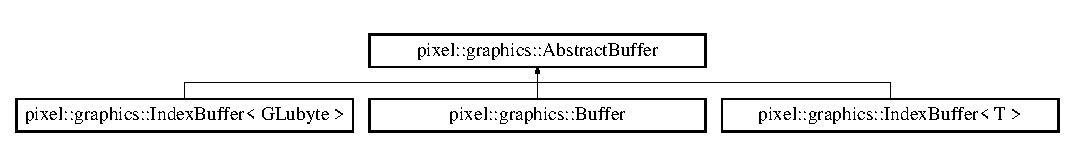
\includegraphics[height=1.536351cm]{classpixel_1_1graphics_1_1_abstract_buffer}
\end{center}
\end{figure}
\subsection*{Public Member Functions}
\begin{DoxyCompactItemize}
\item 
virtual void \hyperlink{classpixel_1_1graphics_1_1_abstract_buffer_a9d3bb463f35f08f5604012b7d22e113a}{bind} ()=0
\item 
virtual void \hyperlink{classpixel_1_1graphics_1_1_abstract_buffer_aee49569fa5c1767a40f2371ec96e40fc}{unbind} ()=0
\end{DoxyCompactItemize}


\subsection{Member Function Documentation}
\mbox{\Hypertarget{classpixel_1_1graphics_1_1_abstract_buffer_a9d3bb463f35f08f5604012b7d22e113a}\label{classpixel_1_1graphics_1_1_abstract_buffer_a9d3bb463f35f08f5604012b7d22e113a}} 
\index{pixel\+::graphics\+::\+Abstract\+Buffer@{pixel\+::graphics\+::\+Abstract\+Buffer}!bind@{bind}}
\index{bind@{bind}!pixel\+::graphics\+::\+Abstract\+Buffer@{pixel\+::graphics\+::\+Abstract\+Buffer}}
\subsubsection{\texorpdfstring{bind()}{bind()}}
{\footnotesize\ttfamily virtual void pixel\+::graphics\+::\+Abstract\+Buffer\+::bind (\begin{DoxyParamCaption}{ }\end{DoxyParamCaption})\hspace{0.3cm}{\ttfamily [pure virtual]}}



Implemented in \hyperlink{classpixel_1_1graphics_1_1_index_buffer_a70b8fdbdd19c8800e005425712426bde}{pixel\+::graphics\+::\+Index\+Buffer$<$ T $>$}, \hyperlink{classpixel_1_1graphics_1_1_index_buffer_a70b8fdbdd19c8800e005425712426bde}{pixel\+::graphics\+::\+Index\+Buffer$<$ G\+Lubyte $>$}, and \hyperlink{classpixel_1_1graphics_1_1_buffer_ab157f01d131d8416126607f71ab320ce}{pixel\+::graphics\+::\+Buffer}.

\mbox{\Hypertarget{classpixel_1_1graphics_1_1_abstract_buffer_aee49569fa5c1767a40f2371ec96e40fc}\label{classpixel_1_1graphics_1_1_abstract_buffer_aee49569fa5c1767a40f2371ec96e40fc}} 
\index{pixel\+::graphics\+::\+Abstract\+Buffer@{pixel\+::graphics\+::\+Abstract\+Buffer}!unbind@{unbind}}
\index{unbind@{unbind}!pixel\+::graphics\+::\+Abstract\+Buffer@{pixel\+::graphics\+::\+Abstract\+Buffer}}
\subsubsection{\texorpdfstring{unbind()}{unbind()}}
{\footnotesize\ttfamily virtual void pixel\+::graphics\+::\+Abstract\+Buffer\+::unbind (\begin{DoxyParamCaption}{ }\end{DoxyParamCaption})\hspace{0.3cm}{\ttfamily [pure virtual]}}



Implemented in \hyperlink{classpixel_1_1graphics_1_1_index_buffer_a5a90a44db73a048c76cf0fade5867621}{pixel\+::graphics\+::\+Index\+Buffer$<$ T $>$}, \hyperlink{classpixel_1_1graphics_1_1_index_buffer_a5a90a44db73a048c76cf0fade5867621}{pixel\+::graphics\+::\+Index\+Buffer$<$ G\+Lubyte $>$}, and \hyperlink{classpixel_1_1graphics_1_1_buffer_ac7b3cce29e02e3ee96322fee2ed8d624}{pixel\+::graphics\+::\+Buffer}.



The documentation for this class was generated from the following file\+:\begin{DoxyCompactItemize}
\item 
pixel/pixel/graphics/\hyperlink{buffer_8h}{buffer.\+h}\end{DoxyCompactItemize}

\hypertarget{structpixel_1_1_tileset_1_1_tile_1_1_animation}{}\section{pixel\+:\+:Tileset\+:\+:Tile\+:\+:Animation Struct Reference}
\label{structpixel_1_1_tileset_1_1_tile_1_1_animation}\index{pixel\+::\+Tileset\+::\+Tile\+::\+Animation@{pixel\+::\+Tileset\+::\+Tile\+::\+Animation}}


{\ttfamily \#include $<$pixel/tilemap/tileset.\+h$>$}

\subsection*{Classes}
\begin{DoxyCompactItemize}
\item 
struct \hyperlink{structpixel_1_1_tileset_1_1_tile_1_1_animation_1_1_frame}{Frame}
\end{DoxyCompactItemize}
\subsection*{Public Member Functions}
\begin{DoxyCompactItemize}
\item 
void \hyperlink{structpixel_1_1_tileset_1_1_tile_1_1_animation_a11f0be5eef21c355e1e423d1efe864c8}{add\+\_\+frame} (uint32\+\_\+t \hyperlink{structpixel_1_1_tileset_1_1_tile_aea8eb01c2f67c1cac8cbf12bbbf3d741}{tile\+\_\+id}, float duration)
\end{DoxyCompactItemize}
\subsection*{Public Attributes}
\begin{DoxyCompactItemize}
\item 
std\+::vector$<$ \hyperlink{structpixel_1_1_tileset_1_1_tile_1_1_animation_1_1_frame}{Frame} $>$ \hyperlink{structpixel_1_1_tileset_1_1_tile_1_1_animation_aa7752cf4088a9a395a0e5e470c906205}{frames} \{\}
\end{DoxyCompactItemize}


\subsection{Member Function Documentation}
\mbox{\Hypertarget{structpixel_1_1_tileset_1_1_tile_1_1_animation_a11f0be5eef21c355e1e423d1efe864c8}\label{structpixel_1_1_tileset_1_1_tile_1_1_animation_a11f0be5eef21c355e1e423d1efe864c8}} 
\index{pixel\+::\+Tileset\+::\+Tile\+::\+Animation@{pixel\+::\+Tileset\+::\+Tile\+::\+Animation}!add\+\_\+frame@{add\+\_\+frame}}
\index{add\+\_\+frame@{add\+\_\+frame}!pixel\+::\+Tileset\+::\+Tile\+::\+Animation@{pixel\+::\+Tileset\+::\+Tile\+::\+Animation}}
\subsubsection{\texorpdfstring{add\+\_\+frame()}{add\_frame()}}
{\footnotesize\ttfamily void pixel\+::\+Tileset\+::\+Tile\+::\+Animation\+::add\+\_\+frame (\begin{DoxyParamCaption}\item[{uint32\+\_\+t}]{tile\+\_\+id,  }\item[{float}]{duration }\end{DoxyParamCaption})\hspace{0.3cm}{\ttfamily [inline]}}



\subsection{Member Data Documentation}
\mbox{\Hypertarget{structpixel_1_1_tileset_1_1_tile_1_1_animation_aa7752cf4088a9a395a0e5e470c906205}\label{structpixel_1_1_tileset_1_1_tile_1_1_animation_aa7752cf4088a9a395a0e5e470c906205}} 
\index{pixel\+::\+Tileset\+::\+Tile\+::\+Animation@{pixel\+::\+Tileset\+::\+Tile\+::\+Animation}!frames@{frames}}
\index{frames@{frames}!pixel\+::\+Tileset\+::\+Tile\+::\+Animation@{pixel\+::\+Tileset\+::\+Tile\+::\+Animation}}
\subsubsection{\texorpdfstring{frames}{frames}}
{\footnotesize\ttfamily std\+::vector$<$\hyperlink{structpixel_1_1_tileset_1_1_tile_1_1_animation_1_1_frame}{Frame}$>$ pixel\+::\+Tileset\+::\+Tile\+::\+Animation\+::frames \{\}}



The documentation for this struct was generated from the following file\+:\begin{DoxyCompactItemize}
\item 
pixel/pixel/tilemap/\hyperlink{tileset_8h}{tileset.\+h}\end{DoxyCompactItemize}

\hypertarget{classpixel_1_1_app}{}\section{pixel\+:\+:App Class Reference}
\label{classpixel_1_1_app}\index{pixel\+::\+App@{pixel\+::\+App}}


{\ttfamily \#include $<$pixel/app/app.\+h$>$}

\subsection*{Public Member Functions}
\begin{DoxyCompactItemize}
\item 
\hyperlink{classpixel_1_1_app_af4a37ad9c00effc7cec0c255e03d70c4}{App} ()=default
\item 
\hyperlink{classpixel_1_1_app_a6fe4a8f0d585fb46ef777b772f33ee23}{App} (glm\+::ivec2 \hyperlink{app_8cpp_a93e893499cf4f577c814afbfefcef91e}{window\+\_\+size}, glm\+::vec4 \hyperlink{app_8cpp_a5fbf4b63994b492e6d4db94742408254}{clear\+\_\+color}, float pixel\+\_\+scale)
\item 
void \hyperlink{classpixel_1_1_app_a493e02e59da4f855f150da197c7635d2}{init} (int flags=0)
\item 
void \hyperlink{classpixel_1_1_app_ae09dc71078b64c56c673b1ad1d25b5d1}{run} ()
\item 
void \hyperlink{classpixel_1_1_app_a4c827ea9bb9a1d9c23a191e3cd5c9fd7}{set\+\_\+tick\+\_\+callback} (std\+::function$<$ void(void)$>$ cb)
\item 
void \hyperlink{classpixel_1_1_app_aeb5bd2f5b647c6d72e41675bbee75582}{late\+\_\+tick} ()
\item 
void \hyperlink{classpixel_1_1_app_a6bb62cf2cbcc3c7d161a0f94a75da1eb}{update\+\_\+render\+\_\+context} ()
\item 
G\+L\+F\+Wwindow $\ast$ \hyperlink{classpixel_1_1_app_a301a9d2271ae3bbd841d46412aec533d}{window} ()
\item 
\hyperlink{structpixel_1_1_render_context}{Render\+Context} \& \hyperlink{classpixel_1_1_app_a9200e57d78569df68303c9556f9bad8a}{render\+\_\+context} ()
\end{DoxyCompactItemize}
\subsection*{Private Member Functions}
\begin{DoxyCompactItemize}
\item 
void \hyperlink{classpixel_1_1_app_a100f1ea74491859e329bf4396c2ac4c7}{tick} ()
\end{DoxyCompactItemize}
\subsection*{Private Attributes}
\begin{DoxyCompactItemize}
\item 
int \hyperlink{classpixel_1_1_app_ad4382173f28f58facfa722cccbda6e4b}{frames\+\_\+} \{\}
\item 
G\+L\+F\+Wwindow $\ast$ \hyperlink{classpixel_1_1_app_aaec703aee9656cf040b8c9f5eb4fc3ad}{window\+\_\+}
\item 
std\+::function$<$ void(void)$>$ \hyperlink{classpixel_1_1_app_a5648c144f79952b5c4c51acf304fb2f8}{tick\+\_\+callback\+\_\+} \{\}
\item 
\hyperlink{classpixel_1_1time_1_1_frame_counter}{pixel\+::time\+::\+Frame\+Counter} \hyperlink{classpixel_1_1_app_ac247cd22d9e67b36b360d6ba827ad0e5}{fps\+\_\+counter\+\_\+} \{\}
\item 
\hyperlink{structpixel_1_1_render_context}{Render\+Context} \hyperlink{classpixel_1_1_app_ab118f43ae1840ff7fbdd771694dbe194}{render\+\_\+context\+\_\+}
\end{DoxyCompactItemize}


\subsection{Constructor \& Destructor Documentation}
\mbox{\Hypertarget{classpixel_1_1_app_af4a37ad9c00effc7cec0c255e03d70c4}\label{classpixel_1_1_app_af4a37ad9c00effc7cec0c255e03d70c4}} 
\index{pixel\+::\+App@{pixel\+::\+App}!App@{App}}
\index{App@{App}!pixel\+::\+App@{pixel\+::\+App}}
\subsubsection{\texorpdfstring{App()}{App()}\hspace{0.1cm}{\footnotesize\ttfamily [1/2]}}
{\footnotesize\ttfamily pixel\+::\+App\+::\+App (\begin{DoxyParamCaption}{ }\end{DoxyParamCaption})\hspace{0.3cm}{\ttfamily [default]}}

\mbox{\Hypertarget{classpixel_1_1_app_a6fe4a8f0d585fb46ef777b772f33ee23}\label{classpixel_1_1_app_a6fe4a8f0d585fb46ef777b772f33ee23}} 
\index{pixel\+::\+App@{pixel\+::\+App}!App@{App}}
\index{App@{App}!pixel\+::\+App@{pixel\+::\+App}}
\subsubsection{\texorpdfstring{App()}{App()}\hspace{0.1cm}{\footnotesize\ttfamily [2/2]}}
{\footnotesize\ttfamily App\+::\+App (\begin{DoxyParamCaption}\item[{glm\+::ivec2}]{window\+\_\+size,  }\item[{glm\+::vec4}]{clear\+\_\+color,  }\item[{float}]{pixel\+\_\+scale }\end{DoxyParamCaption})}



\subsection{Member Function Documentation}
\mbox{\Hypertarget{classpixel_1_1_app_a493e02e59da4f855f150da197c7635d2}\label{classpixel_1_1_app_a493e02e59da4f855f150da197c7635d2}} 
\index{pixel\+::\+App@{pixel\+::\+App}!init@{init}}
\index{init@{init}!pixel\+::\+App@{pixel\+::\+App}}
\subsubsection{\texorpdfstring{init()}{init()}}
{\footnotesize\ttfamily void App\+::init (\begin{DoxyParamCaption}\item[{int}]{flags = {\ttfamily 0} }\end{DoxyParamCaption})}

\mbox{\Hypertarget{classpixel_1_1_app_aeb5bd2f5b647c6d72e41675bbee75582}\label{classpixel_1_1_app_aeb5bd2f5b647c6d72e41675bbee75582}} 
\index{pixel\+::\+App@{pixel\+::\+App}!late\+\_\+tick@{late\+\_\+tick}}
\index{late\+\_\+tick@{late\+\_\+tick}!pixel\+::\+App@{pixel\+::\+App}}
\subsubsection{\texorpdfstring{late\+\_\+tick()}{late\_tick()}}
{\footnotesize\ttfamily void App\+::late\+\_\+tick (\begin{DoxyParamCaption}{ }\end{DoxyParamCaption})}

\mbox{\Hypertarget{classpixel_1_1_app_a9200e57d78569df68303c9556f9bad8a}\label{classpixel_1_1_app_a9200e57d78569df68303c9556f9bad8a}} 
\index{pixel\+::\+App@{pixel\+::\+App}!render\+\_\+context@{render\+\_\+context}}
\index{render\+\_\+context@{render\+\_\+context}!pixel\+::\+App@{pixel\+::\+App}}
\subsubsection{\texorpdfstring{render\+\_\+context()}{render\_context()}}
{\footnotesize\ttfamily \hyperlink{structpixel_1_1_render_context}{Render\+Context} \& App\+::render\+\_\+context (\begin{DoxyParamCaption}{ }\end{DoxyParamCaption})}

\mbox{\Hypertarget{classpixel_1_1_app_ae09dc71078b64c56c673b1ad1d25b5d1}\label{classpixel_1_1_app_ae09dc71078b64c56c673b1ad1d25b5d1}} 
\index{pixel\+::\+App@{pixel\+::\+App}!run@{run}}
\index{run@{run}!pixel\+::\+App@{pixel\+::\+App}}
\subsubsection{\texorpdfstring{run()}{run()}}
{\footnotesize\ttfamily void App\+::run (\begin{DoxyParamCaption}{ }\end{DoxyParamCaption})}

\mbox{\Hypertarget{classpixel_1_1_app_a4c827ea9bb9a1d9c23a191e3cd5c9fd7}\label{classpixel_1_1_app_a4c827ea9bb9a1d9c23a191e3cd5c9fd7}} 
\index{pixel\+::\+App@{pixel\+::\+App}!set\+\_\+tick\+\_\+callback@{set\+\_\+tick\+\_\+callback}}
\index{set\+\_\+tick\+\_\+callback@{set\+\_\+tick\+\_\+callback}!pixel\+::\+App@{pixel\+::\+App}}
\subsubsection{\texorpdfstring{set\+\_\+tick\+\_\+callback()}{set\_tick\_callback()}}
{\footnotesize\ttfamily void App\+::set\+\_\+tick\+\_\+callback (\begin{DoxyParamCaption}\item[{std\+::function$<$ void(void)$>$}]{cb }\end{DoxyParamCaption})}

\mbox{\Hypertarget{classpixel_1_1_app_a100f1ea74491859e329bf4396c2ac4c7}\label{classpixel_1_1_app_a100f1ea74491859e329bf4396c2ac4c7}} 
\index{pixel\+::\+App@{pixel\+::\+App}!tick@{tick}}
\index{tick@{tick}!pixel\+::\+App@{pixel\+::\+App}}
\subsubsection{\texorpdfstring{tick()}{tick()}}
{\footnotesize\ttfamily void App\+::tick (\begin{DoxyParamCaption}{ }\end{DoxyParamCaption})\hspace{0.3cm}{\ttfamily [private]}}

\mbox{\Hypertarget{classpixel_1_1_app_a6bb62cf2cbcc3c7d161a0f94a75da1eb}\label{classpixel_1_1_app_a6bb62cf2cbcc3c7d161a0f94a75da1eb}} 
\index{pixel\+::\+App@{pixel\+::\+App}!update\+\_\+render\+\_\+context@{update\+\_\+render\+\_\+context}}
\index{update\+\_\+render\+\_\+context@{update\+\_\+render\+\_\+context}!pixel\+::\+App@{pixel\+::\+App}}
\subsubsection{\texorpdfstring{update\+\_\+render\+\_\+context()}{update\_render\_context()}}
{\footnotesize\ttfamily void App\+::update\+\_\+render\+\_\+context (\begin{DoxyParamCaption}{ }\end{DoxyParamCaption})}

\mbox{\Hypertarget{classpixel_1_1_app_a301a9d2271ae3bbd841d46412aec533d}\label{classpixel_1_1_app_a301a9d2271ae3bbd841d46412aec533d}} 
\index{pixel\+::\+App@{pixel\+::\+App}!window@{window}}
\index{window@{window}!pixel\+::\+App@{pixel\+::\+App}}
\subsubsection{\texorpdfstring{window()}{window()}}
{\footnotesize\ttfamily G\+L\+F\+Wwindow $\ast$ App\+::window (\begin{DoxyParamCaption}{ }\end{DoxyParamCaption})}



\subsection{Member Data Documentation}
\mbox{\Hypertarget{classpixel_1_1_app_ac247cd22d9e67b36b360d6ba827ad0e5}\label{classpixel_1_1_app_ac247cd22d9e67b36b360d6ba827ad0e5}} 
\index{pixel\+::\+App@{pixel\+::\+App}!fps\+\_\+counter\+\_\+@{fps\+\_\+counter\+\_\+}}
\index{fps\+\_\+counter\+\_\+@{fps\+\_\+counter\+\_\+}!pixel\+::\+App@{pixel\+::\+App}}
\subsubsection{\texorpdfstring{fps\+\_\+counter\+\_\+}{fps\_counter\_}}
{\footnotesize\ttfamily \hyperlink{classpixel_1_1time_1_1_frame_counter}{pixel\+::time\+::\+Frame\+Counter} pixel\+::\+App\+::fps\+\_\+counter\+\_\+ \{\}\hspace{0.3cm}{\ttfamily [private]}}

\mbox{\Hypertarget{classpixel_1_1_app_ad4382173f28f58facfa722cccbda6e4b}\label{classpixel_1_1_app_ad4382173f28f58facfa722cccbda6e4b}} 
\index{pixel\+::\+App@{pixel\+::\+App}!frames\+\_\+@{frames\+\_\+}}
\index{frames\+\_\+@{frames\+\_\+}!pixel\+::\+App@{pixel\+::\+App}}
\subsubsection{\texorpdfstring{frames\+\_\+}{frames\_}}
{\footnotesize\ttfamily int pixel\+::\+App\+::frames\+\_\+ \{\}\hspace{0.3cm}{\ttfamily [private]}}

\mbox{\Hypertarget{classpixel_1_1_app_ab118f43ae1840ff7fbdd771694dbe194}\label{classpixel_1_1_app_ab118f43ae1840ff7fbdd771694dbe194}} 
\index{pixel\+::\+App@{pixel\+::\+App}!render\+\_\+context\+\_\+@{render\+\_\+context\+\_\+}}
\index{render\+\_\+context\+\_\+@{render\+\_\+context\+\_\+}!pixel\+::\+App@{pixel\+::\+App}}
\subsubsection{\texorpdfstring{render\+\_\+context\+\_\+}{render\_context\_}}
{\footnotesize\ttfamily \hyperlink{structpixel_1_1_render_context}{Render\+Context} pixel\+::\+App\+::render\+\_\+context\+\_\+\hspace{0.3cm}{\ttfamily [private]}}

{\bfseries Initial value\+:}
\begin{DoxyCode}
\{
        \hyperlink{namespacepixel_a9c38287d50c84fb5c1f25c965db0a6a5}{DEFAULT\_WINDOW\_SIZE},
        \hyperlink{namespacepixel_aa4c296a437eb1e0def40cff29b699be2}{DEFAULT\_CLEAR\_COLOR},
        \hyperlink{namespacepixel_ae08ee7e855f850855389107cb37ae167}{DEFAULT\_PIXEL\_SCALE}
    \}
\end{DoxyCode}
\mbox{\Hypertarget{classpixel_1_1_app_a5648c144f79952b5c4c51acf304fb2f8}\label{classpixel_1_1_app_a5648c144f79952b5c4c51acf304fb2f8}} 
\index{pixel\+::\+App@{pixel\+::\+App}!tick\+\_\+callback\+\_\+@{tick\+\_\+callback\+\_\+}}
\index{tick\+\_\+callback\+\_\+@{tick\+\_\+callback\+\_\+}!pixel\+::\+App@{pixel\+::\+App}}
\subsubsection{\texorpdfstring{tick\+\_\+callback\+\_\+}{tick\_callback\_}}
{\footnotesize\ttfamily std\+::function$<$void(void)$>$ pixel\+::\+App\+::tick\+\_\+callback\+\_\+ \{\}\hspace{0.3cm}{\ttfamily [private]}}

\mbox{\Hypertarget{classpixel_1_1_app_aaec703aee9656cf040b8c9f5eb4fc3ad}\label{classpixel_1_1_app_aaec703aee9656cf040b8c9f5eb4fc3ad}} 
\index{pixel\+::\+App@{pixel\+::\+App}!window\+\_\+@{window\+\_\+}}
\index{window\+\_\+@{window\+\_\+}!pixel\+::\+App@{pixel\+::\+App}}
\subsubsection{\texorpdfstring{window\+\_\+}{window\_}}
{\footnotesize\ttfamily G\+L\+F\+Wwindow$\ast$ pixel\+::\+App\+::window\+\_\+\hspace{0.3cm}{\ttfamily [private]}}



The documentation for this class was generated from the following files\+:\begin{DoxyCompactItemize}
\item 
pixel/pixel/app/\hyperlink{app_8h}{app.\+h}\item 
pixel/pixel/app/\hyperlink{app_8cpp}{app.\+cpp}\end{DoxyCompactItemize}

\hypertarget{classpixel_1_1_argument_error}{}\section{pixel\+:\+:Argument\+Error Class Reference}
\label{classpixel_1_1_argument_error}\index{pixel\+::\+Argument\+Error@{pixel\+::\+Argument\+Error}}


Exception thrown when argument to method or function is not acceptable.  




{\ttfamily \#include $<$pixel/error.\+h$>$}

Inheritance diagram for pixel\+:\+:Argument\+Error\+:\begin{figure}[H]
\begin{center}
\leavevmode
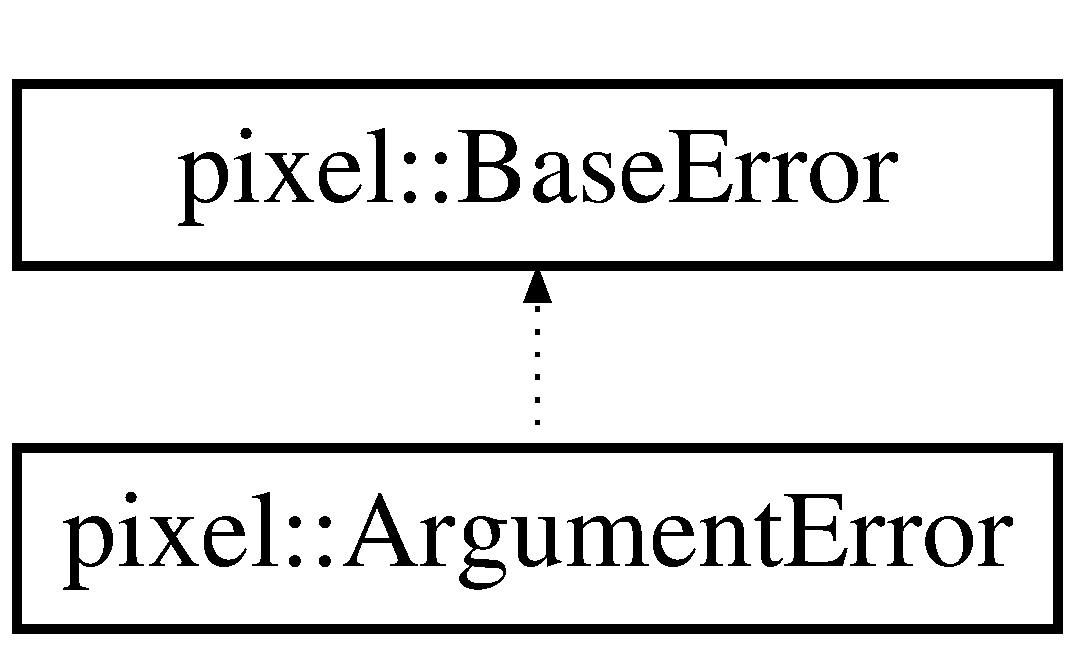
\includegraphics[height=2.000000cm]{classpixel_1_1_argument_error}
\end{center}
\end{figure}
\subsection*{Additional Inherited Members}


\subsection{Detailed Description}
Exception thrown when argument to method or function is not acceptable. 

The documentation for this class was generated from the following file\+:\begin{DoxyCompactItemize}
\item 
pixel/pixel/\hyperlink{error_8h}{error.\+h}\end{DoxyCompactItemize}

\hypertarget{structpixel_1_1graphics_1_1_attribute}{}\section{pixel\+:\+:graphics\+:\+:Attribute Struct Reference}
\label{structpixel_1_1graphics_1_1_attribute}\index{pixel\+::graphics\+::\+Attribute@{pixel\+::graphics\+::\+Attribute}}


{\ttfamily \#include $<$pixel/graphics/attribute.\+h$>$}

\subsection*{Public Member Functions}
\begin{DoxyCompactItemize}
\item 
std\+::string \hyperlink{structpixel_1_1graphics_1_1_attribute_abbf0a8cc12603b77f26dee1b841cdac8}{debug\+Print} () const
\end{DoxyCompactItemize}
\subsection*{Public Attributes}
\begin{DoxyCompactItemize}
\item 
unsigned int \hyperlink{structpixel_1_1graphics_1_1_attribute_ae0945b760635b2a95aa5620a638ebae8}{index}
\item 
int \hyperlink{structpixel_1_1graphics_1_1_attribute_a7657461b957ab3c74d3a6dc237f1581d}{size}
\item 
int \hyperlink{structpixel_1_1graphics_1_1_attribute_a4547040e98863207d138e265941781ef}{location}
\item 
unsigned int \hyperlink{structpixel_1_1graphics_1_1_attribute_a47a5857b9ac8a25c031e14e083afaf59}{type}
\item 
std\+::string \hyperlink{structpixel_1_1graphics_1_1_attribute_a8ebe8a0e5d3868da41d7c0c54163507c}{name}
\end{DoxyCompactItemize}


\subsection{Member Function Documentation}
\mbox{\Hypertarget{structpixel_1_1graphics_1_1_attribute_abbf0a8cc12603b77f26dee1b841cdac8}\label{structpixel_1_1graphics_1_1_attribute_abbf0a8cc12603b77f26dee1b841cdac8}} 
\index{pixel\+::graphics\+::\+Attribute@{pixel\+::graphics\+::\+Attribute}!debug\+Print@{debug\+Print}}
\index{debug\+Print@{debug\+Print}!pixel\+::graphics\+::\+Attribute@{pixel\+::graphics\+::\+Attribute}}
\subsubsection{\texorpdfstring{debug\+Print()}{debugPrint()}}
{\footnotesize\ttfamily std\+::string Attribute\+::debug\+Print (\begin{DoxyParamCaption}{ }\end{DoxyParamCaption}) const}



\subsection{Member Data Documentation}
\mbox{\Hypertarget{structpixel_1_1graphics_1_1_attribute_ae0945b760635b2a95aa5620a638ebae8}\label{structpixel_1_1graphics_1_1_attribute_ae0945b760635b2a95aa5620a638ebae8}} 
\index{pixel\+::graphics\+::\+Attribute@{pixel\+::graphics\+::\+Attribute}!index@{index}}
\index{index@{index}!pixel\+::graphics\+::\+Attribute@{pixel\+::graphics\+::\+Attribute}}
\subsubsection{\texorpdfstring{index}{index}}
{\footnotesize\ttfamily unsigned int pixel\+::graphics\+::\+Attribute\+::index}

\mbox{\Hypertarget{structpixel_1_1graphics_1_1_attribute_a4547040e98863207d138e265941781ef}\label{structpixel_1_1graphics_1_1_attribute_a4547040e98863207d138e265941781ef}} 
\index{pixel\+::graphics\+::\+Attribute@{pixel\+::graphics\+::\+Attribute}!location@{location}}
\index{location@{location}!pixel\+::graphics\+::\+Attribute@{pixel\+::graphics\+::\+Attribute}}
\subsubsection{\texorpdfstring{location}{location}}
{\footnotesize\ttfamily int pixel\+::graphics\+::\+Attribute\+::location}

\mbox{\Hypertarget{structpixel_1_1graphics_1_1_attribute_a8ebe8a0e5d3868da41d7c0c54163507c}\label{structpixel_1_1graphics_1_1_attribute_a8ebe8a0e5d3868da41d7c0c54163507c}} 
\index{pixel\+::graphics\+::\+Attribute@{pixel\+::graphics\+::\+Attribute}!name@{name}}
\index{name@{name}!pixel\+::graphics\+::\+Attribute@{pixel\+::graphics\+::\+Attribute}}
\subsubsection{\texorpdfstring{name}{name}}
{\footnotesize\ttfamily std\+::string pixel\+::graphics\+::\+Attribute\+::name}

\mbox{\Hypertarget{structpixel_1_1graphics_1_1_attribute_a7657461b957ab3c74d3a6dc237f1581d}\label{structpixel_1_1graphics_1_1_attribute_a7657461b957ab3c74d3a6dc237f1581d}} 
\index{pixel\+::graphics\+::\+Attribute@{pixel\+::graphics\+::\+Attribute}!size@{size}}
\index{size@{size}!pixel\+::graphics\+::\+Attribute@{pixel\+::graphics\+::\+Attribute}}
\subsubsection{\texorpdfstring{size}{size}}
{\footnotesize\ttfamily int pixel\+::graphics\+::\+Attribute\+::size}

\mbox{\Hypertarget{structpixel_1_1graphics_1_1_attribute_a47a5857b9ac8a25c031e14e083afaf59}\label{structpixel_1_1graphics_1_1_attribute_a47a5857b9ac8a25c031e14e083afaf59}} 
\index{pixel\+::graphics\+::\+Attribute@{pixel\+::graphics\+::\+Attribute}!type@{type}}
\index{type@{type}!pixel\+::graphics\+::\+Attribute@{pixel\+::graphics\+::\+Attribute}}
\subsubsection{\texorpdfstring{type}{type}}
{\footnotesize\ttfamily unsigned int pixel\+::graphics\+::\+Attribute\+::type}



The documentation for this struct was generated from the following files\+:\begin{DoxyCompactItemize}
\item 
pixel/pixel/graphics/\hyperlink{attribute_8h}{attribute.\+h}\item 
pixel/pixel/graphics/\hyperlink{attribute_8cpp}{attribute.\+cpp}\end{DoxyCompactItemize}

\hypertarget{classpixel_1_1_base_error}{}\section{pixel\+:\+:Base\+Error Class Reference}
\label{classpixel_1_1_base_error}\index{pixel\+::\+Base\+Error@{pixel\+::\+Base\+Error}}


Base exception class.  




{\ttfamily \#include $<$pixel/error.\+h$>$}

Inheritance diagram for pixel\+:\+:Base\+Error\+:\begin{figure}[H]
\begin{center}
\leavevmode
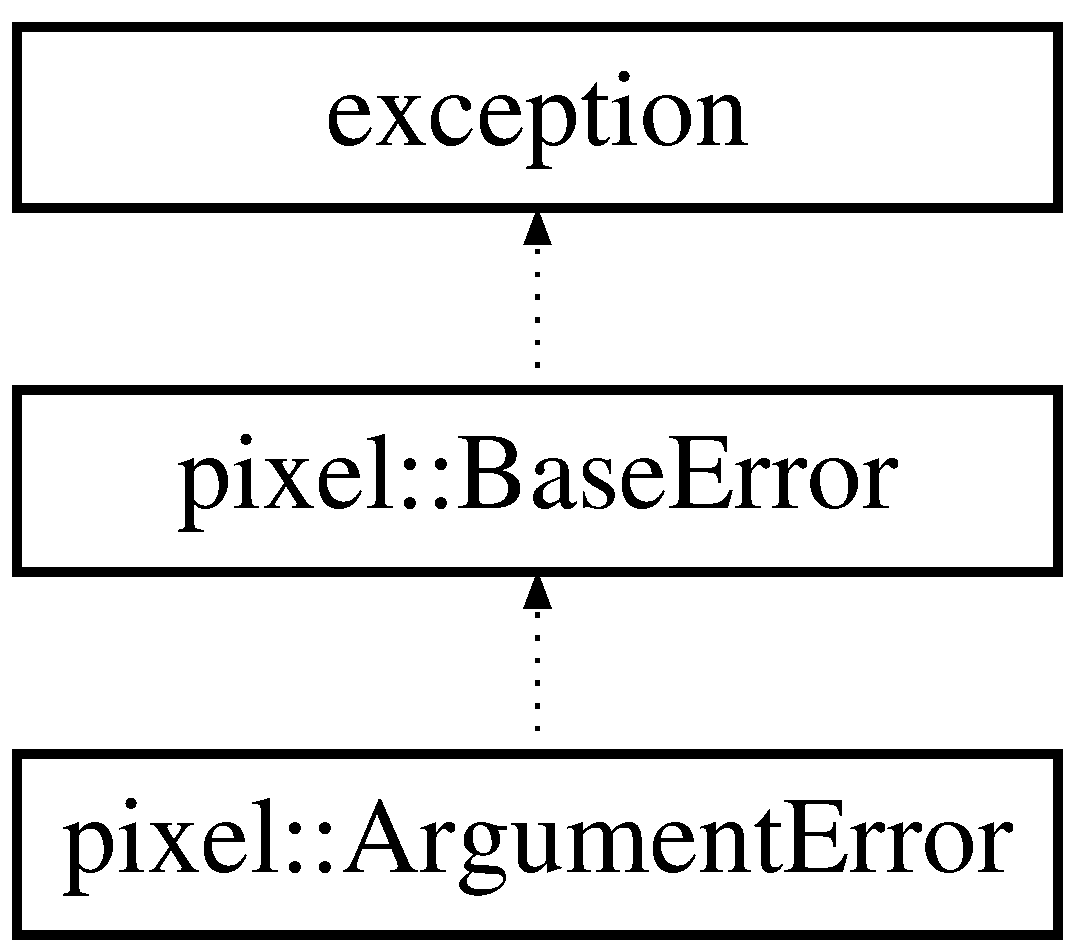
\includegraphics[height=3.000000cm]{classpixel_1_1_base_error}
\end{center}
\end{figure}
\subsection*{Public Member Functions}
\begin{DoxyCompactItemize}
\item 
\hyperlink{classpixel_1_1_base_error_aee0432935f72987286c9d4518642269e}{Base\+Error} (std\+::string m)
\item 
virtual const char $\ast$ \hyperlink{classpixel_1_1_base_error_a7e3a7f00803f17d146be69cb0f8e3f95}{what} () const noexcept override
\end{DoxyCompactItemize}
\subsection*{Private Attributes}
\begin{DoxyCompactItemize}
\item 
std\+::string \hyperlink{classpixel_1_1_base_error_a237babe03722b7f9c1ae03819bf88754}{msg\+\_\+}
\end{DoxyCompactItemize}


\subsection{Detailed Description}
Base exception class. 

Requires error string for construction. 

\subsection{Constructor \& Destructor Documentation}
\mbox{\Hypertarget{classpixel_1_1_base_error_aee0432935f72987286c9d4518642269e}\label{classpixel_1_1_base_error_aee0432935f72987286c9d4518642269e}} 
\index{pixel\+::\+Base\+Error@{pixel\+::\+Base\+Error}!Base\+Error@{Base\+Error}}
\index{Base\+Error@{Base\+Error}!pixel\+::\+Base\+Error@{pixel\+::\+Base\+Error}}
\subsubsection{\texorpdfstring{Base\+Error()}{BaseError()}}
{\footnotesize\ttfamily pixel\+::\+Base\+Error\+::\+Base\+Error (\begin{DoxyParamCaption}\item[{std\+::string}]{m }\end{DoxyParamCaption})\hspace{0.3cm}{\ttfamily [inline]}}



\subsection{Member Function Documentation}
\mbox{\Hypertarget{classpixel_1_1_base_error_a7e3a7f00803f17d146be69cb0f8e3f95}\label{classpixel_1_1_base_error_a7e3a7f00803f17d146be69cb0f8e3f95}} 
\index{pixel\+::\+Base\+Error@{pixel\+::\+Base\+Error}!what@{what}}
\index{what@{what}!pixel\+::\+Base\+Error@{pixel\+::\+Base\+Error}}
\subsubsection{\texorpdfstring{what()}{what()}}
{\footnotesize\ttfamily virtual const char$\ast$ pixel\+::\+Base\+Error\+::what (\begin{DoxyParamCaption}{ }\end{DoxyParamCaption}) const\hspace{0.3cm}{\ttfamily [inline]}, {\ttfamily [override]}, {\ttfamily [virtual]}, {\ttfamily [noexcept]}}



\subsection{Member Data Documentation}
\mbox{\Hypertarget{classpixel_1_1_base_error_a237babe03722b7f9c1ae03819bf88754}\label{classpixel_1_1_base_error_a237babe03722b7f9c1ae03819bf88754}} 
\index{pixel\+::\+Base\+Error@{pixel\+::\+Base\+Error}!msg\+\_\+@{msg\+\_\+}}
\index{msg\+\_\+@{msg\+\_\+}!pixel\+::\+Base\+Error@{pixel\+::\+Base\+Error}}
\subsubsection{\texorpdfstring{msg\+\_\+}{msg\_}}
{\footnotesize\ttfamily std\+::string pixel\+::\+Base\+Error\+::msg\+\_\+\hspace{0.3cm}{\ttfamily [private]}}



The documentation for this class was generated from the following file\+:\begin{DoxyCompactItemize}
\item 
pixel/pixel/\hyperlink{error_8h}{error.\+h}\end{DoxyCompactItemize}

\hypertarget{classpixel_1_1graphics_1_1_buffer}{}\section{pixel\+:\+:graphics\+:\+:Buffer Class Reference}
\label{classpixel_1_1graphics_1_1_buffer}\index{pixel\+::graphics\+::\+Buffer@{pixel\+::graphics\+::\+Buffer}}


{\ttfamily \#include $<$pixel/graphics/buffer.\+h$>$}

Inheritance diagram for pixel\+:\+:graphics\+:\+:Buffer\+:\begin{figure}[H]
\begin{center}
\leavevmode
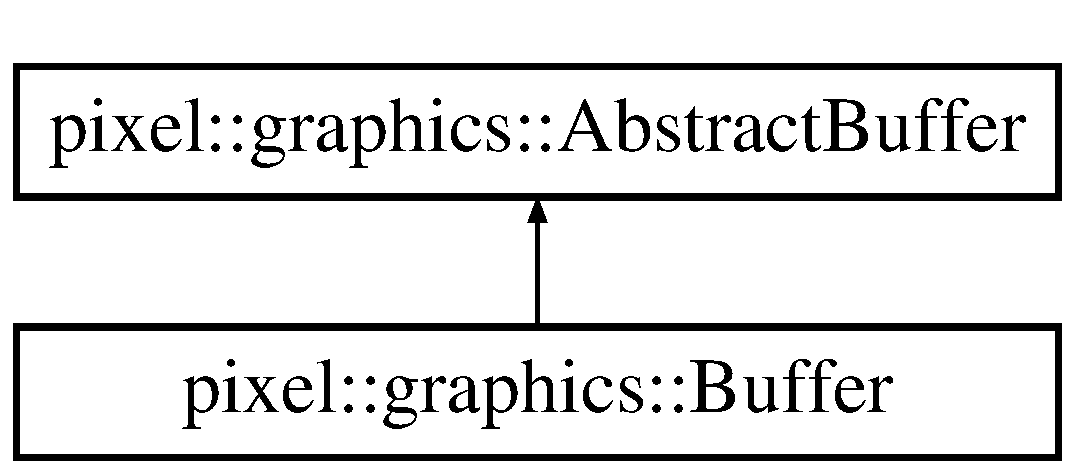
\includegraphics[height=2.000000cm]{classpixel_1_1graphics_1_1_buffer}
\end{center}
\end{figure}
\subsection*{Public Member Functions}
\begin{DoxyCompactItemize}
\item 
\hyperlink{classpixel_1_1graphics_1_1_buffer_a9fa35b1875e9c79e088587d23d6009c5}{Buffer} ()
\item 
\hyperlink{classpixel_1_1graphics_1_1_buffer_aa1c31a950ba27ec02845463158760fc1}{Buffer} (G\+Lenum usage\+Hint)
\item 
void \hyperlink{classpixel_1_1graphics_1_1_buffer_ae6521f1a22946dc2e23775cef722adca}{bind\+To\+Program\+Attribute} (const \hyperlink{classpixel_1_1graphics_1_1_shader}{Shader} \&program, const std\+::string \&name, int stride=0, int offset=0, int divisor=0)
\item 
void \hyperlink{classpixel_1_1graphics_1_1_buffer_a4454068cd191da9ff2133d22f53611fd}{load\+Data} (const void $\ast$data, const size\+\_\+t \hyperlink{namespacepixel_a465745e3b1a334686475c629948876f0}{size})
\item 
void \hyperlink{classpixel_1_1graphics_1_1_buffer_ab157f01d131d8416126607f71ab320ce}{bind} () override
\item 
void \hyperlink{classpixel_1_1graphics_1_1_buffer_ac7b3cce29e02e3ee96322fee2ed8d624}{unbind} () override
\end{DoxyCompactItemize}
\subsection*{Public Attributes}
\begin{DoxyCompactItemize}
\item 
G\+Luint \hyperlink{classpixel_1_1graphics_1_1_buffer_a3c9df71bba83b43e11784699cdc0d44a}{buffer\+\_\+id\+\_\+} \{\}
\item 
G\+Lenum \hyperlink{classpixel_1_1graphics_1_1_buffer_a8c1f22b44385b66d4b05a6f4d7f6a6ba}{usage\+\_\+hint\+\_\+} \{\}
\end{DoxyCompactItemize}


\subsection{Constructor \& Destructor Documentation}
\mbox{\Hypertarget{classpixel_1_1graphics_1_1_buffer_a9fa35b1875e9c79e088587d23d6009c5}\label{classpixel_1_1graphics_1_1_buffer_a9fa35b1875e9c79e088587d23d6009c5}} 
\index{pixel\+::graphics\+::\+Buffer@{pixel\+::graphics\+::\+Buffer}!Buffer@{Buffer}}
\index{Buffer@{Buffer}!pixel\+::graphics\+::\+Buffer@{pixel\+::graphics\+::\+Buffer}}
\subsubsection{\texorpdfstring{Buffer()}{Buffer()}\hspace{0.1cm}{\footnotesize\ttfamily [1/2]}}
{\footnotesize\ttfamily pixel\+::graphics\+::\+Buffer\+::\+Buffer (\begin{DoxyParamCaption}{ }\end{DoxyParamCaption})}

\mbox{\Hypertarget{classpixel_1_1graphics_1_1_buffer_aa1c31a950ba27ec02845463158760fc1}\label{classpixel_1_1graphics_1_1_buffer_aa1c31a950ba27ec02845463158760fc1}} 
\index{pixel\+::graphics\+::\+Buffer@{pixel\+::graphics\+::\+Buffer}!Buffer@{Buffer}}
\index{Buffer@{Buffer}!pixel\+::graphics\+::\+Buffer@{pixel\+::graphics\+::\+Buffer}}
\subsubsection{\texorpdfstring{Buffer()}{Buffer()}\hspace{0.1cm}{\footnotesize\ttfamily [2/2]}}
{\footnotesize\ttfamily pixel\+::graphics\+::\+Buffer\+::\+Buffer (\begin{DoxyParamCaption}\item[{G\+Lenum}]{usage\+Hint }\end{DoxyParamCaption})\hspace{0.3cm}{\ttfamily [explicit]}}



\subsection{Member Function Documentation}
\mbox{\Hypertarget{classpixel_1_1graphics_1_1_buffer_ab157f01d131d8416126607f71ab320ce}\label{classpixel_1_1graphics_1_1_buffer_ab157f01d131d8416126607f71ab320ce}} 
\index{pixel\+::graphics\+::\+Buffer@{pixel\+::graphics\+::\+Buffer}!bind@{bind}}
\index{bind@{bind}!pixel\+::graphics\+::\+Buffer@{pixel\+::graphics\+::\+Buffer}}
\subsubsection{\texorpdfstring{bind()}{bind()}}
{\footnotesize\ttfamily void pixel\+::graphics\+::\+Buffer\+::bind (\begin{DoxyParamCaption}{ }\end{DoxyParamCaption})\hspace{0.3cm}{\ttfamily [override]}, {\ttfamily [virtual]}}



Implements \hyperlink{classpixel_1_1graphics_1_1_abstract_buffer_a9d3bb463f35f08f5604012b7d22e113a}{pixel\+::graphics\+::\+Abstract\+Buffer}.

\mbox{\Hypertarget{classpixel_1_1graphics_1_1_buffer_ae6521f1a22946dc2e23775cef722adca}\label{classpixel_1_1graphics_1_1_buffer_ae6521f1a22946dc2e23775cef722adca}} 
\index{pixel\+::graphics\+::\+Buffer@{pixel\+::graphics\+::\+Buffer}!bind\+To\+Program\+Attribute@{bind\+To\+Program\+Attribute}}
\index{bind\+To\+Program\+Attribute@{bind\+To\+Program\+Attribute}!pixel\+::graphics\+::\+Buffer@{pixel\+::graphics\+::\+Buffer}}
\subsubsection{\texorpdfstring{bind\+To\+Program\+Attribute()}{bindToProgramAttribute()}}
{\footnotesize\ttfamily void pixel\+::graphics\+::\+Buffer\+::bind\+To\+Program\+Attribute (\begin{DoxyParamCaption}\item[{const \hyperlink{classpixel_1_1graphics_1_1_shader}{Shader} \&}]{program,  }\item[{const std\+::string \&}]{name,  }\item[{int}]{stride = {\ttfamily 0},  }\item[{int}]{offset = {\ttfamily 0},  }\item[{int}]{divisor = {\ttfamily 0} }\end{DoxyParamCaption})}

\mbox{\Hypertarget{classpixel_1_1graphics_1_1_buffer_a4454068cd191da9ff2133d22f53611fd}\label{classpixel_1_1graphics_1_1_buffer_a4454068cd191da9ff2133d22f53611fd}} 
\index{pixel\+::graphics\+::\+Buffer@{pixel\+::graphics\+::\+Buffer}!load\+Data@{load\+Data}}
\index{load\+Data@{load\+Data}!pixel\+::graphics\+::\+Buffer@{pixel\+::graphics\+::\+Buffer}}
\subsubsection{\texorpdfstring{load\+Data()}{loadData()}}
{\footnotesize\ttfamily void pixel\+::graphics\+::\+Buffer\+::load\+Data (\begin{DoxyParamCaption}\item[{const void $\ast$}]{data,  }\item[{const size\+\_\+t}]{size }\end{DoxyParamCaption})}

\mbox{\Hypertarget{classpixel_1_1graphics_1_1_buffer_ac7b3cce29e02e3ee96322fee2ed8d624}\label{classpixel_1_1graphics_1_1_buffer_ac7b3cce29e02e3ee96322fee2ed8d624}} 
\index{pixel\+::graphics\+::\+Buffer@{pixel\+::graphics\+::\+Buffer}!unbind@{unbind}}
\index{unbind@{unbind}!pixel\+::graphics\+::\+Buffer@{pixel\+::graphics\+::\+Buffer}}
\subsubsection{\texorpdfstring{unbind()}{unbind()}}
{\footnotesize\ttfamily void pixel\+::graphics\+::\+Buffer\+::unbind (\begin{DoxyParamCaption}{ }\end{DoxyParamCaption})\hspace{0.3cm}{\ttfamily [override]}, {\ttfamily [virtual]}}



Implements \hyperlink{classpixel_1_1graphics_1_1_abstract_buffer_aee49569fa5c1767a40f2371ec96e40fc}{pixel\+::graphics\+::\+Abstract\+Buffer}.



\subsection{Member Data Documentation}
\mbox{\Hypertarget{classpixel_1_1graphics_1_1_buffer_a3c9df71bba83b43e11784699cdc0d44a}\label{classpixel_1_1graphics_1_1_buffer_a3c9df71bba83b43e11784699cdc0d44a}} 
\index{pixel\+::graphics\+::\+Buffer@{pixel\+::graphics\+::\+Buffer}!buffer\+\_\+id\+\_\+@{buffer\+\_\+id\+\_\+}}
\index{buffer\+\_\+id\+\_\+@{buffer\+\_\+id\+\_\+}!pixel\+::graphics\+::\+Buffer@{pixel\+::graphics\+::\+Buffer}}
\subsubsection{\texorpdfstring{buffer\+\_\+id\+\_\+}{buffer\_id\_}}
{\footnotesize\ttfamily G\+Luint pixel\+::graphics\+::\+Buffer\+::buffer\+\_\+id\+\_\+ \{\}}

\mbox{\Hypertarget{classpixel_1_1graphics_1_1_buffer_a8c1f22b44385b66d4b05a6f4d7f6a6ba}\label{classpixel_1_1graphics_1_1_buffer_a8c1f22b44385b66d4b05a6f4d7f6a6ba}} 
\index{pixel\+::graphics\+::\+Buffer@{pixel\+::graphics\+::\+Buffer}!usage\+\_\+hint\+\_\+@{usage\+\_\+hint\+\_\+}}
\index{usage\+\_\+hint\+\_\+@{usage\+\_\+hint\+\_\+}!pixel\+::graphics\+::\+Buffer@{pixel\+::graphics\+::\+Buffer}}
\subsubsection{\texorpdfstring{usage\+\_\+hint\+\_\+}{usage\_hint\_}}
{\footnotesize\ttfamily G\+Lenum pixel\+::graphics\+::\+Buffer\+::usage\+\_\+hint\+\_\+ \{\}}



The documentation for this class was generated from the following files\+:\begin{DoxyCompactItemize}
\item 
pixel/pixel/graphics/\hyperlink{buffer_8h}{buffer.\+h}\item 
pixel/pixel/graphics/\hyperlink{buffer_8cpp}{buffer.\+cpp}\end{DoxyCompactItemize}

\hypertarget{classpixel_1_1graphics_1_1_camera}{}\section{pixel\+:\+:graphics\+:\+:Camera Class Reference}
\label{classpixel_1_1graphics_1_1_camera}\index{pixel\+::graphics\+::\+Camera@{pixel\+::graphics\+::\+Camera}}


{\ttfamily \#include $<$pixel/graphics/camera.\+h$>$}

\subsection*{Public Member Functions}
\begin{DoxyCompactItemize}
\item 
\hyperlink{classpixel_1_1graphics_1_1_camera_ab919425fc4978e0846a19a9ff446b621}{Camera} (const glm\+::ivec2 \&\hyperlink{classpixel_1_1graphics_1_1_camera_aa8bad1ecf68611262195b74f42151922}{window\+\_\+size}, const glm\+::vec4 \&bounds)
\item 
\hyperlink{classpixel_1_1graphics_1_1_camera_a0c6568dcfd5bf88473afdce0e37a8626}{Camera} ()=default
\item 
void \hyperlink{classpixel_1_1graphics_1_1_camera_a9dce6fdffb32d923fbcf0e843d907646}{lock\+\_\+x} (bool lock=true)
\item 
void \hyperlink{classpixel_1_1graphics_1_1_camera_a625c61d63849d8c3776002629c5b790c}{lock\+\_\+y} (bool lock=true)
\item 
void \hyperlink{classpixel_1_1graphics_1_1_camera_aff3960e6c58a8474096eb86b6e1a2b14}{translate} (float x, float y)
\item 
void \hyperlink{classpixel_1_1graphics_1_1_camera_aa3c02a27599eebb5d3b380f852bb86ec}{translate} (const glm\+::vec2 \&)
\item 
void \hyperlink{classpixel_1_1graphics_1_1_camera_a3f67a033a8b22e83c78ecfb2f9fc52a7}{center\+\_\+at} (float x, float y)
\begin{DoxyCompactList}\small\item\em Place camera so that (x, y) is at center of frame. \end{DoxyCompactList}\item 
void \hyperlink{classpixel_1_1graphics_1_1_camera_ac011c85f13b10176b023d9e02f73f1f7}{center\+\_\+at} (const glm\+::vec2 \&)
\item 
void \hyperlink{classpixel_1_1graphics_1_1_camera_a24e2aa28bbfbfb5c93f9d734e77ee375}{follow} (float x, float y)
\begin{DoxyCompactList}\small\item\em Place camera so that (x, y) is at center of frame, respecting camera axis locks. \end{DoxyCompactList}\item 
void \hyperlink{classpixel_1_1graphics_1_1_camera_adf121c3cfbf7e965902a9e5cd8ec3794}{follow} (const glm\+::vec2 \&)
\item 
void \hyperlink{classpixel_1_1graphics_1_1_camera_aabd436b8a923e4145dea424f6595dac6}{position\+\_\+at} (float x, float y)
\item 
void \hyperlink{classpixel_1_1graphics_1_1_camera_a9fccbd2025aa6e52f2b437a0d6c3cc11}{position\+\_\+at} (const glm\+::vec2 \&)
\item 
void \hyperlink{classpixel_1_1graphics_1_1_camera_ae8aaa7386b997878653f182648922c8b}{scale\+\_\+by} (float dsx, float dsy)
\item 
void \hyperlink{classpixel_1_1graphics_1_1_camera_a97567e83d75e26bad59221066b91e155}{scale\+\_\+by} (const glm\+::vec2 \&)
\item 
void \hyperlink{classpixel_1_1graphics_1_1_camera_a75779ac55f97b633c605bc99ec6c88ce}{scale} (float s)
\item 
void \hyperlink{classpixel_1_1graphics_1_1_camera_a2d8fcc61bcfda9282e98aa70a7e5051e}{scale} (float x, float y)
\item 
void \hyperlink{classpixel_1_1graphics_1_1_camera_a7fb7ac4bb32a9483ea642e25c04bb92d}{scale} (const glm\+::vec2 \&)
\item 
void \hyperlink{classpixel_1_1graphics_1_1_camera_af07358cee9771fc91265eece7f6b9933}{set\+\_\+window\+\_\+size} (const glm\+::ivec2 \&v)
\item 
void \hyperlink{classpixel_1_1graphics_1_1_camera_ae38581a8a649e30b0eaf7ba544573d9f}{set\+\_\+window\+\_\+size} (int w, int h)
\item 
void \hyperlink{classpixel_1_1graphics_1_1_camera_a2932bdf2ad5ca37548a255795d4b0e53}{set\+\_\+angle} (float)
\item 
glm\+::mat4 \hyperlink{classpixel_1_1graphics_1_1_camera_ad89dd217ea5d1ca681006893fabbbd7d}{view\+\_\+matrix} ()
\item 
glm\+::mat4 \hyperlink{classpixel_1_1graphics_1_1_camera_a5da1595f1f65330026cdbde455fa8044}{parallax\+\_\+view\+\_\+matrix} (const glm\+::vec2 \&)
\item 
glm\+::mat4 \hyperlink{classpixel_1_1graphics_1_1_camera_a8f0cc66d5a3312d073ebdc55d0dea94c}{projection\+\_\+matrix} ()
\item 
glm\+::vec2 \hyperlink{classpixel_1_1graphics_1_1_camera_ac4f00fc40a96aba91565fb06999c60d1}{position} ()
\item 
glm\+::vec2 \hyperlink{classpixel_1_1graphics_1_1_camera_ac50d19eb1c15ce69929f7daed2d31aca}{scale} ()
\item 
glm\+::ivec2 \hyperlink{classpixel_1_1graphics_1_1_camera_aa8bad1ecf68611262195b74f42151922}{window\+\_\+size} ()
\item 
glm\+::vec4 \hyperlink{classpixel_1_1graphics_1_1_camera_a6b14915efaefd421f2cafa2cef532d45}{view\+\_\+rect} ()
\begin{DoxyCompactList}\small\item\em The projected region described by this camera\textquotesingle{}s properties. \end{DoxyCompactList}\end{DoxyCompactItemize}
\subsection*{Private Attributes}
\begin{DoxyCompactItemize}
\item 
bool \hyperlink{classpixel_1_1graphics_1_1_camera_a9b7bbd403181881babd5eaff9f0bdd6e}{lock\+\_\+x\+\_\+} \{false\}
\item 
bool \hyperlink{classpixel_1_1graphics_1_1_camera_adfc7825338faf4222135428fee8aa4cd}{lock\+\_\+y\+\_\+} \{false\}
\item 
glm\+::ivec2 \hyperlink{classpixel_1_1graphics_1_1_camera_a1273eb22b376c868e91c9ed57ffc876f}{window\+\_\+size\+\_\+} \{320, 240\}
\item 
glm\+::vec4 \hyperlink{classpixel_1_1graphics_1_1_camera_a096d3316f5e63f939bce6dce6a115e4d}{bounds\+\_\+} \{0, 0, 512, 512\}
\item 
glm\+::vec2 \hyperlink{classpixel_1_1graphics_1_1_camera_a537a41e4f54c46e28490605f45cfc788}{position\+\_\+} \{0.\+0, 0.\+0\}
\item 
glm\+::vec2 \hyperlink{classpixel_1_1graphics_1_1_camera_aec7c23c63fe67de6d66f3fc9622593e9}{scale\+\_\+} \{1.\+0\}
\item 
float \hyperlink{classpixel_1_1graphics_1_1_camera_afbb53e570f87ead316ff290f71570ae0}{angle\+\_\+} \{0.\+0\}
\end{DoxyCompactItemize}


\subsection{Constructor \& Destructor Documentation}
\mbox{\Hypertarget{classpixel_1_1graphics_1_1_camera_ab919425fc4978e0846a19a9ff446b621}\label{classpixel_1_1graphics_1_1_camera_ab919425fc4978e0846a19a9ff446b621}} 
\index{pixel\+::graphics\+::\+Camera@{pixel\+::graphics\+::\+Camera}!Camera@{Camera}}
\index{Camera@{Camera}!pixel\+::graphics\+::\+Camera@{pixel\+::graphics\+::\+Camera}}
\subsubsection{\texorpdfstring{Camera()}{Camera()}\hspace{0.1cm}{\footnotesize\ttfamily [1/2]}}
{\footnotesize\ttfamily pixel\+::graphics\+::\+Camera\+::\+Camera (\begin{DoxyParamCaption}\item[{const glm\+::ivec2 \&}]{window\+\_\+size,  }\item[{const glm\+::vec4 \&}]{bounds }\end{DoxyParamCaption})}

\mbox{\Hypertarget{classpixel_1_1graphics_1_1_camera_a0c6568dcfd5bf88473afdce0e37a8626}\label{classpixel_1_1graphics_1_1_camera_a0c6568dcfd5bf88473afdce0e37a8626}} 
\index{pixel\+::graphics\+::\+Camera@{pixel\+::graphics\+::\+Camera}!Camera@{Camera}}
\index{Camera@{Camera}!pixel\+::graphics\+::\+Camera@{pixel\+::graphics\+::\+Camera}}
\subsubsection{\texorpdfstring{Camera()}{Camera()}\hspace{0.1cm}{\footnotesize\ttfamily [2/2]}}
{\footnotesize\ttfamily pixel\+::graphics\+::\+Camera\+::\+Camera (\begin{DoxyParamCaption}{ }\end{DoxyParamCaption})\hspace{0.3cm}{\ttfamily [default]}}



\subsection{Member Function Documentation}
\mbox{\Hypertarget{classpixel_1_1graphics_1_1_camera_a3f67a033a8b22e83c78ecfb2f9fc52a7}\label{classpixel_1_1graphics_1_1_camera_a3f67a033a8b22e83c78ecfb2f9fc52a7}} 
\index{pixel\+::graphics\+::\+Camera@{pixel\+::graphics\+::\+Camera}!center\+\_\+at@{center\+\_\+at}}
\index{center\+\_\+at@{center\+\_\+at}!pixel\+::graphics\+::\+Camera@{pixel\+::graphics\+::\+Camera}}
\subsubsection{\texorpdfstring{center\+\_\+at()}{center\_at()}\hspace{0.1cm}{\footnotesize\ttfamily [1/2]}}
{\footnotesize\ttfamily void pixel\+::graphics\+::\+Camera\+::center\+\_\+at (\begin{DoxyParamCaption}\item[{float}]{x,  }\item[{float}]{y }\end{DoxyParamCaption})}



Place camera so that (x, y) is at center of frame. 


\begin{DoxyParams}{Parameters}
{\em x} & \\
\hline
{\em y} & \\
\hline
\end{DoxyParams}
\mbox{\Hypertarget{classpixel_1_1graphics_1_1_camera_ac011c85f13b10176b023d9e02f73f1f7}\label{classpixel_1_1graphics_1_1_camera_ac011c85f13b10176b023d9e02f73f1f7}} 
\index{pixel\+::graphics\+::\+Camera@{pixel\+::graphics\+::\+Camera}!center\+\_\+at@{center\+\_\+at}}
\index{center\+\_\+at@{center\+\_\+at}!pixel\+::graphics\+::\+Camera@{pixel\+::graphics\+::\+Camera}}
\subsubsection{\texorpdfstring{center\+\_\+at()}{center\_at()}\hspace{0.1cm}{\footnotesize\ttfamily [2/2]}}
{\footnotesize\ttfamily void pixel\+::graphics\+::\+Camera\+::center\+\_\+at (\begin{DoxyParamCaption}\item[{const glm\+::vec2 \&}]{c }\end{DoxyParamCaption})}

\mbox{\Hypertarget{classpixel_1_1graphics_1_1_camera_a24e2aa28bbfbfb5c93f9d734e77ee375}\label{classpixel_1_1graphics_1_1_camera_a24e2aa28bbfbfb5c93f9d734e77ee375}} 
\index{pixel\+::graphics\+::\+Camera@{pixel\+::graphics\+::\+Camera}!follow@{follow}}
\index{follow@{follow}!pixel\+::graphics\+::\+Camera@{pixel\+::graphics\+::\+Camera}}
\subsubsection{\texorpdfstring{follow()}{follow()}\hspace{0.1cm}{\footnotesize\ttfamily [1/2]}}
{\footnotesize\ttfamily void pixel\+::graphics\+::\+Camera\+::follow (\begin{DoxyParamCaption}\item[{float}]{x,  }\item[{float}]{y }\end{DoxyParamCaption})}



Place camera so that (x, y) is at center of frame, respecting camera axis locks. 


\begin{DoxyParams}{Parameters}
{\em x} & \\
\hline
{\em y} & \\
\hline
\end{DoxyParams}
\mbox{\Hypertarget{classpixel_1_1graphics_1_1_camera_adf121c3cfbf7e965902a9e5cd8ec3794}\label{classpixel_1_1graphics_1_1_camera_adf121c3cfbf7e965902a9e5cd8ec3794}} 
\index{pixel\+::graphics\+::\+Camera@{pixel\+::graphics\+::\+Camera}!follow@{follow}}
\index{follow@{follow}!pixel\+::graphics\+::\+Camera@{pixel\+::graphics\+::\+Camera}}
\subsubsection{\texorpdfstring{follow()}{follow()}\hspace{0.1cm}{\footnotesize\ttfamily [2/2]}}
{\footnotesize\ttfamily void pixel\+::graphics\+::\+Camera\+::follow (\begin{DoxyParamCaption}\item[{const glm\+::vec2 \&}]{o }\end{DoxyParamCaption})}

\mbox{\Hypertarget{classpixel_1_1graphics_1_1_camera_a9dce6fdffb32d923fbcf0e843d907646}\label{classpixel_1_1graphics_1_1_camera_a9dce6fdffb32d923fbcf0e843d907646}} 
\index{pixel\+::graphics\+::\+Camera@{pixel\+::graphics\+::\+Camera}!lock\+\_\+x@{lock\+\_\+x}}
\index{lock\+\_\+x@{lock\+\_\+x}!pixel\+::graphics\+::\+Camera@{pixel\+::graphics\+::\+Camera}}
\subsubsection{\texorpdfstring{lock\+\_\+x()}{lock\_x()}}
{\footnotesize\ttfamily void pixel\+::graphics\+::\+Camera\+::lock\+\_\+x (\begin{DoxyParamCaption}\item[{bool}]{lock = {\ttfamily true} }\end{DoxyParamCaption})}

\mbox{\Hypertarget{classpixel_1_1graphics_1_1_camera_a625c61d63849d8c3776002629c5b790c}\label{classpixel_1_1graphics_1_1_camera_a625c61d63849d8c3776002629c5b790c}} 
\index{pixel\+::graphics\+::\+Camera@{pixel\+::graphics\+::\+Camera}!lock\+\_\+y@{lock\+\_\+y}}
\index{lock\+\_\+y@{lock\+\_\+y}!pixel\+::graphics\+::\+Camera@{pixel\+::graphics\+::\+Camera}}
\subsubsection{\texorpdfstring{lock\+\_\+y()}{lock\_y()}}
{\footnotesize\ttfamily void pixel\+::graphics\+::\+Camera\+::lock\+\_\+y (\begin{DoxyParamCaption}\item[{bool}]{lock = {\ttfamily true} }\end{DoxyParamCaption})}

\mbox{\Hypertarget{classpixel_1_1graphics_1_1_camera_a5da1595f1f65330026cdbde455fa8044}\label{classpixel_1_1graphics_1_1_camera_a5da1595f1f65330026cdbde455fa8044}} 
\index{pixel\+::graphics\+::\+Camera@{pixel\+::graphics\+::\+Camera}!parallax\+\_\+view\+\_\+matrix@{parallax\+\_\+view\+\_\+matrix}}
\index{parallax\+\_\+view\+\_\+matrix@{parallax\+\_\+view\+\_\+matrix}!pixel\+::graphics\+::\+Camera@{pixel\+::graphics\+::\+Camera}}
\subsubsection{\texorpdfstring{parallax\+\_\+view\+\_\+matrix()}{parallax\_view\_matrix()}}
{\footnotesize\ttfamily glm\+::mat4 pixel\+::graphics\+::\+Camera\+::parallax\+\_\+view\+\_\+matrix (\begin{DoxyParamCaption}\item[{const glm\+::vec2 \&}]{parallax\+\_\+scale }\end{DoxyParamCaption})}

\mbox{\Hypertarget{classpixel_1_1graphics_1_1_camera_ac4f00fc40a96aba91565fb06999c60d1}\label{classpixel_1_1graphics_1_1_camera_ac4f00fc40a96aba91565fb06999c60d1}} 
\index{pixel\+::graphics\+::\+Camera@{pixel\+::graphics\+::\+Camera}!position@{position}}
\index{position@{position}!pixel\+::graphics\+::\+Camera@{pixel\+::graphics\+::\+Camera}}
\subsubsection{\texorpdfstring{position()}{position()}}
{\footnotesize\ttfamily glm\+::vec2 pixel\+::graphics\+::\+Camera\+::position (\begin{DoxyParamCaption}{ }\end{DoxyParamCaption})}

\mbox{\Hypertarget{classpixel_1_1graphics_1_1_camera_aabd436b8a923e4145dea424f6595dac6}\label{classpixel_1_1graphics_1_1_camera_aabd436b8a923e4145dea424f6595dac6}} 
\index{pixel\+::graphics\+::\+Camera@{pixel\+::graphics\+::\+Camera}!position\+\_\+at@{position\+\_\+at}}
\index{position\+\_\+at@{position\+\_\+at}!pixel\+::graphics\+::\+Camera@{pixel\+::graphics\+::\+Camera}}
\subsubsection{\texorpdfstring{position\+\_\+at()}{position\_at()}\hspace{0.1cm}{\footnotesize\ttfamily [1/2]}}
{\footnotesize\ttfamily void pixel\+::graphics\+::\+Camera\+::position\+\_\+at (\begin{DoxyParamCaption}\item[{float}]{x,  }\item[{float}]{y }\end{DoxyParamCaption})}

\mbox{\Hypertarget{classpixel_1_1graphics_1_1_camera_a9fccbd2025aa6e52f2b437a0d6c3cc11}\label{classpixel_1_1graphics_1_1_camera_a9fccbd2025aa6e52f2b437a0d6c3cc11}} 
\index{pixel\+::graphics\+::\+Camera@{pixel\+::graphics\+::\+Camera}!position\+\_\+at@{position\+\_\+at}}
\index{position\+\_\+at@{position\+\_\+at}!pixel\+::graphics\+::\+Camera@{pixel\+::graphics\+::\+Camera}}
\subsubsection{\texorpdfstring{position\+\_\+at()}{position\_at()}\hspace{0.1cm}{\footnotesize\ttfamily [2/2]}}
{\footnotesize\ttfamily void pixel\+::graphics\+::\+Camera\+::position\+\_\+at (\begin{DoxyParamCaption}\item[{const glm\+::vec2 \&}]{v }\end{DoxyParamCaption})}

\mbox{\Hypertarget{classpixel_1_1graphics_1_1_camera_a8f0cc66d5a3312d073ebdc55d0dea94c}\label{classpixel_1_1graphics_1_1_camera_a8f0cc66d5a3312d073ebdc55d0dea94c}} 
\index{pixel\+::graphics\+::\+Camera@{pixel\+::graphics\+::\+Camera}!projection\+\_\+matrix@{projection\+\_\+matrix}}
\index{projection\+\_\+matrix@{projection\+\_\+matrix}!pixel\+::graphics\+::\+Camera@{pixel\+::graphics\+::\+Camera}}
\subsubsection{\texorpdfstring{projection\+\_\+matrix()}{projection\_matrix()}}
{\footnotesize\ttfamily glm\+::mat4 pixel\+::graphics\+::\+Camera\+::projection\+\_\+matrix (\begin{DoxyParamCaption}{ }\end{DoxyParamCaption})}

\mbox{\Hypertarget{classpixel_1_1graphics_1_1_camera_a75779ac55f97b633c605bc99ec6c88ce}\label{classpixel_1_1graphics_1_1_camera_a75779ac55f97b633c605bc99ec6c88ce}} 
\index{pixel\+::graphics\+::\+Camera@{pixel\+::graphics\+::\+Camera}!scale@{scale}}
\index{scale@{scale}!pixel\+::graphics\+::\+Camera@{pixel\+::graphics\+::\+Camera}}
\subsubsection{\texorpdfstring{scale()}{scale()}\hspace{0.1cm}{\footnotesize\ttfamily [1/4]}}
{\footnotesize\ttfamily void pixel\+::graphics\+::\+Camera\+::scale (\begin{DoxyParamCaption}\item[{float}]{s }\end{DoxyParamCaption})}

\mbox{\Hypertarget{classpixel_1_1graphics_1_1_camera_a2d8fcc61bcfda9282e98aa70a7e5051e}\label{classpixel_1_1graphics_1_1_camera_a2d8fcc61bcfda9282e98aa70a7e5051e}} 
\index{pixel\+::graphics\+::\+Camera@{pixel\+::graphics\+::\+Camera}!scale@{scale}}
\index{scale@{scale}!pixel\+::graphics\+::\+Camera@{pixel\+::graphics\+::\+Camera}}
\subsubsection{\texorpdfstring{scale()}{scale()}\hspace{0.1cm}{\footnotesize\ttfamily [2/4]}}
{\footnotesize\ttfamily void pixel\+::graphics\+::\+Camera\+::scale (\begin{DoxyParamCaption}\item[{float}]{x,  }\item[{float}]{y }\end{DoxyParamCaption})}

\mbox{\Hypertarget{classpixel_1_1graphics_1_1_camera_a7fb7ac4bb32a9483ea642e25c04bb92d}\label{classpixel_1_1graphics_1_1_camera_a7fb7ac4bb32a9483ea642e25c04bb92d}} 
\index{pixel\+::graphics\+::\+Camera@{pixel\+::graphics\+::\+Camera}!scale@{scale}}
\index{scale@{scale}!pixel\+::graphics\+::\+Camera@{pixel\+::graphics\+::\+Camera}}
\subsubsection{\texorpdfstring{scale()}{scale()}\hspace{0.1cm}{\footnotesize\ttfamily [3/4]}}
{\footnotesize\ttfamily void pixel\+::graphics\+::\+Camera\+::scale (\begin{DoxyParamCaption}\item[{const glm\+::vec2 \&}]{s }\end{DoxyParamCaption})}

\mbox{\Hypertarget{classpixel_1_1graphics_1_1_camera_ac50d19eb1c15ce69929f7daed2d31aca}\label{classpixel_1_1graphics_1_1_camera_ac50d19eb1c15ce69929f7daed2d31aca}} 
\index{pixel\+::graphics\+::\+Camera@{pixel\+::graphics\+::\+Camera}!scale@{scale}}
\index{scale@{scale}!pixel\+::graphics\+::\+Camera@{pixel\+::graphics\+::\+Camera}}
\subsubsection{\texorpdfstring{scale()}{scale()}\hspace{0.1cm}{\footnotesize\ttfamily [4/4]}}
{\footnotesize\ttfamily glm\+::vec2 pixel\+::graphics\+::\+Camera\+::scale (\begin{DoxyParamCaption}{ }\end{DoxyParamCaption})}

\mbox{\Hypertarget{classpixel_1_1graphics_1_1_camera_ae8aaa7386b997878653f182648922c8b}\label{classpixel_1_1graphics_1_1_camera_ae8aaa7386b997878653f182648922c8b}} 
\index{pixel\+::graphics\+::\+Camera@{pixel\+::graphics\+::\+Camera}!scale\+\_\+by@{scale\+\_\+by}}
\index{scale\+\_\+by@{scale\+\_\+by}!pixel\+::graphics\+::\+Camera@{pixel\+::graphics\+::\+Camera}}
\subsubsection{\texorpdfstring{scale\+\_\+by()}{scale\_by()}\hspace{0.1cm}{\footnotesize\ttfamily [1/2]}}
{\footnotesize\ttfamily void pixel\+::graphics\+::\+Camera\+::scale\+\_\+by (\begin{DoxyParamCaption}\item[{float}]{dsx,  }\item[{float}]{dsy }\end{DoxyParamCaption})}

\mbox{\Hypertarget{classpixel_1_1graphics_1_1_camera_a97567e83d75e26bad59221066b91e155}\label{classpixel_1_1graphics_1_1_camera_a97567e83d75e26bad59221066b91e155}} 
\index{pixel\+::graphics\+::\+Camera@{pixel\+::graphics\+::\+Camera}!scale\+\_\+by@{scale\+\_\+by}}
\index{scale\+\_\+by@{scale\+\_\+by}!pixel\+::graphics\+::\+Camera@{pixel\+::graphics\+::\+Camera}}
\subsubsection{\texorpdfstring{scale\+\_\+by()}{scale\_by()}\hspace{0.1cm}{\footnotesize\ttfamily [2/2]}}
{\footnotesize\ttfamily void pixel\+::graphics\+::\+Camera\+::scale\+\_\+by (\begin{DoxyParamCaption}\item[{const glm\+::vec2 \&}]{s }\end{DoxyParamCaption})}

\mbox{\Hypertarget{classpixel_1_1graphics_1_1_camera_a2932bdf2ad5ca37548a255795d4b0e53}\label{classpixel_1_1graphics_1_1_camera_a2932bdf2ad5ca37548a255795d4b0e53}} 
\index{pixel\+::graphics\+::\+Camera@{pixel\+::graphics\+::\+Camera}!set\+\_\+angle@{set\+\_\+angle}}
\index{set\+\_\+angle@{set\+\_\+angle}!pixel\+::graphics\+::\+Camera@{pixel\+::graphics\+::\+Camera}}
\subsubsection{\texorpdfstring{set\+\_\+angle()}{set\_angle()}}
{\footnotesize\ttfamily void pixel\+::graphics\+::\+Camera\+::set\+\_\+angle (\begin{DoxyParamCaption}\item[{float}]{a }\end{DoxyParamCaption})}

\mbox{\Hypertarget{classpixel_1_1graphics_1_1_camera_af07358cee9771fc91265eece7f6b9933}\label{classpixel_1_1graphics_1_1_camera_af07358cee9771fc91265eece7f6b9933}} 
\index{pixel\+::graphics\+::\+Camera@{pixel\+::graphics\+::\+Camera}!set\+\_\+window\+\_\+size@{set\+\_\+window\+\_\+size}}
\index{set\+\_\+window\+\_\+size@{set\+\_\+window\+\_\+size}!pixel\+::graphics\+::\+Camera@{pixel\+::graphics\+::\+Camera}}
\subsubsection{\texorpdfstring{set\+\_\+window\+\_\+size()}{set\_window\_size()}\hspace{0.1cm}{\footnotesize\ttfamily [1/2]}}
{\footnotesize\ttfamily void pixel\+::graphics\+::\+Camera\+::set\+\_\+window\+\_\+size (\begin{DoxyParamCaption}\item[{const glm\+::ivec2 \&}]{v }\end{DoxyParamCaption})}

\mbox{\Hypertarget{classpixel_1_1graphics_1_1_camera_ae38581a8a649e30b0eaf7ba544573d9f}\label{classpixel_1_1graphics_1_1_camera_ae38581a8a649e30b0eaf7ba544573d9f}} 
\index{pixel\+::graphics\+::\+Camera@{pixel\+::graphics\+::\+Camera}!set\+\_\+window\+\_\+size@{set\+\_\+window\+\_\+size}}
\index{set\+\_\+window\+\_\+size@{set\+\_\+window\+\_\+size}!pixel\+::graphics\+::\+Camera@{pixel\+::graphics\+::\+Camera}}
\subsubsection{\texorpdfstring{set\+\_\+window\+\_\+size()}{set\_window\_size()}\hspace{0.1cm}{\footnotesize\ttfamily [2/2]}}
{\footnotesize\ttfamily void pixel\+::graphics\+::\+Camera\+::set\+\_\+window\+\_\+size (\begin{DoxyParamCaption}\item[{int}]{w,  }\item[{int}]{h }\end{DoxyParamCaption})}

\mbox{\Hypertarget{classpixel_1_1graphics_1_1_camera_aff3960e6c58a8474096eb86b6e1a2b14}\label{classpixel_1_1graphics_1_1_camera_aff3960e6c58a8474096eb86b6e1a2b14}} 
\index{pixel\+::graphics\+::\+Camera@{pixel\+::graphics\+::\+Camera}!translate@{translate}}
\index{translate@{translate}!pixel\+::graphics\+::\+Camera@{pixel\+::graphics\+::\+Camera}}
\subsubsection{\texorpdfstring{translate()}{translate()}\hspace{0.1cm}{\footnotesize\ttfamily [1/2]}}
{\footnotesize\ttfamily void pixel\+::graphics\+::\+Camera\+::translate (\begin{DoxyParamCaption}\item[{float}]{x,  }\item[{float}]{y }\end{DoxyParamCaption})}

\mbox{\Hypertarget{classpixel_1_1graphics_1_1_camera_aa3c02a27599eebb5d3b380f852bb86ec}\label{classpixel_1_1graphics_1_1_camera_aa3c02a27599eebb5d3b380f852bb86ec}} 
\index{pixel\+::graphics\+::\+Camera@{pixel\+::graphics\+::\+Camera}!translate@{translate}}
\index{translate@{translate}!pixel\+::graphics\+::\+Camera@{pixel\+::graphics\+::\+Camera}}
\subsubsection{\texorpdfstring{translate()}{translate()}\hspace{0.1cm}{\footnotesize\ttfamily [2/2]}}
{\footnotesize\ttfamily void pixel\+::graphics\+::\+Camera\+::translate (\begin{DoxyParamCaption}\item[{const glm\+::vec2 \&}]{t }\end{DoxyParamCaption})}

\mbox{\Hypertarget{classpixel_1_1graphics_1_1_camera_ad89dd217ea5d1ca681006893fabbbd7d}\label{classpixel_1_1graphics_1_1_camera_ad89dd217ea5d1ca681006893fabbbd7d}} 
\index{pixel\+::graphics\+::\+Camera@{pixel\+::graphics\+::\+Camera}!view\+\_\+matrix@{view\+\_\+matrix}}
\index{view\+\_\+matrix@{view\+\_\+matrix}!pixel\+::graphics\+::\+Camera@{pixel\+::graphics\+::\+Camera}}
\subsubsection{\texorpdfstring{view\+\_\+matrix()}{view\_matrix()}}
{\footnotesize\ttfamily glm\+::mat4 pixel\+::graphics\+::\+Camera\+::view\+\_\+matrix (\begin{DoxyParamCaption}{ }\end{DoxyParamCaption})}

\mbox{\Hypertarget{classpixel_1_1graphics_1_1_camera_a6b14915efaefd421f2cafa2cef532d45}\label{classpixel_1_1graphics_1_1_camera_a6b14915efaefd421f2cafa2cef532d45}} 
\index{pixel\+::graphics\+::\+Camera@{pixel\+::graphics\+::\+Camera}!view\+\_\+rect@{view\+\_\+rect}}
\index{view\+\_\+rect@{view\+\_\+rect}!pixel\+::graphics\+::\+Camera@{pixel\+::graphics\+::\+Camera}}
\subsubsection{\texorpdfstring{view\+\_\+rect()}{view\_rect()}}
{\footnotesize\ttfamily glm\+::vec4 pixel\+::graphics\+::\+Camera\+::view\+\_\+rect (\begin{DoxyParamCaption}{ }\end{DoxyParamCaption})}



The projected region described by this camera\textquotesingle{}s properties. 

\begin{DoxyReturn}{Returns}
vec4(x0, y0, x1, y1) a vector of the lower-\/left and upper-\/right coordinates of the view rect 
\end{DoxyReturn}
\mbox{\Hypertarget{classpixel_1_1graphics_1_1_camera_aa8bad1ecf68611262195b74f42151922}\label{classpixel_1_1graphics_1_1_camera_aa8bad1ecf68611262195b74f42151922}} 
\index{pixel\+::graphics\+::\+Camera@{pixel\+::graphics\+::\+Camera}!window\+\_\+size@{window\+\_\+size}}
\index{window\+\_\+size@{window\+\_\+size}!pixel\+::graphics\+::\+Camera@{pixel\+::graphics\+::\+Camera}}
\subsubsection{\texorpdfstring{window\+\_\+size()}{window\_size()}}
{\footnotesize\ttfamily glm\+::ivec2 pixel\+::graphics\+::\+Camera\+::window\+\_\+size (\begin{DoxyParamCaption}{ }\end{DoxyParamCaption})}



\subsection{Member Data Documentation}
\mbox{\Hypertarget{classpixel_1_1graphics_1_1_camera_afbb53e570f87ead316ff290f71570ae0}\label{classpixel_1_1graphics_1_1_camera_afbb53e570f87ead316ff290f71570ae0}} 
\index{pixel\+::graphics\+::\+Camera@{pixel\+::graphics\+::\+Camera}!angle\+\_\+@{angle\+\_\+}}
\index{angle\+\_\+@{angle\+\_\+}!pixel\+::graphics\+::\+Camera@{pixel\+::graphics\+::\+Camera}}
\subsubsection{\texorpdfstring{angle\+\_\+}{angle\_}}
{\footnotesize\ttfamily float pixel\+::graphics\+::\+Camera\+::angle\+\_\+ \{0.\+0\}\hspace{0.3cm}{\ttfamily [private]}}

\mbox{\Hypertarget{classpixel_1_1graphics_1_1_camera_a096d3316f5e63f939bce6dce6a115e4d}\label{classpixel_1_1graphics_1_1_camera_a096d3316f5e63f939bce6dce6a115e4d}} 
\index{pixel\+::graphics\+::\+Camera@{pixel\+::graphics\+::\+Camera}!bounds\+\_\+@{bounds\+\_\+}}
\index{bounds\+\_\+@{bounds\+\_\+}!pixel\+::graphics\+::\+Camera@{pixel\+::graphics\+::\+Camera}}
\subsubsection{\texorpdfstring{bounds\+\_\+}{bounds\_}}
{\footnotesize\ttfamily glm\+::vec4 pixel\+::graphics\+::\+Camera\+::bounds\+\_\+ \{0, 0, 512, 512\}\hspace{0.3cm}{\ttfamily [private]}}

\mbox{\Hypertarget{classpixel_1_1graphics_1_1_camera_a9b7bbd403181881babd5eaff9f0bdd6e}\label{classpixel_1_1graphics_1_1_camera_a9b7bbd403181881babd5eaff9f0bdd6e}} 
\index{pixel\+::graphics\+::\+Camera@{pixel\+::graphics\+::\+Camera}!lock\+\_\+x\+\_\+@{lock\+\_\+x\+\_\+}}
\index{lock\+\_\+x\+\_\+@{lock\+\_\+x\+\_\+}!pixel\+::graphics\+::\+Camera@{pixel\+::graphics\+::\+Camera}}
\subsubsection{\texorpdfstring{lock\+\_\+x\+\_\+}{lock\_x\_}}
{\footnotesize\ttfamily bool pixel\+::graphics\+::\+Camera\+::lock\+\_\+x\+\_\+ \{false\}\hspace{0.3cm}{\ttfamily [private]}}

\mbox{\Hypertarget{classpixel_1_1graphics_1_1_camera_adfc7825338faf4222135428fee8aa4cd}\label{classpixel_1_1graphics_1_1_camera_adfc7825338faf4222135428fee8aa4cd}} 
\index{pixel\+::graphics\+::\+Camera@{pixel\+::graphics\+::\+Camera}!lock\+\_\+y\+\_\+@{lock\+\_\+y\+\_\+}}
\index{lock\+\_\+y\+\_\+@{lock\+\_\+y\+\_\+}!pixel\+::graphics\+::\+Camera@{pixel\+::graphics\+::\+Camera}}
\subsubsection{\texorpdfstring{lock\+\_\+y\+\_\+}{lock\_y\_}}
{\footnotesize\ttfamily bool pixel\+::graphics\+::\+Camera\+::lock\+\_\+y\+\_\+ \{false\}\hspace{0.3cm}{\ttfamily [private]}}

\mbox{\Hypertarget{classpixel_1_1graphics_1_1_camera_a537a41e4f54c46e28490605f45cfc788}\label{classpixel_1_1graphics_1_1_camera_a537a41e4f54c46e28490605f45cfc788}} 
\index{pixel\+::graphics\+::\+Camera@{pixel\+::graphics\+::\+Camera}!position\+\_\+@{position\+\_\+}}
\index{position\+\_\+@{position\+\_\+}!pixel\+::graphics\+::\+Camera@{pixel\+::graphics\+::\+Camera}}
\subsubsection{\texorpdfstring{position\+\_\+}{position\_}}
{\footnotesize\ttfamily glm\+::vec2 pixel\+::graphics\+::\+Camera\+::position\+\_\+ \{0.\+0, 0.\+0\}\hspace{0.3cm}{\ttfamily [private]}}

\mbox{\Hypertarget{classpixel_1_1graphics_1_1_camera_aec7c23c63fe67de6d66f3fc9622593e9}\label{classpixel_1_1graphics_1_1_camera_aec7c23c63fe67de6d66f3fc9622593e9}} 
\index{pixel\+::graphics\+::\+Camera@{pixel\+::graphics\+::\+Camera}!scale\+\_\+@{scale\+\_\+}}
\index{scale\+\_\+@{scale\+\_\+}!pixel\+::graphics\+::\+Camera@{pixel\+::graphics\+::\+Camera}}
\subsubsection{\texorpdfstring{scale\+\_\+}{scale\_}}
{\footnotesize\ttfamily glm\+::vec2 pixel\+::graphics\+::\+Camera\+::scale\+\_\+ \{1.\+0\}\hspace{0.3cm}{\ttfamily [private]}}

\mbox{\Hypertarget{classpixel_1_1graphics_1_1_camera_a1273eb22b376c868e91c9ed57ffc876f}\label{classpixel_1_1graphics_1_1_camera_a1273eb22b376c868e91c9ed57ffc876f}} 
\index{pixel\+::graphics\+::\+Camera@{pixel\+::graphics\+::\+Camera}!window\+\_\+size\+\_\+@{window\+\_\+size\+\_\+}}
\index{window\+\_\+size\+\_\+@{window\+\_\+size\+\_\+}!pixel\+::graphics\+::\+Camera@{pixel\+::graphics\+::\+Camera}}
\subsubsection{\texorpdfstring{window\+\_\+size\+\_\+}{window\_size\_}}
{\footnotesize\ttfamily glm\+::ivec2 pixel\+::graphics\+::\+Camera\+::window\+\_\+size\+\_\+ \{320, 240\}\hspace{0.3cm}{\ttfamily [private]}}



The documentation for this class was generated from the following files\+:\begin{DoxyCompactItemize}
\item 
pixel/pixel/graphics/\hyperlink{camera_8h}{camera.\+h}\item 
pixel/pixel/graphics/\hyperlink{camera_8cpp}{camera.\+cpp}\end{DoxyCompactItemize}

\hypertarget{classpixel_1_1collision_1_1_collision_map}{}\section{pixel\+:\+:collision\+:\+:Collision\+Map Class Reference}
\label{classpixel_1_1collision_1_1_collision_map}\index{pixel\+::collision\+::\+Collision\+Map@{pixel\+::collision\+::\+Collision\+Map}}


{\ttfamily \#include $<$pixel/collision/collision.\+h$>$}

\subsection*{Public Member Functions}
\begin{DoxyCompactItemize}
\item 
\hyperlink{classpixel_1_1collision_1_1_collision_map_ad4b43c70e9f33a560d2f9ed9f0a2455c}{Collision\+Map} (\hyperlink{namespacepixel_a6706355faabffaabebd430b2fa55843a}{uint} width, \hyperlink{namespacepixel_a6706355faabffaabebd430b2fa55843a}{uint} height)
\item 
void \hyperlink{classpixel_1_1collision_1_1_collision_map_a78d6d7d3fed586c7b6fa1ea83f28c9b6}{set} (int x, int y, bool solid)
\item 
bool \hyperlink{classpixel_1_1collision_1_1_collision_map_af2f5629a4500bba2d172964d740699b1}{collide\+\_\+row} (\hyperlink{namespacepixel_a6706355faabffaabebd430b2fa55843a}{uint} row, \hyperlink{namespacepixel_a6706355faabffaabebd430b2fa55843a}{uint} start, \hyperlink{namespacepixel_a6706355faabffaabebd430b2fa55843a}{uint} stop)
\item 
bool \hyperlink{classpixel_1_1collision_1_1_collision_map_a49a0a8ae03166393be6364a874f24de7}{collide\+\_\+column} (\hyperlink{namespacepixel_a6706355faabffaabebd430b2fa55843a}{uint} col, \hyperlink{namespacepixel_a6706355faabffaabebd430b2fa55843a}{uint} start, \hyperlink{namespacepixel_a6706355faabffaabebd430b2fa55843a}{uint} stop)
\end{DoxyCompactItemize}
\subsection*{Private Attributes}
\begin{DoxyCompactItemize}
\item 
vector$<$ uint8\+\_\+t $>$ \hyperlink{classpixel_1_1collision_1_1_collision_map_a9500d6d9822018355058fd9f58563a34}{bitmap\+\_\+rows\+\_\+}
\item 
vector$<$ uint8\+\_\+t $>$ \hyperlink{classpixel_1_1collision_1_1_collision_map_adfad13a45d1e3c1b88b674e08613a94c}{bitmap\+\_\+columns\+\_\+}
\item 
\hyperlink{namespacepixel_a6706355faabffaabebd430b2fa55843a}{uint} \hyperlink{classpixel_1_1collision_1_1_collision_map_aadad7aa7bdfb345b83a39c5884e4ea2e}{bitmap\+\_\+width\+\_\+}
\item 
\hyperlink{namespacepixel_a6706355faabffaabebd430b2fa55843a}{uint} \hyperlink{classpixel_1_1collision_1_1_collision_map_af7cfb78af620a0d0d419d240150f6a1d}{bitmap\+\_\+height\+\_\+}
\item 
\hyperlink{namespacepixel_a6706355faabffaabebd430b2fa55843a}{uint} \hyperlink{classpixel_1_1collision_1_1_collision_map_a64495af476c19c01be52af4312d147d5}{map\+\_\+width\+\_\+}
\item 
\hyperlink{namespacepixel_a6706355faabffaabebd430b2fa55843a}{uint} \hyperlink{classpixel_1_1collision_1_1_collision_map_a5675e0fd02f93fe970816d8ed1006dcb}{map\+\_\+height\+\_\+}
\end{DoxyCompactItemize}


\subsection{Constructor \& Destructor Documentation}
\mbox{\Hypertarget{classpixel_1_1collision_1_1_collision_map_ad4b43c70e9f33a560d2f9ed9f0a2455c}\label{classpixel_1_1collision_1_1_collision_map_ad4b43c70e9f33a560d2f9ed9f0a2455c}} 
\index{pixel\+::collision\+::\+Collision\+Map@{pixel\+::collision\+::\+Collision\+Map}!Collision\+Map@{Collision\+Map}}
\index{Collision\+Map@{Collision\+Map}!pixel\+::collision\+::\+Collision\+Map@{pixel\+::collision\+::\+Collision\+Map}}
\subsubsection{\texorpdfstring{Collision\+Map()}{CollisionMap()}}
{\footnotesize\ttfamily pixel\+::collision\+::\+Collision\+Map\+::\+Collision\+Map (\begin{DoxyParamCaption}\item[{\hyperlink{namespacepixel_a6706355faabffaabebd430b2fa55843a}{uint}}]{width,  }\item[{\hyperlink{namespacepixel_a6706355faabffaabebd430b2fa55843a}{uint}}]{height }\end{DoxyParamCaption})}



\subsection{Member Function Documentation}
\mbox{\Hypertarget{classpixel_1_1collision_1_1_collision_map_a49a0a8ae03166393be6364a874f24de7}\label{classpixel_1_1collision_1_1_collision_map_a49a0a8ae03166393be6364a874f24de7}} 
\index{pixel\+::collision\+::\+Collision\+Map@{pixel\+::collision\+::\+Collision\+Map}!collide\+\_\+column@{collide\+\_\+column}}
\index{collide\+\_\+column@{collide\+\_\+column}!pixel\+::collision\+::\+Collision\+Map@{pixel\+::collision\+::\+Collision\+Map}}
\subsubsection{\texorpdfstring{collide\+\_\+column()}{collide\_column()}}
{\footnotesize\ttfamily bool pixel\+::collision\+::\+Collision\+Map\+::collide\+\_\+column (\begin{DoxyParamCaption}\item[{\hyperlink{namespacepixel_a6706355faabffaabebd430b2fa55843a}{uint}}]{col,  }\item[{\hyperlink{namespacepixel_a6706355faabffaabebd430b2fa55843a}{uint}}]{start,  }\item[{\hyperlink{namespacepixel_a6706355faabffaabebd430b2fa55843a}{uint}}]{stop }\end{DoxyParamCaption})}

\mbox{\Hypertarget{classpixel_1_1collision_1_1_collision_map_af2f5629a4500bba2d172964d740699b1}\label{classpixel_1_1collision_1_1_collision_map_af2f5629a4500bba2d172964d740699b1}} 
\index{pixel\+::collision\+::\+Collision\+Map@{pixel\+::collision\+::\+Collision\+Map}!collide\+\_\+row@{collide\+\_\+row}}
\index{collide\+\_\+row@{collide\+\_\+row}!pixel\+::collision\+::\+Collision\+Map@{pixel\+::collision\+::\+Collision\+Map}}
\subsubsection{\texorpdfstring{collide\+\_\+row()}{collide\_row()}}
{\footnotesize\ttfamily bool pixel\+::collision\+::\+Collision\+Map\+::collide\+\_\+row (\begin{DoxyParamCaption}\item[{\hyperlink{namespacepixel_a6706355faabffaabebd430b2fa55843a}{uint}}]{row,  }\item[{\hyperlink{namespacepixel_a6706355faabffaabebd430b2fa55843a}{uint}}]{start,  }\item[{\hyperlink{namespacepixel_a6706355faabffaabebd430b2fa55843a}{uint}}]{stop }\end{DoxyParamCaption})}

\mbox{\Hypertarget{classpixel_1_1collision_1_1_collision_map_a78d6d7d3fed586c7b6fa1ea83f28c9b6}\label{classpixel_1_1collision_1_1_collision_map_a78d6d7d3fed586c7b6fa1ea83f28c9b6}} 
\index{pixel\+::collision\+::\+Collision\+Map@{pixel\+::collision\+::\+Collision\+Map}!set@{set}}
\index{set@{set}!pixel\+::collision\+::\+Collision\+Map@{pixel\+::collision\+::\+Collision\+Map}}
\subsubsection{\texorpdfstring{set()}{set()}}
{\footnotesize\ttfamily void pixel\+::collision\+::\+Collision\+Map\+::set (\begin{DoxyParamCaption}\item[{int}]{x,  }\item[{int}]{y,  }\item[{bool}]{solid }\end{DoxyParamCaption})}



\subsection{Member Data Documentation}
\mbox{\Hypertarget{classpixel_1_1collision_1_1_collision_map_adfad13a45d1e3c1b88b674e08613a94c}\label{classpixel_1_1collision_1_1_collision_map_adfad13a45d1e3c1b88b674e08613a94c}} 
\index{pixel\+::collision\+::\+Collision\+Map@{pixel\+::collision\+::\+Collision\+Map}!bitmap\+\_\+columns\+\_\+@{bitmap\+\_\+columns\+\_\+}}
\index{bitmap\+\_\+columns\+\_\+@{bitmap\+\_\+columns\+\_\+}!pixel\+::collision\+::\+Collision\+Map@{pixel\+::collision\+::\+Collision\+Map}}
\subsubsection{\texorpdfstring{bitmap\+\_\+columns\+\_\+}{bitmap\_columns\_}}
{\footnotesize\ttfamily vector$<$uint8\+\_\+t$>$ pixel\+::collision\+::\+Collision\+Map\+::bitmap\+\_\+columns\+\_\+\hspace{0.3cm}{\ttfamily [private]}}

\mbox{\Hypertarget{classpixel_1_1collision_1_1_collision_map_af7cfb78af620a0d0d419d240150f6a1d}\label{classpixel_1_1collision_1_1_collision_map_af7cfb78af620a0d0d419d240150f6a1d}} 
\index{pixel\+::collision\+::\+Collision\+Map@{pixel\+::collision\+::\+Collision\+Map}!bitmap\+\_\+height\+\_\+@{bitmap\+\_\+height\+\_\+}}
\index{bitmap\+\_\+height\+\_\+@{bitmap\+\_\+height\+\_\+}!pixel\+::collision\+::\+Collision\+Map@{pixel\+::collision\+::\+Collision\+Map}}
\subsubsection{\texorpdfstring{bitmap\+\_\+height\+\_\+}{bitmap\_height\_}}
{\footnotesize\ttfamily \hyperlink{namespacepixel_a6706355faabffaabebd430b2fa55843a}{uint} pixel\+::collision\+::\+Collision\+Map\+::bitmap\+\_\+height\+\_\+\hspace{0.3cm}{\ttfamily [private]}}

\mbox{\Hypertarget{classpixel_1_1collision_1_1_collision_map_a9500d6d9822018355058fd9f58563a34}\label{classpixel_1_1collision_1_1_collision_map_a9500d6d9822018355058fd9f58563a34}} 
\index{pixel\+::collision\+::\+Collision\+Map@{pixel\+::collision\+::\+Collision\+Map}!bitmap\+\_\+rows\+\_\+@{bitmap\+\_\+rows\+\_\+}}
\index{bitmap\+\_\+rows\+\_\+@{bitmap\+\_\+rows\+\_\+}!pixel\+::collision\+::\+Collision\+Map@{pixel\+::collision\+::\+Collision\+Map}}
\subsubsection{\texorpdfstring{bitmap\+\_\+rows\+\_\+}{bitmap\_rows\_}}
{\footnotesize\ttfamily vector$<$uint8\+\_\+t$>$ pixel\+::collision\+::\+Collision\+Map\+::bitmap\+\_\+rows\+\_\+\hspace{0.3cm}{\ttfamily [private]}}

\mbox{\Hypertarget{classpixel_1_1collision_1_1_collision_map_aadad7aa7bdfb345b83a39c5884e4ea2e}\label{classpixel_1_1collision_1_1_collision_map_aadad7aa7bdfb345b83a39c5884e4ea2e}} 
\index{pixel\+::collision\+::\+Collision\+Map@{pixel\+::collision\+::\+Collision\+Map}!bitmap\+\_\+width\+\_\+@{bitmap\+\_\+width\+\_\+}}
\index{bitmap\+\_\+width\+\_\+@{bitmap\+\_\+width\+\_\+}!pixel\+::collision\+::\+Collision\+Map@{pixel\+::collision\+::\+Collision\+Map}}
\subsubsection{\texorpdfstring{bitmap\+\_\+width\+\_\+}{bitmap\_width\_}}
{\footnotesize\ttfamily \hyperlink{namespacepixel_a6706355faabffaabebd430b2fa55843a}{uint} pixel\+::collision\+::\+Collision\+Map\+::bitmap\+\_\+width\+\_\+\hspace{0.3cm}{\ttfamily [private]}}

\mbox{\Hypertarget{classpixel_1_1collision_1_1_collision_map_a5675e0fd02f93fe970816d8ed1006dcb}\label{classpixel_1_1collision_1_1_collision_map_a5675e0fd02f93fe970816d8ed1006dcb}} 
\index{pixel\+::collision\+::\+Collision\+Map@{pixel\+::collision\+::\+Collision\+Map}!map\+\_\+height\+\_\+@{map\+\_\+height\+\_\+}}
\index{map\+\_\+height\+\_\+@{map\+\_\+height\+\_\+}!pixel\+::collision\+::\+Collision\+Map@{pixel\+::collision\+::\+Collision\+Map}}
\subsubsection{\texorpdfstring{map\+\_\+height\+\_\+}{map\_height\_}}
{\footnotesize\ttfamily \hyperlink{namespacepixel_a6706355faabffaabebd430b2fa55843a}{uint} pixel\+::collision\+::\+Collision\+Map\+::map\+\_\+height\+\_\+\hspace{0.3cm}{\ttfamily [private]}}

\mbox{\Hypertarget{classpixel_1_1collision_1_1_collision_map_a64495af476c19c01be52af4312d147d5}\label{classpixel_1_1collision_1_1_collision_map_a64495af476c19c01be52af4312d147d5}} 
\index{pixel\+::collision\+::\+Collision\+Map@{pixel\+::collision\+::\+Collision\+Map}!map\+\_\+width\+\_\+@{map\+\_\+width\+\_\+}}
\index{map\+\_\+width\+\_\+@{map\+\_\+width\+\_\+}!pixel\+::collision\+::\+Collision\+Map@{pixel\+::collision\+::\+Collision\+Map}}
\subsubsection{\texorpdfstring{map\+\_\+width\+\_\+}{map\_width\_}}
{\footnotesize\ttfamily \hyperlink{namespacepixel_a6706355faabffaabebd430b2fa55843a}{uint} pixel\+::collision\+::\+Collision\+Map\+::map\+\_\+width\+\_\+\hspace{0.3cm}{\ttfamily [private]}}



The documentation for this class was generated from the following files\+:\begin{DoxyCompactItemize}
\item 
pixel/pixel/collision/\hyperlink{collision_8h}{collision.\+h}\item 
pixel/pixel/collision/\hyperlink{collision_8cpp}{collision.\+cpp}\end{DoxyCompactItemize}

\hypertarget{structpixel_1_1graphics_1_1_sprite_animation_1_1_frame}{}\section{pixel\+:\+:graphics\+:\+:Sprite\+Animation\+:\+:Frame Struct Reference}
\label{structpixel_1_1graphics_1_1_sprite_animation_1_1_frame}\index{pixel\+::graphics\+::\+Sprite\+Animation\+::\+Frame@{pixel\+::graphics\+::\+Sprite\+Animation\+::\+Frame}}


{\ttfamily \#include $<$pixel/graphics/sprite\+\_\+animation.\+h$>$}

\subsection*{Public Member Functions}
\begin{DoxyCompactItemize}
\item 
\hyperlink{structpixel_1_1graphics_1_1_sprite_animation_1_1_frame_af7fd6120dff92eacb8a87927f2071cb9}{Frame} ()=default
\item 
\hyperlink{structpixel_1_1graphics_1_1_sprite_animation_1_1_frame_a4f3175b3ddd5b16c7b1ba45fb33cf6ae}{Frame} (\hyperlink{structpixel_1_1graphics_1_1_texture_region}{Texture\+Region} tr, float d)
\end{DoxyCompactItemize}
\subsection*{Public Attributes}
\begin{DoxyCompactItemize}
\item 
\hyperlink{structpixel_1_1graphics_1_1_texture_region}{Texture\+Region} \hyperlink{structpixel_1_1graphics_1_1_sprite_animation_1_1_frame_af723e632a129c9f9fded4a1b35dd378c}{texture\+\_\+region} \{\}
\item 
float \hyperlink{structpixel_1_1graphics_1_1_sprite_animation_1_1_frame_af34e2c86d249c6d29e730ea20e8f301e}{duration} \{0\}
\end{DoxyCompactItemize}


\subsection{Constructor \& Destructor Documentation}
\mbox{\Hypertarget{structpixel_1_1graphics_1_1_sprite_animation_1_1_frame_af7fd6120dff92eacb8a87927f2071cb9}\label{structpixel_1_1graphics_1_1_sprite_animation_1_1_frame_af7fd6120dff92eacb8a87927f2071cb9}} 
\index{pixel\+::graphics\+::\+Sprite\+Animation\+::\+Frame@{pixel\+::graphics\+::\+Sprite\+Animation\+::\+Frame}!Frame@{Frame}}
\index{Frame@{Frame}!pixel\+::graphics\+::\+Sprite\+Animation\+::\+Frame@{pixel\+::graphics\+::\+Sprite\+Animation\+::\+Frame}}
\subsubsection{\texorpdfstring{Frame()}{Frame()}\hspace{0.1cm}{\footnotesize\ttfamily [1/2]}}
{\footnotesize\ttfamily pixel\+::graphics\+::\+Sprite\+Animation\+::\+Frame\+::\+Frame (\begin{DoxyParamCaption}{ }\end{DoxyParamCaption})\hspace{0.3cm}{\ttfamily [default]}}

\mbox{\Hypertarget{structpixel_1_1graphics_1_1_sprite_animation_1_1_frame_a4f3175b3ddd5b16c7b1ba45fb33cf6ae}\label{structpixel_1_1graphics_1_1_sprite_animation_1_1_frame_a4f3175b3ddd5b16c7b1ba45fb33cf6ae}} 
\index{pixel\+::graphics\+::\+Sprite\+Animation\+::\+Frame@{pixel\+::graphics\+::\+Sprite\+Animation\+::\+Frame}!Frame@{Frame}}
\index{Frame@{Frame}!pixel\+::graphics\+::\+Sprite\+Animation\+::\+Frame@{pixel\+::graphics\+::\+Sprite\+Animation\+::\+Frame}}
\subsubsection{\texorpdfstring{Frame()}{Frame()}\hspace{0.1cm}{\footnotesize\ttfamily [2/2]}}
{\footnotesize\ttfamily pixel\+::graphics\+::\+Sprite\+Animation\+::\+Frame\+::\+Frame (\begin{DoxyParamCaption}\item[{\hyperlink{structpixel_1_1graphics_1_1_texture_region}{Texture\+Region}}]{tr,  }\item[{float}]{d }\end{DoxyParamCaption})\hspace{0.3cm}{\ttfamily [inline]}}



\subsection{Member Data Documentation}
\mbox{\Hypertarget{structpixel_1_1graphics_1_1_sprite_animation_1_1_frame_af34e2c86d249c6d29e730ea20e8f301e}\label{structpixel_1_1graphics_1_1_sprite_animation_1_1_frame_af34e2c86d249c6d29e730ea20e8f301e}} 
\index{pixel\+::graphics\+::\+Sprite\+Animation\+::\+Frame@{pixel\+::graphics\+::\+Sprite\+Animation\+::\+Frame}!duration@{duration}}
\index{duration@{duration}!pixel\+::graphics\+::\+Sprite\+Animation\+::\+Frame@{pixel\+::graphics\+::\+Sprite\+Animation\+::\+Frame}}
\subsubsection{\texorpdfstring{duration}{duration}}
{\footnotesize\ttfamily float pixel\+::graphics\+::\+Sprite\+Animation\+::\+Frame\+::duration \{0\}}

\mbox{\Hypertarget{structpixel_1_1graphics_1_1_sprite_animation_1_1_frame_af723e632a129c9f9fded4a1b35dd378c}\label{structpixel_1_1graphics_1_1_sprite_animation_1_1_frame_af723e632a129c9f9fded4a1b35dd378c}} 
\index{pixel\+::graphics\+::\+Sprite\+Animation\+::\+Frame@{pixel\+::graphics\+::\+Sprite\+Animation\+::\+Frame}!texture\+\_\+region@{texture\+\_\+region}}
\index{texture\+\_\+region@{texture\+\_\+region}!pixel\+::graphics\+::\+Sprite\+Animation\+::\+Frame@{pixel\+::graphics\+::\+Sprite\+Animation\+::\+Frame}}
\subsubsection{\texorpdfstring{texture\+\_\+region}{texture\_region}}
{\footnotesize\ttfamily \hyperlink{structpixel_1_1graphics_1_1_texture_region}{Texture\+Region} pixel\+::graphics\+::\+Sprite\+Animation\+::\+Frame\+::texture\+\_\+region \{\}}



The documentation for this struct was generated from the following file\+:\begin{DoxyCompactItemize}
\item 
pixel/pixel/graphics/\hyperlink{sprite__animation_8h}{sprite\+\_\+animation.\+h}\end{DoxyCompactItemize}

\hypertarget{structpixel_1_1_tileset_1_1_tile_1_1_animation_1_1_frame}{}\section{pixel\+:\+:Tileset\+:\+:Tile\+:\+:Animation\+:\+:Frame Struct Reference}
\label{structpixel_1_1_tileset_1_1_tile_1_1_animation_1_1_frame}\index{pixel\+::\+Tileset\+::\+Tile\+::\+Animation\+::\+Frame@{pixel\+::\+Tileset\+::\+Tile\+::\+Animation\+::\+Frame}}


{\ttfamily \#include $<$pixel/tilemap/tileset.\+h$>$}

\subsection*{Public Member Functions}
\begin{DoxyCompactItemize}
\item 
\hyperlink{structpixel_1_1_tileset_1_1_tile_1_1_animation_1_1_frame_adeddbef70f055146c5996c7e23b4ad29}{Frame} (uint32\+\_\+t \hyperlink{structpixel_1_1_tileset_1_1_tile_1_1_animation_1_1_frame_ac6399710628ccbf534b19b439a33aa81}{tile\+\_\+id}, float \hyperlink{structpixel_1_1_tileset_1_1_tile_1_1_animation_1_1_frame_ad0960c88d6e0ced5743a22809b922b6e}{duration})
\end{DoxyCompactItemize}
\subsection*{Public Attributes}
\begin{DoxyCompactItemize}
\item 
uint32\+\_\+t \hyperlink{structpixel_1_1_tileset_1_1_tile_1_1_animation_1_1_frame_ac6399710628ccbf534b19b439a33aa81}{tile\+\_\+id} \{\}
\item 
float \hyperlink{structpixel_1_1_tileset_1_1_tile_1_1_animation_1_1_frame_ad0960c88d6e0ced5743a22809b922b6e}{duration} \{\}
\end{DoxyCompactItemize}


\subsection{Constructor \& Destructor Documentation}
\mbox{\Hypertarget{structpixel_1_1_tileset_1_1_tile_1_1_animation_1_1_frame_adeddbef70f055146c5996c7e23b4ad29}\label{structpixel_1_1_tileset_1_1_tile_1_1_animation_1_1_frame_adeddbef70f055146c5996c7e23b4ad29}} 
\index{pixel\+::\+Tileset\+::\+Tile\+::\+Animation\+::\+Frame@{pixel\+::\+Tileset\+::\+Tile\+::\+Animation\+::\+Frame}!Frame@{Frame}}
\index{Frame@{Frame}!pixel\+::\+Tileset\+::\+Tile\+::\+Animation\+::\+Frame@{pixel\+::\+Tileset\+::\+Tile\+::\+Animation\+::\+Frame}}
\subsubsection{\texorpdfstring{Frame()}{Frame()}}
{\footnotesize\ttfamily pixel\+::\+Tileset\+::\+Tile\+::\+Animation\+::\+Frame\+::\+Frame (\begin{DoxyParamCaption}\item[{uint32\+\_\+t}]{tile\+\_\+id,  }\item[{float}]{duration }\end{DoxyParamCaption})\hspace{0.3cm}{\ttfamily [inline]}}



\subsection{Member Data Documentation}
\mbox{\Hypertarget{structpixel_1_1_tileset_1_1_tile_1_1_animation_1_1_frame_ad0960c88d6e0ced5743a22809b922b6e}\label{structpixel_1_1_tileset_1_1_tile_1_1_animation_1_1_frame_ad0960c88d6e0ced5743a22809b922b6e}} 
\index{pixel\+::\+Tileset\+::\+Tile\+::\+Animation\+::\+Frame@{pixel\+::\+Tileset\+::\+Tile\+::\+Animation\+::\+Frame}!duration@{duration}}
\index{duration@{duration}!pixel\+::\+Tileset\+::\+Tile\+::\+Animation\+::\+Frame@{pixel\+::\+Tileset\+::\+Tile\+::\+Animation\+::\+Frame}}
\subsubsection{\texorpdfstring{duration}{duration}}
{\footnotesize\ttfamily float pixel\+::\+Tileset\+::\+Tile\+::\+Animation\+::\+Frame\+::duration \{\}}

\mbox{\Hypertarget{structpixel_1_1_tileset_1_1_tile_1_1_animation_1_1_frame_ac6399710628ccbf534b19b439a33aa81}\label{structpixel_1_1_tileset_1_1_tile_1_1_animation_1_1_frame_ac6399710628ccbf534b19b439a33aa81}} 
\index{pixel\+::\+Tileset\+::\+Tile\+::\+Animation\+::\+Frame@{pixel\+::\+Tileset\+::\+Tile\+::\+Animation\+::\+Frame}!tile\+\_\+id@{tile\+\_\+id}}
\index{tile\+\_\+id@{tile\+\_\+id}!pixel\+::\+Tileset\+::\+Tile\+::\+Animation\+::\+Frame@{pixel\+::\+Tileset\+::\+Tile\+::\+Animation\+::\+Frame}}
\subsubsection{\texorpdfstring{tile\+\_\+id}{tile\_id}}
{\footnotesize\ttfamily uint32\+\_\+t pixel\+::\+Tileset\+::\+Tile\+::\+Animation\+::\+Frame\+::tile\+\_\+id \{\}}



The documentation for this struct was generated from the following file\+:\begin{DoxyCompactItemize}
\item 
pixel/pixel/tilemap/\hyperlink{tileset_8h}{tileset.\+h}\end{DoxyCompactItemize}

\hypertarget{classpixel_1_1time_1_1_frame_counter}{}\section{pixel\+:\+:time\+:\+:Frame\+Counter Class Reference}
\label{classpixel_1_1time_1_1_frame_counter}\index{pixel\+::time\+::\+Frame\+Counter@{pixel\+::time\+::\+Frame\+Counter}}


{\ttfamily \#include $<$pixel/time/frame\+\_\+counter.\+h$>$}

\subsection*{Public Member Functions}
\begin{DoxyCompactItemize}
\item 
float \hyperlink{classpixel_1_1time_1_1_frame_counter_a5b8d09dea6a20708807642b3c54b86b4}{fps} () const
\item 
double \hyperlink{classpixel_1_1time_1_1_frame_counter_a0facf7db680e8e8b3ee5d0166eef5081}{time\+Since\+Frame\+Start} () const
\item 
void \hyperlink{classpixel_1_1time_1_1_frame_counter_aebd4a5f0f6f0d504c7994a0a304eadda}{tick} ()
\end{DoxyCompactItemize}
\subsection*{Private Attributes}
\begin{DoxyCompactItemize}
\item 
double \hyperlink{classpixel_1_1time_1_1_frame_counter_ad61f85ae59992aa81095dc04e8550ef5}{\+\_\+time}
\item 
int \hyperlink{classpixel_1_1time_1_1_frame_counter_aee5fce15c13a96a901654c7bc3d36760}{\+\_\+frames}
\item 
float \hyperlink{classpixel_1_1time_1_1_frame_counter_a0a76fc8dbda143f183631f916be123fb}{\+\_\+fps}
\item 
double \hyperlink{classpixel_1_1time_1_1_frame_counter_aabf123f160b7e66fbeba02fd8216be47}{\+\_\+last\+\_\+tick}
\end{DoxyCompactItemize}


\subsection{Member Function Documentation}
\mbox{\Hypertarget{classpixel_1_1time_1_1_frame_counter_a5b8d09dea6a20708807642b3c54b86b4}\label{classpixel_1_1time_1_1_frame_counter_a5b8d09dea6a20708807642b3c54b86b4}} 
\index{pixel\+::time\+::\+Frame\+Counter@{pixel\+::time\+::\+Frame\+Counter}!fps@{fps}}
\index{fps@{fps}!pixel\+::time\+::\+Frame\+Counter@{pixel\+::time\+::\+Frame\+Counter}}
\subsubsection{\texorpdfstring{fps()}{fps()}}
{\footnotesize\ttfamily float pixel\+::time\+::\+Frame\+Counter\+::fps (\begin{DoxyParamCaption}{ }\end{DoxyParamCaption}) const}

\mbox{\Hypertarget{classpixel_1_1time_1_1_frame_counter_aebd4a5f0f6f0d504c7994a0a304eadda}\label{classpixel_1_1time_1_1_frame_counter_aebd4a5f0f6f0d504c7994a0a304eadda}} 
\index{pixel\+::time\+::\+Frame\+Counter@{pixel\+::time\+::\+Frame\+Counter}!tick@{tick}}
\index{tick@{tick}!pixel\+::time\+::\+Frame\+Counter@{pixel\+::time\+::\+Frame\+Counter}}
\subsubsection{\texorpdfstring{tick()}{tick()}}
{\footnotesize\ttfamily void pixel\+::time\+::\+Frame\+Counter\+::tick (\begin{DoxyParamCaption}{ }\end{DoxyParamCaption})}

\mbox{\Hypertarget{classpixel_1_1time_1_1_frame_counter_a0facf7db680e8e8b3ee5d0166eef5081}\label{classpixel_1_1time_1_1_frame_counter_a0facf7db680e8e8b3ee5d0166eef5081}} 
\index{pixel\+::time\+::\+Frame\+Counter@{pixel\+::time\+::\+Frame\+Counter}!time\+Since\+Frame\+Start@{time\+Since\+Frame\+Start}}
\index{time\+Since\+Frame\+Start@{time\+Since\+Frame\+Start}!pixel\+::time\+::\+Frame\+Counter@{pixel\+::time\+::\+Frame\+Counter}}
\subsubsection{\texorpdfstring{time\+Since\+Frame\+Start()}{timeSinceFrameStart()}}
{\footnotesize\ttfamily double pixel\+::time\+::\+Frame\+Counter\+::time\+Since\+Frame\+Start (\begin{DoxyParamCaption}{ }\end{DoxyParamCaption}) const}



\subsection{Member Data Documentation}
\mbox{\Hypertarget{classpixel_1_1time_1_1_frame_counter_a0a76fc8dbda143f183631f916be123fb}\label{classpixel_1_1time_1_1_frame_counter_a0a76fc8dbda143f183631f916be123fb}} 
\index{pixel\+::time\+::\+Frame\+Counter@{pixel\+::time\+::\+Frame\+Counter}!\+\_\+fps@{\+\_\+fps}}
\index{\+\_\+fps@{\+\_\+fps}!pixel\+::time\+::\+Frame\+Counter@{pixel\+::time\+::\+Frame\+Counter}}
\subsubsection{\texorpdfstring{\+\_\+fps}{\_fps}}
{\footnotesize\ttfamily float pixel\+::time\+::\+Frame\+Counter\+::\+\_\+fps\hspace{0.3cm}{\ttfamily [private]}}

\mbox{\Hypertarget{classpixel_1_1time_1_1_frame_counter_aee5fce15c13a96a901654c7bc3d36760}\label{classpixel_1_1time_1_1_frame_counter_aee5fce15c13a96a901654c7bc3d36760}} 
\index{pixel\+::time\+::\+Frame\+Counter@{pixel\+::time\+::\+Frame\+Counter}!\+\_\+frames@{\+\_\+frames}}
\index{\+\_\+frames@{\+\_\+frames}!pixel\+::time\+::\+Frame\+Counter@{pixel\+::time\+::\+Frame\+Counter}}
\subsubsection{\texorpdfstring{\+\_\+frames}{\_frames}}
{\footnotesize\ttfamily int pixel\+::time\+::\+Frame\+Counter\+::\+\_\+frames\hspace{0.3cm}{\ttfamily [private]}}

\mbox{\Hypertarget{classpixel_1_1time_1_1_frame_counter_aabf123f160b7e66fbeba02fd8216be47}\label{classpixel_1_1time_1_1_frame_counter_aabf123f160b7e66fbeba02fd8216be47}} 
\index{pixel\+::time\+::\+Frame\+Counter@{pixel\+::time\+::\+Frame\+Counter}!\+\_\+last\+\_\+tick@{\+\_\+last\+\_\+tick}}
\index{\+\_\+last\+\_\+tick@{\+\_\+last\+\_\+tick}!pixel\+::time\+::\+Frame\+Counter@{pixel\+::time\+::\+Frame\+Counter}}
\subsubsection{\texorpdfstring{\+\_\+last\+\_\+tick}{\_last\_tick}}
{\footnotesize\ttfamily double pixel\+::time\+::\+Frame\+Counter\+::\+\_\+last\+\_\+tick\hspace{0.3cm}{\ttfamily [private]}}

\mbox{\Hypertarget{classpixel_1_1time_1_1_frame_counter_ad61f85ae59992aa81095dc04e8550ef5}\label{classpixel_1_1time_1_1_frame_counter_ad61f85ae59992aa81095dc04e8550ef5}} 
\index{pixel\+::time\+::\+Frame\+Counter@{pixel\+::time\+::\+Frame\+Counter}!\+\_\+time@{\+\_\+time}}
\index{\+\_\+time@{\+\_\+time}!pixel\+::time\+::\+Frame\+Counter@{pixel\+::time\+::\+Frame\+Counter}}
\subsubsection{\texorpdfstring{\+\_\+time}{\_time}}
{\footnotesize\ttfamily double pixel\+::time\+::\+Frame\+Counter\+::\+\_\+time\hspace{0.3cm}{\ttfamily [private]}}



The documentation for this class was generated from the following files\+:\begin{DoxyCompactItemize}
\item 
pixel/pixel/time/\hyperlink{frame__counter_8h}{frame\+\_\+counter.\+h}\item 
pixel/pixel/time/\hyperlink{frame__counter_8cpp}{frame\+\_\+counter.\+cpp}\end{DoxyCompactItemize}

\hypertarget{classpixel_1_1time_1_1_frame_rate_limiter}{}\section{pixel\+:\+:time\+:\+:Frame\+Rate\+Limiter Class Reference}
\label{classpixel_1_1time_1_1_frame_rate_limiter}\index{pixel\+::time\+::\+Frame\+Rate\+Limiter@{pixel\+::time\+::\+Frame\+Rate\+Limiter}}


{\ttfamily \#include $<$pixel/time/frame\+\_\+rate\+\_\+limiter.\+h$>$}

\subsection*{Public Member Functions}
\begin{DoxyCompactItemize}
\item 
\hyperlink{classpixel_1_1time_1_1_frame_rate_limiter_ac4206c380b8d7e6ada9453dfd1c34753}{Frame\+Rate\+Limiter} (const double frame\+\_\+rate, const double error)
\item 
\hyperlink{classpixel_1_1time_1_1_frame_rate_limiter_a90cee90daa8ec13bdb159f23f0a830a3}{Frame\+Rate\+Limiter} ()=delete
\item 
void \hyperlink{classpixel_1_1time_1_1_frame_rate_limiter_af21dd5d6c44237e3080a955807f399f2}{delay} (const double used) const
\end{DoxyCompactItemize}
\subsection*{Private Attributes}
\begin{DoxyCompactItemize}
\item 
double \hyperlink{classpixel_1_1time_1_1_frame_rate_limiter_aa0603f91db3ef92e0f36c01da7b0fcfa}{frame\+\_\+rate\+\_\+}
\item 
double \hyperlink{classpixel_1_1time_1_1_frame_rate_limiter_aad9f154a917aa4d5751535bf129fc290}{error\+\_\+}
\end{DoxyCompactItemize}


\subsection{Constructor \& Destructor Documentation}
\mbox{\Hypertarget{classpixel_1_1time_1_1_frame_rate_limiter_ac4206c380b8d7e6ada9453dfd1c34753}\label{classpixel_1_1time_1_1_frame_rate_limiter_ac4206c380b8d7e6ada9453dfd1c34753}} 
\index{pixel\+::time\+::\+Frame\+Rate\+Limiter@{pixel\+::time\+::\+Frame\+Rate\+Limiter}!Frame\+Rate\+Limiter@{Frame\+Rate\+Limiter}}
\index{Frame\+Rate\+Limiter@{Frame\+Rate\+Limiter}!pixel\+::time\+::\+Frame\+Rate\+Limiter@{pixel\+::time\+::\+Frame\+Rate\+Limiter}}
\subsubsection{\texorpdfstring{Frame\+Rate\+Limiter()}{FrameRateLimiter()}\hspace{0.1cm}{\footnotesize\ttfamily [1/2]}}
{\footnotesize\ttfamily Frame\+Rate\+Limiter\+::\+Frame\+Rate\+Limiter (\begin{DoxyParamCaption}\item[{const double}]{frame\+\_\+rate,  }\item[{const double}]{error }\end{DoxyParamCaption})}

\mbox{\Hypertarget{classpixel_1_1time_1_1_frame_rate_limiter_a90cee90daa8ec13bdb159f23f0a830a3}\label{classpixel_1_1time_1_1_frame_rate_limiter_a90cee90daa8ec13bdb159f23f0a830a3}} 
\index{pixel\+::time\+::\+Frame\+Rate\+Limiter@{pixel\+::time\+::\+Frame\+Rate\+Limiter}!Frame\+Rate\+Limiter@{Frame\+Rate\+Limiter}}
\index{Frame\+Rate\+Limiter@{Frame\+Rate\+Limiter}!pixel\+::time\+::\+Frame\+Rate\+Limiter@{pixel\+::time\+::\+Frame\+Rate\+Limiter}}
\subsubsection{\texorpdfstring{Frame\+Rate\+Limiter()}{FrameRateLimiter()}\hspace{0.1cm}{\footnotesize\ttfamily [2/2]}}
{\footnotesize\ttfamily pixel\+::time\+::\+Frame\+Rate\+Limiter\+::\+Frame\+Rate\+Limiter (\begin{DoxyParamCaption}{ }\end{DoxyParamCaption})\hspace{0.3cm}{\ttfamily [delete]}}



\subsection{Member Function Documentation}
\mbox{\Hypertarget{classpixel_1_1time_1_1_frame_rate_limiter_af21dd5d6c44237e3080a955807f399f2}\label{classpixel_1_1time_1_1_frame_rate_limiter_af21dd5d6c44237e3080a955807f399f2}} 
\index{pixel\+::time\+::\+Frame\+Rate\+Limiter@{pixel\+::time\+::\+Frame\+Rate\+Limiter}!delay@{delay}}
\index{delay@{delay}!pixel\+::time\+::\+Frame\+Rate\+Limiter@{pixel\+::time\+::\+Frame\+Rate\+Limiter}}
\subsubsection{\texorpdfstring{delay()}{delay()}}
{\footnotesize\ttfamily void Frame\+Rate\+Limiter\+::delay (\begin{DoxyParamCaption}\item[{const double}]{used }\end{DoxyParamCaption}) const}



\subsection{Member Data Documentation}
\mbox{\Hypertarget{classpixel_1_1time_1_1_frame_rate_limiter_aad9f154a917aa4d5751535bf129fc290}\label{classpixel_1_1time_1_1_frame_rate_limiter_aad9f154a917aa4d5751535bf129fc290}} 
\index{pixel\+::time\+::\+Frame\+Rate\+Limiter@{pixel\+::time\+::\+Frame\+Rate\+Limiter}!error\+\_\+@{error\+\_\+}}
\index{error\+\_\+@{error\+\_\+}!pixel\+::time\+::\+Frame\+Rate\+Limiter@{pixel\+::time\+::\+Frame\+Rate\+Limiter}}
\subsubsection{\texorpdfstring{error\+\_\+}{error\_}}
{\footnotesize\ttfamily double pixel\+::time\+::\+Frame\+Rate\+Limiter\+::error\+\_\+\hspace{0.3cm}{\ttfamily [private]}}

\mbox{\Hypertarget{classpixel_1_1time_1_1_frame_rate_limiter_aa0603f91db3ef92e0f36c01da7b0fcfa}\label{classpixel_1_1time_1_1_frame_rate_limiter_aa0603f91db3ef92e0f36c01da7b0fcfa}} 
\index{pixel\+::time\+::\+Frame\+Rate\+Limiter@{pixel\+::time\+::\+Frame\+Rate\+Limiter}!frame\+\_\+rate\+\_\+@{frame\+\_\+rate\+\_\+}}
\index{frame\+\_\+rate\+\_\+@{frame\+\_\+rate\+\_\+}!pixel\+::time\+::\+Frame\+Rate\+Limiter@{pixel\+::time\+::\+Frame\+Rate\+Limiter}}
\subsubsection{\texorpdfstring{frame\+\_\+rate\+\_\+}{frame\_rate\_}}
{\footnotesize\ttfamily double pixel\+::time\+::\+Frame\+Rate\+Limiter\+::frame\+\_\+rate\+\_\+\hspace{0.3cm}{\ttfamily [private]}}



The documentation for this class was generated from the following files\+:\begin{DoxyCompactItemize}
\item 
pixel/pixel/time/\hyperlink{frame__rate__limiter_8h}{frame\+\_\+rate\+\_\+limiter.\+h}\item 
pixel/pixel/time/\hyperlink{frame__rate__limiter_8cpp}{frame\+\_\+rate\+\_\+limiter.\+cpp}\end{DoxyCompactItemize}

\hypertarget{structpixel_1_1graphics_1_1_image_data}{}\section{pixel\+:\+:graphics\+:\+:Image\+Data Struct Reference}
\label{structpixel_1_1graphics_1_1_image_data}\index{pixel\+::graphics\+::\+Image\+Data@{pixel\+::graphics\+::\+Image\+Data}}


{\ttfamily \#include $<$pixel/graphics/image.\+h$>$}

\subsection*{Public Member Functions}
\begin{DoxyCompactItemize}
\item 
\hyperlink{structpixel_1_1graphics_1_1_image_data_a96e29e2b15177d6eca5cf866aba4ead5}{Image\+Data} (const std\+::string \&path)
\item 
\hyperlink{structpixel_1_1graphics_1_1_image_data_a7f64f2823dec8ac7ee891285a43ee318}{Image\+Data} (unsigned int \hyperlink{structpixel_1_1graphics_1_1_image_data_a783c857c18bf3d306f08ff990d0a0387}{width}, unsigned int \hyperlink{structpixel_1_1graphics_1_1_image_data_a0cdbbd8ac40876965eb439f6fb8b8b74}{height})
\item 
\hyperlink{structpixel_1_1graphics_1_1_image_data_a1e4ad1ff6ece0b9e3cf849531ca974b9}{Image\+Data} (unsigned int \+\_\+width, unsigned int \+\_\+height, uint8\+\_\+t $\ast$\+\_\+data)
\item 
\hyperlink{structpixel_1_1graphics_1_1_image_data_a7543c7d858923e3f5cb3f4042c07955d}{Image\+Data} (\hyperlink{structpixel_1_1graphics_1_1_image_data}{Image\+Data} \&\&other) noexcept
\item 
\hyperlink{structpixel_1_1graphics_1_1_image_data_a041260a3b269702c74b645f59c62ac19}{Image\+Data} (const \hyperlink{structpixel_1_1graphics_1_1_image_data}{Image\+Data} \&)
\item 
\hyperlink{structpixel_1_1graphics_1_1_image_data}{Image\+Data} \& \hyperlink{structpixel_1_1graphics_1_1_image_data_a5ccd3224c95beac9deeef32cefcbcef4}{operator=} (const \hyperlink{structpixel_1_1graphics_1_1_image_data}{Image\+Data} \&)
\item 
\hyperlink{structpixel_1_1graphics_1_1_image_data_a539a8d95c83c29749dc039484f03025b}{$\sim$\+Image\+Data} ()
\item 
size\+\_\+t \hyperlink{structpixel_1_1graphics_1_1_image_data_ae0a77895bec7cc75b01c75f266bd3981}{length} ()
\item 
\hyperlink{structpixel_1_1graphics_1_1_image_data}{Image\+Data} \hyperlink{structpixel_1_1graphics_1_1_image_data_a906eb1e4aa34ab928cfe5500a5ed70e4}{subregion} (unsigned int x0, unsigned int y0, unsigned int \+\_\+width, unsigned int \+\_\+height) const
\item 
bool \hyperlink{structpixel_1_1graphics_1_1_image_data_a2881f91adbd6e438f58a5a832d6cfdf4}{load\+\_\+subregion} (const \hyperlink{structpixel_1_1graphics_1_1_image_data}{Image\+Data} \&, unsigned src\+\_\+x, unsigned src\+\_\+y, unsigned src\+\_\+width, unsigned src\+\_\+height, unsigned dest\+\_\+x, unsigned dest\+\_\+y)
\item 
bool \hyperlink{structpixel_1_1graphics_1_1_image_data_adca97f9888d7da5f9d95c781a2700cd4}{save} (const std\+::string \&path) const
\item 
void \hyperlink{structpixel_1_1graphics_1_1_image_data_af3a5790a3f3a336ddc5edd030b6fc7a3}{clear} ()
\item 
\hyperlink{structpixel_1_1graphics_1_1_image_data}{Image\+Data} \hyperlink{structpixel_1_1graphics_1_1_image_data_aaed4255fc7c7edc0282ce58c111e27ed}{transpose} () const
\end{DoxyCompactItemize}
\subsection*{Public Attributes}
\begin{DoxyCompactItemize}
\item 
unsigned \hyperlink{structpixel_1_1graphics_1_1_image_data_a783c857c18bf3d306f08ff990d0a0387}{width}
\item 
unsigned \hyperlink{structpixel_1_1graphics_1_1_image_data_a0cdbbd8ac40876965eb439f6fb8b8b74}{height}
\item 
uint8\+\_\+t $\ast$ \hyperlink{structpixel_1_1graphics_1_1_image_data_a0ae00692d59dfe806c4fc4717c4a8598}{data}
\item 
bool \hyperlink{structpixel_1_1graphics_1_1_image_data_adbb7e4f741fefc4f347526a26b2920b8}{external\+\_\+data}
\end{DoxyCompactItemize}
\subsection*{Static Public Attributes}
\begin{DoxyCompactItemize}
\item 
static const int \hyperlink{structpixel_1_1graphics_1_1_image_data_a20702befa5bfceaf6754ce1d611fe438}{bpp} = 4
\end{DoxyCompactItemize}


\subsection{Constructor \& Destructor Documentation}
\mbox{\Hypertarget{structpixel_1_1graphics_1_1_image_data_a96e29e2b15177d6eca5cf866aba4ead5}\label{structpixel_1_1graphics_1_1_image_data_a96e29e2b15177d6eca5cf866aba4ead5}} 
\index{pixel\+::graphics\+::\+Image\+Data@{pixel\+::graphics\+::\+Image\+Data}!Image\+Data@{Image\+Data}}
\index{Image\+Data@{Image\+Data}!pixel\+::graphics\+::\+Image\+Data@{pixel\+::graphics\+::\+Image\+Data}}
\subsubsection{\texorpdfstring{Image\+Data()}{ImageData()}\hspace{0.1cm}{\footnotesize\ttfamily [1/5]}}
{\footnotesize\ttfamily Image\+Data\+::\+Image\+Data (\begin{DoxyParamCaption}\item[{const std\+::string \&}]{path }\end{DoxyParamCaption})\hspace{0.3cm}{\ttfamily [explicit]}}

\mbox{\Hypertarget{structpixel_1_1graphics_1_1_image_data_a7f64f2823dec8ac7ee891285a43ee318}\label{structpixel_1_1graphics_1_1_image_data_a7f64f2823dec8ac7ee891285a43ee318}} 
\index{pixel\+::graphics\+::\+Image\+Data@{pixel\+::graphics\+::\+Image\+Data}!Image\+Data@{Image\+Data}}
\index{Image\+Data@{Image\+Data}!pixel\+::graphics\+::\+Image\+Data@{pixel\+::graphics\+::\+Image\+Data}}
\subsubsection{\texorpdfstring{Image\+Data()}{ImageData()}\hspace{0.1cm}{\footnotesize\ttfamily [2/5]}}
{\footnotesize\ttfamily Image\+Data\+::\+Image\+Data (\begin{DoxyParamCaption}\item[{unsigned int}]{width,  }\item[{unsigned int}]{height }\end{DoxyParamCaption})}

\mbox{\Hypertarget{structpixel_1_1graphics_1_1_image_data_a1e4ad1ff6ece0b9e3cf849531ca974b9}\label{structpixel_1_1graphics_1_1_image_data_a1e4ad1ff6ece0b9e3cf849531ca974b9}} 
\index{pixel\+::graphics\+::\+Image\+Data@{pixel\+::graphics\+::\+Image\+Data}!Image\+Data@{Image\+Data}}
\index{Image\+Data@{Image\+Data}!pixel\+::graphics\+::\+Image\+Data@{pixel\+::graphics\+::\+Image\+Data}}
\subsubsection{\texorpdfstring{Image\+Data()}{ImageData()}\hspace{0.1cm}{\footnotesize\ttfamily [3/5]}}
{\footnotesize\ttfamily Image\+Data\+::\+Image\+Data (\begin{DoxyParamCaption}\item[{unsigned int}]{\+\_\+width,  }\item[{unsigned int}]{\+\_\+height,  }\item[{uint8\+\_\+t $\ast$}]{\+\_\+data }\end{DoxyParamCaption})}

\mbox{\Hypertarget{structpixel_1_1graphics_1_1_image_data_a7543c7d858923e3f5cb3f4042c07955d}\label{structpixel_1_1graphics_1_1_image_data_a7543c7d858923e3f5cb3f4042c07955d}} 
\index{pixel\+::graphics\+::\+Image\+Data@{pixel\+::graphics\+::\+Image\+Data}!Image\+Data@{Image\+Data}}
\index{Image\+Data@{Image\+Data}!pixel\+::graphics\+::\+Image\+Data@{pixel\+::graphics\+::\+Image\+Data}}
\subsubsection{\texorpdfstring{Image\+Data()}{ImageData()}\hspace{0.1cm}{\footnotesize\ttfamily [4/5]}}
{\footnotesize\ttfamily Image\+Data\+::\+Image\+Data (\begin{DoxyParamCaption}\item[{\hyperlink{structpixel_1_1graphics_1_1_image_data}{Image\+Data} \&\&}]{other }\end{DoxyParamCaption})\hspace{0.3cm}{\ttfamily [noexcept]}}

\mbox{\Hypertarget{structpixel_1_1graphics_1_1_image_data_a041260a3b269702c74b645f59c62ac19}\label{structpixel_1_1graphics_1_1_image_data_a041260a3b269702c74b645f59c62ac19}} 
\index{pixel\+::graphics\+::\+Image\+Data@{pixel\+::graphics\+::\+Image\+Data}!Image\+Data@{Image\+Data}}
\index{Image\+Data@{Image\+Data}!pixel\+::graphics\+::\+Image\+Data@{pixel\+::graphics\+::\+Image\+Data}}
\subsubsection{\texorpdfstring{Image\+Data()}{ImageData()}\hspace{0.1cm}{\footnotesize\ttfamily [5/5]}}
{\footnotesize\ttfamily Image\+Data\+::\+Image\+Data (\begin{DoxyParamCaption}\item[{const \hyperlink{structpixel_1_1graphics_1_1_image_data}{Image\+Data} \&}]{o }\end{DoxyParamCaption})}

\mbox{\Hypertarget{structpixel_1_1graphics_1_1_image_data_a539a8d95c83c29749dc039484f03025b}\label{structpixel_1_1graphics_1_1_image_data_a539a8d95c83c29749dc039484f03025b}} 
\index{pixel\+::graphics\+::\+Image\+Data@{pixel\+::graphics\+::\+Image\+Data}!````~Image\+Data@{$\sim$\+Image\+Data}}
\index{````~Image\+Data@{$\sim$\+Image\+Data}!pixel\+::graphics\+::\+Image\+Data@{pixel\+::graphics\+::\+Image\+Data}}
\subsubsection{\texorpdfstring{$\sim$\+Image\+Data()}{~ImageData()}}
{\footnotesize\ttfamily Image\+Data\+::$\sim$\+Image\+Data (\begin{DoxyParamCaption}{ }\end{DoxyParamCaption})}



\subsection{Member Function Documentation}
\mbox{\Hypertarget{structpixel_1_1graphics_1_1_image_data_af3a5790a3f3a336ddc5edd030b6fc7a3}\label{structpixel_1_1graphics_1_1_image_data_af3a5790a3f3a336ddc5edd030b6fc7a3}} 
\index{pixel\+::graphics\+::\+Image\+Data@{pixel\+::graphics\+::\+Image\+Data}!clear@{clear}}
\index{clear@{clear}!pixel\+::graphics\+::\+Image\+Data@{pixel\+::graphics\+::\+Image\+Data}}
\subsubsection{\texorpdfstring{clear()}{clear()}}
{\footnotesize\ttfamily void Image\+Data\+::clear (\begin{DoxyParamCaption}{ }\end{DoxyParamCaption})}

\mbox{\Hypertarget{structpixel_1_1graphics_1_1_image_data_ae0a77895bec7cc75b01c75f266bd3981}\label{structpixel_1_1graphics_1_1_image_data_ae0a77895bec7cc75b01c75f266bd3981}} 
\index{pixel\+::graphics\+::\+Image\+Data@{pixel\+::graphics\+::\+Image\+Data}!length@{length}}
\index{length@{length}!pixel\+::graphics\+::\+Image\+Data@{pixel\+::graphics\+::\+Image\+Data}}
\subsubsection{\texorpdfstring{length()}{length()}}
{\footnotesize\ttfamily size\+\_\+t Image\+Data\+::length (\begin{DoxyParamCaption}{ }\end{DoxyParamCaption})}

\mbox{\Hypertarget{structpixel_1_1graphics_1_1_image_data_a2881f91adbd6e438f58a5a832d6cfdf4}\label{structpixel_1_1graphics_1_1_image_data_a2881f91adbd6e438f58a5a832d6cfdf4}} 
\index{pixel\+::graphics\+::\+Image\+Data@{pixel\+::graphics\+::\+Image\+Data}!load\+\_\+subregion@{load\+\_\+subregion}}
\index{load\+\_\+subregion@{load\+\_\+subregion}!pixel\+::graphics\+::\+Image\+Data@{pixel\+::graphics\+::\+Image\+Data}}
\subsubsection{\texorpdfstring{load\+\_\+subregion()}{load\_subregion()}}
{\footnotesize\ttfamily bool Image\+Data\+::load\+\_\+subregion (\begin{DoxyParamCaption}\item[{const \hyperlink{structpixel_1_1graphics_1_1_image_data}{Image\+Data} \&}]{other,  }\item[{unsigned}]{src\+\_\+x,  }\item[{unsigned}]{src\+\_\+y,  }\item[{unsigned}]{src\+\_\+width,  }\item[{unsigned}]{src\+\_\+height,  }\item[{unsigned}]{dest\+\_\+x,  }\item[{unsigned}]{dest\+\_\+y }\end{DoxyParamCaption})}

\mbox{\Hypertarget{structpixel_1_1graphics_1_1_image_data_a5ccd3224c95beac9deeef32cefcbcef4}\label{structpixel_1_1graphics_1_1_image_data_a5ccd3224c95beac9deeef32cefcbcef4}} 
\index{pixel\+::graphics\+::\+Image\+Data@{pixel\+::graphics\+::\+Image\+Data}!operator=@{operator=}}
\index{operator=@{operator=}!pixel\+::graphics\+::\+Image\+Data@{pixel\+::graphics\+::\+Image\+Data}}
\subsubsection{\texorpdfstring{operator=()}{operator=()}}
{\footnotesize\ttfamily \hyperlink{structpixel_1_1graphics_1_1_image_data}{Image\+Data} \& Image\+Data\+::operator= (\begin{DoxyParamCaption}\item[{const \hyperlink{structpixel_1_1graphics_1_1_image_data}{Image\+Data} \&}]{o }\end{DoxyParamCaption})}

\mbox{\Hypertarget{structpixel_1_1graphics_1_1_image_data_adca97f9888d7da5f9d95c781a2700cd4}\label{structpixel_1_1graphics_1_1_image_data_adca97f9888d7da5f9d95c781a2700cd4}} 
\index{pixel\+::graphics\+::\+Image\+Data@{pixel\+::graphics\+::\+Image\+Data}!save@{save}}
\index{save@{save}!pixel\+::graphics\+::\+Image\+Data@{pixel\+::graphics\+::\+Image\+Data}}
\subsubsection{\texorpdfstring{save()}{save()}}
{\footnotesize\ttfamily bool Image\+Data\+::save (\begin{DoxyParamCaption}\item[{const std\+::string \&}]{path }\end{DoxyParamCaption}) const}

\mbox{\Hypertarget{structpixel_1_1graphics_1_1_image_data_a906eb1e4aa34ab928cfe5500a5ed70e4}\label{structpixel_1_1graphics_1_1_image_data_a906eb1e4aa34ab928cfe5500a5ed70e4}} 
\index{pixel\+::graphics\+::\+Image\+Data@{pixel\+::graphics\+::\+Image\+Data}!subregion@{subregion}}
\index{subregion@{subregion}!pixel\+::graphics\+::\+Image\+Data@{pixel\+::graphics\+::\+Image\+Data}}
\subsubsection{\texorpdfstring{subregion()}{subregion()}}
{\footnotesize\ttfamily \hyperlink{structpixel_1_1graphics_1_1_image_data}{Image\+Data} Image\+Data\+::subregion (\begin{DoxyParamCaption}\item[{unsigned int}]{x0,  }\item[{unsigned int}]{y0,  }\item[{unsigned int}]{\+\_\+width,  }\item[{unsigned int}]{\+\_\+height }\end{DoxyParamCaption}) const}

\mbox{\Hypertarget{structpixel_1_1graphics_1_1_image_data_aaed4255fc7c7edc0282ce58c111e27ed}\label{structpixel_1_1graphics_1_1_image_data_aaed4255fc7c7edc0282ce58c111e27ed}} 
\index{pixel\+::graphics\+::\+Image\+Data@{pixel\+::graphics\+::\+Image\+Data}!transpose@{transpose}}
\index{transpose@{transpose}!pixel\+::graphics\+::\+Image\+Data@{pixel\+::graphics\+::\+Image\+Data}}
\subsubsection{\texorpdfstring{transpose()}{transpose()}}
{\footnotesize\ttfamily \hyperlink{structpixel_1_1graphics_1_1_image_data}{Image\+Data} Image\+Data\+::transpose (\begin{DoxyParamCaption}{ }\end{DoxyParamCaption}) const}



\subsection{Member Data Documentation}
\mbox{\Hypertarget{structpixel_1_1graphics_1_1_image_data_a20702befa5bfceaf6754ce1d611fe438}\label{structpixel_1_1graphics_1_1_image_data_a20702befa5bfceaf6754ce1d611fe438}} 
\index{pixel\+::graphics\+::\+Image\+Data@{pixel\+::graphics\+::\+Image\+Data}!bpp@{bpp}}
\index{bpp@{bpp}!pixel\+::graphics\+::\+Image\+Data@{pixel\+::graphics\+::\+Image\+Data}}
\subsubsection{\texorpdfstring{bpp}{bpp}}
{\footnotesize\ttfamily const int pixel\+::graphics\+::\+Image\+Data\+::bpp = 4\hspace{0.3cm}{\ttfamily [static]}}

\mbox{\Hypertarget{structpixel_1_1graphics_1_1_image_data_a0ae00692d59dfe806c4fc4717c4a8598}\label{structpixel_1_1graphics_1_1_image_data_a0ae00692d59dfe806c4fc4717c4a8598}} 
\index{pixel\+::graphics\+::\+Image\+Data@{pixel\+::graphics\+::\+Image\+Data}!data@{data}}
\index{data@{data}!pixel\+::graphics\+::\+Image\+Data@{pixel\+::graphics\+::\+Image\+Data}}
\subsubsection{\texorpdfstring{data}{data}}
{\footnotesize\ttfamily uint8\+\_\+t$\ast$ pixel\+::graphics\+::\+Image\+Data\+::data}

\mbox{\Hypertarget{structpixel_1_1graphics_1_1_image_data_adbb7e4f741fefc4f347526a26b2920b8}\label{structpixel_1_1graphics_1_1_image_data_adbb7e4f741fefc4f347526a26b2920b8}} 
\index{pixel\+::graphics\+::\+Image\+Data@{pixel\+::graphics\+::\+Image\+Data}!external\+\_\+data@{external\+\_\+data}}
\index{external\+\_\+data@{external\+\_\+data}!pixel\+::graphics\+::\+Image\+Data@{pixel\+::graphics\+::\+Image\+Data}}
\subsubsection{\texorpdfstring{external\+\_\+data}{external\_data}}
{\footnotesize\ttfamily bool pixel\+::graphics\+::\+Image\+Data\+::external\+\_\+data}

\mbox{\Hypertarget{structpixel_1_1graphics_1_1_image_data_a0cdbbd8ac40876965eb439f6fb8b8b74}\label{structpixel_1_1graphics_1_1_image_data_a0cdbbd8ac40876965eb439f6fb8b8b74}} 
\index{pixel\+::graphics\+::\+Image\+Data@{pixel\+::graphics\+::\+Image\+Data}!height@{height}}
\index{height@{height}!pixel\+::graphics\+::\+Image\+Data@{pixel\+::graphics\+::\+Image\+Data}}
\subsubsection{\texorpdfstring{height}{height}}
{\footnotesize\ttfamily unsigned pixel\+::graphics\+::\+Image\+Data\+::height}

\mbox{\Hypertarget{structpixel_1_1graphics_1_1_image_data_a783c857c18bf3d306f08ff990d0a0387}\label{structpixel_1_1graphics_1_1_image_data_a783c857c18bf3d306f08ff990d0a0387}} 
\index{pixel\+::graphics\+::\+Image\+Data@{pixel\+::graphics\+::\+Image\+Data}!width@{width}}
\index{width@{width}!pixel\+::graphics\+::\+Image\+Data@{pixel\+::graphics\+::\+Image\+Data}}
\subsubsection{\texorpdfstring{width}{width}}
{\footnotesize\ttfamily unsigned pixel\+::graphics\+::\+Image\+Data\+::width}



The documentation for this struct was generated from the following files\+:\begin{DoxyCompactItemize}
\item 
pixel/pixel/graphics/\hyperlink{image_8h}{image.\+h}\item 
pixel/pixel/graphics/\hyperlink{image_8cpp}{image.\+cpp}\end{DoxyCompactItemize}

\hypertarget{structpixel_1_1graphics_1_1_texture_atlas_1_1_image_size}{}\section{pixel\+:\+:graphics\+:\+:Texture\+Atlas\+:\+:Image\+Size Struct Reference}
\label{structpixel_1_1graphics_1_1_texture_atlas_1_1_image_size}\index{pixel\+::graphics\+::\+Texture\+Atlas\+::\+Image\+Size@{pixel\+::graphics\+::\+Texture\+Atlas\+::\+Image\+Size}}
\subsection*{Public Member Functions}
\begin{DoxyCompactItemize}
\item 
\hyperlink{structpixel_1_1graphics_1_1_texture_atlas_1_1_image_size_acbe3a9c2c4e21b49b3302a0cc28866c6}{Image\+Size} (unsigned \hyperlink{structpixel_1_1graphics_1_1_texture_atlas_1_1_image_size_ab18fd4d83eff405c3cba204b1ea4ce36}{w}, unsigned \hyperlink{structpixel_1_1graphics_1_1_texture_atlas_1_1_image_size_ad098fd531e3b3f2eb376ddebd2682563}{h}, uint32\+\_\+t \hyperlink{structpixel_1_1graphics_1_1_texture_atlas_1_1_image_size_a7bd932d725ae99aedf499efe665c9be8}{region\+\_\+id})
\end{DoxyCompactItemize}
\subsection*{Public Attributes}
\begin{DoxyCompactItemize}
\item 
unsigned \hyperlink{structpixel_1_1graphics_1_1_texture_atlas_1_1_image_size_ab18fd4d83eff405c3cba204b1ea4ce36}{w}
\item 
unsigned \hyperlink{structpixel_1_1graphics_1_1_texture_atlas_1_1_image_size_ad098fd531e3b3f2eb376ddebd2682563}{h}
\item 
uint32\+\_\+t \hyperlink{structpixel_1_1graphics_1_1_texture_atlas_1_1_image_size_a7bd932d725ae99aedf499efe665c9be8}{region\+\_\+id}
\end{DoxyCompactItemize}


\subsection{Constructor \& Destructor Documentation}
\mbox{\Hypertarget{structpixel_1_1graphics_1_1_texture_atlas_1_1_image_size_acbe3a9c2c4e21b49b3302a0cc28866c6}\label{structpixel_1_1graphics_1_1_texture_atlas_1_1_image_size_acbe3a9c2c4e21b49b3302a0cc28866c6}} 
\index{pixel\+::graphics\+::\+Texture\+Atlas\+::\+Image\+Size@{pixel\+::graphics\+::\+Texture\+Atlas\+::\+Image\+Size}!Image\+Size@{Image\+Size}}
\index{Image\+Size@{Image\+Size}!pixel\+::graphics\+::\+Texture\+Atlas\+::\+Image\+Size@{pixel\+::graphics\+::\+Texture\+Atlas\+::\+Image\+Size}}
\subsubsection{\texorpdfstring{Image\+Size()}{ImageSize()}}
{\footnotesize\ttfamily pixel\+::graphics\+::\+Texture\+Atlas\+::\+Image\+Size\+::\+Image\+Size (\begin{DoxyParamCaption}\item[{unsigned}]{w,  }\item[{unsigned}]{h,  }\item[{uint32\+\_\+t}]{region\+\_\+id }\end{DoxyParamCaption})\hspace{0.3cm}{\ttfamily [inline]}}



\subsection{Member Data Documentation}
\mbox{\Hypertarget{structpixel_1_1graphics_1_1_texture_atlas_1_1_image_size_ad098fd531e3b3f2eb376ddebd2682563}\label{structpixel_1_1graphics_1_1_texture_atlas_1_1_image_size_ad098fd531e3b3f2eb376ddebd2682563}} 
\index{pixel\+::graphics\+::\+Texture\+Atlas\+::\+Image\+Size@{pixel\+::graphics\+::\+Texture\+Atlas\+::\+Image\+Size}!h@{h}}
\index{h@{h}!pixel\+::graphics\+::\+Texture\+Atlas\+::\+Image\+Size@{pixel\+::graphics\+::\+Texture\+Atlas\+::\+Image\+Size}}
\subsubsection{\texorpdfstring{h}{h}}
{\footnotesize\ttfamily unsigned pixel\+::graphics\+::\+Texture\+Atlas\+::\+Image\+Size\+::h}

\mbox{\Hypertarget{structpixel_1_1graphics_1_1_texture_atlas_1_1_image_size_a7bd932d725ae99aedf499efe665c9be8}\label{structpixel_1_1graphics_1_1_texture_atlas_1_1_image_size_a7bd932d725ae99aedf499efe665c9be8}} 
\index{pixel\+::graphics\+::\+Texture\+Atlas\+::\+Image\+Size@{pixel\+::graphics\+::\+Texture\+Atlas\+::\+Image\+Size}!region\+\_\+id@{region\+\_\+id}}
\index{region\+\_\+id@{region\+\_\+id}!pixel\+::graphics\+::\+Texture\+Atlas\+::\+Image\+Size@{pixel\+::graphics\+::\+Texture\+Atlas\+::\+Image\+Size}}
\subsubsection{\texorpdfstring{region\+\_\+id}{region\_id}}
{\footnotesize\ttfamily uint32\+\_\+t pixel\+::graphics\+::\+Texture\+Atlas\+::\+Image\+Size\+::region\+\_\+id}

\mbox{\Hypertarget{structpixel_1_1graphics_1_1_texture_atlas_1_1_image_size_ab18fd4d83eff405c3cba204b1ea4ce36}\label{structpixel_1_1graphics_1_1_texture_atlas_1_1_image_size_ab18fd4d83eff405c3cba204b1ea4ce36}} 
\index{pixel\+::graphics\+::\+Texture\+Atlas\+::\+Image\+Size@{pixel\+::graphics\+::\+Texture\+Atlas\+::\+Image\+Size}!w@{w}}
\index{w@{w}!pixel\+::graphics\+::\+Texture\+Atlas\+::\+Image\+Size@{pixel\+::graphics\+::\+Texture\+Atlas\+::\+Image\+Size}}
\subsubsection{\texorpdfstring{w}{w}}
{\footnotesize\ttfamily unsigned pixel\+::graphics\+::\+Texture\+Atlas\+::\+Image\+Size\+::w}



The documentation for this struct was generated from the following file\+:\begin{DoxyCompactItemize}
\item 
pixel/pixel/graphics/\hyperlink{texture__atlas_8h}{texture\+\_\+atlas.\+h}\end{DoxyCompactItemize}

\hypertarget{classpixel_1_1graphics_1_1_index_buffer}{}\section{pixel\+:\+:graphics\+:\+:Index\+Buffer$<$ T $>$ Class Template Reference}
\label{classpixel_1_1graphics_1_1_index_buffer}\index{pixel\+::graphics\+::\+Index\+Buffer$<$ T $>$@{pixel\+::graphics\+::\+Index\+Buffer$<$ T $>$}}


{\ttfamily \#include $<$pixel/graphics/buffer.\+h$>$}

Inheritance diagram for pixel\+:\+:graphics\+:\+:Index\+Buffer$<$ T $>$\+:\begin{figure}[H]
\begin{center}
\leavevmode
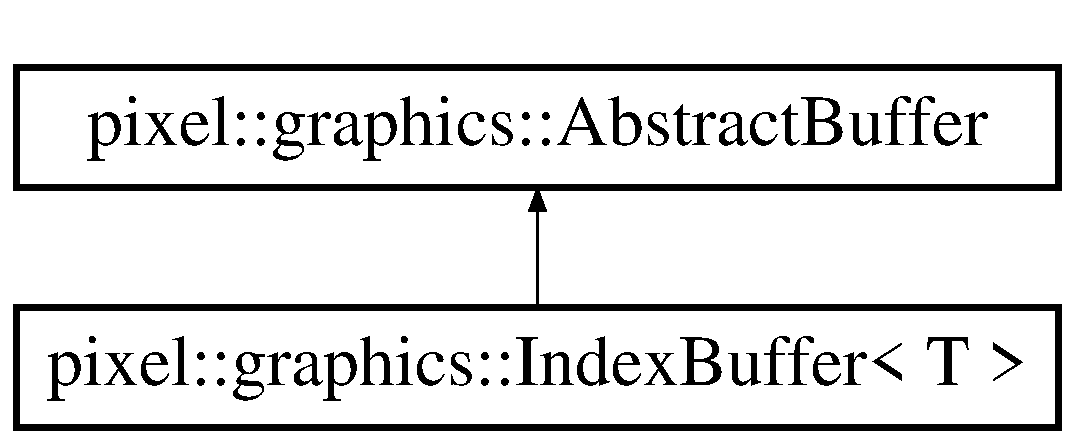
\includegraphics[height=2.000000cm]{classpixel_1_1graphics_1_1_index_buffer}
\end{center}
\end{figure}
\subsection*{Public Member Functions}
\begin{DoxyCompactItemize}
\item 
\hyperlink{classpixel_1_1graphics_1_1_index_buffer_ac5e5c987e447ff151b794a9b61940a29}{Index\+Buffer} ()
\item 
G\+Lenum \hyperlink{classpixel_1_1graphics_1_1_index_buffer_afd886afe46f7ec109902a4ff40ef2f24}{element\+Type} () const
\item 
void \hyperlink{classpixel_1_1graphics_1_1_index_buffer_aef55496774e132eb2deac595165e3576}{load\+Data} (const T $\ast$data, const int \hyperlink{namespacepixel_a465745e3b1a334686475c629948876f0}{size})
\item 
{\footnotesize template$<$size\+\_\+t length$>$ }\\void \hyperlink{classpixel_1_1graphics_1_1_index_buffer_a77168f7b0643fb6dd336108d2498eca9}{load} (std\+::array$<$ T, length $>$ data)
\item 
void \hyperlink{classpixel_1_1graphics_1_1_index_buffer_a70b8fdbdd19c8800e005425712426bde}{bind} () override
\item 
void \hyperlink{classpixel_1_1graphics_1_1_index_buffer_a5a90a44db73a048c76cf0fade5867621}{unbind} () override
\item 
G\+Luint \hyperlink{classpixel_1_1graphics_1_1_index_buffer_a6c02db9641270ccfbd77ddba3fc4e4d5}{buffer\+\_\+id} () const
\end{DoxyCompactItemize}
\subsection*{Private Attributes}
\begin{DoxyCompactItemize}
\item 
G\+Luint \hyperlink{classpixel_1_1graphics_1_1_index_buffer_a85ecce71a34c017da3d2f45d89a07d11}{buffer\+\_\+id\+\_\+} \{\}
\end{DoxyCompactItemize}


\subsection{Constructor \& Destructor Documentation}
\mbox{\Hypertarget{classpixel_1_1graphics_1_1_index_buffer_ac5e5c987e447ff151b794a9b61940a29}\label{classpixel_1_1graphics_1_1_index_buffer_ac5e5c987e447ff151b794a9b61940a29}} 
\index{pixel\+::graphics\+::\+Index\+Buffer@{pixel\+::graphics\+::\+Index\+Buffer}!Index\+Buffer@{Index\+Buffer}}
\index{Index\+Buffer@{Index\+Buffer}!pixel\+::graphics\+::\+Index\+Buffer@{pixel\+::graphics\+::\+Index\+Buffer}}
\subsubsection{\texorpdfstring{Index\+Buffer()}{IndexBuffer()}}
{\footnotesize\ttfamily template$<$typename T $>$ \\
\hyperlink{classpixel_1_1graphics_1_1_index_buffer}{pixel\+::graphics\+::\+Index\+Buffer}$<$ T $>$\+::\hyperlink{classpixel_1_1graphics_1_1_index_buffer}{Index\+Buffer} (\begin{DoxyParamCaption}{ }\end{DoxyParamCaption})}



\subsection{Member Function Documentation}
\mbox{\Hypertarget{classpixel_1_1graphics_1_1_index_buffer_a70b8fdbdd19c8800e005425712426bde}\label{classpixel_1_1graphics_1_1_index_buffer_a70b8fdbdd19c8800e005425712426bde}} 
\index{pixel\+::graphics\+::\+Index\+Buffer@{pixel\+::graphics\+::\+Index\+Buffer}!bind@{bind}}
\index{bind@{bind}!pixel\+::graphics\+::\+Index\+Buffer@{pixel\+::graphics\+::\+Index\+Buffer}}
\subsubsection{\texorpdfstring{bind()}{bind()}}
{\footnotesize\ttfamily template$<$typename T $>$ \\
void \hyperlink{classpixel_1_1graphics_1_1_index_buffer}{pixel\+::graphics\+::\+Index\+Buffer}$<$ T $>$\+::bind (\begin{DoxyParamCaption}{ }\end{DoxyParamCaption})\hspace{0.3cm}{\ttfamily [override]}, {\ttfamily [virtual]}}



Implements \hyperlink{classpixel_1_1graphics_1_1_abstract_buffer_a9d3bb463f35f08f5604012b7d22e113a}{pixel\+::graphics\+::\+Abstract\+Buffer}.

\mbox{\Hypertarget{classpixel_1_1graphics_1_1_index_buffer_a6c02db9641270ccfbd77ddba3fc4e4d5}\label{classpixel_1_1graphics_1_1_index_buffer_a6c02db9641270ccfbd77ddba3fc4e4d5}} 
\index{pixel\+::graphics\+::\+Index\+Buffer@{pixel\+::graphics\+::\+Index\+Buffer}!buffer\+\_\+id@{buffer\+\_\+id}}
\index{buffer\+\_\+id@{buffer\+\_\+id}!pixel\+::graphics\+::\+Index\+Buffer@{pixel\+::graphics\+::\+Index\+Buffer}}
\subsubsection{\texorpdfstring{buffer\+\_\+id()}{buffer\_id()}}
{\footnotesize\ttfamily template$<$typename T $>$ \\
G\+Luint \hyperlink{classpixel_1_1graphics_1_1_index_buffer}{pixel\+::graphics\+::\+Index\+Buffer}$<$ T $>$\+::buffer\+\_\+id (\begin{DoxyParamCaption}{ }\end{DoxyParamCaption}) const}

\mbox{\Hypertarget{classpixel_1_1graphics_1_1_index_buffer_afd886afe46f7ec109902a4ff40ef2f24}\label{classpixel_1_1graphics_1_1_index_buffer_afd886afe46f7ec109902a4ff40ef2f24}} 
\index{pixel\+::graphics\+::\+Index\+Buffer@{pixel\+::graphics\+::\+Index\+Buffer}!element\+Type@{element\+Type}}
\index{element\+Type@{element\+Type}!pixel\+::graphics\+::\+Index\+Buffer@{pixel\+::graphics\+::\+Index\+Buffer}}
\subsubsection{\texorpdfstring{element\+Type()}{elementType()}}
{\footnotesize\ttfamily template$<$typename T $>$ \\
G\+Lenum \hyperlink{classpixel_1_1graphics_1_1_index_buffer}{pixel\+::graphics\+::\+Index\+Buffer}$<$ T $>$\+::element\+Type (\begin{DoxyParamCaption}{ }\end{DoxyParamCaption}) const}

\mbox{\Hypertarget{classpixel_1_1graphics_1_1_index_buffer_a77168f7b0643fb6dd336108d2498eca9}\label{classpixel_1_1graphics_1_1_index_buffer_a77168f7b0643fb6dd336108d2498eca9}} 
\index{pixel\+::graphics\+::\+Index\+Buffer@{pixel\+::graphics\+::\+Index\+Buffer}!load@{load}}
\index{load@{load}!pixel\+::graphics\+::\+Index\+Buffer@{pixel\+::graphics\+::\+Index\+Buffer}}
\subsubsection{\texorpdfstring{load()}{load()}}
{\footnotesize\ttfamily template$<$typename T$>$ \\
template$<$size\+\_\+t length$>$ \\
void \hyperlink{classpixel_1_1graphics_1_1_index_buffer}{pixel\+::graphics\+::\+Index\+Buffer}$<$ T $>$\+::load (\begin{DoxyParamCaption}\item[{std\+::array$<$ T, length $>$}]{data }\end{DoxyParamCaption})}

\mbox{\Hypertarget{classpixel_1_1graphics_1_1_index_buffer_aef55496774e132eb2deac595165e3576}\label{classpixel_1_1graphics_1_1_index_buffer_aef55496774e132eb2deac595165e3576}} 
\index{pixel\+::graphics\+::\+Index\+Buffer@{pixel\+::graphics\+::\+Index\+Buffer}!load\+Data@{load\+Data}}
\index{load\+Data@{load\+Data}!pixel\+::graphics\+::\+Index\+Buffer@{pixel\+::graphics\+::\+Index\+Buffer}}
\subsubsection{\texorpdfstring{load\+Data()}{loadData()}}
{\footnotesize\ttfamily template$<$typename T$>$ \\
void \hyperlink{classpixel_1_1graphics_1_1_index_buffer}{pixel\+::graphics\+::\+Index\+Buffer}$<$ T $>$\+::load\+Data (\begin{DoxyParamCaption}\item[{const T $\ast$}]{data,  }\item[{const int}]{size }\end{DoxyParamCaption})}

\mbox{\Hypertarget{classpixel_1_1graphics_1_1_index_buffer_a5a90a44db73a048c76cf0fade5867621}\label{classpixel_1_1graphics_1_1_index_buffer_a5a90a44db73a048c76cf0fade5867621}} 
\index{pixel\+::graphics\+::\+Index\+Buffer@{pixel\+::graphics\+::\+Index\+Buffer}!unbind@{unbind}}
\index{unbind@{unbind}!pixel\+::graphics\+::\+Index\+Buffer@{pixel\+::graphics\+::\+Index\+Buffer}}
\subsubsection{\texorpdfstring{unbind()}{unbind()}}
{\footnotesize\ttfamily template$<$typename T $>$ \\
void \hyperlink{classpixel_1_1graphics_1_1_index_buffer}{pixel\+::graphics\+::\+Index\+Buffer}$<$ T $>$\+::unbind (\begin{DoxyParamCaption}{ }\end{DoxyParamCaption})\hspace{0.3cm}{\ttfamily [override]}, {\ttfamily [virtual]}}



Implements \hyperlink{classpixel_1_1graphics_1_1_abstract_buffer_aee49569fa5c1767a40f2371ec96e40fc}{pixel\+::graphics\+::\+Abstract\+Buffer}.



\subsection{Member Data Documentation}
\mbox{\Hypertarget{classpixel_1_1graphics_1_1_index_buffer_a85ecce71a34c017da3d2f45d89a07d11}\label{classpixel_1_1graphics_1_1_index_buffer_a85ecce71a34c017da3d2f45d89a07d11}} 
\index{pixel\+::graphics\+::\+Index\+Buffer@{pixel\+::graphics\+::\+Index\+Buffer}!buffer\+\_\+id\+\_\+@{buffer\+\_\+id\+\_\+}}
\index{buffer\+\_\+id\+\_\+@{buffer\+\_\+id\+\_\+}!pixel\+::graphics\+::\+Index\+Buffer@{pixel\+::graphics\+::\+Index\+Buffer}}
\subsubsection{\texorpdfstring{buffer\+\_\+id\+\_\+}{buffer\_id\_}}
{\footnotesize\ttfamily template$<$typename T$>$ \\
G\+Luint \hyperlink{classpixel_1_1graphics_1_1_index_buffer}{pixel\+::graphics\+::\+Index\+Buffer}$<$ T $>$\+::buffer\+\_\+id\+\_\+ \{\}\hspace{0.3cm}{\ttfamily [private]}}



The documentation for this class was generated from the following file\+:\begin{DoxyCompactItemize}
\item 
pixel/pixel/graphics/\hyperlink{buffer_8h}{buffer.\+h}\end{DoxyCompactItemize}

\hypertarget{classpixel_1_1input_1_1_keyboard}{}\section{pixel\+:\+:input\+:\+:Keyboard Class Reference}
\label{classpixel_1_1input_1_1_keyboard}\index{pixel\+::input\+::\+Keyboard@{pixel\+::input\+::\+Keyboard}}


{\ttfamily \#include $<$pixel/input/keyboard.\+h$>$}

\subsection*{Public Types}
\begin{DoxyCompactItemize}
\item 
using \hyperlink{classpixel_1_1input_1_1_keyboard_a9c2e61fefeba656cf2eb1adfccacc58a}{Keymap} = unordered\+\_\+map$<$ uint32\+\_\+t, bool $>$
\end{DoxyCompactItemize}
\subsection*{Public Member Functions}
\begin{DoxyCompactItemize}
\item 
\hyperlink{classpixel_1_1input_1_1_keyboard_a2604776e54e7511a26d0b1c7e03c44e2}{Keyboard} ()=default
\end{DoxyCompactItemize}
\subsection*{Static Public Member Functions}
\begin{DoxyCompactItemize}
\item 
static void \hyperlink{classpixel_1_1input_1_1_keyboard_abb0164a3125839568abc8447ac671a87}{register\+\_\+callback} (G\+L\+F\+Wwindow $\ast$window)
\item 
static void \hyperlink{classpixel_1_1input_1_1_keyboard_a56a80cab312b6241d368e77f07f1b126}{key\+\_\+callback} (G\+L\+F\+Wwindow $\ast$window, int key, int scancode, int action, int mods)
\item 
static void \hyperlink{classpixel_1_1input_1_1_keyboard_a5c220f10381043f8c784ce69f4ae6015}{clear\+\_\+keymap} ()
\end{DoxyCompactItemize}
\subsection*{Static Public Attributes}
\begin{DoxyCompactItemize}
\item 
static \hyperlink{classpixel_1_1input_1_1_keyboard_a9c2e61fefeba656cf2eb1adfccacc58a}{Keymap} \hyperlink{classpixel_1_1input_1_1_keyboard_ac0044c74f811cec7f45dd36038982725}{keymap} = \hyperlink{classpixel_1_1input_1_1_keyboard_a9c2e61fefeba656cf2eb1adfccacc58a}{Keyboard\+::\+Keymap}()
\end{DoxyCompactItemize}


\subsection{Member Typedef Documentation}
\mbox{\Hypertarget{classpixel_1_1input_1_1_keyboard_a9c2e61fefeba656cf2eb1adfccacc58a}\label{classpixel_1_1input_1_1_keyboard_a9c2e61fefeba656cf2eb1adfccacc58a}} 
\index{pixel\+::input\+::\+Keyboard@{pixel\+::input\+::\+Keyboard}!Keymap@{Keymap}}
\index{Keymap@{Keymap}!pixel\+::input\+::\+Keyboard@{pixel\+::input\+::\+Keyboard}}
\subsubsection{\texorpdfstring{Keymap}{Keymap}}
{\footnotesize\ttfamily using \hyperlink{classpixel_1_1input_1_1_keyboard_a9c2e61fefeba656cf2eb1adfccacc58a}{pixel\+::input\+::\+Keyboard\+::\+Keymap} =  unordered\+\_\+map$<$uint32\+\_\+t, bool$>$}



\subsection{Constructor \& Destructor Documentation}
\mbox{\Hypertarget{classpixel_1_1input_1_1_keyboard_a2604776e54e7511a26d0b1c7e03c44e2}\label{classpixel_1_1input_1_1_keyboard_a2604776e54e7511a26d0b1c7e03c44e2}} 
\index{pixel\+::input\+::\+Keyboard@{pixel\+::input\+::\+Keyboard}!Keyboard@{Keyboard}}
\index{Keyboard@{Keyboard}!pixel\+::input\+::\+Keyboard@{pixel\+::input\+::\+Keyboard}}
\subsubsection{\texorpdfstring{Keyboard()}{Keyboard()}}
{\footnotesize\ttfamily pixel\+::input\+::\+Keyboard\+::\+Keyboard (\begin{DoxyParamCaption}{ }\end{DoxyParamCaption})\hspace{0.3cm}{\ttfamily [default]}}



\subsection{Member Function Documentation}
\mbox{\Hypertarget{classpixel_1_1input_1_1_keyboard_a5c220f10381043f8c784ce69f4ae6015}\label{classpixel_1_1input_1_1_keyboard_a5c220f10381043f8c784ce69f4ae6015}} 
\index{pixel\+::input\+::\+Keyboard@{pixel\+::input\+::\+Keyboard}!clear\+\_\+keymap@{clear\+\_\+keymap}}
\index{clear\+\_\+keymap@{clear\+\_\+keymap}!pixel\+::input\+::\+Keyboard@{pixel\+::input\+::\+Keyboard}}
\subsubsection{\texorpdfstring{clear\+\_\+keymap()}{clear\_keymap()}}
{\footnotesize\ttfamily void pixel\+::input\+::\+Keyboard\+::clear\+\_\+keymap (\begin{DoxyParamCaption}{ }\end{DoxyParamCaption})\hspace{0.3cm}{\ttfamily [static]}}

\mbox{\Hypertarget{classpixel_1_1input_1_1_keyboard_a56a80cab312b6241d368e77f07f1b126}\label{classpixel_1_1input_1_1_keyboard_a56a80cab312b6241d368e77f07f1b126}} 
\index{pixel\+::input\+::\+Keyboard@{pixel\+::input\+::\+Keyboard}!key\+\_\+callback@{key\+\_\+callback}}
\index{key\+\_\+callback@{key\+\_\+callback}!pixel\+::input\+::\+Keyboard@{pixel\+::input\+::\+Keyboard}}
\subsubsection{\texorpdfstring{key\+\_\+callback()}{key\_callback()}}
{\footnotesize\ttfamily void pixel\+::input\+::\+Keyboard\+::key\+\_\+callback (\begin{DoxyParamCaption}\item[{G\+L\+F\+Wwindow $\ast$}]{window,  }\item[{int}]{key,  }\item[{int}]{scancode,  }\item[{int}]{action,  }\item[{int}]{mods }\end{DoxyParamCaption})\hspace{0.3cm}{\ttfamily [static]}}

\mbox{\Hypertarget{classpixel_1_1input_1_1_keyboard_abb0164a3125839568abc8447ac671a87}\label{classpixel_1_1input_1_1_keyboard_abb0164a3125839568abc8447ac671a87}} 
\index{pixel\+::input\+::\+Keyboard@{pixel\+::input\+::\+Keyboard}!register\+\_\+callback@{register\+\_\+callback}}
\index{register\+\_\+callback@{register\+\_\+callback}!pixel\+::input\+::\+Keyboard@{pixel\+::input\+::\+Keyboard}}
\subsubsection{\texorpdfstring{register\+\_\+callback()}{register\_callback()}}
{\footnotesize\ttfamily void pixel\+::input\+::\+Keyboard\+::register\+\_\+callback (\begin{DoxyParamCaption}\item[{G\+L\+F\+Wwindow $\ast$}]{window }\end{DoxyParamCaption})\hspace{0.3cm}{\ttfamily [static]}}



\subsection{Member Data Documentation}
\mbox{\Hypertarget{classpixel_1_1input_1_1_keyboard_ac0044c74f811cec7f45dd36038982725}\label{classpixel_1_1input_1_1_keyboard_ac0044c74f811cec7f45dd36038982725}} 
\index{pixel\+::input\+::\+Keyboard@{pixel\+::input\+::\+Keyboard}!keymap@{keymap}}
\index{keymap@{keymap}!pixel\+::input\+::\+Keyboard@{pixel\+::input\+::\+Keyboard}}
\subsubsection{\texorpdfstring{keymap}{keymap}}
{\footnotesize\ttfamily \hyperlink{classpixel_1_1input_1_1_keyboard_a9c2e61fefeba656cf2eb1adfccacc58a}{Keyboard\+::\+Keymap} pixel\+::input\+::\+Keyboard\+::keymap = \hyperlink{classpixel_1_1input_1_1_keyboard_a9c2e61fefeba656cf2eb1adfccacc58a}{Keyboard\+::\+Keymap}()\hspace{0.3cm}{\ttfamily [static]}}



The documentation for this class was generated from the following files\+:\begin{DoxyCompactItemize}
\item 
pixel/pixel/input/\hyperlink{keyboard_8h}{keyboard.\+h}\item 
pixel/pixel/input/\hyperlink{keyboard_8cpp}{keyboard.\+cpp}\end{DoxyCompactItemize}

\hypertarget{struct_layout}{}\section{Layout Struct Reference}
\label{struct_layout}\index{Layout@{Layout}}
\subsection*{Public Member Functions}
\begin{DoxyCompactItemize}
\item 
\hyperlink{struct_layout_a1239c2d12968bcfd073571e91e01f30a}{Layout} (const \hyperlink{structpixel_1_1graphics_1_1_attribute}{Attribute} \&attr)
\end{DoxyCompactItemize}
\subsection*{Public Attributes}
\begin{DoxyCompactItemize}
\item 
int \hyperlink{struct_layout_a7f928bc38185dc8527b16f2dd35191cf}{base\+Location}
\item 
int \hyperlink{struct_layout_a483e349db82792cfbd393797c2396957}{location\+Span}
\item 
int \hyperlink{struct_layout_a143bf56c3c9785cc75e2360dbe818e84}{size}
\item 
G\+Lenum \hyperlink{struct_layout_a039d56a72da89806f7019c12c8ab3ea7}{type}
\end{DoxyCompactItemize}


\subsection{Constructor \& Destructor Documentation}
\mbox{\Hypertarget{struct_layout_a1239c2d12968bcfd073571e91e01f30a}\label{struct_layout_a1239c2d12968bcfd073571e91e01f30a}} 
\index{Layout@{Layout}!Layout@{Layout}}
\index{Layout@{Layout}!Layout@{Layout}}
\subsubsection{\texorpdfstring{Layout()}{Layout()}}
{\footnotesize\ttfamily Layout\+::\+Layout (\begin{DoxyParamCaption}\item[{const \hyperlink{structpixel_1_1graphics_1_1_attribute}{Attribute} \&}]{attr }\end{DoxyParamCaption})\hspace{0.3cm}{\ttfamily [explicit]}}



\subsection{Member Data Documentation}
\mbox{\Hypertarget{struct_layout_a7f928bc38185dc8527b16f2dd35191cf}\label{struct_layout_a7f928bc38185dc8527b16f2dd35191cf}} 
\index{Layout@{Layout}!base\+Location@{base\+Location}}
\index{base\+Location@{base\+Location}!Layout@{Layout}}
\subsubsection{\texorpdfstring{base\+Location}{baseLocation}}
{\footnotesize\ttfamily int Layout\+::base\+Location}

\mbox{\Hypertarget{struct_layout_a483e349db82792cfbd393797c2396957}\label{struct_layout_a483e349db82792cfbd393797c2396957}} 
\index{Layout@{Layout}!location\+Span@{location\+Span}}
\index{location\+Span@{location\+Span}!Layout@{Layout}}
\subsubsection{\texorpdfstring{location\+Span}{locationSpan}}
{\footnotesize\ttfamily int Layout\+::location\+Span}

\mbox{\Hypertarget{struct_layout_a143bf56c3c9785cc75e2360dbe818e84}\label{struct_layout_a143bf56c3c9785cc75e2360dbe818e84}} 
\index{Layout@{Layout}!size@{size}}
\index{size@{size}!Layout@{Layout}}
\subsubsection{\texorpdfstring{size}{size}}
{\footnotesize\ttfamily int Layout\+::size}

\mbox{\Hypertarget{struct_layout_a039d56a72da89806f7019c12c8ab3ea7}\label{struct_layout_a039d56a72da89806f7019c12c8ab3ea7}} 
\index{Layout@{Layout}!type@{type}}
\index{type@{type}!Layout@{Layout}}
\subsubsection{\texorpdfstring{type}{type}}
{\footnotesize\ttfamily G\+Lenum Layout\+::type}



The documentation for this struct was generated from the following file\+:\begin{DoxyCompactItemize}
\item 
pixel/pixel/graphics/\hyperlink{buffer_8cpp}{buffer.\+cpp}\end{DoxyCompactItemize}

\hypertarget{classpixel_1_1renderers_1_1_line_renderer}{}\section{pixel\+:\+:renderers\+:\+:Line\+Renderer Class Reference}
\label{classpixel_1_1renderers_1_1_line_renderer}\index{pixel\+::renderers\+::\+Line\+Renderer@{pixel\+::renderers\+::\+Line\+Renderer}}


{\ttfamily \#include $<$pixel/renderers/line\+\_\+renderer.\+h$>$}

\subsection*{Public Member Functions}
\begin{DoxyCompactItemize}
\item 
\hyperlink{classpixel_1_1renderers_1_1_line_renderer_adf08d52089304ffbcdb6430b4d40c241}{Line\+Renderer} ()
\item 
void \hyperlink{classpixel_1_1renderers_1_1_line_renderer_a1980b5f5590d1f2c13d83db2551d819d}{render} (const vector$<$ \hyperlink{classpixel_1_1_line_segment}{Line\+Segment} $>$ \&, const \hyperlink{classpixel_1_1graphics_1_1_camera}{Camera} \&)
\end{DoxyCompactItemize}
\subsection*{Private Attributes}
\begin{DoxyCompactItemize}
\item 
\hyperlink{classpixel_1_1graphics_1_1_shader}{Shader} \hyperlink{classpixel_1_1renderers_1_1_line_renderer_a6a2758421a2ee6e249d78deb3a8d6ca2}{shader\+\_\+}
\item 
\hyperlink{classpixel_1_1graphics_1_1_vao}{Vao} \hyperlink{classpixel_1_1renderers_1_1_line_renderer_aaa62d25c3b7c62156a4c90053f6a659e}{vao\+\_\+}
\end{DoxyCompactItemize}


\subsection{Constructor \& Destructor Documentation}
\mbox{\Hypertarget{classpixel_1_1renderers_1_1_line_renderer_adf08d52089304ffbcdb6430b4d40c241}\label{classpixel_1_1renderers_1_1_line_renderer_adf08d52089304ffbcdb6430b4d40c241}} 
\index{pixel\+::renderers\+::\+Line\+Renderer@{pixel\+::renderers\+::\+Line\+Renderer}!Line\+Renderer@{Line\+Renderer}}
\index{Line\+Renderer@{Line\+Renderer}!pixel\+::renderers\+::\+Line\+Renderer@{pixel\+::renderers\+::\+Line\+Renderer}}
\subsubsection{\texorpdfstring{Line\+Renderer()}{LineRenderer()}}
{\footnotesize\ttfamily pixel\+::renderers\+::\+Line\+Renderer\+::\+Line\+Renderer (\begin{DoxyParamCaption}{ }\end{DoxyParamCaption})}



\subsection{Member Function Documentation}
\mbox{\Hypertarget{classpixel_1_1renderers_1_1_line_renderer_a1980b5f5590d1f2c13d83db2551d819d}\label{classpixel_1_1renderers_1_1_line_renderer_a1980b5f5590d1f2c13d83db2551d819d}} 
\index{pixel\+::renderers\+::\+Line\+Renderer@{pixel\+::renderers\+::\+Line\+Renderer}!render@{render}}
\index{render@{render}!pixel\+::renderers\+::\+Line\+Renderer@{pixel\+::renderers\+::\+Line\+Renderer}}
\subsubsection{\texorpdfstring{render()}{render()}}
{\footnotesize\ttfamily void pixel\+::renderers\+::\+Line\+Renderer\+::render (\begin{DoxyParamCaption}\item[{const vector$<$ \hyperlink{classpixel_1_1_line_segment}{Line\+Segment} $>$ \&}]{line\+\_\+segments,  }\item[{const \hyperlink{classpixel_1_1graphics_1_1_camera}{Camera} \&}]{camera }\end{DoxyParamCaption})}



\subsection{Member Data Documentation}
\mbox{\Hypertarget{classpixel_1_1renderers_1_1_line_renderer_a6a2758421a2ee6e249d78deb3a8d6ca2}\label{classpixel_1_1renderers_1_1_line_renderer_a6a2758421a2ee6e249d78deb3a8d6ca2}} 
\index{pixel\+::renderers\+::\+Line\+Renderer@{pixel\+::renderers\+::\+Line\+Renderer}!shader\+\_\+@{shader\+\_\+}}
\index{shader\+\_\+@{shader\+\_\+}!pixel\+::renderers\+::\+Line\+Renderer@{pixel\+::renderers\+::\+Line\+Renderer}}
\subsubsection{\texorpdfstring{shader\+\_\+}{shader\_}}
{\footnotesize\ttfamily \hyperlink{classpixel_1_1graphics_1_1_shader}{Shader} pixel\+::renderers\+::\+Line\+Renderer\+::shader\+\_\+\hspace{0.3cm}{\ttfamily [private]}}

\mbox{\Hypertarget{classpixel_1_1renderers_1_1_line_renderer_aaa62d25c3b7c62156a4c90053f6a659e}\label{classpixel_1_1renderers_1_1_line_renderer_aaa62d25c3b7c62156a4c90053f6a659e}} 
\index{pixel\+::renderers\+::\+Line\+Renderer@{pixel\+::renderers\+::\+Line\+Renderer}!vao\+\_\+@{vao\+\_\+}}
\index{vao\+\_\+@{vao\+\_\+}!pixel\+::renderers\+::\+Line\+Renderer@{pixel\+::renderers\+::\+Line\+Renderer}}
\subsubsection{\texorpdfstring{vao\+\_\+}{vao\_}}
{\footnotesize\ttfamily \hyperlink{classpixel_1_1graphics_1_1_vao}{Vao} pixel\+::renderers\+::\+Line\+Renderer\+::vao\+\_\+\hspace{0.3cm}{\ttfamily [private]}}



The documentation for this class was generated from the following files\+:\begin{DoxyCompactItemize}
\item 
pixel/pixel/renderers/\hyperlink{line__renderer_8h}{line\+\_\+renderer.\+h}\item 
pixel/pixel/renderers/\hyperlink{line__renderer_8cpp}{line\+\_\+renderer.\+cpp}\end{DoxyCompactItemize}

\hypertarget{classpixel_1_1_line_segment}{}\section{pixel\+:\+:Line\+Segment Class Reference}
\label{classpixel_1_1_line_segment}\index{pixel\+::\+Line\+Segment@{pixel\+::\+Line\+Segment}}


{\ttfamily \#include $<$pixel/types.\+h$>$}

\subsection*{Public Member Functions}
\begin{DoxyCompactItemize}
\item 
\hyperlink{classpixel_1_1_line_segment_a0ad3d24c8192c89774e7caf277168d39}{Line\+Segment} ()=default
\item 
\hyperlink{classpixel_1_1_line_segment_a908ff0ace1fa46fa4ddc23d0f4413b18}{Line\+Segment} (float \hyperlink{classpixel_1_1_line_segment_a8471e97168d448505467cd0049131f1e}{x0}, float \hyperlink{classpixel_1_1_line_segment_a2d293acfc87ca0d41cb4926482160b6e}{y0}, float \hyperlink{classpixel_1_1_line_segment_a24f7b4c5d7ed1c256e852260beac619d}{x1}, float \hyperlink{classpixel_1_1_line_segment_ac28bac5789bed7818e6500378e16d97f}{y1})
\item 
float \hyperlink{classpixel_1_1_line_segment_ad3bac4aae966e09f98586c47f70dee44}{length} ()
\end{DoxyCompactItemize}
\subsection*{Public Attributes}
\begin{DoxyCompactItemize}
\item 
float \hyperlink{classpixel_1_1_line_segment_a8471e97168d448505467cd0049131f1e}{x0}
\item 
float \hyperlink{classpixel_1_1_line_segment_a2d293acfc87ca0d41cb4926482160b6e}{y0}
\item 
float \hyperlink{classpixel_1_1_line_segment_a24f7b4c5d7ed1c256e852260beac619d}{x1}
\item 
float \hyperlink{classpixel_1_1_line_segment_ac28bac5789bed7818e6500378e16d97f}{y1}
\end{DoxyCompactItemize}


\subsection{Constructor \& Destructor Documentation}
\mbox{\Hypertarget{classpixel_1_1_line_segment_a0ad3d24c8192c89774e7caf277168d39}\label{classpixel_1_1_line_segment_a0ad3d24c8192c89774e7caf277168d39}} 
\index{pixel\+::\+Line\+Segment@{pixel\+::\+Line\+Segment}!Line\+Segment@{Line\+Segment}}
\index{Line\+Segment@{Line\+Segment}!pixel\+::\+Line\+Segment@{pixel\+::\+Line\+Segment}}
\subsubsection{\texorpdfstring{Line\+Segment()}{LineSegment()}\hspace{0.1cm}{\footnotesize\ttfamily [1/2]}}
{\footnotesize\ttfamily pixel\+::\+Line\+Segment\+::\+Line\+Segment (\begin{DoxyParamCaption}{ }\end{DoxyParamCaption})\hspace{0.3cm}{\ttfamily [default]}}

\mbox{\Hypertarget{classpixel_1_1_line_segment_a908ff0ace1fa46fa4ddc23d0f4413b18}\label{classpixel_1_1_line_segment_a908ff0ace1fa46fa4ddc23d0f4413b18}} 
\index{pixel\+::\+Line\+Segment@{pixel\+::\+Line\+Segment}!Line\+Segment@{Line\+Segment}}
\index{Line\+Segment@{Line\+Segment}!pixel\+::\+Line\+Segment@{pixel\+::\+Line\+Segment}}
\subsubsection{\texorpdfstring{Line\+Segment()}{LineSegment()}\hspace{0.1cm}{\footnotesize\ttfamily [2/2]}}
{\footnotesize\ttfamily pixel\+::\+Line\+Segment\+::\+Line\+Segment (\begin{DoxyParamCaption}\item[{float}]{x0,  }\item[{float}]{y0,  }\item[{float}]{x1,  }\item[{float}]{y1 }\end{DoxyParamCaption})\hspace{0.3cm}{\ttfamily [inline]}}



\subsection{Member Function Documentation}
\mbox{\Hypertarget{classpixel_1_1_line_segment_ad3bac4aae966e09f98586c47f70dee44}\label{classpixel_1_1_line_segment_ad3bac4aae966e09f98586c47f70dee44}} 
\index{pixel\+::\+Line\+Segment@{pixel\+::\+Line\+Segment}!length@{length}}
\index{length@{length}!pixel\+::\+Line\+Segment@{pixel\+::\+Line\+Segment}}
\subsubsection{\texorpdfstring{length()}{length()}}
{\footnotesize\ttfamily float pixel\+::\+Line\+Segment\+::length (\begin{DoxyParamCaption}{ }\end{DoxyParamCaption})\hspace{0.3cm}{\ttfamily [inline]}}



\subsection{Member Data Documentation}
\mbox{\Hypertarget{classpixel_1_1_line_segment_a8471e97168d448505467cd0049131f1e}\label{classpixel_1_1_line_segment_a8471e97168d448505467cd0049131f1e}} 
\index{pixel\+::\+Line\+Segment@{pixel\+::\+Line\+Segment}!x0@{x0}}
\index{x0@{x0}!pixel\+::\+Line\+Segment@{pixel\+::\+Line\+Segment}}
\subsubsection{\texorpdfstring{x0}{x0}}
{\footnotesize\ttfamily float pixel\+::\+Line\+Segment\+::x0}

\mbox{\Hypertarget{classpixel_1_1_line_segment_a24f7b4c5d7ed1c256e852260beac619d}\label{classpixel_1_1_line_segment_a24f7b4c5d7ed1c256e852260beac619d}} 
\index{pixel\+::\+Line\+Segment@{pixel\+::\+Line\+Segment}!x1@{x1}}
\index{x1@{x1}!pixel\+::\+Line\+Segment@{pixel\+::\+Line\+Segment}}
\subsubsection{\texorpdfstring{x1}{x1}}
{\footnotesize\ttfamily float pixel\+::\+Line\+Segment\+::x1}

\mbox{\Hypertarget{classpixel_1_1_line_segment_a2d293acfc87ca0d41cb4926482160b6e}\label{classpixel_1_1_line_segment_a2d293acfc87ca0d41cb4926482160b6e}} 
\index{pixel\+::\+Line\+Segment@{pixel\+::\+Line\+Segment}!y0@{y0}}
\index{y0@{y0}!pixel\+::\+Line\+Segment@{pixel\+::\+Line\+Segment}}
\subsubsection{\texorpdfstring{y0}{y0}}
{\footnotesize\ttfamily float pixel\+::\+Line\+Segment\+::y0}

\mbox{\Hypertarget{classpixel_1_1_line_segment_ac28bac5789bed7818e6500378e16d97f}\label{classpixel_1_1_line_segment_ac28bac5789bed7818e6500378e16d97f}} 
\index{pixel\+::\+Line\+Segment@{pixel\+::\+Line\+Segment}!y1@{y1}}
\index{y1@{y1}!pixel\+::\+Line\+Segment@{pixel\+::\+Line\+Segment}}
\subsubsection{\texorpdfstring{y1}{y1}}
{\footnotesize\ttfamily float pixel\+::\+Line\+Segment\+::y1}



The documentation for this class was generated from the following file\+:\begin{DoxyCompactItemize}
\item 
pixel/pixel/\hyperlink{types_8h}{types.\+h}\end{DoxyCompactItemize}

\hypertarget{classpixel_1_1graphics_1_1_offscreen_render_target}{}\section{pixel\+:\+:graphics\+:\+:Offscreen\+Render\+Target Class Reference}
\label{classpixel_1_1graphics_1_1_offscreen_render_target}\index{pixel\+::graphics\+::\+Offscreen\+Render\+Target@{pixel\+::graphics\+::\+Offscreen\+Render\+Target}}


{\ttfamily \#include $<$pixel/graphics/offscreen\+\_\+render\+\_\+target.\+h$>$}

\subsection*{Public Member Functions}
\begin{DoxyCompactItemize}
\item 
\hyperlink{classpixel_1_1graphics_1_1_offscreen_render_target_a09267c820dd5d349a0a455f8d38d442a}{Offscreen\+Render\+Target} ()
\item 
void \hyperlink{classpixel_1_1graphics_1_1_offscreen_render_target_a1ef8c7558df5d0defc1dd7083641d436}{activate} ()
\item 
void \hyperlink{classpixel_1_1graphics_1_1_offscreen_render_target_af4578733da935ecefd9d8e00032ff59c}{deactivate} ()
\item 
void \hyperlink{classpixel_1_1graphics_1_1_offscreen_render_target_a498298c152b939eda03742fde96507c9}{draw} (const glm\+::ivec4 \&draw\+\_\+region)
\item 
glm\+::ivec2 \hyperlink{classpixel_1_1graphics_1_1_offscreen_render_target_a146e78904b9f8ea9df00a141b17ac8b0}{window\+\_\+size} () const
\item 
void \hyperlink{classpixel_1_1graphics_1_1_offscreen_render_target_a47f5ea45b79659e2601e8f7ccc063c37}{set\+\_\+window\+\_\+size} (const glm\+::ivec2 \&)
\item 
void \hyperlink{classpixel_1_1graphics_1_1_offscreen_render_target_a1cfaa54b19e2f12fe839e95e947bb92c}{set\+\_\+window\+\_\+size} (int, int)
\end{DoxyCompactItemize}
\subsection*{Private Member Functions}
\begin{DoxyCompactItemize}
\item 
void \hyperlink{classpixel_1_1graphics_1_1_offscreen_render_target_a60bdb5799fc903d63922e63a873274af}{resize\+\_\+buffers} (unsigned int width, unsigned int height)
\item 
void \hyperlink{classpixel_1_1graphics_1_1_offscreen_render_target_acac4df8b179a089d8672ad5b84c1a27a}{attach\+\_\+buffers} ()
\end{DoxyCompactItemize}
\subsection*{Private Attributes}
\begin{DoxyCompactItemize}
\item 
unsigned \hyperlink{classpixel_1_1graphics_1_1_offscreen_render_target_ab040cfa6c283593124e05bf2e668176a}{fbo\+\_\+}
\item 
unsigned \hyperlink{classpixel_1_1graphics_1_1_offscreen_render_target_a4ad6892135a7e4f68953944c287c2645}{rbo\+\_\+color\+\_\+}
\item 
unsigned \hyperlink{classpixel_1_1graphics_1_1_offscreen_render_target_a862be1d24be8b6a08132e36796d46085}{rbo\+\_\+depth\+\_\+stencil\+\_\+}
\item 
glm\+::ivec2 \hyperlink{classpixel_1_1graphics_1_1_offscreen_render_target_a583e64f23f20f404fd3f845e2d0e207d}{size\+\_\+}
\item 
glm\+::ivec4 \hyperlink{classpixel_1_1graphics_1_1_offscreen_render_target_a47407823935b91e47783db5a381691c4}{old\+\_\+viewport\+\_\+}
\end{DoxyCompactItemize}


\subsection{Constructor \& Destructor Documentation}
\mbox{\Hypertarget{classpixel_1_1graphics_1_1_offscreen_render_target_a09267c820dd5d349a0a455f8d38d442a}\label{classpixel_1_1graphics_1_1_offscreen_render_target_a09267c820dd5d349a0a455f8d38d442a}} 
\index{pixel\+::graphics\+::\+Offscreen\+Render\+Target@{pixel\+::graphics\+::\+Offscreen\+Render\+Target}!Offscreen\+Render\+Target@{Offscreen\+Render\+Target}}
\index{Offscreen\+Render\+Target@{Offscreen\+Render\+Target}!pixel\+::graphics\+::\+Offscreen\+Render\+Target@{pixel\+::graphics\+::\+Offscreen\+Render\+Target}}
\subsubsection{\texorpdfstring{Offscreen\+Render\+Target()}{OffscreenRenderTarget()}}
{\footnotesize\ttfamily pixel\+::graphics\+::\+Offscreen\+Render\+Target\+::\+Offscreen\+Render\+Target (\begin{DoxyParamCaption}{ }\end{DoxyParamCaption})}



\subsection{Member Function Documentation}
\mbox{\Hypertarget{classpixel_1_1graphics_1_1_offscreen_render_target_a1ef8c7558df5d0defc1dd7083641d436}\label{classpixel_1_1graphics_1_1_offscreen_render_target_a1ef8c7558df5d0defc1dd7083641d436}} 
\index{pixel\+::graphics\+::\+Offscreen\+Render\+Target@{pixel\+::graphics\+::\+Offscreen\+Render\+Target}!activate@{activate}}
\index{activate@{activate}!pixel\+::graphics\+::\+Offscreen\+Render\+Target@{pixel\+::graphics\+::\+Offscreen\+Render\+Target}}
\subsubsection{\texorpdfstring{activate()}{activate()}}
{\footnotesize\ttfamily void pixel\+::graphics\+::\+Offscreen\+Render\+Target\+::activate (\begin{DoxyParamCaption}{ }\end{DoxyParamCaption})}

\mbox{\Hypertarget{classpixel_1_1graphics_1_1_offscreen_render_target_acac4df8b179a089d8672ad5b84c1a27a}\label{classpixel_1_1graphics_1_1_offscreen_render_target_acac4df8b179a089d8672ad5b84c1a27a}} 
\index{pixel\+::graphics\+::\+Offscreen\+Render\+Target@{pixel\+::graphics\+::\+Offscreen\+Render\+Target}!attach\+\_\+buffers@{attach\+\_\+buffers}}
\index{attach\+\_\+buffers@{attach\+\_\+buffers}!pixel\+::graphics\+::\+Offscreen\+Render\+Target@{pixel\+::graphics\+::\+Offscreen\+Render\+Target}}
\subsubsection{\texorpdfstring{attach\+\_\+buffers()}{attach\_buffers()}}
{\footnotesize\ttfamily void pixel\+::graphics\+::\+Offscreen\+Render\+Target\+::attach\+\_\+buffers (\begin{DoxyParamCaption}{ }\end{DoxyParamCaption})\hspace{0.3cm}{\ttfamily [private]}}

\mbox{\Hypertarget{classpixel_1_1graphics_1_1_offscreen_render_target_af4578733da935ecefd9d8e00032ff59c}\label{classpixel_1_1graphics_1_1_offscreen_render_target_af4578733da935ecefd9d8e00032ff59c}} 
\index{pixel\+::graphics\+::\+Offscreen\+Render\+Target@{pixel\+::graphics\+::\+Offscreen\+Render\+Target}!deactivate@{deactivate}}
\index{deactivate@{deactivate}!pixel\+::graphics\+::\+Offscreen\+Render\+Target@{pixel\+::graphics\+::\+Offscreen\+Render\+Target}}
\subsubsection{\texorpdfstring{deactivate()}{deactivate()}}
{\footnotesize\ttfamily void pixel\+::graphics\+::\+Offscreen\+Render\+Target\+::deactivate (\begin{DoxyParamCaption}{ }\end{DoxyParamCaption})}

\mbox{\Hypertarget{classpixel_1_1graphics_1_1_offscreen_render_target_a498298c152b939eda03742fde96507c9}\label{classpixel_1_1graphics_1_1_offscreen_render_target_a498298c152b939eda03742fde96507c9}} 
\index{pixel\+::graphics\+::\+Offscreen\+Render\+Target@{pixel\+::graphics\+::\+Offscreen\+Render\+Target}!draw@{draw}}
\index{draw@{draw}!pixel\+::graphics\+::\+Offscreen\+Render\+Target@{pixel\+::graphics\+::\+Offscreen\+Render\+Target}}
\subsubsection{\texorpdfstring{draw()}{draw()}}
{\footnotesize\ttfamily void pixel\+::graphics\+::\+Offscreen\+Render\+Target\+::draw (\begin{DoxyParamCaption}\item[{const glm\+::ivec4 \&}]{draw\+\_\+region }\end{DoxyParamCaption})}

\mbox{\Hypertarget{classpixel_1_1graphics_1_1_offscreen_render_target_a60bdb5799fc903d63922e63a873274af}\label{classpixel_1_1graphics_1_1_offscreen_render_target_a60bdb5799fc903d63922e63a873274af}} 
\index{pixel\+::graphics\+::\+Offscreen\+Render\+Target@{pixel\+::graphics\+::\+Offscreen\+Render\+Target}!resize\+\_\+buffers@{resize\+\_\+buffers}}
\index{resize\+\_\+buffers@{resize\+\_\+buffers}!pixel\+::graphics\+::\+Offscreen\+Render\+Target@{pixel\+::graphics\+::\+Offscreen\+Render\+Target}}
\subsubsection{\texorpdfstring{resize\+\_\+buffers()}{resize\_buffers()}}
{\footnotesize\ttfamily void pixel\+::graphics\+::\+Offscreen\+Render\+Target\+::resize\+\_\+buffers (\begin{DoxyParamCaption}\item[{unsigned int}]{width,  }\item[{unsigned int}]{height }\end{DoxyParamCaption})\hspace{0.3cm}{\ttfamily [private]}}

\mbox{\Hypertarget{classpixel_1_1graphics_1_1_offscreen_render_target_a47f5ea45b79659e2601e8f7ccc063c37}\label{classpixel_1_1graphics_1_1_offscreen_render_target_a47f5ea45b79659e2601e8f7ccc063c37}} 
\index{pixel\+::graphics\+::\+Offscreen\+Render\+Target@{pixel\+::graphics\+::\+Offscreen\+Render\+Target}!set\+\_\+window\+\_\+size@{set\+\_\+window\+\_\+size}}
\index{set\+\_\+window\+\_\+size@{set\+\_\+window\+\_\+size}!pixel\+::graphics\+::\+Offscreen\+Render\+Target@{pixel\+::graphics\+::\+Offscreen\+Render\+Target}}
\subsubsection{\texorpdfstring{set\+\_\+window\+\_\+size()}{set\_window\_size()}\hspace{0.1cm}{\footnotesize\ttfamily [1/2]}}
{\footnotesize\ttfamily void pixel\+::graphics\+::\+Offscreen\+Render\+Target\+::set\+\_\+window\+\_\+size (\begin{DoxyParamCaption}\item[{const glm\+::ivec2 \&}]{v }\end{DoxyParamCaption})}

\mbox{\Hypertarget{classpixel_1_1graphics_1_1_offscreen_render_target_a1cfaa54b19e2f12fe839e95e947bb92c}\label{classpixel_1_1graphics_1_1_offscreen_render_target_a1cfaa54b19e2f12fe839e95e947bb92c}} 
\index{pixel\+::graphics\+::\+Offscreen\+Render\+Target@{pixel\+::graphics\+::\+Offscreen\+Render\+Target}!set\+\_\+window\+\_\+size@{set\+\_\+window\+\_\+size}}
\index{set\+\_\+window\+\_\+size@{set\+\_\+window\+\_\+size}!pixel\+::graphics\+::\+Offscreen\+Render\+Target@{pixel\+::graphics\+::\+Offscreen\+Render\+Target}}
\subsubsection{\texorpdfstring{set\+\_\+window\+\_\+size()}{set\_window\_size()}\hspace{0.1cm}{\footnotesize\ttfamily [2/2]}}
{\footnotesize\ttfamily void pixel\+::graphics\+::\+Offscreen\+Render\+Target\+::set\+\_\+window\+\_\+size (\begin{DoxyParamCaption}\item[{int}]{w,  }\item[{int}]{h }\end{DoxyParamCaption})}

\mbox{\Hypertarget{classpixel_1_1graphics_1_1_offscreen_render_target_a146e78904b9f8ea9df00a141b17ac8b0}\label{classpixel_1_1graphics_1_1_offscreen_render_target_a146e78904b9f8ea9df00a141b17ac8b0}} 
\index{pixel\+::graphics\+::\+Offscreen\+Render\+Target@{pixel\+::graphics\+::\+Offscreen\+Render\+Target}!window\+\_\+size@{window\+\_\+size}}
\index{window\+\_\+size@{window\+\_\+size}!pixel\+::graphics\+::\+Offscreen\+Render\+Target@{pixel\+::graphics\+::\+Offscreen\+Render\+Target}}
\subsubsection{\texorpdfstring{window\+\_\+size()}{window\_size()}}
{\footnotesize\ttfamily glm\+::ivec2 pixel\+::graphics\+::\+Offscreen\+Render\+Target\+::window\+\_\+size (\begin{DoxyParamCaption}{ }\end{DoxyParamCaption}) const}



\subsection{Member Data Documentation}
\mbox{\Hypertarget{classpixel_1_1graphics_1_1_offscreen_render_target_ab040cfa6c283593124e05bf2e668176a}\label{classpixel_1_1graphics_1_1_offscreen_render_target_ab040cfa6c283593124e05bf2e668176a}} 
\index{pixel\+::graphics\+::\+Offscreen\+Render\+Target@{pixel\+::graphics\+::\+Offscreen\+Render\+Target}!fbo\+\_\+@{fbo\+\_\+}}
\index{fbo\+\_\+@{fbo\+\_\+}!pixel\+::graphics\+::\+Offscreen\+Render\+Target@{pixel\+::graphics\+::\+Offscreen\+Render\+Target}}
\subsubsection{\texorpdfstring{fbo\+\_\+}{fbo\_}}
{\footnotesize\ttfamily unsigned pixel\+::graphics\+::\+Offscreen\+Render\+Target\+::fbo\+\_\+\hspace{0.3cm}{\ttfamily [private]}}

\mbox{\Hypertarget{classpixel_1_1graphics_1_1_offscreen_render_target_a47407823935b91e47783db5a381691c4}\label{classpixel_1_1graphics_1_1_offscreen_render_target_a47407823935b91e47783db5a381691c4}} 
\index{pixel\+::graphics\+::\+Offscreen\+Render\+Target@{pixel\+::graphics\+::\+Offscreen\+Render\+Target}!old\+\_\+viewport\+\_\+@{old\+\_\+viewport\+\_\+}}
\index{old\+\_\+viewport\+\_\+@{old\+\_\+viewport\+\_\+}!pixel\+::graphics\+::\+Offscreen\+Render\+Target@{pixel\+::graphics\+::\+Offscreen\+Render\+Target}}
\subsubsection{\texorpdfstring{old\+\_\+viewport\+\_\+}{old\_viewport\_}}
{\footnotesize\ttfamily glm\+::ivec4 pixel\+::graphics\+::\+Offscreen\+Render\+Target\+::old\+\_\+viewport\+\_\+\hspace{0.3cm}{\ttfamily [private]}}

\mbox{\Hypertarget{classpixel_1_1graphics_1_1_offscreen_render_target_a4ad6892135a7e4f68953944c287c2645}\label{classpixel_1_1graphics_1_1_offscreen_render_target_a4ad6892135a7e4f68953944c287c2645}} 
\index{pixel\+::graphics\+::\+Offscreen\+Render\+Target@{pixel\+::graphics\+::\+Offscreen\+Render\+Target}!rbo\+\_\+color\+\_\+@{rbo\+\_\+color\+\_\+}}
\index{rbo\+\_\+color\+\_\+@{rbo\+\_\+color\+\_\+}!pixel\+::graphics\+::\+Offscreen\+Render\+Target@{pixel\+::graphics\+::\+Offscreen\+Render\+Target}}
\subsubsection{\texorpdfstring{rbo\+\_\+color\+\_\+}{rbo\_color\_}}
{\footnotesize\ttfamily unsigned pixel\+::graphics\+::\+Offscreen\+Render\+Target\+::rbo\+\_\+color\+\_\+\hspace{0.3cm}{\ttfamily [private]}}

\mbox{\Hypertarget{classpixel_1_1graphics_1_1_offscreen_render_target_a862be1d24be8b6a08132e36796d46085}\label{classpixel_1_1graphics_1_1_offscreen_render_target_a862be1d24be8b6a08132e36796d46085}} 
\index{pixel\+::graphics\+::\+Offscreen\+Render\+Target@{pixel\+::graphics\+::\+Offscreen\+Render\+Target}!rbo\+\_\+depth\+\_\+stencil\+\_\+@{rbo\+\_\+depth\+\_\+stencil\+\_\+}}
\index{rbo\+\_\+depth\+\_\+stencil\+\_\+@{rbo\+\_\+depth\+\_\+stencil\+\_\+}!pixel\+::graphics\+::\+Offscreen\+Render\+Target@{pixel\+::graphics\+::\+Offscreen\+Render\+Target}}
\subsubsection{\texorpdfstring{rbo\+\_\+depth\+\_\+stencil\+\_\+}{rbo\_depth\_stencil\_}}
{\footnotesize\ttfamily unsigned pixel\+::graphics\+::\+Offscreen\+Render\+Target\+::rbo\+\_\+depth\+\_\+stencil\+\_\+\hspace{0.3cm}{\ttfamily [private]}}

\mbox{\Hypertarget{classpixel_1_1graphics_1_1_offscreen_render_target_a583e64f23f20f404fd3f845e2d0e207d}\label{classpixel_1_1graphics_1_1_offscreen_render_target_a583e64f23f20f404fd3f845e2d0e207d}} 
\index{pixel\+::graphics\+::\+Offscreen\+Render\+Target@{pixel\+::graphics\+::\+Offscreen\+Render\+Target}!size\+\_\+@{size\+\_\+}}
\index{size\+\_\+@{size\+\_\+}!pixel\+::graphics\+::\+Offscreen\+Render\+Target@{pixel\+::graphics\+::\+Offscreen\+Render\+Target}}
\subsubsection{\texorpdfstring{size\+\_\+}{size\_}}
{\footnotesize\ttfamily glm\+::ivec2 pixel\+::graphics\+::\+Offscreen\+Render\+Target\+::size\+\_\+\hspace{0.3cm}{\ttfamily [private]}}



The documentation for this class was generated from the following files\+:\begin{DoxyCompactItemize}
\item 
pixel/pixel/graphics/\hyperlink{offscreen__render__target_8h}{offscreen\+\_\+render\+\_\+target.\+h}\item 
pixel/pixel/graphics/\hyperlink{offscreen__render__target_8cpp}{offscreen\+\_\+render\+\_\+target.\+cpp}\end{DoxyCompactItemize}

\hypertarget{structpixel_1_1pack_1_1_pack_node}{}\section{pixel\+:\+:pack\+:\+:Pack\+Node Struct Reference}
\label{structpixel_1_1pack_1_1_pack_node}\index{pixel\+::pack\+::\+Pack\+Node@{pixel\+::pack\+::\+Pack\+Node}}


{\ttfamily \#include $<$pixel/graphics/pack.\+h$>$}

\subsection*{Public Member Functions}
\begin{DoxyCompactItemize}
\item 
\hyperlink{structpixel_1_1pack_1_1_pack_node_aa878a4442b6d942b8f7fc83e75244dcd}{Pack\+Node} (unsigned \hyperlink{structpixel_1_1pack_1_1_pack_node_a6354ce26408343f8285102c6457e2ad0}{x}, unsigned \hyperlink{structpixel_1_1pack_1_1_pack_node_a5f7655b61750b69345416a77ee2138cb}{y}, unsigned \hyperlink{structpixel_1_1pack_1_1_pack_node_af54e70dd691d64ac8696dc353a53de72}{w}, unsigned \hyperlink{structpixel_1_1pack_1_1_pack_node_a380024626a85cde82d459a86e79c7651}{h})
\item 
\hyperlink{structpixel_1_1pack_1_1_pack_node_a8b2fde54fe2e46cc591f46e77b2fd0ad}{Pack\+Node} ()=default
\item 
\hyperlink{structpixel_1_1pack_1_1_pack_node_a8ce9fffbc415ea9509106959c99421fc}{$\sim$\+Pack\+Node} ()
\item 
bool \hyperlink{structpixel_1_1pack_1_1_pack_node_a106addb740c67e52ea781ecbfb778d22}{can\+\_\+fit} (unsigned \+\_\+w, unsigned \+\_\+h)
\item 
bool \hyperlink{structpixel_1_1pack_1_1_pack_node_a6c8bdca8866f0a2e19c9a9f2a65cff38}{should\+\_\+flip} (unsigned \+\_\+w, unsigned \+\_\+h)
\end{DoxyCompactItemize}
\subsection*{Public Attributes}
\begin{DoxyCompactItemize}
\item 
unsigned \hyperlink{structpixel_1_1pack_1_1_pack_node_af54e70dd691d64ac8696dc353a53de72}{w} \{\}
\item 
unsigned \hyperlink{structpixel_1_1pack_1_1_pack_node_a380024626a85cde82d459a86e79c7651}{h} \{\}
\item 
unsigned \hyperlink{structpixel_1_1pack_1_1_pack_node_a6354ce26408343f8285102c6457e2ad0}{x} \{\}
\item 
unsigned \hyperlink{structpixel_1_1pack_1_1_pack_node_a5f7655b61750b69345416a77ee2138cb}{y} \{\}
\item 
bool \hyperlink{structpixel_1_1pack_1_1_pack_node_ac15528125c21b185065569689f65a76f}{used} \{false\}
\item 
bool \hyperlink{structpixel_1_1pack_1_1_pack_node_ae718b2584684e9b08e76d8619674d301}{flipped} \{false\}
\item 
\hyperlink{structpixel_1_1pack_1_1_pack_node}{Pack\+Node} $\ast$ \hyperlink{structpixel_1_1pack_1_1_pack_node_a3622911c5c2374af970989dff1cb8485}{right} \{nullptr\}
\item 
\hyperlink{structpixel_1_1pack_1_1_pack_node}{Pack\+Node} $\ast$ \hyperlink{structpixel_1_1pack_1_1_pack_node_a21d64fe74713de90912922f7aff1c768}{down} \{nullptr\}
\end{DoxyCompactItemize}


\subsection{Constructor \& Destructor Documentation}
\mbox{\Hypertarget{structpixel_1_1pack_1_1_pack_node_aa878a4442b6d942b8f7fc83e75244dcd}\label{structpixel_1_1pack_1_1_pack_node_aa878a4442b6d942b8f7fc83e75244dcd}} 
\index{pixel\+::pack\+::\+Pack\+Node@{pixel\+::pack\+::\+Pack\+Node}!Pack\+Node@{Pack\+Node}}
\index{Pack\+Node@{Pack\+Node}!pixel\+::pack\+::\+Pack\+Node@{pixel\+::pack\+::\+Pack\+Node}}
\subsubsection{\texorpdfstring{Pack\+Node()}{PackNode()}\hspace{0.1cm}{\footnotesize\ttfamily [1/2]}}
{\footnotesize\ttfamily pixel\+::pack\+::\+Pack\+Node\+::\+Pack\+Node (\begin{DoxyParamCaption}\item[{unsigned}]{x,  }\item[{unsigned}]{y,  }\item[{unsigned}]{w,  }\item[{unsigned}]{h }\end{DoxyParamCaption})\hspace{0.3cm}{\ttfamily [inline]}}

\mbox{\Hypertarget{structpixel_1_1pack_1_1_pack_node_a8b2fde54fe2e46cc591f46e77b2fd0ad}\label{structpixel_1_1pack_1_1_pack_node_a8b2fde54fe2e46cc591f46e77b2fd0ad}} 
\index{pixel\+::pack\+::\+Pack\+Node@{pixel\+::pack\+::\+Pack\+Node}!Pack\+Node@{Pack\+Node}}
\index{Pack\+Node@{Pack\+Node}!pixel\+::pack\+::\+Pack\+Node@{pixel\+::pack\+::\+Pack\+Node}}
\subsubsection{\texorpdfstring{Pack\+Node()}{PackNode()}\hspace{0.1cm}{\footnotesize\ttfamily [2/2]}}
{\footnotesize\ttfamily pixel\+::pack\+::\+Pack\+Node\+::\+Pack\+Node (\begin{DoxyParamCaption}{ }\end{DoxyParamCaption})\hspace{0.3cm}{\ttfamily [default]}}

\mbox{\Hypertarget{structpixel_1_1pack_1_1_pack_node_a8ce9fffbc415ea9509106959c99421fc}\label{structpixel_1_1pack_1_1_pack_node_a8ce9fffbc415ea9509106959c99421fc}} 
\index{pixel\+::pack\+::\+Pack\+Node@{pixel\+::pack\+::\+Pack\+Node}!````~Pack\+Node@{$\sim$\+Pack\+Node}}
\index{````~Pack\+Node@{$\sim$\+Pack\+Node}!pixel\+::pack\+::\+Pack\+Node@{pixel\+::pack\+::\+Pack\+Node}}
\subsubsection{\texorpdfstring{$\sim$\+Pack\+Node()}{~PackNode()}}
{\footnotesize\ttfamily pixel\+::pack\+::\+Pack\+Node\+::$\sim$\+Pack\+Node (\begin{DoxyParamCaption}{ }\end{DoxyParamCaption})\hspace{0.3cm}{\ttfamily [inline]}}



\subsection{Member Function Documentation}
\mbox{\Hypertarget{structpixel_1_1pack_1_1_pack_node_a106addb740c67e52ea781ecbfb778d22}\label{structpixel_1_1pack_1_1_pack_node_a106addb740c67e52ea781ecbfb778d22}} 
\index{pixel\+::pack\+::\+Pack\+Node@{pixel\+::pack\+::\+Pack\+Node}!can\+\_\+fit@{can\+\_\+fit}}
\index{can\+\_\+fit@{can\+\_\+fit}!pixel\+::pack\+::\+Pack\+Node@{pixel\+::pack\+::\+Pack\+Node}}
\subsubsection{\texorpdfstring{can\+\_\+fit()}{can\_fit()}}
{\footnotesize\ttfamily bool pixel\+::pack\+::\+Pack\+Node\+::can\+\_\+fit (\begin{DoxyParamCaption}\item[{unsigned}]{\+\_\+w,  }\item[{unsigned}]{\+\_\+h }\end{DoxyParamCaption})\hspace{0.3cm}{\ttfamily [inline]}}

\mbox{\Hypertarget{structpixel_1_1pack_1_1_pack_node_a6c8bdca8866f0a2e19c9a9f2a65cff38}\label{structpixel_1_1pack_1_1_pack_node_a6c8bdca8866f0a2e19c9a9f2a65cff38}} 
\index{pixel\+::pack\+::\+Pack\+Node@{pixel\+::pack\+::\+Pack\+Node}!should\+\_\+flip@{should\+\_\+flip}}
\index{should\+\_\+flip@{should\+\_\+flip}!pixel\+::pack\+::\+Pack\+Node@{pixel\+::pack\+::\+Pack\+Node}}
\subsubsection{\texorpdfstring{should\+\_\+flip()}{should\_flip()}}
{\footnotesize\ttfamily bool pixel\+::pack\+::\+Pack\+Node\+::should\+\_\+flip (\begin{DoxyParamCaption}\item[{unsigned}]{\+\_\+w,  }\item[{unsigned}]{\+\_\+h }\end{DoxyParamCaption})\hspace{0.3cm}{\ttfamily [inline]}}



\subsection{Member Data Documentation}
\mbox{\Hypertarget{structpixel_1_1pack_1_1_pack_node_a21d64fe74713de90912922f7aff1c768}\label{structpixel_1_1pack_1_1_pack_node_a21d64fe74713de90912922f7aff1c768}} 
\index{pixel\+::pack\+::\+Pack\+Node@{pixel\+::pack\+::\+Pack\+Node}!down@{down}}
\index{down@{down}!pixel\+::pack\+::\+Pack\+Node@{pixel\+::pack\+::\+Pack\+Node}}
\subsubsection{\texorpdfstring{down}{down}}
{\footnotesize\ttfamily \hyperlink{structpixel_1_1pack_1_1_pack_node}{Pack\+Node}$\ast$ pixel\+::pack\+::\+Pack\+Node\+::down \{nullptr\}}

\mbox{\Hypertarget{structpixel_1_1pack_1_1_pack_node_ae718b2584684e9b08e76d8619674d301}\label{structpixel_1_1pack_1_1_pack_node_ae718b2584684e9b08e76d8619674d301}} 
\index{pixel\+::pack\+::\+Pack\+Node@{pixel\+::pack\+::\+Pack\+Node}!flipped@{flipped}}
\index{flipped@{flipped}!pixel\+::pack\+::\+Pack\+Node@{pixel\+::pack\+::\+Pack\+Node}}
\subsubsection{\texorpdfstring{flipped}{flipped}}
{\footnotesize\ttfamily bool pixel\+::pack\+::\+Pack\+Node\+::flipped \{false\}}

\mbox{\Hypertarget{structpixel_1_1pack_1_1_pack_node_a380024626a85cde82d459a86e79c7651}\label{structpixel_1_1pack_1_1_pack_node_a380024626a85cde82d459a86e79c7651}} 
\index{pixel\+::pack\+::\+Pack\+Node@{pixel\+::pack\+::\+Pack\+Node}!h@{h}}
\index{h@{h}!pixel\+::pack\+::\+Pack\+Node@{pixel\+::pack\+::\+Pack\+Node}}
\subsubsection{\texorpdfstring{h}{h}}
{\footnotesize\ttfamily unsigned pixel\+::pack\+::\+Pack\+Node\+::h \{\}}

\mbox{\Hypertarget{structpixel_1_1pack_1_1_pack_node_a3622911c5c2374af970989dff1cb8485}\label{structpixel_1_1pack_1_1_pack_node_a3622911c5c2374af970989dff1cb8485}} 
\index{pixel\+::pack\+::\+Pack\+Node@{pixel\+::pack\+::\+Pack\+Node}!right@{right}}
\index{right@{right}!pixel\+::pack\+::\+Pack\+Node@{pixel\+::pack\+::\+Pack\+Node}}
\subsubsection{\texorpdfstring{right}{right}}
{\footnotesize\ttfamily \hyperlink{structpixel_1_1pack_1_1_pack_node}{Pack\+Node}$\ast$ pixel\+::pack\+::\+Pack\+Node\+::right \{nullptr\}}

\mbox{\Hypertarget{structpixel_1_1pack_1_1_pack_node_ac15528125c21b185065569689f65a76f}\label{structpixel_1_1pack_1_1_pack_node_ac15528125c21b185065569689f65a76f}} 
\index{pixel\+::pack\+::\+Pack\+Node@{pixel\+::pack\+::\+Pack\+Node}!used@{used}}
\index{used@{used}!pixel\+::pack\+::\+Pack\+Node@{pixel\+::pack\+::\+Pack\+Node}}
\subsubsection{\texorpdfstring{used}{used}}
{\footnotesize\ttfamily bool pixel\+::pack\+::\+Pack\+Node\+::used \{false\}}

\mbox{\Hypertarget{structpixel_1_1pack_1_1_pack_node_af54e70dd691d64ac8696dc353a53de72}\label{structpixel_1_1pack_1_1_pack_node_af54e70dd691d64ac8696dc353a53de72}} 
\index{pixel\+::pack\+::\+Pack\+Node@{pixel\+::pack\+::\+Pack\+Node}!w@{w}}
\index{w@{w}!pixel\+::pack\+::\+Pack\+Node@{pixel\+::pack\+::\+Pack\+Node}}
\subsubsection{\texorpdfstring{w}{w}}
{\footnotesize\ttfamily unsigned pixel\+::pack\+::\+Pack\+Node\+::w \{\}}

\mbox{\Hypertarget{structpixel_1_1pack_1_1_pack_node_a6354ce26408343f8285102c6457e2ad0}\label{structpixel_1_1pack_1_1_pack_node_a6354ce26408343f8285102c6457e2ad0}} 
\index{pixel\+::pack\+::\+Pack\+Node@{pixel\+::pack\+::\+Pack\+Node}!x@{x}}
\index{x@{x}!pixel\+::pack\+::\+Pack\+Node@{pixel\+::pack\+::\+Pack\+Node}}
\subsubsection{\texorpdfstring{x}{x}}
{\footnotesize\ttfamily unsigned pixel\+::pack\+::\+Pack\+Node\+::x \{\}}

\mbox{\Hypertarget{structpixel_1_1pack_1_1_pack_node_a5f7655b61750b69345416a77ee2138cb}\label{structpixel_1_1pack_1_1_pack_node_a5f7655b61750b69345416a77ee2138cb}} 
\index{pixel\+::pack\+::\+Pack\+Node@{pixel\+::pack\+::\+Pack\+Node}!y@{y}}
\index{y@{y}!pixel\+::pack\+::\+Pack\+Node@{pixel\+::pack\+::\+Pack\+Node}}
\subsubsection{\texorpdfstring{y}{y}}
{\footnotesize\ttfamily unsigned pixel\+::pack\+::\+Pack\+Node\+::y \{\}}



The documentation for this struct was generated from the following file\+:\begin{DoxyCompactItemize}
\item 
pixel/pixel/graphics/\hyperlink{pack_8h}{pack.\+h}\end{DoxyCompactItemize}

\hypertarget{structpixel_1_1pack_1_1_pack_params}{}\section{pixel\+:\+:pack\+:\+:Pack\+Params Struct Reference}
\label{structpixel_1_1pack_1_1_pack_params}\index{pixel\+::pack\+::\+Pack\+Params@{pixel\+::pack\+::\+Pack\+Params}}


{\ttfamily \#include $<$pixel/graphics/pack.\+h$>$}

\subsection*{Public Member Functions}
\begin{DoxyCompactItemize}
\item 
\hyperlink{structpixel_1_1pack_1_1_pack_params_a980b508c330947788993092d9f786fb3}{Pack\+Params} ()=default
\item 
\hyperlink{structpixel_1_1pack_1_1_pack_params_ae4c64428986269e6ea9c78c69939a840}{Pack\+Params} (unsigned \hyperlink{structpixel_1_1pack_1_1_pack_params_ad785be2d851bd17b013bd7ac9841e275}{x}, unsigned \hyperlink{structpixel_1_1pack_1_1_pack_params_a7f2d379f827c491805b245777515af21}{y}, unsigned \hyperlink{structpixel_1_1pack_1_1_pack_params_ae77b5bfda6eba8f7b56d80c045d1b8ab}{z}, bool \hyperlink{structpixel_1_1pack_1_1_pack_params_a36e94201bd65095fed383599f2b50ac3}{flipped})
\end{DoxyCompactItemize}
\subsection*{Public Attributes}
\begin{DoxyCompactItemize}
\item 
unsigned \hyperlink{structpixel_1_1pack_1_1_pack_params_ad785be2d851bd17b013bd7ac9841e275}{x} \{\}
\item 
unsigned \hyperlink{structpixel_1_1pack_1_1_pack_params_a7f2d379f827c491805b245777515af21}{y} \{\}
\item 
unsigned \hyperlink{structpixel_1_1pack_1_1_pack_params_ae77b5bfda6eba8f7b56d80c045d1b8ab}{z} \{\}
\item 
bool \hyperlink{structpixel_1_1pack_1_1_pack_params_a36e94201bd65095fed383599f2b50ac3}{flipped}
\end{DoxyCompactItemize}


\subsection{Constructor \& Destructor Documentation}
\mbox{\Hypertarget{structpixel_1_1pack_1_1_pack_params_a980b508c330947788993092d9f786fb3}\label{structpixel_1_1pack_1_1_pack_params_a980b508c330947788993092d9f786fb3}} 
\index{pixel\+::pack\+::\+Pack\+Params@{pixel\+::pack\+::\+Pack\+Params}!Pack\+Params@{Pack\+Params}}
\index{Pack\+Params@{Pack\+Params}!pixel\+::pack\+::\+Pack\+Params@{pixel\+::pack\+::\+Pack\+Params}}
\subsubsection{\texorpdfstring{Pack\+Params()}{PackParams()}\hspace{0.1cm}{\footnotesize\ttfamily [1/2]}}
{\footnotesize\ttfamily pixel\+::pack\+::\+Pack\+Params\+::\+Pack\+Params (\begin{DoxyParamCaption}{ }\end{DoxyParamCaption})\hspace{0.3cm}{\ttfamily [default]}}

\mbox{\Hypertarget{structpixel_1_1pack_1_1_pack_params_ae4c64428986269e6ea9c78c69939a840}\label{structpixel_1_1pack_1_1_pack_params_ae4c64428986269e6ea9c78c69939a840}} 
\index{pixel\+::pack\+::\+Pack\+Params@{pixel\+::pack\+::\+Pack\+Params}!Pack\+Params@{Pack\+Params}}
\index{Pack\+Params@{Pack\+Params}!pixel\+::pack\+::\+Pack\+Params@{pixel\+::pack\+::\+Pack\+Params}}
\subsubsection{\texorpdfstring{Pack\+Params()}{PackParams()}\hspace{0.1cm}{\footnotesize\ttfamily [2/2]}}
{\footnotesize\ttfamily pixel\+::pack\+::\+Pack\+Params\+::\+Pack\+Params (\begin{DoxyParamCaption}\item[{unsigned}]{x,  }\item[{unsigned}]{y,  }\item[{unsigned}]{z,  }\item[{bool}]{flipped }\end{DoxyParamCaption})\hspace{0.3cm}{\ttfamily [inline]}}



\subsection{Member Data Documentation}
\mbox{\Hypertarget{structpixel_1_1pack_1_1_pack_params_a36e94201bd65095fed383599f2b50ac3}\label{structpixel_1_1pack_1_1_pack_params_a36e94201bd65095fed383599f2b50ac3}} 
\index{pixel\+::pack\+::\+Pack\+Params@{pixel\+::pack\+::\+Pack\+Params}!flipped@{flipped}}
\index{flipped@{flipped}!pixel\+::pack\+::\+Pack\+Params@{pixel\+::pack\+::\+Pack\+Params}}
\subsubsection{\texorpdfstring{flipped}{flipped}}
{\footnotesize\ttfamily bool pixel\+::pack\+::\+Pack\+Params\+::flipped}

\mbox{\Hypertarget{structpixel_1_1pack_1_1_pack_params_ad785be2d851bd17b013bd7ac9841e275}\label{structpixel_1_1pack_1_1_pack_params_ad785be2d851bd17b013bd7ac9841e275}} 
\index{pixel\+::pack\+::\+Pack\+Params@{pixel\+::pack\+::\+Pack\+Params}!x@{x}}
\index{x@{x}!pixel\+::pack\+::\+Pack\+Params@{pixel\+::pack\+::\+Pack\+Params}}
\subsubsection{\texorpdfstring{x}{x}}
{\footnotesize\ttfamily unsigned pixel\+::pack\+::\+Pack\+Params\+::x \{\}}

\mbox{\Hypertarget{structpixel_1_1pack_1_1_pack_params_a7f2d379f827c491805b245777515af21}\label{structpixel_1_1pack_1_1_pack_params_a7f2d379f827c491805b245777515af21}} 
\index{pixel\+::pack\+::\+Pack\+Params@{pixel\+::pack\+::\+Pack\+Params}!y@{y}}
\index{y@{y}!pixel\+::pack\+::\+Pack\+Params@{pixel\+::pack\+::\+Pack\+Params}}
\subsubsection{\texorpdfstring{y}{y}}
{\footnotesize\ttfamily unsigned pixel\+::pack\+::\+Pack\+Params\+::y \{\}}

\mbox{\Hypertarget{structpixel_1_1pack_1_1_pack_params_ae77b5bfda6eba8f7b56d80c045d1b8ab}\label{structpixel_1_1pack_1_1_pack_params_ae77b5bfda6eba8f7b56d80c045d1b8ab}} 
\index{pixel\+::pack\+::\+Pack\+Params@{pixel\+::pack\+::\+Pack\+Params}!z@{z}}
\index{z@{z}!pixel\+::pack\+::\+Pack\+Params@{pixel\+::pack\+::\+Pack\+Params}}
\subsubsection{\texorpdfstring{z}{z}}
{\footnotesize\ttfamily unsigned pixel\+::pack\+::\+Pack\+Params\+::z \{\}}



The documentation for this struct was generated from the following file\+:\begin{DoxyCompactItemize}
\item 
pixel/pixel/graphics/\hyperlink{pack_8h}{pack.\+h}\end{DoxyCompactItemize}

\hypertarget{structpixel_1_1_tile_layer_1_1_properties}{}\section{pixel\+:\+:Tile\+Layer\+:\+:Properties Struct Reference}
\label{structpixel_1_1_tile_layer_1_1_properties}\index{pixel\+::\+Tile\+Layer\+::\+Properties@{pixel\+::\+Tile\+Layer\+::\+Properties}}


{\ttfamily \#include $<$pixel/tilemap/tile\+\_\+layer.\+h$>$}

\subsection*{Public Attributes}
\begin{DoxyCompactItemize}
\item 
uint32\+\_\+t \hyperlink{structpixel_1_1_tile_layer_1_1_properties_a67fcb4eb4b6b041324a08ec2aa8ef3f7}{flags}
\item 
uint8\+\_\+t $\ast$ \hyperlink{structpixel_1_1_tile_layer_1_1_properties_a9bad1a071416a7eacb80b7079f3c889b}{height\+\_\+map}
\end{DoxyCompactItemize}


\subsection{Member Data Documentation}
\mbox{\Hypertarget{structpixel_1_1_tile_layer_1_1_properties_a67fcb4eb4b6b041324a08ec2aa8ef3f7}\label{structpixel_1_1_tile_layer_1_1_properties_a67fcb4eb4b6b041324a08ec2aa8ef3f7}} 
\index{pixel\+::\+Tile\+Layer\+::\+Properties@{pixel\+::\+Tile\+Layer\+::\+Properties}!flags@{flags}}
\index{flags@{flags}!pixel\+::\+Tile\+Layer\+::\+Properties@{pixel\+::\+Tile\+Layer\+::\+Properties}}
\subsubsection{\texorpdfstring{flags}{flags}}
{\footnotesize\ttfamily uint32\+\_\+t pixel\+::\+Tile\+Layer\+::\+Properties\+::flags}

\mbox{\Hypertarget{structpixel_1_1_tile_layer_1_1_properties_a9bad1a071416a7eacb80b7079f3c889b}\label{structpixel_1_1_tile_layer_1_1_properties_a9bad1a071416a7eacb80b7079f3c889b}} 
\index{pixel\+::\+Tile\+Layer\+::\+Properties@{pixel\+::\+Tile\+Layer\+::\+Properties}!height\+\_\+map@{height\+\_\+map}}
\index{height\+\_\+map@{height\+\_\+map}!pixel\+::\+Tile\+Layer\+::\+Properties@{pixel\+::\+Tile\+Layer\+::\+Properties}}
\subsubsection{\texorpdfstring{height\+\_\+map}{height\_map}}
{\footnotesize\ttfamily uint8\+\_\+t$\ast$ pixel\+::\+Tile\+Layer\+::\+Properties\+::height\+\_\+map}



The documentation for this struct was generated from the following file\+:\begin{DoxyCompactItemize}
\item 
pixel/pixel/tilemap/\hyperlink{tile__layer_8h}{tile\+\_\+layer.\+h}\end{DoxyCompactItemize}

\hypertarget{classpixel_1_1_property_collection}{}\section{pixel\+:\+:Property\+Collection Class Reference}
\label{classpixel_1_1_property_collection}\index{pixel\+::\+Property\+Collection@{pixel\+::\+Property\+Collection}}
\subsection*{Public Member Functions}
\begin{DoxyCompactItemize}
\item 
\hyperlink{classpixel_1_1_property_collection_a9f122a6f3ad8409b781a2e18b5ad45a9}{Property\+Collection} (const vector$<$ tmx\+::\+Property $>$ \&props)
\item 
float \hyperlink{classpixel_1_1_property_collection_a076152a8f28cb9a1955c3fef8fed1e95}{get\+Float} (const string \&k)
\item 
float \hyperlink{classpixel_1_1_property_collection_a552df806ee1afa23d748b876c19a52f8}{get\+Float} (const string \&k, float default\+\_\+val)
\end{DoxyCompactItemize}
\subsection*{Private Attributes}
\begin{DoxyCompactItemize}
\item 
unordered\+\_\+map$<$ string, tmx\+::\+Property $>$ \hyperlink{classpixel_1_1_property_collection_add80655d2ec83c818d96dc88d56463dc}{props\+\_\+}
\end{DoxyCompactItemize}


\subsection{Constructor \& Destructor Documentation}
\mbox{\Hypertarget{classpixel_1_1_property_collection_a9f122a6f3ad8409b781a2e18b5ad45a9}\label{classpixel_1_1_property_collection_a9f122a6f3ad8409b781a2e18b5ad45a9}} 
\index{pixel\+::\+Property\+Collection@{pixel\+::\+Property\+Collection}!Property\+Collection@{Property\+Collection}}
\index{Property\+Collection@{Property\+Collection}!pixel\+::\+Property\+Collection@{pixel\+::\+Property\+Collection}}
\subsubsection{\texorpdfstring{Property\+Collection()}{PropertyCollection()}}
{\footnotesize\ttfamily pixel\+::\+Property\+Collection\+::\+Property\+Collection (\begin{DoxyParamCaption}\item[{const vector$<$ tmx\+::\+Property $>$ \&}]{props }\end{DoxyParamCaption})\hspace{0.3cm}{\ttfamily [inline]}}



\subsection{Member Function Documentation}
\mbox{\Hypertarget{classpixel_1_1_property_collection_a076152a8f28cb9a1955c3fef8fed1e95}\label{classpixel_1_1_property_collection_a076152a8f28cb9a1955c3fef8fed1e95}} 
\index{pixel\+::\+Property\+Collection@{pixel\+::\+Property\+Collection}!get\+Float@{get\+Float}}
\index{get\+Float@{get\+Float}!pixel\+::\+Property\+Collection@{pixel\+::\+Property\+Collection}}
\subsubsection{\texorpdfstring{get\+Float()}{getFloat()}\hspace{0.1cm}{\footnotesize\ttfamily [1/2]}}
{\footnotesize\ttfamily float pixel\+::\+Property\+Collection\+::get\+Float (\begin{DoxyParamCaption}\item[{const string \&}]{k }\end{DoxyParamCaption})\hspace{0.3cm}{\ttfamily [inline]}}

\mbox{\Hypertarget{classpixel_1_1_property_collection_a552df806ee1afa23d748b876c19a52f8}\label{classpixel_1_1_property_collection_a552df806ee1afa23d748b876c19a52f8}} 
\index{pixel\+::\+Property\+Collection@{pixel\+::\+Property\+Collection}!get\+Float@{get\+Float}}
\index{get\+Float@{get\+Float}!pixel\+::\+Property\+Collection@{pixel\+::\+Property\+Collection}}
\subsubsection{\texorpdfstring{get\+Float()}{getFloat()}\hspace{0.1cm}{\footnotesize\ttfamily [2/2]}}
{\footnotesize\ttfamily float pixel\+::\+Property\+Collection\+::get\+Float (\begin{DoxyParamCaption}\item[{const string \&}]{k,  }\item[{float}]{default\+\_\+val }\end{DoxyParamCaption})\hspace{0.3cm}{\ttfamily [inline]}}



\subsection{Member Data Documentation}
\mbox{\Hypertarget{classpixel_1_1_property_collection_add80655d2ec83c818d96dc88d56463dc}\label{classpixel_1_1_property_collection_add80655d2ec83c818d96dc88d56463dc}} 
\index{pixel\+::\+Property\+Collection@{pixel\+::\+Property\+Collection}!props\+\_\+@{props\+\_\+}}
\index{props\+\_\+@{props\+\_\+}!pixel\+::\+Property\+Collection@{pixel\+::\+Property\+Collection}}
\subsubsection{\texorpdfstring{props\+\_\+}{props\_}}
{\footnotesize\ttfamily unordered\+\_\+map$<$string, tmx\+::\+Property$>$ pixel\+::\+Property\+Collection\+::props\+\_\+\hspace{0.3cm}{\ttfamily [private]}}



The documentation for this class was generated from the following file\+:\begin{DoxyCompactItemize}
\item 
pixel/pixel/tilemap/\hyperlink{tile__layer_8cpp}{tile\+\_\+layer.\+cpp}\end{DoxyCompactItemize}

\hypertarget{classpixel_1_1_rect}{}\section{pixel\+:\+:Rect$<$ T $>$ Class Template Reference}
\label{classpixel_1_1_rect}\index{pixel\+::\+Rect$<$ T $>$@{pixel\+::\+Rect$<$ T $>$}}


{\ttfamily \#include $<$pixel/types.\+h$>$}

\subsection*{Public Types}
\begin{DoxyCompactItemize}
\item 
using \hyperlink{classpixel_1_1_rect_a7890b7a80decee4efccf587d4f5b13d7}{Type} = T
\end{DoxyCompactItemize}
\subsection*{Public Member Functions}
\begin{DoxyCompactItemize}
\item 
pair$<$ \hyperlink{classpixel_1_1_rect_a7890b7a80decee4efccf587d4f5b13d7}{Type}, \hyperlink{classpixel_1_1_rect_a7890b7a80decee4efccf587d4f5b13d7}{Type} $>$ \hyperlink{classpixel_1_1_rect_a0c7a21247e59915c90c3dfec87bdfd06}{position} ()
\end{DoxyCompactItemize}
\subsection*{Public Attributes}
\begin{DoxyCompactItemize}
\item 
\hyperlink{classpixel_1_1_rect_a7890b7a80decee4efccf587d4f5b13d7}{Type} \hyperlink{classpixel_1_1_rect_aa669ab32cd83ec71e5aafc37b96d7cc2}{x}
\item 
\hyperlink{classpixel_1_1_rect_a7890b7a80decee4efccf587d4f5b13d7}{Type} \hyperlink{classpixel_1_1_rect_a47576f166846e700691b44c53de3de91}{y}
\item 
\hyperlink{classpixel_1_1_rect_a7890b7a80decee4efccf587d4f5b13d7}{Type} \hyperlink{classpixel_1_1_rect_a88eb5fb07e4aea4b1d9835c1da9bec0f}{w}
\item 
\hyperlink{classpixel_1_1_rect_a7890b7a80decee4efccf587d4f5b13d7}{Type} \hyperlink{classpixel_1_1_rect_a8e6880af060867afddd02408703cd03b}{h}
\end{DoxyCompactItemize}


\subsection{Member Typedef Documentation}
\mbox{\Hypertarget{classpixel_1_1_rect_a7890b7a80decee4efccf587d4f5b13d7}\label{classpixel_1_1_rect_a7890b7a80decee4efccf587d4f5b13d7}} 
\index{pixel\+::\+Rect@{pixel\+::\+Rect}!Type@{Type}}
\index{Type@{Type}!pixel\+::\+Rect@{pixel\+::\+Rect}}
\subsubsection{\texorpdfstring{Type}{Type}}
{\footnotesize\ttfamily template$<$typename T $>$ \\
using \hyperlink{classpixel_1_1_rect}{pixel\+::\+Rect}$<$ T $>$\+::\hyperlink{classpixel_1_1_rect_a7890b7a80decee4efccf587d4f5b13d7}{Type} =  T}



\subsection{Member Function Documentation}
\mbox{\Hypertarget{classpixel_1_1_rect_a0c7a21247e59915c90c3dfec87bdfd06}\label{classpixel_1_1_rect_a0c7a21247e59915c90c3dfec87bdfd06}} 
\index{pixel\+::\+Rect@{pixel\+::\+Rect}!position@{position}}
\index{position@{position}!pixel\+::\+Rect@{pixel\+::\+Rect}}
\subsubsection{\texorpdfstring{position()}{position()}}
{\footnotesize\ttfamily template$<$typename T $>$ \\
pair$<$\hyperlink{classpixel_1_1_rect_a7890b7a80decee4efccf587d4f5b13d7}{Type}, \hyperlink{classpixel_1_1_rect_a7890b7a80decee4efccf587d4f5b13d7}{Type}$>$ \hyperlink{classpixel_1_1_rect}{pixel\+::\+Rect}$<$ T $>$\+::position (\begin{DoxyParamCaption}{ }\end{DoxyParamCaption})\hspace{0.3cm}{\ttfamily [inline]}}



\subsection{Member Data Documentation}
\mbox{\Hypertarget{classpixel_1_1_rect_a8e6880af060867afddd02408703cd03b}\label{classpixel_1_1_rect_a8e6880af060867afddd02408703cd03b}} 
\index{pixel\+::\+Rect@{pixel\+::\+Rect}!h@{h}}
\index{h@{h}!pixel\+::\+Rect@{pixel\+::\+Rect}}
\subsubsection{\texorpdfstring{h}{h}}
{\footnotesize\ttfamily template$<$typename T $>$ \\
\hyperlink{classpixel_1_1_rect_a7890b7a80decee4efccf587d4f5b13d7}{Type} \hyperlink{classpixel_1_1_rect}{pixel\+::\+Rect}$<$ T $>$\+::h}

\mbox{\Hypertarget{classpixel_1_1_rect_a88eb5fb07e4aea4b1d9835c1da9bec0f}\label{classpixel_1_1_rect_a88eb5fb07e4aea4b1d9835c1da9bec0f}} 
\index{pixel\+::\+Rect@{pixel\+::\+Rect}!w@{w}}
\index{w@{w}!pixel\+::\+Rect@{pixel\+::\+Rect}}
\subsubsection{\texorpdfstring{w}{w}}
{\footnotesize\ttfamily template$<$typename T $>$ \\
\hyperlink{classpixel_1_1_rect_a7890b7a80decee4efccf587d4f5b13d7}{Type} \hyperlink{classpixel_1_1_rect}{pixel\+::\+Rect}$<$ T $>$\+::w}

\mbox{\Hypertarget{classpixel_1_1_rect_aa669ab32cd83ec71e5aafc37b96d7cc2}\label{classpixel_1_1_rect_aa669ab32cd83ec71e5aafc37b96d7cc2}} 
\index{pixel\+::\+Rect@{pixel\+::\+Rect}!x@{x}}
\index{x@{x}!pixel\+::\+Rect@{pixel\+::\+Rect}}
\subsubsection{\texorpdfstring{x}{x}}
{\footnotesize\ttfamily template$<$typename T $>$ \\
\hyperlink{classpixel_1_1_rect_a7890b7a80decee4efccf587d4f5b13d7}{Type} \hyperlink{classpixel_1_1_rect}{pixel\+::\+Rect}$<$ T $>$\+::x}

\mbox{\Hypertarget{classpixel_1_1_rect_a47576f166846e700691b44c53de3de91}\label{classpixel_1_1_rect_a47576f166846e700691b44c53de3de91}} 
\index{pixel\+::\+Rect@{pixel\+::\+Rect}!y@{y}}
\index{y@{y}!pixel\+::\+Rect@{pixel\+::\+Rect}}
\subsubsection{\texorpdfstring{y}{y}}
{\footnotesize\ttfamily template$<$typename T $>$ \\
\hyperlink{classpixel_1_1_rect_a7890b7a80decee4efccf587d4f5b13d7}{Type} \hyperlink{classpixel_1_1_rect}{pixel\+::\+Rect}$<$ T $>$\+::y}



The documentation for this class was generated from the following file\+:\begin{DoxyCompactItemize}
\item 
pixel/pixel/\hyperlink{types_8h}{types.\+h}\end{DoxyCompactItemize}

\hypertarget{structpixel_1_1_render_context}{}\section{pixel\+:\+:Render\+Context Struct Reference}
\label{structpixel_1_1_render_context}\index{pixel\+::\+Render\+Context@{pixel\+::\+Render\+Context}}


Information about the global rendering setup.  




{\ttfamily \#include $<$pixel/graphics/render\+\_\+context.\+h$>$}

\subsection*{Public Member Functions}
\begin{DoxyCompactItemize}
\item 
\hyperlink{structpixel_1_1_render_context_ae08ab393a489732b6a0c38fa50adae56}{Render\+Context} ()=default
\item 
\hyperlink{structpixel_1_1_render_context_a8444032f302469f5fb925b9b6e2078c3}{Render\+Context} (glm\+::ivec2 \hyperlink{namespacepixel_a465745e3b1a334686475c629948876f0}{size}, glm\+::vec4 color, float scale)
\item 
glm\+::mat4 \hyperlink{structpixel_1_1_render_context_a337152d3d3362d25ef7b0ddab3cddd41}{projection} () const
\begin{DoxyCompactList}\small\item\em Orthographic projection matrix derived from {\ttfamily window\+\_\+size} and {\ttfamily pixel\+\_\+scale} Transforms the region \mbox{[}(0, 0), (window\+\_\+size / pixel\+\_\+scale)\mbox{]} to \mbox{[}(-\/1, -\/1), (1, 1)\mbox{]}. \end{DoxyCompactList}\end{DoxyCompactItemize}
\subsection*{Public Attributes}
\begin{DoxyCompactItemize}
\item 
glm\+::ivec2 \hyperlink{structpixel_1_1_render_context_aca15b0c7467b431a824c5adaf8286fbb}{window\+\_\+size} \{0, 0\}
\begin{DoxyCompactList}\small\item\em Dimensions of drawing area. \end{DoxyCompactList}\item 
float \hyperlink{structpixel_1_1_render_context_aa69e9ab9ae6832885d8c4390e95d810a}{pixel\+\_\+scale} \{1.\+0\}
\begin{DoxyCompactList}\small\item\em Number of screen pixels per internal pixel. \end{DoxyCompactList}\item 
glm\+::vec4 \hyperlink{structpixel_1_1_render_context_aafda602522210ff2cd46ff0cb8ec6396}{default\+\_\+clear\+\_\+color} \{0.\+0, 0.\+0, 0.\+0, 1.\+0\}
\end{DoxyCompactItemize}


\subsection{Detailed Description}
Information about the global rendering setup. 

\subsection{Constructor \& Destructor Documentation}
\mbox{\Hypertarget{structpixel_1_1_render_context_ae08ab393a489732b6a0c38fa50adae56}\label{structpixel_1_1_render_context_ae08ab393a489732b6a0c38fa50adae56}} 
\index{pixel\+::\+Render\+Context@{pixel\+::\+Render\+Context}!Render\+Context@{Render\+Context}}
\index{Render\+Context@{Render\+Context}!pixel\+::\+Render\+Context@{pixel\+::\+Render\+Context}}
\subsubsection{\texorpdfstring{Render\+Context()}{RenderContext()}\hspace{0.1cm}{\footnotesize\ttfamily [1/2]}}
{\footnotesize\ttfamily pixel\+::\+Render\+Context\+::\+Render\+Context (\begin{DoxyParamCaption}{ }\end{DoxyParamCaption})\hspace{0.3cm}{\ttfamily [default]}}

\mbox{\Hypertarget{structpixel_1_1_render_context_a8444032f302469f5fb925b9b6e2078c3}\label{structpixel_1_1_render_context_a8444032f302469f5fb925b9b6e2078c3}} 
\index{pixel\+::\+Render\+Context@{pixel\+::\+Render\+Context}!Render\+Context@{Render\+Context}}
\index{Render\+Context@{Render\+Context}!pixel\+::\+Render\+Context@{pixel\+::\+Render\+Context}}
\subsubsection{\texorpdfstring{Render\+Context()}{RenderContext()}\hspace{0.1cm}{\footnotesize\ttfamily [2/2]}}
{\footnotesize\ttfamily Render\+Context\+::\+Render\+Context (\begin{DoxyParamCaption}\item[{glm\+::ivec2}]{size,  }\item[{glm\+::vec4}]{color,  }\item[{float}]{scale }\end{DoxyParamCaption})}



\subsection{Member Function Documentation}
\mbox{\Hypertarget{structpixel_1_1_render_context_a337152d3d3362d25ef7b0ddab3cddd41}\label{structpixel_1_1_render_context_a337152d3d3362d25ef7b0ddab3cddd41}} 
\index{pixel\+::\+Render\+Context@{pixel\+::\+Render\+Context}!projection@{projection}}
\index{projection@{projection}!pixel\+::\+Render\+Context@{pixel\+::\+Render\+Context}}
\subsubsection{\texorpdfstring{projection()}{projection()}}
{\footnotesize\ttfamily glm\+::mat4 Render\+Context\+::projection (\begin{DoxyParamCaption}{ }\end{DoxyParamCaption}) const}



Orthographic projection matrix derived from {\ttfamily window\+\_\+size} and {\ttfamily pixel\+\_\+scale} Transforms the region \mbox{[}(0, 0), (window\+\_\+size / pixel\+\_\+scale)\mbox{]} to \mbox{[}(-\/1, -\/1), (1, 1)\mbox{]}. 

\begin{DoxyReturn}{Returns}
projection matrix 
\end{DoxyReturn}


\subsection{Member Data Documentation}
\mbox{\Hypertarget{structpixel_1_1_render_context_aafda602522210ff2cd46ff0cb8ec6396}\label{structpixel_1_1_render_context_aafda602522210ff2cd46ff0cb8ec6396}} 
\index{pixel\+::\+Render\+Context@{pixel\+::\+Render\+Context}!default\+\_\+clear\+\_\+color@{default\+\_\+clear\+\_\+color}}
\index{default\+\_\+clear\+\_\+color@{default\+\_\+clear\+\_\+color}!pixel\+::\+Render\+Context@{pixel\+::\+Render\+Context}}
\subsubsection{\texorpdfstring{default\+\_\+clear\+\_\+color}{default\_clear\_color}}
{\footnotesize\ttfamily glm\+::vec4 pixel\+::\+Render\+Context\+::default\+\_\+clear\+\_\+color \{0.\+0, 0.\+0, 0.\+0, 1.\+0\}}

\mbox{\Hypertarget{structpixel_1_1_render_context_aa69e9ab9ae6832885d8c4390e95d810a}\label{structpixel_1_1_render_context_aa69e9ab9ae6832885d8c4390e95d810a}} 
\index{pixel\+::\+Render\+Context@{pixel\+::\+Render\+Context}!pixel\+\_\+scale@{pixel\+\_\+scale}}
\index{pixel\+\_\+scale@{pixel\+\_\+scale}!pixel\+::\+Render\+Context@{pixel\+::\+Render\+Context}}
\subsubsection{\texorpdfstring{pixel\+\_\+scale}{pixel\_scale}}
{\footnotesize\ttfamily float pixel\+::\+Render\+Context\+::pixel\+\_\+scale \{1.\+0\}}



Number of screen pixels per internal pixel. 

\mbox{\Hypertarget{structpixel_1_1_render_context_aca15b0c7467b431a824c5adaf8286fbb}\label{structpixel_1_1_render_context_aca15b0c7467b431a824c5adaf8286fbb}} 
\index{pixel\+::\+Render\+Context@{pixel\+::\+Render\+Context}!window\+\_\+size@{window\+\_\+size}}
\index{window\+\_\+size@{window\+\_\+size}!pixel\+::\+Render\+Context@{pixel\+::\+Render\+Context}}
\subsubsection{\texorpdfstring{window\+\_\+size}{window\_size}}
{\footnotesize\ttfamily glm\+::ivec2 pixel\+::\+Render\+Context\+::window\+\_\+size \{0, 0\}}



Dimensions of drawing area. 



The documentation for this struct was generated from the following files\+:\begin{DoxyCompactItemize}
\item 
pixel/pixel/graphics/\hyperlink{render__context_8h}{render\+\_\+context.\+h}\item 
pixel/pixel/graphics/\hyperlink{render__context_8cpp}{render\+\_\+context.\+cpp}\end{DoxyCompactItemize}

\hypertarget{classpixel_1_1resources_1_1_resource_pool}{}\section{pixel\+:\+:resources\+:\+:Resource\+Pool$<$ T $>$ Class Template Reference}
\label{classpixel_1_1resources_1_1_resource_pool}\index{pixel\+::resources\+::\+Resource\+Pool$<$ T $>$@{pixel\+::resources\+::\+Resource\+Pool$<$ T $>$}}


{\ttfamily \#include $<$pixel/resources/resource\+\_\+pool.\+h$>$}



The documentation for this class was generated from the following file\+:\begin{DoxyCompactItemize}
\item 
pixel/pixel/resources/\hyperlink{resource__pool_8h}{resource\+\_\+pool.\+h}\end{DoxyCompactItemize}

\hypertarget{classpixel_1_1graphics_1_1_shader}{}\section{pixel\+:\+:graphics\+:\+:Shader Class Reference}
\label{classpixel_1_1graphics_1_1_shader}\index{pixel\+::graphics\+::\+Shader@{pixel\+::graphics\+::\+Shader}}


{\ttfamily \#include $<$pixel/graphics/shader.\+h$>$}

\subsection*{Public Member Functions}
\begin{DoxyCompactItemize}
\item 
\hyperlink{classpixel_1_1graphics_1_1_shader_ae278868b21e8a3c4a790501bbb3ea247}{Shader} ()=default
\item 
\hyperlink{classpixel_1_1graphics_1_1_shader_a24d7d729d986f748733ad2f9fc66a7e5}{Shader} (const char $\ast$vs, const char $\ast$fs, const char $\ast$debug\+Name=\char`\"{}unnamed shader\char`\"{})
\item 
void \hyperlink{classpixel_1_1graphics_1_1_shader_a27aec380b1a925e6a5b792fd65dbec81}{activate} ()
\item 
void \hyperlink{classpixel_1_1graphics_1_1_shader_aad387a892fb3fea54dfab9ba697f8fb3}{deactivate} ()
\item 
\hyperlink{structpixel_1_1graphics_1_1_attribute}{Attribute} \hyperlink{classpixel_1_1graphics_1_1_shader_afd60c95f6c8b001d83a47480820f682a}{attribute} (const std\+::string \&name) const
\item 
\hyperlink{structpixel_1_1graphics_1_1_attribute}{Attribute} \hyperlink{classpixel_1_1graphics_1_1_shader_ac68243a09958e82a5b0c99b5c8f47ae3}{uniform} (const std\+::string \&name) const
\item 
void \hyperlink{classpixel_1_1graphics_1_1_shader_ac726cfd2ab810f5cc48beea19aeebc7d}{set\+Uniform} (const std\+::string \&name, int)
\item 
void \hyperlink{classpixel_1_1graphics_1_1_shader_afc43e97a317a27f640bb338ae7ca19f3}{set\+Uniform} (const std\+::string \&name, int, int)
\item 
void \hyperlink{classpixel_1_1graphics_1_1_shader_a1dd0b9a6a5b486b64543de588c1b53c0}{set\+Uniform} (const std\+::string \&name, int, int, int)
\item 
void \hyperlink{classpixel_1_1graphics_1_1_shader_a6f940237f8d31ba26833be63a2c9e163}{set\+Uniform} (const std\+::string \&name, float)
\item 
void \hyperlink{classpixel_1_1graphics_1_1_shader_afd8385e261fa898d0431895f041ece5f}{set\+Uniform} (const std\+::string \&name, float, float)
\item 
void \hyperlink{classpixel_1_1graphics_1_1_shader_a28cb04519509cfd8a70d43cd7f23a281}{set\+Uniform} (const std\+::string \&name, float, float, float)
\item 
void \hyperlink{classpixel_1_1graphics_1_1_shader_aedddab6d4cf1a41466c42956c198c8c3}{set\+Uniform} (const std\+::string \&name, float, float, float, float)
\item 
void \hyperlink{classpixel_1_1graphics_1_1_shader_a0959f6d331145ad2d062b9d379be3a08}{set\+Uniform} (const std\+::string \&name, const glm\+::vec2 \&value)
\item 
void \hyperlink{classpixel_1_1graphics_1_1_shader_ad840ffba069289622bf3c6cd70727671}{set\+Uniform} (const std\+::string \&name, const glm\+::vec3 \&value)
\item 
void \hyperlink{classpixel_1_1graphics_1_1_shader_ad6cf7896a1994a28741df557237b1180}{set\+Uniform} (const std\+::string \&name, const glm\+::vec4 \&value)
\item 
void \hyperlink{classpixel_1_1graphics_1_1_shader_addce0cb5dcfbbe52884655ad8018dff2}{set\+Uniform} (const std\+::string \&name, const glm\+::mat2 \&value)
\item 
void \hyperlink{classpixel_1_1graphics_1_1_shader_a4d709597587eabc4943d503e11a6f82d}{set\+Uniform} (const std\+::string \&name, const glm\+::mat3 \&value)
\item 
void \hyperlink{classpixel_1_1graphics_1_1_shader_a3de51e0fa06c12ce4972b69bb145185b}{set\+Uniform} (const std\+::string \&name, const glm\+::mat4 \&value)
\item 
void \hyperlink{classpixel_1_1graphics_1_1_shader_a0ebb64562d0a42d2702e91f769331142}{set\+Uniform\+Array} (const std\+::string \&name, int count, const float $\ast$arr)
\item 
void \hyperlink{classpixel_1_1graphics_1_1_shader_acbd13afb6e7af01f52f2f02a15977c2a}{set\+Uniform\+Array} (const std\+::string \&name, int count, const int $\ast$arr)
\item 
void \hyperlink{classpixel_1_1graphics_1_1_shader_a762d7c687637815d53983d0e2d4a2e5d}{set\+Uniform\+Array} (const std\+::string \&name, int count, const glm\+::vec2 $\ast$arr)
\item 
void \hyperlink{classpixel_1_1graphics_1_1_shader_a9a0df22818674e58c4946cc2f72db94c}{set\+Uniform\+Array} (const std\+::string \&name, int count, const glm\+::vec4 $\ast$arr)
\item 
void \hyperlink{classpixel_1_1graphics_1_1_shader_ac8eed10293e5763e17e846a6399a73d7}{set\+Uniform\+Array} (const std\+::string \&name, int count, const glm\+::vec3 $\ast$arr)
\item 
void \hyperlink{classpixel_1_1graphics_1_1_shader_ab66ec7a2709728f850cbf58c95ede200}{set\+Uniform\+Array} (const std\+::string \&name, int count, const glm\+::mat2 $\ast$arr)
\item 
void \hyperlink{classpixel_1_1graphics_1_1_shader_af460da719bfe1b445aa26a6130af2c03}{set\+Uniform\+Array} (const std\+::string \&name, int count, const glm\+::mat3 $\ast$arr)
\item 
void \hyperlink{classpixel_1_1graphics_1_1_shader_a9a28abce164bd88cb90949cd633262ad}{set\+Uniform\+Array} (const std\+::string \&name, int count, const glm\+::mat4 $\ast$arr)
\item 
std\+::string \hyperlink{classpixel_1_1graphics_1_1_shader_a9af96d40a1d237e707737f6206ac5149}{debug\+Print} () const
\end{DoxyCompactItemize}
\subsection*{Public Attributes}
\begin{DoxyCompactItemize}
\item 
G\+Luint \hyperlink{classpixel_1_1graphics_1_1_shader_a3e57a65dcaa2a8438f15741b8e500ab6}{program\+\_\+id\+\_\+}
\item 
\hyperlink{namespacepixel_1_1graphics_ab235534714f227408c552e912c5985de}{Attribute\+Map} \hyperlink{classpixel_1_1graphics_1_1_shader_a023eb7fc4561433cb76584b2059639c5}{attribute\+\_\+map\+\_\+}
\item 
\hyperlink{namespacepixel_1_1graphics_ab235534714f227408c552e912c5985de}{Attribute\+Map} \hyperlink{classpixel_1_1graphics_1_1_shader_aa4146f49500b0010264b791caf576d41}{uniform\+\_\+map\+\_\+}
\item 
std\+::string \hyperlink{classpixel_1_1graphics_1_1_shader_a8b05b646d9f6daa0483587f3f884b5ee}{debug\+\_\+name\+\_\+}
\end{DoxyCompactItemize}


\subsection{Constructor \& Destructor Documentation}
\mbox{\Hypertarget{classpixel_1_1graphics_1_1_shader_ae278868b21e8a3c4a790501bbb3ea247}\label{classpixel_1_1graphics_1_1_shader_ae278868b21e8a3c4a790501bbb3ea247}} 
\index{pixel\+::graphics\+::\+Shader@{pixel\+::graphics\+::\+Shader}!Shader@{Shader}}
\index{Shader@{Shader}!pixel\+::graphics\+::\+Shader@{pixel\+::graphics\+::\+Shader}}
\subsubsection{\texorpdfstring{Shader()}{Shader()}\hspace{0.1cm}{\footnotesize\ttfamily [1/2]}}
{\footnotesize\ttfamily pixel\+::graphics\+::\+Shader\+::\+Shader (\begin{DoxyParamCaption}{ }\end{DoxyParamCaption})\hspace{0.3cm}{\ttfamily [default]}}

\mbox{\Hypertarget{classpixel_1_1graphics_1_1_shader_a24d7d729d986f748733ad2f9fc66a7e5}\label{classpixel_1_1graphics_1_1_shader_a24d7d729d986f748733ad2f9fc66a7e5}} 
\index{pixel\+::graphics\+::\+Shader@{pixel\+::graphics\+::\+Shader}!Shader@{Shader}}
\index{Shader@{Shader}!pixel\+::graphics\+::\+Shader@{pixel\+::graphics\+::\+Shader}}
\subsubsection{\texorpdfstring{Shader()}{Shader()}\hspace{0.1cm}{\footnotesize\ttfamily [2/2]}}
{\footnotesize\ttfamily pixel\+::graphics\+::\+Shader\+::\+Shader (\begin{DoxyParamCaption}\item[{const char $\ast$}]{vs,  }\item[{const char $\ast$}]{fs,  }\item[{const char $\ast$}]{debug\+Name = {\ttfamily \char`\"{}unnamed~shader\char`\"{}} }\end{DoxyParamCaption})}



\subsection{Member Function Documentation}
\mbox{\Hypertarget{classpixel_1_1graphics_1_1_shader_a27aec380b1a925e6a5b792fd65dbec81}\label{classpixel_1_1graphics_1_1_shader_a27aec380b1a925e6a5b792fd65dbec81}} 
\index{pixel\+::graphics\+::\+Shader@{pixel\+::graphics\+::\+Shader}!activate@{activate}}
\index{activate@{activate}!pixel\+::graphics\+::\+Shader@{pixel\+::graphics\+::\+Shader}}
\subsubsection{\texorpdfstring{activate()}{activate()}}
{\footnotesize\ttfamily void pixel\+::graphics\+::\+Shader\+::activate (\begin{DoxyParamCaption}{ }\end{DoxyParamCaption})}

\mbox{\Hypertarget{classpixel_1_1graphics_1_1_shader_afd60c95f6c8b001d83a47480820f682a}\label{classpixel_1_1graphics_1_1_shader_afd60c95f6c8b001d83a47480820f682a}} 
\index{pixel\+::graphics\+::\+Shader@{pixel\+::graphics\+::\+Shader}!attribute@{attribute}}
\index{attribute@{attribute}!pixel\+::graphics\+::\+Shader@{pixel\+::graphics\+::\+Shader}}
\subsubsection{\texorpdfstring{attribute()}{attribute()}}
{\footnotesize\ttfamily \hyperlink{structpixel_1_1graphics_1_1_attribute}{Attribute} pixel\+::graphics\+::\+Shader\+::attribute (\begin{DoxyParamCaption}\item[{const std\+::string \&}]{name }\end{DoxyParamCaption}) const}

\mbox{\Hypertarget{classpixel_1_1graphics_1_1_shader_aad387a892fb3fea54dfab9ba697f8fb3}\label{classpixel_1_1graphics_1_1_shader_aad387a892fb3fea54dfab9ba697f8fb3}} 
\index{pixel\+::graphics\+::\+Shader@{pixel\+::graphics\+::\+Shader}!deactivate@{deactivate}}
\index{deactivate@{deactivate}!pixel\+::graphics\+::\+Shader@{pixel\+::graphics\+::\+Shader}}
\subsubsection{\texorpdfstring{deactivate()}{deactivate()}}
{\footnotesize\ttfamily void pixel\+::graphics\+::\+Shader\+::deactivate (\begin{DoxyParamCaption}{ }\end{DoxyParamCaption})}

\mbox{\Hypertarget{classpixel_1_1graphics_1_1_shader_a9af96d40a1d237e707737f6206ac5149}\label{classpixel_1_1graphics_1_1_shader_a9af96d40a1d237e707737f6206ac5149}} 
\index{pixel\+::graphics\+::\+Shader@{pixel\+::graphics\+::\+Shader}!debug\+Print@{debug\+Print}}
\index{debug\+Print@{debug\+Print}!pixel\+::graphics\+::\+Shader@{pixel\+::graphics\+::\+Shader}}
\subsubsection{\texorpdfstring{debug\+Print()}{debugPrint()}}
{\footnotesize\ttfamily std\+::string pixel\+::graphics\+::\+Shader\+::debug\+Print (\begin{DoxyParamCaption}{ }\end{DoxyParamCaption}) const}

\mbox{\Hypertarget{classpixel_1_1graphics_1_1_shader_ac726cfd2ab810f5cc48beea19aeebc7d}\label{classpixel_1_1graphics_1_1_shader_ac726cfd2ab810f5cc48beea19aeebc7d}} 
\index{pixel\+::graphics\+::\+Shader@{pixel\+::graphics\+::\+Shader}!set\+Uniform@{set\+Uniform}}
\index{set\+Uniform@{set\+Uniform}!pixel\+::graphics\+::\+Shader@{pixel\+::graphics\+::\+Shader}}
\subsubsection{\texorpdfstring{set\+Uniform()}{setUniform()}\hspace{0.1cm}{\footnotesize\ttfamily [1/13]}}
{\footnotesize\ttfamily void pixel\+::graphics\+::\+Shader\+::set\+Uniform (\begin{DoxyParamCaption}\item[{const std\+::string \&}]{name,  }\item[{int}]{v0 }\end{DoxyParamCaption})}

\mbox{\Hypertarget{classpixel_1_1graphics_1_1_shader_afc43e97a317a27f640bb338ae7ca19f3}\label{classpixel_1_1graphics_1_1_shader_afc43e97a317a27f640bb338ae7ca19f3}} 
\index{pixel\+::graphics\+::\+Shader@{pixel\+::graphics\+::\+Shader}!set\+Uniform@{set\+Uniform}}
\index{set\+Uniform@{set\+Uniform}!pixel\+::graphics\+::\+Shader@{pixel\+::graphics\+::\+Shader}}
\subsubsection{\texorpdfstring{set\+Uniform()}{setUniform()}\hspace{0.1cm}{\footnotesize\ttfamily [2/13]}}
{\footnotesize\ttfamily void pixel\+::graphics\+::\+Shader\+::set\+Uniform (\begin{DoxyParamCaption}\item[{const std\+::string \&}]{name,  }\item[{int}]{v0,  }\item[{int}]{v1 }\end{DoxyParamCaption})}

\mbox{\Hypertarget{classpixel_1_1graphics_1_1_shader_a1dd0b9a6a5b486b64543de588c1b53c0}\label{classpixel_1_1graphics_1_1_shader_a1dd0b9a6a5b486b64543de588c1b53c0}} 
\index{pixel\+::graphics\+::\+Shader@{pixel\+::graphics\+::\+Shader}!set\+Uniform@{set\+Uniform}}
\index{set\+Uniform@{set\+Uniform}!pixel\+::graphics\+::\+Shader@{pixel\+::graphics\+::\+Shader}}
\subsubsection{\texorpdfstring{set\+Uniform()}{setUniform()}\hspace{0.1cm}{\footnotesize\ttfamily [3/13]}}
{\footnotesize\ttfamily void pixel\+::graphics\+::\+Shader\+::set\+Uniform (\begin{DoxyParamCaption}\item[{const std\+::string \&}]{name,  }\item[{int}]{v0,  }\item[{int}]{v1,  }\item[{int}]{v2 }\end{DoxyParamCaption})}

\mbox{\Hypertarget{classpixel_1_1graphics_1_1_shader_a6f940237f8d31ba26833be63a2c9e163}\label{classpixel_1_1graphics_1_1_shader_a6f940237f8d31ba26833be63a2c9e163}} 
\index{pixel\+::graphics\+::\+Shader@{pixel\+::graphics\+::\+Shader}!set\+Uniform@{set\+Uniform}}
\index{set\+Uniform@{set\+Uniform}!pixel\+::graphics\+::\+Shader@{pixel\+::graphics\+::\+Shader}}
\subsubsection{\texorpdfstring{set\+Uniform()}{setUniform()}\hspace{0.1cm}{\footnotesize\ttfamily [4/13]}}
{\footnotesize\ttfamily void pixel\+::graphics\+::\+Shader\+::set\+Uniform (\begin{DoxyParamCaption}\item[{const std\+::string \&}]{name,  }\item[{float}]{v0 }\end{DoxyParamCaption})}

\mbox{\Hypertarget{classpixel_1_1graphics_1_1_shader_afd8385e261fa898d0431895f041ece5f}\label{classpixel_1_1graphics_1_1_shader_afd8385e261fa898d0431895f041ece5f}} 
\index{pixel\+::graphics\+::\+Shader@{pixel\+::graphics\+::\+Shader}!set\+Uniform@{set\+Uniform}}
\index{set\+Uniform@{set\+Uniform}!pixel\+::graphics\+::\+Shader@{pixel\+::graphics\+::\+Shader}}
\subsubsection{\texorpdfstring{set\+Uniform()}{setUniform()}\hspace{0.1cm}{\footnotesize\ttfamily [5/13]}}
{\footnotesize\ttfamily void pixel\+::graphics\+::\+Shader\+::set\+Uniform (\begin{DoxyParamCaption}\item[{const std\+::string \&}]{name,  }\item[{float}]{v0,  }\item[{float}]{v1 }\end{DoxyParamCaption})}

\mbox{\Hypertarget{classpixel_1_1graphics_1_1_shader_a28cb04519509cfd8a70d43cd7f23a281}\label{classpixel_1_1graphics_1_1_shader_a28cb04519509cfd8a70d43cd7f23a281}} 
\index{pixel\+::graphics\+::\+Shader@{pixel\+::graphics\+::\+Shader}!set\+Uniform@{set\+Uniform}}
\index{set\+Uniform@{set\+Uniform}!pixel\+::graphics\+::\+Shader@{pixel\+::graphics\+::\+Shader}}
\subsubsection{\texorpdfstring{set\+Uniform()}{setUniform()}\hspace{0.1cm}{\footnotesize\ttfamily [6/13]}}
{\footnotesize\ttfamily void pixel\+::graphics\+::\+Shader\+::set\+Uniform (\begin{DoxyParamCaption}\item[{const std\+::string \&}]{name,  }\item[{float}]{v0,  }\item[{float}]{v1,  }\item[{float}]{v2 }\end{DoxyParamCaption})}

\mbox{\Hypertarget{classpixel_1_1graphics_1_1_shader_aedddab6d4cf1a41466c42956c198c8c3}\label{classpixel_1_1graphics_1_1_shader_aedddab6d4cf1a41466c42956c198c8c3}} 
\index{pixel\+::graphics\+::\+Shader@{pixel\+::graphics\+::\+Shader}!set\+Uniform@{set\+Uniform}}
\index{set\+Uniform@{set\+Uniform}!pixel\+::graphics\+::\+Shader@{pixel\+::graphics\+::\+Shader}}
\subsubsection{\texorpdfstring{set\+Uniform()}{setUniform()}\hspace{0.1cm}{\footnotesize\ttfamily [7/13]}}
{\footnotesize\ttfamily void pixel\+::graphics\+::\+Shader\+::set\+Uniform (\begin{DoxyParamCaption}\item[{const std\+::string \&}]{name,  }\item[{float}]{v0,  }\item[{float}]{v1,  }\item[{float}]{v2,  }\item[{float}]{v3 }\end{DoxyParamCaption})}

\mbox{\Hypertarget{classpixel_1_1graphics_1_1_shader_a0959f6d331145ad2d062b9d379be3a08}\label{classpixel_1_1graphics_1_1_shader_a0959f6d331145ad2d062b9d379be3a08}} 
\index{pixel\+::graphics\+::\+Shader@{pixel\+::graphics\+::\+Shader}!set\+Uniform@{set\+Uniform}}
\index{set\+Uniform@{set\+Uniform}!pixel\+::graphics\+::\+Shader@{pixel\+::graphics\+::\+Shader}}
\subsubsection{\texorpdfstring{set\+Uniform()}{setUniform()}\hspace{0.1cm}{\footnotesize\ttfamily [8/13]}}
{\footnotesize\ttfamily void pixel\+::graphics\+::\+Shader\+::set\+Uniform (\begin{DoxyParamCaption}\item[{const std\+::string \&}]{name,  }\item[{const glm\+::vec2 \&}]{value }\end{DoxyParamCaption})}

\mbox{\Hypertarget{classpixel_1_1graphics_1_1_shader_ad840ffba069289622bf3c6cd70727671}\label{classpixel_1_1graphics_1_1_shader_ad840ffba069289622bf3c6cd70727671}} 
\index{pixel\+::graphics\+::\+Shader@{pixel\+::graphics\+::\+Shader}!set\+Uniform@{set\+Uniform}}
\index{set\+Uniform@{set\+Uniform}!pixel\+::graphics\+::\+Shader@{pixel\+::graphics\+::\+Shader}}
\subsubsection{\texorpdfstring{set\+Uniform()}{setUniform()}\hspace{0.1cm}{\footnotesize\ttfamily [9/13]}}
{\footnotesize\ttfamily void pixel\+::graphics\+::\+Shader\+::set\+Uniform (\begin{DoxyParamCaption}\item[{const std\+::string \&}]{name,  }\item[{const glm\+::vec3 \&}]{value }\end{DoxyParamCaption})}

\mbox{\Hypertarget{classpixel_1_1graphics_1_1_shader_ad6cf7896a1994a28741df557237b1180}\label{classpixel_1_1graphics_1_1_shader_ad6cf7896a1994a28741df557237b1180}} 
\index{pixel\+::graphics\+::\+Shader@{pixel\+::graphics\+::\+Shader}!set\+Uniform@{set\+Uniform}}
\index{set\+Uniform@{set\+Uniform}!pixel\+::graphics\+::\+Shader@{pixel\+::graphics\+::\+Shader}}
\subsubsection{\texorpdfstring{set\+Uniform()}{setUniform()}\hspace{0.1cm}{\footnotesize\ttfamily [10/13]}}
{\footnotesize\ttfamily void pixel\+::graphics\+::\+Shader\+::set\+Uniform (\begin{DoxyParamCaption}\item[{const std\+::string \&}]{name,  }\item[{const glm\+::vec4 \&}]{value }\end{DoxyParamCaption})}

\mbox{\Hypertarget{classpixel_1_1graphics_1_1_shader_addce0cb5dcfbbe52884655ad8018dff2}\label{classpixel_1_1graphics_1_1_shader_addce0cb5dcfbbe52884655ad8018dff2}} 
\index{pixel\+::graphics\+::\+Shader@{pixel\+::graphics\+::\+Shader}!set\+Uniform@{set\+Uniform}}
\index{set\+Uniform@{set\+Uniform}!pixel\+::graphics\+::\+Shader@{pixel\+::graphics\+::\+Shader}}
\subsubsection{\texorpdfstring{set\+Uniform()}{setUniform()}\hspace{0.1cm}{\footnotesize\ttfamily [11/13]}}
{\footnotesize\ttfamily void pixel\+::graphics\+::\+Shader\+::set\+Uniform (\begin{DoxyParamCaption}\item[{const std\+::string \&}]{name,  }\item[{const glm\+::mat2 \&}]{value }\end{DoxyParamCaption})}

\mbox{\Hypertarget{classpixel_1_1graphics_1_1_shader_a4d709597587eabc4943d503e11a6f82d}\label{classpixel_1_1graphics_1_1_shader_a4d709597587eabc4943d503e11a6f82d}} 
\index{pixel\+::graphics\+::\+Shader@{pixel\+::graphics\+::\+Shader}!set\+Uniform@{set\+Uniform}}
\index{set\+Uniform@{set\+Uniform}!pixel\+::graphics\+::\+Shader@{pixel\+::graphics\+::\+Shader}}
\subsubsection{\texorpdfstring{set\+Uniform()}{setUniform()}\hspace{0.1cm}{\footnotesize\ttfamily [12/13]}}
{\footnotesize\ttfamily void pixel\+::graphics\+::\+Shader\+::set\+Uniform (\begin{DoxyParamCaption}\item[{const std\+::string \&}]{name,  }\item[{const glm\+::mat3 \&}]{value }\end{DoxyParamCaption})}

\mbox{\Hypertarget{classpixel_1_1graphics_1_1_shader_a3de51e0fa06c12ce4972b69bb145185b}\label{classpixel_1_1graphics_1_1_shader_a3de51e0fa06c12ce4972b69bb145185b}} 
\index{pixel\+::graphics\+::\+Shader@{pixel\+::graphics\+::\+Shader}!set\+Uniform@{set\+Uniform}}
\index{set\+Uniform@{set\+Uniform}!pixel\+::graphics\+::\+Shader@{pixel\+::graphics\+::\+Shader}}
\subsubsection{\texorpdfstring{set\+Uniform()}{setUniform()}\hspace{0.1cm}{\footnotesize\ttfamily [13/13]}}
{\footnotesize\ttfamily void pixel\+::graphics\+::\+Shader\+::set\+Uniform (\begin{DoxyParamCaption}\item[{const std\+::string \&}]{name,  }\item[{const glm\+::mat4 \&}]{value }\end{DoxyParamCaption})}

\mbox{\Hypertarget{classpixel_1_1graphics_1_1_shader_a0ebb64562d0a42d2702e91f769331142}\label{classpixel_1_1graphics_1_1_shader_a0ebb64562d0a42d2702e91f769331142}} 
\index{pixel\+::graphics\+::\+Shader@{pixel\+::graphics\+::\+Shader}!set\+Uniform\+Array@{set\+Uniform\+Array}}
\index{set\+Uniform\+Array@{set\+Uniform\+Array}!pixel\+::graphics\+::\+Shader@{pixel\+::graphics\+::\+Shader}}
\subsubsection{\texorpdfstring{set\+Uniform\+Array()}{setUniformArray()}\hspace{0.1cm}{\footnotesize\ttfamily [1/8]}}
{\footnotesize\ttfamily void pixel\+::graphics\+::\+Shader\+::set\+Uniform\+Array (\begin{DoxyParamCaption}\item[{const std\+::string \&}]{name,  }\item[{int}]{count,  }\item[{const float $\ast$}]{arr }\end{DoxyParamCaption})}

\mbox{\Hypertarget{classpixel_1_1graphics_1_1_shader_acbd13afb6e7af01f52f2f02a15977c2a}\label{classpixel_1_1graphics_1_1_shader_acbd13afb6e7af01f52f2f02a15977c2a}} 
\index{pixel\+::graphics\+::\+Shader@{pixel\+::graphics\+::\+Shader}!set\+Uniform\+Array@{set\+Uniform\+Array}}
\index{set\+Uniform\+Array@{set\+Uniform\+Array}!pixel\+::graphics\+::\+Shader@{pixel\+::graphics\+::\+Shader}}
\subsubsection{\texorpdfstring{set\+Uniform\+Array()}{setUniformArray()}\hspace{0.1cm}{\footnotesize\ttfamily [2/8]}}
{\footnotesize\ttfamily void pixel\+::graphics\+::\+Shader\+::set\+Uniform\+Array (\begin{DoxyParamCaption}\item[{const std\+::string \&}]{name,  }\item[{int}]{count,  }\item[{const int $\ast$}]{arr }\end{DoxyParamCaption})}

\mbox{\Hypertarget{classpixel_1_1graphics_1_1_shader_a762d7c687637815d53983d0e2d4a2e5d}\label{classpixel_1_1graphics_1_1_shader_a762d7c687637815d53983d0e2d4a2e5d}} 
\index{pixel\+::graphics\+::\+Shader@{pixel\+::graphics\+::\+Shader}!set\+Uniform\+Array@{set\+Uniform\+Array}}
\index{set\+Uniform\+Array@{set\+Uniform\+Array}!pixel\+::graphics\+::\+Shader@{pixel\+::graphics\+::\+Shader}}
\subsubsection{\texorpdfstring{set\+Uniform\+Array()}{setUniformArray()}\hspace{0.1cm}{\footnotesize\ttfamily [3/8]}}
{\footnotesize\ttfamily void pixel\+::graphics\+::\+Shader\+::set\+Uniform\+Array (\begin{DoxyParamCaption}\item[{const std\+::string \&}]{name,  }\item[{int}]{count,  }\item[{const glm\+::vec2 $\ast$}]{arr }\end{DoxyParamCaption})}

\mbox{\Hypertarget{classpixel_1_1graphics_1_1_shader_a9a0df22818674e58c4946cc2f72db94c}\label{classpixel_1_1graphics_1_1_shader_a9a0df22818674e58c4946cc2f72db94c}} 
\index{pixel\+::graphics\+::\+Shader@{pixel\+::graphics\+::\+Shader}!set\+Uniform\+Array@{set\+Uniform\+Array}}
\index{set\+Uniform\+Array@{set\+Uniform\+Array}!pixel\+::graphics\+::\+Shader@{pixel\+::graphics\+::\+Shader}}
\subsubsection{\texorpdfstring{set\+Uniform\+Array()}{setUniformArray()}\hspace{0.1cm}{\footnotesize\ttfamily [4/8]}}
{\footnotesize\ttfamily void pixel\+::graphics\+::\+Shader\+::set\+Uniform\+Array (\begin{DoxyParamCaption}\item[{const std\+::string \&}]{name,  }\item[{int}]{count,  }\item[{const glm\+::vec4 $\ast$}]{arr }\end{DoxyParamCaption})}

\mbox{\Hypertarget{classpixel_1_1graphics_1_1_shader_ac8eed10293e5763e17e846a6399a73d7}\label{classpixel_1_1graphics_1_1_shader_ac8eed10293e5763e17e846a6399a73d7}} 
\index{pixel\+::graphics\+::\+Shader@{pixel\+::graphics\+::\+Shader}!set\+Uniform\+Array@{set\+Uniform\+Array}}
\index{set\+Uniform\+Array@{set\+Uniform\+Array}!pixel\+::graphics\+::\+Shader@{pixel\+::graphics\+::\+Shader}}
\subsubsection{\texorpdfstring{set\+Uniform\+Array()}{setUniformArray()}\hspace{0.1cm}{\footnotesize\ttfamily [5/8]}}
{\footnotesize\ttfamily void pixel\+::graphics\+::\+Shader\+::set\+Uniform\+Array (\begin{DoxyParamCaption}\item[{const std\+::string \&}]{name,  }\item[{int}]{count,  }\item[{const glm\+::vec3 $\ast$}]{arr }\end{DoxyParamCaption})}

\mbox{\Hypertarget{classpixel_1_1graphics_1_1_shader_ab66ec7a2709728f850cbf58c95ede200}\label{classpixel_1_1graphics_1_1_shader_ab66ec7a2709728f850cbf58c95ede200}} 
\index{pixel\+::graphics\+::\+Shader@{pixel\+::graphics\+::\+Shader}!set\+Uniform\+Array@{set\+Uniform\+Array}}
\index{set\+Uniform\+Array@{set\+Uniform\+Array}!pixel\+::graphics\+::\+Shader@{pixel\+::graphics\+::\+Shader}}
\subsubsection{\texorpdfstring{set\+Uniform\+Array()}{setUniformArray()}\hspace{0.1cm}{\footnotesize\ttfamily [6/8]}}
{\footnotesize\ttfamily void pixel\+::graphics\+::\+Shader\+::set\+Uniform\+Array (\begin{DoxyParamCaption}\item[{const std\+::string \&}]{name,  }\item[{int}]{count,  }\item[{const glm\+::mat2 $\ast$}]{arr }\end{DoxyParamCaption})}

\mbox{\Hypertarget{classpixel_1_1graphics_1_1_shader_af460da719bfe1b445aa26a6130af2c03}\label{classpixel_1_1graphics_1_1_shader_af460da719bfe1b445aa26a6130af2c03}} 
\index{pixel\+::graphics\+::\+Shader@{pixel\+::graphics\+::\+Shader}!set\+Uniform\+Array@{set\+Uniform\+Array}}
\index{set\+Uniform\+Array@{set\+Uniform\+Array}!pixel\+::graphics\+::\+Shader@{pixel\+::graphics\+::\+Shader}}
\subsubsection{\texorpdfstring{set\+Uniform\+Array()}{setUniformArray()}\hspace{0.1cm}{\footnotesize\ttfamily [7/8]}}
{\footnotesize\ttfamily void pixel\+::graphics\+::\+Shader\+::set\+Uniform\+Array (\begin{DoxyParamCaption}\item[{const std\+::string \&}]{name,  }\item[{int}]{count,  }\item[{const glm\+::mat3 $\ast$}]{arr }\end{DoxyParamCaption})}

\mbox{\Hypertarget{classpixel_1_1graphics_1_1_shader_a9a28abce164bd88cb90949cd633262ad}\label{classpixel_1_1graphics_1_1_shader_a9a28abce164bd88cb90949cd633262ad}} 
\index{pixel\+::graphics\+::\+Shader@{pixel\+::graphics\+::\+Shader}!set\+Uniform\+Array@{set\+Uniform\+Array}}
\index{set\+Uniform\+Array@{set\+Uniform\+Array}!pixel\+::graphics\+::\+Shader@{pixel\+::graphics\+::\+Shader}}
\subsubsection{\texorpdfstring{set\+Uniform\+Array()}{setUniformArray()}\hspace{0.1cm}{\footnotesize\ttfamily [8/8]}}
{\footnotesize\ttfamily void pixel\+::graphics\+::\+Shader\+::set\+Uniform\+Array (\begin{DoxyParamCaption}\item[{const std\+::string \&}]{name,  }\item[{int}]{count,  }\item[{const glm\+::mat4 $\ast$}]{arr }\end{DoxyParamCaption})}

\mbox{\Hypertarget{classpixel_1_1graphics_1_1_shader_ac68243a09958e82a5b0c99b5c8f47ae3}\label{classpixel_1_1graphics_1_1_shader_ac68243a09958e82a5b0c99b5c8f47ae3}} 
\index{pixel\+::graphics\+::\+Shader@{pixel\+::graphics\+::\+Shader}!uniform@{uniform}}
\index{uniform@{uniform}!pixel\+::graphics\+::\+Shader@{pixel\+::graphics\+::\+Shader}}
\subsubsection{\texorpdfstring{uniform()}{uniform()}}
{\footnotesize\ttfamily \hyperlink{structpixel_1_1graphics_1_1_attribute}{Attribute} pixel\+::graphics\+::\+Shader\+::uniform (\begin{DoxyParamCaption}\item[{const std\+::string \&}]{name }\end{DoxyParamCaption}) const}



\subsection{Member Data Documentation}
\mbox{\Hypertarget{classpixel_1_1graphics_1_1_shader_a023eb7fc4561433cb76584b2059639c5}\label{classpixel_1_1graphics_1_1_shader_a023eb7fc4561433cb76584b2059639c5}} 
\index{pixel\+::graphics\+::\+Shader@{pixel\+::graphics\+::\+Shader}!attribute\+\_\+map\+\_\+@{attribute\+\_\+map\+\_\+}}
\index{attribute\+\_\+map\+\_\+@{attribute\+\_\+map\+\_\+}!pixel\+::graphics\+::\+Shader@{pixel\+::graphics\+::\+Shader}}
\subsubsection{\texorpdfstring{attribute\+\_\+map\+\_\+}{attribute\_map\_}}
{\footnotesize\ttfamily \hyperlink{namespacepixel_1_1graphics_ab235534714f227408c552e912c5985de}{Attribute\+Map} pixel\+::graphics\+::\+Shader\+::attribute\+\_\+map\+\_\+}

\mbox{\Hypertarget{classpixel_1_1graphics_1_1_shader_a8b05b646d9f6daa0483587f3f884b5ee}\label{classpixel_1_1graphics_1_1_shader_a8b05b646d9f6daa0483587f3f884b5ee}} 
\index{pixel\+::graphics\+::\+Shader@{pixel\+::graphics\+::\+Shader}!debug\+\_\+name\+\_\+@{debug\+\_\+name\+\_\+}}
\index{debug\+\_\+name\+\_\+@{debug\+\_\+name\+\_\+}!pixel\+::graphics\+::\+Shader@{pixel\+::graphics\+::\+Shader}}
\subsubsection{\texorpdfstring{debug\+\_\+name\+\_\+}{debug\_name\_}}
{\footnotesize\ttfamily std\+::string pixel\+::graphics\+::\+Shader\+::debug\+\_\+name\+\_\+}

\mbox{\Hypertarget{classpixel_1_1graphics_1_1_shader_a3e57a65dcaa2a8438f15741b8e500ab6}\label{classpixel_1_1graphics_1_1_shader_a3e57a65dcaa2a8438f15741b8e500ab6}} 
\index{pixel\+::graphics\+::\+Shader@{pixel\+::graphics\+::\+Shader}!program\+\_\+id\+\_\+@{program\+\_\+id\+\_\+}}
\index{program\+\_\+id\+\_\+@{program\+\_\+id\+\_\+}!pixel\+::graphics\+::\+Shader@{pixel\+::graphics\+::\+Shader}}
\subsubsection{\texorpdfstring{program\+\_\+id\+\_\+}{program\_id\_}}
{\footnotesize\ttfamily G\+Luint pixel\+::graphics\+::\+Shader\+::program\+\_\+id\+\_\+}

\mbox{\Hypertarget{classpixel_1_1graphics_1_1_shader_aa4146f49500b0010264b791caf576d41}\label{classpixel_1_1graphics_1_1_shader_aa4146f49500b0010264b791caf576d41}} 
\index{pixel\+::graphics\+::\+Shader@{pixel\+::graphics\+::\+Shader}!uniform\+\_\+map\+\_\+@{uniform\+\_\+map\+\_\+}}
\index{uniform\+\_\+map\+\_\+@{uniform\+\_\+map\+\_\+}!pixel\+::graphics\+::\+Shader@{pixel\+::graphics\+::\+Shader}}
\subsubsection{\texorpdfstring{uniform\+\_\+map\+\_\+}{uniform\_map\_}}
{\footnotesize\ttfamily \hyperlink{namespacepixel_1_1graphics_ab235534714f227408c552e912c5985de}{Attribute\+Map} pixel\+::graphics\+::\+Shader\+::uniform\+\_\+map\+\_\+}



The documentation for this class was generated from the following files\+:\begin{DoxyCompactItemize}
\item 
pixel/pixel/graphics/\hyperlink{shader_8h}{shader.\+h}\item 
pixel/pixel/graphics/\hyperlink{shader_8cpp}{shader.\+cpp}\end{DoxyCompactItemize}

\hypertarget{classpixel_1_1graphics_1_1_sprite}{}\section{pixel\+:\+:graphics\+:\+:Sprite Class Reference}
\label{classpixel_1_1graphics_1_1_sprite}\index{pixel\+::graphics\+::\+Sprite@{pixel\+::graphics\+::\+Sprite}}


{\ttfamily \#include $<$pixel/graphics/sprite.\+h$>$}

\subsection*{Public Types}
\begin{DoxyCompactItemize}
\item 
enum \hyperlink{classpixel_1_1graphics_1_1_sprite_a899da5dbedfe7486c6b4d009a8171c13}{Flip\+Flag} \{ \hyperlink{classpixel_1_1graphics_1_1_sprite_a899da5dbedfe7486c6b4d009a8171c13a159212efa9c158a08a40799fcb389cb2}{k\+Horizontal} = 0x8, 
\hyperlink{classpixel_1_1graphics_1_1_sprite_a899da5dbedfe7486c6b4d009a8171c13acaef422fcf7e0e0cc363b3d94a8c87fb}{k\+Vertical} = 0x4, 
\hyperlink{classpixel_1_1graphics_1_1_sprite_a899da5dbedfe7486c6b4d009a8171c13ac877e28904da2fa88b27faf1f5250a9e}{k\+Diagonal} = 0x2
 \}\begin{DoxyCompactList}\small\item\em \hyperlink{classpixel_1_1graphics_1_1_sprite}{Sprite} orientation flags. \end{DoxyCompactList}
\end{DoxyCompactItemize}
\subsection*{Public Member Functions}
\begin{DoxyCompactItemize}
\item 
void \hyperlink{classpixel_1_1graphics_1_1_sprite_a50443f08383325b250bc375e1f5ee563}{flip\+\_\+h} (bool)
\item 
bool \hyperlink{classpixel_1_1graphics_1_1_sprite_a09ad44e665a5420cfaa41ace195f46f1}{flip\+\_\+h} ()
\item 
void \hyperlink{classpixel_1_1graphics_1_1_sprite_a8541b2280778b2c8169e39e47afa06c7}{flip\+\_\+v} (bool)
\item 
bool \hyperlink{classpixel_1_1graphics_1_1_sprite_a4d9b8733ced8d9461e31bad35873973f}{flip\+\_\+v} ()
\item 
void \hyperlink{classpixel_1_1graphics_1_1_sprite_a91c571276d509e111e41cb6b0346408c}{flip\+\_\+d} (bool)
\item 
bool \hyperlink{classpixel_1_1graphics_1_1_sprite_a0c07bc6cb4e07c0c14ec0b2ebe5d49d5}{flip\+\_\+d} ()
\end{DoxyCompactItemize}
\subsection*{Public Attributes}
\begin{DoxyCompactItemize}
\item 
\begin{tabbing}
xx\=xx\=xx\=xx\=xx\=xx\=xx\=xx\=xx\=\kill
union \{\\
\>glm::vec3 \hyperlink{classpixel_1_1graphics_1_1_sprite_a37c176937802e95f13da186ff7740504}{position} \{\}\\
\>struct \{\\
\>\>float \hyperlink{classpixel_1_1graphics_1_1_sprite_a74142f0afee8c7d2ee1228017756425f}{x}\\
\>\>float \hyperlink{classpixel_1_1graphics_1_1_sprite_a0ffb75d6a489e6ce3ba76027389d11dd}{y}\\
\>\>float \hyperlink{classpixel_1_1graphics_1_1_sprite_aab4803301c8480b03ab6a62370753694}{z}\\
\>\} \\
\}; \\

\end{tabbing}\item 
glm\+::vec2 \hyperlink{classpixel_1_1graphics_1_1_sprite_a0d777b08310cbd0e08d0d8162f3a1503}{center}
\item 
glm\+::vec4 \hyperlink{classpixel_1_1graphics_1_1_sprite_af99cdb2fb7cbef3155597017672f548f}{color} \{1.\+0, 1.\+0, 1.\+0, 1.\+0\}
\item 
glm\+::vec4 \hyperlink{classpixel_1_1graphics_1_1_sprite_a09ba5e72c6a7bb5a994a521170e65cff}{tint} \{0.\+0, 0.\+0, 0.\+0, 0.\+0\}
\item 
float \hyperlink{classpixel_1_1graphics_1_1_sprite_ac637be9b9aa5227a47393d182658577b}{angle}
\item 
uint32\+\_\+t \hyperlink{classpixel_1_1graphics_1_1_sprite_a95d3f0b1d6c8ff179af138018ff61f7e}{flip\+\_\+flags}
\item 
\hyperlink{structpixel_1_1graphics_1_1_texture_region}{Texture\+Region} \hyperlink{classpixel_1_1graphics_1_1_sprite_a0c8e41f26015ad6e94a8f2d85f6bc9df}{texture\+\_\+region}
\end{DoxyCompactItemize}


\subsection{Member Enumeration Documentation}
\mbox{\Hypertarget{classpixel_1_1graphics_1_1_sprite_a899da5dbedfe7486c6b4d009a8171c13}\label{classpixel_1_1graphics_1_1_sprite_a899da5dbedfe7486c6b4d009a8171c13}} 
\index{pixel\+::graphics\+::\+Sprite@{pixel\+::graphics\+::\+Sprite}!Flip\+Flag@{Flip\+Flag}}
\index{Flip\+Flag@{Flip\+Flag}!pixel\+::graphics\+::\+Sprite@{pixel\+::graphics\+::\+Sprite}}
\subsubsection{\texorpdfstring{Flip\+Flag}{FlipFlag}}
{\footnotesize\ttfamily enum \hyperlink{classpixel_1_1graphics_1_1_sprite_a899da5dbedfe7486c6b4d009a8171c13}{pixel\+::graphics\+::\+Sprite\+::\+Flip\+Flag}}



\hyperlink{classpixel_1_1graphics_1_1_sprite}{Sprite} orientation flags. 

\begin{DoxyEnumFields}{Enumerator}
\raisebox{\heightof{T}}[0pt][0pt]{\index{k\+Horizontal@{k\+Horizontal}!pixel\+::graphics\+::\+Sprite@{pixel\+::graphics\+::\+Sprite}}\index{pixel\+::graphics\+::\+Sprite@{pixel\+::graphics\+::\+Sprite}!k\+Horizontal@{k\+Horizontal}}}\mbox{\Hypertarget{classpixel_1_1graphics_1_1_sprite_a899da5dbedfe7486c6b4d009a8171c13a159212efa9c158a08a40799fcb389cb2}\label{classpixel_1_1graphics_1_1_sprite_a899da5dbedfe7486c6b4d009a8171c13a159212efa9c158a08a40799fcb389cb2}} 
k\+Horizontal&\\
\hline

\raisebox{\heightof{T}}[0pt][0pt]{\index{k\+Vertical@{k\+Vertical}!pixel\+::graphics\+::\+Sprite@{pixel\+::graphics\+::\+Sprite}}\index{pixel\+::graphics\+::\+Sprite@{pixel\+::graphics\+::\+Sprite}!k\+Vertical@{k\+Vertical}}}\mbox{\Hypertarget{classpixel_1_1graphics_1_1_sprite_a899da5dbedfe7486c6b4d009a8171c13acaef422fcf7e0e0cc363b3d94a8c87fb}\label{classpixel_1_1graphics_1_1_sprite_a899da5dbedfe7486c6b4d009a8171c13acaef422fcf7e0e0cc363b3d94a8c87fb}} 
k\+Vertical&\\
\hline

\raisebox{\heightof{T}}[0pt][0pt]{\index{k\+Diagonal@{k\+Diagonal}!pixel\+::graphics\+::\+Sprite@{pixel\+::graphics\+::\+Sprite}}\index{pixel\+::graphics\+::\+Sprite@{pixel\+::graphics\+::\+Sprite}!k\+Diagonal@{k\+Diagonal}}}\mbox{\Hypertarget{classpixel_1_1graphics_1_1_sprite_a899da5dbedfe7486c6b4d009a8171c13ac877e28904da2fa88b27faf1f5250a9e}\label{classpixel_1_1graphics_1_1_sprite_a899da5dbedfe7486c6b4d009a8171c13ac877e28904da2fa88b27faf1f5250a9e}} 
k\+Diagonal&\\
\hline

\end{DoxyEnumFields}


\subsection{Member Function Documentation}
\mbox{\Hypertarget{classpixel_1_1graphics_1_1_sprite_a91c571276d509e111e41cb6b0346408c}\label{classpixel_1_1graphics_1_1_sprite_a91c571276d509e111e41cb6b0346408c}} 
\index{pixel\+::graphics\+::\+Sprite@{pixel\+::graphics\+::\+Sprite}!flip\+\_\+d@{flip\+\_\+d}}
\index{flip\+\_\+d@{flip\+\_\+d}!pixel\+::graphics\+::\+Sprite@{pixel\+::graphics\+::\+Sprite}}
\subsubsection{\texorpdfstring{flip\+\_\+d()}{flip\_d()}\hspace{0.1cm}{\footnotesize\ttfamily [1/2]}}
{\footnotesize\ttfamily void pixel\+::graphics\+::\+Sprite\+::flip\+\_\+d (\begin{DoxyParamCaption}\item[{bool}]{set }\end{DoxyParamCaption})}

\mbox{\Hypertarget{classpixel_1_1graphics_1_1_sprite_a0c07bc6cb4e07c0c14ec0b2ebe5d49d5}\label{classpixel_1_1graphics_1_1_sprite_a0c07bc6cb4e07c0c14ec0b2ebe5d49d5}} 
\index{pixel\+::graphics\+::\+Sprite@{pixel\+::graphics\+::\+Sprite}!flip\+\_\+d@{flip\+\_\+d}}
\index{flip\+\_\+d@{flip\+\_\+d}!pixel\+::graphics\+::\+Sprite@{pixel\+::graphics\+::\+Sprite}}
\subsubsection{\texorpdfstring{flip\+\_\+d()}{flip\_d()}\hspace{0.1cm}{\footnotesize\ttfamily [2/2]}}
{\footnotesize\ttfamily bool pixel\+::graphics\+::\+Sprite\+::flip\+\_\+d (\begin{DoxyParamCaption}{ }\end{DoxyParamCaption})}

\mbox{\Hypertarget{classpixel_1_1graphics_1_1_sprite_a50443f08383325b250bc375e1f5ee563}\label{classpixel_1_1graphics_1_1_sprite_a50443f08383325b250bc375e1f5ee563}} 
\index{pixel\+::graphics\+::\+Sprite@{pixel\+::graphics\+::\+Sprite}!flip\+\_\+h@{flip\+\_\+h}}
\index{flip\+\_\+h@{flip\+\_\+h}!pixel\+::graphics\+::\+Sprite@{pixel\+::graphics\+::\+Sprite}}
\subsubsection{\texorpdfstring{flip\+\_\+h()}{flip\_h()}\hspace{0.1cm}{\footnotesize\ttfamily [1/2]}}
{\footnotesize\ttfamily void pixel\+::graphics\+::\+Sprite\+::flip\+\_\+h (\begin{DoxyParamCaption}\item[{bool}]{set }\end{DoxyParamCaption})}

\mbox{\Hypertarget{classpixel_1_1graphics_1_1_sprite_a09ad44e665a5420cfaa41ace195f46f1}\label{classpixel_1_1graphics_1_1_sprite_a09ad44e665a5420cfaa41ace195f46f1}} 
\index{pixel\+::graphics\+::\+Sprite@{pixel\+::graphics\+::\+Sprite}!flip\+\_\+h@{flip\+\_\+h}}
\index{flip\+\_\+h@{flip\+\_\+h}!pixel\+::graphics\+::\+Sprite@{pixel\+::graphics\+::\+Sprite}}
\subsubsection{\texorpdfstring{flip\+\_\+h()}{flip\_h()}\hspace{0.1cm}{\footnotesize\ttfamily [2/2]}}
{\footnotesize\ttfamily bool pixel\+::graphics\+::\+Sprite\+::flip\+\_\+h (\begin{DoxyParamCaption}{ }\end{DoxyParamCaption})}

\mbox{\Hypertarget{classpixel_1_1graphics_1_1_sprite_a8541b2280778b2c8169e39e47afa06c7}\label{classpixel_1_1graphics_1_1_sprite_a8541b2280778b2c8169e39e47afa06c7}} 
\index{pixel\+::graphics\+::\+Sprite@{pixel\+::graphics\+::\+Sprite}!flip\+\_\+v@{flip\+\_\+v}}
\index{flip\+\_\+v@{flip\+\_\+v}!pixel\+::graphics\+::\+Sprite@{pixel\+::graphics\+::\+Sprite}}
\subsubsection{\texorpdfstring{flip\+\_\+v()}{flip\_v()}\hspace{0.1cm}{\footnotesize\ttfamily [1/2]}}
{\footnotesize\ttfamily void pixel\+::graphics\+::\+Sprite\+::flip\+\_\+v (\begin{DoxyParamCaption}\item[{bool}]{set }\end{DoxyParamCaption})}

\mbox{\Hypertarget{classpixel_1_1graphics_1_1_sprite_a4d9b8733ced8d9461e31bad35873973f}\label{classpixel_1_1graphics_1_1_sprite_a4d9b8733ced8d9461e31bad35873973f}} 
\index{pixel\+::graphics\+::\+Sprite@{pixel\+::graphics\+::\+Sprite}!flip\+\_\+v@{flip\+\_\+v}}
\index{flip\+\_\+v@{flip\+\_\+v}!pixel\+::graphics\+::\+Sprite@{pixel\+::graphics\+::\+Sprite}}
\subsubsection{\texorpdfstring{flip\+\_\+v()}{flip\_v()}\hspace{0.1cm}{\footnotesize\ttfamily [2/2]}}
{\footnotesize\ttfamily bool pixel\+::graphics\+::\+Sprite\+::flip\+\_\+v (\begin{DoxyParamCaption}{ }\end{DoxyParamCaption})}



\subsection{Member Data Documentation}
\mbox{\Hypertarget{classpixel_1_1graphics_1_1_sprite_a4aa0ed72ba592de8002ca8841857a948}\label{classpixel_1_1graphics_1_1_sprite_a4aa0ed72ba592de8002ca8841857a948}} 
\subsubsection{\texorpdfstring{"@1}{@1}}
{\footnotesize\ttfamily union \{ ... \} }

\mbox{\Hypertarget{classpixel_1_1graphics_1_1_sprite_ac637be9b9aa5227a47393d182658577b}\label{classpixel_1_1graphics_1_1_sprite_ac637be9b9aa5227a47393d182658577b}} 
\index{pixel\+::graphics\+::\+Sprite@{pixel\+::graphics\+::\+Sprite}!angle@{angle}}
\index{angle@{angle}!pixel\+::graphics\+::\+Sprite@{pixel\+::graphics\+::\+Sprite}}
\subsubsection{\texorpdfstring{angle}{angle}}
{\footnotesize\ttfamily float pixel\+::graphics\+::\+Sprite\+::angle}

\mbox{\Hypertarget{classpixel_1_1graphics_1_1_sprite_a0d777b08310cbd0e08d0d8162f3a1503}\label{classpixel_1_1graphics_1_1_sprite_a0d777b08310cbd0e08d0d8162f3a1503}} 
\index{pixel\+::graphics\+::\+Sprite@{pixel\+::graphics\+::\+Sprite}!center@{center}}
\index{center@{center}!pixel\+::graphics\+::\+Sprite@{pixel\+::graphics\+::\+Sprite}}
\subsubsection{\texorpdfstring{center}{center}}
{\footnotesize\ttfamily glm\+::vec2 pixel\+::graphics\+::\+Sprite\+::center}

\mbox{\Hypertarget{classpixel_1_1graphics_1_1_sprite_af99cdb2fb7cbef3155597017672f548f}\label{classpixel_1_1graphics_1_1_sprite_af99cdb2fb7cbef3155597017672f548f}} 
\index{pixel\+::graphics\+::\+Sprite@{pixel\+::graphics\+::\+Sprite}!color@{color}}
\index{color@{color}!pixel\+::graphics\+::\+Sprite@{pixel\+::graphics\+::\+Sprite}}
\subsubsection{\texorpdfstring{color}{color}}
{\footnotesize\ttfamily glm\+::vec4 pixel\+::graphics\+::\+Sprite\+::color \{1.\+0, 1.\+0, 1.\+0, 1.\+0\}}

\mbox{\Hypertarget{classpixel_1_1graphics_1_1_sprite_a95d3f0b1d6c8ff179af138018ff61f7e}\label{classpixel_1_1graphics_1_1_sprite_a95d3f0b1d6c8ff179af138018ff61f7e}} 
\index{pixel\+::graphics\+::\+Sprite@{pixel\+::graphics\+::\+Sprite}!flip\+\_\+flags@{flip\+\_\+flags}}
\index{flip\+\_\+flags@{flip\+\_\+flags}!pixel\+::graphics\+::\+Sprite@{pixel\+::graphics\+::\+Sprite}}
\subsubsection{\texorpdfstring{flip\+\_\+flags}{flip\_flags}}
{\footnotesize\ttfamily uint32\+\_\+t pixel\+::graphics\+::\+Sprite\+::flip\+\_\+flags}

\mbox{\Hypertarget{classpixel_1_1graphics_1_1_sprite_a37c176937802e95f13da186ff7740504}\label{classpixel_1_1graphics_1_1_sprite_a37c176937802e95f13da186ff7740504}} 
\index{pixel\+::graphics\+::\+Sprite@{pixel\+::graphics\+::\+Sprite}!position@{position}}
\index{position@{position}!pixel\+::graphics\+::\+Sprite@{pixel\+::graphics\+::\+Sprite}}
\subsubsection{\texorpdfstring{position}{position}}
{\footnotesize\ttfamily glm\+::vec3 pixel\+::graphics\+::\+Sprite\+::position \{\}}

\mbox{\Hypertarget{classpixel_1_1graphics_1_1_sprite_a0c8e41f26015ad6e94a8f2d85f6bc9df}\label{classpixel_1_1graphics_1_1_sprite_a0c8e41f26015ad6e94a8f2d85f6bc9df}} 
\index{pixel\+::graphics\+::\+Sprite@{pixel\+::graphics\+::\+Sprite}!texture\+\_\+region@{texture\+\_\+region}}
\index{texture\+\_\+region@{texture\+\_\+region}!pixel\+::graphics\+::\+Sprite@{pixel\+::graphics\+::\+Sprite}}
\subsubsection{\texorpdfstring{texture\+\_\+region}{texture\_region}}
{\footnotesize\ttfamily \hyperlink{structpixel_1_1graphics_1_1_texture_region}{Texture\+Region} pixel\+::graphics\+::\+Sprite\+::texture\+\_\+region}

\mbox{\Hypertarget{classpixel_1_1graphics_1_1_sprite_a09ba5e72c6a7bb5a994a521170e65cff}\label{classpixel_1_1graphics_1_1_sprite_a09ba5e72c6a7bb5a994a521170e65cff}} 
\index{pixel\+::graphics\+::\+Sprite@{pixel\+::graphics\+::\+Sprite}!tint@{tint}}
\index{tint@{tint}!pixel\+::graphics\+::\+Sprite@{pixel\+::graphics\+::\+Sprite}}
\subsubsection{\texorpdfstring{tint}{tint}}
{\footnotesize\ttfamily glm\+::vec4 pixel\+::graphics\+::\+Sprite\+::tint \{0.\+0, 0.\+0, 0.\+0, 0.\+0\}}

\mbox{\Hypertarget{classpixel_1_1graphics_1_1_sprite_a74142f0afee8c7d2ee1228017756425f}\label{classpixel_1_1graphics_1_1_sprite_a74142f0afee8c7d2ee1228017756425f}} 
\index{pixel\+::graphics\+::\+Sprite@{pixel\+::graphics\+::\+Sprite}!x@{x}}
\index{x@{x}!pixel\+::graphics\+::\+Sprite@{pixel\+::graphics\+::\+Sprite}}
\subsubsection{\texorpdfstring{x}{x}}
{\footnotesize\ttfamily float pixel\+::graphics\+::\+Sprite\+::x}

\mbox{\Hypertarget{classpixel_1_1graphics_1_1_sprite_a0ffb75d6a489e6ce3ba76027389d11dd}\label{classpixel_1_1graphics_1_1_sprite_a0ffb75d6a489e6ce3ba76027389d11dd}} 
\index{pixel\+::graphics\+::\+Sprite@{pixel\+::graphics\+::\+Sprite}!y@{y}}
\index{y@{y}!pixel\+::graphics\+::\+Sprite@{pixel\+::graphics\+::\+Sprite}}
\subsubsection{\texorpdfstring{y}{y}}
{\footnotesize\ttfamily float pixel\+::graphics\+::\+Sprite\+::y}

\mbox{\Hypertarget{classpixel_1_1graphics_1_1_sprite_aab4803301c8480b03ab6a62370753694}\label{classpixel_1_1graphics_1_1_sprite_aab4803301c8480b03ab6a62370753694}} 
\index{pixel\+::graphics\+::\+Sprite@{pixel\+::graphics\+::\+Sprite}!z@{z}}
\index{z@{z}!pixel\+::graphics\+::\+Sprite@{pixel\+::graphics\+::\+Sprite}}
\subsubsection{\texorpdfstring{z}{z}}
{\footnotesize\ttfamily float pixel\+::graphics\+::\+Sprite\+::z}



The documentation for this class was generated from the following files\+:\begin{DoxyCompactItemize}
\item 
pixel/pixel/graphics/\hyperlink{sprite_8h}{sprite.\+h}\item 
pixel/pixel/graphics/\hyperlink{pixel_2graphics_2sprite_8cpp}{sprite.\+cpp}\end{DoxyCompactItemize}

\hypertarget{classpixel_1_1graphics_1_1_sprite_animation}{}\section{pixel\+:\+:graphics\+:\+:Sprite\+Animation Class Reference}
\label{classpixel_1_1graphics_1_1_sprite_animation}\index{pixel\+::graphics\+::\+Sprite\+Animation@{pixel\+::graphics\+::\+Sprite\+Animation}}


Animates a sprite by updating its image properties over time.  




{\ttfamily \#include $<$pixel/graphics/sprite\+\_\+animation.\+h$>$}

\subsection*{Classes}
\begin{DoxyCompactItemize}
\item 
struct \hyperlink{structpixel_1_1graphics_1_1_sprite_animation_1_1_frame}{Frame}
\end{DoxyCompactItemize}
\subsection*{Public Member Functions}
\begin{DoxyCompactItemize}
\item 
\hyperlink{classpixel_1_1graphics_1_1_sprite_animation_ab1c074091cc2bd6bea22a8a953b56147}{Sprite\+Animation} ()=default
\item 
void \hyperlink{classpixel_1_1graphics_1_1_sprite_animation_a72ae44e2b74a11e2b0784117b1882bac}{add\+\_\+frame} (const \hyperlink{structpixel_1_1graphics_1_1_sprite_animation_1_1_frame}{Frame} \&f)
\item 
void \hyperlink{classpixel_1_1graphics_1_1_sprite_animation_a9befb6c2c329a6e6d02228ad8c965479}{add\+\_\+frame} (const \hyperlink{structpixel_1_1graphics_1_1_texture_region}{Texture\+Region} \&t, float duration)
\item 
void \hyperlink{classpixel_1_1graphics_1_1_sprite_animation_acee7921b1fe62d6201153646d3f3983f}{update} (float dt)
\item 
void \hyperlink{classpixel_1_1graphics_1_1_sprite_animation_a2384eac2218317e13f2612762ef7e31a}{update\+\_\+sprite} (\hyperlink{classpixel_1_1graphics_1_1_sprite}{Sprite} \&sprite)
\item 
bool \hyperlink{classpixel_1_1graphics_1_1_sprite_animation_a5bc6717d32d7e5ae1a70bf984c4d4c10}{validate} ()
\item 
\hyperlink{structpixel_1_1graphics_1_1_sprite_animation_1_1_frame}{Frame} \hyperlink{classpixel_1_1graphics_1_1_sprite_animation_a2dea97818dcf960df3375c0070f8e0e4}{current\+\_\+frame} () const
\item 
void \hyperlink{classpixel_1_1graphics_1_1_sprite_animation_aeef56bcc96c4af271d994c72d5baa1cf}{reset} ()
\item 
float \hyperlink{classpixel_1_1graphics_1_1_sprite_animation_ac86602435202ae22b2961c7bb0c47694}{time\+\_\+scale} ()
\item 
void \hyperlink{classpixel_1_1graphics_1_1_sprite_animation_a4615c583f1633927dba306659ddb6972}{set\+\_\+time\+\_\+scale} (float)
\item 
void \hyperlink{classpixel_1_1graphics_1_1_sprite_animation_aeb00982221f4c5ebd081d7c764d0c2a6}{advance} ()
\item 
\hyperlink{classpixel_1_1graphics_1_1_sprite_animation}{Sprite\+Animation} \hyperlink{classpixel_1_1graphics_1_1_sprite_animation_a9645ce48ccaf3a207038a9bb61373f68}{copy} () const
\end{DoxyCompactItemize}
\subsection*{Private Attributes}
\begin{DoxyCompactItemize}
\item 
vector$<$ \hyperlink{structpixel_1_1graphics_1_1_sprite_animation_1_1_frame}{Frame} $>$ \hyperlink{classpixel_1_1graphics_1_1_sprite_animation_a2c6bac7e623282b62ca07d4920785fcd}{frames\+\_\+} \{\}
\item 
unsigned \hyperlink{classpixel_1_1graphics_1_1_sprite_animation_aaf052623c8f72272078a833c46f28437}{current\+\_\+frame\+\_\+}
\item 
float \hyperlink{classpixel_1_1graphics_1_1_sprite_animation_abd9331bdc0e420dd1f15ff9c276413b3}{timer\+\_\+}
\item 
float \hyperlink{classpixel_1_1graphics_1_1_sprite_animation_a2e92d405501b311c448f4580b44ef2a1}{time\+\_\+scale\+\_\+} \{1.\+0\}
\end{DoxyCompactItemize}


\subsection{Detailed Description}
Animates a sprite by updating its image properties over time. 

\subsection{Constructor \& Destructor Documentation}
\mbox{\Hypertarget{classpixel_1_1graphics_1_1_sprite_animation_ab1c074091cc2bd6bea22a8a953b56147}\label{classpixel_1_1graphics_1_1_sprite_animation_ab1c074091cc2bd6bea22a8a953b56147}} 
\index{pixel\+::graphics\+::\+Sprite\+Animation@{pixel\+::graphics\+::\+Sprite\+Animation}!Sprite\+Animation@{Sprite\+Animation}}
\index{Sprite\+Animation@{Sprite\+Animation}!pixel\+::graphics\+::\+Sprite\+Animation@{pixel\+::graphics\+::\+Sprite\+Animation}}
\subsubsection{\texorpdfstring{Sprite\+Animation()}{SpriteAnimation()}}
{\footnotesize\ttfamily pixel\+::graphics\+::\+Sprite\+Animation\+::\+Sprite\+Animation (\begin{DoxyParamCaption}{ }\end{DoxyParamCaption})\hspace{0.3cm}{\ttfamily [default]}}



\subsection{Member Function Documentation}
\mbox{\Hypertarget{classpixel_1_1graphics_1_1_sprite_animation_a72ae44e2b74a11e2b0784117b1882bac}\label{classpixel_1_1graphics_1_1_sprite_animation_a72ae44e2b74a11e2b0784117b1882bac}} 
\index{pixel\+::graphics\+::\+Sprite\+Animation@{pixel\+::graphics\+::\+Sprite\+Animation}!add\+\_\+frame@{add\+\_\+frame}}
\index{add\+\_\+frame@{add\+\_\+frame}!pixel\+::graphics\+::\+Sprite\+Animation@{pixel\+::graphics\+::\+Sprite\+Animation}}
\subsubsection{\texorpdfstring{add\+\_\+frame()}{add\_frame()}\hspace{0.1cm}{\footnotesize\ttfamily [1/2]}}
{\footnotesize\ttfamily void pixel\+::graphics\+::\+Sprite\+Animation\+::add\+\_\+frame (\begin{DoxyParamCaption}\item[{const \hyperlink{structpixel_1_1graphics_1_1_sprite_animation_1_1_frame}{Frame} \&}]{f }\end{DoxyParamCaption})}

\mbox{\Hypertarget{classpixel_1_1graphics_1_1_sprite_animation_a9befb6c2c329a6e6d02228ad8c965479}\label{classpixel_1_1graphics_1_1_sprite_animation_a9befb6c2c329a6e6d02228ad8c965479}} 
\index{pixel\+::graphics\+::\+Sprite\+Animation@{pixel\+::graphics\+::\+Sprite\+Animation}!add\+\_\+frame@{add\+\_\+frame}}
\index{add\+\_\+frame@{add\+\_\+frame}!pixel\+::graphics\+::\+Sprite\+Animation@{pixel\+::graphics\+::\+Sprite\+Animation}}
\subsubsection{\texorpdfstring{add\+\_\+frame()}{add\_frame()}\hspace{0.1cm}{\footnotesize\ttfamily [2/2]}}
{\footnotesize\ttfamily void pixel\+::graphics\+::\+Sprite\+Animation\+::add\+\_\+frame (\begin{DoxyParamCaption}\item[{const \hyperlink{structpixel_1_1graphics_1_1_texture_region}{Texture\+Region} \&}]{t,  }\item[{float}]{duration }\end{DoxyParamCaption})}

\mbox{\Hypertarget{classpixel_1_1graphics_1_1_sprite_animation_aeb00982221f4c5ebd081d7c764d0c2a6}\label{classpixel_1_1graphics_1_1_sprite_animation_aeb00982221f4c5ebd081d7c764d0c2a6}} 
\index{pixel\+::graphics\+::\+Sprite\+Animation@{pixel\+::graphics\+::\+Sprite\+Animation}!advance@{advance}}
\index{advance@{advance}!pixel\+::graphics\+::\+Sprite\+Animation@{pixel\+::graphics\+::\+Sprite\+Animation}}
\subsubsection{\texorpdfstring{advance()}{advance()}}
{\footnotesize\ttfamily void pixel\+::graphics\+::\+Sprite\+Animation\+::advance (\begin{DoxyParamCaption}{ }\end{DoxyParamCaption})}

\mbox{\Hypertarget{classpixel_1_1graphics_1_1_sprite_animation_a9645ce48ccaf3a207038a9bb61373f68}\label{classpixel_1_1graphics_1_1_sprite_animation_a9645ce48ccaf3a207038a9bb61373f68}} 
\index{pixel\+::graphics\+::\+Sprite\+Animation@{pixel\+::graphics\+::\+Sprite\+Animation}!copy@{copy}}
\index{copy@{copy}!pixel\+::graphics\+::\+Sprite\+Animation@{pixel\+::graphics\+::\+Sprite\+Animation}}
\subsubsection{\texorpdfstring{copy()}{copy()}}
{\footnotesize\ttfamily \hyperlink{classpixel_1_1graphics_1_1_sprite_animation}{Sprite\+Animation} pixel\+::graphics\+::\+Sprite\+Animation\+::copy (\begin{DoxyParamCaption}{ }\end{DoxyParamCaption}) const}

\mbox{\Hypertarget{classpixel_1_1graphics_1_1_sprite_animation_a2dea97818dcf960df3375c0070f8e0e4}\label{classpixel_1_1graphics_1_1_sprite_animation_a2dea97818dcf960df3375c0070f8e0e4}} 
\index{pixel\+::graphics\+::\+Sprite\+Animation@{pixel\+::graphics\+::\+Sprite\+Animation}!current\+\_\+frame@{current\+\_\+frame}}
\index{current\+\_\+frame@{current\+\_\+frame}!pixel\+::graphics\+::\+Sprite\+Animation@{pixel\+::graphics\+::\+Sprite\+Animation}}
\subsubsection{\texorpdfstring{current\+\_\+frame()}{current\_frame()}}
{\footnotesize\ttfamily \hyperlink{structpixel_1_1graphics_1_1_sprite_animation_1_1_frame}{Sprite\+Animation\+::\+Frame} pixel\+::graphics\+::\+Sprite\+Animation\+::current\+\_\+frame (\begin{DoxyParamCaption}{ }\end{DoxyParamCaption}) const}

\mbox{\Hypertarget{classpixel_1_1graphics_1_1_sprite_animation_aeef56bcc96c4af271d994c72d5baa1cf}\label{classpixel_1_1graphics_1_1_sprite_animation_aeef56bcc96c4af271d994c72d5baa1cf}} 
\index{pixel\+::graphics\+::\+Sprite\+Animation@{pixel\+::graphics\+::\+Sprite\+Animation}!reset@{reset}}
\index{reset@{reset}!pixel\+::graphics\+::\+Sprite\+Animation@{pixel\+::graphics\+::\+Sprite\+Animation}}
\subsubsection{\texorpdfstring{reset()}{reset()}}
{\footnotesize\ttfamily void pixel\+::graphics\+::\+Sprite\+Animation\+::reset (\begin{DoxyParamCaption}{ }\end{DoxyParamCaption})}

\mbox{\Hypertarget{classpixel_1_1graphics_1_1_sprite_animation_a4615c583f1633927dba306659ddb6972}\label{classpixel_1_1graphics_1_1_sprite_animation_a4615c583f1633927dba306659ddb6972}} 
\index{pixel\+::graphics\+::\+Sprite\+Animation@{pixel\+::graphics\+::\+Sprite\+Animation}!set\+\_\+time\+\_\+scale@{set\+\_\+time\+\_\+scale}}
\index{set\+\_\+time\+\_\+scale@{set\+\_\+time\+\_\+scale}!pixel\+::graphics\+::\+Sprite\+Animation@{pixel\+::graphics\+::\+Sprite\+Animation}}
\subsubsection{\texorpdfstring{set\+\_\+time\+\_\+scale()}{set\_time\_scale()}}
{\footnotesize\ttfamily void pixel\+::graphics\+::\+Sprite\+Animation\+::set\+\_\+time\+\_\+scale (\begin{DoxyParamCaption}\item[{float}]{ts }\end{DoxyParamCaption})}

\mbox{\Hypertarget{classpixel_1_1graphics_1_1_sprite_animation_ac86602435202ae22b2961c7bb0c47694}\label{classpixel_1_1graphics_1_1_sprite_animation_ac86602435202ae22b2961c7bb0c47694}} 
\index{pixel\+::graphics\+::\+Sprite\+Animation@{pixel\+::graphics\+::\+Sprite\+Animation}!time\+\_\+scale@{time\+\_\+scale}}
\index{time\+\_\+scale@{time\+\_\+scale}!pixel\+::graphics\+::\+Sprite\+Animation@{pixel\+::graphics\+::\+Sprite\+Animation}}
\subsubsection{\texorpdfstring{time\+\_\+scale()}{time\_scale()}}
{\footnotesize\ttfamily float pixel\+::graphics\+::\+Sprite\+Animation\+::time\+\_\+scale (\begin{DoxyParamCaption}{ }\end{DoxyParamCaption})}

\mbox{\Hypertarget{classpixel_1_1graphics_1_1_sprite_animation_acee7921b1fe62d6201153646d3f3983f}\label{classpixel_1_1graphics_1_1_sprite_animation_acee7921b1fe62d6201153646d3f3983f}} 
\index{pixel\+::graphics\+::\+Sprite\+Animation@{pixel\+::graphics\+::\+Sprite\+Animation}!update@{update}}
\index{update@{update}!pixel\+::graphics\+::\+Sprite\+Animation@{pixel\+::graphics\+::\+Sprite\+Animation}}
\subsubsection{\texorpdfstring{update()}{update()}}
{\footnotesize\ttfamily void pixel\+::graphics\+::\+Sprite\+Animation\+::update (\begin{DoxyParamCaption}\item[{float}]{dt }\end{DoxyParamCaption})}

\mbox{\Hypertarget{classpixel_1_1graphics_1_1_sprite_animation_a2384eac2218317e13f2612762ef7e31a}\label{classpixel_1_1graphics_1_1_sprite_animation_a2384eac2218317e13f2612762ef7e31a}} 
\index{pixel\+::graphics\+::\+Sprite\+Animation@{pixel\+::graphics\+::\+Sprite\+Animation}!update\+\_\+sprite@{update\+\_\+sprite}}
\index{update\+\_\+sprite@{update\+\_\+sprite}!pixel\+::graphics\+::\+Sprite\+Animation@{pixel\+::graphics\+::\+Sprite\+Animation}}
\subsubsection{\texorpdfstring{update\+\_\+sprite()}{update\_sprite()}}
{\footnotesize\ttfamily void pixel\+::graphics\+::\+Sprite\+Animation\+::update\+\_\+sprite (\begin{DoxyParamCaption}\item[{\hyperlink{classpixel_1_1graphics_1_1_sprite}{Sprite} \&}]{sprite }\end{DoxyParamCaption})}

\mbox{\Hypertarget{classpixel_1_1graphics_1_1_sprite_animation_a5bc6717d32d7e5ae1a70bf984c4d4c10}\label{classpixel_1_1graphics_1_1_sprite_animation_a5bc6717d32d7e5ae1a70bf984c4d4c10}} 
\index{pixel\+::graphics\+::\+Sprite\+Animation@{pixel\+::graphics\+::\+Sprite\+Animation}!validate@{validate}}
\index{validate@{validate}!pixel\+::graphics\+::\+Sprite\+Animation@{pixel\+::graphics\+::\+Sprite\+Animation}}
\subsubsection{\texorpdfstring{validate()}{validate()}}
{\footnotesize\ttfamily bool pixel\+::graphics\+::\+Sprite\+Animation\+::validate (\begin{DoxyParamCaption}{ }\end{DoxyParamCaption})}



\subsection{Member Data Documentation}
\mbox{\Hypertarget{classpixel_1_1graphics_1_1_sprite_animation_aaf052623c8f72272078a833c46f28437}\label{classpixel_1_1graphics_1_1_sprite_animation_aaf052623c8f72272078a833c46f28437}} 
\index{pixel\+::graphics\+::\+Sprite\+Animation@{pixel\+::graphics\+::\+Sprite\+Animation}!current\+\_\+frame\+\_\+@{current\+\_\+frame\+\_\+}}
\index{current\+\_\+frame\+\_\+@{current\+\_\+frame\+\_\+}!pixel\+::graphics\+::\+Sprite\+Animation@{pixel\+::graphics\+::\+Sprite\+Animation}}
\subsubsection{\texorpdfstring{current\+\_\+frame\+\_\+}{current\_frame\_}}
{\footnotesize\ttfamily unsigned pixel\+::graphics\+::\+Sprite\+Animation\+::current\+\_\+frame\+\_\+\hspace{0.3cm}{\ttfamily [private]}}

\mbox{\Hypertarget{classpixel_1_1graphics_1_1_sprite_animation_a2c6bac7e623282b62ca07d4920785fcd}\label{classpixel_1_1graphics_1_1_sprite_animation_a2c6bac7e623282b62ca07d4920785fcd}} 
\index{pixel\+::graphics\+::\+Sprite\+Animation@{pixel\+::graphics\+::\+Sprite\+Animation}!frames\+\_\+@{frames\+\_\+}}
\index{frames\+\_\+@{frames\+\_\+}!pixel\+::graphics\+::\+Sprite\+Animation@{pixel\+::graphics\+::\+Sprite\+Animation}}
\subsubsection{\texorpdfstring{frames\+\_\+}{frames\_}}
{\footnotesize\ttfamily vector$<$\hyperlink{structpixel_1_1graphics_1_1_sprite_animation_1_1_frame}{Frame}$>$ pixel\+::graphics\+::\+Sprite\+Animation\+::frames\+\_\+ \{\}\hspace{0.3cm}{\ttfamily [private]}}

\mbox{\Hypertarget{classpixel_1_1graphics_1_1_sprite_animation_a2e92d405501b311c448f4580b44ef2a1}\label{classpixel_1_1graphics_1_1_sprite_animation_a2e92d405501b311c448f4580b44ef2a1}} 
\index{pixel\+::graphics\+::\+Sprite\+Animation@{pixel\+::graphics\+::\+Sprite\+Animation}!time\+\_\+scale\+\_\+@{time\+\_\+scale\+\_\+}}
\index{time\+\_\+scale\+\_\+@{time\+\_\+scale\+\_\+}!pixel\+::graphics\+::\+Sprite\+Animation@{pixel\+::graphics\+::\+Sprite\+Animation}}
\subsubsection{\texorpdfstring{time\+\_\+scale\+\_\+}{time\_scale\_}}
{\footnotesize\ttfamily float pixel\+::graphics\+::\+Sprite\+Animation\+::time\+\_\+scale\+\_\+ \{1.\+0\}\hspace{0.3cm}{\ttfamily [private]}}

\mbox{\Hypertarget{classpixel_1_1graphics_1_1_sprite_animation_abd9331bdc0e420dd1f15ff9c276413b3}\label{classpixel_1_1graphics_1_1_sprite_animation_abd9331bdc0e420dd1f15ff9c276413b3}} 
\index{pixel\+::graphics\+::\+Sprite\+Animation@{pixel\+::graphics\+::\+Sprite\+Animation}!timer\+\_\+@{timer\+\_\+}}
\index{timer\+\_\+@{timer\+\_\+}!pixel\+::graphics\+::\+Sprite\+Animation@{pixel\+::graphics\+::\+Sprite\+Animation}}
\subsubsection{\texorpdfstring{timer\+\_\+}{timer\_}}
{\footnotesize\ttfamily float pixel\+::graphics\+::\+Sprite\+Animation\+::timer\+\_\+\hspace{0.3cm}{\ttfamily [private]}}



The documentation for this class was generated from the following files\+:\begin{DoxyCompactItemize}
\item 
pixel/pixel/graphics/\hyperlink{sprite__animation_8h}{sprite\+\_\+animation.\+h}\item 
pixel/pixel/graphics/\hyperlink{sprite__animation_8cpp}{sprite\+\_\+animation.\+cpp}\end{DoxyCompactItemize}

\hypertarget{classpixel_1_1graphics_1_1_sprite_batch}{}\section{pixel\+:\+:graphics\+:\+:Sprite\+Batch Class Reference}
\label{classpixel_1_1graphics_1_1_sprite_batch}\index{pixel\+::graphics\+::\+Sprite\+Batch@{pixel\+::graphics\+::\+Sprite\+Batch}}


{\ttfamily \#include $<$pixel/graphics/sprite\+\_\+batch.\+h$>$}

\subsection*{Public Member Functions}
\begin{DoxyCompactItemize}
\item 
\hyperlink{classpixel_1_1graphics_1_1_sprite_batch_addb06c7e22704e142d2796814a70d2d1}{Sprite\+Batch} ()=default
\item 
void \hyperlink{classpixel_1_1graphics_1_1_sprite_batch_a6c868cee20f62769c0d1130af15e9e16}{restart} ()
\item 
void \hyperlink{classpixel_1_1graphics_1_1_sprite_batch_a34bf58e8871e04558af0e780140ee8fa}{add} (const \hyperlink{classpixel_1_1graphics_1_1_sprite}{Sprite} \&s)
\item 
vector$<$ \hyperlink{classpixel_1_1graphics_1_1_sprite}{Sprite} $>$ \& \hyperlink{classpixel_1_1graphics_1_1_sprite_batch_ae25bfb31697a2f4dd80b1d71a4587d89}{sprites} ()
\end{DoxyCompactItemize}
\subsection*{Private Attributes}
\begin{DoxyCompactItemize}
\item 
vector$<$ \hyperlink{classpixel_1_1graphics_1_1_sprite}{Sprite} $>$ \hyperlink{classpixel_1_1graphics_1_1_sprite_batch_a46d82e006276b2bd2061dd12d5d14f91}{sprites\+\_\+}
\end{DoxyCompactItemize}


\subsection{Constructor \& Destructor Documentation}
\mbox{\Hypertarget{classpixel_1_1graphics_1_1_sprite_batch_addb06c7e22704e142d2796814a70d2d1}\label{classpixel_1_1graphics_1_1_sprite_batch_addb06c7e22704e142d2796814a70d2d1}} 
\index{pixel\+::graphics\+::\+Sprite\+Batch@{pixel\+::graphics\+::\+Sprite\+Batch}!Sprite\+Batch@{Sprite\+Batch}}
\index{Sprite\+Batch@{Sprite\+Batch}!pixel\+::graphics\+::\+Sprite\+Batch@{pixel\+::graphics\+::\+Sprite\+Batch}}
\subsubsection{\texorpdfstring{Sprite\+Batch()}{SpriteBatch()}}
{\footnotesize\ttfamily pixel\+::graphics\+::\+Sprite\+Batch\+::\+Sprite\+Batch (\begin{DoxyParamCaption}{ }\end{DoxyParamCaption})\hspace{0.3cm}{\ttfamily [default]}}



\subsection{Member Function Documentation}
\mbox{\Hypertarget{classpixel_1_1graphics_1_1_sprite_batch_a34bf58e8871e04558af0e780140ee8fa}\label{classpixel_1_1graphics_1_1_sprite_batch_a34bf58e8871e04558af0e780140ee8fa}} 
\index{pixel\+::graphics\+::\+Sprite\+Batch@{pixel\+::graphics\+::\+Sprite\+Batch}!add@{add}}
\index{add@{add}!pixel\+::graphics\+::\+Sprite\+Batch@{pixel\+::graphics\+::\+Sprite\+Batch}}
\subsubsection{\texorpdfstring{add()}{add()}}
{\footnotesize\ttfamily void pixel\+::graphics\+::\+Sprite\+Batch\+::add (\begin{DoxyParamCaption}\item[{const \hyperlink{classpixel_1_1graphics_1_1_sprite}{Sprite} \&}]{s }\end{DoxyParamCaption})}

\mbox{\Hypertarget{classpixel_1_1graphics_1_1_sprite_batch_a6c868cee20f62769c0d1130af15e9e16}\label{classpixel_1_1graphics_1_1_sprite_batch_a6c868cee20f62769c0d1130af15e9e16}} 
\index{pixel\+::graphics\+::\+Sprite\+Batch@{pixel\+::graphics\+::\+Sprite\+Batch}!restart@{restart}}
\index{restart@{restart}!pixel\+::graphics\+::\+Sprite\+Batch@{pixel\+::graphics\+::\+Sprite\+Batch}}
\subsubsection{\texorpdfstring{restart()}{restart()}}
{\footnotesize\ttfamily void pixel\+::graphics\+::\+Sprite\+Batch\+::restart (\begin{DoxyParamCaption}{ }\end{DoxyParamCaption})}

\mbox{\Hypertarget{classpixel_1_1graphics_1_1_sprite_batch_ae25bfb31697a2f4dd80b1d71a4587d89}\label{classpixel_1_1graphics_1_1_sprite_batch_ae25bfb31697a2f4dd80b1d71a4587d89}} 
\index{pixel\+::graphics\+::\+Sprite\+Batch@{pixel\+::graphics\+::\+Sprite\+Batch}!sprites@{sprites}}
\index{sprites@{sprites}!pixel\+::graphics\+::\+Sprite\+Batch@{pixel\+::graphics\+::\+Sprite\+Batch}}
\subsubsection{\texorpdfstring{sprites()}{sprites()}}
{\footnotesize\ttfamily std\+::vector$<$ \hyperlink{classpixel_1_1graphics_1_1_sprite}{Sprite} $>$ \& pixel\+::graphics\+::\+Sprite\+Batch\+::sprites (\begin{DoxyParamCaption}{ }\end{DoxyParamCaption})}



\subsection{Member Data Documentation}
\mbox{\Hypertarget{classpixel_1_1graphics_1_1_sprite_batch_a46d82e006276b2bd2061dd12d5d14f91}\label{classpixel_1_1graphics_1_1_sprite_batch_a46d82e006276b2bd2061dd12d5d14f91}} 
\index{pixel\+::graphics\+::\+Sprite\+Batch@{pixel\+::graphics\+::\+Sprite\+Batch}!sprites\+\_\+@{sprites\+\_\+}}
\index{sprites\+\_\+@{sprites\+\_\+}!pixel\+::graphics\+::\+Sprite\+Batch@{pixel\+::graphics\+::\+Sprite\+Batch}}
\subsubsection{\texorpdfstring{sprites\+\_\+}{sprites\_}}
{\footnotesize\ttfamily vector$<$\hyperlink{classpixel_1_1graphics_1_1_sprite}{Sprite}$>$ pixel\+::graphics\+::\+Sprite\+Batch\+::sprites\+\_\+\hspace{0.3cm}{\ttfamily [private]}}



The documentation for this class was generated from the following files\+:\begin{DoxyCompactItemize}
\item 
pixel/pixel/graphics/\hyperlink{sprite__batch_8h}{sprite\+\_\+batch.\+h}\item 
pixel/pixel/graphics/\hyperlink{sprite__batch_8cpp}{sprite\+\_\+batch.\+cpp}\end{DoxyCompactItemize}

\hypertarget{classpixel_1_1graphics_1_1_sprite_renderer}{}\section{pixel\+:\+:graphics\+:\+:Sprite\+Renderer Class Reference}
\label{classpixel_1_1graphics_1_1_sprite_renderer}\index{pixel\+::graphics\+::\+Sprite\+Renderer@{pixel\+::graphics\+::\+Sprite\+Renderer}}


{\ttfamily \#include $<$pixel/graphics/sprite\+\_\+renderer.\+h$>$}

\subsection*{Public Member Functions}
\begin{DoxyCompactItemize}
\item 
\hyperlink{classpixel_1_1graphics_1_1_sprite_renderer_ab219129e7daaed12d3a1d0d5a9618402}{Sprite\+Renderer} ()
\item 
void \hyperlink{classpixel_1_1graphics_1_1_sprite_renderer_a66ff7b1d35ad44de0a2c9d9bd516720f}{init\+Vertex\+Buffer} ()
\item 
void \hyperlink{classpixel_1_1graphics_1_1_sprite_renderer_af112b3ef11ae6aaf0af85eb55f8b978e}{init\+Index\+Buffer} ()
\item 
void \hyperlink{classpixel_1_1graphics_1_1_sprite_renderer_adde03c0498d641727b1d4aa4e03ab2fd}{bind\+Attributes} ()
\item 
\hyperlink{classpixel_1_1graphics_1_1_shader}{Shader} \& \hyperlink{classpixel_1_1graphics_1_1_sprite_renderer_a88df5a17361010139f2cbdd2c19623c5}{program} ()
\item 
void \hyperlink{classpixel_1_1graphics_1_1_sprite_renderer_a448ec6ae78cb0cb292e9354405ac42b2}{render} (const vector$<$ \hyperlink{classpixel_1_1graphics_1_1_sprite}{Sprite} $>$ \&sprites, \hyperlink{classpixel_1_1graphics_1_1_texture}{Texture} \&atlas\+\_\+texture, \hyperlink{classpixel_1_1graphics_1_1_camera}{Camera} \&camera)
\end{DoxyCompactItemize}
\subsection*{Private Member Functions}
\begin{DoxyCompactItemize}
\item 
void \hyperlink{classpixel_1_1graphics_1_1_sprite_renderer_a7e450b97265b4a9aa6f881543629d053}{init} ()
\end{DoxyCompactItemize}
\subsection*{Private Attributes}
\begin{DoxyCompactItemize}
\item 
\hyperlink{classpixel_1_1graphics_1_1_vao}{Vao} \hyperlink{classpixel_1_1graphics_1_1_sprite_renderer_a064ef85baafc556ada2c6235ecdfe330}{vao\+\_\+}
\item 
\hyperlink{classpixel_1_1graphics_1_1_buffer}{Buffer} \hyperlink{classpixel_1_1graphics_1_1_sprite_renderer_ae95525be12064b77563dc04ee50facbb}{sprite\+\_\+buffer\+\_\+}
\item 
\hyperlink{classpixel_1_1graphics_1_1_buffer}{Buffer} \hyperlink{classpixel_1_1graphics_1_1_sprite_renderer_a2c3ecd9a7f11c9ae542fb91e386284b5}{vertex\+\_\+buffer\+\_\+}
\item 
\hyperlink{classpixel_1_1graphics_1_1_index_buffer}{Index\+Buffer}$<$ G\+Lubyte $>$ \hyperlink{classpixel_1_1graphics_1_1_sprite_renderer_a28987cae2ef262de906e59ccf51c7276}{index\+\_\+buffer\+\_\+}
\item 
\hyperlink{classpixel_1_1graphics_1_1_shader}{Shader} \hyperlink{classpixel_1_1graphics_1_1_sprite_renderer_af7aafa12eb45ff1cc51b39565398bcca}{program\+\_\+}
\end{DoxyCompactItemize}


\subsection{Constructor \& Destructor Documentation}
\mbox{\Hypertarget{classpixel_1_1graphics_1_1_sprite_renderer_ab219129e7daaed12d3a1d0d5a9618402}\label{classpixel_1_1graphics_1_1_sprite_renderer_ab219129e7daaed12d3a1d0d5a9618402}} 
\index{pixel\+::graphics\+::\+Sprite\+Renderer@{pixel\+::graphics\+::\+Sprite\+Renderer}!Sprite\+Renderer@{Sprite\+Renderer}}
\index{Sprite\+Renderer@{Sprite\+Renderer}!pixel\+::graphics\+::\+Sprite\+Renderer@{pixel\+::graphics\+::\+Sprite\+Renderer}}
\subsubsection{\texorpdfstring{Sprite\+Renderer()}{SpriteRenderer()}}
{\footnotesize\ttfamily pixel\+::graphics\+::\+Sprite\+Renderer\+::\+Sprite\+Renderer (\begin{DoxyParamCaption}{ }\end{DoxyParamCaption})}



\subsection{Member Function Documentation}
\mbox{\Hypertarget{classpixel_1_1graphics_1_1_sprite_renderer_adde03c0498d641727b1d4aa4e03ab2fd}\label{classpixel_1_1graphics_1_1_sprite_renderer_adde03c0498d641727b1d4aa4e03ab2fd}} 
\index{pixel\+::graphics\+::\+Sprite\+Renderer@{pixel\+::graphics\+::\+Sprite\+Renderer}!bind\+Attributes@{bind\+Attributes}}
\index{bind\+Attributes@{bind\+Attributes}!pixel\+::graphics\+::\+Sprite\+Renderer@{pixel\+::graphics\+::\+Sprite\+Renderer}}
\subsubsection{\texorpdfstring{bind\+Attributes()}{bindAttributes()}}
{\footnotesize\ttfamily void pixel\+::graphics\+::\+Sprite\+Renderer\+::bind\+Attributes (\begin{DoxyParamCaption}{ }\end{DoxyParamCaption})}

\mbox{\Hypertarget{classpixel_1_1graphics_1_1_sprite_renderer_a7e450b97265b4a9aa6f881543629d053}\label{classpixel_1_1graphics_1_1_sprite_renderer_a7e450b97265b4a9aa6f881543629d053}} 
\index{pixel\+::graphics\+::\+Sprite\+Renderer@{pixel\+::graphics\+::\+Sprite\+Renderer}!init@{init}}
\index{init@{init}!pixel\+::graphics\+::\+Sprite\+Renderer@{pixel\+::graphics\+::\+Sprite\+Renderer}}
\subsubsection{\texorpdfstring{init()}{init()}}
{\footnotesize\ttfamily void pixel\+::graphics\+::\+Sprite\+Renderer\+::init (\begin{DoxyParamCaption}{ }\end{DoxyParamCaption})\hspace{0.3cm}{\ttfamily [private]}}

\mbox{\Hypertarget{classpixel_1_1graphics_1_1_sprite_renderer_af112b3ef11ae6aaf0af85eb55f8b978e}\label{classpixel_1_1graphics_1_1_sprite_renderer_af112b3ef11ae6aaf0af85eb55f8b978e}} 
\index{pixel\+::graphics\+::\+Sprite\+Renderer@{pixel\+::graphics\+::\+Sprite\+Renderer}!init\+Index\+Buffer@{init\+Index\+Buffer}}
\index{init\+Index\+Buffer@{init\+Index\+Buffer}!pixel\+::graphics\+::\+Sprite\+Renderer@{pixel\+::graphics\+::\+Sprite\+Renderer}}
\subsubsection{\texorpdfstring{init\+Index\+Buffer()}{initIndexBuffer()}}
{\footnotesize\ttfamily void pixel\+::graphics\+::\+Sprite\+Renderer\+::init\+Index\+Buffer (\begin{DoxyParamCaption}{ }\end{DoxyParamCaption})}

\mbox{\Hypertarget{classpixel_1_1graphics_1_1_sprite_renderer_a66ff7b1d35ad44de0a2c9d9bd516720f}\label{classpixel_1_1graphics_1_1_sprite_renderer_a66ff7b1d35ad44de0a2c9d9bd516720f}} 
\index{pixel\+::graphics\+::\+Sprite\+Renderer@{pixel\+::graphics\+::\+Sprite\+Renderer}!init\+Vertex\+Buffer@{init\+Vertex\+Buffer}}
\index{init\+Vertex\+Buffer@{init\+Vertex\+Buffer}!pixel\+::graphics\+::\+Sprite\+Renderer@{pixel\+::graphics\+::\+Sprite\+Renderer}}
\subsubsection{\texorpdfstring{init\+Vertex\+Buffer()}{initVertexBuffer()}}
{\footnotesize\ttfamily void pixel\+::graphics\+::\+Sprite\+Renderer\+::init\+Vertex\+Buffer (\begin{DoxyParamCaption}{ }\end{DoxyParamCaption})}

\mbox{\Hypertarget{classpixel_1_1graphics_1_1_sprite_renderer_a88df5a17361010139f2cbdd2c19623c5}\label{classpixel_1_1graphics_1_1_sprite_renderer_a88df5a17361010139f2cbdd2c19623c5}} 
\index{pixel\+::graphics\+::\+Sprite\+Renderer@{pixel\+::graphics\+::\+Sprite\+Renderer}!program@{program}}
\index{program@{program}!pixel\+::graphics\+::\+Sprite\+Renderer@{pixel\+::graphics\+::\+Sprite\+Renderer}}
\subsubsection{\texorpdfstring{program()}{program()}}
{\footnotesize\ttfamily \hyperlink{classpixel_1_1graphics_1_1_shader}{pixel\+::graphics\+::\+Shader} \& pixel\+::graphics\+::\+Sprite\+Renderer\+::program (\begin{DoxyParamCaption}{ }\end{DoxyParamCaption})}

\mbox{\Hypertarget{classpixel_1_1graphics_1_1_sprite_renderer_a448ec6ae78cb0cb292e9354405ac42b2}\label{classpixel_1_1graphics_1_1_sprite_renderer_a448ec6ae78cb0cb292e9354405ac42b2}} 
\index{pixel\+::graphics\+::\+Sprite\+Renderer@{pixel\+::graphics\+::\+Sprite\+Renderer}!render@{render}}
\index{render@{render}!pixel\+::graphics\+::\+Sprite\+Renderer@{pixel\+::graphics\+::\+Sprite\+Renderer}}
\subsubsection{\texorpdfstring{render()}{render()}}
{\footnotesize\ttfamily void pixel\+::graphics\+::\+Sprite\+Renderer\+::render (\begin{DoxyParamCaption}\item[{const vector$<$ \hyperlink{classpixel_1_1graphics_1_1_sprite}{Sprite} $>$ \&}]{sprites,  }\item[{\hyperlink{classpixel_1_1graphics_1_1_texture}{Texture} \&}]{atlas\+\_\+texture,  }\item[{\hyperlink{classpixel_1_1graphics_1_1_camera}{Camera} \&}]{camera }\end{DoxyParamCaption})}



\subsection{Member Data Documentation}
\mbox{\Hypertarget{classpixel_1_1graphics_1_1_sprite_renderer_a28987cae2ef262de906e59ccf51c7276}\label{classpixel_1_1graphics_1_1_sprite_renderer_a28987cae2ef262de906e59ccf51c7276}} 
\index{pixel\+::graphics\+::\+Sprite\+Renderer@{pixel\+::graphics\+::\+Sprite\+Renderer}!index\+\_\+buffer\+\_\+@{index\+\_\+buffer\+\_\+}}
\index{index\+\_\+buffer\+\_\+@{index\+\_\+buffer\+\_\+}!pixel\+::graphics\+::\+Sprite\+Renderer@{pixel\+::graphics\+::\+Sprite\+Renderer}}
\subsubsection{\texorpdfstring{index\+\_\+buffer\+\_\+}{index\_buffer\_}}
{\footnotesize\ttfamily \hyperlink{classpixel_1_1graphics_1_1_index_buffer}{Index\+Buffer}$<$G\+Lubyte$>$ pixel\+::graphics\+::\+Sprite\+Renderer\+::index\+\_\+buffer\+\_\+\hspace{0.3cm}{\ttfamily [private]}}

\mbox{\Hypertarget{classpixel_1_1graphics_1_1_sprite_renderer_af7aafa12eb45ff1cc51b39565398bcca}\label{classpixel_1_1graphics_1_1_sprite_renderer_af7aafa12eb45ff1cc51b39565398bcca}} 
\index{pixel\+::graphics\+::\+Sprite\+Renderer@{pixel\+::graphics\+::\+Sprite\+Renderer}!program\+\_\+@{program\+\_\+}}
\index{program\+\_\+@{program\+\_\+}!pixel\+::graphics\+::\+Sprite\+Renderer@{pixel\+::graphics\+::\+Sprite\+Renderer}}
\subsubsection{\texorpdfstring{program\+\_\+}{program\_}}
{\footnotesize\ttfamily \hyperlink{classpixel_1_1graphics_1_1_shader}{Shader} pixel\+::graphics\+::\+Sprite\+Renderer\+::program\+\_\+\hspace{0.3cm}{\ttfamily [private]}}

\mbox{\Hypertarget{classpixel_1_1graphics_1_1_sprite_renderer_ae95525be12064b77563dc04ee50facbb}\label{classpixel_1_1graphics_1_1_sprite_renderer_ae95525be12064b77563dc04ee50facbb}} 
\index{pixel\+::graphics\+::\+Sprite\+Renderer@{pixel\+::graphics\+::\+Sprite\+Renderer}!sprite\+\_\+buffer\+\_\+@{sprite\+\_\+buffer\+\_\+}}
\index{sprite\+\_\+buffer\+\_\+@{sprite\+\_\+buffer\+\_\+}!pixel\+::graphics\+::\+Sprite\+Renderer@{pixel\+::graphics\+::\+Sprite\+Renderer}}
\subsubsection{\texorpdfstring{sprite\+\_\+buffer\+\_\+}{sprite\_buffer\_}}
{\footnotesize\ttfamily \hyperlink{classpixel_1_1graphics_1_1_buffer}{Buffer} pixel\+::graphics\+::\+Sprite\+Renderer\+::sprite\+\_\+buffer\+\_\+\hspace{0.3cm}{\ttfamily [private]}}

\mbox{\Hypertarget{classpixel_1_1graphics_1_1_sprite_renderer_a064ef85baafc556ada2c6235ecdfe330}\label{classpixel_1_1graphics_1_1_sprite_renderer_a064ef85baafc556ada2c6235ecdfe330}} 
\index{pixel\+::graphics\+::\+Sprite\+Renderer@{pixel\+::graphics\+::\+Sprite\+Renderer}!vao\+\_\+@{vao\+\_\+}}
\index{vao\+\_\+@{vao\+\_\+}!pixel\+::graphics\+::\+Sprite\+Renderer@{pixel\+::graphics\+::\+Sprite\+Renderer}}
\subsubsection{\texorpdfstring{vao\+\_\+}{vao\_}}
{\footnotesize\ttfamily \hyperlink{classpixel_1_1graphics_1_1_vao}{Vao} pixel\+::graphics\+::\+Sprite\+Renderer\+::vao\+\_\+\hspace{0.3cm}{\ttfamily [private]}}

\mbox{\Hypertarget{classpixel_1_1graphics_1_1_sprite_renderer_a2c3ecd9a7f11c9ae542fb91e386284b5}\label{classpixel_1_1graphics_1_1_sprite_renderer_a2c3ecd9a7f11c9ae542fb91e386284b5}} 
\index{pixel\+::graphics\+::\+Sprite\+Renderer@{pixel\+::graphics\+::\+Sprite\+Renderer}!vertex\+\_\+buffer\+\_\+@{vertex\+\_\+buffer\+\_\+}}
\index{vertex\+\_\+buffer\+\_\+@{vertex\+\_\+buffer\+\_\+}!pixel\+::graphics\+::\+Sprite\+Renderer@{pixel\+::graphics\+::\+Sprite\+Renderer}}
\subsubsection{\texorpdfstring{vertex\+\_\+buffer\+\_\+}{vertex\_buffer\_}}
{\footnotesize\ttfamily \hyperlink{classpixel_1_1graphics_1_1_buffer}{Buffer} pixel\+::graphics\+::\+Sprite\+Renderer\+::vertex\+\_\+buffer\+\_\+\hspace{0.3cm}{\ttfamily [private]}}



The documentation for this class was generated from the following files\+:\begin{DoxyCompactItemize}
\item 
pixel/pixel/graphics/\hyperlink{sprite__renderer_8h}{sprite\+\_\+renderer.\+h}\item 
pixel/pixel/graphics/\hyperlink{sprite__renderer_8cpp}{sprite\+\_\+renderer.\+cpp}\end{DoxyCompactItemize}

\hypertarget{classpixel_1_1graphics_1_1_texture}{}\section{pixel\+:\+:graphics\+:\+:Texture Class Reference}
\label{classpixel_1_1graphics_1_1_texture}\index{pixel\+::graphics\+::\+Texture@{pixel\+::graphics\+::\+Texture}}


{\ttfamily \#include $<$pixel/graphics/texture.\+h$>$}

\subsection*{Public Member Functions}
\begin{DoxyCompactItemize}
\item 
\hyperlink{classpixel_1_1graphics_1_1_texture_aa916d26adc7a411ca161aafd50fdf750}{Texture} (G\+Lenum texture\+Type=G\+L\+\_\+\+T\+E\+X\+T\+U\+R\+E\+\_\+2D, G\+Lenum format=G\+L\+\_\+\+R\+G\+BA, G\+Lenum internal\+\_\+format=G\+L\+\_\+\+R\+G\+BA, G\+Lenum data\+Type=G\+L\+\_\+\+U\+N\+S\+I\+G\+N\+E\+D\+\_\+\+B\+Y\+TE)
\item 
\hyperlink{classpixel_1_1graphics_1_1_texture_ae5214ca735ca5a0f1366f062aacf56d3}{$\sim$\+Texture} ()
\item 
\hyperlink{classpixel_1_1graphics_1_1_texture_a54bf429ae304b9b53de6b474c7aaddeb}{Texture} (const \hyperlink{classpixel_1_1graphics_1_1_texture}{Texture} \&)=delete
\item 
\hyperlink{classpixel_1_1graphics_1_1_texture}{Texture} \& \hyperlink{classpixel_1_1graphics_1_1_texture_a772f1c02f0d4b18627c7121c0cf537c1}{operator=} (\hyperlink{classpixel_1_1graphics_1_1_texture}{Texture} \&)=delete
\item 
\hyperlink{classpixel_1_1graphics_1_1_texture_af6b867c4af2be175db09deaca7c4745c}{Texture} (\hyperlink{classpixel_1_1graphics_1_1_texture}{Texture} \&\&rhs) noexcept
\item 
unsigned \hyperlink{classpixel_1_1graphics_1_1_texture_ab07e516f1b3fc101c9950b086d2dc98c}{width} () const
\item 
unsigned \hyperlink{classpixel_1_1graphics_1_1_texture_a7f1c5dd40fa624d56ad062a5dbe1d6d2}{height} () const
\item 
unsigned \hyperlink{classpixel_1_1graphics_1_1_texture_ae90ae0823981c742f0481eb315f071ab}{depth} () const
\item 
G\+Lenum \hyperlink{classpixel_1_1graphics_1_1_texture_a113f229ffb6e14b428d1716ae6740fce}{texture\+\_\+type} () const
\item 
G\+Luint \hyperlink{classpixel_1_1graphics_1_1_texture_aae426a528730f071bd5c7497ac44b0e8}{texture\+\_\+id} () const
\item 
void \hyperlink{classpixel_1_1graphics_1_1_texture_a4c96f1d5e0a5db20aa7fba148d193aef}{load} (unsigned \hyperlink{classpixel_1_1graphics_1_1_texture_ab07e516f1b3fc101c9950b086d2dc98c}{width}, unsigned \hyperlink{classpixel_1_1graphics_1_1_texture_a7f1c5dd40fa624d56ad062a5dbe1d6d2}{height}, const uint8\+\_\+t $\ast$data=nullptr)
\item 
void \hyperlink{classpixel_1_1graphics_1_1_texture_a9209f89c7fb63ffa6f92816c34ba620a}{load} (unsigned \hyperlink{classpixel_1_1graphics_1_1_texture_ab07e516f1b3fc101c9950b086d2dc98c}{width}, unsigned \hyperlink{classpixel_1_1graphics_1_1_texture_a7f1c5dd40fa624d56ad062a5dbe1d6d2}{height}, unsigned \hyperlink{classpixel_1_1graphics_1_1_texture_ae90ae0823981c742f0481eb315f071ab}{depth}, const uint8\+\_\+t $\ast$data=nullptr)
\item 
void \hyperlink{classpixel_1_1graphics_1_1_texture_a94791afa3d372f2d264bff8e0d145ecf}{load\+\_\+subregion} (int x, int y, int \hyperlink{classpixel_1_1graphics_1_1_texture_ab07e516f1b3fc101c9950b086d2dc98c}{width}, int \hyperlink{classpixel_1_1graphics_1_1_texture_a7f1c5dd40fa624d56ad062a5dbe1d6d2}{height}, const void $\ast$data)
\item 
void \hyperlink{classpixel_1_1graphics_1_1_texture_a61aec4095169ac925cd23e9b3efd32de}{load\+\_\+subregion} (int x, int y, int \hyperlink{classpixel_1_1graphics_1_1_texture_ab07e516f1b3fc101c9950b086d2dc98c}{width}, int \hyperlink{classpixel_1_1graphics_1_1_texture_a7f1c5dd40fa624d56ad062a5dbe1d6d2}{height}, int layer, const void $\ast$data)
\item 
void \hyperlink{classpixel_1_1graphics_1_1_texture_a4b85391c6e54686ec566ba38c62dde98}{bind} () const
\item 
void \hyperlink{classpixel_1_1graphics_1_1_texture_a451d7afac3848417bb1007d39ee7d545}{unbind} () const
\item 
void \hyperlink{classpixel_1_1graphics_1_1_texture_aa3d5943d9e4bc11282054fa75f58552c}{activate} (unsigned unit) const
\item 
size\+\_\+t \hyperlink{classpixel_1_1graphics_1_1_texture_a76935e3bb454ff65bfc21bba3d6ce687}{storage\+\_\+size} () const
\item 
void \hyperlink{classpixel_1_1graphics_1_1_texture_ae8511c01f2a46a482befaa003a224236}{read} (void $\ast$buf) const
\end{DoxyCompactItemize}
\subsection*{Private Attributes}
\begin{DoxyCompactItemize}
\item 
G\+Luint \hyperlink{classpixel_1_1graphics_1_1_texture_a7100104832df040d48a8c58faae3e6b6}{texture\+\_\+id\+\_\+} \{\}
\item 
G\+Lenum \hyperlink{classpixel_1_1graphics_1_1_texture_ae1b0bc738c143b0240832129f18d4844}{texture\+\_\+type\+\_\+} \{\}
\item 
G\+Lenum \hyperlink{classpixel_1_1graphics_1_1_texture_ade4f604868a1cbd7616ae97878a0732e}{format\+\_\+} \{\}
\item 
G\+Lenum \hyperlink{classpixel_1_1graphics_1_1_texture_a7ec0a0a92db4ba2951787124f93ab2f3}{internal\+\_\+format\+\_\+}
\item 
G\+Lenum \hyperlink{classpixel_1_1graphics_1_1_texture_ad818eb8ac090e194827761713f348fbe}{data\+\_\+type\+\_\+} \{\}
\item 
unsigned \hyperlink{classpixel_1_1graphics_1_1_texture_abeadd53ba95c1d93a3c89660d9548167}{width\+\_\+} \{\}
\item 
unsigned \hyperlink{classpixel_1_1graphics_1_1_texture_a8bc8449744f4d71fa35492b2ed84fd9e}{height\+\_\+} \{\}
\item 
unsigned \hyperlink{classpixel_1_1graphics_1_1_texture_ade4b92ccd4463916dbda3256ee1cbd14}{depth\+\_\+} \{\}
\item 
bool \hyperlink{classpixel_1_1graphics_1_1_texture_a45f2bbf95259f7e05208fb44fe298829}{allocated\+\_\+} \{\}
\end{DoxyCompactItemize}


\subsection{Constructor \& Destructor Documentation}
\mbox{\Hypertarget{classpixel_1_1graphics_1_1_texture_aa916d26adc7a411ca161aafd50fdf750}\label{classpixel_1_1graphics_1_1_texture_aa916d26adc7a411ca161aafd50fdf750}} 
\index{pixel\+::graphics\+::\+Texture@{pixel\+::graphics\+::\+Texture}!Texture@{Texture}}
\index{Texture@{Texture}!pixel\+::graphics\+::\+Texture@{pixel\+::graphics\+::\+Texture}}
\subsubsection{\texorpdfstring{Texture()}{Texture()}\hspace{0.1cm}{\footnotesize\ttfamily [1/3]}}
{\footnotesize\ttfamily Texture\+::\+Texture (\begin{DoxyParamCaption}\item[{G\+Lenum}]{texture\+Type = {\ttfamily GL\+\_\+TEXTURE\+\_\+2D},  }\item[{G\+Lenum}]{format = {\ttfamily GL\+\_\+RGBA},  }\item[{G\+Lenum}]{internal\+\_\+format = {\ttfamily GL\+\_\+RGBA},  }\item[{G\+Lenum}]{data\+Type = {\ttfamily GL\+\_\+UNSIGNED\+\_\+BYTE} }\end{DoxyParamCaption})\hspace{0.3cm}{\ttfamily [explicit]}}

\mbox{\Hypertarget{classpixel_1_1graphics_1_1_texture_ae5214ca735ca5a0f1366f062aacf56d3}\label{classpixel_1_1graphics_1_1_texture_ae5214ca735ca5a0f1366f062aacf56d3}} 
\index{pixel\+::graphics\+::\+Texture@{pixel\+::graphics\+::\+Texture}!````~Texture@{$\sim$\+Texture}}
\index{````~Texture@{$\sim$\+Texture}!pixel\+::graphics\+::\+Texture@{pixel\+::graphics\+::\+Texture}}
\subsubsection{\texorpdfstring{$\sim$\+Texture()}{~Texture()}}
{\footnotesize\ttfamily pixel\+::graphics\+::\+Texture\+::$\sim$\+Texture (\begin{DoxyParamCaption}{ }\end{DoxyParamCaption})}

\mbox{\Hypertarget{classpixel_1_1graphics_1_1_texture_a54bf429ae304b9b53de6b474c7aaddeb}\label{classpixel_1_1graphics_1_1_texture_a54bf429ae304b9b53de6b474c7aaddeb}} 
\index{pixel\+::graphics\+::\+Texture@{pixel\+::graphics\+::\+Texture}!Texture@{Texture}}
\index{Texture@{Texture}!pixel\+::graphics\+::\+Texture@{pixel\+::graphics\+::\+Texture}}
\subsubsection{\texorpdfstring{Texture()}{Texture()}\hspace{0.1cm}{\footnotesize\ttfamily [2/3]}}
{\footnotesize\ttfamily pixel\+::graphics\+::\+Texture\+::\+Texture (\begin{DoxyParamCaption}\item[{const \hyperlink{classpixel_1_1graphics_1_1_texture}{Texture} \&}]{ }\end{DoxyParamCaption})\hspace{0.3cm}{\ttfamily [delete]}}

\mbox{\Hypertarget{classpixel_1_1graphics_1_1_texture_af6b867c4af2be175db09deaca7c4745c}\label{classpixel_1_1graphics_1_1_texture_af6b867c4af2be175db09deaca7c4745c}} 
\index{pixel\+::graphics\+::\+Texture@{pixel\+::graphics\+::\+Texture}!Texture@{Texture}}
\index{Texture@{Texture}!pixel\+::graphics\+::\+Texture@{pixel\+::graphics\+::\+Texture}}
\subsubsection{\texorpdfstring{Texture()}{Texture()}\hspace{0.1cm}{\footnotesize\ttfamily [3/3]}}
{\footnotesize\ttfamily pixel\+::graphics\+::\+Texture\+::\+Texture (\begin{DoxyParamCaption}\item[{\hyperlink{classpixel_1_1graphics_1_1_texture}{Texture} \&\&}]{rhs }\end{DoxyParamCaption})\hspace{0.3cm}{\ttfamily [noexcept]}}



\subsection{Member Function Documentation}
\mbox{\Hypertarget{classpixel_1_1graphics_1_1_texture_aa3d5943d9e4bc11282054fa75f58552c}\label{classpixel_1_1graphics_1_1_texture_aa3d5943d9e4bc11282054fa75f58552c}} 
\index{pixel\+::graphics\+::\+Texture@{pixel\+::graphics\+::\+Texture}!activate@{activate}}
\index{activate@{activate}!pixel\+::graphics\+::\+Texture@{pixel\+::graphics\+::\+Texture}}
\subsubsection{\texorpdfstring{activate()}{activate()}}
{\footnotesize\ttfamily void pixel\+::graphics\+::\+Texture\+::activate (\begin{DoxyParamCaption}\item[{unsigned}]{unit }\end{DoxyParamCaption}) const}

\mbox{\Hypertarget{classpixel_1_1graphics_1_1_texture_a4b85391c6e54686ec566ba38c62dde98}\label{classpixel_1_1graphics_1_1_texture_a4b85391c6e54686ec566ba38c62dde98}} 
\index{pixel\+::graphics\+::\+Texture@{pixel\+::graphics\+::\+Texture}!bind@{bind}}
\index{bind@{bind}!pixel\+::graphics\+::\+Texture@{pixel\+::graphics\+::\+Texture}}
\subsubsection{\texorpdfstring{bind()}{bind()}}
{\footnotesize\ttfamily void Texture\+::bind (\begin{DoxyParamCaption}{ }\end{DoxyParamCaption}) const}

\mbox{\Hypertarget{classpixel_1_1graphics_1_1_texture_ae90ae0823981c742f0481eb315f071ab}\label{classpixel_1_1graphics_1_1_texture_ae90ae0823981c742f0481eb315f071ab}} 
\index{pixel\+::graphics\+::\+Texture@{pixel\+::graphics\+::\+Texture}!depth@{depth}}
\index{depth@{depth}!pixel\+::graphics\+::\+Texture@{pixel\+::graphics\+::\+Texture}}
\subsubsection{\texorpdfstring{depth()}{depth()}}
{\footnotesize\ttfamily unsigned pixel\+::graphics\+::\+Texture\+::depth (\begin{DoxyParamCaption}{ }\end{DoxyParamCaption}) const}

\mbox{\Hypertarget{classpixel_1_1graphics_1_1_texture_a7f1c5dd40fa624d56ad062a5dbe1d6d2}\label{classpixel_1_1graphics_1_1_texture_a7f1c5dd40fa624d56ad062a5dbe1d6d2}} 
\index{pixel\+::graphics\+::\+Texture@{pixel\+::graphics\+::\+Texture}!height@{height}}
\index{height@{height}!pixel\+::graphics\+::\+Texture@{pixel\+::graphics\+::\+Texture}}
\subsubsection{\texorpdfstring{height()}{height()}}
{\footnotesize\ttfamily unsigned pixel\+::graphics\+::\+Texture\+::height (\begin{DoxyParamCaption}{ }\end{DoxyParamCaption}) const}

\mbox{\Hypertarget{classpixel_1_1graphics_1_1_texture_a4c96f1d5e0a5db20aa7fba148d193aef}\label{classpixel_1_1graphics_1_1_texture_a4c96f1d5e0a5db20aa7fba148d193aef}} 
\index{pixel\+::graphics\+::\+Texture@{pixel\+::graphics\+::\+Texture}!load@{load}}
\index{load@{load}!pixel\+::graphics\+::\+Texture@{pixel\+::graphics\+::\+Texture}}
\subsubsection{\texorpdfstring{load()}{load()}\hspace{0.1cm}{\footnotesize\ttfamily [1/2]}}
{\footnotesize\ttfamily void Texture\+::load (\begin{DoxyParamCaption}\item[{unsigned}]{width,  }\item[{unsigned}]{height,  }\item[{const uint8\+\_\+t $\ast$}]{data = {\ttfamily nullptr} }\end{DoxyParamCaption})}

\mbox{\Hypertarget{classpixel_1_1graphics_1_1_texture_a9209f89c7fb63ffa6f92816c34ba620a}\label{classpixel_1_1graphics_1_1_texture_a9209f89c7fb63ffa6f92816c34ba620a}} 
\index{pixel\+::graphics\+::\+Texture@{pixel\+::graphics\+::\+Texture}!load@{load}}
\index{load@{load}!pixel\+::graphics\+::\+Texture@{pixel\+::graphics\+::\+Texture}}
\subsubsection{\texorpdfstring{load()}{load()}\hspace{0.1cm}{\footnotesize\ttfamily [2/2]}}
{\footnotesize\ttfamily void Texture\+::load (\begin{DoxyParamCaption}\item[{unsigned}]{width,  }\item[{unsigned}]{height,  }\item[{unsigned}]{depth,  }\item[{const uint8\+\_\+t $\ast$}]{data = {\ttfamily nullptr} }\end{DoxyParamCaption})}

\mbox{\Hypertarget{classpixel_1_1graphics_1_1_texture_a94791afa3d372f2d264bff8e0d145ecf}\label{classpixel_1_1graphics_1_1_texture_a94791afa3d372f2d264bff8e0d145ecf}} 
\index{pixel\+::graphics\+::\+Texture@{pixel\+::graphics\+::\+Texture}!load\+\_\+subregion@{load\+\_\+subregion}}
\index{load\+\_\+subregion@{load\+\_\+subregion}!pixel\+::graphics\+::\+Texture@{pixel\+::graphics\+::\+Texture}}
\subsubsection{\texorpdfstring{load\+\_\+subregion()}{load\_subregion()}\hspace{0.1cm}{\footnotesize\ttfamily [1/2]}}
{\footnotesize\ttfamily void Texture\+::load\+\_\+subregion (\begin{DoxyParamCaption}\item[{int}]{x,  }\item[{int}]{y,  }\item[{int}]{width,  }\item[{int}]{height,  }\item[{const void $\ast$}]{data }\end{DoxyParamCaption})}

\mbox{\Hypertarget{classpixel_1_1graphics_1_1_texture_a61aec4095169ac925cd23e9b3efd32de}\label{classpixel_1_1graphics_1_1_texture_a61aec4095169ac925cd23e9b3efd32de}} 
\index{pixel\+::graphics\+::\+Texture@{pixel\+::graphics\+::\+Texture}!load\+\_\+subregion@{load\+\_\+subregion}}
\index{load\+\_\+subregion@{load\+\_\+subregion}!pixel\+::graphics\+::\+Texture@{pixel\+::graphics\+::\+Texture}}
\subsubsection{\texorpdfstring{load\+\_\+subregion()}{load\_subregion()}\hspace{0.1cm}{\footnotesize\ttfamily [2/2]}}
{\footnotesize\ttfamily void Texture\+::load\+\_\+subregion (\begin{DoxyParamCaption}\item[{int}]{x,  }\item[{int}]{y,  }\item[{int}]{width,  }\item[{int}]{height,  }\item[{int}]{layer,  }\item[{const void $\ast$}]{data }\end{DoxyParamCaption})}

\mbox{\Hypertarget{classpixel_1_1graphics_1_1_texture_a772f1c02f0d4b18627c7121c0cf537c1}\label{classpixel_1_1graphics_1_1_texture_a772f1c02f0d4b18627c7121c0cf537c1}} 
\index{pixel\+::graphics\+::\+Texture@{pixel\+::graphics\+::\+Texture}!operator=@{operator=}}
\index{operator=@{operator=}!pixel\+::graphics\+::\+Texture@{pixel\+::graphics\+::\+Texture}}
\subsubsection{\texorpdfstring{operator=()}{operator=()}}
{\footnotesize\ttfamily \hyperlink{classpixel_1_1graphics_1_1_texture}{Texture}\& pixel\+::graphics\+::\+Texture\+::operator= (\begin{DoxyParamCaption}\item[{\hyperlink{classpixel_1_1graphics_1_1_texture}{Texture} \&}]{ }\end{DoxyParamCaption})\hspace{0.3cm}{\ttfamily [delete]}}

\mbox{\Hypertarget{classpixel_1_1graphics_1_1_texture_ae8511c01f2a46a482befaa003a224236}\label{classpixel_1_1graphics_1_1_texture_ae8511c01f2a46a482befaa003a224236}} 
\index{pixel\+::graphics\+::\+Texture@{pixel\+::graphics\+::\+Texture}!read@{read}}
\index{read@{read}!pixel\+::graphics\+::\+Texture@{pixel\+::graphics\+::\+Texture}}
\subsubsection{\texorpdfstring{read()}{read()}}
{\footnotesize\ttfamily void Texture\+::read (\begin{DoxyParamCaption}\item[{void $\ast$}]{buf }\end{DoxyParamCaption}) const}

\mbox{\Hypertarget{classpixel_1_1graphics_1_1_texture_a76935e3bb454ff65bfc21bba3d6ce687}\label{classpixel_1_1graphics_1_1_texture_a76935e3bb454ff65bfc21bba3d6ce687}} 
\index{pixel\+::graphics\+::\+Texture@{pixel\+::graphics\+::\+Texture}!storage\+\_\+size@{storage\+\_\+size}}
\index{storage\+\_\+size@{storage\+\_\+size}!pixel\+::graphics\+::\+Texture@{pixel\+::graphics\+::\+Texture}}
\subsubsection{\texorpdfstring{storage\+\_\+size()}{storage\_size()}}
{\footnotesize\ttfamily size\+\_\+t Texture\+::storage\+\_\+size (\begin{DoxyParamCaption}{ }\end{DoxyParamCaption}) const}

\mbox{\Hypertarget{classpixel_1_1graphics_1_1_texture_aae426a528730f071bd5c7497ac44b0e8}\label{classpixel_1_1graphics_1_1_texture_aae426a528730f071bd5c7497ac44b0e8}} 
\index{pixel\+::graphics\+::\+Texture@{pixel\+::graphics\+::\+Texture}!texture\+\_\+id@{texture\+\_\+id}}
\index{texture\+\_\+id@{texture\+\_\+id}!pixel\+::graphics\+::\+Texture@{pixel\+::graphics\+::\+Texture}}
\subsubsection{\texorpdfstring{texture\+\_\+id()}{texture\_id()}}
{\footnotesize\ttfamily G\+Luint pixel\+::graphics\+::\+Texture\+::texture\+\_\+id (\begin{DoxyParamCaption}{ }\end{DoxyParamCaption}) const}

\mbox{\Hypertarget{classpixel_1_1graphics_1_1_texture_a113f229ffb6e14b428d1716ae6740fce}\label{classpixel_1_1graphics_1_1_texture_a113f229ffb6e14b428d1716ae6740fce}} 
\index{pixel\+::graphics\+::\+Texture@{pixel\+::graphics\+::\+Texture}!texture\+\_\+type@{texture\+\_\+type}}
\index{texture\+\_\+type@{texture\+\_\+type}!pixel\+::graphics\+::\+Texture@{pixel\+::graphics\+::\+Texture}}
\subsubsection{\texorpdfstring{texture\+\_\+type()}{texture\_type()}}
{\footnotesize\ttfamily G\+Lenum pixel\+::graphics\+::\+Texture\+::texture\+\_\+type (\begin{DoxyParamCaption}{ }\end{DoxyParamCaption}) const}

\mbox{\Hypertarget{classpixel_1_1graphics_1_1_texture_a451d7afac3848417bb1007d39ee7d545}\label{classpixel_1_1graphics_1_1_texture_a451d7afac3848417bb1007d39ee7d545}} 
\index{pixel\+::graphics\+::\+Texture@{pixel\+::graphics\+::\+Texture}!unbind@{unbind}}
\index{unbind@{unbind}!pixel\+::graphics\+::\+Texture@{pixel\+::graphics\+::\+Texture}}
\subsubsection{\texorpdfstring{unbind()}{unbind()}}
{\footnotesize\ttfamily void Texture\+::unbind (\begin{DoxyParamCaption}{ }\end{DoxyParamCaption}) const}

\mbox{\Hypertarget{classpixel_1_1graphics_1_1_texture_ab07e516f1b3fc101c9950b086d2dc98c}\label{classpixel_1_1graphics_1_1_texture_ab07e516f1b3fc101c9950b086d2dc98c}} 
\index{pixel\+::graphics\+::\+Texture@{pixel\+::graphics\+::\+Texture}!width@{width}}
\index{width@{width}!pixel\+::graphics\+::\+Texture@{pixel\+::graphics\+::\+Texture}}
\subsubsection{\texorpdfstring{width()}{width()}}
{\footnotesize\ttfamily unsigned pixel\+::graphics\+::\+Texture\+::width (\begin{DoxyParamCaption}{ }\end{DoxyParamCaption}) const}



\subsection{Member Data Documentation}
\mbox{\Hypertarget{classpixel_1_1graphics_1_1_texture_a45f2bbf95259f7e05208fb44fe298829}\label{classpixel_1_1graphics_1_1_texture_a45f2bbf95259f7e05208fb44fe298829}} 
\index{pixel\+::graphics\+::\+Texture@{pixel\+::graphics\+::\+Texture}!allocated\+\_\+@{allocated\+\_\+}}
\index{allocated\+\_\+@{allocated\+\_\+}!pixel\+::graphics\+::\+Texture@{pixel\+::graphics\+::\+Texture}}
\subsubsection{\texorpdfstring{allocated\+\_\+}{allocated\_}}
{\footnotesize\ttfamily bool pixel\+::graphics\+::\+Texture\+::allocated\+\_\+ \{\}\hspace{0.3cm}{\ttfamily [private]}}

\mbox{\Hypertarget{classpixel_1_1graphics_1_1_texture_ad818eb8ac090e194827761713f348fbe}\label{classpixel_1_1graphics_1_1_texture_ad818eb8ac090e194827761713f348fbe}} 
\index{pixel\+::graphics\+::\+Texture@{pixel\+::graphics\+::\+Texture}!data\+\_\+type\+\_\+@{data\+\_\+type\+\_\+}}
\index{data\+\_\+type\+\_\+@{data\+\_\+type\+\_\+}!pixel\+::graphics\+::\+Texture@{pixel\+::graphics\+::\+Texture}}
\subsubsection{\texorpdfstring{data\+\_\+type\+\_\+}{data\_type\_}}
{\footnotesize\ttfamily G\+Lenum pixel\+::graphics\+::\+Texture\+::data\+\_\+type\+\_\+ \{\}\hspace{0.3cm}{\ttfamily [private]}}

\mbox{\Hypertarget{classpixel_1_1graphics_1_1_texture_ade4b92ccd4463916dbda3256ee1cbd14}\label{classpixel_1_1graphics_1_1_texture_ade4b92ccd4463916dbda3256ee1cbd14}} 
\index{pixel\+::graphics\+::\+Texture@{pixel\+::graphics\+::\+Texture}!depth\+\_\+@{depth\+\_\+}}
\index{depth\+\_\+@{depth\+\_\+}!pixel\+::graphics\+::\+Texture@{pixel\+::graphics\+::\+Texture}}
\subsubsection{\texorpdfstring{depth\+\_\+}{depth\_}}
{\footnotesize\ttfamily unsigned pixel\+::graphics\+::\+Texture\+::depth\+\_\+ \{\}\hspace{0.3cm}{\ttfamily [private]}}

\mbox{\Hypertarget{classpixel_1_1graphics_1_1_texture_ade4f604868a1cbd7616ae97878a0732e}\label{classpixel_1_1graphics_1_1_texture_ade4f604868a1cbd7616ae97878a0732e}} 
\index{pixel\+::graphics\+::\+Texture@{pixel\+::graphics\+::\+Texture}!format\+\_\+@{format\+\_\+}}
\index{format\+\_\+@{format\+\_\+}!pixel\+::graphics\+::\+Texture@{pixel\+::graphics\+::\+Texture}}
\subsubsection{\texorpdfstring{format\+\_\+}{format\_}}
{\footnotesize\ttfamily G\+Lenum pixel\+::graphics\+::\+Texture\+::format\+\_\+ \{\}\hspace{0.3cm}{\ttfamily [private]}}

\mbox{\Hypertarget{classpixel_1_1graphics_1_1_texture_a8bc8449744f4d71fa35492b2ed84fd9e}\label{classpixel_1_1graphics_1_1_texture_a8bc8449744f4d71fa35492b2ed84fd9e}} 
\index{pixel\+::graphics\+::\+Texture@{pixel\+::graphics\+::\+Texture}!height\+\_\+@{height\+\_\+}}
\index{height\+\_\+@{height\+\_\+}!pixel\+::graphics\+::\+Texture@{pixel\+::graphics\+::\+Texture}}
\subsubsection{\texorpdfstring{height\+\_\+}{height\_}}
{\footnotesize\ttfamily unsigned pixel\+::graphics\+::\+Texture\+::height\+\_\+ \{\}\hspace{0.3cm}{\ttfamily [private]}}

\mbox{\Hypertarget{classpixel_1_1graphics_1_1_texture_a7ec0a0a92db4ba2951787124f93ab2f3}\label{classpixel_1_1graphics_1_1_texture_a7ec0a0a92db4ba2951787124f93ab2f3}} 
\index{pixel\+::graphics\+::\+Texture@{pixel\+::graphics\+::\+Texture}!internal\+\_\+format\+\_\+@{internal\+\_\+format\+\_\+}}
\index{internal\+\_\+format\+\_\+@{internal\+\_\+format\+\_\+}!pixel\+::graphics\+::\+Texture@{pixel\+::graphics\+::\+Texture}}
\subsubsection{\texorpdfstring{internal\+\_\+format\+\_\+}{internal\_format\_}}
{\footnotesize\ttfamily G\+Lenum pixel\+::graphics\+::\+Texture\+::internal\+\_\+format\+\_\+\hspace{0.3cm}{\ttfamily [private]}}

\mbox{\Hypertarget{classpixel_1_1graphics_1_1_texture_a7100104832df040d48a8c58faae3e6b6}\label{classpixel_1_1graphics_1_1_texture_a7100104832df040d48a8c58faae3e6b6}} 
\index{pixel\+::graphics\+::\+Texture@{pixel\+::graphics\+::\+Texture}!texture\+\_\+id\+\_\+@{texture\+\_\+id\+\_\+}}
\index{texture\+\_\+id\+\_\+@{texture\+\_\+id\+\_\+}!pixel\+::graphics\+::\+Texture@{pixel\+::graphics\+::\+Texture}}
\subsubsection{\texorpdfstring{texture\+\_\+id\+\_\+}{texture\_id\_}}
{\footnotesize\ttfamily G\+Luint pixel\+::graphics\+::\+Texture\+::texture\+\_\+id\+\_\+ \{\}\hspace{0.3cm}{\ttfamily [private]}}

\mbox{\Hypertarget{classpixel_1_1graphics_1_1_texture_ae1b0bc738c143b0240832129f18d4844}\label{classpixel_1_1graphics_1_1_texture_ae1b0bc738c143b0240832129f18d4844}} 
\index{pixel\+::graphics\+::\+Texture@{pixel\+::graphics\+::\+Texture}!texture\+\_\+type\+\_\+@{texture\+\_\+type\+\_\+}}
\index{texture\+\_\+type\+\_\+@{texture\+\_\+type\+\_\+}!pixel\+::graphics\+::\+Texture@{pixel\+::graphics\+::\+Texture}}
\subsubsection{\texorpdfstring{texture\+\_\+type\+\_\+}{texture\_type\_}}
{\footnotesize\ttfamily G\+Lenum pixel\+::graphics\+::\+Texture\+::texture\+\_\+type\+\_\+ \{\}\hspace{0.3cm}{\ttfamily [private]}}

\mbox{\Hypertarget{classpixel_1_1graphics_1_1_texture_abeadd53ba95c1d93a3c89660d9548167}\label{classpixel_1_1graphics_1_1_texture_abeadd53ba95c1d93a3c89660d9548167}} 
\index{pixel\+::graphics\+::\+Texture@{pixel\+::graphics\+::\+Texture}!width\+\_\+@{width\+\_\+}}
\index{width\+\_\+@{width\+\_\+}!pixel\+::graphics\+::\+Texture@{pixel\+::graphics\+::\+Texture}}
\subsubsection{\texorpdfstring{width\+\_\+}{width\_}}
{\footnotesize\ttfamily unsigned pixel\+::graphics\+::\+Texture\+::width\+\_\+ \{\}\hspace{0.3cm}{\ttfamily [private]}}



The documentation for this class was generated from the following files\+:\begin{DoxyCompactItemize}
\item 
pixel/pixel/graphics/\hyperlink{texture_8h}{texture.\+h}\item 
pixel/pixel/graphics/\hyperlink{texture_8cpp}{texture.\+cpp}\end{DoxyCompactItemize}

\hypertarget{classpixel_1_1graphics_1_1_texture_atlas}{}\section{pixel\+:\+:graphics\+:\+:Texture\+Atlas Class Reference}
\label{classpixel_1_1graphics_1_1_texture_atlas}\index{pixel\+::graphics\+::\+Texture\+Atlas@{pixel\+::graphics\+::\+Texture\+Atlas}}


{\ttfamily \#include $<$pixel/graphics/texture\+\_\+atlas.\+h$>$}

\subsection*{Classes}
\begin{DoxyCompactItemize}
\item 
struct \hyperlink{structpixel_1_1graphics_1_1_texture_atlas_1_1_image_size}{Image\+Size}
\end{DoxyCompactItemize}
\subsection*{Public Types}
\begin{DoxyCompactItemize}
\item 
using \hyperlink{classpixel_1_1graphics_1_1_texture_atlas_adcb359d1961bd99f8eeb35f456df1e0c}{Region\+Map} = unordered\+\_\+map$<$ uint32\+\_\+t, \hyperlink{structpixel_1_1graphics_1_1_texture_region}{Texture\+Region} $>$
\item 
using \hyperlink{classpixel_1_1graphics_1_1_texture_atlas_a0bc1372e4dd1c78eeeba84caf3485e11}{Region\+Map\+Item} = pair$<$ uint32\+\_\+t, \hyperlink{structpixel_1_1graphics_1_1_texture_region}{Texture\+Region} $>$
\end{DoxyCompactItemize}
\subsection*{Public Member Functions}
\begin{DoxyCompactItemize}
\item 
\hyperlink{classpixel_1_1graphics_1_1_texture_atlas_a68a1861adafd58e2de2f498bee77330e}{Texture\+Atlas} ()=default
\item 
\hyperlink{classpixel_1_1graphics_1_1_texture_atlas_a00f05393abe8684c4bc32b0d11f3e740}{Texture\+Atlas} (glm\+::uvec3 \hyperlink{namespacepixel_a465745e3b1a334686475c629948876f0}{size})
\item 
\hyperlink{classpixel_1_1graphics_1_1_texture_atlas_a113cf007b650a4f60a7bc5126cb550f1}{Texture\+Atlas} (const \hyperlink{classpixel_1_1graphics_1_1_texture_atlas}{Texture\+Atlas} \&)=delete
\item 
void \hyperlink{classpixel_1_1graphics_1_1_texture_atlas_aa188b1c03218f98cfc50359d99befd1c}{start\+\_\+batch} ()
\item 
void \hyperlink{classpixel_1_1graphics_1_1_texture_atlas_a8c415166d2c7249f400922ae5d8062cc}{stop\+\_\+batch} ()
\item 
uint32\+\_\+t \hyperlink{classpixel_1_1graphics_1_1_texture_atlas_aa770adaedaaa807eaba9298043c46f62}{add\+\_\+image} (const string \&path)
\item 
uint32\+\_\+t \hyperlink{classpixel_1_1graphics_1_1_texture_atlas_aa8a47584c01d7956aa8e2178ff94f81e}{add\+\_\+image} (const string \&path, const string \&name)
\item 
uint32\+\_\+t \hyperlink{classpixel_1_1graphics_1_1_texture_atlas_a2b2e1506e71188db282c33aa2defc71d}{add\+\_\+image} (const \hyperlink{structpixel_1_1graphics_1_1_image_data}{Image\+Data} \&img, const string \&name)
\item 
vector$<$ \hyperlink{structpixel_1_1graphics_1_1_image_data}{Image\+Data} $>$ \& \hyperlink{classpixel_1_1graphics_1_1_texture_atlas_ad136be893ba018ccd08e735371c8550a}{layers} ()
\item 
\hyperlink{structpixel_1_1graphics_1_1_texture_region}{Texture\+Region} \hyperlink{classpixel_1_1graphics_1_1_texture_atlas_abd874960bb38b9c7fe3a935122a4828e}{lookup} (const std\+::string \&name) const
\item 
\hyperlink{structpixel_1_1graphics_1_1_texture_region}{Texture\+Region} \hyperlink{classpixel_1_1graphics_1_1_texture_atlas_a2fe6502940cde38bc47cbe7f29d6f0c8}{lookup} (uint32\+\_\+t region\+\_\+id) const
\item 
string \hyperlink{classpixel_1_1graphics_1_1_texture_atlas_abd450c2c9d3b37d750dcf797eeb5f315}{debug\+\_\+print} () const
\item 
\hyperlink{classpixel_1_1graphics_1_1_texture}{Texture} \hyperlink{classpixel_1_1graphics_1_1_texture_atlas_af54a81d380abe7a8faec3e148215f9c4}{as\+\_\+texture} () const
\end{DoxyCompactItemize}
\subsection*{Public Attributes}
\begin{DoxyCompactItemize}
\item 
const unsigned \hyperlink{classpixel_1_1graphics_1_1_texture_atlas_a0cff96af3a64403a814ef3f71553f56c}{k\+Default\+Width} = 256
\item 
const unsigned \hyperlink{classpixel_1_1graphics_1_1_texture_atlas_a7ba581f764c5834461065bd12c7a7896}{k\+Default\+Height} = 256
\item 
const unsigned \hyperlink{classpixel_1_1graphics_1_1_texture_atlas_a417a154d70b9f8aa6120663efefa1533}{k\+Default\+Layers} = 10
\end{DoxyCompactItemize}
\subsection*{Private Member Functions}
\begin{DoxyCompactItemize}
\item 
void \hyperlink{classpixel_1_1graphics_1_1_texture_atlas_ae727e06190ac2ea1825d1730ffcdefde}{process\+\_\+batch} ()
\end{DoxyCompactItemize}
\subsection*{Private Attributes}
\begin{DoxyCompactItemize}
\item 
uint32\+\_\+t \hyperlink{classpixel_1_1graphics_1_1_texture_atlas_a937b633955dce94fc601fafa2ae072f6}{top\+\_\+id\+\_\+} \{0\}
\item 
unordered\+\_\+map$<$ string, uint32\+\_\+t $>$ \hyperlink{classpixel_1_1graphics_1_1_texture_atlas_a82e904e220f5a0279f1bb52035eb3157}{name\+\_\+registry\+\_\+} \{\}
\item 
\hyperlink{classpixel_1_1graphics_1_1_texture_atlas_adcb359d1961bd99f8eeb35f456df1e0c}{Region\+Map} \hyperlink{classpixel_1_1graphics_1_1_texture_atlas_ae3b2220f2c72691db3f01b13bb461d63}{tex\+\_\+regions\+\_\+} \{\}
\item 
vector$<$ \hyperlink{structpixel_1_1graphics_1_1_image_data}{Image\+Data} $>$ \hyperlink{classpixel_1_1graphics_1_1_texture_atlas_a3bd29372dd04c522a4cde4227d577946}{layers\+\_\+} \{\}
\item 
vector$<$ \hyperlink{structpixel_1_1graphics_1_1_texture_atlas_1_1_image_size}{Image\+Size} $>$ \hyperlink{classpixel_1_1graphics_1_1_texture_atlas_aea73fa43e6505c3f85afeb1566f4aa21}{blocks\+\_\+} \{\}
\item 
unordered\+\_\+map$<$ uint32\+\_\+t, \hyperlink{structpixel_1_1graphics_1_1_image_data}{Image\+Data} $>$ \hyperlink{classpixel_1_1graphics_1_1_texture_atlas_a0e583dd99d8082e536eee49bcdc4216c}{image\+\_\+buffers\+\_\+} \{\}
\item 
glm\+::uvec3 \hyperlink{classpixel_1_1graphics_1_1_texture_atlas_a80526484f92293415e18f8bad05b7de4}{atlas\+\_\+size\+\_\+}
\end{DoxyCompactItemize}


\subsection{Member Typedef Documentation}
\mbox{\Hypertarget{classpixel_1_1graphics_1_1_texture_atlas_adcb359d1961bd99f8eeb35f456df1e0c}\label{classpixel_1_1graphics_1_1_texture_atlas_adcb359d1961bd99f8eeb35f456df1e0c}} 
\index{pixel\+::graphics\+::\+Texture\+Atlas@{pixel\+::graphics\+::\+Texture\+Atlas}!Region\+Map@{Region\+Map}}
\index{Region\+Map@{Region\+Map}!pixel\+::graphics\+::\+Texture\+Atlas@{pixel\+::graphics\+::\+Texture\+Atlas}}
\subsubsection{\texorpdfstring{Region\+Map}{RegionMap}}
{\footnotesize\ttfamily using \hyperlink{classpixel_1_1graphics_1_1_texture_atlas_adcb359d1961bd99f8eeb35f456df1e0c}{pixel\+::graphics\+::\+Texture\+Atlas\+::\+Region\+Map} =  unordered\+\_\+map$<$uint32\+\_\+t, \hyperlink{structpixel_1_1graphics_1_1_texture_region}{Texture\+Region}$>$}

\mbox{\Hypertarget{classpixel_1_1graphics_1_1_texture_atlas_a0bc1372e4dd1c78eeeba84caf3485e11}\label{classpixel_1_1graphics_1_1_texture_atlas_a0bc1372e4dd1c78eeeba84caf3485e11}} 
\index{pixel\+::graphics\+::\+Texture\+Atlas@{pixel\+::graphics\+::\+Texture\+Atlas}!Region\+Map\+Item@{Region\+Map\+Item}}
\index{Region\+Map\+Item@{Region\+Map\+Item}!pixel\+::graphics\+::\+Texture\+Atlas@{pixel\+::graphics\+::\+Texture\+Atlas}}
\subsubsection{\texorpdfstring{Region\+Map\+Item}{RegionMapItem}}
{\footnotesize\ttfamily using \hyperlink{classpixel_1_1graphics_1_1_texture_atlas_a0bc1372e4dd1c78eeeba84caf3485e11}{pixel\+::graphics\+::\+Texture\+Atlas\+::\+Region\+Map\+Item} =  pair$<$uint32\+\_\+t, \hyperlink{structpixel_1_1graphics_1_1_texture_region}{Texture\+Region}$>$}



\subsection{Constructor \& Destructor Documentation}
\mbox{\Hypertarget{classpixel_1_1graphics_1_1_texture_atlas_a68a1861adafd58e2de2f498bee77330e}\label{classpixel_1_1graphics_1_1_texture_atlas_a68a1861adafd58e2de2f498bee77330e}} 
\index{pixel\+::graphics\+::\+Texture\+Atlas@{pixel\+::graphics\+::\+Texture\+Atlas}!Texture\+Atlas@{Texture\+Atlas}}
\index{Texture\+Atlas@{Texture\+Atlas}!pixel\+::graphics\+::\+Texture\+Atlas@{pixel\+::graphics\+::\+Texture\+Atlas}}
\subsubsection{\texorpdfstring{Texture\+Atlas()}{TextureAtlas()}\hspace{0.1cm}{\footnotesize\ttfamily [1/3]}}
{\footnotesize\ttfamily pixel\+::graphics\+::\+Texture\+Atlas\+::\+Texture\+Atlas (\begin{DoxyParamCaption}{ }\end{DoxyParamCaption})\hspace{0.3cm}{\ttfamily [default]}}

\mbox{\Hypertarget{classpixel_1_1graphics_1_1_texture_atlas_a00f05393abe8684c4bc32b0d11f3e740}\label{classpixel_1_1graphics_1_1_texture_atlas_a00f05393abe8684c4bc32b0d11f3e740}} 
\index{pixel\+::graphics\+::\+Texture\+Atlas@{pixel\+::graphics\+::\+Texture\+Atlas}!Texture\+Atlas@{Texture\+Atlas}}
\index{Texture\+Atlas@{Texture\+Atlas}!pixel\+::graphics\+::\+Texture\+Atlas@{pixel\+::graphics\+::\+Texture\+Atlas}}
\subsubsection{\texorpdfstring{Texture\+Atlas()}{TextureAtlas()}\hspace{0.1cm}{\footnotesize\ttfamily [2/3]}}
{\footnotesize\ttfamily pixel\+::graphics\+::\+Texture\+Atlas\+::\+Texture\+Atlas (\begin{DoxyParamCaption}\item[{glm\+::uvec3}]{size }\end{DoxyParamCaption})\hspace{0.3cm}{\ttfamily [explicit]}}

\mbox{\Hypertarget{classpixel_1_1graphics_1_1_texture_atlas_a113cf007b650a4f60a7bc5126cb550f1}\label{classpixel_1_1graphics_1_1_texture_atlas_a113cf007b650a4f60a7bc5126cb550f1}} 
\index{pixel\+::graphics\+::\+Texture\+Atlas@{pixel\+::graphics\+::\+Texture\+Atlas}!Texture\+Atlas@{Texture\+Atlas}}
\index{Texture\+Atlas@{Texture\+Atlas}!pixel\+::graphics\+::\+Texture\+Atlas@{pixel\+::graphics\+::\+Texture\+Atlas}}
\subsubsection{\texorpdfstring{Texture\+Atlas()}{TextureAtlas()}\hspace{0.1cm}{\footnotesize\ttfamily [3/3]}}
{\footnotesize\ttfamily pixel\+::graphics\+::\+Texture\+Atlas\+::\+Texture\+Atlas (\begin{DoxyParamCaption}\item[{const \hyperlink{classpixel_1_1graphics_1_1_texture_atlas}{Texture\+Atlas} \&}]{ }\end{DoxyParamCaption})\hspace{0.3cm}{\ttfamily [delete]}}



\subsection{Member Function Documentation}
\mbox{\Hypertarget{classpixel_1_1graphics_1_1_texture_atlas_aa770adaedaaa807eaba9298043c46f62}\label{classpixel_1_1graphics_1_1_texture_atlas_aa770adaedaaa807eaba9298043c46f62}} 
\index{pixel\+::graphics\+::\+Texture\+Atlas@{pixel\+::graphics\+::\+Texture\+Atlas}!add\+\_\+image@{add\+\_\+image}}
\index{add\+\_\+image@{add\+\_\+image}!pixel\+::graphics\+::\+Texture\+Atlas@{pixel\+::graphics\+::\+Texture\+Atlas}}
\subsubsection{\texorpdfstring{add\+\_\+image()}{add\_image()}\hspace{0.1cm}{\footnotesize\ttfamily [1/3]}}
{\footnotesize\ttfamily uint32\+\_\+t pixel\+::graphics\+::\+Texture\+Atlas\+::add\+\_\+image (\begin{DoxyParamCaption}\item[{const string \&}]{path }\end{DoxyParamCaption})}

\mbox{\Hypertarget{classpixel_1_1graphics_1_1_texture_atlas_aa8a47584c01d7956aa8e2178ff94f81e}\label{classpixel_1_1graphics_1_1_texture_atlas_aa8a47584c01d7956aa8e2178ff94f81e}} 
\index{pixel\+::graphics\+::\+Texture\+Atlas@{pixel\+::graphics\+::\+Texture\+Atlas}!add\+\_\+image@{add\+\_\+image}}
\index{add\+\_\+image@{add\+\_\+image}!pixel\+::graphics\+::\+Texture\+Atlas@{pixel\+::graphics\+::\+Texture\+Atlas}}
\subsubsection{\texorpdfstring{add\+\_\+image()}{add\_image()}\hspace{0.1cm}{\footnotesize\ttfamily [2/3]}}
{\footnotesize\ttfamily uint32\+\_\+t pixel\+::graphics\+::\+Texture\+Atlas\+::add\+\_\+image (\begin{DoxyParamCaption}\item[{const string \&}]{path,  }\item[{const string \&}]{name }\end{DoxyParamCaption})}

\mbox{\Hypertarget{classpixel_1_1graphics_1_1_texture_atlas_a2b2e1506e71188db282c33aa2defc71d}\label{classpixel_1_1graphics_1_1_texture_atlas_a2b2e1506e71188db282c33aa2defc71d}} 
\index{pixel\+::graphics\+::\+Texture\+Atlas@{pixel\+::graphics\+::\+Texture\+Atlas}!add\+\_\+image@{add\+\_\+image}}
\index{add\+\_\+image@{add\+\_\+image}!pixel\+::graphics\+::\+Texture\+Atlas@{pixel\+::graphics\+::\+Texture\+Atlas}}
\subsubsection{\texorpdfstring{add\+\_\+image()}{add\_image()}\hspace{0.1cm}{\footnotesize\ttfamily [3/3]}}
{\footnotesize\ttfamily uint32\+\_\+t pixel\+::graphics\+::\+Texture\+Atlas\+::add\+\_\+image (\begin{DoxyParamCaption}\item[{const \hyperlink{structpixel_1_1graphics_1_1_image_data}{Image\+Data} \&}]{img,  }\item[{const string \&}]{name }\end{DoxyParamCaption})}

\mbox{\Hypertarget{classpixel_1_1graphics_1_1_texture_atlas_af54a81d380abe7a8faec3e148215f9c4}\label{classpixel_1_1graphics_1_1_texture_atlas_af54a81d380abe7a8faec3e148215f9c4}} 
\index{pixel\+::graphics\+::\+Texture\+Atlas@{pixel\+::graphics\+::\+Texture\+Atlas}!as\+\_\+texture@{as\+\_\+texture}}
\index{as\+\_\+texture@{as\+\_\+texture}!pixel\+::graphics\+::\+Texture\+Atlas@{pixel\+::graphics\+::\+Texture\+Atlas}}
\subsubsection{\texorpdfstring{as\+\_\+texture()}{as\_texture()}}
{\footnotesize\ttfamily \hyperlink{classpixel_1_1graphics_1_1_texture}{Texture} pixel\+::graphics\+::\+Texture\+Atlas\+::as\+\_\+texture (\begin{DoxyParamCaption}{ }\end{DoxyParamCaption}) const}

\mbox{\Hypertarget{classpixel_1_1graphics_1_1_texture_atlas_abd450c2c9d3b37d750dcf797eeb5f315}\label{classpixel_1_1graphics_1_1_texture_atlas_abd450c2c9d3b37d750dcf797eeb5f315}} 
\index{pixel\+::graphics\+::\+Texture\+Atlas@{pixel\+::graphics\+::\+Texture\+Atlas}!debug\+\_\+print@{debug\+\_\+print}}
\index{debug\+\_\+print@{debug\+\_\+print}!pixel\+::graphics\+::\+Texture\+Atlas@{pixel\+::graphics\+::\+Texture\+Atlas}}
\subsubsection{\texorpdfstring{debug\+\_\+print()}{debug\_print()}}
{\footnotesize\ttfamily string pixel\+::graphics\+::\+Texture\+Atlas\+::debug\+\_\+print (\begin{DoxyParamCaption}{ }\end{DoxyParamCaption}) const}

\mbox{\Hypertarget{classpixel_1_1graphics_1_1_texture_atlas_ad136be893ba018ccd08e735371c8550a}\label{classpixel_1_1graphics_1_1_texture_atlas_ad136be893ba018ccd08e735371c8550a}} 
\index{pixel\+::graphics\+::\+Texture\+Atlas@{pixel\+::graphics\+::\+Texture\+Atlas}!layers@{layers}}
\index{layers@{layers}!pixel\+::graphics\+::\+Texture\+Atlas@{pixel\+::graphics\+::\+Texture\+Atlas}}
\subsubsection{\texorpdfstring{layers()}{layers()}}
{\footnotesize\ttfamily vector$<$ \hyperlink{structpixel_1_1graphics_1_1_image_data}{Image\+Data} $>$ \& pixel\+::graphics\+::\+Texture\+Atlas\+::layers (\begin{DoxyParamCaption}{ }\end{DoxyParamCaption})}

\mbox{\Hypertarget{classpixel_1_1graphics_1_1_texture_atlas_abd874960bb38b9c7fe3a935122a4828e}\label{classpixel_1_1graphics_1_1_texture_atlas_abd874960bb38b9c7fe3a935122a4828e}} 
\index{pixel\+::graphics\+::\+Texture\+Atlas@{pixel\+::graphics\+::\+Texture\+Atlas}!lookup@{lookup}}
\index{lookup@{lookup}!pixel\+::graphics\+::\+Texture\+Atlas@{pixel\+::graphics\+::\+Texture\+Atlas}}
\subsubsection{\texorpdfstring{lookup()}{lookup()}\hspace{0.1cm}{\footnotesize\ttfamily [1/2]}}
{\footnotesize\ttfamily \hyperlink{structpixel_1_1graphics_1_1_texture_region}{Texture\+Region} pixel\+::graphics\+::\+Texture\+Atlas\+::lookup (\begin{DoxyParamCaption}\item[{const std\+::string \&}]{name }\end{DoxyParamCaption}) const}

\mbox{\Hypertarget{classpixel_1_1graphics_1_1_texture_atlas_a2fe6502940cde38bc47cbe7f29d6f0c8}\label{classpixel_1_1graphics_1_1_texture_atlas_a2fe6502940cde38bc47cbe7f29d6f0c8}} 
\index{pixel\+::graphics\+::\+Texture\+Atlas@{pixel\+::graphics\+::\+Texture\+Atlas}!lookup@{lookup}}
\index{lookup@{lookup}!pixel\+::graphics\+::\+Texture\+Atlas@{pixel\+::graphics\+::\+Texture\+Atlas}}
\subsubsection{\texorpdfstring{lookup()}{lookup()}\hspace{0.1cm}{\footnotesize\ttfamily [2/2]}}
{\footnotesize\ttfamily \hyperlink{structpixel_1_1graphics_1_1_texture_region}{Texture\+Region} pixel\+::graphics\+::\+Texture\+Atlas\+::lookup (\begin{DoxyParamCaption}\item[{uint32\+\_\+t}]{region\+\_\+id }\end{DoxyParamCaption}) const}

\mbox{\Hypertarget{classpixel_1_1graphics_1_1_texture_atlas_ae727e06190ac2ea1825d1730ffcdefde}\label{classpixel_1_1graphics_1_1_texture_atlas_ae727e06190ac2ea1825d1730ffcdefde}} 
\index{pixel\+::graphics\+::\+Texture\+Atlas@{pixel\+::graphics\+::\+Texture\+Atlas}!process\+\_\+batch@{process\+\_\+batch}}
\index{process\+\_\+batch@{process\+\_\+batch}!pixel\+::graphics\+::\+Texture\+Atlas@{pixel\+::graphics\+::\+Texture\+Atlas}}
\subsubsection{\texorpdfstring{process\+\_\+batch()}{process\_batch()}}
{\footnotesize\ttfamily void pixel\+::graphics\+::\+Texture\+Atlas\+::process\+\_\+batch (\begin{DoxyParamCaption}{ }\end{DoxyParamCaption})\hspace{0.3cm}{\ttfamily [private]}}

\mbox{\Hypertarget{classpixel_1_1graphics_1_1_texture_atlas_aa188b1c03218f98cfc50359d99befd1c}\label{classpixel_1_1graphics_1_1_texture_atlas_aa188b1c03218f98cfc50359d99befd1c}} 
\index{pixel\+::graphics\+::\+Texture\+Atlas@{pixel\+::graphics\+::\+Texture\+Atlas}!start\+\_\+batch@{start\+\_\+batch}}
\index{start\+\_\+batch@{start\+\_\+batch}!pixel\+::graphics\+::\+Texture\+Atlas@{pixel\+::graphics\+::\+Texture\+Atlas}}
\subsubsection{\texorpdfstring{start\+\_\+batch()}{start\_batch()}}
{\footnotesize\ttfamily void pixel\+::graphics\+::\+Texture\+Atlas\+::start\+\_\+batch (\begin{DoxyParamCaption}{ }\end{DoxyParamCaption})}

\mbox{\Hypertarget{classpixel_1_1graphics_1_1_texture_atlas_a8c415166d2c7249f400922ae5d8062cc}\label{classpixel_1_1graphics_1_1_texture_atlas_a8c415166d2c7249f400922ae5d8062cc}} 
\index{pixel\+::graphics\+::\+Texture\+Atlas@{pixel\+::graphics\+::\+Texture\+Atlas}!stop\+\_\+batch@{stop\+\_\+batch}}
\index{stop\+\_\+batch@{stop\+\_\+batch}!pixel\+::graphics\+::\+Texture\+Atlas@{pixel\+::graphics\+::\+Texture\+Atlas}}
\subsubsection{\texorpdfstring{stop\+\_\+batch()}{stop\_batch()}}
{\footnotesize\ttfamily void pixel\+::graphics\+::\+Texture\+Atlas\+::stop\+\_\+batch (\begin{DoxyParamCaption}{ }\end{DoxyParamCaption})}



\subsection{Member Data Documentation}
\mbox{\Hypertarget{classpixel_1_1graphics_1_1_texture_atlas_a80526484f92293415e18f8bad05b7de4}\label{classpixel_1_1graphics_1_1_texture_atlas_a80526484f92293415e18f8bad05b7de4}} 
\index{pixel\+::graphics\+::\+Texture\+Atlas@{pixel\+::graphics\+::\+Texture\+Atlas}!atlas\+\_\+size\+\_\+@{atlas\+\_\+size\+\_\+}}
\index{atlas\+\_\+size\+\_\+@{atlas\+\_\+size\+\_\+}!pixel\+::graphics\+::\+Texture\+Atlas@{pixel\+::graphics\+::\+Texture\+Atlas}}
\subsubsection{\texorpdfstring{atlas\+\_\+size\+\_\+}{atlas\_size\_}}
{\footnotesize\ttfamily glm\+::uvec3 pixel\+::graphics\+::\+Texture\+Atlas\+::atlas\+\_\+size\+\_\+\hspace{0.3cm}{\ttfamily [private]}}

{\bfseries Initial value\+:}
\begin{DoxyCode}
= \{
        \hyperlink{classpixel_1_1graphics_1_1_texture_atlas_a0cff96af3a64403a814ef3f71553f56c}{kDefaultWidth},
        \hyperlink{classpixel_1_1graphics_1_1_texture_atlas_a7ba581f764c5834461065bd12c7a7896}{kDefaultHeight},
        \hyperlink{classpixel_1_1graphics_1_1_texture_atlas_a417a154d70b9f8aa6120663efefa1533}{kDefaultLayers}
    \}
\end{DoxyCode}
\mbox{\Hypertarget{classpixel_1_1graphics_1_1_texture_atlas_aea73fa43e6505c3f85afeb1566f4aa21}\label{classpixel_1_1graphics_1_1_texture_atlas_aea73fa43e6505c3f85afeb1566f4aa21}} 
\index{pixel\+::graphics\+::\+Texture\+Atlas@{pixel\+::graphics\+::\+Texture\+Atlas}!blocks\+\_\+@{blocks\+\_\+}}
\index{blocks\+\_\+@{blocks\+\_\+}!pixel\+::graphics\+::\+Texture\+Atlas@{pixel\+::graphics\+::\+Texture\+Atlas}}
\subsubsection{\texorpdfstring{blocks\+\_\+}{blocks\_}}
{\footnotesize\ttfamily vector$<$\hyperlink{structpixel_1_1graphics_1_1_texture_atlas_1_1_image_size}{Image\+Size}$>$ pixel\+::graphics\+::\+Texture\+Atlas\+::blocks\+\_\+ \{\}\hspace{0.3cm}{\ttfamily [private]}}

\mbox{\Hypertarget{classpixel_1_1graphics_1_1_texture_atlas_a0e583dd99d8082e536eee49bcdc4216c}\label{classpixel_1_1graphics_1_1_texture_atlas_a0e583dd99d8082e536eee49bcdc4216c}} 
\index{pixel\+::graphics\+::\+Texture\+Atlas@{pixel\+::graphics\+::\+Texture\+Atlas}!image\+\_\+buffers\+\_\+@{image\+\_\+buffers\+\_\+}}
\index{image\+\_\+buffers\+\_\+@{image\+\_\+buffers\+\_\+}!pixel\+::graphics\+::\+Texture\+Atlas@{pixel\+::graphics\+::\+Texture\+Atlas}}
\subsubsection{\texorpdfstring{image\+\_\+buffers\+\_\+}{image\_buffers\_}}
{\footnotesize\ttfamily unordered\+\_\+map$<$uint32\+\_\+t, \hyperlink{structpixel_1_1graphics_1_1_image_data}{Image\+Data}$>$ pixel\+::graphics\+::\+Texture\+Atlas\+::image\+\_\+buffers\+\_\+ \{\}\hspace{0.3cm}{\ttfamily [private]}}

\mbox{\Hypertarget{classpixel_1_1graphics_1_1_texture_atlas_a7ba581f764c5834461065bd12c7a7896}\label{classpixel_1_1graphics_1_1_texture_atlas_a7ba581f764c5834461065bd12c7a7896}} 
\index{pixel\+::graphics\+::\+Texture\+Atlas@{pixel\+::graphics\+::\+Texture\+Atlas}!k\+Default\+Height@{k\+Default\+Height}}
\index{k\+Default\+Height@{k\+Default\+Height}!pixel\+::graphics\+::\+Texture\+Atlas@{pixel\+::graphics\+::\+Texture\+Atlas}}
\subsubsection{\texorpdfstring{k\+Default\+Height}{kDefaultHeight}}
{\footnotesize\ttfamily const unsigned pixel\+::graphics\+::\+Texture\+Atlas\+::k\+Default\+Height = 256}

\mbox{\Hypertarget{classpixel_1_1graphics_1_1_texture_atlas_a417a154d70b9f8aa6120663efefa1533}\label{classpixel_1_1graphics_1_1_texture_atlas_a417a154d70b9f8aa6120663efefa1533}} 
\index{pixel\+::graphics\+::\+Texture\+Atlas@{pixel\+::graphics\+::\+Texture\+Atlas}!k\+Default\+Layers@{k\+Default\+Layers}}
\index{k\+Default\+Layers@{k\+Default\+Layers}!pixel\+::graphics\+::\+Texture\+Atlas@{pixel\+::graphics\+::\+Texture\+Atlas}}
\subsubsection{\texorpdfstring{k\+Default\+Layers}{kDefaultLayers}}
{\footnotesize\ttfamily const unsigned pixel\+::graphics\+::\+Texture\+Atlas\+::k\+Default\+Layers = 10}

\mbox{\Hypertarget{classpixel_1_1graphics_1_1_texture_atlas_a0cff96af3a64403a814ef3f71553f56c}\label{classpixel_1_1graphics_1_1_texture_atlas_a0cff96af3a64403a814ef3f71553f56c}} 
\index{pixel\+::graphics\+::\+Texture\+Atlas@{pixel\+::graphics\+::\+Texture\+Atlas}!k\+Default\+Width@{k\+Default\+Width}}
\index{k\+Default\+Width@{k\+Default\+Width}!pixel\+::graphics\+::\+Texture\+Atlas@{pixel\+::graphics\+::\+Texture\+Atlas}}
\subsubsection{\texorpdfstring{k\+Default\+Width}{kDefaultWidth}}
{\footnotesize\ttfamily const unsigned pixel\+::graphics\+::\+Texture\+Atlas\+::k\+Default\+Width = 256}

\mbox{\Hypertarget{classpixel_1_1graphics_1_1_texture_atlas_a3bd29372dd04c522a4cde4227d577946}\label{classpixel_1_1graphics_1_1_texture_atlas_a3bd29372dd04c522a4cde4227d577946}} 
\index{pixel\+::graphics\+::\+Texture\+Atlas@{pixel\+::graphics\+::\+Texture\+Atlas}!layers\+\_\+@{layers\+\_\+}}
\index{layers\+\_\+@{layers\+\_\+}!pixel\+::graphics\+::\+Texture\+Atlas@{pixel\+::graphics\+::\+Texture\+Atlas}}
\subsubsection{\texorpdfstring{layers\+\_\+}{layers\_}}
{\footnotesize\ttfamily vector$<$\hyperlink{structpixel_1_1graphics_1_1_image_data}{Image\+Data}$>$ pixel\+::graphics\+::\+Texture\+Atlas\+::layers\+\_\+ \{\}\hspace{0.3cm}{\ttfamily [private]}}

\mbox{\Hypertarget{classpixel_1_1graphics_1_1_texture_atlas_a82e904e220f5a0279f1bb52035eb3157}\label{classpixel_1_1graphics_1_1_texture_atlas_a82e904e220f5a0279f1bb52035eb3157}} 
\index{pixel\+::graphics\+::\+Texture\+Atlas@{pixel\+::graphics\+::\+Texture\+Atlas}!name\+\_\+registry\+\_\+@{name\+\_\+registry\+\_\+}}
\index{name\+\_\+registry\+\_\+@{name\+\_\+registry\+\_\+}!pixel\+::graphics\+::\+Texture\+Atlas@{pixel\+::graphics\+::\+Texture\+Atlas}}
\subsubsection{\texorpdfstring{name\+\_\+registry\+\_\+}{name\_registry\_}}
{\footnotesize\ttfamily unordered\+\_\+map$<$string, uint32\+\_\+t$>$ pixel\+::graphics\+::\+Texture\+Atlas\+::name\+\_\+registry\+\_\+ \{\}\hspace{0.3cm}{\ttfamily [private]}}

\mbox{\Hypertarget{classpixel_1_1graphics_1_1_texture_atlas_ae3b2220f2c72691db3f01b13bb461d63}\label{classpixel_1_1graphics_1_1_texture_atlas_ae3b2220f2c72691db3f01b13bb461d63}} 
\index{pixel\+::graphics\+::\+Texture\+Atlas@{pixel\+::graphics\+::\+Texture\+Atlas}!tex\+\_\+regions\+\_\+@{tex\+\_\+regions\+\_\+}}
\index{tex\+\_\+regions\+\_\+@{tex\+\_\+regions\+\_\+}!pixel\+::graphics\+::\+Texture\+Atlas@{pixel\+::graphics\+::\+Texture\+Atlas}}
\subsubsection{\texorpdfstring{tex\+\_\+regions\+\_\+}{tex\_regions\_}}
{\footnotesize\ttfamily \hyperlink{classpixel_1_1graphics_1_1_texture_atlas_adcb359d1961bd99f8eeb35f456df1e0c}{Region\+Map} pixel\+::graphics\+::\+Texture\+Atlas\+::tex\+\_\+regions\+\_\+ \{\}\hspace{0.3cm}{\ttfamily [private]}}

\mbox{\Hypertarget{classpixel_1_1graphics_1_1_texture_atlas_a937b633955dce94fc601fafa2ae072f6}\label{classpixel_1_1graphics_1_1_texture_atlas_a937b633955dce94fc601fafa2ae072f6}} 
\index{pixel\+::graphics\+::\+Texture\+Atlas@{pixel\+::graphics\+::\+Texture\+Atlas}!top\+\_\+id\+\_\+@{top\+\_\+id\+\_\+}}
\index{top\+\_\+id\+\_\+@{top\+\_\+id\+\_\+}!pixel\+::graphics\+::\+Texture\+Atlas@{pixel\+::graphics\+::\+Texture\+Atlas}}
\subsubsection{\texorpdfstring{top\+\_\+id\+\_\+}{top\_id\_}}
{\footnotesize\ttfamily uint32\+\_\+t pixel\+::graphics\+::\+Texture\+Atlas\+::top\+\_\+id\+\_\+ \{0\}\hspace{0.3cm}{\ttfamily [private]}}



The documentation for this class was generated from the following files\+:\begin{DoxyCompactItemize}
\item 
pixel/pixel/graphics/\hyperlink{texture__atlas_8h}{texture\+\_\+atlas.\+h}\item 
pixel/pixel/graphics/\hyperlink{texture__atlas_8cpp}{texture\+\_\+atlas.\+cpp}\end{DoxyCompactItemize}

\hypertarget{structpixel_1_1graphics_1_1_texture_region}{}\section{pixel\+:\+:graphics\+:\+:Texture\+Region Struct Reference}
\label{structpixel_1_1graphics_1_1_texture_region}\index{pixel\+::graphics\+::\+Texture\+Region@{pixel\+::graphics\+::\+Texture\+Region}}


{\ttfamily \#include $<$pixel/graphics/texture\+\_\+region.\+h$>$}

\subsection*{Public Member Functions}
\begin{DoxyCompactItemize}
\item 
\hyperlink{structpixel_1_1graphics_1_1_texture_region_ab35637b13bc025dcc548a2ed5982ee19}{Texture\+Region} ()=default
\item 
\hyperlink{structpixel_1_1graphics_1_1_texture_region_acbd50d361f37be881ba6e445d6337a64}{Texture\+Region} (int \hyperlink{structpixel_1_1graphics_1_1_texture_region_a5e5ae4be563334f295368f2487e264c5}{x}, int \hyperlink{structpixel_1_1graphics_1_1_texture_region_adc95100decbaac0ccd8ee4df885b822a}{y}, int \hyperlink{structpixel_1_1graphics_1_1_texture_region_a3808878a4220a8a7a8a590ee8e089310}{w}, int \hyperlink{structpixel_1_1graphics_1_1_texture_region_ac8da7a932775f6ab00f956d00b4599ac}{h}, int \hyperlink{structpixel_1_1graphics_1_1_texture_region_ac17cc15ef453654e9a60bda0501ce2fb}{layer}, bool \hyperlink{structpixel_1_1graphics_1_1_texture_region_abbd4cd9bdb8d5fd6502d80d55dfec2e8}{flipped})
\end{DoxyCompactItemize}
\subsection*{Public Attributes}
\begin{DoxyCompactItemize}
\item 
\begin{tabbing}
xx\=xx\=xx\=xx\=xx\=xx\=xx\=xx\=xx\=\kill
union \{\\
\>struct \{\\
\>\>int32\_t \hyperlink{structpixel_1_1graphics_1_1_texture_region_a5e5ae4be563334f295368f2487e264c5}{x}\\
\>\>int32\_t \hyperlink{structpixel_1_1graphics_1_1_texture_region_adc95100decbaac0ccd8ee4df885b822a}{y}\\
\>\>int32\_t \hyperlink{structpixel_1_1graphics_1_1_texture_region_a3808878a4220a8a7a8a590ee8e089310}{w}\\
\>\>int32\_t \hyperlink{structpixel_1_1graphics_1_1_texture_region_ac8da7a932775f6ab00f956d00b4599ac}{h}\\
\>\} \\
\>int32\_t \hyperlink{structpixel_1_1graphics_1_1_texture_region_ae6ae8f0c8f95225e7e977d8f08b0ed05}{rect} \mbox{[}4\mbox{]}\\
\}; \\

\end{tabbing}\item 
int32\+\_\+t \hyperlink{structpixel_1_1graphics_1_1_texture_region_ac17cc15ef453654e9a60bda0501ce2fb}{layer}
\item 
int \hyperlink{structpixel_1_1graphics_1_1_texture_region_abbd4cd9bdb8d5fd6502d80d55dfec2e8}{flipped}
\begin{DoxyCompactList}\small\item\em Whether pixel data should be transposed when used. \end{DoxyCompactList}\end{DoxyCompactItemize}


\subsection{Constructor \& Destructor Documentation}
\mbox{\Hypertarget{structpixel_1_1graphics_1_1_texture_region_ab35637b13bc025dcc548a2ed5982ee19}\label{structpixel_1_1graphics_1_1_texture_region_ab35637b13bc025dcc548a2ed5982ee19}} 
\index{pixel\+::graphics\+::\+Texture\+Region@{pixel\+::graphics\+::\+Texture\+Region}!Texture\+Region@{Texture\+Region}}
\index{Texture\+Region@{Texture\+Region}!pixel\+::graphics\+::\+Texture\+Region@{pixel\+::graphics\+::\+Texture\+Region}}
\subsubsection{\texorpdfstring{Texture\+Region()}{TextureRegion()}\hspace{0.1cm}{\footnotesize\ttfamily [1/2]}}
{\footnotesize\ttfamily pixel\+::graphics\+::\+Texture\+Region\+::\+Texture\+Region (\begin{DoxyParamCaption}{ }\end{DoxyParamCaption})\hspace{0.3cm}{\ttfamily [default]}}

\mbox{\Hypertarget{structpixel_1_1graphics_1_1_texture_region_acbd50d361f37be881ba6e445d6337a64}\label{structpixel_1_1graphics_1_1_texture_region_acbd50d361f37be881ba6e445d6337a64}} 
\index{pixel\+::graphics\+::\+Texture\+Region@{pixel\+::graphics\+::\+Texture\+Region}!Texture\+Region@{Texture\+Region}}
\index{Texture\+Region@{Texture\+Region}!pixel\+::graphics\+::\+Texture\+Region@{pixel\+::graphics\+::\+Texture\+Region}}
\subsubsection{\texorpdfstring{Texture\+Region()}{TextureRegion()}\hspace{0.1cm}{\footnotesize\ttfamily [2/2]}}
{\footnotesize\ttfamily pixel\+::graphics\+::\+Texture\+Region\+::\+Texture\+Region (\begin{DoxyParamCaption}\item[{int}]{x,  }\item[{int}]{y,  }\item[{int}]{w,  }\item[{int}]{h,  }\item[{int}]{layer,  }\item[{bool}]{flipped }\end{DoxyParamCaption})\hspace{0.3cm}{\ttfamily [inline]}}



\subsection{Member Data Documentation}
\mbox{\Hypertarget{structpixel_1_1graphics_1_1_texture_region_a508f16bd182c880989bdce2fe4ae2504}\label{structpixel_1_1graphics_1_1_texture_region_a508f16bd182c880989bdce2fe4ae2504}} 
\subsubsection{\texorpdfstring{"@5}{@5}}
{\footnotesize\ttfamily union \{ ... \} }

\mbox{\Hypertarget{structpixel_1_1graphics_1_1_texture_region_abbd4cd9bdb8d5fd6502d80d55dfec2e8}\label{structpixel_1_1graphics_1_1_texture_region_abbd4cd9bdb8d5fd6502d80d55dfec2e8}} 
\index{pixel\+::graphics\+::\+Texture\+Region@{pixel\+::graphics\+::\+Texture\+Region}!flipped@{flipped}}
\index{flipped@{flipped}!pixel\+::graphics\+::\+Texture\+Region@{pixel\+::graphics\+::\+Texture\+Region}}
\subsubsection{\texorpdfstring{flipped}{flipped}}
{\footnotesize\ttfamily int pixel\+::graphics\+::\+Texture\+Region\+::flipped}



Whether pixel data should be transposed when used. 

\mbox{\Hypertarget{structpixel_1_1graphics_1_1_texture_region_ac8da7a932775f6ab00f956d00b4599ac}\label{structpixel_1_1graphics_1_1_texture_region_ac8da7a932775f6ab00f956d00b4599ac}} 
\index{pixel\+::graphics\+::\+Texture\+Region@{pixel\+::graphics\+::\+Texture\+Region}!h@{h}}
\index{h@{h}!pixel\+::graphics\+::\+Texture\+Region@{pixel\+::graphics\+::\+Texture\+Region}}
\subsubsection{\texorpdfstring{h}{h}}
{\footnotesize\ttfamily int32\+\_\+t pixel\+::graphics\+::\+Texture\+Region\+::h}

\mbox{\Hypertarget{structpixel_1_1graphics_1_1_texture_region_ac17cc15ef453654e9a60bda0501ce2fb}\label{structpixel_1_1graphics_1_1_texture_region_ac17cc15ef453654e9a60bda0501ce2fb}} 
\index{pixel\+::graphics\+::\+Texture\+Region@{pixel\+::graphics\+::\+Texture\+Region}!layer@{layer}}
\index{layer@{layer}!pixel\+::graphics\+::\+Texture\+Region@{pixel\+::graphics\+::\+Texture\+Region}}
\subsubsection{\texorpdfstring{layer}{layer}}
{\footnotesize\ttfamily int32\+\_\+t pixel\+::graphics\+::\+Texture\+Region\+::layer}

\mbox{\Hypertarget{structpixel_1_1graphics_1_1_texture_region_ae6ae8f0c8f95225e7e977d8f08b0ed05}\label{structpixel_1_1graphics_1_1_texture_region_ae6ae8f0c8f95225e7e977d8f08b0ed05}} 
\index{pixel\+::graphics\+::\+Texture\+Region@{pixel\+::graphics\+::\+Texture\+Region}!rect@{rect}}
\index{rect@{rect}!pixel\+::graphics\+::\+Texture\+Region@{pixel\+::graphics\+::\+Texture\+Region}}
\subsubsection{\texorpdfstring{rect}{rect}}
{\footnotesize\ttfamily int32\+\_\+t pixel\+::graphics\+::\+Texture\+Region\+::rect\mbox{[}4\mbox{]}}

\mbox{\Hypertarget{structpixel_1_1graphics_1_1_texture_region_a3808878a4220a8a7a8a590ee8e089310}\label{structpixel_1_1graphics_1_1_texture_region_a3808878a4220a8a7a8a590ee8e089310}} 
\index{pixel\+::graphics\+::\+Texture\+Region@{pixel\+::graphics\+::\+Texture\+Region}!w@{w}}
\index{w@{w}!pixel\+::graphics\+::\+Texture\+Region@{pixel\+::graphics\+::\+Texture\+Region}}
\subsubsection{\texorpdfstring{w}{w}}
{\footnotesize\ttfamily int32\+\_\+t pixel\+::graphics\+::\+Texture\+Region\+::w}

\mbox{\Hypertarget{structpixel_1_1graphics_1_1_texture_region_a5e5ae4be563334f295368f2487e264c5}\label{structpixel_1_1graphics_1_1_texture_region_a5e5ae4be563334f295368f2487e264c5}} 
\index{pixel\+::graphics\+::\+Texture\+Region@{pixel\+::graphics\+::\+Texture\+Region}!x@{x}}
\index{x@{x}!pixel\+::graphics\+::\+Texture\+Region@{pixel\+::graphics\+::\+Texture\+Region}}
\subsubsection{\texorpdfstring{x}{x}}
{\footnotesize\ttfamily int32\+\_\+t pixel\+::graphics\+::\+Texture\+Region\+::x}

\mbox{\Hypertarget{structpixel_1_1graphics_1_1_texture_region_adc95100decbaac0ccd8ee4df885b822a}\label{structpixel_1_1graphics_1_1_texture_region_adc95100decbaac0ccd8ee4df885b822a}} 
\index{pixel\+::graphics\+::\+Texture\+Region@{pixel\+::graphics\+::\+Texture\+Region}!y@{y}}
\index{y@{y}!pixel\+::graphics\+::\+Texture\+Region@{pixel\+::graphics\+::\+Texture\+Region}}
\subsubsection{\texorpdfstring{y}{y}}
{\footnotesize\ttfamily int32\+\_\+t pixel\+::graphics\+::\+Texture\+Region\+::y}



The documentation for this struct was generated from the following file\+:\begin{DoxyCompactItemize}
\item 
pixel/pixel/graphics/\hyperlink{texture__region_8h}{texture\+\_\+region.\+h}\end{DoxyCompactItemize}

\hypertarget{structpixel_1_1_tile_layer_1_1_tile}{}\section{pixel\+:\+:Tile\+Layer\+:\+:Tile Struct Reference}
\label{structpixel_1_1_tile_layer_1_1_tile}\index{pixel\+::\+Tile\+Layer\+::\+Tile@{pixel\+::\+Tile\+Layer\+::\+Tile}}


\hyperlink{structpixel_1_1_tile_layer_1_1_tile}{Tile} map data.  




{\ttfamily \#include $<$pixel/tilemap/tile\+\_\+layer.\+h$>$}

\subsection*{Public Types}
\begin{DoxyCompactItemize}
\item 
enum \hyperlink{structpixel_1_1_tile_layer_1_1_tile_a0e91c99da154ec494bb4a4bfd719cecb}{Flip\+Flag} \{ \hyperlink{structpixel_1_1_tile_layer_1_1_tile_a0e91c99da154ec494bb4a4bfd719cecbaa12c6e67f336e3789e01e1165bfd021f}{k\+Horizontal} = 0x8, 
\hyperlink{structpixel_1_1_tile_layer_1_1_tile_a0e91c99da154ec494bb4a4bfd719cecba2b6f6b8ea3b102ddfa1bcc96ae1f0ff3}{k\+Vertical} = 0x4, 
\hyperlink{structpixel_1_1_tile_layer_1_1_tile_a0e91c99da154ec494bb4a4bfd719cecba45a791da66d68526760440e0a18d1c3f}{k\+Diagonal} = 0x2
 \}\begin{DoxyCompactList}\small\item\em \hyperlink{structpixel_1_1_tile_layer_1_1_tile}{Tile} orientation flags. \end{DoxyCompactList}
\end{DoxyCompactItemize}
\subsection*{Public Member Functions}
\begin{DoxyCompactItemize}
\item 
\hyperlink{structpixel_1_1_tile_layer_1_1_tile_a44058872bb600a1b7366b8f4ff8b5d14}{Tile} ()=default
\item 
\hyperlink{structpixel_1_1_tile_layer_1_1_tile_a12e70bb3ac4537fcc2e88ac2aaff6ca5}{Tile} (uint32\+\_\+t \hyperlink{structpixel_1_1_tile_layer_1_1_tile_a5f4c70323cd0793bd2cbe0c23247de56}{tile\+\_\+id}, uint8\+\_\+t \hyperlink{structpixel_1_1_tile_layer_1_1_tile_a69642d11eccac2819b3b56dc07859f63}{flip\+\_\+flags})
\end{DoxyCompactItemize}
\subsection*{Public Attributes}
\begin{DoxyCompactItemize}
\item 
uint32\+\_\+t \hyperlink{structpixel_1_1_tile_layer_1_1_tile_a5f4c70323cd0793bd2cbe0c23247de56}{tile\+\_\+id} \{\}
\begin{DoxyCompactList}\small\item\em ID of tile in \hyperlink{classpixel_1_1_tileset}{pixel\+::\+Tileset}. \end{DoxyCompactList}\item 
uint8\+\_\+t \hyperlink{structpixel_1_1_tile_layer_1_1_tile_a69642d11eccac2819b3b56dc07859f63}{flip\+\_\+flags} \{\}
\end{DoxyCompactItemize}


\subsection{Detailed Description}
\hyperlink{structpixel_1_1_tile_layer_1_1_tile}{Tile} map data. 

\subsection{Member Enumeration Documentation}
\mbox{\Hypertarget{structpixel_1_1_tile_layer_1_1_tile_a0e91c99da154ec494bb4a4bfd719cecb}\label{structpixel_1_1_tile_layer_1_1_tile_a0e91c99da154ec494bb4a4bfd719cecb}} 
\index{pixel\+::\+Tile\+Layer\+::\+Tile@{pixel\+::\+Tile\+Layer\+::\+Tile}!Flip\+Flag@{Flip\+Flag}}
\index{Flip\+Flag@{Flip\+Flag}!pixel\+::\+Tile\+Layer\+::\+Tile@{pixel\+::\+Tile\+Layer\+::\+Tile}}
\subsubsection{\texorpdfstring{Flip\+Flag}{FlipFlag}}
{\footnotesize\ttfamily enum \hyperlink{structpixel_1_1_tile_layer_1_1_tile_a0e91c99da154ec494bb4a4bfd719cecb}{pixel\+::\+Tile\+Layer\+::\+Tile\+::\+Flip\+Flag}}



\hyperlink{structpixel_1_1_tile_layer_1_1_tile}{Tile} orientation flags. 

\begin{DoxyEnumFields}{Enumerator}
\raisebox{\heightof{T}}[0pt][0pt]{\index{k\+Horizontal@{k\+Horizontal}!pixel\+::\+Tile\+Layer\+::\+Tile@{pixel\+::\+Tile\+Layer\+::\+Tile}}\index{pixel\+::\+Tile\+Layer\+::\+Tile@{pixel\+::\+Tile\+Layer\+::\+Tile}!k\+Horizontal@{k\+Horizontal}}}\mbox{\Hypertarget{structpixel_1_1_tile_layer_1_1_tile_a0e91c99da154ec494bb4a4bfd719cecbaa12c6e67f336e3789e01e1165bfd021f}\label{structpixel_1_1_tile_layer_1_1_tile_a0e91c99da154ec494bb4a4bfd719cecbaa12c6e67f336e3789e01e1165bfd021f}} 
k\+Horizontal&\\
\hline

\raisebox{\heightof{T}}[0pt][0pt]{\index{k\+Vertical@{k\+Vertical}!pixel\+::\+Tile\+Layer\+::\+Tile@{pixel\+::\+Tile\+Layer\+::\+Tile}}\index{pixel\+::\+Tile\+Layer\+::\+Tile@{pixel\+::\+Tile\+Layer\+::\+Tile}!k\+Vertical@{k\+Vertical}}}\mbox{\Hypertarget{structpixel_1_1_tile_layer_1_1_tile_a0e91c99da154ec494bb4a4bfd719cecba2b6f6b8ea3b102ddfa1bcc96ae1f0ff3}\label{structpixel_1_1_tile_layer_1_1_tile_a0e91c99da154ec494bb4a4bfd719cecba2b6f6b8ea3b102ddfa1bcc96ae1f0ff3}} 
k\+Vertical&\\
\hline

\raisebox{\heightof{T}}[0pt][0pt]{\index{k\+Diagonal@{k\+Diagonal}!pixel\+::\+Tile\+Layer\+::\+Tile@{pixel\+::\+Tile\+Layer\+::\+Tile}}\index{pixel\+::\+Tile\+Layer\+::\+Tile@{pixel\+::\+Tile\+Layer\+::\+Tile}!k\+Diagonal@{k\+Diagonal}}}\mbox{\Hypertarget{structpixel_1_1_tile_layer_1_1_tile_a0e91c99da154ec494bb4a4bfd719cecba45a791da66d68526760440e0a18d1c3f}\label{structpixel_1_1_tile_layer_1_1_tile_a0e91c99da154ec494bb4a4bfd719cecba45a791da66d68526760440e0a18d1c3f}} 
k\+Diagonal&\\
\hline

\end{DoxyEnumFields}


\subsection{Constructor \& Destructor Documentation}
\mbox{\Hypertarget{structpixel_1_1_tile_layer_1_1_tile_a44058872bb600a1b7366b8f4ff8b5d14}\label{structpixel_1_1_tile_layer_1_1_tile_a44058872bb600a1b7366b8f4ff8b5d14}} 
\index{pixel\+::\+Tile\+Layer\+::\+Tile@{pixel\+::\+Tile\+Layer\+::\+Tile}!Tile@{Tile}}
\index{Tile@{Tile}!pixel\+::\+Tile\+Layer\+::\+Tile@{pixel\+::\+Tile\+Layer\+::\+Tile}}
\subsubsection{\texorpdfstring{Tile()}{Tile()}\hspace{0.1cm}{\footnotesize\ttfamily [1/2]}}
{\footnotesize\ttfamily pixel\+::\+Tile\+Layer\+::\+Tile\+::\+Tile (\begin{DoxyParamCaption}{ }\end{DoxyParamCaption})\hspace{0.3cm}{\ttfamily [default]}}

\mbox{\Hypertarget{structpixel_1_1_tile_layer_1_1_tile_a12e70bb3ac4537fcc2e88ac2aaff6ca5}\label{structpixel_1_1_tile_layer_1_1_tile_a12e70bb3ac4537fcc2e88ac2aaff6ca5}} 
\index{pixel\+::\+Tile\+Layer\+::\+Tile@{pixel\+::\+Tile\+Layer\+::\+Tile}!Tile@{Tile}}
\index{Tile@{Tile}!pixel\+::\+Tile\+Layer\+::\+Tile@{pixel\+::\+Tile\+Layer\+::\+Tile}}
\subsubsection{\texorpdfstring{Tile()}{Tile()}\hspace{0.1cm}{\footnotesize\ttfamily [2/2]}}
{\footnotesize\ttfamily pixel\+::\+Tile\+Layer\+::\+Tile\+::\+Tile (\begin{DoxyParamCaption}\item[{uint32\+\_\+t}]{tile\+\_\+id,  }\item[{uint8\+\_\+t}]{flip\+\_\+flags }\end{DoxyParamCaption})\hspace{0.3cm}{\ttfamily [inline]}}



\subsection{Member Data Documentation}
\mbox{\Hypertarget{structpixel_1_1_tile_layer_1_1_tile_a69642d11eccac2819b3b56dc07859f63}\label{structpixel_1_1_tile_layer_1_1_tile_a69642d11eccac2819b3b56dc07859f63}} 
\index{pixel\+::\+Tile\+Layer\+::\+Tile@{pixel\+::\+Tile\+Layer\+::\+Tile}!flip\+\_\+flags@{flip\+\_\+flags}}
\index{flip\+\_\+flags@{flip\+\_\+flags}!pixel\+::\+Tile\+Layer\+::\+Tile@{pixel\+::\+Tile\+Layer\+::\+Tile}}
\subsubsection{\texorpdfstring{flip\+\_\+flags}{flip\_flags}}
{\footnotesize\ttfamily uint8\+\_\+t pixel\+::\+Tile\+Layer\+::\+Tile\+::flip\+\_\+flags \{\}}

\mbox{\Hypertarget{structpixel_1_1_tile_layer_1_1_tile_a5f4c70323cd0793bd2cbe0c23247de56}\label{structpixel_1_1_tile_layer_1_1_tile_a5f4c70323cd0793bd2cbe0c23247de56}} 
\index{pixel\+::\+Tile\+Layer\+::\+Tile@{pixel\+::\+Tile\+Layer\+::\+Tile}!tile\+\_\+id@{tile\+\_\+id}}
\index{tile\+\_\+id@{tile\+\_\+id}!pixel\+::\+Tile\+Layer\+::\+Tile@{pixel\+::\+Tile\+Layer\+::\+Tile}}
\subsubsection{\texorpdfstring{tile\+\_\+id}{tile\_id}}
{\footnotesize\ttfamily uint32\+\_\+t pixel\+::\+Tile\+Layer\+::\+Tile\+::tile\+\_\+id \{\}}



ID of tile in \hyperlink{classpixel_1_1_tileset}{pixel\+::\+Tileset}. 



The documentation for this struct was generated from the following file\+:\begin{DoxyCompactItemize}
\item 
pixel/pixel/tilemap/\hyperlink{tile__layer_8h}{tile\+\_\+layer.\+h}\end{DoxyCompactItemize}

\hypertarget{structpixel_1_1_tileset_1_1_tile}{}\section{pixel\+:\+:Tileset\+:\+:Tile Struct Reference}
\label{structpixel_1_1_tileset_1_1_tile}\index{pixel\+::\+Tileset\+::\+Tile@{pixel\+::\+Tileset\+::\+Tile}}


{\ttfamily \#include $<$pixel/tilemap/tileset.\+h$>$}

\subsection*{Classes}
\begin{DoxyCompactItemize}
\item 
struct \hyperlink{structpixel_1_1_tileset_1_1_tile_1_1_animation}{Animation}
\end{DoxyCompactItemize}
\subsection*{Public Attributes}
\begin{DoxyCompactItemize}
\item 
struct \hyperlink{structpixel_1_1_tileset_1_1_tile_1_1_animation}{pixel\+::\+Tileset\+::\+Tile\+::\+Animation} \hyperlink{structpixel_1_1_tileset_1_1_tile_a4bb48a8df11fd7c4b8dc5959c0da54ce}{animation}
\item 
uint32\+\_\+t \hyperlink{structpixel_1_1_tileset_1_1_tile_aea8eb01c2f67c1cac8cbf12bbbf3d741}{tile\+\_\+id}
\begin{DoxyCompactList}\small\item\em Unique identifier of tile. \end{DoxyCompactList}\item 
std\+::string \hyperlink{structpixel_1_1_tileset_1_1_tile_aea4a964f0eb344459f06a7e9c5552f95}{type}
\end{DoxyCompactItemize}


\subsection{Member Data Documentation}
\mbox{\Hypertarget{structpixel_1_1_tileset_1_1_tile_a4bb48a8df11fd7c4b8dc5959c0da54ce}\label{structpixel_1_1_tileset_1_1_tile_a4bb48a8df11fd7c4b8dc5959c0da54ce}} 
\index{pixel\+::\+Tileset\+::\+Tile@{pixel\+::\+Tileset\+::\+Tile}!animation@{animation}}
\index{animation@{animation}!pixel\+::\+Tileset\+::\+Tile@{pixel\+::\+Tileset\+::\+Tile}}
\subsubsection{\texorpdfstring{animation}{animation}}
{\footnotesize\ttfamily struct \hyperlink{structpixel_1_1_tileset_1_1_tile_1_1_animation}{pixel\+::\+Tileset\+::\+Tile\+::\+Animation}  pixel\+::\+Tileset\+::\+Tile\+::animation}

\mbox{\Hypertarget{structpixel_1_1_tileset_1_1_tile_aea8eb01c2f67c1cac8cbf12bbbf3d741}\label{structpixel_1_1_tileset_1_1_tile_aea8eb01c2f67c1cac8cbf12bbbf3d741}} 
\index{pixel\+::\+Tileset\+::\+Tile@{pixel\+::\+Tileset\+::\+Tile}!tile\+\_\+id@{tile\+\_\+id}}
\index{tile\+\_\+id@{tile\+\_\+id}!pixel\+::\+Tileset\+::\+Tile@{pixel\+::\+Tileset\+::\+Tile}}
\subsubsection{\texorpdfstring{tile\+\_\+id}{tile\_id}}
{\footnotesize\ttfamily uint32\+\_\+t pixel\+::\+Tileset\+::\+Tile\+::tile\+\_\+id}



Unique identifier of tile. 

\mbox{\Hypertarget{structpixel_1_1_tileset_1_1_tile_aea4a964f0eb344459f06a7e9c5552f95}\label{structpixel_1_1_tileset_1_1_tile_aea4a964f0eb344459f06a7e9c5552f95}} 
\index{pixel\+::\+Tileset\+::\+Tile@{pixel\+::\+Tileset\+::\+Tile}!type@{type}}
\index{type@{type}!pixel\+::\+Tileset\+::\+Tile@{pixel\+::\+Tileset\+::\+Tile}}
\subsubsection{\texorpdfstring{type}{type}}
{\footnotesize\ttfamily std\+::string pixel\+::\+Tileset\+::\+Tile\+::type}



The documentation for this struct was generated from the following file\+:\begin{DoxyCompactItemize}
\item 
pixel/pixel/tilemap/\hyperlink{tileset_8h}{tileset.\+h}\end{DoxyCompactItemize}

\hypertarget{classpixel_1_1_tile_layer_1_1_tile_animation}{}\section{pixel\+:\+:Tile\+Layer\+:\+:Tile\+Animation Class Reference}
\label{classpixel_1_1_tile_layer_1_1_tile_animation}\index{pixel\+::\+Tile\+Layer\+::\+Tile\+Animation@{pixel\+::\+Tile\+Layer\+::\+Tile\+Animation}}


{\ttfamily \#include $<$pixel/tilemap/tile\+\_\+layer.\+h$>$}

\subsection*{Public Member Functions}
\begin{DoxyCompactItemize}
\item 
\hyperlink{classpixel_1_1_tile_layer_1_1_tile_animation_a3a55d9218302b7aa924052612db0f048}{Tile\+Animation} (uint32\+\_\+t id, \hyperlink{structpixel_1_1_tileset_1_1_tile_1_1_animation}{Tileset\+::\+Tile\+::\+Animation} animation)
\item 
\hyperlink{classpixel_1_1_tile_layer_1_1_tile_animation_aae2ce4f9184de17866f094ad43ce980a}{Tile\+Animation} ()=default
\item 
void \hyperlink{classpixel_1_1_tile_layer_1_1_tile_animation_ac667992b85e3014efb3497302bfdef7f}{update} (float dt)
\item 
void \hyperlink{classpixel_1_1_tile_layer_1_1_tile_animation_a283c02cc0f0878db07c16ae601ea74bc}{update\+\_\+frame} ()
\item 
uint32\+\_\+t \hyperlink{classpixel_1_1_tile_layer_1_1_tile_animation_a30537e1452f40ebd8a67370e425714c2}{current\+\_\+tile\+\_\+id} ()
\end{DoxyCompactItemize}
\subsection*{Public Attributes}
\begin{DoxyCompactItemize}
\item 
\hyperlink{structpixel_1_1_tileset_1_1_tile_1_1_animation}{Tileset\+::\+Tile\+::\+Animation} \hyperlink{classpixel_1_1_tile_layer_1_1_tile_animation_a768c92f745be44a78a96635f5088c662}{animation\+\_\+definition}
\begin{DoxyCompactList}\small\item\em Describes animation frames and durations. \end{DoxyCompactList}\item 
vector$<$ unsigned $>$ \hyperlink{classpixel_1_1_tile_layer_1_1_tile_animation_aa149a12e4eae31c60714565b2d64861e}{tiles}
\begin{DoxyCompactList}\small\item\em Indices of tiles that have this animation. \end{DoxyCompactList}\item 
uint32\+\_\+t \hyperlink{classpixel_1_1_tile_layer_1_1_tile_animation_a4d3f0a377f653a3103bb690972ae2a90}{base\+\_\+tile\+\_\+id}
\begin{DoxyCompactList}\small\item\em ID of tile this animation is derived from. \end{DoxyCompactList}\item 
float \hyperlink{classpixel_1_1_tile_layer_1_1_tile_animation_ab90e96c9b709cc00481bf292df529635}{timer}
\begin{DoxyCompactList}\small\item\em Timer. \end{DoxyCompactList}\item 
unsigned \hyperlink{classpixel_1_1_tile_layer_1_1_tile_animation_af61c1d3d11ec9adef814af303f78f769}{frame}
\begin{DoxyCompactList}\small\item\em Current frame in sequence. \end{DoxyCompactList}\end{DoxyCompactItemize}


\subsection{Constructor \& Destructor Documentation}
\mbox{\Hypertarget{classpixel_1_1_tile_layer_1_1_tile_animation_a3a55d9218302b7aa924052612db0f048}\label{classpixel_1_1_tile_layer_1_1_tile_animation_a3a55d9218302b7aa924052612db0f048}} 
\index{pixel\+::\+Tile\+Layer\+::\+Tile\+Animation@{pixel\+::\+Tile\+Layer\+::\+Tile\+Animation}!Tile\+Animation@{Tile\+Animation}}
\index{Tile\+Animation@{Tile\+Animation}!pixel\+::\+Tile\+Layer\+::\+Tile\+Animation@{pixel\+::\+Tile\+Layer\+::\+Tile\+Animation}}
\subsubsection{\texorpdfstring{Tile\+Animation()}{TileAnimation()}\hspace{0.1cm}{\footnotesize\ttfamily [1/2]}}
{\footnotesize\ttfamily pixel\+::\+Tile\+Layer\+::\+Tile\+Animation\+::\+Tile\+Animation (\begin{DoxyParamCaption}\item[{uint32\+\_\+t}]{id,  }\item[{\hyperlink{structpixel_1_1_tileset_1_1_tile_1_1_animation}{Tileset\+::\+Tile\+::\+Animation}}]{animation }\end{DoxyParamCaption})\hspace{0.3cm}{\ttfamily [inline]}}

\mbox{\Hypertarget{classpixel_1_1_tile_layer_1_1_tile_animation_aae2ce4f9184de17866f094ad43ce980a}\label{classpixel_1_1_tile_layer_1_1_tile_animation_aae2ce4f9184de17866f094ad43ce980a}} 
\index{pixel\+::\+Tile\+Layer\+::\+Tile\+Animation@{pixel\+::\+Tile\+Layer\+::\+Tile\+Animation}!Tile\+Animation@{Tile\+Animation}}
\index{Tile\+Animation@{Tile\+Animation}!pixel\+::\+Tile\+Layer\+::\+Tile\+Animation@{pixel\+::\+Tile\+Layer\+::\+Tile\+Animation}}
\subsubsection{\texorpdfstring{Tile\+Animation()}{TileAnimation()}\hspace{0.1cm}{\footnotesize\ttfamily [2/2]}}
{\footnotesize\ttfamily pixel\+::\+Tile\+Layer\+::\+Tile\+Animation\+::\+Tile\+Animation (\begin{DoxyParamCaption}{ }\end{DoxyParamCaption})\hspace{0.3cm}{\ttfamily [default]}}



\subsection{Member Function Documentation}
\mbox{\Hypertarget{classpixel_1_1_tile_layer_1_1_tile_animation_a30537e1452f40ebd8a67370e425714c2}\label{classpixel_1_1_tile_layer_1_1_tile_animation_a30537e1452f40ebd8a67370e425714c2}} 
\index{pixel\+::\+Tile\+Layer\+::\+Tile\+Animation@{pixel\+::\+Tile\+Layer\+::\+Tile\+Animation}!current\+\_\+tile\+\_\+id@{current\+\_\+tile\+\_\+id}}
\index{current\+\_\+tile\+\_\+id@{current\+\_\+tile\+\_\+id}!pixel\+::\+Tile\+Layer\+::\+Tile\+Animation@{pixel\+::\+Tile\+Layer\+::\+Tile\+Animation}}
\subsubsection{\texorpdfstring{current\+\_\+tile\+\_\+id()}{current\_tile\_id()}}
{\footnotesize\ttfamily uint32\+\_\+t pixel\+::\+Tile\+Layer\+::\+Tile\+Animation\+::current\+\_\+tile\+\_\+id (\begin{DoxyParamCaption}{ }\end{DoxyParamCaption})}

\mbox{\Hypertarget{classpixel_1_1_tile_layer_1_1_tile_animation_ac667992b85e3014efb3497302bfdef7f}\label{classpixel_1_1_tile_layer_1_1_tile_animation_ac667992b85e3014efb3497302bfdef7f}} 
\index{pixel\+::\+Tile\+Layer\+::\+Tile\+Animation@{pixel\+::\+Tile\+Layer\+::\+Tile\+Animation}!update@{update}}
\index{update@{update}!pixel\+::\+Tile\+Layer\+::\+Tile\+Animation@{pixel\+::\+Tile\+Layer\+::\+Tile\+Animation}}
\subsubsection{\texorpdfstring{update()}{update()}}
{\footnotesize\ttfamily void pixel\+::\+Tile\+Layer\+::\+Tile\+Animation\+::update (\begin{DoxyParamCaption}\item[{float}]{dt }\end{DoxyParamCaption})}

\mbox{\Hypertarget{classpixel_1_1_tile_layer_1_1_tile_animation_a283c02cc0f0878db07c16ae601ea74bc}\label{classpixel_1_1_tile_layer_1_1_tile_animation_a283c02cc0f0878db07c16ae601ea74bc}} 
\index{pixel\+::\+Tile\+Layer\+::\+Tile\+Animation@{pixel\+::\+Tile\+Layer\+::\+Tile\+Animation}!update\+\_\+frame@{update\+\_\+frame}}
\index{update\+\_\+frame@{update\+\_\+frame}!pixel\+::\+Tile\+Layer\+::\+Tile\+Animation@{pixel\+::\+Tile\+Layer\+::\+Tile\+Animation}}
\subsubsection{\texorpdfstring{update\+\_\+frame()}{update\_frame()}}
{\footnotesize\ttfamily void pixel\+::\+Tile\+Layer\+::\+Tile\+Animation\+::update\+\_\+frame (\begin{DoxyParamCaption}{ }\end{DoxyParamCaption})}



\subsection{Member Data Documentation}
\mbox{\Hypertarget{classpixel_1_1_tile_layer_1_1_tile_animation_a768c92f745be44a78a96635f5088c662}\label{classpixel_1_1_tile_layer_1_1_tile_animation_a768c92f745be44a78a96635f5088c662}} 
\index{pixel\+::\+Tile\+Layer\+::\+Tile\+Animation@{pixel\+::\+Tile\+Layer\+::\+Tile\+Animation}!animation\+\_\+definition@{animation\+\_\+definition}}
\index{animation\+\_\+definition@{animation\+\_\+definition}!pixel\+::\+Tile\+Layer\+::\+Tile\+Animation@{pixel\+::\+Tile\+Layer\+::\+Tile\+Animation}}
\subsubsection{\texorpdfstring{animation\+\_\+definition}{animation\_definition}}
{\footnotesize\ttfamily \hyperlink{structpixel_1_1_tileset_1_1_tile_1_1_animation}{Tileset\+::\+Tile\+::\+Animation} pixel\+::\+Tile\+Layer\+::\+Tile\+Animation\+::animation\+\_\+definition}



Describes animation frames and durations. 

\mbox{\Hypertarget{classpixel_1_1_tile_layer_1_1_tile_animation_a4d3f0a377f653a3103bb690972ae2a90}\label{classpixel_1_1_tile_layer_1_1_tile_animation_a4d3f0a377f653a3103bb690972ae2a90}} 
\index{pixel\+::\+Tile\+Layer\+::\+Tile\+Animation@{pixel\+::\+Tile\+Layer\+::\+Tile\+Animation}!base\+\_\+tile\+\_\+id@{base\+\_\+tile\+\_\+id}}
\index{base\+\_\+tile\+\_\+id@{base\+\_\+tile\+\_\+id}!pixel\+::\+Tile\+Layer\+::\+Tile\+Animation@{pixel\+::\+Tile\+Layer\+::\+Tile\+Animation}}
\subsubsection{\texorpdfstring{base\+\_\+tile\+\_\+id}{base\_tile\_id}}
{\footnotesize\ttfamily uint32\+\_\+t pixel\+::\+Tile\+Layer\+::\+Tile\+Animation\+::base\+\_\+tile\+\_\+id}



ID of tile this animation is derived from. 

\mbox{\Hypertarget{classpixel_1_1_tile_layer_1_1_tile_animation_af61c1d3d11ec9adef814af303f78f769}\label{classpixel_1_1_tile_layer_1_1_tile_animation_af61c1d3d11ec9adef814af303f78f769}} 
\index{pixel\+::\+Tile\+Layer\+::\+Tile\+Animation@{pixel\+::\+Tile\+Layer\+::\+Tile\+Animation}!frame@{frame}}
\index{frame@{frame}!pixel\+::\+Tile\+Layer\+::\+Tile\+Animation@{pixel\+::\+Tile\+Layer\+::\+Tile\+Animation}}
\subsubsection{\texorpdfstring{frame}{frame}}
{\footnotesize\ttfamily unsigned pixel\+::\+Tile\+Layer\+::\+Tile\+Animation\+::frame}



Current frame in sequence. 

\mbox{\Hypertarget{classpixel_1_1_tile_layer_1_1_tile_animation_aa149a12e4eae31c60714565b2d64861e}\label{classpixel_1_1_tile_layer_1_1_tile_animation_aa149a12e4eae31c60714565b2d64861e}} 
\index{pixel\+::\+Tile\+Layer\+::\+Tile\+Animation@{pixel\+::\+Tile\+Layer\+::\+Tile\+Animation}!tiles@{tiles}}
\index{tiles@{tiles}!pixel\+::\+Tile\+Layer\+::\+Tile\+Animation@{pixel\+::\+Tile\+Layer\+::\+Tile\+Animation}}
\subsubsection{\texorpdfstring{tiles}{tiles}}
{\footnotesize\ttfamily vector$<$unsigned$>$ pixel\+::\+Tile\+Layer\+::\+Tile\+Animation\+::tiles}



Indices of tiles that have this animation. 

\mbox{\Hypertarget{classpixel_1_1_tile_layer_1_1_tile_animation_ab90e96c9b709cc00481bf292df529635}\label{classpixel_1_1_tile_layer_1_1_tile_animation_ab90e96c9b709cc00481bf292df529635}} 
\index{pixel\+::\+Tile\+Layer\+::\+Tile\+Animation@{pixel\+::\+Tile\+Layer\+::\+Tile\+Animation}!timer@{timer}}
\index{timer@{timer}!pixel\+::\+Tile\+Layer\+::\+Tile\+Animation@{pixel\+::\+Tile\+Layer\+::\+Tile\+Animation}}
\subsubsection{\texorpdfstring{timer}{timer}}
{\footnotesize\ttfamily float pixel\+::\+Tile\+Layer\+::\+Tile\+Animation\+::timer}



Timer. 



The documentation for this class was generated from the following files\+:\begin{DoxyCompactItemize}
\item 
pixel/pixel/tilemap/\hyperlink{tile__layer_8h}{tile\+\_\+layer.\+h}\item 
pixel/pixel/tilemap/\hyperlink{tile__layer_8cpp}{tile\+\_\+layer.\+cpp}\end{DoxyCompactItemize}

\hypertarget{classpixel_1_1_tile_atlas}{}\section{pixel\+:\+:Tile\+Atlas Class Reference}
\label{classpixel_1_1_tile_atlas}\index{pixel\+::\+Tile\+Atlas@{pixel\+::\+Tile\+Atlas}}


Combines one or more tilesets into a single texture array and maintains a mapping between original tileset I\+Ds and optimized I\+Ds.  




{\ttfamily \#include $<$pixel/tilemap/tile\+\_\+atlas.\+h$>$}

\subsection*{Public Member Functions}
\begin{DoxyCompactItemize}
\item 
\hyperlink{classpixel_1_1_tile_atlas_a1a93c32c0436c245eb8a542c4130aaed}{Tile\+Atlas} (unsigned \hyperlink{classpixel_1_1_tile_atlas_a6ff6223361e310fd1fab9d0508a6ad89}{tile\+\_\+width}, unsigned \hyperlink{classpixel_1_1_tile_atlas_abed446514a251b9b5ff61d49aab7c3af}{tile\+\_\+height}, unsigned \hyperlink{classpixel_1_1_tile_atlas_ac21fb9315b15847cef295e978e6da343}{max\+\_\+tiles})
\item 
void \hyperlink{classpixel_1_1_tile_atlas_afc350aae3a476bdbb59873879173363e}{add\+\_\+tileset} (const tmx\+::\+Tileset \&)
\item 
uint16\+\_\+t \hyperlink{classpixel_1_1_tile_atlas_a6c1e001982374ea5296a74f6214b158b}{next\+\_\+atlas\+\_\+id} ()
\item 
const uint16\+\_\+t \hyperlink{classpixel_1_1_tile_atlas_a4e71b86af4e568ceec4847b4c5cd06f5}{atlas\+\_\+id\+\_\+from\+\_\+tmx\+\_\+id} (uint32\+\_\+t tmx\+\_\+id) const
\item 
const uint16\+\_\+t \hyperlink{classpixel_1_1_tile_atlas_ad6fa15cdb46bdd8ca0366375c1c6be7c}{atlas\+\_\+id\+\_\+from\+\_\+tmx\+\_\+id} (uint32\+\_\+t tmx\+\_\+id, uint8\+\_\+t flags) const
\item 
uint16\+\_\+t \hyperlink{classpixel_1_1_tile_atlas_a2c82229d33fecdcc42acde2f483961d4}{encode\+\_\+atlas\+\_\+id} (uint8\+\_\+t column, uint8\+\_\+t row, uint8\+\_\+t layer, uint8\+\_\+t flags) const
\item 
tuple$<$ unsigned, unsigned, unsigned, unsigned $>$ \hyperlink{classpixel_1_1_tile_atlas_aa117e34475453f9809d04ab2c29b543d}{decode\+\_\+atlas\+\_\+id} (uint16\+\_\+t) const
\item 
void \hyperlink{classpixel_1_1_tile_atlas_aafcead07e2b9443341f3a8bc88ad003b}{debug\+\_\+save} (const std\+::string \&prefix, const std\+::string \&dir=\char`\"{}debug\char`\"{})
\item 
uint16\+\_\+t \hyperlink{classpixel_1_1_tile_atlas_a47522bb62a8025d9354ee73f1c47dea8}{max\+\_\+atlas\+\_\+id} () const
\item 
unsigned \hyperlink{classpixel_1_1_tile_atlas_a6ff6223361e310fd1fab9d0508a6ad89}{tile\+\_\+width} () const
\item 
unsigned \hyperlink{classpixel_1_1_tile_atlas_abed446514a251b9b5ff61d49aab7c3af}{tile\+\_\+height} () const
\item 
unsigned \hyperlink{classpixel_1_1_tile_atlas_ac21fb9315b15847cef295e978e6da343}{max\+\_\+tiles} () const
\item 
unsigned \hyperlink{classpixel_1_1_tile_atlas_ae83fef97dd8bc426dd16c9f0f50c3533}{atlas\+\_\+columns} () const
\item 
unsigned \hyperlink{classpixel_1_1_tile_atlas_a7e622cf32418443225c4b4f9afd20258}{atlas\+\_\+rows} () const
\item 
unsigned \hyperlink{classpixel_1_1_tile_atlas_aa5ae1812212e58ba29f7181ef2e958a5}{atlas\+\_\+layers} () const
\item 
void \hyperlink{classpixel_1_1_tile_atlas_a52f01d601f75641fa84661497c3859a1}{activate\+\_\+texture} (unsigned texture\+\_\+unit)
\end{DoxyCompactItemize}
\subsection*{Private Attributes}
\begin{DoxyCompactItemize}
\item 
std\+::unordered\+\_\+map$<$ uint32\+\_\+t, uint16\+\_\+t $>$ \hyperlink{classpixel_1_1_tile_atlas_a4f0954f5c32403c84a9c0172adea29cc}{id\+\_\+registry\+\_\+}
\item 
unsigned \hyperlink{classpixel_1_1_tile_atlas_a03f53cf1b9bd75e4f02cff6907f074a8}{tile\+\_\+width\+\_\+}
\item 
unsigned \hyperlink{classpixel_1_1_tile_atlas_a6df6a1d935e21370975029291196e2da}{tile\+\_\+height\+\_\+}
\item 
unsigned \hyperlink{classpixel_1_1_tile_atlas_a8ef963f5bd684f5c180b7efb9c662183}{max\+\_\+tiles\+\_\+}
\item 
unsigned \hyperlink{classpixel_1_1_tile_atlas_a68dee9e69a708871a34606a0b5250c5a}{atlas\+\_\+rows\+\_\+}
\item 
unsigned \hyperlink{classpixel_1_1_tile_atlas_abc7626bf6b8b80a2f2fa2005236af27b}{atlas\+\_\+cols\+\_\+}
\item 
unsigned \hyperlink{classpixel_1_1_tile_atlas_af76d22ff6a5c60a535704b97c3faf336}{atlas\+\_\+layers\+\_\+}
\item 
uint16\+\_\+t \hyperlink{classpixel_1_1_tile_atlas_a400156b86a72338e1ab28050451a50d1}{max\+\_\+id\+\_\+}
\item 
\hyperlink{classpixel_1_1graphics_1_1_texture}{Texture} \hyperlink{classpixel_1_1_tile_atlas_ae8a6a2c5ef5ba5ec62074fe9ef6f46a5}{texture\+\_\+}
\end{DoxyCompactItemize}


\subsection{Detailed Description}
Combines one or more tilesets into a single texture array and maintains a mapping between original tileset I\+Ds and optimized I\+Ds. 

\subsection{Constructor \& Destructor Documentation}
\mbox{\Hypertarget{classpixel_1_1_tile_atlas_a1a93c32c0436c245eb8a542c4130aaed}\label{classpixel_1_1_tile_atlas_a1a93c32c0436c245eb8a542c4130aaed}} 
\index{pixel\+::\+Tile\+Atlas@{pixel\+::\+Tile\+Atlas}!Tile\+Atlas@{Tile\+Atlas}}
\index{Tile\+Atlas@{Tile\+Atlas}!pixel\+::\+Tile\+Atlas@{pixel\+::\+Tile\+Atlas}}
\subsubsection{\texorpdfstring{Tile\+Atlas()}{TileAtlas()}}
{\footnotesize\ttfamily Tile\+Atlas\+::\+Tile\+Atlas (\begin{DoxyParamCaption}\item[{unsigned}]{tile\+\_\+width,  }\item[{unsigned}]{tile\+\_\+height,  }\item[{unsigned}]{max\+\_\+tiles }\end{DoxyParamCaption})}



\subsection{Member Function Documentation}
\mbox{\Hypertarget{classpixel_1_1_tile_atlas_a52f01d601f75641fa84661497c3859a1}\label{classpixel_1_1_tile_atlas_a52f01d601f75641fa84661497c3859a1}} 
\index{pixel\+::\+Tile\+Atlas@{pixel\+::\+Tile\+Atlas}!activate\+\_\+texture@{activate\+\_\+texture}}
\index{activate\+\_\+texture@{activate\+\_\+texture}!pixel\+::\+Tile\+Atlas@{pixel\+::\+Tile\+Atlas}}
\subsubsection{\texorpdfstring{activate\+\_\+texture()}{activate\_texture()}}
{\footnotesize\ttfamily void Tile\+Atlas\+::activate\+\_\+texture (\begin{DoxyParamCaption}\item[{unsigned}]{texture\+\_\+unit }\end{DoxyParamCaption})}

\mbox{\Hypertarget{classpixel_1_1_tile_atlas_afc350aae3a476bdbb59873879173363e}\label{classpixel_1_1_tile_atlas_afc350aae3a476bdbb59873879173363e}} 
\index{pixel\+::\+Tile\+Atlas@{pixel\+::\+Tile\+Atlas}!add\+\_\+tileset@{add\+\_\+tileset}}
\index{add\+\_\+tileset@{add\+\_\+tileset}!pixel\+::\+Tile\+Atlas@{pixel\+::\+Tile\+Atlas}}
\subsubsection{\texorpdfstring{add\+\_\+tileset()}{add\_tileset()}}
{\footnotesize\ttfamily void Tile\+Atlas\+::add\+\_\+tileset (\begin{DoxyParamCaption}\item[{const tmx\+::\+Tileset \&}]{tileset }\end{DoxyParamCaption})}

\mbox{\Hypertarget{classpixel_1_1_tile_atlas_ae83fef97dd8bc426dd16c9f0f50c3533}\label{classpixel_1_1_tile_atlas_ae83fef97dd8bc426dd16c9f0f50c3533}} 
\index{pixel\+::\+Tile\+Atlas@{pixel\+::\+Tile\+Atlas}!atlas\+\_\+columns@{atlas\+\_\+columns}}
\index{atlas\+\_\+columns@{atlas\+\_\+columns}!pixel\+::\+Tile\+Atlas@{pixel\+::\+Tile\+Atlas}}
\subsubsection{\texorpdfstring{atlas\+\_\+columns()}{atlas\_columns()}}
{\footnotesize\ttfamily unsigned Tile\+Atlas\+::atlas\+\_\+columns (\begin{DoxyParamCaption}{ }\end{DoxyParamCaption}) const}

\mbox{\Hypertarget{classpixel_1_1_tile_atlas_a4e71b86af4e568ceec4847b4c5cd06f5}\label{classpixel_1_1_tile_atlas_a4e71b86af4e568ceec4847b4c5cd06f5}} 
\index{pixel\+::\+Tile\+Atlas@{pixel\+::\+Tile\+Atlas}!atlas\+\_\+id\+\_\+from\+\_\+tmx\+\_\+id@{atlas\+\_\+id\+\_\+from\+\_\+tmx\+\_\+id}}
\index{atlas\+\_\+id\+\_\+from\+\_\+tmx\+\_\+id@{atlas\+\_\+id\+\_\+from\+\_\+tmx\+\_\+id}!pixel\+::\+Tile\+Atlas@{pixel\+::\+Tile\+Atlas}}
\subsubsection{\texorpdfstring{atlas\+\_\+id\+\_\+from\+\_\+tmx\+\_\+id()}{atlas\_id\_from\_tmx\_id()}\hspace{0.1cm}{\footnotesize\ttfamily [1/2]}}
{\footnotesize\ttfamily const uint16\+\_\+t Tile\+Atlas\+::atlas\+\_\+id\+\_\+from\+\_\+tmx\+\_\+id (\begin{DoxyParamCaption}\item[{uint32\+\_\+t}]{tmx\+\_\+id }\end{DoxyParamCaption}) const}

\mbox{\Hypertarget{classpixel_1_1_tile_atlas_ad6fa15cdb46bdd8ca0366375c1c6be7c}\label{classpixel_1_1_tile_atlas_ad6fa15cdb46bdd8ca0366375c1c6be7c}} 
\index{pixel\+::\+Tile\+Atlas@{pixel\+::\+Tile\+Atlas}!atlas\+\_\+id\+\_\+from\+\_\+tmx\+\_\+id@{atlas\+\_\+id\+\_\+from\+\_\+tmx\+\_\+id}}
\index{atlas\+\_\+id\+\_\+from\+\_\+tmx\+\_\+id@{atlas\+\_\+id\+\_\+from\+\_\+tmx\+\_\+id}!pixel\+::\+Tile\+Atlas@{pixel\+::\+Tile\+Atlas}}
\subsubsection{\texorpdfstring{atlas\+\_\+id\+\_\+from\+\_\+tmx\+\_\+id()}{atlas\_id\_from\_tmx\_id()}\hspace{0.1cm}{\footnotesize\ttfamily [2/2]}}
{\footnotesize\ttfamily const uint16\+\_\+t Tile\+Atlas\+::atlas\+\_\+id\+\_\+from\+\_\+tmx\+\_\+id (\begin{DoxyParamCaption}\item[{uint32\+\_\+t}]{tmx\+\_\+id,  }\item[{uint8\+\_\+t}]{flags }\end{DoxyParamCaption}) const}

\mbox{\Hypertarget{classpixel_1_1_tile_atlas_aa5ae1812212e58ba29f7181ef2e958a5}\label{classpixel_1_1_tile_atlas_aa5ae1812212e58ba29f7181ef2e958a5}} 
\index{pixel\+::\+Tile\+Atlas@{pixel\+::\+Tile\+Atlas}!atlas\+\_\+layers@{atlas\+\_\+layers}}
\index{atlas\+\_\+layers@{atlas\+\_\+layers}!pixel\+::\+Tile\+Atlas@{pixel\+::\+Tile\+Atlas}}
\subsubsection{\texorpdfstring{atlas\+\_\+layers()}{atlas\_layers()}}
{\footnotesize\ttfamily unsigned Tile\+Atlas\+::atlas\+\_\+layers (\begin{DoxyParamCaption}{ }\end{DoxyParamCaption}) const}

\mbox{\Hypertarget{classpixel_1_1_tile_atlas_a7e622cf32418443225c4b4f9afd20258}\label{classpixel_1_1_tile_atlas_a7e622cf32418443225c4b4f9afd20258}} 
\index{pixel\+::\+Tile\+Atlas@{pixel\+::\+Tile\+Atlas}!atlas\+\_\+rows@{atlas\+\_\+rows}}
\index{atlas\+\_\+rows@{atlas\+\_\+rows}!pixel\+::\+Tile\+Atlas@{pixel\+::\+Tile\+Atlas}}
\subsubsection{\texorpdfstring{atlas\+\_\+rows()}{atlas\_rows()}}
{\footnotesize\ttfamily unsigned Tile\+Atlas\+::atlas\+\_\+rows (\begin{DoxyParamCaption}{ }\end{DoxyParamCaption}) const}

\mbox{\Hypertarget{classpixel_1_1_tile_atlas_aafcead07e2b9443341f3a8bc88ad003b}\label{classpixel_1_1_tile_atlas_aafcead07e2b9443341f3a8bc88ad003b}} 
\index{pixel\+::\+Tile\+Atlas@{pixel\+::\+Tile\+Atlas}!debug\+\_\+save@{debug\+\_\+save}}
\index{debug\+\_\+save@{debug\+\_\+save}!pixel\+::\+Tile\+Atlas@{pixel\+::\+Tile\+Atlas}}
\subsubsection{\texorpdfstring{debug\+\_\+save()}{debug\_save()}}
{\footnotesize\ttfamily void Tile\+Atlas\+::debug\+\_\+save (\begin{DoxyParamCaption}\item[{const std\+::string \&}]{prefix,  }\item[{const std\+::string \&}]{dir = {\ttfamily \char`\"{}debug\char`\"{}} }\end{DoxyParamCaption})}

\mbox{\Hypertarget{classpixel_1_1_tile_atlas_aa117e34475453f9809d04ab2c29b543d}\label{classpixel_1_1_tile_atlas_aa117e34475453f9809d04ab2c29b543d}} 
\index{pixel\+::\+Tile\+Atlas@{pixel\+::\+Tile\+Atlas}!decode\+\_\+atlas\+\_\+id@{decode\+\_\+atlas\+\_\+id}}
\index{decode\+\_\+atlas\+\_\+id@{decode\+\_\+atlas\+\_\+id}!pixel\+::\+Tile\+Atlas@{pixel\+::\+Tile\+Atlas}}
\subsubsection{\texorpdfstring{decode\+\_\+atlas\+\_\+id()}{decode\_atlas\_id()}}
{\footnotesize\ttfamily tuple$<$ unsigned, unsigned, unsigned, unsigned $>$ Tile\+Atlas\+::decode\+\_\+atlas\+\_\+id (\begin{DoxyParamCaption}\item[{uint16\+\_\+t}]{id }\end{DoxyParamCaption}) const}

\mbox{\Hypertarget{classpixel_1_1_tile_atlas_a2c82229d33fecdcc42acde2f483961d4}\label{classpixel_1_1_tile_atlas_a2c82229d33fecdcc42acde2f483961d4}} 
\index{pixel\+::\+Tile\+Atlas@{pixel\+::\+Tile\+Atlas}!encode\+\_\+atlas\+\_\+id@{encode\+\_\+atlas\+\_\+id}}
\index{encode\+\_\+atlas\+\_\+id@{encode\+\_\+atlas\+\_\+id}!pixel\+::\+Tile\+Atlas@{pixel\+::\+Tile\+Atlas}}
\subsubsection{\texorpdfstring{encode\+\_\+atlas\+\_\+id()}{encode\_atlas\_id()}}
{\footnotesize\ttfamily uint16\+\_\+t Tile\+Atlas\+::encode\+\_\+atlas\+\_\+id (\begin{DoxyParamCaption}\item[{uint8\+\_\+t}]{column,  }\item[{uint8\+\_\+t}]{row,  }\item[{uint8\+\_\+t}]{layer,  }\item[{uint8\+\_\+t}]{flags }\end{DoxyParamCaption}) const}

\mbox{\Hypertarget{classpixel_1_1_tile_atlas_a47522bb62a8025d9354ee73f1c47dea8}\label{classpixel_1_1_tile_atlas_a47522bb62a8025d9354ee73f1c47dea8}} 
\index{pixel\+::\+Tile\+Atlas@{pixel\+::\+Tile\+Atlas}!max\+\_\+atlas\+\_\+id@{max\+\_\+atlas\+\_\+id}}
\index{max\+\_\+atlas\+\_\+id@{max\+\_\+atlas\+\_\+id}!pixel\+::\+Tile\+Atlas@{pixel\+::\+Tile\+Atlas}}
\subsubsection{\texorpdfstring{max\+\_\+atlas\+\_\+id()}{max\_atlas\_id()}}
{\footnotesize\ttfamily uint16\+\_\+t Tile\+Atlas\+::max\+\_\+atlas\+\_\+id (\begin{DoxyParamCaption}{ }\end{DoxyParamCaption}) const}

\mbox{\Hypertarget{classpixel_1_1_tile_atlas_ac21fb9315b15847cef295e978e6da343}\label{classpixel_1_1_tile_atlas_ac21fb9315b15847cef295e978e6da343}} 
\index{pixel\+::\+Tile\+Atlas@{pixel\+::\+Tile\+Atlas}!max\+\_\+tiles@{max\+\_\+tiles}}
\index{max\+\_\+tiles@{max\+\_\+tiles}!pixel\+::\+Tile\+Atlas@{pixel\+::\+Tile\+Atlas}}
\subsubsection{\texorpdfstring{max\+\_\+tiles()}{max\_tiles()}}
{\footnotesize\ttfamily unsigned Tile\+Atlas\+::max\+\_\+tiles (\begin{DoxyParamCaption}{ }\end{DoxyParamCaption}) const}

\mbox{\Hypertarget{classpixel_1_1_tile_atlas_a6c1e001982374ea5296a74f6214b158b}\label{classpixel_1_1_tile_atlas_a6c1e001982374ea5296a74f6214b158b}} 
\index{pixel\+::\+Tile\+Atlas@{pixel\+::\+Tile\+Atlas}!next\+\_\+atlas\+\_\+id@{next\+\_\+atlas\+\_\+id}}
\index{next\+\_\+atlas\+\_\+id@{next\+\_\+atlas\+\_\+id}!pixel\+::\+Tile\+Atlas@{pixel\+::\+Tile\+Atlas}}
\subsubsection{\texorpdfstring{next\+\_\+atlas\+\_\+id()}{next\_atlas\_id()}}
{\footnotesize\ttfamily uint16\+\_\+t Tile\+Atlas\+::next\+\_\+atlas\+\_\+id (\begin{DoxyParamCaption}{ }\end{DoxyParamCaption})}

\mbox{\Hypertarget{classpixel_1_1_tile_atlas_abed446514a251b9b5ff61d49aab7c3af}\label{classpixel_1_1_tile_atlas_abed446514a251b9b5ff61d49aab7c3af}} 
\index{pixel\+::\+Tile\+Atlas@{pixel\+::\+Tile\+Atlas}!tile\+\_\+height@{tile\+\_\+height}}
\index{tile\+\_\+height@{tile\+\_\+height}!pixel\+::\+Tile\+Atlas@{pixel\+::\+Tile\+Atlas}}
\subsubsection{\texorpdfstring{tile\+\_\+height()}{tile\_height()}}
{\footnotesize\ttfamily unsigned Tile\+Atlas\+::tile\+\_\+height (\begin{DoxyParamCaption}{ }\end{DoxyParamCaption}) const}

\mbox{\Hypertarget{classpixel_1_1_tile_atlas_a6ff6223361e310fd1fab9d0508a6ad89}\label{classpixel_1_1_tile_atlas_a6ff6223361e310fd1fab9d0508a6ad89}} 
\index{pixel\+::\+Tile\+Atlas@{pixel\+::\+Tile\+Atlas}!tile\+\_\+width@{tile\+\_\+width}}
\index{tile\+\_\+width@{tile\+\_\+width}!pixel\+::\+Tile\+Atlas@{pixel\+::\+Tile\+Atlas}}
\subsubsection{\texorpdfstring{tile\+\_\+width()}{tile\_width()}}
{\footnotesize\ttfamily unsigned Tile\+Atlas\+::tile\+\_\+width (\begin{DoxyParamCaption}{ }\end{DoxyParamCaption}) const}



\subsection{Member Data Documentation}
\mbox{\Hypertarget{classpixel_1_1_tile_atlas_abc7626bf6b8b80a2f2fa2005236af27b}\label{classpixel_1_1_tile_atlas_abc7626bf6b8b80a2f2fa2005236af27b}} 
\index{pixel\+::\+Tile\+Atlas@{pixel\+::\+Tile\+Atlas}!atlas\+\_\+cols\+\_\+@{atlas\+\_\+cols\+\_\+}}
\index{atlas\+\_\+cols\+\_\+@{atlas\+\_\+cols\+\_\+}!pixel\+::\+Tile\+Atlas@{pixel\+::\+Tile\+Atlas}}
\subsubsection{\texorpdfstring{atlas\+\_\+cols\+\_\+}{atlas\_cols\_}}
{\footnotesize\ttfamily unsigned pixel\+::\+Tile\+Atlas\+::atlas\+\_\+cols\+\_\+\hspace{0.3cm}{\ttfamily [private]}}

\mbox{\Hypertarget{classpixel_1_1_tile_atlas_af76d22ff6a5c60a535704b97c3faf336}\label{classpixel_1_1_tile_atlas_af76d22ff6a5c60a535704b97c3faf336}} 
\index{pixel\+::\+Tile\+Atlas@{pixel\+::\+Tile\+Atlas}!atlas\+\_\+layers\+\_\+@{atlas\+\_\+layers\+\_\+}}
\index{atlas\+\_\+layers\+\_\+@{atlas\+\_\+layers\+\_\+}!pixel\+::\+Tile\+Atlas@{pixel\+::\+Tile\+Atlas}}
\subsubsection{\texorpdfstring{atlas\+\_\+layers\+\_\+}{atlas\_layers\_}}
{\footnotesize\ttfamily unsigned pixel\+::\+Tile\+Atlas\+::atlas\+\_\+layers\+\_\+\hspace{0.3cm}{\ttfamily [private]}}

\mbox{\Hypertarget{classpixel_1_1_tile_atlas_a68dee9e69a708871a34606a0b5250c5a}\label{classpixel_1_1_tile_atlas_a68dee9e69a708871a34606a0b5250c5a}} 
\index{pixel\+::\+Tile\+Atlas@{pixel\+::\+Tile\+Atlas}!atlas\+\_\+rows\+\_\+@{atlas\+\_\+rows\+\_\+}}
\index{atlas\+\_\+rows\+\_\+@{atlas\+\_\+rows\+\_\+}!pixel\+::\+Tile\+Atlas@{pixel\+::\+Tile\+Atlas}}
\subsubsection{\texorpdfstring{atlas\+\_\+rows\+\_\+}{atlas\_rows\_}}
{\footnotesize\ttfamily unsigned pixel\+::\+Tile\+Atlas\+::atlas\+\_\+rows\+\_\+\hspace{0.3cm}{\ttfamily [private]}}

\mbox{\Hypertarget{classpixel_1_1_tile_atlas_a4f0954f5c32403c84a9c0172adea29cc}\label{classpixel_1_1_tile_atlas_a4f0954f5c32403c84a9c0172adea29cc}} 
\index{pixel\+::\+Tile\+Atlas@{pixel\+::\+Tile\+Atlas}!id\+\_\+registry\+\_\+@{id\+\_\+registry\+\_\+}}
\index{id\+\_\+registry\+\_\+@{id\+\_\+registry\+\_\+}!pixel\+::\+Tile\+Atlas@{pixel\+::\+Tile\+Atlas}}
\subsubsection{\texorpdfstring{id\+\_\+registry\+\_\+}{id\_registry\_}}
{\footnotesize\ttfamily std\+::unordered\+\_\+map$<$uint32\+\_\+t, uint16\+\_\+t$>$ pixel\+::\+Tile\+Atlas\+::id\+\_\+registry\+\_\+\hspace{0.3cm}{\ttfamily [private]}}

\mbox{\Hypertarget{classpixel_1_1_tile_atlas_a400156b86a72338e1ab28050451a50d1}\label{classpixel_1_1_tile_atlas_a400156b86a72338e1ab28050451a50d1}} 
\index{pixel\+::\+Tile\+Atlas@{pixel\+::\+Tile\+Atlas}!max\+\_\+id\+\_\+@{max\+\_\+id\+\_\+}}
\index{max\+\_\+id\+\_\+@{max\+\_\+id\+\_\+}!pixel\+::\+Tile\+Atlas@{pixel\+::\+Tile\+Atlas}}
\subsubsection{\texorpdfstring{max\+\_\+id\+\_\+}{max\_id\_}}
{\footnotesize\ttfamily uint16\+\_\+t pixel\+::\+Tile\+Atlas\+::max\+\_\+id\+\_\+\hspace{0.3cm}{\ttfamily [private]}}

\mbox{\Hypertarget{classpixel_1_1_tile_atlas_a8ef963f5bd684f5c180b7efb9c662183}\label{classpixel_1_1_tile_atlas_a8ef963f5bd684f5c180b7efb9c662183}} 
\index{pixel\+::\+Tile\+Atlas@{pixel\+::\+Tile\+Atlas}!max\+\_\+tiles\+\_\+@{max\+\_\+tiles\+\_\+}}
\index{max\+\_\+tiles\+\_\+@{max\+\_\+tiles\+\_\+}!pixel\+::\+Tile\+Atlas@{pixel\+::\+Tile\+Atlas}}
\subsubsection{\texorpdfstring{max\+\_\+tiles\+\_\+}{max\_tiles\_}}
{\footnotesize\ttfamily unsigned pixel\+::\+Tile\+Atlas\+::max\+\_\+tiles\+\_\+\hspace{0.3cm}{\ttfamily [private]}}

\mbox{\Hypertarget{classpixel_1_1_tile_atlas_ae8a6a2c5ef5ba5ec62074fe9ef6f46a5}\label{classpixel_1_1_tile_atlas_ae8a6a2c5ef5ba5ec62074fe9ef6f46a5}} 
\index{pixel\+::\+Tile\+Atlas@{pixel\+::\+Tile\+Atlas}!texture\+\_\+@{texture\+\_\+}}
\index{texture\+\_\+@{texture\+\_\+}!pixel\+::\+Tile\+Atlas@{pixel\+::\+Tile\+Atlas}}
\subsubsection{\texorpdfstring{texture\+\_\+}{texture\_}}
{\footnotesize\ttfamily \hyperlink{classpixel_1_1graphics_1_1_texture}{Texture} pixel\+::\+Tile\+Atlas\+::texture\+\_\+\hspace{0.3cm}{\ttfamily [private]}}

\mbox{\Hypertarget{classpixel_1_1_tile_atlas_a6df6a1d935e21370975029291196e2da}\label{classpixel_1_1_tile_atlas_a6df6a1d935e21370975029291196e2da}} 
\index{pixel\+::\+Tile\+Atlas@{pixel\+::\+Tile\+Atlas}!tile\+\_\+height\+\_\+@{tile\+\_\+height\+\_\+}}
\index{tile\+\_\+height\+\_\+@{tile\+\_\+height\+\_\+}!pixel\+::\+Tile\+Atlas@{pixel\+::\+Tile\+Atlas}}
\subsubsection{\texorpdfstring{tile\+\_\+height\+\_\+}{tile\_height\_}}
{\footnotesize\ttfamily unsigned pixel\+::\+Tile\+Atlas\+::tile\+\_\+height\+\_\+\hspace{0.3cm}{\ttfamily [private]}}

\mbox{\Hypertarget{classpixel_1_1_tile_atlas_a03f53cf1b9bd75e4f02cff6907f074a8}\label{classpixel_1_1_tile_atlas_a03f53cf1b9bd75e4f02cff6907f074a8}} 
\index{pixel\+::\+Tile\+Atlas@{pixel\+::\+Tile\+Atlas}!tile\+\_\+width\+\_\+@{tile\+\_\+width\+\_\+}}
\index{tile\+\_\+width\+\_\+@{tile\+\_\+width\+\_\+}!pixel\+::\+Tile\+Atlas@{pixel\+::\+Tile\+Atlas}}
\subsubsection{\texorpdfstring{tile\+\_\+width\+\_\+}{tile\_width\_}}
{\footnotesize\ttfamily unsigned pixel\+::\+Tile\+Atlas\+::tile\+\_\+width\+\_\+\hspace{0.3cm}{\ttfamily [private]}}



The documentation for this class was generated from the following files\+:\begin{DoxyCompactItemize}
\item 
pixel/pixel/tilemap/\hyperlink{tile__atlas_8h}{tile\+\_\+atlas.\+h}\item 
pixel/pixel/tilemap/\hyperlink{tile__atlas_8cpp}{tile\+\_\+atlas.\+cpp}\end{DoxyCompactItemize}

\hypertarget{classpixel_1_1_tile_layer}{}\section{pixel\+:\+:Tile\+Layer Class Reference}
\label{classpixel_1_1_tile_layer}\index{pixel\+::\+Tile\+Layer@{pixel\+::\+Tile\+Layer}}


Container of tile map data.  




{\ttfamily \#include $<$pixel/tilemap/tile\+\_\+layer.\+h$>$}

\subsection*{Classes}
\begin{DoxyCompactItemize}
\item 
struct \hyperlink{structpixel_1_1_tile_layer_1_1_properties}{Properties}
\item 
struct \hyperlink{structpixel_1_1_tile_layer_1_1_tile}{Tile}
\begin{DoxyCompactList}\small\item\em \hyperlink{structpixel_1_1_tile_layer_1_1_tile}{Tile} map data. \end{DoxyCompactList}\item 
class \hyperlink{classpixel_1_1_tile_layer_1_1_tile_animation}{Tile\+Animation}
\end{DoxyCompactItemize}
\subsection*{Public Types}
\begin{DoxyCompactItemize}
\item 
using \hyperlink{classpixel_1_1_tile_layer_a574b12c49854419c8ffb25e3a0929b57}{Property\+Map} = std\+::unordered\+\_\+map$<$ uint32\+\_\+t, \hyperlink{structpixel_1_1_tile_layer_1_1_properties}{Properties} $>$
\end{DoxyCompactItemize}
\subsection*{Public Member Functions}
\begin{DoxyCompactItemize}
\item 
\hyperlink{classpixel_1_1_tile_layer_af2c7a21a841b0d7c079844953f82e983}{Tile\+Layer} (\hyperlink{classpixel_1_1_tile_map}{Tile\+Map} $\ast$parent)
\item 
\hyperlink{classpixel_1_1_tile_layer_ab9db42e7f9328be9d02383a47723bd4c}{Tile\+Layer} (const \hyperlink{classpixel_1_1_tile_layer}{Tile\+Layer} \&)=default
\item 
bool \hyperlink{classpixel_1_1_tile_layer_a46c041e1520a373e5f40433fdf4bbbb3}{load} (const tmx\+::\+Tile\+Layer \&t)
\item 
void \hyperlink{classpixel_1_1_tile_layer_ab238fb2c10840f8d4ff549a586426d6b}{update} (float dt)
\item 
const std\+::vector$<$ \hyperlink{structpixel_1_1_tile_layer_1_1_tile}{Tile} $>$ \& \hyperlink{classpixel_1_1_tile_layer_a7e26612b03d22048540c4a117761dcc3}{tiles} () const
\item 
std\+::unordered\+\_\+map$<$ uint32\+\_\+t, \hyperlink{classpixel_1_1_tile_layer_1_1_tile_animation}{Tile\+Animation} $>$ \hyperlink{classpixel_1_1_tile_layer_a40c1016a17820376f26bca1d716db9ba}{animations} ()
\item 
unsigned \hyperlink{classpixel_1_1_tile_layer_ab001179cccf44cc4c92f47d32e5851b1}{width} () const
\item 
unsigned \hyperlink{classpixel_1_1_tile_layer_a97798e165a5ba01f5a2bf543e683ac34}{height} () const
\item 
glm\+::vec2 \hyperlink{classpixel_1_1_tile_layer_a5c1a71e3c62f7b9b0696165475b2e3f2}{parallax} () const
\item 
\hyperlink{structpixel_1_1_tile_layer_1_1_tile}{Tile} \& \hyperlink{classpixel_1_1_tile_layer_a290919b189e12f179cbbda6b0609ce60}{at} (\hyperlink{namespacepixel_a6706355faabffaabebd430b2fa55843a}{uint} x, \hyperlink{namespacepixel_a6706355faabffaabebd430b2fa55843a}{uint} y)
\end{DoxyCompactItemize}
\subsection*{Private Attributes}
\begin{DoxyCompactItemize}
\item 
\hyperlink{classpixel_1_1_tile_map}{Tile\+Map} $\ast$ \hyperlink{classpixel_1_1_tile_layer_af4ce211cba5a10a4bf124abefe1ead3c}{parent\+\_\+}
\item 
std\+::unordered\+\_\+map$<$ uint32\+\_\+t, \hyperlink{classpixel_1_1_tile_layer_1_1_tile_animation}{Tile\+Animation} $>$ \hyperlink{classpixel_1_1_tile_layer_acfdf684d2b5068389f7af757cd7c564e}{animations\+\_\+}
\item 
\hyperlink{classpixel_1_1_tile_layer_a574b12c49854419c8ffb25e3a0929b57}{Property\+Map} \hyperlink{classpixel_1_1_tile_layer_a24b7aa1484904926e2ff68958269448c}{props\+\_\+}
\item 
std\+::vector$<$ \hyperlink{structpixel_1_1_tile_layer_1_1_tile}{Tile} $>$ \hyperlink{classpixel_1_1_tile_layer_ab94b13dc20c47ddf7e26546bdcfff497}{tiles\+\_\+}
\item 
unsigned int \hyperlink{classpixel_1_1_tile_layer_a5a2c300689cf5fd25f44eea6b1ac5cd7}{width\+\_\+}
\item 
unsigned int \hyperlink{classpixel_1_1_tile_layer_abc0fb75ecadd59981e7148d3399e9631}{height\+\_\+}
\item 
glm\+::vec2 \hyperlink{classpixel_1_1_tile_layer_a3bea19601f8f1647503aee823664f91f}{parallax\+\_\+}
\end{DoxyCompactItemize}


\subsection{Detailed Description}
Container of tile map data. 

Logically, a rectangular array of tile map tiles, regularly arranged and identically sized objects that are drawn as a contiguous image, and which may carry additional information to be used in collision detection or pathfinding.

Maintains a collection of \hyperlink{structpixel_1_1_tile_layer_1_1_tile}{Tile\+Layer\+::\+Tile}. 

\subsection{Member Typedef Documentation}
\mbox{\Hypertarget{classpixel_1_1_tile_layer_a574b12c49854419c8ffb25e3a0929b57}\label{classpixel_1_1_tile_layer_a574b12c49854419c8ffb25e3a0929b57}} 
\index{pixel\+::\+Tile\+Layer@{pixel\+::\+Tile\+Layer}!Property\+Map@{Property\+Map}}
\index{Property\+Map@{Property\+Map}!pixel\+::\+Tile\+Layer@{pixel\+::\+Tile\+Layer}}
\subsubsection{\texorpdfstring{Property\+Map}{PropertyMap}}
{\footnotesize\ttfamily using \hyperlink{classpixel_1_1_tile_layer_a574b12c49854419c8ffb25e3a0929b57}{pixel\+::\+Tile\+Layer\+::\+Property\+Map} =  std\+::unordered\+\_\+map$<$uint32\+\_\+t, \hyperlink{structpixel_1_1_tile_layer_1_1_properties}{Properties}$>$}



\subsection{Constructor \& Destructor Documentation}
\mbox{\Hypertarget{classpixel_1_1_tile_layer_af2c7a21a841b0d7c079844953f82e983}\label{classpixel_1_1_tile_layer_af2c7a21a841b0d7c079844953f82e983}} 
\index{pixel\+::\+Tile\+Layer@{pixel\+::\+Tile\+Layer}!Tile\+Layer@{Tile\+Layer}}
\index{Tile\+Layer@{Tile\+Layer}!pixel\+::\+Tile\+Layer@{pixel\+::\+Tile\+Layer}}
\subsubsection{\texorpdfstring{Tile\+Layer()}{TileLayer()}\hspace{0.1cm}{\footnotesize\ttfamily [1/2]}}
{\footnotesize\ttfamily pixel\+::\+Tile\+Layer\+::\+Tile\+Layer (\begin{DoxyParamCaption}\item[{\hyperlink{classpixel_1_1_tile_map}{Tile\+Map} $\ast$}]{parent }\end{DoxyParamCaption})}

\mbox{\Hypertarget{classpixel_1_1_tile_layer_ab9db42e7f9328be9d02383a47723bd4c}\label{classpixel_1_1_tile_layer_ab9db42e7f9328be9d02383a47723bd4c}} 
\index{pixel\+::\+Tile\+Layer@{pixel\+::\+Tile\+Layer}!Tile\+Layer@{Tile\+Layer}}
\index{Tile\+Layer@{Tile\+Layer}!pixel\+::\+Tile\+Layer@{pixel\+::\+Tile\+Layer}}
\subsubsection{\texorpdfstring{Tile\+Layer()}{TileLayer()}\hspace{0.1cm}{\footnotesize\ttfamily [2/2]}}
{\footnotesize\ttfamily pixel\+::\+Tile\+Layer\+::\+Tile\+Layer (\begin{DoxyParamCaption}\item[{const \hyperlink{classpixel_1_1_tile_layer}{Tile\+Layer} \&}]{ }\end{DoxyParamCaption})\hspace{0.3cm}{\ttfamily [default]}}



\subsection{Member Function Documentation}
\mbox{\Hypertarget{classpixel_1_1_tile_layer_a40c1016a17820376f26bca1d716db9ba}\label{classpixel_1_1_tile_layer_a40c1016a17820376f26bca1d716db9ba}} 
\index{pixel\+::\+Tile\+Layer@{pixel\+::\+Tile\+Layer}!animations@{animations}}
\index{animations@{animations}!pixel\+::\+Tile\+Layer@{pixel\+::\+Tile\+Layer}}
\subsubsection{\texorpdfstring{animations()}{animations()}}
{\footnotesize\ttfamily unordered\+\_\+map$<$ uint32\+\_\+t, \hyperlink{classpixel_1_1_tile_layer_1_1_tile_animation}{Tile\+Layer\+::\+Tile\+Animation} $>$ pixel\+::\+Tile\+Layer\+::animations (\begin{DoxyParamCaption}{ }\end{DoxyParamCaption})}

\mbox{\Hypertarget{classpixel_1_1_tile_layer_a290919b189e12f179cbbda6b0609ce60}\label{classpixel_1_1_tile_layer_a290919b189e12f179cbbda6b0609ce60}} 
\index{pixel\+::\+Tile\+Layer@{pixel\+::\+Tile\+Layer}!at@{at}}
\index{at@{at}!pixel\+::\+Tile\+Layer@{pixel\+::\+Tile\+Layer}}
\subsubsection{\texorpdfstring{at()}{at()}}
{\footnotesize\ttfamily \hyperlink{structpixel_1_1_tile_layer_1_1_tile}{Tile\+Layer\+::\+Tile} \& pixel\+::\+Tile\+Layer\+::at (\begin{DoxyParamCaption}\item[{\hyperlink{namespacepixel_a6706355faabffaabebd430b2fa55843a}{uint}}]{x,  }\item[{\hyperlink{namespacepixel_a6706355faabffaabebd430b2fa55843a}{uint}}]{y }\end{DoxyParamCaption})}

\mbox{\Hypertarget{classpixel_1_1_tile_layer_a97798e165a5ba01f5a2bf543e683ac34}\label{classpixel_1_1_tile_layer_a97798e165a5ba01f5a2bf543e683ac34}} 
\index{pixel\+::\+Tile\+Layer@{pixel\+::\+Tile\+Layer}!height@{height}}
\index{height@{height}!pixel\+::\+Tile\+Layer@{pixel\+::\+Tile\+Layer}}
\subsubsection{\texorpdfstring{height()}{height()}}
{\footnotesize\ttfamily unsigned pixel\+::\+Tile\+Layer\+::height (\begin{DoxyParamCaption}{ }\end{DoxyParamCaption}) const}

\mbox{\Hypertarget{classpixel_1_1_tile_layer_a46c041e1520a373e5f40433fdf4bbbb3}\label{classpixel_1_1_tile_layer_a46c041e1520a373e5f40433fdf4bbbb3}} 
\index{pixel\+::\+Tile\+Layer@{pixel\+::\+Tile\+Layer}!load@{load}}
\index{load@{load}!pixel\+::\+Tile\+Layer@{pixel\+::\+Tile\+Layer}}
\subsubsection{\texorpdfstring{load()}{load()}}
{\footnotesize\ttfamily bool pixel\+::\+Tile\+Layer\+::load (\begin{DoxyParamCaption}\item[{const tmx\+::\+Tile\+Layer \&}]{t }\end{DoxyParamCaption})}

\mbox{\Hypertarget{classpixel_1_1_tile_layer_a5c1a71e3c62f7b9b0696165475b2e3f2}\label{classpixel_1_1_tile_layer_a5c1a71e3c62f7b9b0696165475b2e3f2}} 
\index{pixel\+::\+Tile\+Layer@{pixel\+::\+Tile\+Layer}!parallax@{parallax}}
\index{parallax@{parallax}!pixel\+::\+Tile\+Layer@{pixel\+::\+Tile\+Layer}}
\subsubsection{\texorpdfstring{parallax()}{parallax()}}
{\footnotesize\ttfamily glm\+::vec2 pixel\+::\+Tile\+Layer\+::parallax (\begin{DoxyParamCaption}{ }\end{DoxyParamCaption}) const}

\mbox{\Hypertarget{classpixel_1_1_tile_layer_a7e26612b03d22048540c4a117761dcc3}\label{classpixel_1_1_tile_layer_a7e26612b03d22048540c4a117761dcc3}} 
\index{pixel\+::\+Tile\+Layer@{pixel\+::\+Tile\+Layer}!tiles@{tiles}}
\index{tiles@{tiles}!pixel\+::\+Tile\+Layer@{pixel\+::\+Tile\+Layer}}
\subsubsection{\texorpdfstring{tiles()}{tiles()}}
{\footnotesize\ttfamily const vector$<$ \hyperlink{structpixel_1_1_tile_layer_1_1_tile}{Tile\+Layer\+::\+Tile} $>$ \& pixel\+::\+Tile\+Layer\+::tiles (\begin{DoxyParamCaption}{ }\end{DoxyParamCaption}) const}

\mbox{\Hypertarget{classpixel_1_1_tile_layer_ab238fb2c10840f8d4ff549a586426d6b}\label{classpixel_1_1_tile_layer_ab238fb2c10840f8d4ff549a586426d6b}} 
\index{pixel\+::\+Tile\+Layer@{pixel\+::\+Tile\+Layer}!update@{update}}
\index{update@{update}!pixel\+::\+Tile\+Layer@{pixel\+::\+Tile\+Layer}}
\subsubsection{\texorpdfstring{update()}{update()}}
{\footnotesize\ttfamily void pixel\+::\+Tile\+Layer\+::update (\begin{DoxyParamCaption}\item[{float}]{dt }\end{DoxyParamCaption})}

\mbox{\Hypertarget{classpixel_1_1_tile_layer_ab001179cccf44cc4c92f47d32e5851b1}\label{classpixel_1_1_tile_layer_ab001179cccf44cc4c92f47d32e5851b1}} 
\index{pixel\+::\+Tile\+Layer@{pixel\+::\+Tile\+Layer}!width@{width}}
\index{width@{width}!pixel\+::\+Tile\+Layer@{pixel\+::\+Tile\+Layer}}
\subsubsection{\texorpdfstring{width()}{width()}}
{\footnotesize\ttfamily unsigned pixel\+::\+Tile\+Layer\+::width (\begin{DoxyParamCaption}{ }\end{DoxyParamCaption}) const}



\subsection{Member Data Documentation}
\mbox{\Hypertarget{classpixel_1_1_tile_layer_acfdf684d2b5068389f7af757cd7c564e}\label{classpixel_1_1_tile_layer_acfdf684d2b5068389f7af757cd7c564e}} 
\index{pixel\+::\+Tile\+Layer@{pixel\+::\+Tile\+Layer}!animations\+\_\+@{animations\+\_\+}}
\index{animations\+\_\+@{animations\+\_\+}!pixel\+::\+Tile\+Layer@{pixel\+::\+Tile\+Layer}}
\subsubsection{\texorpdfstring{animations\+\_\+}{animations\_}}
{\footnotesize\ttfamily std\+::unordered\+\_\+map$<$uint32\+\_\+t, \hyperlink{classpixel_1_1_tile_layer_1_1_tile_animation}{Tile\+Animation}$>$ pixel\+::\+Tile\+Layer\+::animations\+\_\+\hspace{0.3cm}{\ttfamily [private]}}

\mbox{\Hypertarget{classpixel_1_1_tile_layer_abc0fb75ecadd59981e7148d3399e9631}\label{classpixel_1_1_tile_layer_abc0fb75ecadd59981e7148d3399e9631}} 
\index{pixel\+::\+Tile\+Layer@{pixel\+::\+Tile\+Layer}!height\+\_\+@{height\+\_\+}}
\index{height\+\_\+@{height\+\_\+}!pixel\+::\+Tile\+Layer@{pixel\+::\+Tile\+Layer}}
\subsubsection{\texorpdfstring{height\+\_\+}{height\_}}
{\footnotesize\ttfamily unsigned int pixel\+::\+Tile\+Layer\+::height\+\_\+\hspace{0.3cm}{\ttfamily [private]}}

\mbox{\Hypertarget{classpixel_1_1_tile_layer_a3bea19601f8f1647503aee823664f91f}\label{classpixel_1_1_tile_layer_a3bea19601f8f1647503aee823664f91f}} 
\index{pixel\+::\+Tile\+Layer@{pixel\+::\+Tile\+Layer}!parallax\+\_\+@{parallax\+\_\+}}
\index{parallax\+\_\+@{parallax\+\_\+}!pixel\+::\+Tile\+Layer@{pixel\+::\+Tile\+Layer}}
\subsubsection{\texorpdfstring{parallax\+\_\+}{parallax\_}}
{\footnotesize\ttfamily glm\+::vec2 pixel\+::\+Tile\+Layer\+::parallax\+\_\+\hspace{0.3cm}{\ttfamily [private]}}

\mbox{\Hypertarget{classpixel_1_1_tile_layer_af4ce211cba5a10a4bf124abefe1ead3c}\label{classpixel_1_1_tile_layer_af4ce211cba5a10a4bf124abefe1ead3c}} 
\index{pixel\+::\+Tile\+Layer@{pixel\+::\+Tile\+Layer}!parent\+\_\+@{parent\+\_\+}}
\index{parent\+\_\+@{parent\+\_\+}!pixel\+::\+Tile\+Layer@{pixel\+::\+Tile\+Layer}}
\subsubsection{\texorpdfstring{parent\+\_\+}{parent\_}}
{\footnotesize\ttfamily \hyperlink{classpixel_1_1_tile_map}{Tile\+Map}$\ast$ pixel\+::\+Tile\+Layer\+::parent\+\_\+\hspace{0.3cm}{\ttfamily [private]}}

\mbox{\Hypertarget{classpixel_1_1_tile_layer_a24b7aa1484904926e2ff68958269448c}\label{classpixel_1_1_tile_layer_a24b7aa1484904926e2ff68958269448c}} 
\index{pixel\+::\+Tile\+Layer@{pixel\+::\+Tile\+Layer}!props\+\_\+@{props\+\_\+}}
\index{props\+\_\+@{props\+\_\+}!pixel\+::\+Tile\+Layer@{pixel\+::\+Tile\+Layer}}
\subsubsection{\texorpdfstring{props\+\_\+}{props\_}}
{\footnotesize\ttfamily \hyperlink{classpixel_1_1_tile_layer_a574b12c49854419c8ffb25e3a0929b57}{Property\+Map} pixel\+::\+Tile\+Layer\+::props\+\_\+\hspace{0.3cm}{\ttfamily [private]}}

\mbox{\Hypertarget{classpixel_1_1_tile_layer_ab94b13dc20c47ddf7e26546bdcfff497}\label{classpixel_1_1_tile_layer_ab94b13dc20c47ddf7e26546bdcfff497}} 
\index{pixel\+::\+Tile\+Layer@{pixel\+::\+Tile\+Layer}!tiles\+\_\+@{tiles\+\_\+}}
\index{tiles\+\_\+@{tiles\+\_\+}!pixel\+::\+Tile\+Layer@{pixel\+::\+Tile\+Layer}}
\subsubsection{\texorpdfstring{tiles\+\_\+}{tiles\_}}
{\footnotesize\ttfamily std\+::vector$<$\hyperlink{structpixel_1_1_tile_layer_1_1_tile}{Tile}$>$ pixel\+::\+Tile\+Layer\+::tiles\+\_\+\hspace{0.3cm}{\ttfamily [private]}}

\mbox{\Hypertarget{classpixel_1_1_tile_layer_a5a2c300689cf5fd25f44eea6b1ac5cd7}\label{classpixel_1_1_tile_layer_a5a2c300689cf5fd25f44eea6b1ac5cd7}} 
\index{pixel\+::\+Tile\+Layer@{pixel\+::\+Tile\+Layer}!width\+\_\+@{width\+\_\+}}
\index{width\+\_\+@{width\+\_\+}!pixel\+::\+Tile\+Layer@{pixel\+::\+Tile\+Layer}}
\subsubsection{\texorpdfstring{width\+\_\+}{width\_}}
{\footnotesize\ttfamily unsigned int pixel\+::\+Tile\+Layer\+::width\+\_\+\hspace{0.3cm}{\ttfamily [private]}}



The documentation for this class was generated from the following files\+:\begin{DoxyCompactItemize}
\item 
pixel/pixel/tilemap/\hyperlink{tile__layer_8h}{tile\+\_\+layer.\+h}\item 
pixel/pixel/tilemap/\hyperlink{tile__layer_8cpp}{tile\+\_\+layer.\+cpp}\end{DoxyCompactItemize}

\hypertarget{classpixel_1_1_tile_layer_texture}{}\section{pixel\+:\+:Tile\+Layer\+Texture Class Reference}
\label{classpixel_1_1_tile_layer_texture}\index{pixel\+::\+Tile\+Layer\+Texture@{pixel\+::\+Tile\+Layer\+Texture}}


A texture of tile map data.  




{\ttfamily \#include $<$pixel/tilemap/tile\+\_\+layer\+\_\+texture.\+h$>$}

\subsection*{Public Member Functions}
\begin{DoxyCompactItemize}
\item 
\hyperlink{classpixel_1_1_tile_layer_texture_a076437702e98f38225ad1783f6202c56}{Tile\+Layer\+Texture} ()
\item 
void \hyperlink{classpixel_1_1_tile_layer_texture_a8f3869c6590ada59bc771fd2ddb6b6ca}{load} (\hyperlink{classpixel_1_1_tile_layer}{Tile\+Layer} \&ref\+\_\+layer, \hyperlink{classpixel_1_1_tile_atlas}{Tile\+Atlas} \&atlas)
\item 
\hyperlink{classpixel_1_1graphics_1_1_texture}{Texture} \& \hyperlink{classpixel_1_1_tile_layer_texture_a1523473ccda6c2cc6721aaaa0bce185e}{texture} ()
\end{DoxyCompactItemize}
\subsection*{Private Member Functions}
\begin{DoxyCompactItemize}
\item 
void \hyperlink{classpixel_1_1_tile_layer_texture_a8e3b490e85de91b69fd91ef11754a159}{init\+\_\+texture} ()
\end{DoxyCompactItemize}
\subsection*{Private Attributes}
\begin{DoxyCompactItemize}
\item 
unique\+\_\+ptr$<$ \hyperlink{classpixel_1_1graphics_1_1_texture}{Texture} $>$ \hyperlink{classpixel_1_1_tile_layer_texture_aa37d5b79760867af790492c692a4cb36}{texture\+\_\+}
\end{DoxyCompactItemize}


\subsection{Detailed Description}
A texture of tile map data. 

\subsection{Constructor \& Destructor Documentation}
\mbox{\Hypertarget{classpixel_1_1_tile_layer_texture_a076437702e98f38225ad1783f6202c56}\label{classpixel_1_1_tile_layer_texture_a076437702e98f38225ad1783f6202c56}} 
\index{pixel\+::\+Tile\+Layer\+Texture@{pixel\+::\+Tile\+Layer\+Texture}!Tile\+Layer\+Texture@{Tile\+Layer\+Texture}}
\index{Tile\+Layer\+Texture@{Tile\+Layer\+Texture}!pixel\+::\+Tile\+Layer\+Texture@{pixel\+::\+Tile\+Layer\+Texture}}
\subsubsection{\texorpdfstring{Tile\+Layer\+Texture()}{TileLayerTexture()}}
{\footnotesize\ttfamily pixel\+::\+Tile\+Layer\+Texture\+::\+Tile\+Layer\+Texture (\begin{DoxyParamCaption}{ }\end{DoxyParamCaption})}



\subsection{Member Function Documentation}
\mbox{\Hypertarget{classpixel_1_1_tile_layer_texture_a8e3b490e85de91b69fd91ef11754a159}\label{classpixel_1_1_tile_layer_texture_a8e3b490e85de91b69fd91ef11754a159}} 
\index{pixel\+::\+Tile\+Layer\+Texture@{pixel\+::\+Tile\+Layer\+Texture}!init\+\_\+texture@{init\+\_\+texture}}
\index{init\+\_\+texture@{init\+\_\+texture}!pixel\+::\+Tile\+Layer\+Texture@{pixel\+::\+Tile\+Layer\+Texture}}
\subsubsection{\texorpdfstring{init\+\_\+texture()}{init\_texture()}}
{\footnotesize\ttfamily void pixel\+::\+Tile\+Layer\+Texture\+::init\+\_\+texture (\begin{DoxyParamCaption}{ }\end{DoxyParamCaption})\hspace{0.3cm}{\ttfamily [private]}}

\mbox{\Hypertarget{classpixel_1_1_tile_layer_texture_a8f3869c6590ada59bc771fd2ddb6b6ca}\label{classpixel_1_1_tile_layer_texture_a8f3869c6590ada59bc771fd2ddb6b6ca}} 
\index{pixel\+::\+Tile\+Layer\+Texture@{pixel\+::\+Tile\+Layer\+Texture}!load@{load}}
\index{load@{load}!pixel\+::\+Tile\+Layer\+Texture@{pixel\+::\+Tile\+Layer\+Texture}}
\subsubsection{\texorpdfstring{load()}{load()}}
{\footnotesize\ttfamily void pixel\+::\+Tile\+Layer\+Texture\+::load (\begin{DoxyParamCaption}\item[{\hyperlink{classpixel_1_1_tile_layer}{pixel\+::\+Tile\+Layer} \&}]{ref\+\_\+layer,  }\item[{\hyperlink{classpixel_1_1_tile_atlas}{pixel\+::\+Tile\+Atlas} \&}]{atlas }\end{DoxyParamCaption})}

\mbox{\Hypertarget{classpixel_1_1_tile_layer_texture_a1523473ccda6c2cc6721aaaa0bce185e}\label{classpixel_1_1_tile_layer_texture_a1523473ccda6c2cc6721aaaa0bce185e}} 
\index{pixel\+::\+Tile\+Layer\+Texture@{pixel\+::\+Tile\+Layer\+Texture}!texture@{texture}}
\index{texture@{texture}!pixel\+::\+Tile\+Layer\+Texture@{pixel\+::\+Tile\+Layer\+Texture}}
\subsubsection{\texorpdfstring{texture()}{texture()}}
{\footnotesize\ttfamily \hyperlink{classpixel_1_1graphics_1_1_texture}{Texture} \& pixel\+::\+Tile\+Layer\+Texture\+::texture (\begin{DoxyParamCaption}{ }\end{DoxyParamCaption})}



\subsection{Member Data Documentation}
\mbox{\Hypertarget{classpixel_1_1_tile_layer_texture_aa37d5b79760867af790492c692a4cb36}\label{classpixel_1_1_tile_layer_texture_aa37d5b79760867af790492c692a4cb36}} 
\index{pixel\+::\+Tile\+Layer\+Texture@{pixel\+::\+Tile\+Layer\+Texture}!texture\+\_\+@{texture\+\_\+}}
\index{texture\+\_\+@{texture\+\_\+}!pixel\+::\+Tile\+Layer\+Texture@{pixel\+::\+Tile\+Layer\+Texture}}
\subsubsection{\texorpdfstring{texture\+\_\+}{texture\_}}
{\footnotesize\ttfamily unique\+\_\+ptr$<$\hyperlink{classpixel_1_1graphics_1_1_texture}{Texture}$>$ pixel\+::\+Tile\+Layer\+Texture\+::texture\+\_\+\hspace{0.3cm}{\ttfamily [private]}}



The documentation for this class was generated from the following files\+:\begin{DoxyCompactItemize}
\item 
pixel/pixel/tilemap/\hyperlink{tile__layer__texture_8h}{tile\+\_\+layer\+\_\+texture.\+h}\item 
pixel/pixel/tilemap/\hyperlink{tile__layer__texture_8cpp}{tile\+\_\+layer\+\_\+texture.\+cpp}\end{DoxyCompactItemize}

\hypertarget{classpixel_1_1_tile_map}{}\section{pixel\+:\+:Tile\+Map Class Reference}
\label{classpixel_1_1_tile_map}\index{pixel\+::\+Tile\+Map@{pixel\+::\+Tile\+Map}}


{\ttfamily \#include $<$pixel/tilemap/tile\+\_\+map.\+h$>$}

\subsection*{Public Member Functions}
\begin{DoxyCompactItemize}
\item 
\hyperlink{classpixel_1_1_tile_map_adf716168df4051a1f80294951bd7f547}{Tile\+Map} (const glm\+::uvec2 \&map\+\_\+size, const glm\+::uvec2 \&\hyperlink{classpixel_1_1_tile_map_a35e0e8c1f7e3a0739d494929111788cd}{tile\+\_\+size})
\item 
bool \hyperlink{classpixel_1_1_tile_map_a80157d358cbf2eac67adf489057f12fe}{load} (const tmx\+::\+Map \&map)
\item 
\hyperlink{classpixel_1_1_tile_atlas}{Tile\+Atlas} \& \hyperlink{classpixel_1_1_tile_map_a4e88b7241ae5372c0d5e8a102a8eb5e3}{atlas} ()
\item 
\hyperlink{classpixel_1_1_tileset}{Tileset} \& \hyperlink{classpixel_1_1_tile_map_a8c23bb5298f9287a200e29d0eb49ec2d}{tileset} ()
\item 
vector$<$ \hyperlink{classpixel_1_1_tile_layer}{pixel\+::\+Tile\+Layer} $>$ \& \hyperlink{classpixel_1_1_tile_map_a40f23bebe94eee1130692085235c14d5}{layers} ()
\item 
glm\+::uvec2 \hyperlink{classpixel_1_1_tile_map_a8e6564adbe2b58920c5f76369aa819a6}{tile\+\_\+count} () const
\item 
glm\+::uvec2 \hyperlink{classpixel_1_1_tile_map_a35e0e8c1f7e3a0739d494929111788cd}{tile\+\_\+size} () const
\item 
void \hyperlink{classpixel_1_1_tile_map_a34588a5a50421385dcd8f27d51698e12}{update} (float dt)
\end{DoxyCompactItemize}
\subsection*{Static Public Member Functions}
\begin{DoxyCompactItemize}
\item 
static unique\+\_\+ptr$<$ \hyperlink{classpixel_1_1_tile_map}{Tile\+Map} $>$ \hyperlink{classpixel_1_1_tile_map_a77e1743a14959704fb14a94948f7af66}{from\+\_\+path} (const string \&tmx\+\_\+path)
\end{DoxyCompactItemize}
\subsection*{Private Attributes}
\begin{DoxyCompactItemize}
\item 
unique\+\_\+ptr$<$ \hyperlink{classpixel_1_1_tile_atlas}{Tile\+Atlas} $>$ \hyperlink{classpixel_1_1_tile_map_a810ad0cdbfde0ed51e61c780360b193f}{atlas\+\_\+}
\item 
\hyperlink{classpixel_1_1_tileset}{Tileset} \hyperlink{classpixel_1_1_tile_map_a03c3fb17814bbbf8dc344870499e7b76}{tileset\+\_\+}
\item 
vector$<$ \hyperlink{classpixel_1_1_tile_layer}{pixel\+::\+Tile\+Layer} $>$ \hyperlink{classpixel_1_1_tile_map_af24b467f025449cae2612dad8e9c2e2a}{layers\+\_\+}
\item 
glm\+::uvec2 \hyperlink{classpixel_1_1_tile_map_a3a21dfe07a89fdba673af740e8da46dd}{tile\+\_\+size\+\_\+}
\item 
glm\+::uvec2 \hyperlink{classpixel_1_1_tile_map_a13b10cea1dd537a6bcb7577bc0ea15cc}{tile\+\_\+count\+\_\+}
\end{DoxyCompactItemize}


\subsection{Constructor \& Destructor Documentation}
\mbox{\Hypertarget{classpixel_1_1_tile_map_adf716168df4051a1f80294951bd7f547}\label{classpixel_1_1_tile_map_adf716168df4051a1f80294951bd7f547}} 
\index{pixel\+::\+Tile\+Map@{pixel\+::\+Tile\+Map}!Tile\+Map@{Tile\+Map}}
\index{Tile\+Map@{Tile\+Map}!pixel\+::\+Tile\+Map@{pixel\+::\+Tile\+Map}}
\subsubsection{\texorpdfstring{Tile\+Map()}{TileMap()}}
{\footnotesize\ttfamily Tile\+Map\+::\+Tile\+Map (\begin{DoxyParamCaption}\item[{const glm\+::uvec2 \&}]{map\+\_\+size,  }\item[{const glm\+::uvec2 \&}]{tile\+\_\+size }\end{DoxyParamCaption})}



\subsection{Member Function Documentation}
\mbox{\Hypertarget{classpixel_1_1_tile_map_a4e88b7241ae5372c0d5e8a102a8eb5e3}\label{classpixel_1_1_tile_map_a4e88b7241ae5372c0d5e8a102a8eb5e3}} 
\index{pixel\+::\+Tile\+Map@{pixel\+::\+Tile\+Map}!atlas@{atlas}}
\index{atlas@{atlas}!pixel\+::\+Tile\+Map@{pixel\+::\+Tile\+Map}}
\subsubsection{\texorpdfstring{atlas()}{atlas()}}
{\footnotesize\ttfamily \hyperlink{classpixel_1_1_tile_atlas}{Tile\+Atlas} \& Tile\+Map\+::atlas (\begin{DoxyParamCaption}{ }\end{DoxyParamCaption})}

\mbox{\Hypertarget{classpixel_1_1_tile_map_a77e1743a14959704fb14a94948f7af66}\label{classpixel_1_1_tile_map_a77e1743a14959704fb14a94948f7af66}} 
\index{pixel\+::\+Tile\+Map@{pixel\+::\+Tile\+Map}!from\+\_\+path@{from\+\_\+path}}
\index{from\+\_\+path@{from\+\_\+path}!pixel\+::\+Tile\+Map@{pixel\+::\+Tile\+Map}}
\subsubsection{\texorpdfstring{from\+\_\+path()}{from\_path()}}
{\footnotesize\ttfamily unique\+\_\+ptr$<$ \hyperlink{classpixel_1_1_tile_map}{Tile\+Map} $>$ Tile\+Map\+::from\+\_\+path (\begin{DoxyParamCaption}\item[{const string \&}]{tmx\+\_\+path }\end{DoxyParamCaption})\hspace{0.3cm}{\ttfamily [static]}}

\mbox{\Hypertarget{classpixel_1_1_tile_map_a40f23bebe94eee1130692085235c14d5}\label{classpixel_1_1_tile_map_a40f23bebe94eee1130692085235c14d5}} 
\index{pixel\+::\+Tile\+Map@{pixel\+::\+Tile\+Map}!layers@{layers}}
\index{layers@{layers}!pixel\+::\+Tile\+Map@{pixel\+::\+Tile\+Map}}
\subsubsection{\texorpdfstring{layers()}{layers()}}
{\footnotesize\ttfamily vector$<$ \hyperlink{classpixel_1_1_tile_layer}{Tile\+Layer} $>$ \& Tile\+Map\+::layers (\begin{DoxyParamCaption}{ }\end{DoxyParamCaption})}

\mbox{\Hypertarget{classpixel_1_1_tile_map_a80157d358cbf2eac67adf489057f12fe}\label{classpixel_1_1_tile_map_a80157d358cbf2eac67adf489057f12fe}} 
\index{pixel\+::\+Tile\+Map@{pixel\+::\+Tile\+Map}!load@{load}}
\index{load@{load}!pixel\+::\+Tile\+Map@{pixel\+::\+Tile\+Map}}
\subsubsection{\texorpdfstring{load()}{load()}}
{\footnotesize\ttfamily bool Tile\+Map\+::load (\begin{DoxyParamCaption}\item[{const tmx\+::\+Map \&}]{map }\end{DoxyParamCaption})}

\mbox{\Hypertarget{classpixel_1_1_tile_map_a8e6564adbe2b58920c5f76369aa819a6}\label{classpixel_1_1_tile_map_a8e6564adbe2b58920c5f76369aa819a6}} 
\index{pixel\+::\+Tile\+Map@{pixel\+::\+Tile\+Map}!tile\+\_\+count@{tile\+\_\+count}}
\index{tile\+\_\+count@{tile\+\_\+count}!pixel\+::\+Tile\+Map@{pixel\+::\+Tile\+Map}}
\subsubsection{\texorpdfstring{tile\+\_\+count()}{tile\_count()}}
{\footnotesize\ttfamily glm\+::uvec2 Tile\+Map\+::tile\+\_\+count (\begin{DoxyParamCaption}{ }\end{DoxyParamCaption}) const}

\mbox{\Hypertarget{classpixel_1_1_tile_map_a35e0e8c1f7e3a0739d494929111788cd}\label{classpixel_1_1_tile_map_a35e0e8c1f7e3a0739d494929111788cd}} 
\index{pixel\+::\+Tile\+Map@{pixel\+::\+Tile\+Map}!tile\+\_\+size@{tile\+\_\+size}}
\index{tile\+\_\+size@{tile\+\_\+size}!pixel\+::\+Tile\+Map@{pixel\+::\+Tile\+Map}}
\subsubsection{\texorpdfstring{tile\+\_\+size()}{tile\_size()}}
{\footnotesize\ttfamily glm\+::uvec2 Tile\+Map\+::tile\+\_\+size (\begin{DoxyParamCaption}{ }\end{DoxyParamCaption}) const}

\mbox{\Hypertarget{classpixel_1_1_tile_map_a8c23bb5298f9287a200e29d0eb49ec2d}\label{classpixel_1_1_tile_map_a8c23bb5298f9287a200e29d0eb49ec2d}} 
\index{pixel\+::\+Tile\+Map@{pixel\+::\+Tile\+Map}!tileset@{tileset}}
\index{tileset@{tileset}!pixel\+::\+Tile\+Map@{pixel\+::\+Tile\+Map}}
\subsubsection{\texorpdfstring{tileset()}{tileset()}}
{\footnotesize\ttfamily \hyperlink{classpixel_1_1_tileset}{Tileset} \& Tile\+Map\+::tileset (\begin{DoxyParamCaption}{ }\end{DoxyParamCaption})}

\mbox{\Hypertarget{classpixel_1_1_tile_map_a34588a5a50421385dcd8f27d51698e12}\label{classpixel_1_1_tile_map_a34588a5a50421385dcd8f27d51698e12}} 
\index{pixel\+::\+Tile\+Map@{pixel\+::\+Tile\+Map}!update@{update}}
\index{update@{update}!pixel\+::\+Tile\+Map@{pixel\+::\+Tile\+Map}}
\subsubsection{\texorpdfstring{update()}{update()}}
{\footnotesize\ttfamily void Tile\+Map\+::update (\begin{DoxyParamCaption}\item[{float}]{dt }\end{DoxyParamCaption})}



\subsection{Member Data Documentation}
\mbox{\Hypertarget{classpixel_1_1_tile_map_a810ad0cdbfde0ed51e61c780360b193f}\label{classpixel_1_1_tile_map_a810ad0cdbfde0ed51e61c780360b193f}} 
\index{pixel\+::\+Tile\+Map@{pixel\+::\+Tile\+Map}!atlas\+\_\+@{atlas\+\_\+}}
\index{atlas\+\_\+@{atlas\+\_\+}!pixel\+::\+Tile\+Map@{pixel\+::\+Tile\+Map}}
\subsubsection{\texorpdfstring{atlas\+\_\+}{atlas\_}}
{\footnotesize\ttfamily unique\+\_\+ptr$<$\hyperlink{classpixel_1_1_tile_atlas}{Tile\+Atlas}$>$ pixel\+::\+Tile\+Map\+::atlas\+\_\+\hspace{0.3cm}{\ttfamily [private]}}

\mbox{\Hypertarget{classpixel_1_1_tile_map_af24b467f025449cae2612dad8e9c2e2a}\label{classpixel_1_1_tile_map_af24b467f025449cae2612dad8e9c2e2a}} 
\index{pixel\+::\+Tile\+Map@{pixel\+::\+Tile\+Map}!layers\+\_\+@{layers\+\_\+}}
\index{layers\+\_\+@{layers\+\_\+}!pixel\+::\+Tile\+Map@{pixel\+::\+Tile\+Map}}
\subsubsection{\texorpdfstring{layers\+\_\+}{layers\_}}
{\footnotesize\ttfamily vector$<$\hyperlink{classpixel_1_1_tile_layer}{pixel\+::\+Tile\+Layer}$>$ pixel\+::\+Tile\+Map\+::layers\+\_\+\hspace{0.3cm}{\ttfamily [private]}}

\mbox{\Hypertarget{classpixel_1_1_tile_map_a13b10cea1dd537a6bcb7577bc0ea15cc}\label{classpixel_1_1_tile_map_a13b10cea1dd537a6bcb7577bc0ea15cc}} 
\index{pixel\+::\+Tile\+Map@{pixel\+::\+Tile\+Map}!tile\+\_\+count\+\_\+@{tile\+\_\+count\+\_\+}}
\index{tile\+\_\+count\+\_\+@{tile\+\_\+count\+\_\+}!pixel\+::\+Tile\+Map@{pixel\+::\+Tile\+Map}}
\subsubsection{\texorpdfstring{tile\+\_\+count\+\_\+}{tile\_count\_}}
{\footnotesize\ttfamily glm\+::uvec2 pixel\+::\+Tile\+Map\+::tile\+\_\+count\+\_\+\hspace{0.3cm}{\ttfamily [private]}}

\mbox{\Hypertarget{classpixel_1_1_tile_map_a3a21dfe07a89fdba673af740e8da46dd}\label{classpixel_1_1_tile_map_a3a21dfe07a89fdba673af740e8da46dd}} 
\index{pixel\+::\+Tile\+Map@{pixel\+::\+Tile\+Map}!tile\+\_\+size\+\_\+@{tile\+\_\+size\+\_\+}}
\index{tile\+\_\+size\+\_\+@{tile\+\_\+size\+\_\+}!pixel\+::\+Tile\+Map@{pixel\+::\+Tile\+Map}}
\subsubsection{\texorpdfstring{tile\+\_\+size\+\_\+}{tile\_size\_}}
{\footnotesize\ttfamily glm\+::uvec2 pixel\+::\+Tile\+Map\+::tile\+\_\+size\+\_\+\hspace{0.3cm}{\ttfamily [private]}}

\mbox{\Hypertarget{classpixel_1_1_tile_map_a03c3fb17814bbbf8dc344870499e7b76}\label{classpixel_1_1_tile_map_a03c3fb17814bbbf8dc344870499e7b76}} 
\index{pixel\+::\+Tile\+Map@{pixel\+::\+Tile\+Map}!tileset\+\_\+@{tileset\+\_\+}}
\index{tileset\+\_\+@{tileset\+\_\+}!pixel\+::\+Tile\+Map@{pixel\+::\+Tile\+Map}}
\subsubsection{\texorpdfstring{tileset\+\_\+}{tileset\_}}
{\footnotesize\ttfamily \hyperlink{classpixel_1_1_tileset}{Tileset} pixel\+::\+Tile\+Map\+::tileset\+\_\+\hspace{0.3cm}{\ttfamily [private]}}



The documentation for this class was generated from the following files\+:\begin{DoxyCompactItemize}
\item 
pixel/pixel/tilemap/\hyperlink{tile__map_8h}{tile\+\_\+map.\+h}\item 
pixel/pixel/tilemap/\hyperlink{tile__map_8cpp}{tile\+\_\+map.\+cpp}\end{DoxyCompactItemize}

\hypertarget{classpixel_1_1_tile_map_renderer}{}\section{pixel\+:\+:Tile\+Map\+Renderer Class Reference}
\label{classpixel_1_1_tile_map_renderer}\index{pixel\+::\+Tile\+Map\+Renderer@{pixel\+::\+Tile\+Map\+Renderer}}


{\ttfamily \#include $<$pixel/tilemap/tile\+\_\+map\+\_\+renderer.\+h$>$}

\subsection*{Public Member Functions}
\begin{DoxyCompactItemize}
\item 
\hyperlink{classpixel_1_1_tile_map_renderer_a4b2169226cf57b482c2ad0379af86f2a}{Tile\+Map\+Renderer} ()
\item 
void \hyperlink{classpixel_1_1_tile_map_renderer_a4dbc58190d1f546ff8970cfc3bcbdd4c}{set\+\_\+program} (\hyperlink{classpixel_1_1graphics_1_1_shader}{Shader} \&\&p)
\item 
void \hyperlink{classpixel_1_1_tile_map_renderer_ab45a26de69452d0d14c94180381f2837}{render} (\hyperlink{classpixel_1_1_tile_map}{pixel\+::\+Tile\+Map} \&t, \hyperlink{classpixel_1_1graphics_1_1_camera}{Camera} \&camera)
\end{DoxyCompactItemize}
\subsection*{Private Member Functions}
\begin{DoxyCompactItemize}
\item 
void \hyperlink{classpixel_1_1_tile_map_renderer_a3a014359e9a5030dbae6fd267eafe1e3}{init} ()
\item 
void \hyperlink{classpixel_1_1_tile_map_renderer_a4cac61173817988144b56d0b56304bb4}{set\+\_\+buffer\+\_\+data} (float map\+\_\+width, float map\+\_\+height, float table\+\_\+width, float table\+\_\+height)
\end{DoxyCompactItemize}
\subsection*{Private Attributes}
\begin{DoxyCompactItemize}
\item 
unique\+\_\+ptr$<$ \hyperlink{classpixel_1_1graphics_1_1_shader}{Shader} $>$ \hyperlink{classpixel_1_1_tile_map_renderer_a685f60ab1349488b14198d42d1ec9ff3}{program\+\_\+}
\item 
\hyperlink{classpixel_1_1graphics_1_1_buffer}{Buffer} \hyperlink{classpixel_1_1_tile_map_renderer_a328d33f149e2ccd63f033263ac9cd22a}{buffer\+\_\+}
\item 
\hyperlink{classpixel_1_1graphics_1_1_vao}{Vao} \hyperlink{classpixel_1_1_tile_map_renderer_a017d4722cedbc963ef798beb530f2776}{vao\+\_\+}
\item 
unique\+\_\+ptr$<$ \hyperlink{classpixel_1_1_tile_layer_texture}{Tile\+Layer\+Texture} $>$ \hyperlink{classpixel_1_1_tile_map_renderer_a5a69f4f77b503ffeadffb0269050a2b1}{tile\+\_\+layer\+\_\+texture\+\_\+}
\end{DoxyCompactItemize}


\subsection{Constructor \& Destructor Documentation}
\mbox{\Hypertarget{classpixel_1_1_tile_map_renderer_a4b2169226cf57b482c2ad0379af86f2a}\label{classpixel_1_1_tile_map_renderer_a4b2169226cf57b482c2ad0379af86f2a}} 
\index{pixel\+::\+Tile\+Map\+Renderer@{pixel\+::\+Tile\+Map\+Renderer}!Tile\+Map\+Renderer@{Tile\+Map\+Renderer}}
\index{Tile\+Map\+Renderer@{Tile\+Map\+Renderer}!pixel\+::\+Tile\+Map\+Renderer@{pixel\+::\+Tile\+Map\+Renderer}}
\subsubsection{\texorpdfstring{Tile\+Map\+Renderer()}{TileMapRenderer()}}
{\footnotesize\ttfamily pixel\+::\+Tile\+Map\+Renderer\+::\+Tile\+Map\+Renderer (\begin{DoxyParamCaption}{ }\end{DoxyParamCaption})}



\subsection{Member Function Documentation}
\mbox{\Hypertarget{classpixel_1_1_tile_map_renderer_a3a014359e9a5030dbae6fd267eafe1e3}\label{classpixel_1_1_tile_map_renderer_a3a014359e9a5030dbae6fd267eafe1e3}} 
\index{pixel\+::\+Tile\+Map\+Renderer@{pixel\+::\+Tile\+Map\+Renderer}!init@{init}}
\index{init@{init}!pixel\+::\+Tile\+Map\+Renderer@{pixel\+::\+Tile\+Map\+Renderer}}
\subsubsection{\texorpdfstring{init()}{init()}}
{\footnotesize\ttfamily void pixel\+::\+Tile\+Map\+Renderer\+::init (\begin{DoxyParamCaption}{ }\end{DoxyParamCaption})\hspace{0.3cm}{\ttfamily [private]}}

\mbox{\Hypertarget{classpixel_1_1_tile_map_renderer_ab45a26de69452d0d14c94180381f2837}\label{classpixel_1_1_tile_map_renderer_ab45a26de69452d0d14c94180381f2837}} 
\index{pixel\+::\+Tile\+Map\+Renderer@{pixel\+::\+Tile\+Map\+Renderer}!render@{render}}
\index{render@{render}!pixel\+::\+Tile\+Map\+Renderer@{pixel\+::\+Tile\+Map\+Renderer}}
\subsubsection{\texorpdfstring{render()}{render()}}
{\footnotesize\ttfamily void pixel\+::\+Tile\+Map\+Renderer\+::render (\begin{DoxyParamCaption}\item[{\hyperlink{classpixel_1_1_tile_map}{pixel\+::\+Tile\+Map} \&}]{t,  }\item[{\hyperlink{classpixel_1_1graphics_1_1_camera}{Camera} \&}]{camera }\end{DoxyParamCaption})}

\mbox{\Hypertarget{classpixel_1_1_tile_map_renderer_a4cac61173817988144b56d0b56304bb4}\label{classpixel_1_1_tile_map_renderer_a4cac61173817988144b56d0b56304bb4}} 
\index{pixel\+::\+Tile\+Map\+Renderer@{pixel\+::\+Tile\+Map\+Renderer}!set\+\_\+buffer\+\_\+data@{set\+\_\+buffer\+\_\+data}}
\index{set\+\_\+buffer\+\_\+data@{set\+\_\+buffer\+\_\+data}!pixel\+::\+Tile\+Map\+Renderer@{pixel\+::\+Tile\+Map\+Renderer}}
\subsubsection{\texorpdfstring{set\+\_\+buffer\+\_\+data()}{set\_buffer\_data()}}
{\footnotesize\ttfamily void Tile\+Map\+Renderer\+::set\+\_\+buffer\+\_\+data (\begin{DoxyParamCaption}\item[{float}]{map\+\_\+width,  }\item[{float}]{map\+\_\+height,  }\item[{float}]{table\+\_\+width,  }\item[{float}]{table\+\_\+height }\end{DoxyParamCaption})\hspace{0.3cm}{\ttfamily [private]}}

\mbox{\Hypertarget{classpixel_1_1_tile_map_renderer_a4dbc58190d1f546ff8970cfc3bcbdd4c}\label{classpixel_1_1_tile_map_renderer_a4dbc58190d1f546ff8970cfc3bcbdd4c}} 
\index{pixel\+::\+Tile\+Map\+Renderer@{pixel\+::\+Tile\+Map\+Renderer}!set\+\_\+program@{set\+\_\+program}}
\index{set\+\_\+program@{set\+\_\+program}!pixel\+::\+Tile\+Map\+Renderer@{pixel\+::\+Tile\+Map\+Renderer}}
\subsubsection{\texorpdfstring{set\+\_\+program()}{set\_program()}}
{\footnotesize\ttfamily void pixel\+::\+Tile\+Map\+Renderer\+::set\+\_\+program (\begin{DoxyParamCaption}\item[{\hyperlink{classpixel_1_1graphics_1_1_shader}{pixel\+::\+Shader} \&\&}]{p }\end{DoxyParamCaption})}



\subsection{Member Data Documentation}
\mbox{\Hypertarget{classpixel_1_1_tile_map_renderer_a328d33f149e2ccd63f033263ac9cd22a}\label{classpixel_1_1_tile_map_renderer_a328d33f149e2ccd63f033263ac9cd22a}} 
\index{pixel\+::\+Tile\+Map\+Renderer@{pixel\+::\+Tile\+Map\+Renderer}!buffer\+\_\+@{buffer\+\_\+}}
\index{buffer\+\_\+@{buffer\+\_\+}!pixel\+::\+Tile\+Map\+Renderer@{pixel\+::\+Tile\+Map\+Renderer}}
\subsubsection{\texorpdfstring{buffer\+\_\+}{buffer\_}}
{\footnotesize\ttfamily \hyperlink{classpixel_1_1graphics_1_1_buffer}{Buffer} pixel\+::\+Tile\+Map\+Renderer\+::buffer\+\_\+\hspace{0.3cm}{\ttfamily [private]}}

\mbox{\Hypertarget{classpixel_1_1_tile_map_renderer_a685f60ab1349488b14198d42d1ec9ff3}\label{classpixel_1_1_tile_map_renderer_a685f60ab1349488b14198d42d1ec9ff3}} 
\index{pixel\+::\+Tile\+Map\+Renderer@{pixel\+::\+Tile\+Map\+Renderer}!program\+\_\+@{program\+\_\+}}
\index{program\+\_\+@{program\+\_\+}!pixel\+::\+Tile\+Map\+Renderer@{pixel\+::\+Tile\+Map\+Renderer}}
\subsubsection{\texorpdfstring{program\+\_\+}{program\_}}
{\footnotesize\ttfamily unique\+\_\+ptr$<$\hyperlink{classpixel_1_1graphics_1_1_shader}{Shader}$>$ pixel\+::\+Tile\+Map\+Renderer\+::program\+\_\+\hspace{0.3cm}{\ttfamily [private]}}

\mbox{\Hypertarget{classpixel_1_1_tile_map_renderer_a5a69f4f77b503ffeadffb0269050a2b1}\label{classpixel_1_1_tile_map_renderer_a5a69f4f77b503ffeadffb0269050a2b1}} 
\index{pixel\+::\+Tile\+Map\+Renderer@{pixel\+::\+Tile\+Map\+Renderer}!tile\+\_\+layer\+\_\+texture\+\_\+@{tile\+\_\+layer\+\_\+texture\+\_\+}}
\index{tile\+\_\+layer\+\_\+texture\+\_\+@{tile\+\_\+layer\+\_\+texture\+\_\+}!pixel\+::\+Tile\+Map\+Renderer@{pixel\+::\+Tile\+Map\+Renderer}}
\subsubsection{\texorpdfstring{tile\+\_\+layer\+\_\+texture\+\_\+}{tile\_layer\_texture\_}}
{\footnotesize\ttfamily unique\+\_\+ptr$<$\hyperlink{classpixel_1_1_tile_layer_texture}{Tile\+Layer\+Texture}$>$ pixel\+::\+Tile\+Map\+Renderer\+::tile\+\_\+layer\+\_\+texture\+\_\+\hspace{0.3cm}{\ttfamily [private]}}

\mbox{\Hypertarget{classpixel_1_1_tile_map_renderer_a017d4722cedbc963ef798beb530f2776}\label{classpixel_1_1_tile_map_renderer_a017d4722cedbc963ef798beb530f2776}} 
\index{pixel\+::\+Tile\+Map\+Renderer@{pixel\+::\+Tile\+Map\+Renderer}!vao\+\_\+@{vao\+\_\+}}
\index{vao\+\_\+@{vao\+\_\+}!pixel\+::\+Tile\+Map\+Renderer@{pixel\+::\+Tile\+Map\+Renderer}}
\subsubsection{\texorpdfstring{vao\+\_\+}{vao\_}}
{\footnotesize\ttfamily \hyperlink{classpixel_1_1graphics_1_1_vao}{Vao} pixel\+::\+Tile\+Map\+Renderer\+::vao\+\_\+\hspace{0.3cm}{\ttfamily [private]}}



The documentation for this class was generated from the following files\+:\begin{DoxyCompactItemize}
\item 
pixel/pixel/tilemap/\hyperlink{tile__map__renderer_8h}{tile\+\_\+map\+\_\+renderer.\+h}\item 
pixel/pixel/tilemap/\hyperlink{tile__map__renderer_8cpp}{tile\+\_\+map\+\_\+renderer.\+cpp}\end{DoxyCompactItemize}

\hypertarget{classpixel_1_1_tileset}{}\section{pixel\+:\+:Tileset Class Reference}
\label{classpixel_1_1_tileset}\index{pixel\+::\+Tileset@{pixel\+::\+Tileset}}


{\ttfamily \#include $<$pixel/tilemap/tileset.\+h$>$}

\subsection*{Classes}
\begin{DoxyCompactItemize}
\item 
struct \hyperlink{structpixel_1_1_tileset_1_1_tile}{Tile}
\end{DoxyCompactItemize}
\subsection*{Public Types}
\begin{DoxyCompactItemize}
\item 
using \hyperlink{classpixel_1_1_tileset_a07353350c368c82275a5f821b0b2ee94}{Tile\+Registry} = std\+::unordered\+\_\+map$<$ uint32\+\_\+t, \hyperlink{structpixel_1_1_tileset_1_1_tile}{Tile} $>$
\end{DoxyCompactItemize}
\subsection*{Public Member Functions}
\begin{DoxyCompactItemize}
\item 
\hyperlink{classpixel_1_1_tileset_a4ba3df1394c0dbf5f2d1ab38545d5bcc}{Tileset} ()=default
\item 
void \hyperlink{classpixel_1_1_tileset_a9c4bbb518051280dbce888b7e6393d16}{add\+\_\+tileset} (const tmx\+::\+Tileset \&tmx\+\_\+tileset)
\item 
bool \hyperlink{classpixel_1_1_tileset_a12eb0d5ebf051a4838a1fe8d829bbe04}{tile\+\_\+has\+\_\+animation} (uint32\+\_\+t id) const
\item 
std\+::vector$<$ \hyperlink{structpixel_1_1_tileset_1_1_tile}{Tile} $>$ \& \hyperlink{classpixel_1_1_tileset_a3c1a733757e487ddabf79488c748e3eb}{tiles} ()
\item 
\hyperlink{classpixel_1_1_tileset_a07353350c368c82275a5f821b0b2ee94}{Tile\+Registry} \hyperlink{classpixel_1_1_tileset_a762d3d382fdc40375f1c3f224d7e6cad}{registry} ()
\item 
\hyperlink{structpixel_1_1_tileset_1_1_tile}{Tile} \& \hyperlink{classpixel_1_1_tileset_ac0eca2f1fbe3ad309d8bc199311a5459}{tile} (uint32\+\_\+t id)
\end{DoxyCompactItemize}
\subsection*{Private Attributes}
\begin{DoxyCompactItemize}
\item 
std\+::vector$<$ \hyperlink{structpixel_1_1_tileset_1_1_tile}{Tile} $>$ \hyperlink{classpixel_1_1_tileset_a3037828f512098ac7c6637ceb4819181}{tiles\+\_\+}
\item 
\hyperlink{classpixel_1_1_tileset_a07353350c368c82275a5f821b0b2ee94}{Tile\+Registry} \hyperlink{classpixel_1_1_tileset_ae1ead42caea0c607c07975e354fc4c1c}{registry\+\_\+}
\end{DoxyCompactItemize}


\subsection{Member Typedef Documentation}
\mbox{\Hypertarget{classpixel_1_1_tileset_a07353350c368c82275a5f821b0b2ee94}\label{classpixel_1_1_tileset_a07353350c368c82275a5f821b0b2ee94}} 
\index{pixel\+::\+Tileset@{pixel\+::\+Tileset}!Tile\+Registry@{Tile\+Registry}}
\index{Tile\+Registry@{Tile\+Registry}!pixel\+::\+Tileset@{pixel\+::\+Tileset}}
\subsubsection{\texorpdfstring{Tile\+Registry}{TileRegistry}}
{\footnotesize\ttfamily using \hyperlink{classpixel_1_1_tileset_a07353350c368c82275a5f821b0b2ee94}{pixel\+::\+Tileset\+::\+Tile\+Registry} =  std\+::unordered\+\_\+map$<$uint32\+\_\+t, \hyperlink{structpixel_1_1_tileset_1_1_tile}{Tile}$>$}



\subsection{Constructor \& Destructor Documentation}
\mbox{\Hypertarget{classpixel_1_1_tileset_a4ba3df1394c0dbf5f2d1ab38545d5bcc}\label{classpixel_1_1_tileset_a4ba3df1394c0dbf5f2d1ab38545d5bcc}} 
\index{pixel\+::\+Tileset@{pixel\+::\+Tileset}!Tileset@{Tileset}}
\index{Tileset@{Tileset}!pixel\+::\+Tileset@{pixel\+::\+Tileset}}
\subsubsection{\texorpdfstring{Tileset()}{Tileset()}}
{\footnotesize\ttfamily pixel\+::\+Tileset\+::\+Tileset (\begin{DoxyParamCaption}{ }\end{DoxyParamCaption})\hspace{0.3cm}{\ttfamily [default]}}



\subsection{Member Function Documentation}
\mbox{\Hypertarget{classpixel_1_1_tileset_a9c4bbb518051280dbce888b7e6393d16}\label{classpixel_1_1_tileset_a9c4bbb518051280dbce888b7e6393d16}} 
\index{pixel\+::\+Tileset@{pixel\+::\+Tileset}!add\+\_\+tileset@{add\+\_\+tileset}}
\index{add\+\_\+tileset@{add\+\_\+tileset}!pixel\+::\+Tileset@{pixel\+::\+Tileset}}
\subsubsection{\texorpdfstring{add\+\_\+tileset()}{add\_tileset()}}
{\footnotesize\ttfamily void pixel\+::\+Tileset\+::add\+\_\+tileset (\begin{DoxyParamCaption}\item[{const tmx\+::\+Tileset \&}]{tmx\+\_\+tileset }\end{DoxyParamCaption})}

\mbox{\Hypertarget{classpixel_1_1_tileset_a762d3d382fdc40375f1c3f224d7e6cad}\label{classpixel_1_1_tileset_a762d3d382fdc40375f1c3f224d7e6cad}} 
\index{pixel\+::\+Tileset@{pixel\+::\+Tileset}!registry@{registry}}
\index{registry@{registry}!pixel\+::\+Tileset@{pixel\+::\+Tileset}}
\subsubsection{\texorpdfstring{registry()}{registry()}}
{\footnotesize\ttfamily std\+::unordered\+\_\+map$<$ uint32\+\_\+t, \hyperlink{structpixel_1_1_tileset_1_1_tile}{Tileset\+::\+Tile} $>$ pixel\+::\+Tileset\+::registry (\begin{DoxyParamCaption}{ }\end{DoxyParamCaption})}

\mbox{\Hypertarget{classpixel_1_1_tileset_ac0eca2f1fbe3ad309d8bc199311a5459}\label{classpixel_1_1_tileset_ac0eca2f1fbe3ad309d8bc199311a5459}} 
\index{pixel\+::\+Tileset@{pixel\+::\+Tileset}!tile@{tile}}
\index{tile@{tile}!pixel\+::\+Tileset@{pixel\+::\+Tileset}}
\subsubsection{\texorpdfstring{tile()}{tile()}}
{\footnotesize\ttfamily \hyperlink{structpixel_1_1_tileset_1_1_tile}{Tileset\+::\+Tile} \& pixel\+::\+Tileset\+::tile (\begin{DoxyParamCaption}\item[{uint32\+\_\+t}]{id }\end{DoxyParamCaption})}

\mbox{\Hypertarget{classpixel_1_1_tileset_a12eb0d5ebf051a4838a1fe8d829bbe04}\label{classpixel_1_1_tileset_a12eb0d5ebf051a4838a1fe8d829bbe04}} 
\index{pixel\+::\+Tileset@{pixel\+::\+Tileset}!tile\+\_\+has\+\_\+animation@{tile\+\_\+has\+\_\+animation}}
\index{tile\+\_\+has\+\_\+animation@{tile\+\_\+has\+\_\+animation}!pixel\+::\+Tileset@{pixel\+::\+Tileset}}
\subsubsection{\texorpdfstring{tile\+\_\+has\+\_\+animation()}{tile\_has\_animation()}}
{\footnotesize\ttfamily bool pixel\+::\+Tileset\+::tile\+\_\+has\+\_\+animation (\begin{DoxyParamCaption}\item[{uint32\+\_\+t}]{id }\end{DoxyParamCaption}) const}

\mbox{\Hypertarget{classpixel_1_1_tileset_a3c1a733757e487ddabf79488c748e3eb}\label{classpixel_1_1_tileset_a3c1a733757e487ddabf79488c748e3eb}} 
\index{pixel\+::\+Tileset@{pixel\+::\+Tileset}!tiles@{tiles}}
\index{tiles@{tiles}!pixel\+::\+Tileset@{pixel\+::\+Tileset}}
\subsubsection{\texorpdfstring{tiles()}{tiles()}}
{\footnotesize\ttfamily std\+::vector$<$ \hyperlink{structpixel_1_1_tileset_1_1_tile}{Tileset\+::\+Tile} $>$ \& pixel\+::\+Tileset\+::tiles (\begin{DoxyParamCaption}{ }\end{DoxyParamCaption})}



\subsection{Member Data Documentation}
\mbox{\Hypertarget{classpixel_1_1_tileset_ae1ead42caea0c607c07975e354fc4c1c}\label{classpixel_1_1_tileset_ae1ead42caea0c607c07975e354fc4c1c}} 
\index{pixel\+::\+Tileset@{pixel\+::\+Tileset}!registry\+\_\+@{registry\+\_\+}}
\index{registry\+\_\+@{registry\+\_\+}!pixel\+::\+Tileset@{pixel\+::\+Tileset}}
\subsubsection{\texorpdfstring{registry\+\_\+}{registry\_}}
{\footnotesize\ttfamily \hyperlink{classpixel_1_1_tileset_a07353350c368c82275a5f821b0b2ee94}{Tile\+Registry} pixel\+::\+Tileset\+::registry\+\_\+\hspace{0.3cm}{\ttfamily [private]}}

\mbox{\Hypertarget{classpixel_1_1_tileset_a3037828f512098ac7c6637ceb4819181}\label{classpixel_1_1_tileset_a3037828f512098ac7c6637ceb4819181}} 
\index{pixel\+::\+Tileset@{pixel\+::\+Tileset}!tiles\+\_\+@{tiles\+\_\+}}
\index{tiles\+\_\+@{tiles\+\_\+}!pixel\+::\+Tileset@{pixel\+::\+Tileset}}
\subsubsection{\texorpdfstring{tiles\+\_\+}{tiles\_}}
{\footnotesize\ttfamily std\+::vector$<$\hyperlink{structpixel_1_1_tileset_1_1_tile}{Tile}$>$ pixel\+::\+Tileset\+::tiles\+\_\+\hspace{0.3cm}{\ttfamily [private]}}



The documentation for this class was generated from the following files\+:\begin{DoxyCompactItemize}
\item 
pixel/pixel/tilemap/\hyperlink{tileset_8h}{tileset.\+h}\item 
pixel/pixel/tilemap/\hyperlink{tileset_8cpp}{tileset.\+cpp}\end{DoxyCompactItemize}

\hypertarget{classpixel_1_1graphics_1_1_vao}{}\section{pixel\+:\+:graphics\+:\+:Vao Class Reference}
\label{classpixel_1_1graphics_1_1_vao}\index{pixel\+::graphics\+::\+Vao@{pixel\+::graphics\+::\+Vao}}


{\ttfamily \#include $<$pixel/graphics/vao.\+h$>$}

\subsection*{Public Member Functions}
\begin{DoxyCompactItemize}
\item 
\hyperlink{classpixel_1_1graphics_1_1_vao_a8ed0e64c748fcc17f7d977369fbfd950}{Vao} ()
\item 
\hyperlink{classpixel_1_1graphics_1_1_vao_a2ab8eb23d6348faddadde0463e5ad7ce}{Vao} (const \hyperlink{classpixel_1_1graphics_1_1_vao}{Vao} \&other)
\item 
void \hyperlink{classpixel_1_1graphics_1_1_vao_a38771fdbb36558836513a8ec586677a4}{activate} ()
\item 
void \hyperlink{classpixel_1_1graphics_1_1_vao_a26bc14f02ec83523926effe32feba55d}{deactivate} ()
\end{DoxyCompactItemize}
\subsection*{Public Attributes}
\begin{DoxyCompactItemize}
\item 
G\+Luint \hyperlink{classpixel_1_1graphics_1_1_vao_a159a7fd883408fcad068f06bf563339b}{vao\+\_\+id\+\_\+}
\item 
bool \hyperlink{classpixel_1_1graphics_1_1_vao_ade88abb2c0c25f568a34d8256f7eb6ce}{active\+\_\+}
\end{DoxyCompactItemize}


\subsection{Constructor \& Destructor Documentation}
\mbox{\Hypertarget{classpixel_1_1graphics_1_1_vao_a8ed0e64c748fcc17f7d977369fbfd950}\label{classpixel_1_1graphics_1_1_vao_a8ed0e64c748fcc17f7d977369fbfd950}} 
\index{pixel\+::graphics\+::\+Vao@{pixel\+::graphics\+::\+Vao}!Vao@{Vao}}
\index{Vao@{Vao}!pixel\+::graphics\+::\+Vao@{pixel\+::graphics\+::\+Vao}}
\subsubsection{\texorpdfstring{Vao()}{Vao()}\hspace{0.1cm}{\footnotesize\ttfamily [1/2]}}
{\footnotesize\ttfamily Vao\+::\+Vao (\begin{DoxyParamCaption}{ }\end{DoxyParamCaption})}

\mbox{\Hypertarget{classpixel_1_1graphics_1_1_vao_a2ab8eb23d6348faddadde0463e5ad7ce}\label{classpixel_1_1graphics_1_1_vao_a2ab8eb23d6348faddadde0463e5ad7ce}} 
\index{pixel\+::graphics\+::\+Vao@{pixel\+::graphics\+::\+Vao}!Vao@{Vao}}
\index{Vao@{Vao}!pixel\+::graphics\+::\+Vao@{pixel\+::graphics\+::\+Vao}}
\subsubsection{\texorpdfstring{Vao()}{Vao()}\hspace{0.1cm}{\footnotesize\ttfamily [2/2]}}
{\footnotesize\ttfamily Vao\+::\+Vao (\begin{DoxyParamCaption}\item[{const \hyperlink{classpixel_1_1graphics_1_1_vao}{Vao} \&}]{other }\end{DoxyParamCaption})}



\subsection{Member Function Documentation}
\mbox{\Hypertarget{classpixel_1_1graphics_1_1_vao_a38771fdbb36558836513a8ec586677a4}\label{classpixel_1_1graphics_1_1_vao_a38771fdbb36558836513a8ec586677a4}} 
\index{pixel\+::graphics\+::\+Vao@{pixel\+::graphics\+::\+Vao}!activate@{activate}}
\index{activate@{activate}!pixel\+::graphics\+::\+Vao@{pixel\+::graphics\+::\+Vao}}
\subsubsection{\texorpdfstring{activate()}{activate()}}
{\footnotesize\ttfamily void Vao\+::activate (\begin{DoxyParamCaption}{ }\end{DoxyParamCaption})}

\mbox{\Hypertarget{classpixel_1_1graphics_1_1_vao_a26bc14f02ec83523926effe32feba55d}\label{classpixel_1_1graphics_1_1_vao_a26bc14f02ec83523926effe32feba55d}} 
\index{pixel\+::graphics\+::\+Vao@{pixel\+::graphics\+::\+Vao}!deactivate@{deactivate}}
\index{deactivate@{deactivate}!pixel\+::graphics\+::\+Vao@{pixel\+::graphics\+::\+Vao}}
\subsubsection{\texorpdfstring{deactivate()}{deactivate()}}
{\footnotesize\ttfamily void Vao\+::deactivate (\begin{DoxyParamCaption}{ }\end{DoxyParamCaption})}



\subsection{Member Data Documentation}
\mbox{\Hypertarget{classpixel_1_1graphics_1_1_vao_ade88abb2c0c25f568a34d8256f7eb6ce}\label{classpixel_1_1graphics_1_1_vao_ade88abb2c0c25f568a34d8256f7eb6ce}} 
\index{pixel\+::graphics\+::\+Vao@{pixel\+::graphics\+::\+Vao}!active\+\_\+@{active\+\_\+}}
\index{active\+\_\+@{active\+\_\+}!pixel\+::graphics\+::\+Vao@{pixel\+::graphics\+::\+Vao}}
\subsubsection{\texorpdfstring{active\+\_\+}{active\_}}
{\footnotesize\ttfamily bool pixel\+::graphics\+::\+Vao\+::active\+\_\+}

\mbox{\Hypertarget{classpixel_1_1graphics_1_1_vao_a159a7fd883408fcad068f06bf563339b}\label{classpixel_1_1graphics_1_1_vao_a159a7fd883408fcad068f06bf563339b}} 
\index{pixel\+::graphics\+::\+Vao@{pixel\+::graphics\+::\+Vao}!vao\+\_\+id\+\_\+@{vao\+\_\+id\+\_\+}}
\index{vao\+\_\+id\+\_\+@{vao\+\_\+id\+\_\+}!pixel\+::graphics\+::\+Vao@{pixel\+::graphics\+::\+Vao}}
\subsubsection{\texorpdfstring{vao\+\_\+id\+\_\+}{vao\_id\_}}
{\footnotesize\ttfamily G\+Luint pixel\+::graphics\+::\+Vao\+::vao\+\_\+id\+\_\+}



The documentation for this class was generated from the following files\+:\begin{DoxyCompactItemize}
\item 
pixel/pixel/graphics/\hyperlink{vao_8h}{vao.\+h}\item 
pixel/pixel/graphics/\hyperlink{vao_8cpp}{vao.\+cpp}\end{DoxyCompactItemize}

\hypertarget{structvertex}{}\section{vertex Struct Reference}
\label{structvertex}\index{vertex@{vertex}}
\subsection*{Public Attributes}
\begin{DoxyCompactItemize}
\item 
G\+Lfloat \hyperlink{structvertex_a901f48b4115fb7855d39aa3a8f7d6627}{position} \mbox{[}3\mbox{]}
\item 
G\+Lfloat \hyperlink{structvertex_af8b7ebec37c34d9905c8b2a37bb9446b}{texture\+\_\+coord} \mbox{[}2\mbox{]}
\end{DoxyCompactItemize}


\subsection{Member Data Documentation}
\mbox{\Hypertarget{structvertex_a901f48b4115fb7855d39aa3a8f7d6627}\label{structvertex_a901f48b4115fb7855d39aa3a8f7d6627}} 
\index{vertex@{vertex}!position@{position}}
\index{position@{position}!vertex@{vertex}}
\subsubsection{\texorpdfstring{position}{position}}
{\footnotesize\ttfamily G\+Lfloat vertex\+::position\mbox{[}3\mbox{]}}

\mbox{\Hypertarget{structvertex_af8b7ebec37c34d9905c8b2a37bb9446b}\label{structvertex_af8b7ebec37c34d9905c8b2a37bb9446b}} 
\index{vertex@{vertex}!texture\+\_\+coord@{texture\+\_\+coord}}
\index{texture\+\_\+coord@{texture\+\_\+coord}!vertex@{vertex}}
\subsubsection{\texorpdfstring{texture\+\_\+coord}{texture\_coord}}
{\footnotesize\ttfamily G\+Lfloat vertex\+::texture\+\_\+coord\mbox{[}2\mbox{]}}



The documentation for this struct was generated from the following file\+:\begin{DoxyCompactItemize}
\item 
pixel/demos/\hyperlink{demos_2main_8cpp}{main.\+cpp}\end{DoxyCompactItemize}

\hypertarget{structpixel_1_1graphics_1_1_vertex}{}\section{pixel\+:\+:graphics\+:\+:Vertex Struct Reference}
\label{structpixel_1_1graphics_1_1_vertex}\index{pixel\+::graphics\+::\+Vertex@{pixel\+::graphics\+::\+Vertex}}
\subsection*{Public Attributes}
\begin{DoxyCompactItemize}
\item 
G\+Lfloat \hyperlink{structpixel_1_1graphics_1_1_vertex_ab976ffd01f06ec93531d9fd75b69d733}{position} \mbox{[}2\mbox{]}
\item 
G\+Lfloat \hyperlink{structpixel_1_1graphics_1_1_vertex_ac5f136e6d94c4cda12c5bd5922932b40}{texture\+\_\+coord} \mbox{[}2\mbox{]}
\end{DoxyCompactItemize}


\subsection{Member Data Documentation}
\mbox{\Hypertarget{structpixel_1_1graphics_1_1_vertex_ab976ffd01f06ec93531d9fd75b69d733}\label{structpixel_1_1graphics_1_1_vertex_ab976ffd01f06ec93531d9fd75b69d733}} 
\index{pixel\+::graphics\+::\+Vertex@{pixel\+::graphics\+::\+Vertex}!position@{position}}
\index{position@{position}!pixel\+::graphics\+::\+Vertex@{pixel\+::graphics\+::\+Vertex}}
\subsubsection{\texorpdfstring{position}{position}}
{\footnotesize\ttfamily G\+Lfloat pixel\+::graphics\+::\+Vertex\+::position\mbox{[}2\mbox{]}}

\mbox{\Hypertarget{structpixel_1_1graphics_1_1_vertex_ac5f136e6d94c4cda12c5bd5922932b40}\label{structpixel_1_1graphics_1_1_vertex_ac5f136e6d94c4cda12c5bd5922932b40}} 
\index{pixel\+::graphics\+::\+Vertex@{pixel\+::graphics\+::\+Vertex}!texture\+\_\+coord@{texture\+\_\+coord}}
\index{texture\+\_\+coord@{texture\+\_\+coord}!pixel\+::graphics\+::\+Vertex@{pixel\+::graphics\+::\+Vertex}}
\subsubsection{\texorpdfstring{texture\+\_\+coord}{texture\_coord}}
{\footnotesize\ttfamily G\+Lfloat pixel\+::graphics\+::\+Vertex\+::texture\+\_\+coord\mbox{[}2\mbox{]}}



The documentation for this struct was generated from the following file\+:\begin{DoxyCompactItemize}
\item 
pixel/pixel/graphics/\hyperlink{sprite__renderer_8cpp}{sprite\+\_\+renderer.\+cpp}\end{DoxyCompactItemize}

\hypertarget{structpixel_1_1binding_1_1_window_wrapper}{}\section{pixel\+:\+:binding\+:\+:Window\+Wrapper Struct Reference}
\label{structpixel_1_1binding_1_1_window_wrapper}\index{pixel\+::binding\+::\+Window\+Wrapper@{pixel\+::binding\+::\+Window\+Wrapper}}
\subsection*{Public Attributes}
\begin{DoxyCompactItemize}
\item 
G\+L\+F\+Wwindow $\ast$ \hyperlink{structpixel_1_1binding_1_1_window_wrapper_a49a1d44217292fc1af03654b8a78b8f1}{window}
\end{DoxyCompactItemize}


\subsection{Member Data Documentation}
\mbox{\Hypertarget{structpixel_1_1binding_1_1_window_wrapper_a49a1d44217292fc1af03654b8a78b8f1}\label{structpixel_1_1binding_1_1_window_wrapper_a49a1d44217292fc1af03654b8a78b8f1}} 
\index{pixel\+::binding\+::\+Window\+Wrapper@{pixel\+::binding\+::\+Window\+Wrapper}!window@{window}}
\index{window@{window}!pixel\+::binding\+::\+Window\+Wrapper@{pixel\+::binding\+::\+Window\+Wrapper}}
\subsubsection{\texorpdfstring{window}{window}}
{\footnotesize\ttfamily G\+L\+F\+Wwindow$\ast$ pixel\+::binding\+::\+Window\+Wrapper\+::window}



The documentation for this struct was generated from the following file\+:\begin{DoxyCompactItemize}
\item 
pixel/pixel/lua/\hyperlink{binding_8cpp}{binding.\+cpp}\end{DoxyCompactItemize}

\chapter{File Documentation}
\hypertarget{gl__debug__map_8cpp}{}\section{pixel/clfu/gl\+\_\+debug\+\_\+map.cpp File Reference}
\label{gl__debug__map_8cpp}\index{pixel/clfu/gl\+\_\+debug\+\_\+map.\+cpp@{pixel/clfu/gl\+\_\+debug\+\_\+map.\+cpp}}
{\ttfamily \#include $<$vector$>$}\newline
{\ttfamily \#include $<$unordered\+\_\+map$>$}\newline
{\ttfamily \#include $<$string$>$}\newline
\subsection*{Functions}
\begin{DoxyCompactItemize}
\item 
void \hyperlink{gl__debug__map_8cpp_a8023158a6314838df34cfdea7dd1385d}{populate\+Symbol\+Map} (unordered\+\_\+map$<$ int, vector$<$ string $>$ $>$ \&symbol\+Map)
\end{DoxyCompactItemize}


\subsection{Function Documentation}
\mbox{\Hypertarget{gl__debug__map_8cpp_a8023158a6314838df34cfdea7dd1385d}\label{gl__debug__map_8cpp_a8023158a6314838df34cfdea7dd1385d}} 
\index{gl\+\_\+debug\+\_\+map.\+cpp@{gl\+\_\+debug\+\_\+map.\+cpp}!populate\+Symbol\+Map@{populate\+Symbol\+Map}}
\index{populate\+Symbol\+Map@{populate\+Symbol\+Map}!gl\+\_\+debug\+\_\+map.\+cpp@{gl\+\_\+debug\+\_\+map.\+cpp}}
\subsubsection{\texorpdfstring{populate\+Symbol\+Map()}{populateSymbolMap()}}
{\footnotesize\ttfamily void populate\+Symbol\+Map (\begin{DoxyParamCaption}\item[{unordered\+\_\+map$<$ int, vector$<$ string $>$ $>$ \&}]{symbol\+Map }\end{DoxyParamCaption})}


\hypertarget{test_8cpp}{}\section{pixel/clfu/test.cpp File Reference}
\label{test_8cpp}\index{pixel/clfu/test.\+cpp@{pixel/clfu/test.\+cpp}}
{\ttfamily \#include $<$vector$>$}\newline
{\ttfamily \#include $<$unordered\+\_\+map$>$}\newline
{\ttfamily \#include $<$string$>$}\newline
\subsection*{Functions}
\begin{DoxyCompactItemize}
\item 
int \hyperlink{test_8cpp_ae66f6b31b5ad750f1fe042a706a4e3d4}{main} ()
\end{DoxyCompactItemize}


\subsection{Function Documentation}
\mbox{\Hypertarget{test_8cpp_ae66f6b31b5ad750f1fe042a706a4e3d4}\label{test_8cpp_ae66f6b31b5ad750f1fe042a706a4e3d4}} 
\index{test.\+cpp@{test.\+cpp}!main@{main}}
\index{main@{main}!test.\+cpp@{test.\+cpp}}
\subsubsection{\texorpdfstring{main()}{main()}}
{\footnotesize\ttfamily int main (\begin{DoxyParamCaption}{ }\end{DoxyParamCaption})}


\hypertarget{lua_8cpp}{}\section{pixel/demos/lua.cpp File Reference}
\label{lua_8cpp}\index{pixel/demos/lua.\+cpp@{pixel/demos/lua.\+cpp}}
{\ttfamily \#include $<$unistd.\+h$>$}\newline
{\ttfamily \#include $<$pixel/pixel.\+h$>$}\newline
{\ttfamily \#include $<$pixel/lua/binding.\+h$>$}\newline
\subsection*{Functions}
\begin{DoxyCompactItemize}
\item 
int \hyperlink{lua_8cpp_a0ddf1224851353fc92bfbff6f499fa97}{main} (int argc, char $\ast$argv\mbox{[}$\,$\mbox{]})
\end{DoxyCompactItemize}


\subsection{Function Documentation}
\mbox{\Hypertarget{lua_8cpp_a0ddf1224851353fc92bfbff6f499fa97}\label{lua_8cpp_a0ddf1224851353fc92bfbff6f499fa97}} 
\index{lua.\+cpp@{lua.\+cpp}!main@{main}}
\index{main@{main}!lua.\+cpp@{lua.\+cpp}}
\subsubsection{\texorpdfstring{main()}{main()}}
{\footnotesize\ttfamily int main (\begin{DoxyParamCaption}\item[{int}]{argc,  }\item[{char $\ast$}]{argv\mbox{[}$\,$\mbox{]} }\end{DoxyParamCaption})}


\hypertarget{demos_2main_8cpp}{}\section{pixel/demos/main.cpp File Reference}
\label{demos_2main_8cpp}\index{pixel/demos/main.\+cpp@{pixel/demos/main.\+cpp}}
{\ttfamily \#include $<$pixel/pixel.\+h$>$}\newline
{\ttfamily \#include $<$unistd.\+h$>$}\newline
\subsection*{Classes}
\begin{DoxyCompactItemize}
\item 
struct \hyperlink{structvertex}{vertex}
\end{DoxyCompactItemize}
\subsection*{Functions}
\begin{DoxyCompactItemize}
\item 
int \hyperlink{demos_2main_8cpp_a0ddf1224851353fc92bfbff6f499fa97}{main} (int argc, char $\ast$argv\mbox{[}$\,$\mbox{]})
\end{DoxyCompactItemize}


\subsection{Function Documentation}
\mbox{\Hypertarget{demos_2main_8cpp_a0ddf1224851353fc92bfbff6f499fa97}\label{demos_2main_8cpp_a0ddf1224851353fc92bfbff6f499fa97}} 
\index{demos/main.\+cpp@{demos/main.\+cpp}!main@{main}}
\index{main@{main}!demos/main.\+cpp@{demos/main.\+cpp}}
\subsubsection{\texorpdfstring{main()}{main()}}
{\footnotesize\ttfamily int main (\begin{DoxyParamCaption}\item[{int}]{argc,  }\item[{char $\ast$}]{argv\mbox{[}$\,$\mbox{]} }\end{DoxyParamCaption})}


\hypertarget{test_2main_8cpp}{}\section{pixel/test/main.cpp File Reference}
\label{test_2main_8cpp}\index{pixel/test/main.\+cpp@{pixel/test/main.\+cpp}}
{\ttfamily \#include \char`\"{}setup.\+h\char`\"{}}\newline
{\ttfamily \#include $<$boost/filesystem.\+hpp$>$}\newline
\subsection*{Functions}
\begin{DoxyCompactItemize}
\item 
int \hyperlink{test_2main_8cpp_a3c04138a5bfe5d72780bb7e82a18e627}{main} (int argc, char $\ast$$\ast$argv)
\end{DoxyCompactItemize}


\subsection{Function Documentation}
\mbox{\Hypertarget{test_2main_8cpp_a3c04138a5bfe5d72780bb7e82a18e627}\label{test_2main_8cpp_a3c04138a5bfe5d72780bb7e82a18e627}} 
\index{test/main.\+cpp@{test/main.\+cpp}!main@{main}}
\index{main@{main}!test/main.\+cpp@{test/main.\+cpp}}
\subsubsection{\texorpdfstring{main()}{main()}}
{\footnotesize\ttfamily int main (\begin{DoxyParamCaption}\item[{int}]{argc,  }\item[{char $\ast$$\ast$}]{argv }\end{DoxyParamCaption})}


\hypertarget{map_8cpp}{}\section{pixel/demos/map.cpp File Reference}
\label{map_8cpp}\index{pixel/demos/map.\+cpp@{pixel/demos/map.\+cpp}}
{\ttfamily \#include $<$pixel/pixel.\+h$>$}\newline
{\ttfamily \#include $<$unistd.\+h$>$}\newline
{\ttfamily \#include $<$pixel/error.\+h$>$}\newline
{\ttfamily \#include $<$pixel/input/keyboard.\+h$>$}\newline
\subsection*{Functions}
\begin{DoxyCompactItemize}
\item 
void \hyperlink{map_8cpp_a53a2ec25561c92019a837c4834282f1f}{update\+\_\+camera} (\hyperlink{classpixel_1_1graphics_1_1_camera}{Camera} \&camera, const \hyperlink{structpixel_1_1_render_context}{Render\+Context} \&rc)
\item 
int \hyperlink{map_8cpp_a0ddf1224851353fc92bfbff6f499fa97}{main} (int argc, char $\ast$argv\mbox{[}$\,$\mbox{]})
\end{DoxyCompactItemize}


\subsection{Function Documentation}
\mbox{\Hypertarget{map_8cpp_a0ddf1224851353fc92bfbff6f499fa97}\label{map_8cpp_a0ddf1224851353fc92bfbff6f499fa97}} 
\index{map.\+cpp@{map.\+cpp}!main@{main}}
\index{main@{main}!map.\+cpp@{map.\+cpp}}
\subsubsection{\texorpdfstring{main()}{main()}}
{\footnotesize\ttfamily int main (\begin{DoxyParamCaption}\item[{int}]{argc,  }\item[{char $\ast$}]{argv\mbox{[}$\,$\mbox{]} }\end{DoxyParamCaption})}

\mbox{\Hypertarget{map_8cpp_a53a2ec25561c92019a837c4834282f1f}\label{map_8cpp_a53a2ec25561c92019a837c4834282f1f}} 
\index{map.\+cpp@{map.\+cpp}!update\+\_\+camera@{update\+\_\+camera}}
\index{update\+\_\+camera@{update\+\_\+camera}!map.\+cpp@{map.\+cpp}}
\subsubsection{\texorpdfstring{update\+\_\+camera()}{update\_camera()}}
{\footnotesize\ttfamily void update\+\_\+camera (\begin{DoxyParamCaption}\item[{\hyperlink{classpixel_1_1graphics_1_1_camera}{Camera} \&}]{camera,  }\item[{const \hyperlink{structpixel_1_1_render_context}{Render\+Context} \&}]{rc }\end{DoxyParamCaption})}


\hypertarget{demos_2sprite_8cpp}{}\section{pixel/demos/sprite.cpp File Reference}
\label{demos_2sprite_8cpp}\index{pixel/demos/sprite.\+cpp@{pixel/demos/sprite.\+cpp}}
{\ttfamily \#include $<$unistd.\+h$>$}\newline
{\ttfamily \#include $<$pixel/pixel.\+h$>$}\newline
\subsection*{Functions}
\begin{DoxyCompactItemize}
\item 
void \hyperlink{demos_2sprite_8cpp_aff85912c0f41eadd2fbc99773010ffb1}{update\+Sprite} (vector$<$ \hyperlink{classpixel_1_1graphics_1_1_sprite}{Sprite} $>$ \&sprites, G\+L\+F\+Wwindow \&window\+\_\+)
\item 
int \hyperlink{demos_2sprite_8cpp_a0ddf1224851353fc92bfbff6f499fa97}{main} (int argc, char $\ast$argv\mbox{[}$\,$\mbox{]})
\end{DoxyCompactItemize}


\subsection{Function Documentation}
\mbox{\Hypertarget{demos_2sprite_8cpp_a0ddf1224851353fc92bfbff6f499fa97}\label{demos_2sprite_8cpp_a0ddf1224851353fc92bfbff6f499fa97}} 
\index{demos/sprite.\+cpp@{demos/sprite.\+cpp}!main@{main}}
\index{main@{main}!demos/sprite.\+cpp@{demos/sprite.\+cpp}}
\subsubsection{\texorpdfstring{main()}{main()}}
{\footnotesize\ttfamily int main (\begin{DoxyParamCaption}\item[{int}]{argc,  }\item[{char $\ast$}]{argv\mbox{[}$\,$\mbox{]} }\end{DoxyParamCaption})}

\mbox{\Hypertarget{demos_2sprite_8cpp_aff85912c0f41eadd2fbc99773010ffb1}\label{demos_2sprite_8cpp_aff85912c0f41eadd2fbc99773010ffb1}} 
\index{demos/sprite.\+cpp@{demos/sprite.\+cpp}!update\+Sprite@{update\+Sprite}}
\index{update\+Sprite@{update\+Sprite}!demos/sprite.\+cpp@{demos/sprite.\+cpp}}
\subsubsection{\texorpdfstring{update\+Sprite()}{updateSprite()}}
{\footnotesize\ttfamily void update\+Sprite (\begin{DoxyParamCaption}\item[{vector$<$ \hyperlink{classpixel_1_1graphics_1_1_sprite}{Sprite} $>$ \&}]{sprites,  }\item[{G\+L\+F\+Wwindow \&}]{window\+\_\+ }\end{DoxyParamCaption})}


\hypertarget{pixel_2graphics_2sprite_8cpp}{}\section{pixel/pixel/graphics/sprite.cpp File Reference}
\label{pixel_2graphics_2sprite_8cpp}\index{pixel/pixel/graphics/sprite.\+cpp@{pixel/pixel/graphics/sprite.\+cpp}}
{\ttfamily \#include \char`\"{}sprite.\+h\char`\"{}}\newline

\hypertarget{app_8cpp}{}\section{pixel/pixel/app/app.cpp File Reference}
\label{app_8cpp}\index{pixel/pixel/app/app.\+cpp@{pixel/pixel/app/app.\+cpp}}
{\ttfamily \#include $<$string$>$}\newline
{\ttfamily \#include \char`\"{}app.\+h\char`\"{}}\newline
{\ttfamily \#include $<$pixel/error.\+h$>$}\newline
{\ttfamily \#include $<$pixel/time/frame\+\_\+rate\+\_\+limiter.\+h$>$}\newline
{\ttfamily \#include $<$pixel/util/util.\+h$>$}\newline
\subsection*{Functions}
\begin{DoxyCompactItemize}
\item 
void \hyperlink{app_8cpp_a1e99fe7234a9de3fb7c427eacf7c2f15}{glfw\+\_\+error\+\_\+callback} (int err, const char $\ast$description)
\item 
glm\+::ivec2 \hyperlink{app_8cpp_a93e893499cf4f577c814afbfefcef91e}{window\+\_\+size} (G\+L\+F\+Wwindow $\ast$window)
\item 
void \hyperlink{app_8cpp_a5fbf4b63994b492e6d4db94742408254}{clear\+\_\+color} (const glm\+::vec4 \&color)
\end{DoxyCompactItemize}


\subsection{Function Documentation}
\mbox{\Hypertarget{app_8cpp_a5fbf4b63994b492e6d4db94742408254}\label{app_8cpp_a5fbf4b63994b492e6d4db94742408254}} 
\index{app.\+cpp@{app.\+cpp}!clear\+\_\+color@{clear\+\_\+color}}
\index{clear\+\_\+color@{clear\+\_\+color}!app.\+cpp@{app.\+cpp}}
\subsubsection{\texorpdfstring{clear\+\_\+color()}{clear\_color()}}
{\footnotesize\ttfamily void clear\+\_\+color (\begin{DoxyParamCaption}\item[{const glm\+::vec4 \&}]{color }\end{DoxyParamCaption})}

\mbox{\Hypertarget{app_8cpp_a1e99fe7234a9de3fb7c427eacf7c2f15}\label{app_8cpp_a1e99fe7234a9de3fb7c427eacf7c2f15}} 
\index{app.\+cpp@{app.\+cpp}!glfw\+\_\+error\+\_\+callback@{glfw\+\_\+error\+\_\+callback}}
\index{glfw\+\_\+error\+\_\+callback@{glfw\+\_\+error\+\_\+callback}!app.\+cpp@{app.\+cpp}}
\subsubsection{\texorpdfstring{glfw\+\_\+error\+\_\+callback()}{glfw\_error\_callback()}}
{\footnotesize\ttfamily void glfw\+\_\+error\+\_\+callback (\begin{DoxyParamCaption}\item[{int}]{err,  }\item[{const char $\ast$}]{description }\end{DoxyParamCaption})}

\mbox{\Hypertarget{app_8cpp_a93e893499cf4f577c814afbfefcef91e}\label{app_8cpp_a93e893499cf4f577c814afbfefcef91e}} 
\index{app.\+cpp@{app.\+cpp}!window\+\_\+size@{window\+\_\+size}}
\index{window\+\_\+size@{window\+\_\+size}!app.\+cpp@{app.\+cpp}}
\subsubsection{\texorpdfstring{window\+\_\+size()}{window\_size()}}
{\footnotesize\ttfamily glm\+::ivec2 window\+\_\+size (\begin{DoxyParamCaption}\item[{G\+L\+F\+Wwindow $\ast$}]{window }\end{DoxyParamCaption})}


\hypertarget{app_8h}{}\section{pixel/pixel/app/app.h File Reference}
\label{app_8h}\index{pixel/pixel/app/app.\+h@{pixel/pixel/app/app.\+h}}
{\ttfamily \#include $<$functional$>$}\newline
{\ttfamily \#include $<$pixel/math.\+h$>$}\newline
{\ttfamily \#include $<$pixel/time/frame\+\_\+counter.\+h$>$}\newline
{\ttfamily \#include $<$pixel/graphics/graphics.\+h$>$}\newline
\subsection*{Classes}
\begin{DoxyCompactItemize}
\item 
class \hyperlink{classpixel_1_1_app}{pixel\+::\+App}
\end{DoxyCompactItemize}
\subsection*{Namespaces}
\begin{DoxyCompactItemize}
\item 
 \hyperlink{namespacepixel}{pixel}
\end{DoxyCompactItemize}
\subsection*{Variables}
\begin{DoxyCompactItemize}
\item 
const glm\+::ivec2 \hyperlink{namespacepixel_a9c38287d50c84fb5c1f25c965db0a6a5}{pixel\+::\+D\+E\+F\+A\+U\+L\+T\+\_\+\+W\+I\+N\+D\+O\+W\+\_\+\+S\+I\+ZE} = \{640, 480\}
\item 
const glm\+::vec4 \hyperlink{namespacepixel_aa4c296a437eb1e0def40cff29b699be2}{pixel\+::\+D\+E\+F\+A\+U\+L\+T\+\_\+\+C\+L\+E\+A\+R\+\_\+\+C\+O\+L\+OR} = \{0.\+0, 0.\+0, 0.\+0, 1.\+0\}
\item 
const float \hyperlink{namespacepixel_ae08ee7e855f850855389107cb37ae167}{pixel\+::\+D\+E\+F\+A\+U\+L\+T\+\_\+\+P\+I\+X\+E\+L\+\_\+\+S\+C\+A\+LE} = 2.\+0
\end{DoxyCompactItemize}

\hypertarget{collision_8cpp}{}\section{pixel/pixel/collision/collision.cpp File Reference}
\label{collision_8cpp}\index{pixel/pixel/collision/collision.\+cpp@{pixel/pixel/collision/collision.\+cpp}}
{\ttfamily \#include \char`\"{}collision.\+h\char`\"{}}\newline
{\ttfamily \#include $<$pixel/error.\+h$>$}\newline
\subsection*{Namespaces}
\begin{DoxyCompactItemize}
\item 
 \hyperlink{namespacepixel_1_1collision}{pixel\+::collision}
\end{DoxyCompactItemize}
\subsection*{Functions}
\begin{DoxyCompactItemize}
\item 
uint8\+\_\+t \hyperlink{namespacepixel_1_1collision_ad3309ad1b5113298ac2f2415196fe064}{pixel\+::collision\+::byte\+\_\+with\+\_\+ones} (uint num\+\_\+ones)
\end{DoxyCompactItemize}

\hypertarget{collision_8h}{}\section{pixel/pixel/collision/collision.h File Reference}
\label{collision_8h}\index{pixel/pixel/collision/collision.\+h@{pixel/pixel/collision/collision.\+h}}
{\ttfamily \#include $<$vector$>$}\newline
{\ttfamily \#include $<$pixel/types.\+h$>$}\newline
\subsection*{Classes}
\begin{DoxyCompactItemize}
\item 
class \hyperlink{classpixel_1_1collision_1_1_collision_map}{pixel\+::collision\+::\+Collision\+Map}
\end{DoxyCompactItemize}
\subsection*{Namespaces}
\begin{DoxyCompactItemize}
\item 
 \hyperlink{namespacepixel_1_1collision}{pixel\+::collision}
\end{DoxyCompactItemize}

\hypertarget{script__runner_8cpp}{}\section{pixel/pixel/entrypoints/script\+\_\+runner.cpp File Reference}
\label{script__runner_8cpp}\index{pixel/pixel/entrypoints/script\+\_\+runner.\+cpp@{pixel/pixel/entrypoints/script\+\_\+runner.\+cpp}}
{\ttfamily \#include $<$unistd.\+h$>$}\newline
{\ttfamily \#include $<$boost/filesystem.\+hpp$>$}\newline
{\ttfamily \#include $<$pixel/pixel.\+h$>$}\newline
{\ttfamily \#include $<$pixel/lua/binding.\+h$>$}\newline
\subsection*{Functions}
\begin{DoxyCompactItemize}
\item 
int \hyperlink{script__runner_8cpp_a0ddf1224851353fc92bfbff6f499fa97}{main} (int argc, char $\ast$argv\mbox{[}$\,$\mbox{]})
\end{DoxyCompactItemize}


\subsection{Function Documentation}
\mbox{\Hypertarget{script__runner_8cpp_a0ddf1224851353fc92bfbff6f499fa97}\label{script__runner_8cpp_a0ddf1224851353fc92bfbff6f499fa97}} 
\index{script\+\_\+runner.\+cpp@{script\+\_\+runner.\+cpp}!main@{main}}
\index{main@{main}!script\+\_\+runner.\+cpp@{script\+\_\+runner.\+cpp}}
\subsubsection{\texorpdfstring{main()}{main()}}
{\footnotesize\ttfamily int main (\begin{DoxyParamCaption}\item[{int}]{argc,  }\item[{char $\ast$}]{argv\mbox{[}$\,$\mbox{]} }\end{DoxyParamCaption})}


\hypertarget{error_8h}{}\section{pixel/pixel/error.h File Reference}
\label{error_8h}\index{pixel/pixel/error.\+h@{pixel/pixel/error.\+h}}
{\ttfamily \#include $<$exception$>$}\newline
{\ttfamily \#include $<$string$>$}\newline
{\ttfamily \#include $<$pixel/util/util.\+h$>$}\newline
\subsection*{Classes}
\begin{DoxyCompactItemize}
\item 
class \hyperlink{classpixel_1_1_base_error}{pixel\+::\+Base\+Error}
\begin{DoxyCompactList}\small\item\em Base exception class. \end{DoxyCompactList}\item 
class \hyperlink{classpixel_1_1_argument_error}{pixel\+::\+Argument\+Error}
\begin{DoxyCompactList}\small\item\em Exception thrown when argument to method or function is not acceptable. \end{DoxyCompactList}\end{DoxyCompactItemize}
\subsection*{Namespaces}
\begin{DoxyCompactItemize}
\item 
 \hyperlink{namespacepixel}{pixel}
\end{DoxyCompactItemize}
\subsection*{Macros}
\begin{DoxyCompactItemize}
\item 
\#define \hyperlink{error_8h_ae74166abdfbb2f775027ee6e15bef55f}{pixel\+\_\+error}(str)~\hyperlink{namespacepixel_1_1util_a25ba63c542a62436db23183014cb16d4}{pixel\+::util\+::\+\_\+error}(\+\_\+\+\_\+\+L\+I\+N\+E\+\_\+\+\_\+, \+\_\+\+\_\+\+F\+I\+L\+E\+\_\+\+\_\+, str)
\item 
\#define \hyperlink{error_8h_ac7bb4fc8a19c2e2cd4b2264fe37c759e}{error\+\_\+if}(expr,  str)~\hyperlink{namespacepixel_1_1util_a32d24684a1bc7da7f5d746d7f40517b1}{pixel\+::util\+::\+\_\+error\+\_\+if}(\+\_\+\+\_\+\+L\+I\+N\+E\+\_\+\+\_\+, \+\_\+\+\_\+\+F\+I\+L\+E\+\_\+\+\_\+, expr, str);
\item 
\#define \hyperlink{error_8h_a82b0be713a0b542aa276ef5e0811af56}{error\+\_\+unless}(expr,  str)~\hyperlink{namespacepixel_1_1util_a32d24684a1bc7da7f5d746d7f40517b1}{pixel\+::util\+::\+\_\+error\+\_\+if}(\+\_\+\+\_\+\+L\+I\+N\+E\+\_\+\+\_\+, \+\_\+\+\_\+\+F\+I\+L\+E\+\_\+\+\_\+, !(expr), str);
\end{DoxyCompactItemize}
\subsection*{Functions}
\begin{DoxyCompactItemize}
\item 
void \hyperlink{namespacepixel_a58ea4609722bf807288c38aa6e00dd70}{pixel\+::argument\+\_\+error\+\_\+if} (bool expr, const std\+::string \&msg)
\item 
void \hyperlink{namespacepixel_a1f9d784c476fcab7016ed79d33af82d2}{pixel\+::argument\+\_\+error\+\_\+unless} (bool expr, const std\+::string \&msg)
\end{DoxyCompactItemize}


\subsection{Macro Definition Documentation}
\mbox{\Hypertarget{error_8h_ac7bb4fc8a19c2e2cd4b2264fe37c759e}\label{error_8h_ac7bb4fc8a19c2e2cd4b2264fe37c759e}} 
\index{error.\+h@{error.\+h}!error\+\_\+if@{error\+\_\+if}}
\index{error\+\_\+if@{error\+\_\+if}!error.\+h@{error.\+h}}
\subsubsection{\texorpdfstring{error\+\_\+if}{error\_if}}
{\footnotesize\ttfamily \#define error\+\_\+if(\begin{DoxyParamCaption}\item[{}]{expr,  }\item[{}]{str }\end{DoxyParamCaption})~\hyperlink{namespacepixel_1_1util_a32d24684a1bc7da7f5d746d7f40517b1}{pixel\+::util\+::\+\_\+error\+\_\+if}(\+\_\+\+\_\+\+L\+I\+N\+E\+\_\+\+\_\+, \+\_\+\+\_\+\+F\+I\+L\+E\+\_\+\+\_\+, expr, str);}

\mbox{\Hypertarget{error_8h_a82b0be713a0b542aa276ef5e0811af56}\label{error_8h_a82b0be713a0b542aa276ef5e0811af56}} 
\index{error.\+h@{error.\+h}!error\+\_\+unless@{error\+\_\+unless}}
\index{error\+\_\+unless@{error\+\_\+unless}!error.\+h@{error.\+h}}
\subsubsection{\texorpdfstring{error\+\_\+unless}{error\_unless}}
{\footnotesize\ttfamily \#define error\+\_\+unless(\begin{DoxyParamCaption}\item[{}]{expr,  }\item[{}]{str }\end{DoxyParamCaption})~\hyperlink{namespacepixel_1_1util_a32d24684a1bc7da7f5d746d7f40517b1}{pixel\+::util\+::\+\_\+error\+\_\+if}(\+\_\+\+\_\+\+L\+I\+N\+E\+\_\+\+\_\+, \+\_\+\+\_\+\+F\+I\+L\+E\+\_\+\+\_\+, !(expr), str);}

\mbox{\Hypertarget{error_8h_ae74166abdfbb2f775027ee6e15bef55f}\label{error_8h_ae74166abdfbb2f775027ee6e15bef55f}} 
\index{error.\+h@{error.\+h}!pixel\+\_\+error@{pixel\+\_\+error}}
\index{pixel\+\_\+error@{pixel\+\_\+error}!error.\+h@{error.\+h}}
\subsubsection{\texorpdfstring{pixel\+\_\+error}{pixel\_error}}
{\footnotesize\ttfamily \#define pixel\+\_\+error(\begin{DoxyParamCaption}\item[{}]{str }\end{DoxyParamCaption})~\hyperlink{namespacepixel_1_1util_a25ba63c542a62436db23183014cb16d4}{pixel\+::util\+::\+\_\+error}(\+\_\+\+\_\+\+L\+I\+N\+E\+\_\+\+\_\+, \+\_\+\+\_\+\+F\+I\+L\+E\+\_\+\+\_\+, str)}


\hypertarget{attribute_8cpp}{}\section{pixel/pixel/graphics/attribute.cpp File Reference}
\label{attribute_8cpp}\index{pixel/pixel/graphics/attribute.\+cpp@{pixel/pixel/graphics/attribute.\+cpp}}
{\ttfamily \#include $<$pixel/util/symbol\+\_\+map.\+h$>$}\newline
{\ttfamily \#include \char`\"{}shader.\+h\char`\"{}}\newline
{\ttfamily \#include \char`\"{}attribute.\+h\char`\"{}}\newline
{\ttfamily \#include $<$sstream$>$}\newline

\hypertarget{attribute_8h}{}\section{pixel/pixel/graphics/attribute.h File Reference}
\label{attribute_8h}\index{pixel/pixel/graphics/attribute.\+h@{pixel/pixel/graphics/attribute.\+h}}
{\ttfamily \#include $<$unordered\+\_\+map$>$}\newline
{\ttfamily \#include $<$string$>$}\newline
\subsection*{Classes}
\begin{DoxyCompactItemize}
\item 
struct \hyperlink{structpixel_1_1graphics_1_1_attribute}{pixel\+::graphics\+::\+Attribute}
\end{DoxyCompactItemize}
\subsection*{Namespaces}
\begin{DoxyCompactItemize}
\item 
 \hyperlink{namespacepixel_1_1graphics}{pixel\+::graphics}
\end{DoxyCompactItemize}
\subsection*{Typedefs}
\begin{DoxyCompactItemize}
\item 
using \hyperlink{namespacepixel_1_1graphics_ab235534714f227408c552e912c5985de}{pixel\+::graphics\+::\+Attribute\+Map} = std\+::unordered\+\_\+map$<$ std\+::string, Attribute $>$
\end{DoxyCompactItemize}

\hypertarget{buffer_8cpp}{}\section{pixel/pixel/graphics/buffer.cpp File Reference}
\label{buffer_8cpp}\index{pixel/pixel/graphics/buffer.\+cpp@{pixel/pixel/graphics/buffer.\+cpp}}
{\ttfamily \#include $<$iostream$>$}\newline
{\ttfamily \#include \char`\"{}buffer.\+h\char`\"{}}\newline
{\ttfamily \#include \char`\"{}../util/util.\+h\char`\"{}}\newline
{\ttfamily \#include $<$pixel/error.\+h$>$}\newline
\subsection*{Classes}
\begin{DoxyCompactItemize}
\item 
struct \hyperlink{struct_layout}{Layout}
\end{DoxyCompactItemize}
\subsection*{Functions}
\begin{DoxyCompactItemize}
\item 
G\+Lenum \hyperlink{buffer_8cpp_aa32b430914d95540ddccbc2e7d4bcf68}{basic\+Type\+For\+Attribute\+Type} (G\+Lenum e)
\item 
int \hyperlink{buffer_8cpp_a7b10a2f1d6fc58ad0bab845e0791106a}{size\+For\+Basic\+Type} (G\+Lenum e)
\item 
int \hyperlink{buffer_8cpp_afa8fa4fb7371d1051d84b6c41beb39ab}{components\+For\+Attribute\+Type} (G\+Lenum e)
\item 
int \hyperlink{buffer_8cpp_abd110672e0b6de94bff340240d471f3d}{location\+Span\+For\+Attribute\+Type} (G\+Lenum e)
\end{DoxyCompactItemize}


\subsection{Function Documentation}
\mbox{\Hypertarget{buffer_8cpp_aa32b430914d95540ddccbc2e7d4bcf68}\label{buffer_8cpp_aa32b430914d95540ddccbc2e7d4bcf68}} 
\index{buffer.\+cpp@{buffer.\+cpp}!basic\+Type\+For\+Attribute\+Type@{basic\+Type\+For\+Attribute\+Type}}
\index{basic\+Type\+For\+Attribute\+Type@{basic\+Type\+For\+Attribute\+Type}!buffer.\+cpp@{buffer.\+cpp}}
\subsubsection{\texorpdfstring{basic\+Type\+For\+Attribute\+Type()}{basicTypeForAttributeType()}}
{\footnotesize\ttfamily G\+Lenum basic\+Type\+For\+Attribute\+Type (\begin{DoxyParamCaption}\item[{G\+Lenum}]{e }\end{DoxyParamCaption})}

\mbox{\Hypertarget{buffer_8cpp_afa8fa4fb7371d1051d84b6c41beb39ab}\label{buffer_8cpp_afa8fa4fb7371d1051d84b6c41beb39ab}} 
\index{buffer.\+cpp@{buffer.\+cpp}!components\+For\+Attribute\+Type@{components\+For\+Attribute\+Type}}
\index{components\+For\+Attribute\+Type@{components\+For\+Attribute\+Type}!buffer.\+cpp@{buffer.\+cpp}}
\subsubsection{\texorpdfstring{components\+For\+Attribute\+Type()}{componentsForAttributeType()}}
{\footnotesize\ttfamily int components\+For\+Attribute\+Type (\begin{DoxyParamCaption}\item[{G\+Lenum}]{e }\end{DoxyParamCaption})}

\mbox{\Hypertarget{buffer_8cpp_abd110672e0b6de94bff340240d471f3d}\label{buffer_8cpp_abd110672e0b6de94bff340240d471f3d}} 
\index{buffer.\+cpp@{buffer.\+cpp}!location\+Span\+For\+Attribute\+Type@{location\+Span\+For\+Attribute\+Type}}
\index{location\+Span\+For\+Attribute\+Type@{location\+Span\+For\+Attribute\+Type}!buffer.\+cpp@{buffer.\+cpp}}
\subsubsection{\texorpdfstring{location\+Span\+For\+Attribute\+Type()}{locationSpanForAttributeType()}}
{\footnotesize\ttfamily int location\+Span\+For\+Attribute\+Type (\begin{DoxyParamCaption}\item[{G\+Lenum}]{e }\end{DoxyParamCaption})}

\mbox{\Hypertarget{buffer_8cpp_a7b10a2f1d6fc58ad0bab845e0791106a}\label{buffer_8cpp_a7b10a2f1d6fc58ad0bab845e0791106a}} 
\index{buffer.\+cpp@{buffer.\+cpp}!size\+For\+Basic\+Type@{size\+For\+Basic\+Type}}
\index{size\+For\+Basic\+Type@{size\+For\+Basic\+Type}!buffer.\+cpp@{buffer.\+cpp}}
\subsubsection{\texorpdfstring{size\+For\+Basic\+Type()}{sizeForBasicType()}}
{\footnotesize\ttfamily int size\+For\+Basic\+Type (\begin{DoxyParamCaption}\item[{G\+Lenum}]{e }\end{DoxyParamCaption})}


\hypertarget{buffer_8h}{}\section{pixel/pixel/graphics/buffer.h File Reference}
\label{buffer_8h}\index{pixel/pixel/graphics/buffer.\+h@{pixel/pixel/graphics/buffer.\+h}}
{\ttfamily \#include \char`\"{}common.\+h\char`\"{}}\newline
{\ttfamily \#include \char`\"{}shader.\+h\char`\"{}}\newline
{\ttfamily \#include $<$string$>$}\newline
{\ttfamily \#include $<$type\+\_\+traits$>$}\newline
{\ttfamily \#include $<$array$>$}\newline
\subsection*{Classes}
\begin{DoxyCompactItemize}
\item 
class \hyperlink{classpixel_1_1graphics_1_1_abstract_buffer}{pixel\+::graphics\+::\+Abstract\+Buffer}
\item 
class \hyperlink{classpixel_1_1graphics_1_1_buffer}{pixel\+::graphics\+::\+Buffer}
\item 
class \hyperlink{classpixel_1_1graphics_1_1_index_buffer}{pixel\+::graphics\+::\+Index\+Buffer$<$ T $>$}
\end{DoxyCompactItemize}
\subsection*{Namespaces}
\begin{DoxyCompactItemize}
\item 
 \hyperlink{namespacepixel_1_1graphics}{pixel\+::graphics}
\end{DoxyCompactItemize}

\hypertarget{camera_8cpp}{}\section{pixel/pixel/graphics/camera.cpp File Reference}
\label{camera_8cpp}\index{pixel/pixel/graphics/camera.\+cpp@{pixel/pixel/graphics/camera.\+cpp}}
{\ttfamily \#include $<$iostream$>$}\newline
{\ttfamily \#include \char`\"{}camera.\+h\char`\"{}}\newline
\subsection*{Namespaces}
\begin{DoxyCompactItemize}
\item 
 \hyperlink{namespacepixel_1_1graphics}{pixel\+::graphics}
\end{DoxyCompactItemize}

\hypertarget{camera_8h}{}\section{pixel/pixel/graphics/camera.h File Reference}
\label{camera_8h}\index{pixel/pixel/graphics/camera.\+h@{pixel/pixel/graphics/camera.\+h}}
{\ttfamily \#include $<$pixel/math.\+h$>$}\newline
\subsection*{Classes}
\begin{DoxyCompactItemize}
\item 
class \hyperlink{classpixel_1_1graphics_1_1_camera}{pixel\+::graphics\+::\+Camera}
\end{DoxyCompactItemize}
\subsection*{Namespaces}
\begin{DoxyCompactItemize}
\item 
 \hyperlink{namespacepixel_1_1graphics}{pixel\+::graphics}
\end{DoxyCompactItemize}

\hypertarget{common_8h}{}\section{pixel/pixel/graphics/common.h File Reference}
\label{common_8h}\index{pixel/pixel/graphics/common.\+h@{pixel/pixel/graphics/common.\+h}}
{\ttfamily \#include $<$G\+L/glew.\+h$>$}\newline
{\ttfamily \#include $<$G\+L\+F\+W/glfw3.\+h$>$}\newline
\subsection*{Macros}
\begin{DoxyCompactItemize}
\item 
\#define \hyperlink{common_8h_a088324ad8995e3eb76024e3e79083d48}{G\+L\+F\+W\+\_\+\+I\+N\+C\+L\+U\+D\+E\+\_\+\+N\+O\+NE}
\end{DoxyCompactItemize}


\subsection{Macro Definition Documentation}
\mbox{\Hypertarget{common_8h_a088324ad8995e3eb76024e3e79083d48}\label{common_8h_a088324ad8995e3eb76024e3e79083d48}} 
\index{common.\+h@{common.\+h}!G\+L\+F\+W\+\_\+\+I\+N\+C\+L\+U\+D\+E\+\_\+\+N\+O\+NE@{G\+L\+F\+W\+\_\+\+I\+N\+C\+L\+U\+D\+E\+\_\+\+N\+O\+NE}}
\index{G\+L\+F\+W\+\_\+\+I\+N\+C\+L\+U\+D\+E\+\_\+\+N\+O\+NE@{G\+L\+F\+W\+\_\+\+I\+N\+C\+L\+U\+D\+E\+\_\+\+N\+O\+NE}!common.\+h@{common.\+h}}
\subsubsection{\texorpdfstring{G\+L\+F\+W\+\_\+\+I\+N\+C\+L\+U\+D\+E\+\_\+\+N\+O\+NE}{GLFW\_INCLUDE\_NONE}}
{\footnotesize\ttfamily \#define G\+L\+F\+W\+\_\+\+I\+N\+C\+L\+U\+D\+E\+\_\+\+N\+O\+NE}


\hypertarget{graphics_8h}{}\section{pixel/pixel/graphics/graphics.h File Reference}
\label{graphics_8h}\index{pixel/pixel/graphics/graphics.\+h@{pixel/pixel/graphics/graphics.\+h}}
{\ttfamily \#include \char`\"{}common.\+h\char`\"{}}\newline
{\ttfamily \#include \char`\"{}texture.\+h\char`\"{}}\newline
{\ttfamily \#include \char`\"{}image.\+h\char`\"{}}\newline
{\ttfamily \#include \char`\"{}shader.\+h\char`\"{}}\newline
{\ttfamily \#include \char`\"{}buffer.\+h\char`\"{}}\newline
{\ttfamily \#include \char`\"{}vao.\+h\char`\"{}}\newline
{\ttfamily \#include \char`\"{}sprite.\+h\char`\"{}}\newline
{\ttfamily \#include \char`\"{}texture\+\_\+region.\+h\char`\"{}}\newline
{\ttfamily \#include \char`\"{}sprite\+\_\+renderer.\+h\char`\"{}}\newline
{\ttfamily \#include \char`\"{}render\+\_\+context.\+h\char`\"{}}\newline
{\ttfamily \#include \char`\"{}texture\+\_\+atlas.\+h\char`\"{}}\newline
{\ttfamily \#include \char`\"{}camera.\+h\char`\"{}}\newline
{\ttfamily \#include \char`\"{}sprite\+\_\+animation.\+h\char`\"{}}\newline
{\ttfamily \#include \char`\"{}sprite\+\_\+batch.\+h\char`\"{}}\newline
{\ttfamily \#include \char`\"{}offscreen\+\_\+render\+\_\+target.\+h\char`\"{}}\newline

\hypertarget{image_8cpp}{}\section{pixel/pixel/graphics/image.cpp File Reference}
\label{image_8cpp}\index{pixel/pixel/graphics/image.\+cpp@{pixel/pixel/graphics/image.\+cpp}}
{\ttfamily \#include \char`\"{}image.\+h\char`\"{}}\newline
{\ttfamily \#include $<$tinypng/png.\+h$>$}\newline
{\ttfamily \#include \char`\"{}../util/util.\+h\char`\"{}}\newline
{\ttfamily \#include \char`\"{}../error.\+h\char`\"{}}\newline

\hypertarget{image_8h}{}\section{pixel/pixel/graphics/image.h File Reference}
\label{image_8h}\index{pixel/pixel/graphics/image.\+h@{pixel/pixel/graphics/image.\+h}}
{\ttfamily \#include $<$string$>$}\newline
{\ttfamily \#include $<$cstdint$>$}\newline
\subsection*{Classes}
\begin{DoxyCompactItemize}
\item 
struct \hyperlink{structpixel_1_1graphics_1_1_image_data}{pixel\+::graphics\+::\+Image\+Data}
\end{DoxyCompactItemize}
\subsection*{Namespaces}
\begin{DoxyCompactItemize}
\item 
 \hyperlink{namespacepixel_1_1graphics}{pixel\+::graphics}
\end{DoxyCompactItemize}
\subsection*{Functions}
\begin{DoxyCompactItemize}
\item 
Image\+Data \hyperlink{namespacepixel_1_1graphics_a719505e54207dc3fb06242ed6587081e}{pixel\+::graphics\+::load\+\_\+png} (const std\+::string \&path)
\item 
bool \hyperlink{namespacepixel_1_1graphics_a202dcdb746e8d6064ca1b3a0f3f54987}{pixel\+::graphics\+::save\+\_\+png} (const \hyperlink{structpixel_1_1graphics_1_1_image_data}{Image\+Data} \&img, const std\+::string \&path)
\end{DoxyCompactItemize}

\hypertarget{offscreen__render__target_8cpp}{}\section{pixel/pixel/graphics/offscreen\+\_\+render\+\_\+target.cpp File Reference}
\label{offscreen__render__target_8cpp}\index{pixel/pixel/graphics/offscreen\+\_\+render\+\_\+target.\+cpp@{pixel/pixel/graphics/offscreen\+\_\+render\+\_\+target.\+cpp}}
{\ttfamily \#include $<$pixel/error.\+h$>$}\newline
{\ttfamily \#include \char`\"{}graphics.\+h\char`\"{}}\newline
\subsection*{Namespaces}
\begin{DoxyCompactItemize}
\item 
 \hyperlink{namespacepixel_1_1graphics}{pixel\+::graphics}
\end{DoxyCompactItemize}

\hypertarget{offscreen__render__target_8h}{}\section{pixel/pixel/graphics/offscreen\+\_\+render\+\_\+target.h File Reference}
\label{offscreen__render__target_8h}\index{pixel/pixel/graphics/offscreen\+\_\+render\+\_\+target.\+h@{pixel/pixel/graphics/offscreen\+\_\+render\+\_\+target.\+h}}
{\ttfamily \#include $<$pixel/math.\+h$>$}\newline
\subsection*{Classes}
\begin{DoxyCompactItemize}
\item 
class \hyperlink{classpixel_1_1graphics_1_1_offscreen_render_target}{pixel\+::graphics\+::\+Offscreen\+Render\+Target}
\end{DoxyCompactItemize}
\subsection*{Namespaces}
\begin{DoxyCompactItemize}
\item 
 \hyperlink{namespacepixel_1_1graphics}{pixel\+::graphics}
\end{DoxyCompactItemize}

\hypertarget{pack_8cpp}{}\section{pixel/pixel/graphics/pack.cpp File Reference}
\label{pack_8cpp}\index{pixel/pixel/graphics/pack.\+cpp@{pixel/pixel/graphics/pack.\+cpp}}
{\ttfamily \#include \char`\"{}pack.\+h\char`\"{}}\newline

\hypertarget{pack_8h}{}\section{pixel/pixel/graphics/pack.h File Reference}
\label{pack_8h}\index{pixel/pixel/graphics/pack.\+h@{pixel/pixel/graphics/pack.\+h}}
{\ttfamily \#include $<$iostream$>$}\newline
{\ttfamily \#include $<$unordered\+\_\+map$>$}\newline
{\ttfamily \#include $<$vector$>$}\newline
{\ttfamily \#include $<$pixel/error.\+h$>$}\newline
\subsection*{Classes}
\begin{DoxyCompactItemize}
\item 
struct \hyperlink{structpixel_1_1pack_1_1_pack_params}{pixel\+::pack\+::\+Pack\+Params}
\item 
struct \hyperlink{structpixel_1_1pack_1_1_pack_node}{pixel\+::pack\+::\+Pack\+Node}
\end{DoxyCompactItemize}
\subsection*{Namespaces}
\begin{DoxyCompactItemize}
\item 
 \hyperlink{namespacepixel_1_1pack}{pixel\+::pack}
\end{DoxyCompactItemize}
\subsection*{Functions}
\begin{DoxyCompactItemize}
\item 
int \hyperlink{namespacepixel_1_1pack_a11d5f6090d9349fa694e3feed87b9172}{pixel\+::pack\+::free\+\_\+area} (const Pack\+Node $\ast$tree)
\item 
{\footnotesize template$<$typename R $>$ }\\Pack\+Node $\ast$ \hyperlink{namespacepixel_1_1pack_a9f6003cbffbaf9c4694d88a2c10f2811}{pixel\+::pack\+::split\+\_\+rect} (Pack\+Node $\ast$tree, const R \&block)
\item 
{\footnotesize template$<$typename R $>$ }\\Pack\+Node $\ast$ \hyperlink{namespacepixel_1_1pack_a4d3ce2ea8732e6fcda7f8e1f8d4f9d21}{pixel\+::pack\+::find\+\_\+rect} (Pack\+Node $\ast$tree, const R \&block)
\item 
{\footnotesize template$<$typename R $>$ }\\pair$<$ vector$<$ pair$<$ R, Pack\+Params $>$ $>$, vector$<$ R $>$ $>$ \hyperlink{namespacepixel_1_1pack_ad9875063c72901283bcd63efa4d34594}{pixel\+::pack\+::pack\+\_\+rects\+\_\+array} (vector$<$ R $>$ \&blocks, unsigned w, unsigned h, unsigned d)
\end{DoxyCompactItemize}

\hypertarget{render__context_8cpp}{}\section{pixel/pixel/graphics/render\+\_\+context.cpp File Reference}
\label{render__context_8cpp}\index{pixel/pixel/graphics/render\+\_\+context.\+cpp@{pixel/pixel/graphics/render\+\_\+context.\+cpp}}
{\ttfamily \#include \char`\"{}render\+\_\+context.\+h\char`\"{}}\newline

\hypertarget{render__context_8h}{}\section{pixel/pixel/graphics/render\+\_\+context.h File Reference}
\label{render__context_8h}\index{pixel/pixel/graphics/render\+\_\+context.\+h@{pixel/pixel/graphics/render\+\_\+context.\+h}}
{\ttfamily \#include \char`\"{}pixel/math.\+h\char`\"{}}\newline
\subsection*{Classes}
\begin{DoxyCompactItemize}
\item 
struct \hyperlink{structpixel_1_1_render_context}{pixel\+::\+Render\+Context}
\begin{DoxyCompactList}\small\item\em Information about the global rendering setup. \end{DoxyCompactList}\end{DoxyCompactItemize}
\subsection*{Namespaces}
\begin{DoxyCompactItemize}
\item 
 \hyperlink{namespacepixel}{pixel}
\end{DoxyCompactItemize}

\hypertarget{shader_8cpp}{}\section{pixel/pixel/graphics/shader.cpp File Reference}
\label{shader_8cpp}\index{pixel/pixel/graphics/shader.\+cpp@{pixel/pixel/graphics/shader.\+cpp}}
{\ttfamily \#include \char`\"{}shader.\+h\char`\"{}}\newline
{\ttfamily \#include \char`\"{}shader\+\_\+utils.\+h\char`\"{}}\newline
{\ttfamily \#include \char`\"{}../util/symbol\+\_\+map.\+h\char`\"{}}\newline
{\ttfamily \#include \char`\"{}../util/util.\+h\char`\"{}}\newline
{\ttfamily \#include \char`\"{}../util/collections.\+h\char`\"{}}\newline
{\ttfamily \#include $<$pixel/error.\+h$>$}\newline
{\ttfamily \#include $<$iostream$>$}\newline
{\ttfamily \#include $<$sstream$>$}\newline
{\ttfamily \#include $<$fstream$>$}\newline
\subsection*{Namespaces}
\begin{DoxyCompactItemize}
\item 
 \hyperlink{namespacepixel_1_1graphics}{pixel\+::graphics}
\end{DoxyCompactItemize}

\hypertarget{shader_8h}{}\section{pixel/pixel/graphics/shader.h File Reference}
\label{shader_8h}\index{pixel/pixel/graphics/shader.\+h@{pixel/pixel/graphics/shader.\+h}}
{\ttfamily \#include \char`\"{}common.\+h\char`\"{}}\newline
{\ttfamily \#include \char`\"{}pixel/math.\+h\char`\"{}}\newline
{\ttfamily \#include \char`\"{}attribute.\+h\char`\"{}}\newline
{\ttfamily \#include $<$unordered\+\_\+map$>$}\newline
\subsection*{Classes}
\begin{DoxyCompactItemize}
\item 
class \hyperlink{classpixel_1_1graphics_1_1_shader}{pixel\+::graphics\+::\+Shader}
\end{DoxyCompactItemize}
\subsection*{Namespaces}
\begin{DoxyCompactItemize}
\item 
 \hyperlink{namespacepixel_1_1graphics}{pixel\+::graphics}
\end{DoxyCompactItemize}

\hypertarget{shader__utils_8cpp}{}\section{pixel/pixel/graphics/shader\+\_\+utils.cpp File Reference}
\label{shader__utils_8cpp}\index{pixel/pixel/graphics/shader\+\_\+utils.\+cpp@{pixel/pixel/graphics/shader\+\_\+utils.\+cpp}}
{\ttfamily \#include \char`\"{}shader\+\_\+utils.\+h\char`\"{}}\newline
{\ttfamily \#include \char`\"{}../util/symbol\+\_\+map.\+h\char`\"{}}\newline
{\ttfamily \#include \char`\"{}../util/util.\+h\char`\"{}}\newline
{\ttfamily \#include \char`\"{}../util/collections.\+h\char`\"{}}\newline
{\ttfamily \#include $<$pixel/error.\+h$>$}\newline
{\ttfamily \#include $<$iostream$>$}\newline
{\ttfamily \#include $<$sstream$>$}\newline
{\ttfamily \#include $<$fstream$>$}\newline
\subsection*{Namespaces}
\begin{DoxyCompactItemize}
\item 
 \hyperlink{namespacepixel_1_1graphics}{pixel\+::graphics}
\end{DoxyCompactItemize}
\subsection*{Functions}
\begin{DoxyCompactItemize}
\item 
bool \hyperlink{namespacepixel_1_1graphics_a46b2582a20b7efd452ad00943782116f}{pixel\+::graphics\+::compile\+\_\+shader} (G\+Luint shader)
\item 
void \hyperlink{namespacepixel_1_1graphics_a74768685f403447357cc9be65be53f86}{pixel\+::graphics\+::log\+\_\+shader\+\_\+error} (G\+Luint shader)
\item 
void \hyperlink{namespacepixel_1_1graphics_ae25919fb3b3b437e1f71b1a69d6938d5}{pixel\+::graphics\+::log\+\_\+program\+\_\+error} (G\+Luint program)
\item 
bool \hyperlink{namespacepixel_1_1graphics_abc8f110adf4be5b76408feb64a945f48}{pixel\+::graphics\+::link\+\_\+program} (G\+Luint program)
\item 
void \hyperlink{namespacepixel_1_1graphics_af428e812eb483510b5935cf0fdaa930e}{pixel\+::graphics\+::load\+\_\+shader} (G\+Luint shader, const char $\ast$path)
\item 
int \hyperlink{namespacepixel_1_1graphics_aa90ad6978f688dc64ca65943cfd3b3a7}{pixel\+::graphics\+::program\+\_\+parameter} (G\+Luint program, G\+Lenum attribute)
\item 
Attribute\+Map \hyperlink{namespacepixel_1_1graphics_a44295d52f1dbfcf05d96984a03dc7dfc}{pixel\+::graphics\+::enumerate\+\_\+program\+\_\+attributes} (G\+Luint program)
\item 
Attribute\+Map \hyperlink{namespacepixel_1_1graphics_ac505118e74ccefdc82a0aa08169cf061}{pixel\+::graphics\+::enumerate\+\_\+program\+\_\+uniforms} (G\+Luint program)
\end{DoxyCompactItemize}

\hypertarget{shader__utils_8h}{}\section{pixel/pixel/graphics/shader\+\_\+utils.h File Reference}
\label{shader__utils_8h}\index{pixel/pixel/graphics/shader\+\_\+utils.\+h@{pixel/pixel/graphics/shader\+\_\+utils.\+h}}
{\ttfamily \#include \char`\"{}common.\+h\char`\"{}}\newline
{\ttfamily \#include \char`\"{}attribute.\+h\char`\"{}}\newline
\subsection*{Namespaces}
\begin{DoxyCompactItemize}
\item 
 \hyperlink{namespacepixel_1_1graphics}{pixel\+::graphics}
\end{DoxyCompactItemize}
\subsection*{Functions}
\begin{DoxyCompactItemize}
\item 
void \hyperlink{namespacepixel_1_1graphics_af428e812eb483510b5935cf0fdaa930e}{pixel\+::graphics\+::load\+\_\+shader} (G\+Luint shader, const char $\ast$path)
\item 
bool \hyperlink{namespacepixel_1_1graphics_a46b2582a20b7efd452ad00943782116f}{pixel\+::graphics\+::compile\+\_\+shader} (G\+Luint shader)
\item 
void \hyperlink{namespacepixel_1_1graphics_a74768685f403447357cc9be65be53f86}{pixel\+::graphics\+::log\+\_\+shader\+\_\+error} (G\+Luint shader)
\item 
bool \hyperlink{namespacepixel_1_1graphics_abc8f110adf4be5b76408feb64a945f48}{pixel\+::graphics\+::link\+\_\+program} (G\+Luint program)
\item 
void \hyperlink{namespacepixel_1_1graphics_ae25919fb3b3b437e1f71b1a69d6938d5}{pixel\+::graphics\+::log\+\_\+program\+\_\+error} (G\+Luint program)
\item 
int \hyperlink{namespacepixel_1_1graphics_aa90ad6978f688dc64ca65943cfd3b3a7}{pixel\+::graphics\+::program\+\_\+parameter} (G\+Luint program, G\+Lenum attribute)
\item 
Attribute\+Map \hyperlink{namespacepixel_1_1graphics_a44295d52f1dbfcf05d96984a03dc7dfc}{pixel\+::graphics\+::enumerate\+\_\+program\+\_\+attributes} (G\+Luint program)
\item 
Attribute\+Map \hyperlink{namespacepixel_1_1graphics_ac505118e74ccefdc82a0aa08169cf061}{pixel\+::graphics\+::enumerate\+\_\+program\+\_\+uniforms} (G\+Luint program)
\end{DoxyCompactItemize}

\hypertarget{sprite_8h}{}\section{pixel/pixel/graphics/sprite.h File Reference}
\label{sprite_8h}\index{pixel/pixel/graphics/sprite.\+h@{pixel/pixel/graphics/sprite.\+h}}
{\ttfamily \#include \char`\"{}texture\+\_\+region.\+h\char`\"{}}\newline
\subsection*{Classes}
\begin{DoxyCompactItemize}
\item 
class \hyperlink{classpixel_1_1graphics_1_1_sprite}{pixel\+::graphics\+::\+Sprite}
\end{DoxyCompactItemize}
\subsection*{Namespaces}
\begin{DoxyCompactItemize}
\item 
 \hyperlink{namespacepixel_1_1graphics}{pixel\+::graphics}
\end{DoxyCompactItemize}

\hypertarget{sprite__animation_8cpp}{}\section{pixel/pixel/graphics/sprite\+\_\+animation.cpp File Reference}
\label{sprite__animation_8cpp}\index{pixel/pixel/graphics/sprite\+\_\+animation.\+cpp@{pixel/pixel/graphics/sprite\+\_\+animation.\+cpp}}
{\ttfamily \#include \char`\"{}sprite\+\_\+animation.\+h\char`\"{}}\newline
\subsection*{Namespaces}
\begin{DoxyCompactItemize}
\item 
 \hyperlink{namespacepixel_1_1graphics}{pixel\+::graphics}
\end{DoxyCompactItemize}

\hypertarget{sprite__animation_8h}{}\section{pixel/pixel/graphics/sprite\+\_\+animation.h File Reference}
\label{sprite__animation_8h}\index{pixel/pixel/graphics/sprite\+\_\+animation.\+h@{pixel/pixel/graphics/sprite\+\_\+animation.\+h}}
{\ttfamily \#include $<$vector$>$}\newline
{\ttfamily \#include \char`\"{}sprite.\+h\char`\"{}}\newline
\subsection*{Classes}
\begin{DoxyCompactItemize}
\item 
class \hyperlink{classpixel_1_1graphics_1_1_sprite_animation}{pixel\+::graphics\+::\+Sprite\+Animation}
\begin{DoxyCompactList}\small\item\em Animates a sprite by updating its image properties over time. \end{DoxyCompactList}\item 
struct \hyperlink{structpixel_1_1graphics_1_1_sprite_animation_1_1_frame}{pixel\+::graphics\+::\+Sprite\+Animation\+::\+Frame}
\end{DoxyCompactItemize}
\subsection*{Namespaces}
\begin{DoxyCompactItemize}
\item 
 \hyperlink{namespacepixel_1_1graphics}{pixel\+::graphics}
\end{DoxyCompactItemize}

\hypertarget{sprite__batch_8cpp}{}\section{pixel/pixel/graphics/sprite\+\_\+batch.cpp File Reference}
\label{sprite__batch_8cpp}\index{pixel/pixel/graphics/sprite\+\_\+batch.\+cpp@{pixel/pixel/graphics/sprite\+\_\+batch.\+cpp}}
{\ttfamily \#include \char`\"{}sprite\+\_\+batch.\+h\char`\"{}}\newline
\subsection*{Namespaces}
\begin{DoxyCompactItemize}
\item 
 \hyperlink{namespacepixel_1_1graphics}{pixel\+::graphics}
\end{DoxyCompactItemize}

\hypertarget{sprite__batch_8h}{}\section{pixel/pixel/graphics/sprite\+\_\+batch.h File Reference}
\label{sprite__batch_8h}\index{pixel/pixel/graphics/sprite\+\_\+batch.\+h@{pixel/pixel/graphics/sprite\+\_\+batch.\+h}}
{\ttfamily \#include $<$vector$>$}\newline
{\ttfamily \#include \char`\"{}sprite.\+h\char`\"{}}\newline
\subsection*{Classes}
\begin{DoxyCompactItemize}
\item 
class \hyperlink{classpixel_1_1graphics_1_1_sprite_batch}{pixel\+::graphics\+::\+Sprite\+Batch}
\end{DoxyCompactItemize}
\subsection*{Namespaces}
\begin{DoxyCompactItemize}
\item 
 \hyperlink{namespacepixel_1_1graphics}{pixel\+::graphics}
\end{DoxyCompactItemize}

\hypertarget{sprite__renderer_8cpp}{}\section{pixel/pixel/graphics/sprite\+\_\+renderer.cpp File Reference}
\label{sprite__renderer_8cpp}\index{pixel/pixel/graphics/sprite\+\_\+renderer.\+cpp@{pixel/pixel/graphics/sprite\+\_\+renderer.\+cpp}}
{\ttfamily \#include $<$pixel/pixel.\+h$>$}\newline
{\ttfamily \#include \char`\"{}sprite\+\_\+renderer.\+h\char`\"{}}\newline
\subsection*{Classes}
\begin{DoxyCompactItemize}
\item 
struct \hyperlink{structpixel_1_1graphics_1_1_vertex}{pixel\+::graphics\+::\+Vertex}
\end{DoxyCompactItemize}
\subsection*{Namespaces}
\begin{DoxyCompactItemize}
\item 
 \hyperlink{namespacepixel_1_1graphics}{pixel\+::graphics}
\end{DoxyCompactItemize}

\hypertarget{sprite__renderer_8h}{}\section{pixel/pixel/graphics/sprite\+\_\+renderer.h File Reference}
\label{sprite__renderer_8h}\index{pixel/pixel/graphics/sprite\+\_\+renderer.\+h@{pixel/pixel/graphics/sprite\+\_\+renderer.\+h}}
{\ttfamily \#include $<$vector$>$}\newline
{\ttfamily \#include \char`\"{}graphics.\+h\char`\"{}}\newline
{\ttfamily \#include \char`\"{}camera.\+h\char`\"{}}\newline
\subsection*{Classes}
\begin{DoxyCompactItemize}
\item 
class \hyperlink{classpixel_1_1graphics_1_1_sprite_renderer}{pixel\+::graphics\+::\+Sprite\+Renderer}
\end{DoxyCompactItemize}
\subsection*{Namespaces}
\begin{DoxyCompactItemize}
\item 
 \hyperlink{namespacepixel_1_1graphics}{pixel\+::graphics}
\end{DoxyCompactItemize}

\hypertarget{texture_8cpp}{}\section{pixel/pixel/graphics/texture.cpp File Reference}
\label{texture_8cpp}\index{pixel/pixel/graphics/texture.\+cpp@{pixel/pixel/graphics/texture.\+cpp}}
{\ttfamily \#include $<$pixel/pixel.\+h$>$}\newline
{\ttfamily \#include $<$pixel/error.\+h$>$}\newline
\subsection*{Functions}
\begin{DoxyCompactItemize}
\item 
void \hyperlink{texture_8cpp_a0d06ff0b37e5436b9431c4b535c8e97b}{debug\+\_\+print} (const \hyperlink{classpixel_1_1graphics_1_1_texture}{Texture} \&t)
\item 
unsigned \hyperlink{texture_8cpp_a6dabb5801577d408b7c8403a6a2cde0a}{format\+\_\+components} (G\+Lenum format)
\item 
unsigned \hyperlink{texture_8cpp_ac73279188f1ef59789d80693b4efcfae}{size\+\_\+of\+\_\+gl\+\_\+type} (G\+Lenum type)
\end{DoxyCompactItemize}


\subsection{Function Documentation}
\mbox{\Hypertarget{texture_8cpp_a0d06ff0b37e5436b9431c4b535c8e97b}\label{texture_8cpp_a0d06ff0b37e5436b9431c4b535c8e97b}} 
\index{texture.\+cpp@{texture.\+cpp}!debug\+\_\+print@{debug\+\_\+print}}
\index{debug\+\_\+print@{debug\+\_\+print}!texture.\+cpp@{texture.\+cpp}}
\subsubsection{\texorpdfstring{debug\+\_\+print()}{debug\_print()}}
{\footnotesize\ttfamily void debug\+\_\+print (\begin{DoxyParamCaption}\item[{const \hyperlink{classpixel_1_1graphics_1_1_texture}{Texture} \&}]{t }\end{DoxyParamCaption})}

\mbox{\Hypertarget{texture_8cpp_a6dabb5801577d408b7c8403a6a2cde0a}\label{texture_8cpp_a6dabb5801577d408b7c8403a6a2cde0a}} 
\index{texture.\+cpp@{texture.\+cpp}!format\+\_\+components@{format\+\_\+components}}
\index{format\+\_\+components@{format\+\_\+components}!texture.\+cpp@{texture.\+cpp}}
\subsubsection{\texorpdfstring{format\+\_\+components()}{format\_components()}}
{\footnotesize\ttfamily unsigned format\+\_\+components (\begin{DoxyParamCaption}\item[{G\+Lenum}]{format }\end{DoxyParamCaption})}

\mbox{\Hypertarget{texture_8cpp_ac73279188f1ef59789d80693b4efcfae}\label{texture_8cpp_ac73279188f1ef59789d80693b4efcfae}} 
\index{texture.\+cpp@{texture.\+cpp}!size\+\_\+of\+\_\+gl\+\_\+type@{size\+\_\+of\+\_\+gl\+\_\+type}}
\index{size\+\_\+of\+\_\+gl\+\_\+type@{size\+\_\+of\+\_\+gl\+\_\+type}!texture.\+cpp@{texture.\+cpp}}
\subsubsection{\texorpdfstring{size\+\_\+of\+\_\+gl\+\_\+type()}{size\_of\_gl\_type()}}
{\footnotesize\ttfamily unsigned size\+\_\+of\+\_\+gl\+\_\+type (\begin{DoxyParamCaption}\item[{G\+Lenum}]{type }\end{DoxyParamCaption})}


\hypertarget{texture_8h}{}\section{pixel/pixel/graphics/texture.h File Reference}
\label{texture_8h}\index{pixel/pixel/graphics/texture.\+h@{pixel/pixel/graphics/texture.\+h}}
{\ttfamily \#include \char`\"{}common.\+h\char`\"{}}\newline
{\ttfamily \#include $<$iostream$>$}\newline
\subsection*{Classes}
\begin{DoxyCompactItemize}
\item 
class \hyperlink{classpixel_1_1graphics_1_1_texture}{pixel\+::graphics\+::\+Texture}
\end{DoxyCompactItemize}
\subsection*{Namespaces}
\begin{DoxyCompactItemize}
\item 
 \hyperlink{namespacepixel_1_1graphics}{pixel\+::graphics}
\end{DoxyCompactItemize}

\hypertarget{texture__atlas_8cpp}{}\section{pixel/pixel/graphics/texture\+\_\+atlas.cpp File Reference}
\label{texture__atlas_8cpp}\index{pixel/pixel/graphics/texture\+\_\+atlas.\+cpp@{pixel/pixel/graphics/texture\+\_\+atlas.\+cpp}}
{\ttfamily \#include $<$pixel/pixel.\+h$>$}\newline
{\ttfamily \#include \char`\"{}texture\+\_\+atlas.\+h\char`\"{}}\newline
{\ttfamily \#include \char`\"{}pack.\+h\char`\"{}}\newline
{\ttfamily \#include $<$sstream$>$}\newline
\subsection*{Namespaces}
\begin{DoxyCompactItemize}
\item 
 \hyperlink{namespacepixel_1_1graphics}{pixel\+::graphics}
\end{DoxyCompactItemize}
\subsection*{Functions}
\begin{DoxyCompactItemize}
\item 
string \hyperlink{namespacepixel_1_1graphics_a44589d6f0ddb29511d27537157f85d45}{pixel\+::graphics\+::print} (const Texture\+Region \&r)
\item 
vector$<$ Texture\+Atlas\+::\+Region\+Map\+Item $>$ \hyperlink{namespacepixel_1_1graphics_ae4b234b0f578905813c98f9dff28d8ee}{pixel\+::graphics\+::sort\+\_\+regions} (const Texture\+Atlas\+::\+Region\+Map \&r)
\end{DoxyCompactItemize}

\hypertarget{texture__atlas_8h}{}\section{pixel/pixel/graphics/texture\+\_\+atlas.h File Reference}
\label{texture__atlas_8h}\index{pixel/pixel/graphics/texture\+\_\+atlas.\+h@{pixel/pixel/graphics/texture\+\_\+atlas.\+h}}
{\ttfamily \#include $<$string$>$}\newline
{\ttfamily \#include $<$unordered\+\_\+map$>$}\newline
{\ttfamily \#include $<$vector$>$}\newline
{\ttfamily \#include $<$pixel/math.\+h$>$}\newline
{\ttfamily \#include \char`\"{}texture\+\_\+region.\+h\char`\"{}}\newline
{\ttfamily \#include \char`\"{}image.\+h\char`\"{}}\newline
{\ttfamily \#include \char`\"{}texture.\+h\char`\"{}}\newline
\subsection*{Classes}
\begin{DoxyCompactItemize}
\item 
class \hyperlink{classpixel_1_1graphics_1_1_texture_atlas}{pixel\+::graphics\+::\+Texture\+Atlas}
\item 
struct \hyperlink{structpixel_1_1graphics_1_1_texture_atlas_1_1_image_size}{pixel\+::graphics\+::\+Texture\+Atlas\+::\+Image\+Size}
\end{DoxyCompactItemize}
\subsection*{Namespaces}
\begin{DoxyCompactItemize}
\item 
 \hyperlink{namespacepixel_1_1graphics}{pixel\+::graphics}
\end{DoxyCompactItemize}

\hypertarget{texture__region_8h}{}\section{pixel/pixel/graphics/texture\+\_\+region.h File Reference}
\label{texture__region_8h}\index{pixel/pixel/graphics/texture\+\_\+region.\+h@{pixel/pixel/graphics/texture\+\_\+region.\+h}}
{\ttfamily \#include $<$cstdint$>$}\newline
{\ttfamily \#include $<$pixel/math.\+h$>$}\newline
\subsection*{Classes}
\begin{DoxyCompactItemize}
\item 
struct \hyperlink{structpixel_1_1graphics_1_1_texture_region}{pixel\+::graphics\+::\+Texture\+Region}
\end{DoxyCompactItemize}
\subsection*{Namespaces}
\begin{DoxyCompactItemize}
\item 
 \hyperlink{namespacepixel_1_1graphics}{pixel\+::graphics}
\end{DoxyCompactItemize}

\hypertarget{vao_8cpp}{}\section{pixel/pixel/graphics/vao.cpp File Reference}
\label{vao_8cpp}\index{pixel/pixel/graphics/vao.\+cpp@{pixel/pixel/graphics/vao.\+cpp}}
{\ttfamily \#include \char`\"{}vao.\+h\char`\"{}}\newline

\hypertarget{vao_8h}{}\section{pixel/pixel/graphics/vao.h File Reference}
\label{vao_8h}\index{pixel/pixel/graphics/vao.\+h@{pixel/pixel/graphics/vao.\+h}}
{\ttfamily \#include \char`\"{}common.\+h\char`\"{}}\newline
\subsection*{Classes}
\begin{DoxyCompactItemize}
\item 
class \hyperlink{classpixel_1_1graphics_1_1_vao}{pixel\+::graphics\+::\+Vao}
\end{DoxyCompactItemize}
\subsection*{Namespaces}
\begin{DoxyCompactItemize}
\item 
 \hyperlink{namespacepixel_1_1graphics}{pixel\+::graphics}
\end{DoxyCompactItemize}

\hypertarget{keyboard_8cpp}{}\section{pixel/pixel/input/keyboard.cpp File Reference}
\label{keyboard_8cpp}\index{pixel/pixel/input/keyboard.\+cpp@{pixel/pixel/input/keyboard.\+cpp}}
{\ttfamily \#include $<$functional$>$}\newline
{\ttfamily \#include \char`\"{}keyboard.\+h\char`\"{}}\newline
\subsection*{Namespaces}
\begin{DoxyCompactItemize}
\item 
 \hyperlink{namespacepixel_1_1input}{pixel\+::input}
\end{DoxyCompactItemize}

\hypertarget{keyboard_8h}{}\section{pixel/pixel/input/keyboard.h File Reference}
\label{keyboard_8h}\index{pixel/pixel/input/keyboard.\+h@{pixel/pixel/input/keyboard.\+h}}
{\ttfamily \#include $<$unordered\+\_\+map$>$}\newline
{\ttfamily \#include $<$pixel/graphics/common.\+h$>$}\newline
\subsection*{Classes}
\begin{DoxyCompactItemize}
\item 
class \hyperlink{classpixel_1_1input_1_1_keyboard}{pixel\+::input\+::\+Keyboard}
\end{DoxyCompactItemize}
\subsection*{Namespaces}
\begin{DoxyCompactItemize}
\item 
 \hyperlink{namespacepixel_1_1input}{pixel\+::input}
\end{DoxyCompactItemize}

\hypertarget{binding_8cpp}{}\section{pixel/pixel/lua/binding.cpp File Reference}
\label{binding_8cpp}\index{pixel/pixel/lua/binding.\+cpp@{pixel/pixel/lua/binding.\+cpp}}
{\ttfamily \#include $<$functional$>$}\newline
{\ttfamily \#include $<$pixel/pixel.\+h$>$}\newline
{\ttfamily \#include $<$pixel/graphics/common.\+h$>$}\newline
{\ttfamily \#include \char`\"{}binding.\+h\char`\"{}}\newline
\subsection*{Classes}
\begin{DoxyCompactItemize}
\item 
struct \hyperlink{structpixel_1_1binding_1_1_window_wrapper}{pixel\+::binding\+::\+Window\+Wrapper}
\end{DoxyCompactItemize}
\subsection*{Namespaces}
\begin{DoxyCompactItemize}
\item 
 \hyperlink{namespacepixel_1_1binding}{pixel\+::binding}
\end{DoxyCompactItemize}
\subsection*{Functions}
\begin{DoxyCompactItemize}
\item 
sol\+::table \hyperlink{namespacepixel_1_1binding_ab272e0e67cf55a0e247549bb29b1deda}{pixel\+::binding\+::bind\+\_\+pixel} (sol\+::state \&lua)
\item 
void \hyperlink{namespacepixel_1_1binding_a3d31a63c2925c5124d5d56a564d21d74}{pixel\+::binding\+::bind\+\_\+app} (sol\+::state \&lua, sol\+::table \&binding, const string \&type\+\_\+name)
\item 
void \hyperlink{namespacepixel_1_1binding_a2e196ac7c3331bd6d70bf4832fe3e0a4}{pixel\+::binding\+::bind\+\_\+tile\+\_\+map} (sol\+::state \&lua, sol\+::table \&binding, const string \&type\+\_\+name)
\item 
void \hyperlink{namespacepixel_1_1binding_a0ef36fda30c27f9e76a812a0eb2b0462}{pixel\+::binding\+::bind\+\_\+tile\+\_\+layer} (sol\+::state \&lua, sol\+::table \&binding, const string \&type\+\_\+name)
\item 
void \hyperlink{namespacepixel_1_1binding_a2cb37d36e82884138762de826c9160cd}{pixel\+::binding\+::bind\+\_\+tile\+\_\+map\+\_\+renderer} (sol\+::state \&lua, sol\+::table \&binding, const string \&type\+\_\+name)
\item 
void \hyperlink{namespacepixel_1_1binding_abcf205a5df34f7732e65716c10c56b45}{pixel\+::binding\+::bind\+\_\+sprite\+\_\+renderer} (sol\+::state \&lua, sol\+::table \&binding, const string \&type\+\_\+name)
\item 
void \hyperlink{namespacepixel_1_1binding_abb52911bc71cd248f5aa1f1749f850fe}{pixel\+::binding\+::bind\+\_\+texture\+\_\+atlas} (sol\+::state \&lua, sol\+::table \&binding, const string \&type\+\_\+name)
\item 
void \hyperlink{namespacepixel_1_1binding_a37d5dbd00ccd535932c8f2c43146ab2f}{pixel\+::binding\+::bind\+\_\+sprite\+\_\+animation} (sol\+::state \&lua, sol\+::table \&binding, const string \&type\+\_\+name)
\item 
void \hyperlink{namespacepixel_1_1binding_a71a96e382c301a5b48e0ff142a6ebb35}{pixel\+::binding\+::bind\+\_\+sprite} (sol\+::state \&lua, sol\+::table \&binding, const string \&type\+\_\+name)
\item 
void \hyperlink{namespacepixel_1_1binding_a1ad54a40f2ea5aa27a8dd3a173ae1c18}{pixel\+::binding\+::bind\+\_\+sprite\+\_\+batch} (sol\+::state \&lua, sol\+::table \&binding, const string \&type\+\_\+name)
\item 
void \hyperlink{namespacepixel_1_1binding_a2e79543c93630c2c32b2defd8ce6d90c}{pixel\+::binding\+::bind\+\_\+texture\+\_\+region} (sol\+::state \&lua, sol\+::table \&binding, const string \&type\+\_\+name)
\item 
void \hyperlink{namespacepixel_1_1binding_a8710271205036eb70d213b0a81b9ce48}{pixel\+::binding\+::bind\+\_\+keyboard} (sol\+::state \&lua, sol\+::table \&binding, const string \&type\+\_\+name)
\item 
void \hyperlink{namespacepixel_1_1binding_a9486ccd069276d9bdc7b4efda484c020}{pixel\+::binding\+::bind\+\_\+offscreen\+\_\+render\+\_\+target} (sol\+::state \&lua, sol\+::table \&binding, const string \&type\+\_\+name)
\end{DoxyCompactItemize}

\hypertarget{binding_8h}{}\section{pixel/pixel/lua/binding.h File Reference}
\label{binding_8h}\index{pixel/pixel/lua/binding.\+h@{pixel/pixel/lua/binding.\+h}}
{\ttfamily \#include $<$string$>$}\newline
{\ttfamily \#include $<$memory$>$}\newline
{\ttfamily \#include $<$sol.\+hpp$>$}\newline
\subsection*{Namespaces}
\begin{DoxyCompactItemize}
\item 
 \hyperlink{namespacepixel_1_1binding}{pixel\+::binding}
\end{DoxyCompactItemize}
\subsection*{Macros}
\begin{DoxyCompactItemize}
\item 
\#define \hyperlink{binding_8h_a41272530759e713f102cc200d1f5a484}{S\+O\+L\+\_\+\+C\+H\+E\+C\+K\+\_\+\+A\+R\+G\+U\+M\+E\+N\+TS}~1
\end{DoxyCompactItemize}
\subsection*{Functions}
\begin{DoxyCompactItemize}
\item 
sol\+::table \hyperlink{namespacepixel_1_1binding_ab272e0e67cf55a0e247549bb29b1deda}{pixel\+::binding\+::bind\+\_\+pixel} (sol\+::state \&lua)
\item 
void \hyperlink{namespacepixel_1_1binding_a2a97de4cd72e526976d52014036bb423}{pixel\+::binding\+::bind\+\_\+glm} (sol\+::state \&lua, sol\+::table \&binding, const string \&module\+\_\+name=\char`\"{}glm\char`\"{})
\item 
void \hyperlink{namespacepixel_1_1binding_aba74c7113476d1ba0aeaf6d396ccc7b0}{pixel\+::binding\+::bind\+\_\+opengl} (sol\+::state \&lua, sol\+::table \&binding, const string \&module\+\_\+name=\char`\"{}gl\char`\"{})
\item 
void \hyperlink{namespacepixel_1_1binding_a3d31a63c2925c5124d5d56a564d21d74}{pixel\+::binding\+::bind\+\_\+app} (sol\+::state \&lua, sol\+::table \&binding, const string \&type\+\_\+name)
\item 
void \hyperlink{namespacepixel_1_1binding_a2e196ac7c3331bd6d70bf4832fe3e0a4}{pixel\+::binding\+::bind\+\_\+tile\+\_\+map} (sol\+::state \&lua, sol\+::table \&binding, const string \&type\+\_\+name)
\item 
void \hyperlink{namespacepixel_1_1binding_af8bd42a777032db179b42a8cbf5d26df}{pixel\+::binding\+::bind\+\_\+tileset} (sol\+::state \&lua, sol\+::table \&binding, const string \&type\+\_\+name=\char`\"{}Tileset\char`\"{})
\item 
void \hyperlink{namespacepixel_1_1binding_a0ef36fda30c27f9e76a812a0eb2b0462}{pixel\+::binding\+::bind\+\_\+tile\+\_\+layer} (sol\+::state \&lua, sol\+::table \&binding, const string \&type\+\_\+name)
\item 
void \hyperlink{namespacepixel_1_1binding_a2cb37d36e82884138762de826c9160cd}{pixel\+::binding\+::bind\+\_\+tile\+\_\+map\+\_\+renderer} (sol\+::state \&lua, sol\+::table \&binding, const string \&type\+\_\+name)
\item 
void \hyperlink{namespacepixel_1_1binding_abcf205a5df34f7732e65716c10c56b45}{pixel\+::binding\+::bind\+\_\+sprite\+\_\+renderer} (sol\+::state \&lua, sol\+::table \&binding, const string \&type\+\_\+name)
\item 
void \hyperlink{namespacepixel_1_1binding_a5229f3770ff8aa6b35955c6ec565fd23}{pixel\+::binding\+::bind\+\_\+camera} (sol\+::state \&lua, sol\+::table \&binding, const string \&type\+\_\+name=\char`\"{}Camera\char`\"{})
\item 
void \hyperlink{namespacepixel_1_1binding_abb52911bc71cd248f5aa1f1749f850fe}{pixel\+::binding\+::bind\+\_\+texture\+\_\+atlas} (sol\+::state \&lua, sol\+::table \&binding, const string \&type\+\_\+name)
\item 
void \hyperlink{namespacepixel_1_1binding_a37d5dbd00ccd535932c8f2c43146ab2f}{pixel\+::binding\+::bind\+\_\+sprite\+\_\+animation} (sol\+::state \&lua, sol\+::table \&binding, const string \&type\+\_\+name)
\item 
void \hyperlink{namespacepixel_1_1binding_a71a96e382c301a5b48e0ff142a6ebb35}{pixel\+::binding\+::bind\+\_\+sprite} (sol\+::state \&lua, sol\+::table \&binding, const string \&type\+\_\+name)
\item 
void \hyperlink{namespacepixel_1_1binding_a1ad54a40f2ea5aa27a8dd3a173ae1c18}{pixel\+::binding\+::bind\+\_\+sprite\+\_\+batch} (sol\+::state \&lua, sol\+::table \&binding, const string \&type\+\_\+name)
\item 
void \hyperlink{namespacepixel_1_1binding_a2e79543c93630c2c32b2defd8ce6d90c}{pixel\+::binding\+::bind\+\_\+texture\+\_\+region} (sol\+::state \&lua, sol\+::table \&binding, const string \&type\+\_\+name)
\item 
void \hyperlink{namespacepixel_1_1binding_a8710271205036eb70d213b0a81b9ce48}{pixel\+::binding\+::bind\+\_\+keyboard} (sol\+::state \&lua, sol\+::table \&binding, const string \&type\+\_\+name)
\item 
void \hyperlink{namespacepixel_1_1binding_ab1d6b8f35766477a2a49cdb658f8e799}{pixel\+::binding\+::bind\+\_\+image\+\_\+data} (sol\+::state \&lua, sol\+::table \&binding, const string \&type\+\_\+name=\char`\"{}Image\+Data\char`\"{})
\item 
void \hyperlink{namespacepixel_1_1binding_a9486ccd069276d9bdc7b4efda484c020}{pixel\+::binding\+::bind\+\_\+offscreen\+\_\+render\+\_\+target} (sol\+::state \&lua, sol\+::table \&binding, const string \&type\+\_\+name)
\item 
void \hyperlink{namespacepixel_1_1binding_a8cd7af28e7ef023bdc6d2868961e9614}{pixel\+::binding\+::bind\+\_\+collision\+\_\+map} (sol\+::state \&lua, sol\+::table \&binding, const string \&type\+\_\+name=\char`\"{}Collision\+Map\char`\"{})
\end{DoxyCompactItemize}


\subsection{Macro Definition Documentation}
\mbox{\Hypertarget{binding_8h_a41272530759e713f102cc200d1f5a484}\label{binding_8h_a41272530759e713f102cc200d1f5a484}} 
\index{binding.\+h@{binding.\+h}!S\+O\+L\+\_\+\+C\+H\+E\+C\+K\+\_\+\+A\+R\+G\+U\+M\+E\+N\+TS@{S\+O\+L\+\_\+\+C\+H\+E\+C\+K\+\_\+\+A\+R\+G\+U\+M\+E\+N\+TS}}
\index{S\+O\+L\+\_\+\+C\+H\+E\+C\+K\+\_\+\+A\+R\+G\+U\+M\+E\+N\+TS@{S\+O\+L\+\_\+\+C\+H\+E\+C\+K\+\_\+\+A\+R\+G\+U\+M\+E\+N\+TS}!binding.\+h@{binding.\+h}}
\subsubsection{\texorpdfstring{S\+O\+L\+\_\+\+C\+H\+E\+C\+K\+\_\+\+A\+R\+G\+U\+M\+E\+N\+TS}{SOL\_CHECK\_ARGUMENTS}}
{\footnotesize\ttfamily \#define S\+O\+L\+\_\+\+C\+H\+E\+C\+K\+\_\+\+A\+R\+G\+U\+M\+E\+N\+TS~1}


\hypertarget{wrap__camera_8cpp}{}\section{pixel/pixel/lua/wrap\+\_\+camera.cpp File Reference}
\label{wrap__camera_8cpp}\index{pixel/pixel/lua/wrap\+\_\+camera.\+cpp@{pixel/pixel/lua/wrap\+\_\+camera.\+cpp}}
{\ttfamily \#include $<$pixel/pixel.\+h$>$}\newline
{\ttfamily \#include \char`\"{}binding.\+h\char`\"{}}\newline
\subsection*{Namespaces}
\begin{DoxyCompactItemize}
\item 
 \hyperlink{namespacepixel_1_1binding}{pixel\+::binding}
\end{DoxyCompactItemize}
\subsection*{Functions}
\begin{DoxyCompactItemize}
\item 
void \hyperlink{namespacepixel_1_1binding_a5229f3770ff8aa6b35955c6ec565fd23}{pixel\+::binding\+::bind\+\_\+camera} (sol\+::state \&lua, sol\+::table \&binding, const string \&type\+\_\+name=\char`\"{}Camera\char`\"{})
\end{DoxyCompactItemize}

\hypertarget{wrap__collision_8cpp}{}\section{pixel/pixel/lua/wrap\+\_\+collision.cpp File Reference}
\label{wrap__collision_8cpp}\index{pixel/pixel/lua/wrap\+\_\+collision.\+cpp@{pixel/pixel/lua/wrap\+\_\+collision.\+cpp}}
{\ttfamily \#include $<$pixel/collision/collision.\+h$>$}\newline
{\ttfamily \#include \char`\"{}binding.\+h\char`\"{}}\newline
\subsection*{Namespaces}
\begin{DoxyCompactItemize}
\item 
 \hyperlink{namespacepixel_1_1binding}{pixel\+::binding}
\end{DoxyCompactItemize}
\subsection*{Functions}
\begin{DoxyCompactItemize}
\item 
void \hyperlink{namespacepixel_1_1binding_a8cd7af28e7ef023bdc6d2868961e9614}{pixel\+::binding\+::bind\+\_\+collision\+\_\+map} (sol\+::state \&lua, sol\+::table \&binding, const string \&type\+\_\+name=\char`\"{}Collision\+Map\char`\"{})
\end{DoxyCompactItemize}

\hypertarget{wrap__glm_8cpp}{}\section{pixel/pixel/lua/wrap\+\_\+glm.cpp File Reference}
\label{wrap__glm_8cpp}\index{pixel/pixel/lua/wrap\+\_\+glm.\+cpp@{pixel/pixel/lua/wrap\+\_\+glm.\+cpp}}
{\ttfamily \#include $<$pixel/math.\+h$>$}\newline
{\ttfamily \#include \char`\"{}binding.\+h\char`\"{}}\newline
\subsection*{Namespaces}
\begin{DoxyCompactItemize}
\item 
 \hyperlink{namespacepixel_1_1binding}{pixel\+::binding}
\end{DoxyCompactItemize}
\subsection*{Functions}
\begin{DoxyCompactItemize}
\item 
void \hyperlink{namespacepixel_1_1binding_a2a97de4cd72e526976d52014036bb423}{pixel\+::binding\+::bind\+\_\+glm} (sol\+::state \&lua, sol\+::table \&binding, const string \&module\+\_\+name=\char`\"{}glm\char`\"{})
\end{DoxyCompactItemize}

\hypertarget{wrap__image__data_8cpp}{}\section{pixel/pixel/lua/wrap\+\_\+image\+\_\+data.cpp File Reference}
\label{wrap__image__data_8cpp}\index{pixel/pixel/lua/wrap\+\_\+image\+\_\+data.\+cpp@{pixel/pixel/lua/wrap\+\_\+image\+\_\+data.\+cpp}}
{\ttfamily \#include $<$pixel/graphics/image.\+h$>$}\newline
{\ttfamily \#include $<$pixel/pixel.\+h$>$}\newline
{\ttfamily \#include \char`\"{}binding.\+h\char`\"{}}\newline
\subsection*{Namespaces}
\begin{DoxyCompactItemize}
\item 
 \hyperlink{namespacepixel_1_1binding}{pixel\+::binding}
\end{DoxyCompactItemize}
\subsection*{Functions}
\begin{DoxyCompactItemize}
\item 
void \hyperlink{namespacepixel_1_1binding_ab1d6b8f35766477a2a49cdb658f8e799}{pixel\+::binding\+::bind\+\_\+image\+\_\+data} (sol\+::state \&lua, sol\+::table \&binding, const string \&type\+\_\+name=\char`\"{}Image\+Data\char`\"{})
\end{DoxyCompactItemize}

\hypertarget{wrap__opengl_8cpp}{}\section{pixel/pixel/lua/wrap\+\_\+opengl.cpp File Reference}
\label{wrap__opengl_8cpp}\index{pixel/pixel/lua/wrap\+\_\+opengl.\+cpp@{pixel/pixel/lua/wrap\+\_\+opengl.\+cpp}}
{\ttfamily \#include $<$pixel/graphics/common.\+h$>$}\newline
{\ttfamily \#include \char`\"{}binding.\+h\char`\"{}}\newline
\subsection*{Namespaces}
\begin{DoxyCompactItemize}
\item 
 \hyperlink{namespacepixel_1_1binding}{pixel\+::binding}
\end{DoxyCompactItemize}
\subsection*{Functions}
\begin{DoxyCompactItemize}
\item 
void \hyperlink{namespacepixel_1_1binding_aba74c7113476d1ba0aeaf6d396ccc7b0}{pixel\+::binding\+::bind\+\_\+opengl} (sol\+::state \&lua, sol\+::table \&binding, const string \&module\+\_\+name=\char`\"{}gl\char`\"{})
\end{DoxyCompactItemize}

\hypertarget{wrap__tileset_8cpp}{}\section{pixel/pixel/lua/wrap\+\_\+tileset.cpp File Reference}
\label{wrap__tileset_8cpp}\index{pixel/pixel/lua/wrap\+\_\+tileset.\+cpp@{pixel/pixel/lua/wrap\+\_\+tileset.\+cpp}}
{\ttfamily \#include $<$pixel/tilemap/tileset.\+h$>$}\newline
{\ttfamily \#include \char`\"{}binding.\+h\char`\"{}}\newline
\subsection*{Namespaces}
\begin{DoxyCompactItemize}
\item 
 \hyperlink{namespacepixel_1_1binding}{pixel\+::binding}
\end{DoxyCompactItemize}
\subsection*{Functions}
\begin{DoxyCompactItemize}
\item 
void \hyperlink{namespacepixel_1_1binding_af8bd42a777032db179b42a8cbf5d26df}{pixel\+::binding\+::bind\+\_\+tileset} (sol\+::state \&lua, sol\+::table \&binding, const string \&type\+\_\+name=\char`\"{}Tileset\char`\"{})
\end{DoxyCompactItemize}

\hypertarget{math_8h}{}\section{pixel/pixel/math.h File Reference}
\label{math_8h}\index{pixel/pixel/math.\+h@{pixel/pixel/math.\+h}}
{\ttfamily \#include $<$cmath$>$}\newline
{\ttfamily \#include $<$glm/glm.\+hpp$>$}\newline
{\ttfamily \#include $<$glm/gtc/type\+\_\+ptr.\+hpp$>$}\newline
{\ttfamily \#include $<$glm/gtc/matrix\+\_\+transform.\+hpp$>$}\newline
{\ttfamily \#include $<$glm/gtx/matrix\+\_\+transform\+\_\+2d.\+hpp$>$}\newline
{\ttfamily \#include $<$glm/gtx/transform.\+hpp$>$}\newline

\hypertarget{pixel_8h}{}\section{pixel/pixel/pixel.h File Reference}
\label{pixel_8h}\index{pixel/pixel/pixel.\+h@{pixel/pixel/pixel.\+h}}
{\ttfamily \#include \char`\"{}./types.\+h\char`\"{}}\newline
{\ttfamily \#include \char`\"{}./app/app.\+h\char`\"{}}\newline
{\ttfamily \#include \char`\"{}./graphics/graphics.\+h\char`\"{}}\newline
{\ttfamily \#include \char`\"{}./util/util.\+h\char`\"{}}\newline
{\ttfamily \#include \char`\"{}./error.\+h\char`\"{}}\newline
{\ttfamily \#include \char`\"{}./math.\+h\char`\"{}}\newline
{\ttfamily \#include \char`\"{}./system/system.\+h\char`\"{}}\newline
{\ttfamily \#include \char`\"{}./tilemap/tileset.\+h\char`\"{}}\newline
{\ttfamily \#include \char`\"{}./tilemap/tile\+\_\+layer.\+h\char`\"{}}\newline
{\ttfamily \#include \char`\"{}./tilemap/tile\+\_\+atlas.\+h\char`\"{}}\newline
{\ttfamily \#include \char`\"{}./tilemap/tile\+\_\+map.\+h\char`\"{}}\newline
{\ttfamily \#include \char`\"{}./tilemap/tile\+\_\+map\+\_\+renderer.\+h\char`\"{}}\newline
{\ttfamily \#include \char`\"{}./input/keyboard.\+h\char`\"{}}\newline

\hypertarget{line__renderer_8cpp}{}\section{pixel/pixel/renderers/line\+\_\+renderer.cpp File Reference}
\label{line__renderer_8cpp}\index{pixel/pixel/renderers/line\+\_\+renderer.\+cpp@{pixel/pixel/renderers/line\+\_\+renderer.\+cpp}}
{\ttfamily \#include \char`\"{}line\+\_\+renderer.\+h\char`\"{}}\newline
\subsection*{Namespaces}
\begin{DoxyCompactItemize}
\item 
 \hyperlink{namespacepixel_1_1renderers}{pixel\+::renderers}
\end{DoxyCompactItemize}

\hypertarget{line__renderer_8h}{}\section{pixel/pixel/renderers/line\+\_\+renderer.h File Reference}
\label{line__renderer_8h}\index{pixel/pixel/renderers/line\+\_\+renderer.\+h@{pixel/pixel/renderers/line\+\_\+renderer.\+h}}
{\ttfamily \#include $<$vector$>$}\newline
{\ttfamily \#include $<$pixel/graphics/shader.\+h$>$}\newline
{\ttfamily \#include $<$pixel/graphics/camera.\+h$>$}\newline
{\ttfamily \#include $<$pixel/graphics/vao.\+h$>$}\newline
{\ttfamily \#include $<$pixel/types.\+h$>$}\newline
\subsection*{Classes}
\begin{DoxyCompactItemize}
\item 
class \hyperlink{classpixel_1_1renderers_1_1_line_renderer}{pixel\+::renderers\+::\+Line\+Renderer}
\end{DoxyCompactItemize}
\subsection*{Namespaces}
\begin{DoxyCompactItemize}
\item 
 \hyperlink{namespacepixel_1_1renderers}{pixel\+::renderers}
\end{DoxyCompactItemize}

\hypertarget{resource__pool_8cpp}{}\section{pixel/pixel/resources/resource\+\_\+pool.cpp File Reference}
\label{resource__pool_8cpp}\index{pixel/pixel/resources/resource\+\_\+pool.\+cpp@{pixel/pixel/resources/resource\+\_\+pool.\+cpp}}
{\ttfamily \#include \char`\"{}resource\+\_\+pool.\+h\char`\"{}}\newline

\hypertarget{resource__pool_8h}{}\section{pixel/pixel/resources/resource\+\_\+pool.h File Reference}
\label{resource__pool_8h}\index{pixel/pixel/resources/resource\+\_\+pool.\+h@{pixel/pixel/resources/resource\+\_\+pool.\+h}}
\subsection*{Classes}
\begin{DoxyCompactItemize}
\item 
class \hyperlink{classpixel_1_1resources_1_1_resource_pool}{pixel\+::resources\+::\+Resource\+Pool$<$ T $>$}
\end{DoxyCompactItemize}
\subsection*{Namespaces}
\begin{DoxyCompactItemize}
\item 
 \hyperlink{namespacepixel_1_1resources}{pixel\+::resources}
\end{DoxyCompactItemize}

\hypertarget{system_8h}{}\section{pixel/pixel/system/system.h File Reference}
\label{system_8h}\index{pixel/pixel/system/system.\+h@{pixel/pixel/system/system.\+h}}
{\ttfamily \#include \char`\"{}version.\+h\char`\"{}}\newline

\hypertarget{version_8h}{}\section{pixel/pixel/system/version.h File Reference}
\label{version_8h}\index{pixel/pixel/system/version.\+h@{pixel/pixel/system/version.\+h}}
\subsection*{Namespaces}
\begin{DoxyCompactItemize}
\item 
 \hyperlink{namespacepixel}{pixel}
\end{DoxyCompactItemize}
\subsection*{Functions}
\begin{DoxyCompactItemize}
\item 
void \hyperlink{namespacepixel_aec54bf5377667d69e7716ae8894787af}{pixel\+::print\+\_\+version\+\_\+information} ()
\end{DoxyCompactItemize}
\subsection*{Variables}
\begin{DoxyCompactItemize}
\item 
const char $\ast$ \hyperlink{namespacepixel_a6e11b54e14afd660e5a36b3abe987836}{pixel\+::build\+\_\+version}
\end{DoxyCompactItemize}

\hypertarget{tile__atlas_8cpp}{}\section{pixel/pixel/tilemap/tile\+\_\+atlas.cpp File Reference}
\label{tile__atlas_8cpp}\index{pixel/pixel/tilemap/tile\+\_\+atlas.\+cpp@{pixel/pixel/tilemap/tile\+\_\+atlas.\+cpp}}
{\ttfamily \#include \char`\"{}tile\+\_\+atlas.\+h\char`\"{}}\newline
{\ttfamily \#include $<$boost/filesystem.\+hpp$>$}\newline

\hypertarget{tile__atlas_8h}{}\section{pixel/pixel/tilemap/tile\+\_\+atlas.h File Reference}
\label{tile__atlas_8h}\index{pixel/pixel/tilemap/tile\+\_\+atlas.\+h@{pixel/pixel/tilemap/tile\+\_\+atlas.\+h}}
{\ttfamily \#include $<$vector$>$}\newline
{\ttfamily \#include $<$cstdint$>$}\newline
{\ttfamily \#include $<$unordered\+\_\+map$>$}\newline
{\ttfamily \#include $<$tmxlite/\+Tileset.\+hpp$>$}\newline
{\ttfamily \#include $<$pixel/graphics/graphics.\+h$>$}\newline
\subsection*{Classes}
\begin{DoxyCompactItemize}
\item 
class \hyperlink{classpixel_1_1_tile_atlas}{pixel\+::\+Tile\+Atlas}
\begin{DoxyCompactList}\small\item\em Combines one or more tilesets into a single texture array and maintains a mapping between original tileset I\+Ds and optimized I\+Ds. \end{DoxyCompactList}\end{DoxyCompactItemize}
\subsection*{Namespaces}
\begin{DoxyCompactItemize}
\item 
 \hyperlink{namespacepixel}{pixel}
\end{DoxyCompactItemize}
\subsection*{Variables}
\begin{DoxyCompactItemize}
\item 
const unsigned \hyperlink{namespacepixel_a6fb51ac03c694b483565e72325cf512c}{pixel\+::\+M\+A\+X\+\_\+\+A\+T\+L\+A\+S\+\_\+\+W\+I\+D\+TH} = 2048
\item 
const unsigned \hyperlink{namespacepixel_aefb604fb64e77dc547b535878be8a0e0}{pixel\+::\+M\+A\+X\+\_\+\+A\+T\+L\+A\+S\+\_\+\+H\+E\+I\+G\+HT} = 2048
\item 
const unsigned \hyperlink{namespacepixel_a639b50e285d9c01e854c0f43b3d46de7}{pixel\+::\+M\+A\+X\+\_\+\+A\+T\+L\+A\+S\+\_\+\+L\+A\+Y\+E\+RS} = 256
\item 
const unsigned \hyperlink{namespacepixel_af5cb5eaa9faae17a3cb216d7cd60ef99}{pixel\+::\+M\+A\+X\+\_\+\+A\+T\+L\+A\+S\+\_\+\+C\+O\+L\+U\+M\+NS} = 16
\item 
const unsigned \hyperlink{namespacepixel_a6e018b7c395b70f2d58cff5673fefbf2}{pixel\+::\+M\+A\+X\+\_\+\+A\+T\+L\+A\+S\+\_\+\+R\+O\+WS} = 16
\item 
const unsigned \hyperlink{namespacepixel_a167493024436b6379df2e623e901339a}{pixel\+::\+C\+O\+L\+U\+M\+N\+\_\+\+M\+A\+SK} = 0x000F
\item 
const unsigned \hyperlink{namespacepixel_aea89b4b69dfad5a5cf380d6968eaab50}{pixel\+::\+R\+O\+W\+\_\+\+M\+A\+SK} = 0x00\+F0
\item 
const unsigned \hyperlink{namespacepixel_a284c4f3a4e9456176ae8305684498943}{pixel\+::\+L\+A\+Y\+E\+R\+\_\+\+M\+A\+SK} = 0x0\+F00
\item 
const unsigned \hyperlink{namespacepixel_abb267adea85e005428256b927067e7a6}{pixel\+::\+F\+L\+A\+G\+S\+\_\+\+M\+A\+SK} = 0x\+F000
\item 
const unsigned \hyperlink{namespacepixel_afd432223a9000f01c11b849714a7dc7d}{pixel\+::\+C\+O\+L\+U\+M\+N\+\_\+\+S\+H\+I\+FT} = 0
\item 
const unsigned \hyperlink{namespacepixel_a0b6a80d3466444afcc23925231216d21}{pixel\+::\+R\+O\+W\+\_\+\+S\+H\+I\+FT} = 4
\item 
const unsigned \hyperlink{namespacepixel_a1ce4f3e5bcecc9774497381ae948c58e}{pixel\+::\+L\+A\+Y\+E\+R\+\_\+\+S\+H\+I\+FT} = 8
\item 
const unsigned \hyperlink{namespacepixel_a4720c8ed87add19bc1079e98087192fc}{pixel\+::\+F\+L\+A\+G\+S\+\_\+\+S\+H\+I\+FT} = 12
\end{DoxyCompactItemize}

\hypertarget{tile__layer_8cpp}{}\section{pixel/pixel/tilemap/tile\+\_\+layer.cpp File Reference}
\label{tile__layer_8cpp}\index{pixel/pixel/tilemap/tile\+\_\+layer.\+cpp@{pixel/pixel/tilemap/tile\+\_\+layer.\+cpp}}
{\ttfamily \#include $<$algorithm$>$}\newline
{\ttfamily \#include $<$pixel/error.\+h$>$}\newline
{\ttfamily \#include \char`\"{}tile\+\_\+map.\+h\char`\"{}}\newline
\subsection*{Classes}
\begin{DoxyCompactItemize}
\item 
class \hyperlink{classpixel_1_1_property_collection}{pixel\+::\+Property\+Collection}
\end{DoxyCompactItemize}
\subsection*{Namespaces}
\begin{DoxyCompactItemize}
\item 
 \hyperlink{namespacepixel}{pixel}
\end{DoxyCompactItemize}

\hypertarget{tile__layer_8h}{}\section{pixel/pixel/tilemap/tile\+\_\+layer.h File Reference}
\label{tile__layer_8h}\index{pixel/pixel/tilemap/tile\+\_\+layer.\+h@{pixel/pixel/tilemap/tile\+\_\+layer.\+h}}
{\ttfamily \#include $<$cstdint$>$}\newline
{\ttfamily \#include $<$unordered\+\_\+map$>$}\newline
{\ttfamily \#include $<$vector$>$}\newline
{\ttfamily \#include $<$iostream$>$}\newline
{\ttfamily \#include $<$tmxlite/\+Map.\+hpp$>$}\newline
{\ttfamily \#include $<$tmxlite/\+Tile\+Layer.\+hpp$>$}\newline
{\ttfamily \#include $<$pixel/graphics/graphics.\+h$>$}\newline
{\ttfamily \#include \char`\"{}tileset.\+h\char`\"{}}\newline
\subsection*{Classes}
\begin{DoxyCompactItemize}
\item 
class \hyperlink{classpixel_1_1_tile_layer}{pixel\+::\+Tile\+Layer}
\begin{DoxyCompactList}\small\item\em Container of tile map data. \end{DoxyCompactList}\item 
struct \hyperlink{structpixel_1_1_tile_layer_1_1_tile}{pixel\+::\+Tile\+Layer\+::\+Tile}
\begin{DoxyCompactList}\small\item\em \hyperlink{structpixel_1_1_tile_layer_1_1_tile}{Tile} map data. \end{DoxyCompactList}\item 
struct \hyperlink{structpixel_1_1_tile_layer_1_1_properties}{pixel\+::\+Tile\+Layer\+::\+Properties}
\item 
class \hyperlink{classpixel_1_1_tile_layer_1_1_tile_animation}{pixel\+::\+Tile\+Layer\+::\+Tile\+Animation}
\end{DoxyCompactItemize}
\subsection*{Namespaces}
\begin{DoxyCompactItemize}
\item 
 \hyperlink{namespacepixel}{pixel}
\end{DoxyCompactItemize}

\hypertarget{tile__layer__texture_8cpp}{}\section{pixel/pixel/tilemap/tile\+\_\+layer\+\_\+texture.cpp File Reference}
\label{tile__layer__texture_8cpp}\index{pixel/pixel/tilemap/tile\+\_\+layer\+\_\+texture.\+cpp@{pixel/pixel/tilemap/tile\+\_\+layer\+\_\+texture.\+cpp}}
{\ttfamily \#include $<$algorithm$>$}\newline
{\ttfamily \#include $<$pixel/error.\+h$>$}\newline
{\ttfamily \#include \char`\"{}tile\+\_\+layer\+\_\+texture.\+h\char`\"{}}\newline
\subsection*{Namespaces}
\begin{DoxyCompactItemize}
\item 
 \hyperlink{namespacepixel}{pixel}
\end{DoxyCompactItemize}

\hypertarget{tile__layer__texture_8h}{}\section{pixel/pixel/tilemap/tile\+\_\+layer\+\_\+texture.h File Reference}
\label{tile__layer__texture_8h}\index{pixel/pixel/tilemap/tile\+\_\+layer\+\_\+texture.\+h@{pixel/pixel/tilemap/tile\+\_\+layer\+\_\+texture.\+h}}
{\ttfamily \#include $<$pixel/graphics/graphics.\+h$>$}\newline
{\ttfamily \#include \char`\"{}tile\+\_\+layer.\+h\char`\"{}}\newline
{\ttfamily \#include \char`\"{}tile\+\_\+atlas.\+h\char`\"{}}\newline
\subsection*{Classes}
\begin{DoxyCompactItemize}
\item 
class \hyperlink{classpixel_1_1_tile_layer_texture}{pixel\+::\+Tile\+Layer\+Texture}
\begin{DoxyCompactList}\small\item\em A texture of tile map data. \end{DoxyCompactList}\end{DoxyCompactItemize}
\subsection*{Namespaces}
\begin{DoxyCompactItemize}
\item 
 \hyperlink{namespacepixel}{pixel}
\end{DoxyCompactItemize}

\hypertarget{tile__map_8cpp}{}\section{pixel/pixel/tilemap/tile\+\_\+map.cpp File Reference}
\label{tile__map_8cpp}\index{pixel/pixel/tilemap/tile\+\_\+map.\+cpp@{pixel/pixel/tilemap/tile\+\_\+map.\+cpp}}
{\ttfamily \#include $<$pixel/error.\+h$>$}\newline
{\ttfamily \#include \char`\"{}tile\+\_\+map.\+h\char`\"{}}\newline

\hypertarget{tile__map_8h}{}\section{pixel/pixel/tilemap/tile\+\_\+map.h File Reference}
\label{tile__map_8h}\index{pixel/pixel/tilemap/tile\+\_\+map.\+h@{pixel/pixel/tilemap/tile\+\_\+map.\+h}}
{\ttfamily \#include $<$vector$>$}\newline
{\ttfamily \#include $<$memory$>$}\newline
{\ttfamily \#include $<$tmxlite/\+Map.\+hpp$>$}\newline
{\ttfamily \#include $<$pixel/math.\+h$>$}\newline
{\ttfamily \#include \char`\"{}tile\+\_\+layer.\+h\char`\"{}}\newline
{\ttfamily \#include \char`\"{}tile\+\_\+atlas.\+h\char`\"{}}\newline
{\ttfamily \#include \char`\"{}tileset.\+h\char`\"{}}\newline
\subsection*{Classes}
\begin{DoxyCompactItemize}
\item 
class \hyperlink{classpixel_1_1_tile_map}{pixel\+::\+Tile\+Map}
\end{DoxyCompactItemize}
\subsection*{Namespaces}
\begin{DoxyCompactItemize}
\item 
 \hyperlink{namespacepixel}{pixel}
\end{DoxyCompactItemize}

\hypertarget{tile__map__renderer_8cpp}{}\section{pixel/pixel/tilemap/tile\+\_\+map\+\_\+renderer.cpp File Reference}
\label{tile__map__renderer_8cpp}\index{pixel/pixel/tilemap/tile\+\_\+map\+\_\+renderer.\+cpp@{pixel/pixel/tilemap/tile\+\_\+map\+\_\+renderer.\+cpp}}
{\ttfamily \#include \char`\"{}tile\+\_\+map\+\_\+renderer.\+h\char`\"{}}\newline
{\ttfamily \#include $<$pixel/error.\+h$>$}\newline

\hypertarget{tile__map__renderer_8h}{}\section{pixel/pixel/tilemap/tile\+\_\+map\+\_\+renderer.h File Reference}
\label{tile__map__renderer_8h}\index{pixel/pixel/tilemap/tile\+\_\+map\+\_\+renderer.\+h@{pixel/pixel/tilemap/tile\+\_\+map\+\_\+renderer.\+h}}
{\ttfamily \#include $<$string$>$}\newline
{\ttfamily \#include $<$pixel/graphics/graphics.\+h$>$}\newline
{\ttfamily \#include \char`\"{}tile\+\_\+map.\+h\char`\"{}}\newline
{\ttfamily \#include \char`\"{}tile\+\_\+layer\+\_\+texture.\+h\char`\"{}}\newline
\subsection*{Classes}
\begin{DoxyCompactItemize}
\item 
class \hyperlink{classpixel_1_1_tile_map_renderer}{pixel\+::\+Tile\+Map\+Renderer}
\end{DoxyCompactItemize}
\subsection*{Namespaces}
\begin{DoxyCompactItemize}
\item 
 \hyperlink{namespacepixel}{pixel}
\end{DoxyCompactItemize}

\hypertarget{tileset_8cpp}{}\section{pixel/pixel/tilemap/tileset.cpp File Reference}
\label{tileset_8cpp}\index{pixel/pixel/tilemap/tileset.\+cpp@{pixel/pixel/tilemap/tileset.\+cpp}}
{\ttfamily \#include \char`\"{}tileset.\+h\char`\"{}}\newline
\subsection*{Namespaces}
\begin{DoxyCompactItemize}
\item 
 \hyperlink{namespacepixel}{pixel}
\end{DoxyCompactItemize}

\hypertarget{tileset_8h}{}\section{pixel/pixel/tilemap/tileset.h File Reference}
\label{tileset_8h}\index{pixel/pixel/tilemap/tileset.\+h@{pixel/pixel/tilemap/tileset.\+h}}
{\ttfamily \#include $<$cstdint$>$}\newline
{\ttfamily \#include $<$vector$>$}\newline
{\ttfamily \#include $<$unordered\+\_\+map$>$}\newline
{\ttfamily \#include $<$string$>$}\newline
{\ttfamily \#include $<$tmxlite/\+Tileset.\+hpp$>$}\newline
\subsection*{Classes}
\begin{DoxyCompactItemize}
\item 
class \hyperlink{classpixel_1_1_tileset}{pixel\+::\+Tileset}
\item 
struct \hyperlink{structpixel_1_1_tileset_1_1_tile}{pixel\+::\+Tileset\+::\+Tile}
\item 
struct \hyperlink{structpixel_1_1_tileset_1_1_tile_1_1_animation}{pixel\+::\+Tileset\+::\+Tile\+::\+Animation}
\item 
struct \hyperlink{structpixel_1_1_tileset_1_1_tile_1_1_animation_1_1_frame}{pixel\+::\+Tileset\+::\+Tile\+::\+Animation\+::\+Frame}
\end{DoxyCompactItemize}
\subsection*{Namespaces}
\begin{DoxyCompactItemize}
\item 
 \hyperlink{namespacepixel}{pixel}
\end{DoxyCompactItemize}

\hypertarget{frame__counter_8cpp}{}\section{pixel/pixel/time/frame\+\_\+counter.cpp File Reference}
\label{frame__counter_8cpp}\index{pixel/pixel/time/frame\+\_\+counter.\+cpp@{pixel/pixel/time/frame\+\_\+counter.\+cpp}}
{\ttfamily \#include \char`\"{}frame\+\_\+counter.\+h\char`\"{}}\newline
{\ttfamily \#include $<$G\+L\+F\+W/glfw3.\+h$>$}\newline

\hypertarget{frame__counter_8h}{}\section{pixel/pixel/time/frame\+\_\+counter.h File Reference}
\label{frame__counter_8h}\index{pixel/pixel/time/frame\+\_\+counter.\+h@{pixel/pixel/time/frame\+\_\+counter.\+h}}
\subsection*{Classes}
\begin{DoxyCompactItemize}
\item 
class \hyperlink{classpixel_1_1time_1_1_frame_counter}{pixel\+::time\+::\+Frame\+Counter}
\end{DoxyCompactItemize}
\subsection*{Namespaces}
\begin{DoxyCompactItemize}
\item 
 \hyperlink{namespacepixel_1_1time}{pixel\+::time}
\end{DoxyCompactItemize}

\hypertarget{frame__rate__limiter_8cpp}{}\section{pixel/pixel/time/frame\+\_\+rate\+\_\+limiter.cpp File Reference}
\label{frame__rate__limiter_8cpp}\index{pixel/pixel/time/frame\+\_\+rate\+\_\+limiter.\+cpp@{pixel/pixel/time/frame\+\_\+rate\+\_\+limiter.\+cpp}}
{\ttfamily \#include $<$chrono$>$}\newline
{\ttfamily \#include $<$thread$>$}\newline
{\ttfamily \#include $<$pixel/graphics/common.\+h$>$}\newline
{\ttfamily \#include $<$pixel/util/util.\+h$>$}\newline
{\ttfamily \#include $<$pixel/error.\+h$>$}\newline
{\ttfamily \#include \char`\"{}frame\+\_\+rate\+\_\+limiter.\+h\char`\"{}}\newline

\hypertarget{frame__rate__limiter_8h}{}\section{pixel/pixel/time/frame\+\_\+rate\+\_\+limiter.h File Reference}
\label{frame__rate__limiter_8h}\index{pixel/pixel/time/frame\+\_\+rate\+\_\+limiter.\+h@{pixel/pixel/time/frame\+\_\+rate\+\_\+limiter.\+h}}
\subsection*{Classes}
\begin{DoxyCompactItemize}
\item 
class \hyperlink{classpixel_1_1time_1_1_frame_rate_limiter}{pixel\+::time\+::\+Frame\+Rate\+Limiter}
\end{DoxyCompactItemize}
\subsection*{Namespaces}
\begin{DoxyCompactItemize}
\item 
 \hyperlink{namespacepixel_1_1time}{pixel\+::time}
\end{DoxyCompactItemize}

\hypertarget{types_8h}{}\section{pixel/pixel/types.h File Reference}
\label{types_8h}\index{pixel/pixel/types.\+h@{pixel/pixel/types.\+h}}
{\ttfamily \#include $<$cstdint$>$}\newline
{\ttfamily \#include $<$utility$>$}\newline
{\ttfamily \#include \char`\"{}math.\+h\char`\"{}}\newline
\subsection*{Classes}
\begin{DoxyCompactItemize}
\item 
class \hyperlink{classpixel_1_1_rect}{pixel\+::\+Rect$<$ T $>$}
\item 
class \hyperlink{classpixel_1_1_line_segment}{pixel\+::\+Line\+Segment}
\end{DoxyCompactItemize}
\subsection*{Namespaces}
\begin{DoxyCompactItemize}
\item 
 \hyperlink{namespacepixel}{pixel}
\end{DoxyCompactItemize}
\subsection*{Typedefs}
\begin{DoxyCompactItemize}
\item 
using \hyperlink{namespacepixel_a6706355faabffaabebd430b2fa55843a}{pixel\+::uint} = unsigned int
\item 
using \hyperlink{namespacepixel_a011b6ca4edb82531cde9d358b2caa10c}{pixel\+::\+RectI} = Rect$<$ int $>$
\item 
using \hyperlink{namespacepixel_aebc99b06b2550630ffed4e1efe9fef13}{pixel\+::\+RectF} = Rect$<$ float $>$
\end{DoxyCompactItemize}
\subsection*{Functions}
\begin{DoxyCompactItemize}
\item 
{\footnotesize template$<$class Rect\+Type $>$ }\\glm\+::vec2 \hyperlink{namespacepixel_ad650304c53730cbc06bddfa4486c54db}{pixel\+::position} (const Rect\+Type \&r)
\item 
{\footnotesize template$<$class Rect\+Type $>$ }\\glm\+::vec2 \hyperlink{namespacepixel_a465745e3b1a334686475c629948876f0}{pixel\+::size} (const Rect\+Type \&r)
\end{DoxyCompactItemize}

\hypertarget{collections_8h}{}\section{pixel/pixel/util/collections.h File Reference}
\label{collections_8h}\index{pixel/pixel/util/collections.\+h@{pixel/pixel/util/collections.\+h}}
{\ttfamily \#include $<$vector$>$}\newline
{\ttfamily \#include $<$map$>$}\newline
{\ttfamily \#include $<$algorithm$>$}\newline
\subsection*{Namespaces}
\begin{DoxyCompactItemize}
\item 
 \hyperlink{namespacepixel_1_1collections}{pixel\+::collections}
\end{DoxyCompactItemize}
\subsection*{Functions}
\begin{DoxyCompactItemize}
\item 
{\footnotesize template$<$typename M $>$ }\\std\+::vector$<$ typename M\+::mapped\+\_\+type $>$ \hyperlink{namespacepixel_1_1collections_ac0147e9bd20956e2684c12fd37a43811}{pixel\+::collections\+::entries} (const M \&col)
\end{DoxyCompactItemize}

\hypertarget{symbol__map_8cpp}{}\section{pixel/pixel/util/symbol\+\_\+map.cpp File Reference}
\label{symbol__map_8cpp}\index{pixel/pixel/util/symbol\+\_\+map.\+cpp@{pixel/pixel/util/symbol\+\_\+map.\+cpp}}
{\ttfamily \#include \char`\"{}symbol\+\_\+map.\+h\char`\"{}}\newline
\subsection*{Namespaces}
\begin{DoxyCompactItemize}
\item 
 \hyperlink{namespacepixel_1_1util}{pixel\+::util}
\end{DoxyCompactItemize}
\subsection*{Functions}
\begin{DoxyCompactItemize}
\item 
const Symbol\+Map \& \hyperlink{namespacepixel_1_1util_a976cdfe804320f21bc1dd56c6cf95f60}{pixel\+::util\+::symbol\+Map} ()
\end{DoxyCompactItemize}

\hypertarget{symbol__map_8h}{}\section{pixel/pixel/util/symbol\+\_\+map.h File Reference}
\label{symbol__map_8h}\index{pixel/pixel/util/symbol\+\_\+map.\+h@{pixel/pixel/util/symbol\+\_\+map.\+h}}
{\ttfamily \#include $<$vector$>$}\newline
{\ttfamily \#include $<$string$>$}\newline
{\ttfamily \#include $<$unordered\+\_\+map$>$}\newline
{\ttfamily \#include $<$cstdint$>$}\newline
\subsection*{Namespaces}
\begin{DoxyCompactItemize}
\item 
 \hyperlink{namespacepixel_1_1util}{pixel\+::util}
\end{DoxyCompactItemize}
\subsection*{Typedefs}
\begin{DoxyCompactItemize}
\item 
using \hyperlink{namespacepixel_1_1util_a7e4aecf0b9c892f3b2726c5a5cf00b02}{pixel\+::util\+::\+Symbol\+Map} = std\+::unordered\+\_\+map$<$ uint64\+\_\+t, std\+::vector$<$ std\+::string $>$ $>$
\end{DoxyCompactItemize}
\subsection*{Functions}
\begin{DoxyCompactItemize}
\item 
const Symbol\+Map \& \hyperlink{namespacepixel_1_1util_a976cdfe804320f21bc1dd56c6cf95f60}{pixel\+::util\+::symbol\+Map} ()
\end{DoxyCompactItemize}

\hypertarget{util_8cpp}{}\section{pixel/pixel/util/util.cpp File Reference}
\label{util_8cpp}\index{pixel/pixel/util/util.\+cpp@{pixel/pixel/util/util.\+cpp}}
{\ttfamily \#include $<$fstream$>$}\newline
{\ttfamily \#include $<$iostream$>$}\newline
{\ttfamily \#include $<$string$>$}\newline
{\ttfamily \#include $<$pixel/graphics/common.\+h$>$}\newline
{\ttfamily \#include $<$pixel/error.\+h$>$}\newline
{\ttfamily \#include \char`\"{}util.\+h\char`\"{}}\newline
\subsection*{Namespaces}
\begin{DoxyCompactItemize}
\item 
 \hyperlink{namespacepixel_1_1util}{pixel\+::util}
\end{DoxyCompactItemize}
\subsection*{Functions}
\begin{DoxyCompactItemize}
\item 
void \hyperlink{util_8cpp_a9a823e779a69e6a6501a28dc47df8d76}{\+\_\+log\+\_\+gl\+\_\+errors} (const int line, const char $\ast$file)
\item 
bool \hyperlink{namespacepixel_1_1util_a6e0623837ee2f07f9d9a45ad01cfb054}{pixel\+::util\+::file\+\_\+exists} (const std\+::string \&path)
\item 
void \hyperlink{namespacepixel_1_1util_a25ba63c542a62436db23183014cb16d4}{pixel\+::util\+::\+\_\+error} (const int line, const char $\ast$file, const std\+::string \&msg)
\item 
void \hyperlink{namespacepixel_1_1util_a32d24684a1bc7da7f5d746d7f40517b1}{pixel\+::util\+::\+\_\+error\+\_\+if} (const int line, const char $\ast$file, bool expr, const std\+::string \&msg)
\end{DoxyCompactItemize}


\subsection{Function Documentation}
\mbox{\Hypertarget{util_8cpp_a9a823e779a69e6a6501a28dc47df8d76}\label{util_8cpp_a9a823e779a69e6a6501a28dc47df8d76}} 
\index{util.\+cpp@{util.\+cpp}!\+\_\+log\+\_\+gl\+\_\+errors@{\+\_\+log\+\_\+gl\+\_\+errors}}
\index{\+\_\+log\+\_\+gl\+\_\+errors@{\+\_\+log\+\_\+gl\+\_\+errors}!util.\+cpp@{util.\+cpp}}
\subsubsection{\texorpdfstring{\+\_\+log\+\_\+gl\+\_\+errors()}{\_log\_gl\_errors()}}
{\footnotesize\ttfamily void \+\_\+log\+\_\+gl\+\_\+errors (\begin{DoxyParamCaption}\item[{const int}]{line,  }\item[{const char $\ast$}]{file }\end{DoxyParamCaption})}


\hypertarget{util_8h}{}\section{pixel/pixel/util/util.h File Reference}
\label{util_8h}\index{pixel/pixel/util/util.\+h@{pixel/pixel/util/util.\+h}}
{\ttfamily \#include \char`\"{}symbol\+\_\+map.\+h\char`\"{}}\newline
\subsection*{Namespaces}
\begin{DoxyCompactItemize}
\item 
 \hyperlink{namespacepixel_1_1util}{pixel\+::util}
\end{DoxyCompactItemize}
\subsection*{Macros}
\begin{DoxyCompactItemize}
\item 
\#define \hyperlink{util_8h_aa54cbaaf265eaeadf8bfcd170ea0ab63}{log\+\_\+gl\+\_\+errors}()~\hyperlink{util_8h_a9a823e779a69e6a6501a28dc47df8d76}{\+\_\+log\+\_\+gl\+\_\+errors}(\+\_\+\+\_\+\+L\+I\+N\+E\+\_\+\+\_\+, \+\_\+\+\_\+\+F\+I\+L\+E\+\_\+\+\_\+)
\end{DoxyCompactItemize}
\subsection*{Functions}
\begin{DoxyCompactItemize}
\item 
void \hyperlink{util_8h_a9a823e779a69e6a6501a28dc47df8d76}{\+\_\+log\+\_\+gl\+\_\+errors} (const int line, const char $\ast$file)
\item 
bool \hyperlink{namespacepixel_1_1util_a6e0623837ee2f07f9d9a45ad01cfb054}{pixel\+::util\+::file\+\_\+exists} (const std\+::string \&path)
\item 
void \hyperlink{namespacepixel_1_1util_a25ba63c542a62436db23183014cb16d4}{pixel\+::util\+::\+\_\+error} (const int line, const char $\ast$file, const std\+::string \&msg)
\item 
void \hyperlink{namespacepixel_1_1util_a32d24684a1bc7da7f5d746d7f40517b1}{pixel\+::util\+::\+\_\+error\+\_\+if} (const int line, const char $\ast$file, bool expr, const std\+::string \&msg)
\end{DoxyCompactItemize}


\subsection{Macro Definition Documentation}
\mbox{\Hypertarget{util_8h_aa54cbaaf265eaeadf8bfcd170ea0ab63}\label{util_8h_aa54cbaaf265eaeadf8bfcd170ea0ab63}} 
\index{util.\+h@{util.\+h}!log\+\_\+gl\+\_\+errors@{log\+\_\+gl\+\_\+errors}}
\index{log\+\_\+gl\+\_\+errors@{log\+\_\+gl\+\_\+errors}!util.\+h@{util.\+h}}
\subsubsection{\texorpdfstring{log\+\_\+gl\+\_\+errors}{log\_gl\_errors}}
{\footnotesize\ttfamily \#define log\+\_\+gl\+\_\+errors(\begin{DoxyParamCaption}{ }\end{DoxyParamCaption})~\hyperlink{util_8h_a9a823e779a69e6a6501a28dc47df8d76}{\+\_\+log\+\_\+gl\+\_\+errors}(\+\_\+\+\_\+\+L\+I\+N\+E\+\_\+\+\_\+, \+\_\+\+\_\+\+F\+I\+L\+E\+\_\+\+\_\+)}



\subsection{Function Documentation}
\mbox{\Hypertarget{util_8h_a9a823e779a69e6a6501a28dc47df8d76}\label{util_8h_a9a823e779a69e6a6501a28dc47df8d76}} 
\index{util.\+h@{util.\+h}!\+\_\+log\+\_\+gl\+\_\+errors@{\+\_\+log\+\_\+gl\+\_\+errors}}
\index{\+\_\+log\+\_\+gl\+\_\+errors@{\+\_\+log\+\_\+gl\+\_\+errors}!util.\+h@{util.\+h}}
\subsubsection{\texorpdfstring{\+\_\+log\+\_\+gl\+\_\+errors()}{\_log\_gl\_errors()}}
{\footnotesize\ttfamily void \+\_\+log\+\_\+gl\+\_\+errors (\begin{DoxyParamCaption}\item[{const int}]{line,  }\item[{const char $\ast$}]{file }\end{DoxyParamCaption})}


\hypertarget{test__app_8cpp}{}\section{pixel/test/app/test\+\_\+app.cpp File Reference}
\label{test__app_8cpp}\index{pixel/test/app/test\+\_\+app.\+cpp@{pixel/test/app/test\+\_\+app.\+cpp}}

\hypertarget{test__collision_8cpp}{}\section{pixel/test/collision/test\+\_\+collision.cpp File Reference}
\label{test__collision_8cpp}\index{pixel/test/collision/test\+\_\+collision.\+cpp@{pixel/test/collision/test\+\_\+collision.\+cpp}}
{\ttfamily \#include $<$pixel/collision/collision.\+h$>$}\newline
{\ttfamily \#include $<$test/setup.\+h$>$}\newline

\hypertarget{test__camera_8cpp}{}\section{pixel/test/graphics/test\+\_\+camera.cpp File Reference}
\label{test__camera_8cpp}\index{pixel/test/graphics/test\+\_\+camera.\+cpp@{pixel/test/graphics/test\+\_\+camera.\+cpp}}
{\ttfamily \#include $<$pixel/graphics/camera.\+h$>$}\newline
{\ttfamily \#include $<$test/setup.\+h$>$}\newline

\hypertarget{test__offscreen__render__target_8cpp}{}\section{pixel/test/graphics/test\+\_\+offscreen\+\_\+render\+\_\+target.cpp File Reference}
\label{test__offscreen__render__target_8cpp}\index{pixel/test/graphics/test\+\_\+offscreen\+\_\+render\+\_\+target.\+cpp@{pixel/test/graphics/test\+\_\+offscreen\+\_\+render\+\_\+target.\+cpp}}
{\ttfamily \#include $<$pixel/graphics/offscreen\+\_\+render\+\_\+target.\+h$>$}\newline
{\ttfamily \#include $<$test/setup.\+h$>$}\newline

\hypertarget{test__pack_8cpp}{}\section{pixel/test/graphics/test\+\_\+pack.cpp File Reference}
\label{test__pack_8cpp}\index{pixel/test/graphics/test\+\_\+pack.\+cpp@{pixel/test/graphics/test\+\_\+pack.\+cpp}}
{\ttfamily \#include $<$iostream$>$}\newline
{\ttfamily \#include \char`\"{}test/setup.\+h\char`\"{}}\newline
{\ttfamily \#include $<$pixel/graphics/pack.\+h$>$}\newline

\hypertarget{test__renderers_8cpp}{}\section{pixel/test/graphics/test\+\_\+renderers.cpp File Reference}
\label{test__renderers_8cpp}\index{pixel/test/graphics/test\+\_\+renderers.\+cpp@{pixel/test/graphics/test\+\_\+renderers.\+cpp}}
{\ttfamily \#include \char`\"{}../setup.\+h\char`\"{}}\newline
{\ttfamily \#include $<$pixel/renderers/line\+\_\+renderer.\+h$>$}\newline

\hypertarget{test__sprite__animation_8cpp}{}\section{pixel/test/graphics/test\+\_\+sprite\+\_\+animation.cpp File Reference}
\label{test__sprite__animation_8cpp}\index{pixel/test/graphics/test\+\_\+sprite\+\_\+animation.\+cpp@{pixel/test/graphics/test\+\_\+sprite\+\_\+animation.\+cpp}}
{\ttfamily \#include $<$pixel/graphics/sprite\+\_\+animation.\+h$>$}\newline
{\ttfamily \#include \char`\"{}test/setup.\+h\char`\"{}}\newline

\hypertarget{test__texture__atlas_8cpp}{}\section{pixel/test/graphics/test\+\_\+texture\+\_\+atlas.cpp File Reference}
\label{test__texture__atlas_8cpp}\index{pixel/test/graphics/test\+\_\+texture\+\_\+atlas.\+cpp@{pixel/test/graphics/test\+\_\+texture\+\_\+atlas.\+cpp}}
{\ttfamily \#include $<$pixel/graphics/texture\+\_\+atlas.\+h$>$}\newline
{\ttfamily \#include \char`\"{}test/setup.\+h\char`\"{}}\newline

\hypertarget{test__keyboard_8cpp}{}\section{pixel/test/input/test\+\_\+keyboard.cpp File Reference}
\label{test__keyboard_8cpp}\index{pixel/test/input/test\+\_\+keyboard.\+cpp@{pixel/test/input/test\+\_\+keyboard.\+cpp}}
{\ttfamily \#include $<$pixel/input/keyboard.\+h$>$}\newline
{\ttfamily \#include $<$test/setup.\+h$>$}\newline

\hypertarget{test__binding_8cpp}{}\section{pixel/test/lua/test\+\_\+binding.cpp File Reference}
\label{test__binding_8cpp}\index{pixel/test/lua/test\+\_\+binding.\+cpp@{pixel/test/lua/test\+\_\+binding.\+cpp}}
{\ttfamily \#include \char`\"{}test/setup.\+h\char`\"{}}\newline
{\ttfamily \#include $<$pixel/lua/binding.\+h$>$}\newline

\hypertarget{test__sol_8cpp}{}\section{pixel/test/lua/test\+\_\+sol.cpp File Reference}
\label{test__sol_8cpp}\index{pixel/test/lua/test\+\_\+sol.\+cpp@{pixel/test/lua/test\+\_\+sol.\+cpp}}
{\ttfamily \#include \char`\"{}test/setup.\+h\char`\"{}}\newline
{\ttfamily \#include $<$pixel/lua/binding.\+h$>$}\newline

\hypertarget{setup_8cpp}{}\section{pixel/test/setup.cpp File Reference}
\label{setup_8cpp}\index{pixel/test/setup.\+cpp@{pixel/test/setup.\+cpp}}
{\ttfamily \#include \char`\"{}setup.\+h\char`\"{}}\newline
\subsection*{Namespaces}
\begin{DoxyCompactItemize}
\item 
 \hyperlink{namespacepixeltest}{pixeltest}
\end{DoxyCompactItemize}
\subsection*{Functions}
\begin{DoxyCompactItemize}
\item 
\hyperlink{classpixel_1_1_app}{pixel\+::\+App} \& \hyperlink{namespacepixeltest_aa77e41da0fefe92099aa392ba6252883}{pixeltest\+::app} ()
\item 
void \hyperlink{namespacepixeltest_ae242b7d9a1c2a9a2036d9ae244452eb2}{pixeltest\+::setup} ()
\item 
void \hyperlink{namespacepixeltest_ace98b9eea3017f56f7a554bf3eb5149f}{pixeltest\+::teardown} ()
\end{DoxyCompactItemize}
\subsection*{Variables}
\begin{DoxyCompactItemize}
\item 
static \hyperlink{classpixel_1_1_app}{pixel\+::\+App} $\ast$ \hyperlink{namespacepixeltest_a32fe0d2ad3f2c649b959003419ef989a}{pixeltest\+::\+\_\+app} = nullptr
\end{DoxyCompactItemize}

\hypertarget{setup_8h}{}\section{pixel/test/setup.h File Reference}
\label{setup_8h}\index{pixel/test/setup.\+h@{pixel/test/setup.\+h}}
{\ttfamily \#include $<$pixel/pixel.\+h$>$}\newline
{\ttfamily \#include $<$gtest/gtest.\+h$>$}\newline
\subsection*{Namespaces}
\begin{DoxyCompactItemize}
\item 
 \hyperlink{namespacepixeltest}{pixeltest}
\end{DoxyCompactItemize}
\subsection*{Functions}
\begin{DoxyCompactItemize}
\item 
\hyperlink{classpixel_1_1_app}{pixel\+::\+App} \& \hyperlink{namespacepixeltest_aa77e41da0fefe92099aa392ba6252883}{pixeltest\+::app} ()
\item 
void \hyperlink{namespacepixeltest_ae242b7d9a1c2a9a2036d9ae244452eb2}{pixeltest\+::setup} ()
\item 
void \hyperlink{namespacepixeltest_ace98b9eea3017f56f7a554bf3eb5149f}{pixeltest\+::teardown} ()
\end{DoxyCompactItemize}

\hypertarget{test__setup_8cpp}{}\section{pixel/test/test\+\_\+setup.cpp File Reference}
\label{test__setup_8cpp}\index{pixel/test/test\+\_\+setup.\+cpp@{pixel/test/test\+\_\+setup.\+cpp}}
{\ttfamily \#include \char`\"{}setup.\+h\char`\"{}}\newline

\hypertarget{test__tile__atlas_8cpp}{}\section{pixel/test/tilemap/test\+\_\+tile\+\_\+atlas.cpp File Reference}
\label{test__tile__atlas_8cpp}\index{pixel/test/tilemap/test\+\_\+tile\+\_\+atlas.\+cpp@{pixel/test/tilemap/test\+\_\+tile\+\_\+atlas.\+cpp}}
{\ttfamily \#include \char`\"{}test/setup.\+h\char`\"{}}\newline

\hypertarget{test__tile__layer_8cpp}{}\section{pixel/test/tilemap/test\+\_\+tile\+\_\+layer.cpp File Reference}
\label{test__tile__layer_8cpp}\index{pixel/test/tilemap/test\+\_\+tile\+\_\+layer.\+cpp@{pixel/test/tilemap/test\+\_\+tile\+\_\+layer.\+cpp}}
{\ttfamily \#include \char`\"{}test/setup.\+h\char`\"{}}\newline

\hypertarget{test__tile__layer__tile__animation_8cpp}{}\section{pixel/test/tilemap/test\+\_\+tile\+\_\+layer\+\_\+tile\+\_\+animation.cpp File Reference}
\label{test__tile__layer__tile__animation_8cpp}\index{pixel/test/tilemap/test\+\_\+tile\+\_\+layer\+\_\+tile\+\_\+animation.\+cpp@{pixel/test/tilemap/test\+\_\+tile\+\_\+layer\+\_\+tile\+\_\+animation.\+cpp}}
{\ttfamily \#include $<$pixel/pixel.\+h$>$}\newline
{\ttfamily \#include \char`\"{}test/setup.\+h\char`\"{}}\newline

\hypertarget{test__tile__map_8cpp}{}\section{pixel/test/tilemap/test\+\_\+tile\+\_\+map.cpp File Reference}
\label{test__tile__map_8cpp}\index{pixel/test/tilemap/test\+\_\+tile\+\_\+map.\+cpp@{pixel/test/tilemap/test\+\_\+tile\+\_\+map.\+cpp}}
{\ttfamily \#include $<$pixel/pixel.\+h$>$}\newline
{\ttfamily \#include \char`\"{}test/setup.\+h\char`\"{}}\newline

\hypertarget{test__tile__map__renderer_8cpp}{}\section{pixel/test/tilemap/test\+\_\+tile\+\_\+map\+\_\+renderer.cpp File Reference}
\label{test__tile__map__renderer_8cpp}\index{pixel/test/tilemap/test\+\_\+tile\+\_\+map\+\_\+renderer.\+cpp@{pixel/test/tilemap/test\+\_\+tile\+\_\+map\+\_\+renderer.\+cpp}}
{\ttfamily \#include \char`\"{}test/setup.\+h\char`\"{}}\newline

\hypertarget{test__tileset_8cpp}{}\section{pixel/test/tilemap/test\+\_\+tileset.cpp File Reference}
\label{test__tileset_8cpp}\index{pixel/test/tilemap/test\+\_\+tileset.\+cpp@{pixel/test/tilemap/test\+\_\+tileset.\+cpp}}
{\ttfamily \#include \char`\"{}test/setup.\+h\char`\"{}}\newline

\hypertarget{shadercheck_8cpp}{}\section{pixel/tools/shadercheck.cpp File Reference}
\label{shadercheck_8cpp}\index{pixel/tools/shadercheck.\+cpp@{pixel/tools/shadercheck.\+cpp}}
{\ttfamily \#include \char`\"{}shadercheck.\+h\char`\"{}}\newline
{\ttfamily \#include \char`\"{}pixel/pixel.\+h\char`\"{}}\newline
{\ttfamily \#include $<$iostream$>$}\newline
\subsection*{Functions}
\begin{DoxyCompactItemize}
\item 
int \hyperlink{shadercheck_8cpp_a0ddf1224851353fc92bfbff6f499fa97}{main} (int argc, char $\ast$argv\mbox{[}$\,$\mbox{]})
\end{DoxyCompactItemize}


\subsection{Function Documentation}
\mbox{\Hypertarget{shadercheck_8cpp_a0ddf1224851353fc92bfbff6f499fa97}\label{shadercheck_8cpp_a0ddf1224851353fc92bfbff6f499fa97}} 
\index{shadercheck.\+cpp@{shadercheck.\+cpp}!main@{main}}
\index{main@{main}!shadercheck.\+cpp@{shadercheck.\+cpp}}
\subsubsection{\texorpdfstring{main()}{main()}}
{\footnotesize\ttfamily int main (\begin{DoxyParamCaption}\item[{int}]{argc,  }\item[{char $\ast$}]{argv\mbox{[}$\,$\mbox{]} }\end{DoxyParamCaption})}


\hypertarget{shadercheck_8h}{}\section{pixel/tools/shadercheck.h File Reference}
\label{shadercheck_8h}\index{pixel/tools/shadercheck.\+h@{pixel/tools/shadercheck.\+h}}

%--- End generated contents ---

% Index
\backmatter
\newpage
\phantomsection
\clearemptydoublepage
\addcontentsline{toc}{chapter}{Index}
\printindex

\end{document}
